\documentclass{article}

% Document geometry
\usepackage{geometry}
\geometry{margin=1in}


% Math packages
\usepackage{amsmath, amssymb, amsthm}
\newtheorem{properties}{Properties}
\newtheorem{remark}{Remark}
\theoremstyle{definition} 
\newtheorem{exercise}{Exercise}[section]
\newtheorem{problem}{Problem}
\newtheorem{example}{Example}




% Graphics and drawing packages

\usepackage{tikz}
\newtheorem{probitem}{Problem}
\usetikzlibrary{arrows.meta}
\usetikzlibrary{positioning,decorations.pathreplacing}
\usepackage{graphicx}
\usepackage{placeins}

\usepackage{float}
\usetikzlibrary{graphs,graphs.standard}
\usetikzlibrary{calc,shapes,shadows}
\usetikzlibrary{arrows}

\tikzset{
    state/.style={
        draw,
        circle,
        fill=white,
        minimum size=0.8cm,
        inner sep=1pt,
        font=\small
    },
    every edge/.style={
        draw,
        -{Stealth[length=3mm, width=2mm]},
        thick
    }
}

\usepackage{enumitem}
\usepackage{amsmath, amssymb}
\tikzset{
  every node/.style={font=\rmfamily},
  every label/.style={font=\rmfamily}
}


% Algorithms and code
\usepackage{algorithm}
\usepackage{algpseudocode}
\usepackage{listings}
\usepackage{color}
\lstset{
  language=Java,
  basicstyle=\footnotesize\ttfamily,
  commentstyle=\color{green!50!black},
  keywordstyle=\color{blue},
  stringstyle=\color{red},
  showstringspaces=false,
  breaklines=true,
  frame=single
}

% Other packages
\usepackage{enumitem}
\usepackage{mdframed}
\usepackage{booktabs}
\usepackage[hidelinks]{hyperref}
\usepackage{xcolor}

% Theorem environments
\newtheorem{theorem}{Theorem}
\newtheorem{lemma}{Lemma}
\newtheorem{corollary}{Corollary}
\newtheorem{definition}{Definition}

% Title settings
\title{\Huge\bfseries Introduction to Graph Theory: Foundations, Structures, and Applications \\[1em]
\Large A comprehensive guide combining mathematical rigor, visualization, algorithmic implementations, and interview practices}
\author{\Large Jiho Lee \\ University of California, San Diego \\[1em] \Large Math 154: Graph Theory}
\date{\Large\today}

\begin{document}

% Title page
\begin{titlepage}
    \maketitle
    \thispagestyle{empty}
\end{titlepage}

% Table of contents page
\newpage
\tableofcontents

% Blank page after TOC
\newpage
\thispagestyle{empty}
\vspace*{\fill}
\begin{center}
    \textit{This page is intentionally left blank.}
\end{center}
\vspace*{\fill}
\newpage
\part{Foundations}
% Start normal page numbering
\pagenumbering{arabic}


\section{Basic Classes of Graphs}

\subsection{Cycles}
\begin{definition}
A cycle of length $n$ is the graph $C_n = (V, E)$ where:
\begin{align*}
V &= \{v_0, v_1, \ldots, v_{n-1}\}\\
E &= \{\{v_i, v_{i+1 \bmod n}\} : 0 \leq i < n\}
\end{align*}
\end{definition}

\begin{figure}[H]
\centering
\begin{tikzpicture}[scale=1.5]
  \def\n{6}
  
  \foreach \i in {0,...,\number\numexpr\n-1} {
    \node[draw, circle, fill=white, minimum size=0.6cm] (v\i) at ({360/\n*\i}:2cm) {$v_{\i}$};
  }
  
  \foreach \i in {0,...,\number\numexpr\n-1} {
    \pgfmathtruncatemacro{\j}{mod(\i+1,\n)}
    \draw (v\i) -- (v\j);
  }
\end{tikzpicture}
\caption{A cycle graph $C_6$ with 6 vertices.}
\end{figure}

\subsection{Paths}
\begin{definition}
A path of length $k$ is the graph $P_k = (V, E)$ where:
\begin{align*}
V &= \{v_0, v_1, \ldots, v_k\}\\
E &= \{\{v_i, v_{i+1}\} : 0 \leq i < k\}
\end{align*}
\end{definition}

\begin{figure}[H]
\centering
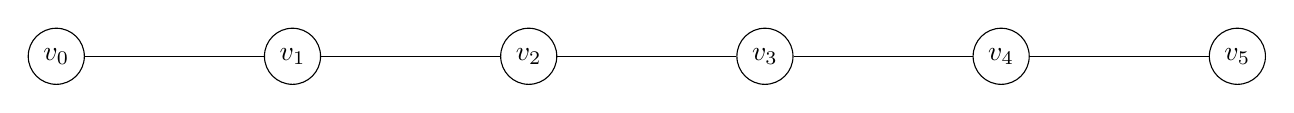
\begin{tikzpicture}[scale=1.5]
  % Define number of vertices (k+1 vertices)
  \def\k{5}  % Path of length k=5
  
  % Place vertices on a horizontal line
  \foreach \i in {0,...,\k} {
    \node[draw, circle, fill=white, minimum size=0.6cm] (v\i) at (\i*2,0) {$v_{\i}$};
  }
  
  % Connect edges
  \foreach \i in {0,...,\number\numexpr\k-1} {
    \pgfmathtruncatemacro{\j}{\i+1}
    \draw (v\i) -- (v\j);
  }
\end{tikzpicture}
\caption{A path graph $P_5$ with 6 vertices.}
\end{figure}

\subsection{Degrees and Neighborhoods}

\begin{definition}
If $G$ is a graph and $v \in V(G)$, then:
\begin{itemize}
\item The neighborhood of $v$ is $N_G(v) = \{w \in V(G) : \{v,w\} \in E(G)\}$
\item The degree of $v$ is $d(v) = d_G(v) = |N_G(v)|$
\end{itemize}
\end{definition}



\begin{figure}[H]
\centering
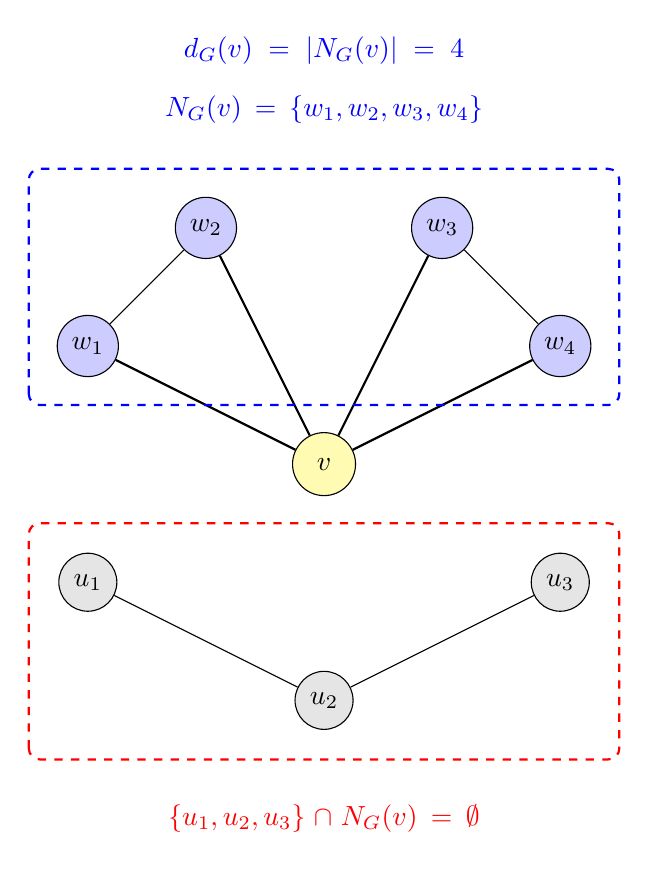
\begin{tikzpicture}[scale=1.5]
  % Central node v
  \node[draw, circle, fill=yellow!30, minimum size=0.8cm] (v) at (0,0) {$v$};
  
  % Neighbors of v
  \node[draw, circle, fill=blue!20, minimum size=0.6cm] (w1) at (-2,1) {$w_1$};
  \node[draw, circle, fill=blue!20, minimum size=0.6cm] (w2) at (-1,2) {$w_2$};
  \node[draw, circle, fill=blue!20, minimum size=0.6cm] (w3) at (1,2) {$w_3$};
  \node[draw, circle, fill=blue!20, minimum size=0.6cm] (w4) at (2,1) {$w_4$};
  
  % Non-neighbor vertices
  \node[draw, circle, fill=gray!20, minimum size=0.6cm] (u1) at (-2,-1) {$u_1$};
  \node[draw, circle, fill=gray!20, minimum size=0.6cm] (u2) at (0,-2) {$u_2$};
  \node[draw, circle, fill=gray!20, minimum size=0.6cm] (u3) at (2,-1) {$u_3$};
  
  % Edges between v and its neighbors
  \draw[thick] (v) -- (w1);
  \draw[thick] (v) -- (w2);
  \draw[thick] (v) -- (w3);
  \draw[thick] (v) -- (w4);
  
  % Other edges
  \draw (w1) -- (w2);
  \draw (w3) -- (w4);
  \draw (u1) -- (u2);
  \draw (u2) -- (u3);
  
  % Neighborhood set indicator
  \draw[blue, thick, dashed, rounded corners] (-2.5,0.5) rectangle (2.5,2.5) {};
  \node[blue, text width=5cm, align=center] at (0,3) {$N_G(v) = \{w_1, w_2, w_3, w_4\}$};
  
  % Degree display - moved and color changed
  \node[blue, text width=5cm, align=center] at (0,3.5) {$d_G(v) = |N_G(v)| = 4$};
  
  % Non-neighbor set indicator
  \draw[red, thick, dashed, rounded corners] (-2.5,-2.5) rectangle (2.5,-0.5) {};
  \node[red, text width=5cm, align=center] at (0,-3) {$\{u_1, u_2, u_3\} \cap N_G(v) = \emptyset$};
\end{tikzpicture}
\caption{Example of neighborhood and degree of a vertex in a graph.}
\end{figure}

\begin{definition}[Incidence]
In graph theory, incidence refers to the relationship between vertices and edges:
\begin{itemize}[label=$\bullet$]
    \item A vertex $v$ and an edge $e$ are \textit{incident} with each other if $v$ is an endpoint of $e$.
    \item If $e = \{u, v\}$, then:
    \begin{itemize}[label=$\circ$]
        \item Edge $e$ is incident with vertices $u$ and $v$
        \item Vertex $u$ is incident with edge $e$
        \item Vertex $v$ is incident with edge $e$
    \end{itemize}
    \item The incidence relation forms the fundamental connection between vertices and edges in a graph.
\end{itemize}
\end{definition}

\subsection{Examples of Graphs and Their Vertex Degrees}

\subsubsection{Complete Graph $K_n$}
In a complete graph with $n$ vertices, every vertex is connected to all other vertices.
\begin{itemize}
    \item For any vertex $v$ in $K_n$: $\deg(v) = n-1$
    \item Example: In $K_5$, every vertex has $\deg(v) = 4$
    \item Total edges: $|E| = \frac{n(n-1)}{2} = \frac{5 \cdot 4}{2} = 10$
\end{itemize}

\begin{figure}[H]
\centering
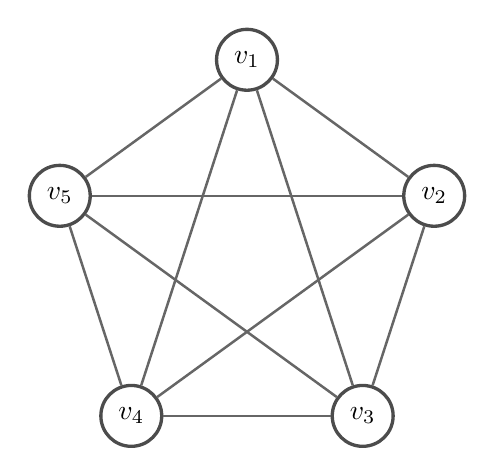
\begin{tikzpicture}
  % Define overall style for the graph
  \tikzset{
    vertex/.style={
      draw,
      circle,
      fill=white,
      minimum size=22pt,
      inner sep=0pt,
      line width=1.2pt,
      draw=black!70
    },
    edge/.style={
      draw=black!60,
      line width=0.9pt
    },
    vlabel/.style={
      font=\sffamily\bfseries,
      text=black!80
    }
  }
  
  % Create vertices at regular pentagon positions
  \def\radius{2.5cm}
  \node[vertex] (v1) at (90:\radius) {$v_1$};
  \node[vertex] (v2) at (18:\radius) {$v_2$};
  \node[vertex] (v3) at (306:\radius) {$v_3$};
  \node[vertex] (v4) at (234:\radius) {$v_4$};
  \node[vertex] (v5) at (162:\radius) {$v_5$};
  
  % Draw all edges
  \foreach \i in {1,...,5} {
    \foreach \j in {\i,...,5} {
      \ifnum\i=\j\else
        \draw[edge] (v\i) -- (v\j);
      \fi
    }
  }
\end{tikzpicture}
\caption{In this complete graph $K_5$ with 5 vertices, each vertex $v_i$ has degree 4. Every vertex is connected to all other vertices in the graph. Total number of edges = $\frac{n(n-1)}{2} = \frac{5 \cdot 4}{2} = 10$}
\end{figure}

\subsubsection{Cycle Graph $C_n$}
A cycle graph with $n$ vertices forms a closed loop.
\begin{itemize}
    \item For any vertex $v$ in $C_n$: $\deg(v) = 2$
    \item Example: In a hexagon $C_6$, every vertex has $\deg(v) = 2$
    \item Total edges: $|E| = n = 6$
\end{itemize}

\begin{center}
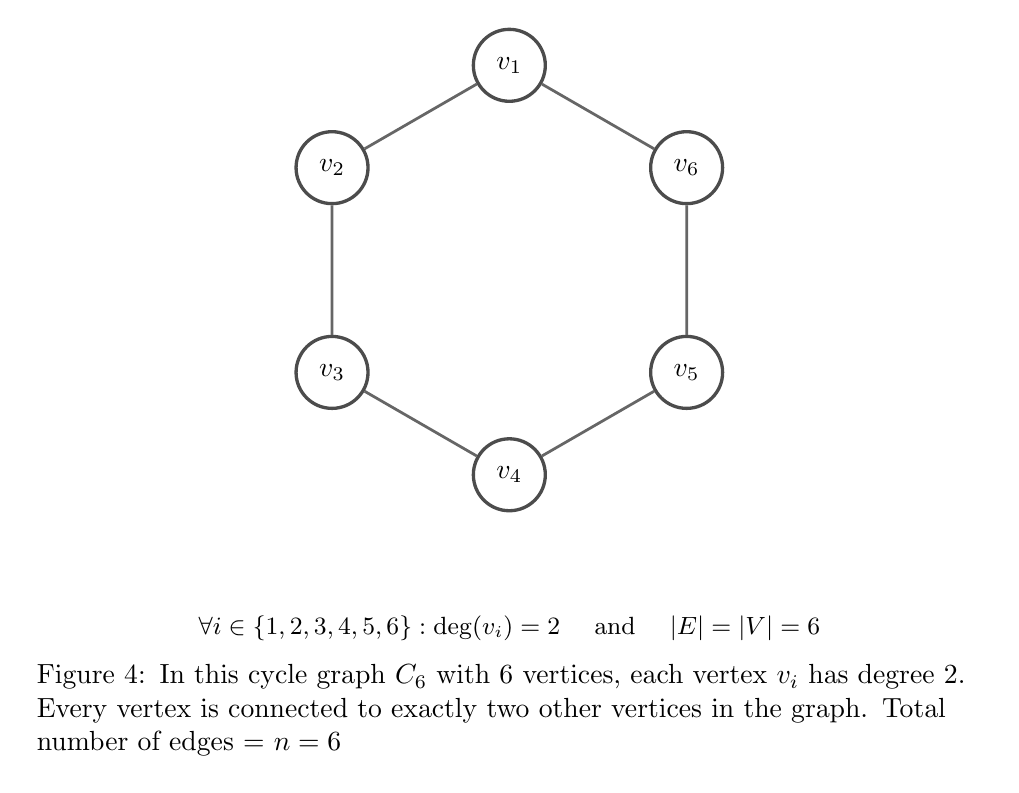
\begin{tikzpicture}[scale=1.3] % Increased scale factor for a larger graph
  % Define styles for vertices
  \tikzset{
    vertex/.style={
      draw,
      circle,
      fill=white,
      minimum size=26pt, % Increased vertex size
      inner sep=0pt,
      line width=1.2pt,
      draw=black!70
    },
    edge/.style={
      draw=black!60,
      line width=1pt % Slightly thicker edges
    }
  }
  
  % Create vertices at regular hexagon positions
  \def\n{6}
  \def\radius{2cm} % Increased radius for larger graph
  
  \foreach \i in {1,...,\n} {
    \node[vertex] (v\i) at ({360/\n*(\i-1)+90}:\radius) {$v_{\i}$};
  }
  
  % Connect vertices to form cycle
  \foreach \i in {1,...,\n} {
    \pgfmathtruncatemacro{\j}{mod(\i, \n) + 1}
    \draw[edge] (v\i) -- (v\j);
  }
  
  % Add compact formula below the graph
  \node[align=center, font=\small] at (0,-3.5) {$\forall i \in \{1,2,3,4,5,6\}: \deg(v_i) = 2 \quad$ and $\quad |E| = |V| = 6$};
  
  % Add Figure 4 caption
  \node[align=left, text width=12cm] at (0,-4.3) {
    Figure 4: In this cycle graph $C_6$ with 6 vertices, each vertex $v_i$ has degree 2. Every vertex is connected to exactly two other vertices in the graph. Total number of edges = $n = 6$
  };
\end{tikzpicture}
\end{center}
\subsubsection{Path Graph $P_n$}
A path graph with $n$ vertices forms a single path.
\begin{itemize}
    \item For endpoints: $\deg(v) = 1$
    \item For internal vertices: $\deg(v) = 2$
    \item Example: In $P_7$, the degree sequence is $(1, 2, 2, 2, 2, 2, 1)$
    \item Total edges: $|E| = n-1 = 6$
\end{itemize}

\begin{center}
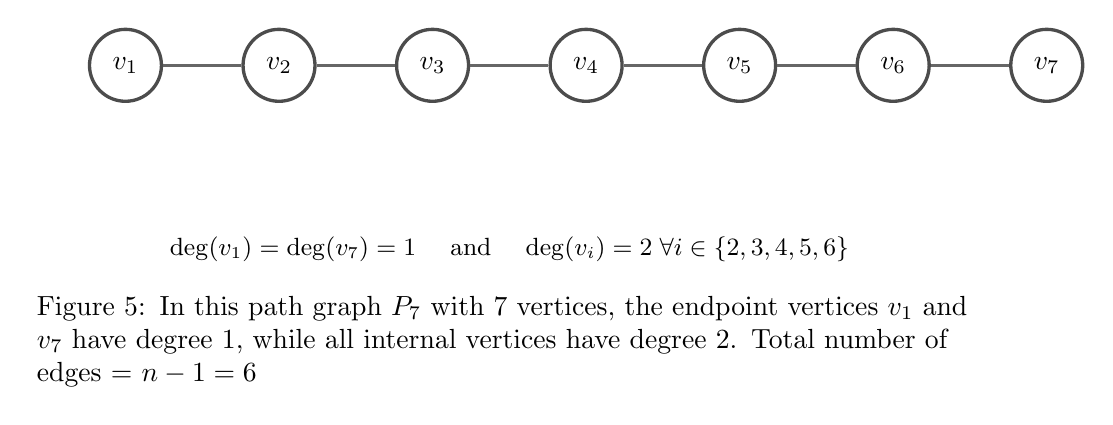
\begin{tikzpicture}[scale=1.3]
  % Define styles for vertices
  \tikzset{
    vertex/.style={
      draw,
      circle,
      fill=white,
      minimum size=26pt,
      inner sep=0pt,
      line width=1.2pt,
      draw=black!70
    },
    edge/.style={
      draw=black!60,
      line width=1pt
    }
  }
  
  % Create vertices in a horizontal line
  \def\n{7}
  \foreach \i in {1,...,\n} {
    \node[vertex] (v\i) at (\i*1.5-1.5*\n/2,0) {$v_{\i}$};
  }
  
  % Connect vertices to form path
  \foreach \i in {1,...,\number\numexpr\n-1} {
    \pgfmathtruncatemacro{\j}{\i+1}
    \draw[edge] (v\i) -- (v\j);
  }
  
  % Add compact formula below the graph
  \node[align=center, font=\small] at (0,-1.8) {$\deg(v_1) = \deg(v_7) = 1 \quad$ and $\quad \deg(v_i) = 2 \; \forall i \in \{2,3,4,5,6\}$};
  
  % Add Figure 5 caption
  \node[align=left, text width=12cm] at (0,-2.7) {
    Figure 5: In this path graph $P_7$ with 7 vertices, the endpoint vertices $v_1$ and $v_7$ have degree 1, while all internal vertices have degree 2. Total number of edges = $n-1 = 6$
  };
\end{tikzpicture}
\end{center}

\subsubsection{Star Graph $S_n$}
A star graph has one central vertex connected to $n-1$ leaf vertices.
\begin{itemize}
    \item For central vertex $c$: $\deg(c) = n-1$
    \item For any leaf vertex $v$: $\deg(v) = 1$
    \item Example: In $S_6$, the central vertex has $\deg(c) = 5$, and the 5 leaf vertices each have $\deg(v) = 1$
    \item Total edges: $|E| = n-1 = 5$
\end{itemize}

\begin{center}
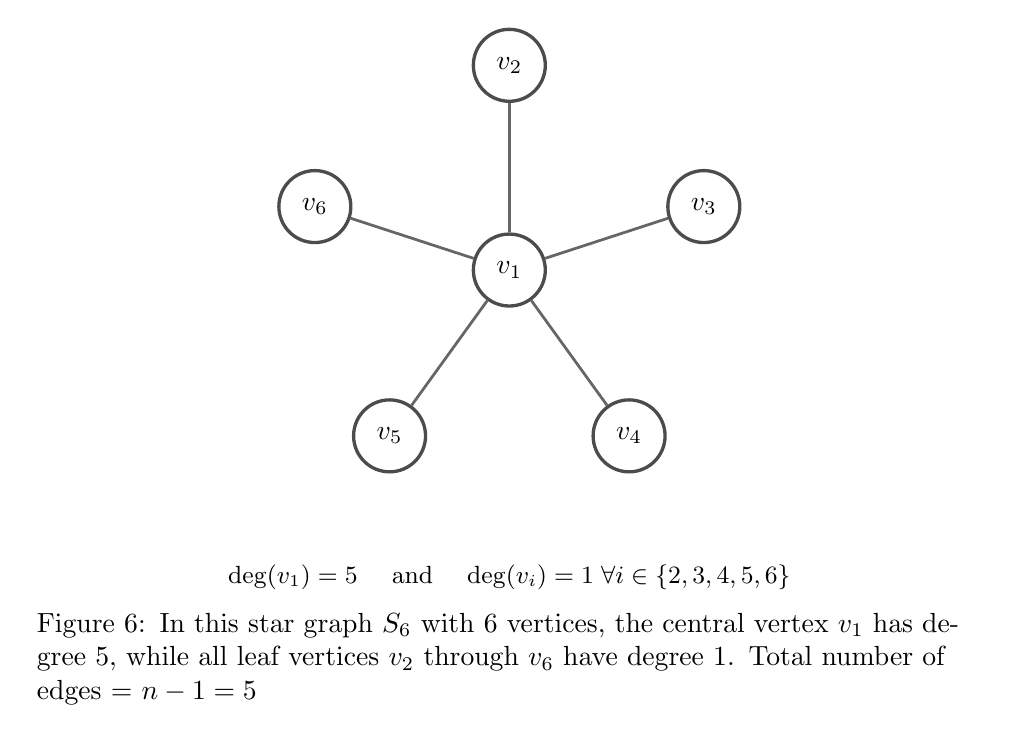
\begin{tikzpicture}[scale=1.3]
  % Define styles for vertices
  \tikzset{
    vertex/.style={
      draw,
      circle,
      fill=white,
      minimum size=26pt,
      inner sep=0pt,
      line width=1.2pt,
      draw=black!70
    },
    edge/.style={
      draw=black!60,
      line width=1pt
    }
  }
  
  % Create vertices - central and leaf vertices
  \node[vertex] (v1) at (0,0) {$v_1$};
  \node[vertex] (v2) at (0,2) {$v_2$};
  \node[vertex] (v3) at (1.9,0.62) {$v_3$};
  \node[vertex] (v4) at (1.17,-1.62) {$v_4$};
  \node[vertex] (v5) at (-1.17,-1.62) {$v_5$};
  \node[vertex] (v6) at (-1.9,0.62) {$v_6$};
  
  % Connect edges
  \draw[edge] (v1) -- (v2);
  \draw[edge] (v1) -- (v3);
  \draw[edge] (v1) -- (v4);
  \draw[edge] (v1) -- (v5);
  \draw[edge] (v1) -- (v6);
  
  % Add compact formula below the graph
  \node[align=center, font=\small] at (0,-3) {$\deg(v_1) = 5 \quad$ and $\quad \deg(v_i) = 1 \; \forall i \in \{2,3,4,5,6\}$};
  
  % Add Figure 6 caption
  \node[align=left, text width=12cm] at (0,-3.8) {
    Figure 6: In this star graph $S_6$ with 6 vertices, the central vertex $v_1$ has degree 5, while all leaf vertices $v_2$ through $v_6$ have degree 1. Total number of edges = $n-1 = 5$
  };
\end{tikzpicture}
\end{center}

\subsubsection{Wheel Graph $W_n$}
A wheel graph is formed by connecting a single vertex to all vertices of a cycle.
\begin{itemize}
    \item For central vertex $c$: $\deg(c) = n-1$
    \item For vertices on the cycle: $\deg(v) = 3$
    \item Example: In $W_8$, the central vertex has $\deg(c) = 7$, and the 7 outer vertices each have $\deg(v) = 3$
    \item Total edges: $|E| = 2(n-1) = 14$
\end{itemize}

\begin{center}
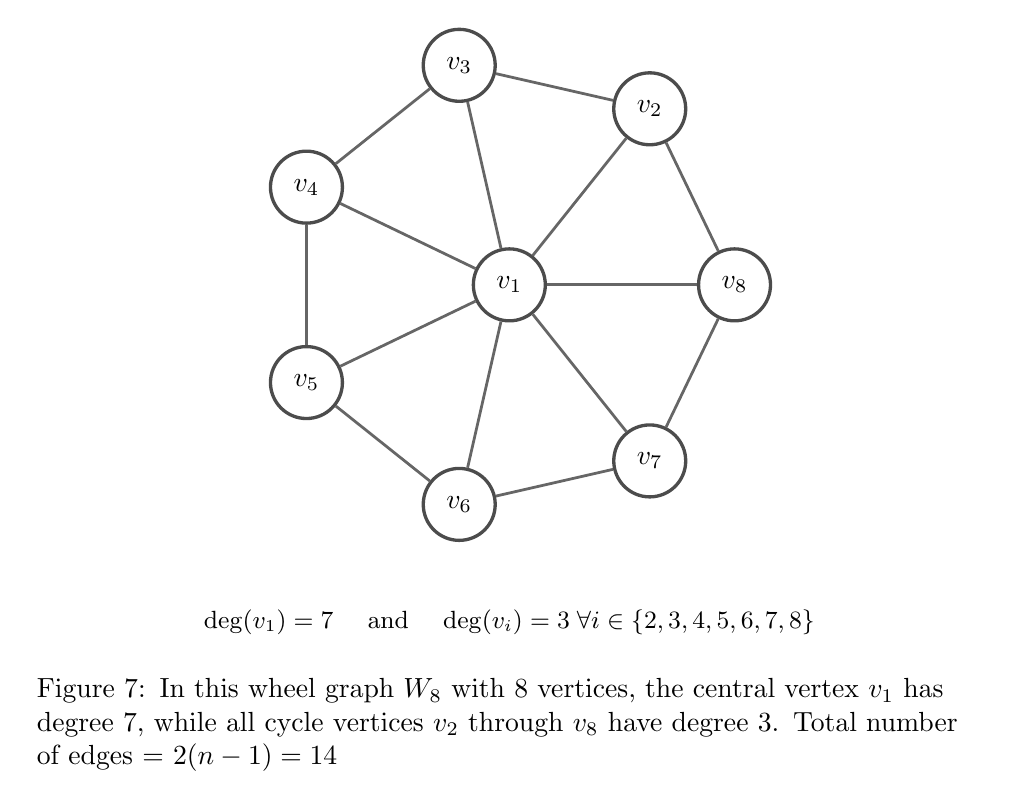
\begin{tikzpicture}[scale=1.3]
  % Define styles for vertices
  \tikzset{
    vertex/.style={
      draw,
      circle,
      fill=white,
      minimum size=26pt,
      inner sep=0pt,
      line width=1.2pt,
      draw=black!70
    },
    edge/.style={
      draw=black!60,
      line width=1pt
    }
  }
  
  % Create central vertex
  \node[vertex] (v1) at (0,0) {$v_1$};
  
  % Create outer cycle vertices
  \def\n{7}
  \def\radius{2.2cm}
  
  \foreach \i in {2,...,\number\numexpr\n+1} {
    \pgfmathtruncatemacro{\j}{\i-1}
    \node[vertex] (v\i) at ({360/\n*\j}:\radius) {$v_{\i}$};
  }
  
  % Draw cycle edges
  \foreach \i in {2,...,\number\numexpr\n+1} {
    \pgfmathtruncatemacro{\j}{mod(\i-1, \n) + 2}
    \draw[edge] (v\i) -- (v\j);
  }
  
  % Draw spokes from center to cycle
  \foreach \i in {2,...,\number\numexpr\n+1} {
    \draw[edge] (v1) -- (v\i);
  }
  
  % Add compact formula below the graph
  \node[align=center, font=\small] at (0,-3.3) {$\deg(v_1) = 7 \quad$ and $\quad \deg(v_i) = 3 \; \forall i \in \{2,3,4,5,6,7,8\}$};
  
  % Add Figure 7 caption
  \node[align=left, text width=12cm] at (0,-4.3) {
    Figure 7: In this wheel graph $W_8$ with 8 vertices, the central vertex $v_1$ has degree 7, while all cycle vertices $v_2$ through $v_8$ have degree 3. Total number of edges = $2(n-1) = 14$
  };
\end{tikzpicture}
\end{center}

\subsubsection{Complete Bipartite Graph $K_{m,n}$}
A complete bipartite graph has two sets of vertices (with $m$ and $n$ vertices) where every vertex in the first set is connected to every vertex in the second set.
\begin{itemize}
    \item For vertices in the first set: $\deg(v) = n$
    \item For vertices in the second set: $\deg(v) = m$
    \item Example: In $K_{3,4}$, the 3 vertices in the first set each have $\deg(v) = 4$, and the 4 vertices in the second set each have $\deg(v) = 3$
    \item Total edges: $|E| = m \cdot n = 12$
\end{itemize}

\begin{center}
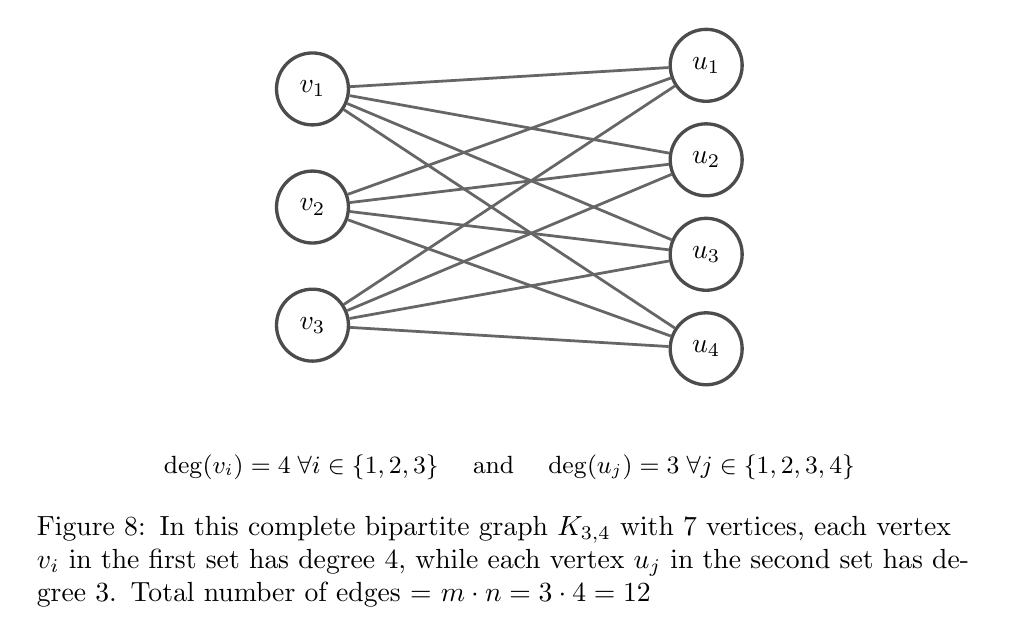
\begin{tikzpicture}[scale=1.0]
  % Define styles for vertices
  \tikzset{
    vertex/.style={
      draw,
      circle,
      fill=white,
      minimum size=26pt,
      inner sep=0pt,
      line width=1.2pt,
      draw=black!70
    },
    edge/.style={
      draw=black!60,
      line width=1pt
    }
  }
  
  % Left set (m=3)
  \node[vertex] (v1) at (-2.5,1.5) {$v_1$};
  \node[vertex] (v2) at (-2.5,0) {$v_2$};
  \node[vertex] (v3) at (-2.5,-1.5) {$v_3$};
  
  % Right set (n=4)
  \node[vertex] (u1) at (2.5,1.8) {$u_1$};
  \node[vertex] (u2) at (2.5,0.6) {$u_2$};
  \node[vertex] (u3) at (2.5,-0.6) {$u_3$};
  \node[vertex] (u4) at (2.5,-1.8) {$u_4$};
  
  % Connect each vertex in left set to each vertex in right set
  \foreach \i in {1,2,3} {
    \foreach \j in {1,2,3,4} {
      \draw[edge] (v\i) -- (u\j);
    }
  }
  
  % Add compact formula below the graph
  \node[align=center, font=\small] at (0,-3.3) {$\deg(v_i) = 4 \; \forall i \in \{1,2,3\} \quad$ and $\quad \deg(u_j) = 3 \; \forall j \in \{1,2,3,4\}$};
  
  % Add Figure 8 caption
  \node[align=left, text width=12cm] at (0,-4.5) {
    Figure 8: In this complete bipartite graph $K_{3,4}$ with 7 vertices, each vertex $v_i$ in the first set has degree 4, while each vertex $u_j$ in the second set has degree 3. Total number of edges = $m \cdot n = 3 \cdot 4 = 12$
  };
\end{tikzpicture}
\end{center}

\subsubsection{Regular Graph}
In a $k$-regular graph, every vertex has the same degree $k$.
\begin{itemize}
    \item For any vertex $v$: $\deg(v) = k$
    \item Example: In a 3-regular graph (cubic graph), every vertex has $\deg(v) = 3$
    \item Total edges in a $k$-regular graph with $n$ vertices: $|E| = \frac{kn}{2}$
\end{itemize}

\begin{center}
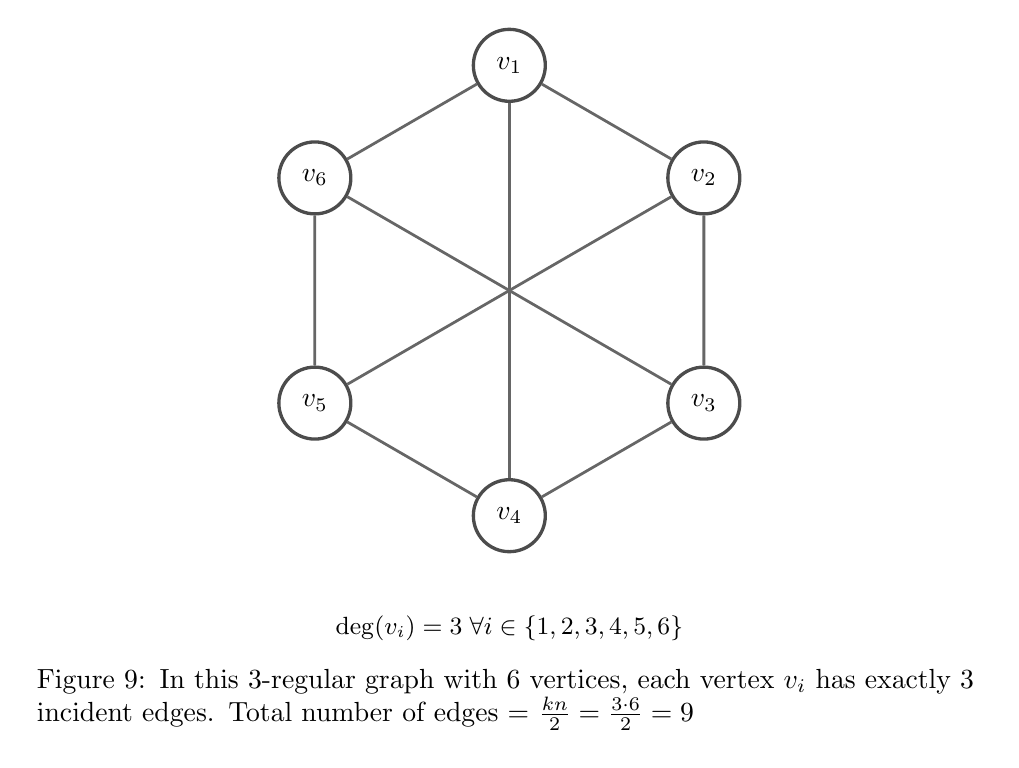
\begin{tikzpicture}[scale=1.3]
  \tikzset{
    vertex/.style={
      draw,
      circle,
      fill=white,
      minimum size=26pt,
      inner sep=0pt,
      line width=1.2pt,
      draw=black!70
    },
    edge/.style={
      draw=black!60,
      line width=1pt
    }
  }
  
  \node[vertex] (v1) at (0,2.2) {$v_1$};
  \node[vertex] (v2) at (1.9,1.1) {$v_2$};
  \node[vertex] (v3) at (1.9,-1.1) {$v_3$};
  \node[vertex] (v4) at (0,-2.2) {$v_4$};
  \node[vertex] (v5) at (-1.9,-1.1) {$v_5$};
  \node[vertex] (v6) at (-1.9,1.1) {$v_6$};
  
  \draw[edge] (v1) -- (v2) -- (v3) -- (v4) -- (v5) -- (v6) -- (v1);
  \draw[edge] (v1) -- (v4);
  \draw[edge] (v2) -- (v5);
  \draw[edge] (v3) -- (v6);
  
  \node[align=center, font=\small] at (0,-3.3) {$\deg(v_i) = 3 \; \forall i \in \{1,2,3,4,5,6\}$};
  
  \node[align=left, text width=12cm] at (0,-4.0) {
    Figure 9: In this 3-regular graph with 6 vertices, each vertex $v_i$ has exactly 3 incident edges. Total number of edges = $\frac{kn}{2} = \frac{3 \cdot 6}{2} = 9$
  };
\end{tikzpicture}
\end{center}


\subsubsection{Hypercube Graph $Q_n$}
In an $n$-dimensional hypercube, every vertex has degree $n$.
\begin{itemize}
    \item For any vertex $v$ in $Q_n$: $\deg(v) = n$
    \item Example: In $Q_3$ (3-dimensional cube), every vertex has $\deg(v) = 3$
    \item Total vertices: $|V| = 2^n$
    \item Total edges: $|E| = n \cdot 2^{n-1}$
\end{itemize}

\begin{center}
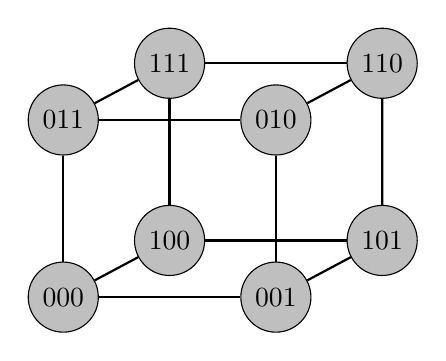
\begin{tikzpicture}[scale=0.9]
  % Q_3 (3-dimensional hypercube)
  % Front square
  \node[draw, circle, fill=lightgray, minimum size=0.7cm] (v000) at (0,0) {$000$};
  \node[draw, circle, fill=lightgray, minimum size=0.7cm] (v001) at (3,0) {$001$};
  \node[draw, circle, fill=lightgray, minimum size=0.7cm] (v010) at (3,2.5) {$010$};
  \node[draw, circle, fill=lightgray, minimum size=0.7cm] (v011) at (0,2.5) {$011$};
  
  % Back square
  \node[draw, circle, fill=lightgray, minimum size=0.7cm] (v100) at (1.5,0.8) {$100$};
  \node[draw, circle, fill=lightgray, minimum size=0.7cm] (v101) at (4.5,0.8) {$101$};
  \node[draw, circle, fill=lightgray, minimum size=0.7cm] (v110) at (4.5,3.3) {$110$};
  \node[draw, circle, fill=lightgray, minimum size=0.7cm] (v111) at (1.5,3.3) {$111$};
  
  % Front face edges
  \draw[thick] (v000) -- (v001);
  \draw[thick] (v001) -- (v010);
  \draw[thick] (v010) -- (v011);
  \draw[thick] (v011) -- (v000);
  
  % Back face edges
  \draw[thick] (v100) -- (v101);
  \draw[thick] (v101) -- (v110);
  \draw[thick] (v110) -- (v111);
  \draw[thick] (v111) -- (v100);
  
  % Connections between front and back faces
  \draw[thick] (v000) -- (v100);
  \draw[thick] (v001) -- (v101);
  \draw[thick] (v010) -- (v110);
  \draw[thick] (v011) -- (v111);
\end{tikzpicture}
\end{center}

\begin{center}
    \vspace{0.5cm}
{\centering
\small $\deg(v) = 3 \; \forall v \in V(Q_3)$
\par}

\vspace{0.5cm}
{\centering
\footnotesize Figure 10: Hypercube graph $Q_3$ with vertices labeled by binary strings. Each vertex has degree 3, with connections to neighbors that differ in exactly one bit position.
\par}
\end{center}

\subsubsection{Petersen Graph}
The Petersen graph is a specific 3-regular graph with 10 vertices.
\begin{itemize}
    \item For any vertex $v$: $\deg(v) = 3$
    \item Total edges: $|E| = 15$
\end{itemize}

\begin{center}
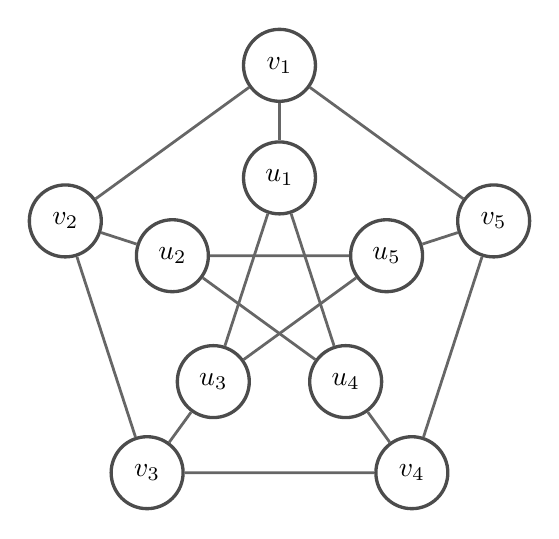
\begin{tikzpicture}[scale=1.3]
  \tikzset{
    vertex/.style={
      draw,
      circle,
      fill=white,
      minimum size=26pt,
      inner sep=0pt,
      line width=1.2pt,
      draw=black!70
    },
    edge/.style={
      draw=black!60,
      line width=1pt
    }
  }
  
  % Outer vertices
  \foreach \i in {1,...,5} {
    \node[vertex] (v\i) at ({90+72*(\i-1)}:2.2) {$v_{\i}$};
  }
  
  % Inner vertices
  \foreach \i in {1,...,5} {
    \node[vertex] (u\i) at ({90+72*(\i-1)}:1.1) {$u_{\i}$};
  }
  
  % Outer edges
  \foreach \i in {1,...,5} {
    \pgfmathtruncatemacro{\j}{mod(\i,5)+1}
    \draw[edge] (v\i) -- (v\j);
  }
  
  % Spoke edges
  \foreach \i in {1,...,5} {
    \draw[edge] (v\i) -- (u\i);
  }
  
  % Inner star edges
  \foreach \i in {1,...,5} {
    \pgfmathtruncatemacro{\j}{mod(\i+1,5)+1}
    \draw[edge] (u\i) -- (u\j);
  }
\end{tikzpicture}
\end{center}

% Formula and caption
\vspace{0.5cm}
{\centering
\small $\deg(v_i) = \deg(u_i) = 3 \; \forall i \in \{1,2,3,4,5\}$
\par}

\vspace{0.5cm}
{\centering
\footnotesize Figure 11: Petersen graph with 10 vertices. Each vertex has degree 3, with a total of 15 edges. This is a famous non-Hamiltonian 3-regular graph.
\par}

\subsection{Mathematical Properties Related to Degrees}

\subsubsection{Handshaking Lemma}
The sum of all degrees equals twice the number of edges:
\begin{equation}
\sum_{v \in V} \deg(v) = 2|E|
\end{equation}

\begin{center}
\begin{tikzpicture}[scale=1.5]
  \tikzset{
    vertex/.style={
      draw,
      circle,
      fill=white,
      minimum size=26pt,
      inner sep=0pt,
      line width=1.2pt,
      draw=black!70
    },
    edge/.style={
      draw=black!60,
      line width=1pt
    },
    elabel/.style={
      midway,
      font=\small
    }
  }
\end{tikzpicture}
\end{center}
  
\begin{center}
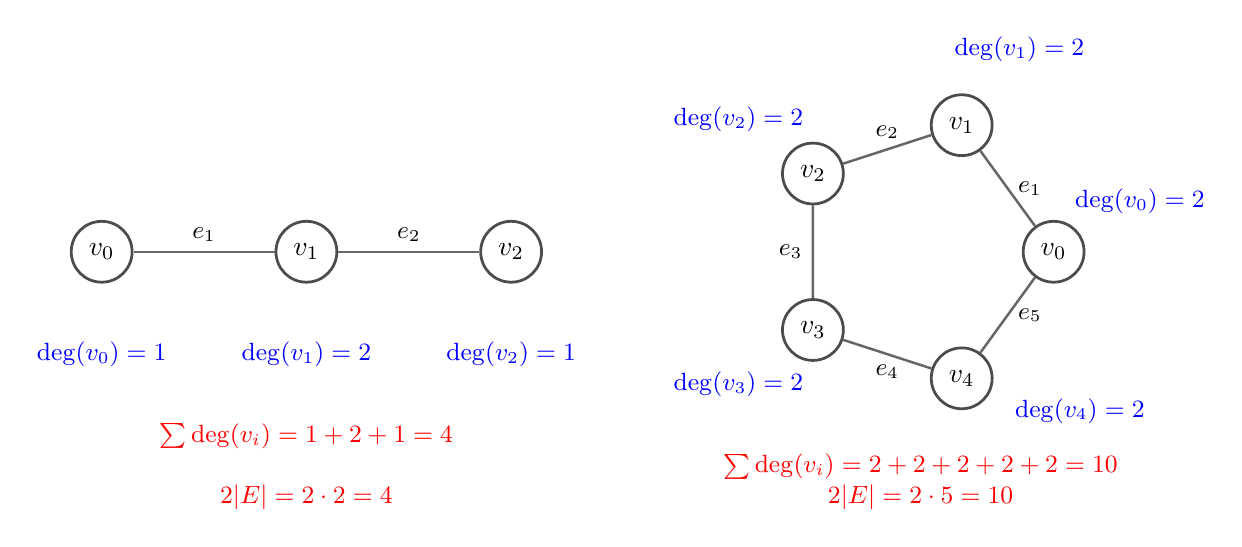
\begin{tikzpicture}[scale=1.3]
  \tikzset{
    vertex/.style={
      draw,
      circle,
      fill=white,
      minimum size=22pt,
      inner sep=0pt,
      line width=1pt,
      draw=black!70
    },
    edge/.style={
      draw=black!60,
      line width=0.9pt
    },
    elabel/.style={
      midway,
      font=\small
    }
  }
  
  % First example: Path graph
  \begin{scope}[shift={(-4,0)}]
    % Vertices
    \node[vertex] (v0) at (0,0) {$v_0$};
    \node[vertex] (v1) at (2,0) {$v_1$};
    \node[vertex] (v2) at (4,0) {$v_2$};
    
    % Edges
    \draw[edge] (v0) -- (v1) node[elabel, above] {$e_1$};
    \draw[edge] (v1) -- (v2) node[elabel, above] {$e_2$};
    
    % Degree display
    \node[font=\small, text=blue] at (0,-1) {$\deg(v_0) = 1$};
    \node[font=\small, text=blue] at (2,-1) {$\deg(v_1) = 2$};
    \node[font=\small, text=blue] at (4,-1) {$\deg(v_2) = 1$};
    
    % Sum calculation
    \node[font=\small, text=red] at (2,-1.8) {$\sum \deg(v_i) = 1 + 2 + 1 = 4$};
    \node[font=\small, text=red] at (2,-2.4) {$2|E| = 2 \cdot 2 = 4$};
  \end{scope}
  
  % Second example: Cycle graph
  \begin{scope}[shift={(4,0)}]
    % Vertices
    \node[vertex] (v0) at (0:1.3cm) {$v_0$};
    \node[vertex] (v1) at (72:1.3cm) {$v_1$};
    \node[vertex] (v2) at (144:1.3cm) {$v_2$};
    \node[vertex] (v3) at (216:1.3cm) {$v_3$};
    \node[vertex] (v4) at (288:1.3cm) {$v_4$};
    
    % Edges
    \draw[edge] (v0) -- (v1) node[elabel, right] {$e_1$};
    \draw[edge] (v1) -- (v2) node[elabel, above] {$e_2$};
    \draw[edge] (v2) -- (v3) node[elabel, left] {$e_3$};
    \draw[edge] (v3) -- (v4) node[elabel, below] {$e_4$};
    \draw[edge] (v4) -- (v0) node[elabel, right] {$e_5$};
    
    % Degree display
    \node[font=\small, text=blue] at (13:2.2cm) {$\deg(v_0) = 2$};
    \node[font=\small, text=blue] at (64:2.2cm) {$\deg(v_1) = 2$};
    \node[font=\small, text=blue] at (144:2.2cm) {$\deg(v_2) = 2$};
    \node[font=\small, text=blue] at (216:2.2cm) {$\deg(v_3) = 2$};
    \node[font=\small, text=blue] at (315:2.2cm) {$\deg(v_4) = 2$};
    
    % Sum calculation
    \node[font=\small, text=red] at (0,-2.1) {$\sum \deg(v_i) = 2 + 2 + 2 + 2 + 2 = 10$};
    \node[font=\small, text=red] at (0,-2.4) {$2|E| = 2 \cdot 5 = 10$};
  \end{scope}
\end{tikzpicture}
\end{center}

% Caption
\vspace{0.3cm}
{\centering
\footnotesize Figure 12 and 13: Illustration of the Handshaking Lemma. Left: A path graph with 3 vertices and 2 edges. Right: A cycle graph with 5 vertices and 5 edges. In both cases, the sum of vertex degrees equals twice the number of edges.
\par}
\begin{example}
Consider a graph with vertex set $V = \{1, 2, 3, 4\}$ and edge set $E = \{\{1,2\}, \{1,3\}, \{1,4\}, \{2,3\}, \{3,4\}\}$.
\begin{align*}
\sum_{v \in V} d(v) &= d(1) + d(2) + d(3) + d(4)\\
&= 3 + 2 + 3 + 2\\
&= 10
\end{align*}
And $2|E| = 2 \cdot 5 = 10$.
\end{example}

\subsubsection{Degree Sequence}
The non-increasing sequence of vertex degrees.
\begin{itemize}
    \item Example: A graph with degree sequence $(4,3,3,2,2,1,1)$ has 7 vertices with varying connectivity
    \item Valid degree sequences must sum to an even number
\end{itemize}
\subsubsection{Average Degree}
The average degree of vertices in a graph $G = (V,E)$ is:
\begin{equation}
\text{avg}(\deg) = \frac{\sum_{v \in V} \deg(v)}{|V|} = \frac{2|E|}{|V|}
\end{equation}
\subsubsection{Maximum and Minimum Degree}
\begin{align}
\Delta(G) &= \max\{\deg(v) \mid v \in V\} \\
\delta(G) &= \min\{\deg(v) \mid v \in V\}
\end{align}
\begin{corollary}
In any graph, there are an even number of vertices of odd degree.
\end{corollary}

\begin{center}
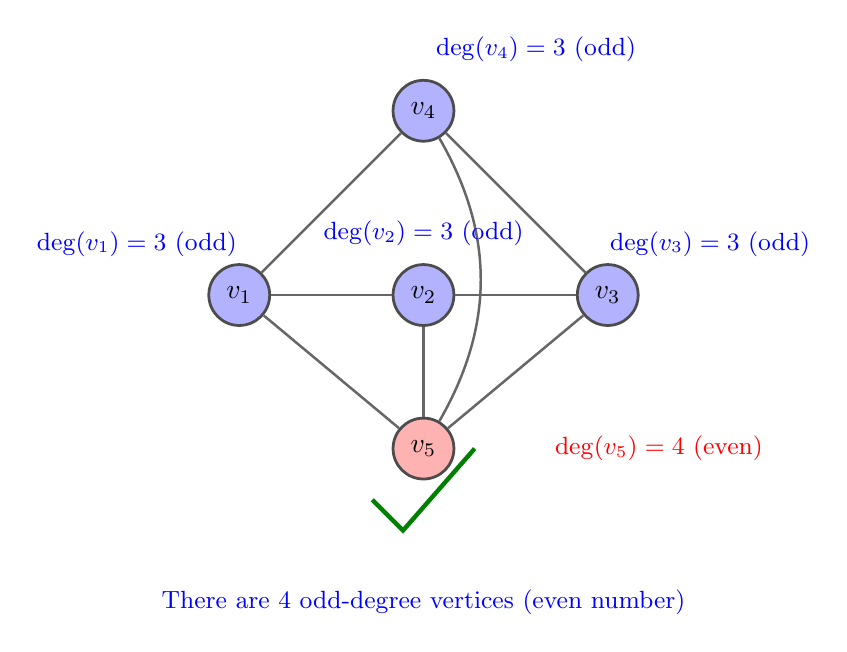
\begin{tikzpicture}[scale=1.3]
  \tikzset{
    vertex/.style={
      draw,
      circle,
      fill=white,
      minimum size=22pt,
      inner sep=0pt,
      line width=1pt,
      draw=black!70
    },
    oddvertex/.style={
      draw,
      circle,
      fill=blue!30,
      minimum size=22pt,
      inner sep=0pt,
      line width=1pt,
      draw=black!70
    },
    evenvertex/.style={
      draw,
      circle,
      fill=red!30,
      minimum size=22pt,
      inner sep=0pt,
      line width=1pt,
      draw=black!70
    },
    edge/.style={
      draw=black!60,
      line width=0.9pt
    }
  }
  
  % Nodes
  \node[oddvertex] (v1) at (-1.8,0) {$v_1$};
  \node[oddvertex] (v2) at (0,0) {$v_2$};
  \node[oddvertex] (v3) at (1.8,0) {$v_3$};
  \node[oddvertex] (v4) at (0,1.8) {$v_4$};
  \node[evenvertex] (v5) at (0,-1.5) {$v_5$};
  
  % Edges
  \draw[edge] (v1) -- (v2);
  \draw[edge] (v2) -- (v3);
  \draw[edge] (v1) -- (v4);
  \draw[edge] (v3) -- (v4);
  \draw[edge] (v1) -- (v5);
  \draw[edge] (v2) -- (v5);
  \draw[edge] (v3) -- (v5);
  \draw[edge] (v4) to[bend left=30] (v5);
  
  % Degree display
  \node[align=center, blue, font=\small] at (-2.8,0.5) {$\deg(v_1)=3$ (odd)};
  \node[align=center, blue, font=\small] at (0,0.6) {$\deg(v_2)=3$ (odd)};
  \node[align=center, blue, font=\small] at (2.8,0.5) {$\deg(v_3)=3$ (odd)};
  \node[align=center, blue, font=\small] at (1.1,2.4) {$\deg(v_4)=3$ (odd)};
  \node[align=center, red, font=\small] at (2.3,-1.5) {$\deg(v_5)=4$ (even)};
  
  % Green checkmark
  \draw[ultra thick, green!50!black] (-0.5,-2) -- (-0.2,-2.3) -- (0.5,-1.5);
  
  % Conclusion
  \node[align=center, blue, font=\small] at (0,-3) {There are 4 odd-degree vertices (even number)};
\end{tikzpicture}
\end{center}

% Caption
\vspace{0.3cm}
{\centering
\footnotesize Figure 14: A graph illustrating the handshaking lemma's corollary that any graph must contain an even number of odd-degree vertices. This example has 4 vertices with odd degree (shown in blue) and 1 vertex with even degree (shown in red).
\par}

\subsubsection{Isolated and Pendant Vertices}
\begin{itemize}
    \item Isolated vertex: $\deg(v) = 0$
    \item Pendant vertex (leaf): $\deg(v) = 1$
    \item Example: A tree with $n$ vertices has exactly $n-2$ vertices of degree $\geq 2$ and at least 2 leaves
\end{itemize}
\begin{center}
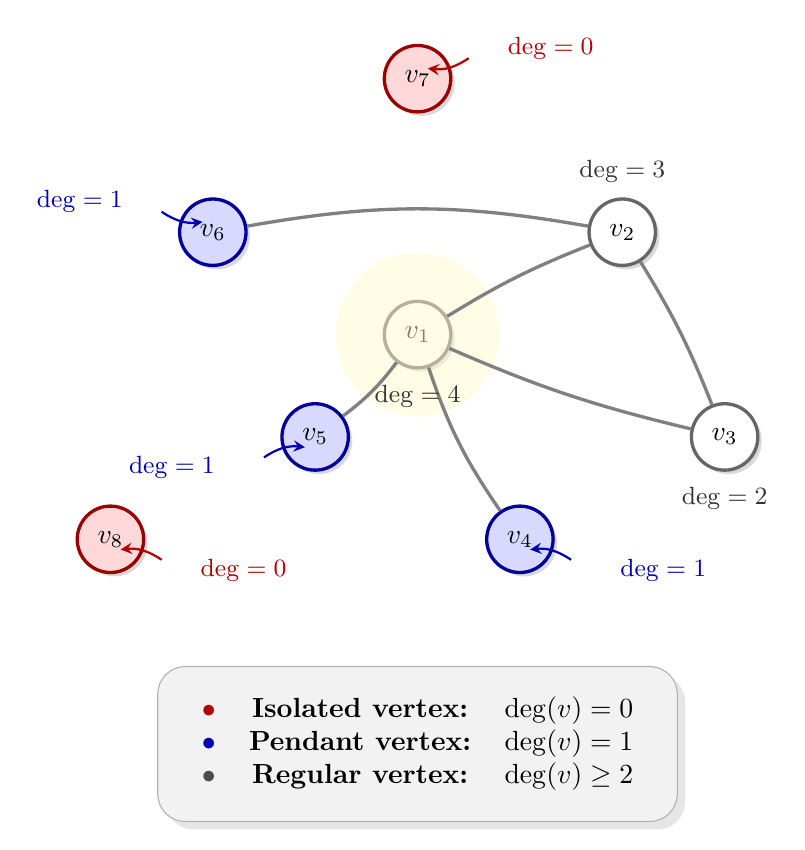
\begin{tikzpicture}[scale=1.3]
  \tikzset{
    vertex/.style={
      draw,
      circle,
      fill=white,
      minimum size=24pt,
      inner sep=0pt,
      line width=1.2pt,
      draw=black!60,
      drop shadow={shadow xshift=0.5mm, shadow yshift=-0.5mm, opacity=0.3}
    },
    isolatedvertex/.style={
      draw,
      circle,
      fill=red!15,
      minimum size=24pt,
      inner sep=0pt,
      line width=1.2pt,
      draw=red!60!black,
      drop shadow={shadow xshift=0.5mm, shadow yshift=-0.5mm, opacity=0.3}
    },
    pendantvertex/.style={
      draw,
      circle,
      fill=blue!15,
      minimum size=24pt,
      inner sep=0pt,
      line width=1.2pt,
      draw=blue!60!black,
      drop shadow={shadow xshift=0.5mm, shadow yshift=-0.5mm, opacity=0.3}
    },
    edge/.style={
      draw=black!50,
      line width=1.2pt
    },
    label/.style={
      font=\sffamily\small,
      align=center
    }
  }
  
  % Create a graph with isolated and pendant vertices
  \node[vertex] (v1) at (0,0) {$v_1$};
  \node[vertex] (v2) at (2,1) {$v_2$};
  \node[vertex] (v3) at (3,-1) {$v_3$};
  \node[pendantvertex] (v4) at (1,-2) {$v_4$};
  \node[pendantvertex] (v5) at (-1,-1) {$v_5$};
  \node[pendantvertex] (v6) at (-2,1) {$v_6$};
  \node[isolatedvertex] (v7) at (0,2.5) {$v_7$};
  \node[isolatedvertex] (v8) at (-3,-2) {$v_8$};
  
  % Add node highlights
  \path[fill=yellow!20, opacity=0.5] (v1.center) circle (0.8cm);
  
  % Connect edges with slight curves for aesthetics
  \draw[edge] (v1) to[bend left=5] (v2);
  \draw[edge] (v1) to[bend right=5] (v3);
  \draw[edge] (v2) to[bend left=5] (v3);
  \draw[edge] (v1) to[bend right=8] (v4);
  \draw[edge] (v1) to[bend left=8] (v5);
  \draw[edge] (v2) to[bend right=10] (v6);
  
  % Add degree information with elegant styling
  \node[label, text=black!80] at (0,-0.6) {$\deg=4$};
  \node[label, text=black!80] at (2,1.6) {$\deg=3$};
  \node[label, text=black!80] at (3,-1.6) {$\deg=2$};
  
  % Pendant vertices labels with elegant arrows
  \draw[->, thick, blue!70!black, >=stealth] (1.5,-2.2) to[bend right=20] (1.1,-2.1);
  \node[label, text=blue!70!black] at (2.4,-2.3) {$\deg=1$};
  
  \draw[->, thick, blue!70!black, >=stealth] (-1.5,-1.2) to[bend left=20] (-1.1,-1.1);
  \node[label, text=blue!70!black] at (-2.4,-1.3) {$\deg=1$};
  
  \draw[->, thick, blue!70!black, >=stealth] (-2.5,1.2) to[bend right=20] (-2.1,1.1);
  \node[label, text=blue!70!black] at (-3.3,1.3) {$\deg=1$};
  
  % Isolated vertices labels with elegant arrows
  \draw[->, thick, red!70!black, >=stealth] (0.5,2.7) to[bend left=20] (0.1,2.6);
  \node[label, text=red!70!black] at (1.3,2.8) {$\deg=0$};
  
  \draw[->, thick, red!70!black, >=stealth] (-2.5,-2.2) to[bend right=20] (-2.9,-2.1);
  \node[label, text=red!70!black] at (-1.7,-2.3) {$\deg=0$};
  
  % Add stylish legend
  \node[draw=black!30, rounded corners=10pt, fill=black!5, inner sep=10pt, drop shadow={shadow xshift=1mm, shadow yshift=-1mm, opacity=0.2}] at (0,-4) {
    \begin{tabular}{lcl}
      \textcolor{red!70!black}{$\bullet$} & \textbf{Isolated vertex:} & $\deg(v) = 0$ \\
      \textcolor{blue!70!black}{$\bullet$} & \textbf{Pendant vertex:} & $\deg(v) = 1$ \\
      \textcolor{black!70}{$\bullet$} & \textbf{Regular vertex:} & $\deg(v) \geq 2$ \\
    \end{tabular}
  };
\end{tikzpicture}
\end{center}

% Caption
\vspace{0.3cm}
{\centering
\footnotesize Figure 15: Illustration of special vertex types based on degree. The center vertex $v_1$ (highlighted) connects to both regular vertices and pendant vertices, while isolated vertices remain disconnected from the graph.
\par}

\subsection{Subgraphs}
\begin{definition}
A graph $F$ is a subgraph of graph $G$ if $V(F) \subseteq V(G)$ and $E(F) \subseteq E(G)$, written $F \subseteq G$.
\end{definition}

\begin{center}
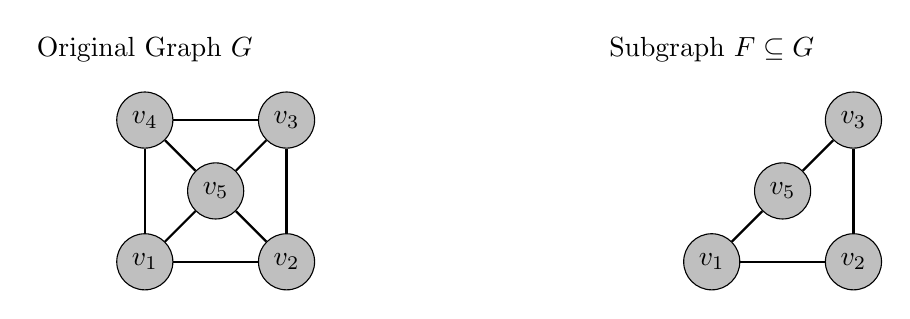
\begin{tikzpicture}[scale=0.9]
  % Original graph G
  \begin{scope}[shift={(-4,0)}]
    \node[align=center] at (0,3) {Original Graph $G$};
    
    % Vertices
    \node[draw, circle, fill=lightgray, minimum size=0.7cm] (v1) at (0,0) {$v_1$};
    \node[draw, circle, fill=lightgray, minimum size=0.7cm] (v2) at (2,0) {$v_2$};
    \node[draw, circle, fill=lightgray, minimum size=0.7cm] (v3) at (2,2) {$v_3$};
    \node[draw, circle, fill=lightgray, minimum size=0.7cm] (v4) at (0,2) {$v_4$};
    \node[draw, circle, fill=lightgray, minimum size=0.7cm] (v5) at (1,1) {$v_5$};
    
    % Edges
    \draw[thick] (v1) -- (v2);
    \draw[thick] (v2) -- (v3);
    \draw[thick] (v3) -- (v4);
    \draw[thick] (v4) -- (v1);
    \draw[thick] (v1) -- (v5);
    \draw[thick] (v2) -- (v5);
    \draw[thick] (v3) -- (v5);
    \draw[thick] (v4) -- (v5);
  \end{scope}
  
  % Subgraph F
  \begin{scope}[shift={(4,0)}]
    \node[align=center] at (0,3) {Subgraph $F \subseteq G$};
    
    % Vertices
    \node[draw, circle, fill=lightgray, minimum size=0.7cm] (u1) at (0,0) {$v_1$};
    \node[draw, circle, fill=lightgray, minimum size=0.7cm] (u2) at (2,0) {$v_2$};
    \node[draw, circle, fill=lightgray, minimum size=0.7cm] (u3) at (2,2) {$v_3$};
    \node[draw, circle, fill=lightgray, minimum size=0.7cm] (u5) at (1,1) {$v_5$};
    
    % Selected edges
    \draw[thick] (u1) -- (u2);
    \draw[thick] (u2) -- (u3);
    \draw[thick] (u1) -- (u5);
    \draw[thick] (u3) -- (u5);
  \end{scope}
\end{tikzpicture}
\end{center}

% Caption
\vspace{0.3cm}
{\centering
\footnotesize Figure 16: Illustration of a subgraph relationship. The left diagram shows the original graph $G$ with 5 vertices and 8 edges. The right diagram shows a subgraph $F \subseteq G$ where vertex $v_4$ has been removed, along with its incident edges. Additionally, some edges between the remaining vertices ($v_2$-$v_5$ and $v_3$-$v_4$) have been removed, demonstrating that a subgraph maintains subset relationships for both vertex and edge sets.
\par}

\begin{definition}
Graph $F$ is a spanning subgraph of $G$ if $V(F) = V(G)$.
\end{definition}

\begin{center}
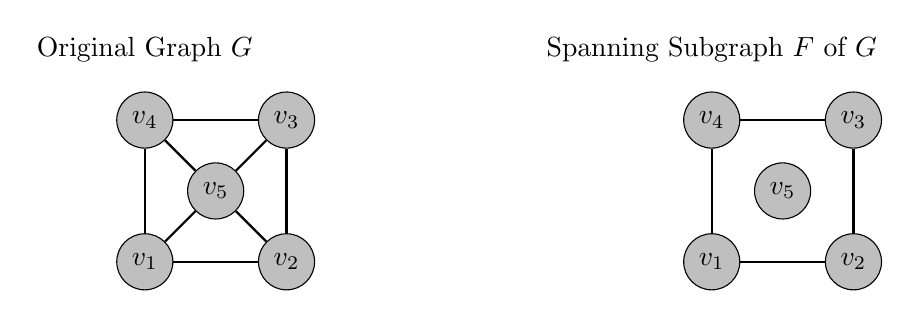
\begin{tikzpicture}[scale=0.9]
  % Original graph G
  \begin{scope}[shift={(-4,0)}]
    \node[align=center] at (0,3) {Original Graph $G$};
    
    % Vertices
    \node[draw, circle, fill=lightgray, minimum size=0.7cm] (v1) at (0,0) {$v_1$};
    \node[draw, circle, fill=lightgray, minimum size=0.7cm] (v2) at (2,0) {$v_2$};
    \node[draw, circle, fill=lightgray, minimum size=0.7cm] (v3) at (2,2) {$v_3$};
    \node[draw, circle, fill=lightgray, minimum size=0.7cm] (v4) at (0,2) {$v_4$};
    \node[draw, circle, fill=lightgray, minimum size=0.7cm] (v5) at (1,1) {$v_5$};
    
    % Edges
    \draw[thick] (v1) -- (v2);
    \draw[thick] (v2) -- (v3);
    \draw[thick] (v3) -- (v4);
    \draw[thick] (v4) -- (v1);
    \draw[thick] (v1) -- (v5);
    \draw[thick] (v2) -- (v5);
    \draw[thick] (v3) -- (v5);
    \draw[thick] (v4) -- (v5);
  \end{scope}
  
  % Spanning subgraph F
  \begin{scope}[shift={(4,0)}]
    \node[align=center] at (0,3) {Spanning Subgraph $F$ of $G$};
    
    % All vertices included (V(F) = V(G))
    \node[draw, circle, fill=lightgray, minimum size=0.7cm] (u1) at (0,0) {$v_1$};
    \node[draw, circle, fill=lightgray, minimum size=0.7cm] (u2) at (2,0) {$v_2$};
    \node[draw, circle, fill=lightgray, minimum size=0.7cm] (u3) at (2,2) {$v_3$};
    \node[draw, circle, fill=lightgray, minimum size=0.7cm] (u4) at (0,2) {$v_4$};
    \node[draw, circle, fill=lightgray, minimum size=0.7cm] (u5) at (1,1) {$v_5$};
    
    % Only some edges included (E(F) ⊆ E(G))
    \draw[thick] (u1) -- (u2);
    \draw[thick] (u2) -- (u3);
    \draw[thick] (u3) -- (u4);
    \draw[thick] (u4) -- (u1);
    % Edges connected to v5 are omitted
  \end{scope}
\end{tikzpicture}
\end{center}

% Caption
\vspace{0.3cm}
{\centering
\footnotesize Figure 17: Illustration of a spanning subgraph. The original graph $G$ (left) has 5 vertices and 8 edges, including connections from central vertex $v_5$ to all other vertices. The spanning subgraph $F$ (right) contains all vertices of $G$ but only a subset of edges, specifically removing all connections to the central vertex $v_5$. A spanning subgraph maintains the same vertex set as the original graph ($V(F) = V(G)$) but may have fewer edges ($E(F) \subseteq E(G)$).
\par}

\begin{definition}
If $X \subseteq V(G)$, the subgraph induced by $X$ is:
\begin{align*}
G[X] = (X, \{\{u,v\} \in E(G) : u, v \in X\})
\end{align*}
\end{definition}

\begin{center}
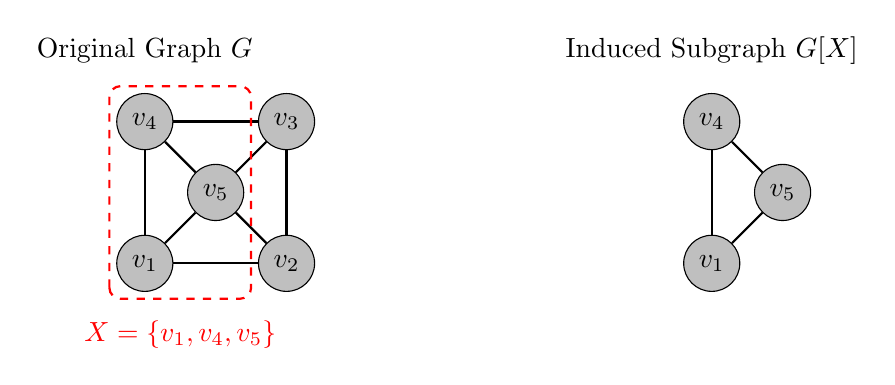
\begin{tikzpicture}[scale=0.9]
  % Original graph G
  \begin{scope}[shift={(-4,0)}]
    \node[align=center] at (0,3) {Original Graph $G$};
    
    % Vertices
    \node[draw, circle, fill=lightgray, minimum size=0.7cm] (v1) at (0,0) {$v_1$};
    \node[draw, circle, fill=lightgray, minimum size=0.7cm] (v2) at (2,0) {$v_2$};
    \node[draw, circle, fill=lightgray, minimum size=0.7cm] (v3) at (2,2) {$v_3$};
    \node[draw, circle, fill=lightgray, minimum size=0.7cm] (v4) at (0,2) {$v_4$};
    \node[draw, circle, fill=lightgray, minimum size=0.7cm] (v5) at (1,1) {$v_5$};
    
    % Edges
    \draw[thick] (v1) -- (v2);
    \draw[thick] (v2) -- (v3);
    \draw[thick] (v3) -- (v4);
    \draw[thick] (v4) -- (v1);
    \draw[thick] (v1) -- (v5);
    \draw[thick] (v2) -- (v5);
    \draw[thick] (v3) -- (v5);
    \draw[thick] (v4) -- (v5);
    
    % Highlight vertex set X for the induced subgraph
    \draw[dashed, rounded corners, red, thick] (-0.5,-0.5) rectangle (1.5,2.5);
    \node[red] at (0.5,-1) {$X = \{v_1, v_4, v_5\}$};
  \end{scope}
  
  % Induced subgraph G[X]
  \begin{scope}[shift={(4,0)}]
    \node[align=center] at (0,3) {Induced Subgraph $G[X]$};
    
    % Only vertices in X
    \node[draw, circle, fill=lightgray, minimum size=0.7cm] (u1) at (0,0) {$v_1$};
    \node[draw, circle, fill=lightgray, minimum size=0.7cm] (u4) at (0,2) {$v_4$};
    \node[draw, circle, fill=lightgray, minimum size=0.7cm] (u5) at (1,1) {$v_5$};
    
    % All original edges between vertices in X
    \draw[thick] (u1) -- (u4);
    \draw[thick] (u1) -- (u5);
    \draw[thick] (u4) -- (u5);
  \end{scope}
\end{tikzpicture}
\end{center}

% Caption
\vspace{0.3cm}
{\centering
\footnotesize Figure 18: Illustration of an induced subgraph. The original graph $G$ (left) has a subset of vertices $X = \{v_1, v_4, v_5\}$ highlighted by a red dashed rectangle. The induced subgraph $G[X]$ (right) contains exactly these vertices along with all edges from the original graph that connect vertices within this set. Unlike a general subgraph, an induced subgraph must include every edge from the original graph whose endpoints are both in the selected vertex subset.
\par}
\subsection{Walks and Paths in Graphs}
\begin{definition}
A walk in a graph is a sequence of vertices and edges:
\begin{align*}
v_0, \{v_0,v_1\}, v_1, \{v_1,v_2\}, v_2, \ldots, \{v_{k-1},v_k\}, v_k
\end{align*}
often abbreviated as $v_0, v_1, v_2, \ldots, v_k$.
The length of a walk is the number of edges in that walk.
\end{definition}
\begin{center}
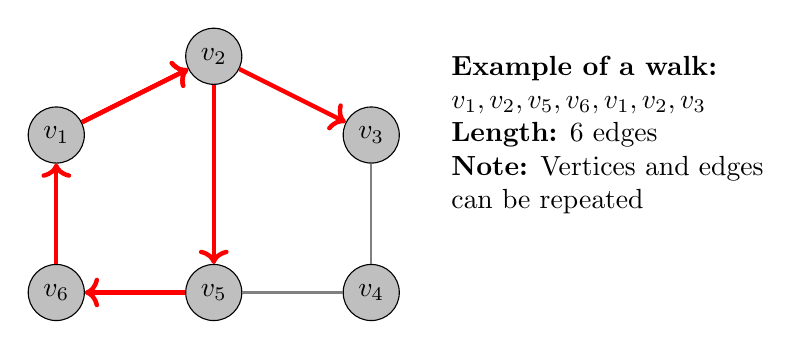
\begin{tikzpicture}[scale=1.0]
  % Basic graph
  \node[draw, circle, fill=lightgray, minimum size=0.7cm] (v1) at (0,0) {$v_1$};
  \node[draw, circle, fill=lightgray, minimum size=0.7cm] (v2) at (2,1) {$v_2$};
  \node[draw, circle, fill=lightgray, minimum size=0.7cm] (v3) at (4,0) {$v_3$};
  \node[draw, circle, fill=lightgray, minimum size=0.7cm] (v4) at (4,-2) {$v_4$};
  \node[draw, circle, fill=lightgray, minimum size=0.7cm] (v5) at (2,-2) {$v_5$};
  \node[draw, circle, fill=lightgray, minimum size=0.7cm] (v6) at (0,-2) {$v_6$};
  
  % All edges of the graph
  \draw[thick, gray] (v1) -- (v2);
  \draw[thick, gray] (v2) -- (v3);
  \draw[thick, gray] (v3) -- (v4);
  \draw[thick, gray] (v4) -- (v5);
  \draw[thick, gray] (v5) -- (v6);
  \draw[thick, gray] (v6) -- (v1);
  \draw[thick, gray] (v2) -- (v5);
  
  % Emphasize walk - can repeat vertices and edges
  \draw[->, ultra thick, red] (v1) -- (v2);
  \draw[->, ultra thick, red] (v2) -- (v5);
  \draw[->, ultra thick, red] (v5) -- (v6);
  \draw[->, ultra thick, red] (v6) -- (v1);
  \draw[->, ultra thick, red] (v1) -- (v2);
  \draw[->, ultra thick, red] (v2) -- (v3);
  
  % Walk description
  \node[align=left] at (7,0) {
    \textbf{Example of a walk:}\\
    $v_1, v_2, v_5, v_6, v_1, v_2, v_3$\\
    \textbf{Length:} 6 edges\\
    \textbf{Note:} Vertices and edges\\can be repeated
  };
\end{tikzpicture}
\end{center}

% Caption
\vspace{0.3cm}
{\centering
\footnotesize Figure 19: Illustration of a walk in graph theory. A walk is a sequence of vertices and edges where each consecutive pair of vertices in the sequence is connected by an edge. This example shows a walk of length 6 (red arrows) from $v_1$ to $v_3$ that passes through the sequence $v_1, v_2, v_5, v_6, v_1, v_2, v_3$. Unlike paths or trails, walks can repeat both vertices and edges. This walk repeats vertex $v_1$ and $v_2$, and also repeats the edge between them.
\par}
\begin{definition}
A path of length $k$ is a walk:
\begin{align*}
v_0, v_1, v_2, \ldots, v_k
\end{align*}
where all vertices are distinct.
\end{definition}
\begin{center}
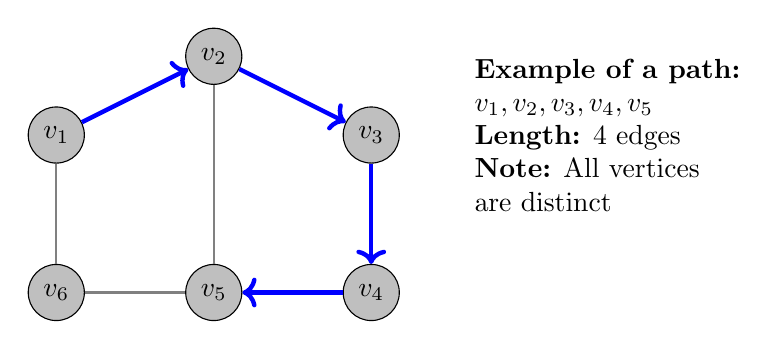
\begin{tikzpicture}[scale=1.0]
  % Basic graph
  \node[draw, circle, fill=lightgray, minimum size=0.7cm] (v1) at (0,0) {$v_1$};
  \node[draw, circle, fill=lightgray, minimum size=0.7cm] (v2) at (2,1) {$v_2$};
  \node[draw, circle, fill=lightgray, minimum size=0.7cm] (v3) at (4,0) {$v_3$};
  \node[draw, circle, fill=lightgray, minimum size=0.7cm] (v4) at (4,-2) {$v_4$};
  \node[draw, circle, fill=lightgray, minimum size=0.7cm] (v5) at (2,-2) {$v_5$};
  \node[draw, circle, fill=lightgray, minimum size=0.7cm] (v6) at (0,-2) {$v_6$};
  
  % All edges of the graph
  \draw[thick, gray] (v1) -- (v2);
  \draw[thick, gray] (v2) -- (v3);
  \draw[thick, gray] (v3) -- (v4);
  \draw[thick, gray] (v4) -- (v5);
  \draw[thick, gray] (v5) -- (v6);
  \draw[thick, gray] (v6) -- (v1);
  \draw[thick, gray] (v2) -- (v5);
  
  % Emphasize path - all vertices must be distinct
  \draw[->, ultra thick, blue] (v1) -- (v2);
  \draw[->, ultra thick, blue] (v2) -- (v3);
  \draw[->, ultra thick, blue] (v3) -- (v4);
  \draw[->, ultra thick, blue] (v4) -- (v5);
  
  % Path description
  \node[align=left] at (7,0) {
    \textbf{Example of a path:}\\
    $v_1, v_2, v_3, v_4, v_5$\\
    \textbf{Length:} 4 edges\\
    \textbf{Note:} All vertices\\are distinct
  };
\end{tikzpicture}
\end{center}

% Caption
\vspace{0.3cm}
{\centering
\footnotesize Figure 20: Illustration of a path in graph theory. A path is a walk where no vertex is repeated, ensuring each vertex appears at most once in the sequence. This example shows a path of length 4 (blue arrows) from $v_1$ to $v_5$ through the sequence $v_1, v_2, v_3, v_4, v_5$. Paths are fundamental structures in graph theory and are used to define important concepts such as connectivity, distance, and shortest paths between vertices. Unlike walks, the no-repetition constraint makes paths more restrictive but also more useful for many graph algorithms.
\par}

\begin{lemma}
A graph is connected if and only if every pair of vertices are the end of some walk.
\end{lemma}

\begin{definition}[Connected Graph]
A graph $G = (V, E)$ is said to be \textit{connected} if for every pair of distinct vertices $u, v \in V$, there exists a path in $G$ from $u$ to $v$. In other words, a graph is connected if and only if there is at least one path between any two vertices in the graph.
\end{definition}

\begin{definition}[Disconnected Graph]
A graph $G = (V, E)$ is said to be \textit{disconnected} if there exists at least one pair of distinct vertices $u, v \in V$ such that there is no path in $G$ from $u$ to $v$. Equivalently, a graph is disconnected if and only if its vertex set can be partitioned into two nonempty subsets such that there is no edge connecting any vertex in the first subset to any vertex in the second subset.
\end{definition}

\begin{definition}[Connected Component]
A \textit{connected component} of a graph $G = (V, E)$ is a maximal connected subgraph of $G$. That is, it is a connected subgraph $H = (V_H, E_H)$ of $G$ such that no larger connected subgraph of $G$ contains $H$ as a proper subgraph. A connected graph has exactly one connected component, while a disconnected graph has two or more connected components.
\end{definition}

\begin{center}
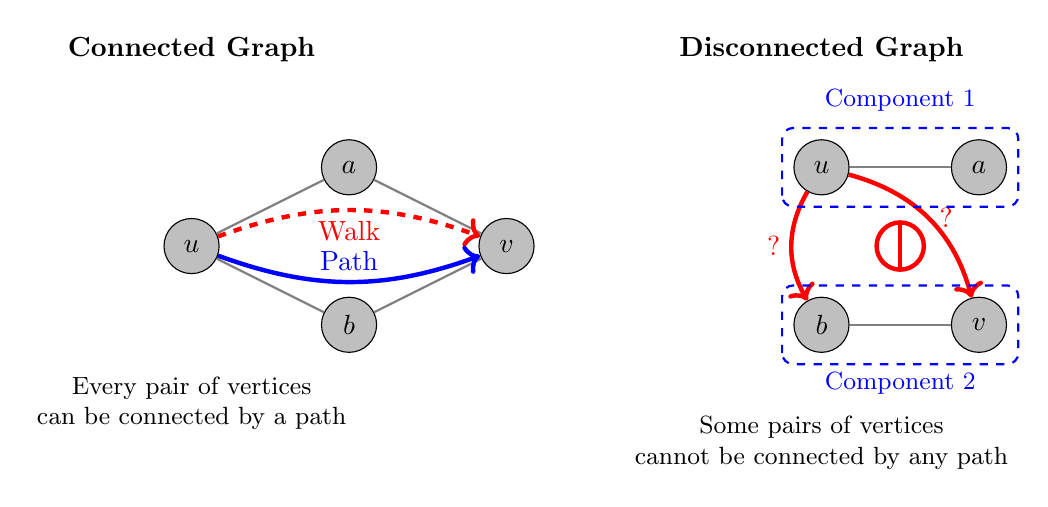
\begin{tikzpicture}[scale=1.0]
  \tikzset{
    vertex/.style={
      draw,
      circle,
      fill=lightgray,
      minimum size=0.7cm,
    },
    normaledge/.style={
      thick,
      gray,
    },
    walkpath/.style={
      ultra thick,
      red,
      dashed,
      ->,
    },
    simplepath/.style={
      ultra thick,
      blue,
      ->,
    },
    impossible/.style={
      ultra thick,
      red,
      ->,
    }
  }
  
  % Connected graph
  \begin{scope}[shift={(-4,0)}]
    \node[align=center, font=\bfseries] at (0,2.5) {Connected Graph};
    
    \node[vertex] (v1) at (0,0) {$u$};
    \node[vertex] (v2) at (2,1) {$a$};
    \node[vertex] (v3) at (2,-1) {$b$};
    \node[vertex] (v4) at (4,0) {$v$};
    
    % All edges
    \draw[normaledge] (v1) -- (v2);
    \draw[normaledge] (v1) -- (v3);
    \draw[normaledge] (v2) -- (v4);
    \draw[normaledge] (v3) -- (v4);
    
    % Walk and path
    \draw[walkpath] (v1) to[bend left=20] node[midway, below] {Walk } (v4);
    \draw[simplepath] (v1) to[bend right=20] node[midway, above] {Path} (v4);
    
    % Explanation
    \node[align=center, font=\small] at (0,-2) {
      Every pair of vertices\\can be connected by a path
    };
  \end{scope}
  
  % Disconnected graph
  \begin{scope}[shift={(4,0)}]
    \node[align=center, font=\bfseries] at (0,2.5) {Disconnected Graph};
    
    \node[vertex] (u1) at (0,1) {$u$};
    \node[vertex] (u2) at (2,1) {$a$};
    \node[vertex] (u3) at (0,-1) {$b$};
    \node[vertex] (u4) at (2,-1) {$v$};
    
    % All edges
    \draw[normaledge] (u1) -- (u2);
    \draw[normaledge] (u3) -- (u4);
    
    % Impossible paths
    \draw[impossible] (u1) to[bend right=30] node[midway, left] {?} (u3);
    \draw[impossible] (u1) to[bend left=30] node[midway, right] {?} (u4);
    \draw[red, ultra thick] (1,0) circle (0.3cm);
    \draw[red, ultra thick] (1,0.3) -- (1,-0.3);
    
    % Explanation
    \node[align=center, font=\small] at (0,-2.5) {
      Some pairs of vertices\\cannot be connected by any path
    };
    
    % Connected components highlight
    \draw[blue, dashed, rounded corners, thick] (-0.5,0.5) rectangle (2.5,1.5);
    \draw[blue, dashed, rounded corners, thick] (-0.5,-1.5) rectangle (2.5,-0.5);
    \node[blue, font=\small] at (1,1.85) {Component 1};
    \node[blue, font=\small] at (1,-1.75) {Component 2};
  \end{scope}
\end{tikzpicture}
\end{center}

% Caption for Figure 21
\vspace{0.3cm}
{\centering
\footnotesize Figure 21: Comparison of connected and disconnected graphs. In the connected graph (left), there exists at least one path between any pair of vertices, as shown by the example paths between vertices $u$ and $v$. The red dashed line represents one possible walk, while the blue solid line represents a path. In a disconnected graph (right), there exist pairs of vertices that cannot be connected by any path, as indicated by the crossed-out paths. The disconnected graph has two connected components (outlined in blue), which are maximal connected subgraphs.
\par}

\begin{proof}
Suppose vertices $u, v \in V(G)$ are the ends of a walk:
\begin{align*}
u = v_0, v_1, \ldots, v_k = v
\end{align*}
Take a shortest walk from $u$ to $v$. We can cut out any loops in the walk.
If some $v_i$ is visited more than once, say:
\begin{align*}
u \to v_i \to \ldots \to v_i \to v
\end{align*}
Then we can use the segment of the walk from $u$ to $v_i$ followed by the segment from $v_i$ to $v$:
\begin{align*}
u \to v_i \to v
\end{align*}
which is shorter, a contradiction.
So a shortest walk from $u$ to $v$ is a path.
\end{proof}

\begin{center}
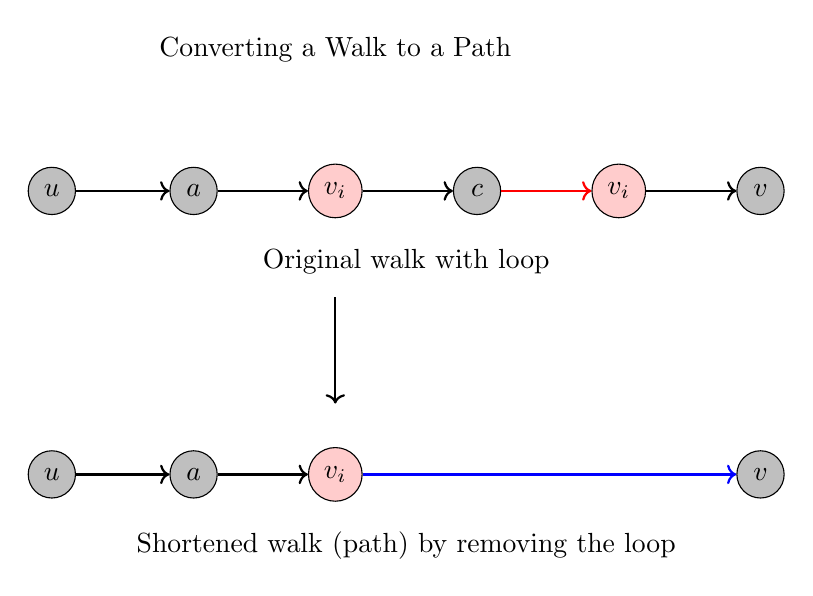
\begin{tikzpicture}[scale=0.9]
  % Proof diagram
  \node[align=center] at (0,3) {Converting a Walk to a Path};
  
  % Original walk (with loop)
  \begin{scope}[shift={(0,1)}]
    \node[draw, circle, fill=lightgray, minimum size=0.6cm] (u) at (-4,0) {$u$};
    \node[draw, circle, fill=lightgray, minimum size=0.6cm] (a) at (-2,0) {$a$};
    \node[draw, circle, fill=red!20, minimum size=0.6cm] (b) at (0,0) {$v_i$};
    \node[draw, circle, fill=lightgray, minimum size=0.6cm] (c) at (2,0) {$c$};
    \node[draw, circle, fill=red!20, minimum size=0.6cm] (b2) at (4,0) {$v_i$};
    \node[draw, circle, fill=lightgray, minimum size=0.6cm] (v) at (6,0) {$v$};
    
    \draw[->, thick] (u) -- (a);
    \draw[->, thick] (a) -- (b);
    \draw[->, thick] (b) -- (c);
    \draw[->, thick, red] (c) -- (b2);
    \draw[->, thick] (b2) -- (v);
    
    \node[align=center] at (1,-1) {Original walk with loop};
  \end{scope}
  
  \draw[->, thick] (0,-0.5) -- (0,-2);
  
  % Shortened walk (path)
  \begin{scope}[shift={(0,-3)}]
    \node[draw, circle, fill=lightgray, minimum size=0.6cm] (u) at (-4,0) {$u$};
    \node[draw, circle, fill=lightgray, minimum size=0.6cm] (a) at (-2,0) {$a$};
    \node[draw, circle, fill=red!20, minimum size=0.6cm] (b) at (0,0) {$v_i$};
    \node[draw, circle, fill=lightgray, minimum size=0.6cm] (v) at (6,0) {$v$};
    
    \draw[->, thick] (u) -- (a);
    \draw[->, thick] (a) -- (b);
    \draw[->, thick, blue] (b) -- (v);
    
    \node[align=center] at (1,-1) {Shortened walk (path) by removing the loop};
  \end{scope}
\end{tikzpicture}
\end{center}

% Caption
\vspace{0.3cm}
{\centering
\footnotesize Figure 22: Illustration of the process of converting a walk to a path by removing loops. In the original walk (top), vertex $v_i$ appears twice, creating a loop in the walk. By removing the portion of the walk between the two occurrences of $v_i$ (marked in red), we obtain a shorter walk from $u$ to $v$ that doesn't repeat any vertices (bottom), thus forming a path. This technique is fundamental for proving that if there exists a walk between two vertices in a graph, then there must also exist a path between them.
\par}

\subsubsection{More Examples of Walks, Paths, and Components}
\begin{center}
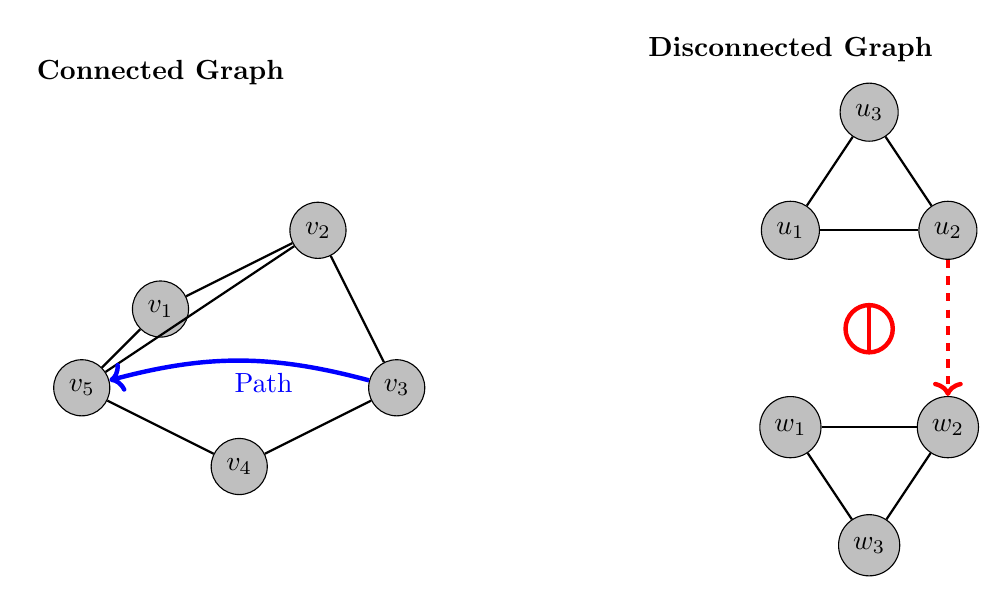
\begin{tikzpicture}[scale=1.0]
  % Connected graph
  \begin{scope}[shift={(-4,0)}]
    \node[align=center,font=\bfseries] at (0,3) {Connected Graph};
    
    % Vertices
    \node[draw, circle, fill=lightgray, minimum size=0.7cm] (v1) at (0,0) {$v_1$};
    \node[draw, circle, fill=lightgray, minimum size=0.7cm] (v2) at (2,1) {$v_2$};
    \node[draw, circle, fill=lightgray, minimum size=0.7cm] (v3) at (3,-1) {$v_3$};
    \node[draw, circle, fill=lightgray, minimum size=0.7cm] (v4) at (1,-2) {$v_4$};
    \node[draw, circle, fill=lightgray, minimum size=0.7cm] (v5) at (-1,-1) {$v_5$};
    
    % Edges
    \draw[thick] (v1) -- (v2);
    \draw[thick] (v2) -- (v3);
    \draw[thick] (v3) -- (v4);
    \draw[thick] (v4) -- (v5);
    \draw[thick] (v5) -- (v1);
    \draw[thick] (v2) -- (v5);
    
    % Highlight a path between arbitrary vertices
    \draw[->, ultra thick, blue] (v3) to[bend right=15] node[pos=0.4, below] {Path} (v5);
  \end{scope}
  
  % Disconnected graph
  \begin{scope}[shift={(4,0)}]
    \node[align=center,font=\bfseries] at (0,3.3) {Disconnected Graph};
    
    % First component
    \node[draw, circle, fill=lightgray, minimum size=0.7cm] (u1) at (0,1) {$u_1$};
    \node[draw, circle, fill=lightgray, minimum size=0.7cm] (u2) at (2,1) {$u_2$};
    \node[draw, circle, fill=lightgray, minimum size=0.7cm] (u3) at (1,2.5) {$u_3$};
    
    % Second component
    \node[draw, circle, fill=lightgray, minimum size=0.7cm] (w1) at (0,-1.5) {$w_1$};
    \node[draw, circle, fill=lightgray, minimum size=0.7cm] (w2) at (2,-1.5) {$w_2$};
    \node[draw, circle, fill=lightgray, minimum size=0.7cm] (w3) at (1,-3) {$w_3$};
    
    % Edges
    \draw[thick] (u1) -- (u2);
    \draw[thick] (u2) -- (u3);
    \draw[thick] (u3) -- (u1);
    
    \draw[thick] (w1) -- (w2);
    \draw[thick] (w2) -- (w3);
    \draw[thick] (w3) -- (w1);
    
    % Impossible path indicator
    \draw[->, ultra thick, red, dashed] (u2) -- (w2);
    \draw[red, ultra thick] (1,-0.25) circle (0.3cm);
    \draw[red, ultra thick] (1,0.05) -- (1,-0.55);
  \end{scope}
\end{tikzpicture}
\end{center}

% Caption
\vspace{0.3cm}
{\centering
\footnotesize Figure 23: Comparison of connected and disconnected graphs. The connected graph (left) has a single component where a path exists between any pair of vertices, demonstrated by the blue path from $v_3$ to $v_5$. The disconnected graph (right) contains two triangular structures that have no paths between them, as shown by the crossed-out red line. This fundamental distinction affects many graph properties, including traversability, algorithmic complexity, and network reliability.
\par}

\begin{center}
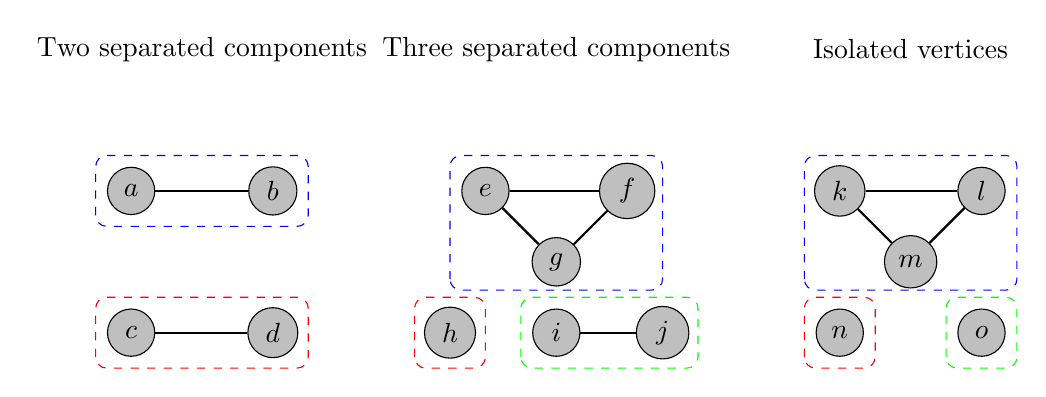
\begin{tikzpicture}[scale=0.9]
  % Various examples of disconnected graphs
  
  % Example 1: Two separated components
  \begin{scope}[shift={(-5,0)}]
    \node[align=center] at (0,3) {Two separated components};
    
    % First component
    \node[draw, circle, fill=lightgray, minimum size=0.6cm] (a1) at (-1,1) {$a$};
    \node[draw, circle, fill=lightgray, minimum size=0.6cm] (a2) at (1,1) {$b$};
    \draw[thick] (a1) -- (a2);
    
    % Second component
    \node[draw, circle, fill=lightgray, minimum size=0.6cm] (a3) at (-1,-1) {$c$};
    \node[draw, circle, fill=lightgray, minimum size=0.6cm] (a4) at (1,-1) {$d$};
    \draw[thick] (a3) -- (a4);
    
    % Component distinction
    \draw[blue, dashed, rounded corners] (-1.5,0.5) rectangle (1.5,1.5);
    \draw[red, dashed, rounded corners] (-1.5,-1.5) rectangle (1.5,-0.5);
  \end{scope}
  
  % Example 2: Three separated components
  \begin{scope}[shift={(0,0)}]
    \node[align=center] at (0,3) {Three separated components};
    
    % First component (triangle)
    \node[draw, circle, fill=lightgray, minimum size=0.6cm] (b1) at (-1,1) {$e$};
    \node[draw, circle, fill=lightgray, minimum size=0.6cm] (b2) at (1,1) {$f$};
    \node[draw, circle, fill=lightgray, minimum size=0.6cm] (b3) at (0,0) {$g$};
    \draw[thick] (b1) -- (b2);
    \draw[thick] (b2) -- (b3);
    \draw[thick] (b3) -- (b1);
    
    % Second component (single vertex)
    \node[draw, circle, fill=lightgray, minimum size=0.6cm] (b4) at (-1.5,-1) {$h$};
    
    % Third component (line)
    \node[draw, circle, fill=lightgray, minimum size=0.6cm] (b5) at (0,-1) {$i$};
    \node[draw, circle, fill=lightgray, minimum size=0.6cm] (b6) at (1.5,-1) {$j$};
    \draw[thick] (b5) -- (b6);
    
    % Component distinction
    \draw[blue, dashed, rounded corners] (-1.5,-0.4) rectangle (1.5,1.5);
    \draw[red, dashed, rounded corners] (-2,-1.5) rectangle (-1,-0.5);
    \draw[green, dashed, rounded corners] (-0.5,-1.5) rectangle (2,-0.5);
  \end{scope}
  
  % Example 3: Case with isolated vertices
  \begin{scope}[shift={(5,0)}]
    \node[align=center] at (0,3) {Isolated vertices};
    
    % Main component
    \node[draw, circle, fill=lightgray, minimum size=0.6cm] (c1) at (-1,1) {$k$};
    \node[draw, circle, fill=lightgray, minimum size=0.6cm] (c2) at (1,1) {$l$};
    \node[draw, circle, fill=lightgray, minimum size=0.6cm] (c3) at (0,0) {$m$};
    \draw[thick] (c1) -- (c2);
    \draw[thick] (c2) -- (c3);
    \draw[thick] (c3) -- (c1);
    
    % Isolated vertices
    \node[draw, circle, fill=lightgray, minimum size=0.6cm] (c4) at (-1,-1) {$n$};
    \node[draw, circle, fill=lightgray, minimum size=0.6cm] (c5) at (1,-1) {$o$};
    
    % Component distinction
    \draw[blue, dashed, rounded corners] (-1.5,-0.4) rectangle (1.5,1.5);
    \draw[red, dashed, rounded corners] (-1.5,-1.5) rectangle (-0.5,-0.5);
    \draw[green, dashed, rounded corners] (0.5,-1.5) rectangle (1.5,-0.5);
  \end{scope}
\end{tikzpicture}
\end{center}

% Caption
\vspace{0.3cm}
{\centering
\footnotesize Figure 24: Various forms of disconnected graphs. Left: A disconnected graph with two separate edge components, where each component is a single edge. Middle: A graph with three distinct components - a triangular component, a single isolated vertex, and a path component with two vertices. Right: A graph with a triangular component and two isolated vertices. Each connected component (highlighted by dashed colored rectangles) forms a maximal connected subgraph. In graph theory, isolated vertices are considered separate connected components.
\par}

\begin{center}
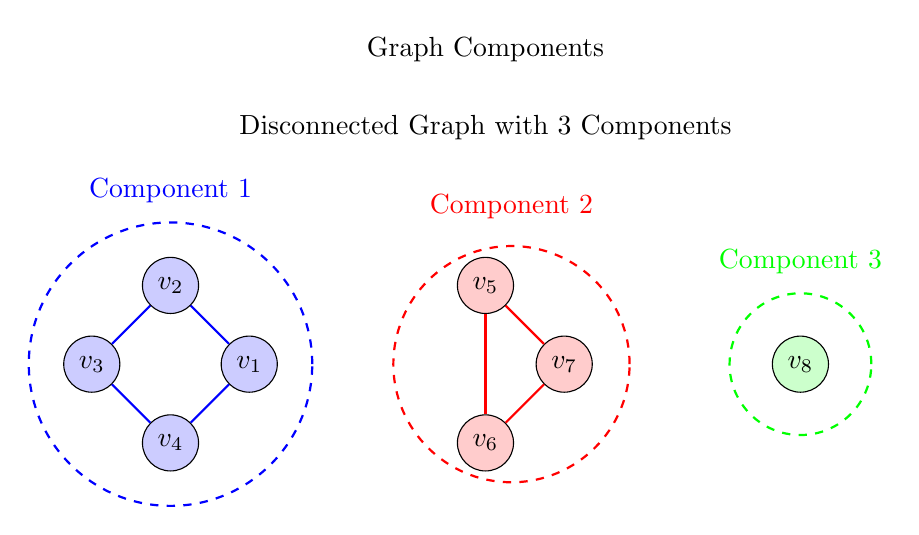
\begin{tikzpicture}[scale=1.0]
  % Disconnected graph and its components
  \node[align=center] at (0,4) {Graph Components};
  
  % Original disconnected graph
  \begin{scope}
    \node[align=center] at (0,3) {Disconnected Graph with 3 Components};
    
    % First component
    \node[draw, circle, fill=blue!20, minimum size=0.7cm] (v1) at (-3,0) {$v_1$};
    \node[draw, circle, fill=blue!20, minimum size=0.7cm] (v2) at (-4,1) {$v_2$};
    \node[draw, circle, fill=blue!20, minimum size=0.7cm] (v3) at (-5,0) {$v_3$};
    \node[draw, circle, fill=blue!20, minimum size=0.7cm] (v4) at (-4,-1) {$v_4$};
    
    % First component edges
    \draw[thick, blue] (v1) -- (v2);
    \draw[thick, blue] (v2) -- (v3);
    \draw[thick, blue] (v3) -- (v4);
    \draw[thick, blue] (v4) -- (v1);
    
    % Second component
    \node[draw, circle, fill=red!20, minimum size=0.7cm] (v5) at (0,1) {$v_5$};
    \node[draw, circle, fill=red!20, minimum size=0.7cm] (v6) at (0,-1) {$v_6$};
    \node[draw, circle, fill=red!20, minimum size=0.7cm] (v7) at (1,0) {$v_7$};
    
    % Second component edges
    \draw[thick, red] (v5) -- (v6);
    \draw[thick, red] (v6) -- (v7);
    \draw[thick, red] (v7) -- (v5);
    
    % Third component (single vertex)
    \node[draw, circle, fill=green!20, minimum size=0.7cm] (v8) at (4,0) {$v_8$};
    
    % Component emphasis (dashed circles)
    \draw[blue, dashed, thick] (-4,0) circle (1.8cm);
    \draw[red, dashed, thick] (0.33,0) circle (1.5cm);
    \draw[green, dashed, thick] (4,0) circle (0.9cm);
    
    % Component labels - positioned to avoid overlap
    \node[blue] at (-4,2.2) {Component 1};
    \node[red] at (0.33,2) {Component 2};
    \node[green] at (4,1.3) {Component 3};
  \end{scope}
\end{tikzpicture}
\end{center}

% Caption
\vspace{0.3cm}
{\centering
\footnotesize Figure 25: Illustration of a disconnected graph with three distinct components. Component 1 (blue) is a cycle graph with 4 vertices. Component 2 (red) is a triangle with 3 vertices. Component 3 (green) consists of a single isolated vertex. Each component is a maximal connected subgraph, meaning that there exists a path between any two vertices within the same component, but no path between vertices from different components. The number of components in a graph is an important invariant that affects connectivity, traversability, and many graph algorithms.
\par}

\newpage
\subsection{Chapter 1 Exercises}

\subsubsection{Easy Questions}

\begin{enumerate}
\item Define the degree of a vertex in a graph and calculate the sum of all vertex degrees in the cycle graph $C_5$.

\item Draw all possible non-isomorphic simple graphs with exactly 3 vertices.

\item Consider the following graph:
\begin{center}
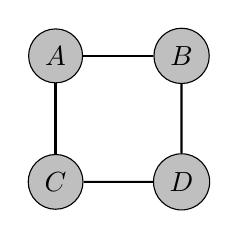
\begin{tikzpicture}[scale=0.8]
    \node[draw, circle, fill=lightgray, minimum size=0.6cm] (A) at (0,0) {$A$};
    \node[draw, circle, fill=lightgray, minimum size=0.6cm] (B) at (2,0) {$B$};
    \node[draw, circle, fill=lightgray, minimum size=0.6cm] (C) at (0,-2) {$C$};
    \node[draw, circle, fill=lightgray, minimum size=0.6cm] (D) at (2,-2) {$D$};
    
    \draw[thick] (A) -- (B);
    \draw[thick] (A) -- (C);
    \draw[thick] (B) -- (D);
    \draw[thick] (C) -- (D);
\end{tikzpicture}
\end{center}
List all paths from vertex $A$ to vertex $D$.

\item What is the difference between a walk and a path in a graph? Give an example of a walk that is not a path.

\item For each of the following graphs, determine if it is connected or disconnected:
\begin{itemize}
    \item A star graph $S_6$
    \item A path graph $P_4$
    \item A graph with vertices $\{a,b,c,d\}$ and edges $\{\{a,b\}, \{c,d\}\}$
\end{itemize}
\end{enumerate}

\subsubsection{Intermediate Questions}

\begin{enumerate}[resume]
\item Draw a graph with degree sequence $(3,3,2,2,2,0)$. Is there more than one non-isomorphic graph with this degree sequence?

\item Prove that a connected graph with $n$ vertices must have at least $n-1$ edges.

\item Consider a graph $G$ with vertex set $V = \{1,2,3,4,5,6\}$ and edges 
$\{1,2\}$, $\{1,5\}$, $\{2,3\}$, $\{2,5\}$,\\
$\{3,4\}$, $\{4,5\}$, $\{4,6\}$, $\{5,6\}$.
\begin{center}
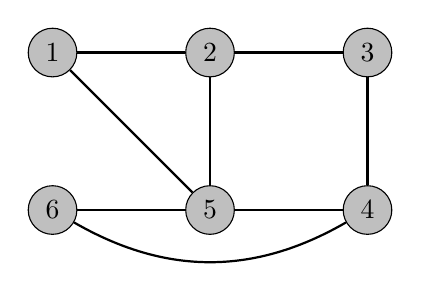
\begin{tikzpicture}[scale=1.0]
    \node[draw, circle, fill=lightgray, minimum size=0.6cm] (1) at (0,0) {$1$};
    \node[draw, circle, fill=lightgray, minimum size=0.6cm] (2) at (2,0) {$2$};
    \node[draw, circle, fill=lightgray, minimum size=0.6cm] (3) at (4,0) {$3$};
    \node[draw, circle, fill=lightgray, minimum size=0.6cm] (4) at (4,-2) {$4$};
    \node[draw, circle, fill=lightgray, minimum size=0.6cm] (5) at (2,-2) {$5$};
    \node[draw, circle, fill=lightgray, minimum size=0.6cm] (6) at (0,-2) {$6$};
    
    \draw[thick] (1) -- (2);
    \draw[thick] (1) -- (5);
    \draw[thick] (2) -- (3);
    \draw[thick] (2) -- (5);
    \draw[thick] (3) -- (4);
    \draw[thick] (4) -- (5);
    \draw[thick] (4) to[bend left=30] (6); % Bent edge to avoid confusion
    \draw[thick] (5) -- (6);
\end{tikzpicture}
\end{center}
\begin{itemize}
    \item Find an induced subgraph with vertex set $\{1,2,5,6\}$
    \item Find a spanning subgraph with exactly 6 edges
\end{itemize}

\item The Petersen graph is shown in your textbook (Figure 11). Find the longest path in this graph. Prove that your path is indeed the longest possible.

\item Show that any graph with at least two vertices must have at least two vertices with the same degree.

\end{enumerate}

\subsubsection{Hard Questions}

\begin{enumerate}[resume]
\item Prove that if $G$ is a simple graph with $n$ vertices and more than $\frac{(n-1)(n-2)}{2}$ edges, then $G$ must be connected.

\item Let $G$ be a graph with $n$ vertices. If each vertex has degree at least $\frac{n-1}{2}$, prove that $G$ is connected.

\item A graph is called bipartite if its vertices can be divided into two disjoint sets such that every edge connects a vertex in the first set to one in the second set.
\begin{itemize}
    \item Prove that a graph is bipartite if and only if it contains no cycles of odd length.
    \item Which of the following graphs are bipartite: $C_4$, $C_5$, $K_{3,3}$, the Petersen graph?
\end{itemize}

\item Design a graph that:
\begin{itemize}
    \item Has exactly 8 vertices
    \item Is connected
    \item Has exactly 3 vertices of degree 3, and the rest of degree 2
    \item Contains exactly one cycle of length 4 and one cycle of length 5
\end{itemize}

\item Consider the hypercube graph $Q_4$.
\begin{itemize}
    \item How many vertices and edges does $Q_4$ have?
    \item What is the degree of each vertex?
    \item Devise an algorithm to determine if there exists a path of length exactly $k$ between any two vertices in $Q_4$.
\end{itemize}
\end{enumerate}

\subsubsection{Questions with Diagrams}

\begin{enumerate}[resume]
\item For the graph below, identify:
\begin{itemize}
    \item All isolated vertices
    \item All pendant vertices
    \item The degree sequence
    \item The number of connected components
\end{itemize}

\begin{center}
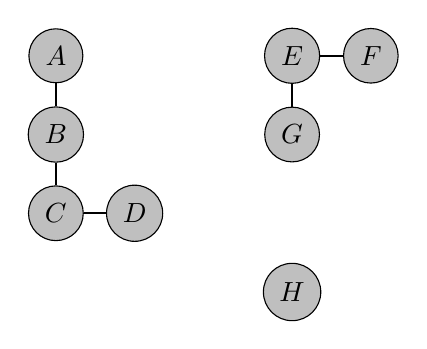
\begin{tikzpicture}[scale=1.0]
    \node[draw, circle, fill=lightgray, minimum size=0.6cm] (A) at (0,0) {$A$};
    \node[draw, circle, fill=lightgray, minimum size=0.6cm] (B) at (0,-1) {$B$};
    \node[draw, circle, fill=lightgray, minimum size=0.6cm] (C) at (0,-2) {$C$};
    \node[draw, circle, fill=lightgray, minimum size=0.6cm] (D) at (1,-2) {$D$};
    \node[draw, circle, fill=lightgray, minimum size=0.6cm] (E) at (3,0) {$E$};
    \node[draw, circle, fill=lightgray, minimum size=0.6cm] (F) at (4,0) {$F$};
    \node[draw, circle, fill=lightgray, minimum size=0.6cm] (G) at (3,-1) {$G$};
    \node[draw, circle, fill=lightgray, minimum size=0.6cm] (H) at (3,-3) {$H$};
    
    \draw[thick] (A) -- (B);
    \draw[thick] (B) -- (C);
    \draw[thick] (C) -- (D);
    \draw[thick] (E) -- (F);
    \draw[thick] (E) -- (G);
\end{tikzpicture}
\end{center}

\item Draw all possible spanning trees of the following graph:
(Hint 1: Refer to Definition 33 in Chapter 5-2, pg 63)

\begin{center}
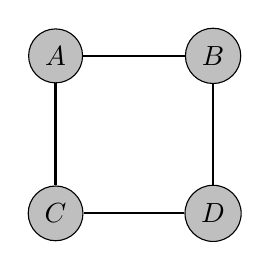
\begin{tikzpicture}[scale=1.0]
    \node[draw, circle, fill=lightgray, minimum size=0.6cm] (A) at (0,0) {$A$};
    \node[draw, circle, fill=lightgray, minimum size=0.6cm] (B) at (2,0) {$B$};
    \node[draw, circle, fill=lightgray, minimum size=0.6cm] (C) at (0,-2) {$C$};
    \node[draw, circle, fill=lightgray, minimum size=0.6cm] (D) at (2,-2) {$D$};
    
    \draw[thick] (A) -- (B);
    \draw[thick] (A) -- (C);
    \draw[thick] (B) -- (D);
    \draw[thick] (C) -- (D);
\end{tikzpicture}
\end{center}

\item Consider the graph $G$ shown below:

\begin{center}
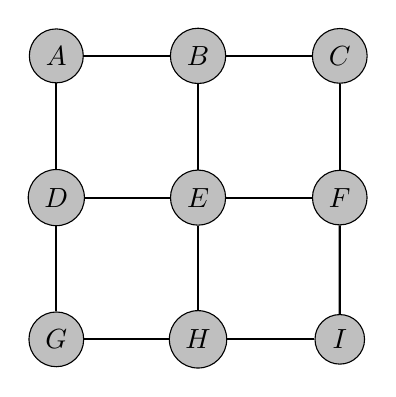
\begin{tikzpicture}[scale=0.9]
    \node[draw, circle, fill=lightgray, minimum size=0.6cm] (A) at (0,0) {$A$};
    \node[draw, circle, fill=lightgray, minimum size=0.6cm] (B) at (2,0) {$B$};
    \node[draw, circle, fill=lightgray, minimum size=0.6cm] (C) at (4,0) {$C$};
    \node[draw, circle, fill=lightgray, minimum size=0.6cm] (D) at (0,-2) {$D$};
    \node[draw, circle, fill=lightgray, minimum size=0.6cm] (E) at (2,-2) {$E$};
    \node[draw, circle, fill=lightgray, minimum size=0.6cm] (F) at (4,-2) {$F$};
    \node[draw, circle, fill=lightgray, minimum size=0.6cm] (G) at (0,-4) {$G$};
    \node[draw, circle, fill=lightgray, minimum size=0.6cm] (H) at (2,-4) {$H$};
    \node[draw, circle, fill=lightgray, minimum size=0.6cm] (I) at (4,-4) {$I$};
    
    \draw[thick] (A) -- (B);
    \draw[thick] (B) -- (C);
    \draw[thick] (A) -- (D);
    \draw[thick] (B) -- (E);
    \draw[thick] (C) -- (F);
    \draw[thick] (D) -- (E);
    \draw[thick] (E) -- (F);
    \draw[thick] (D) -- (G);
    \draw[thick] (E) -- (H);
    \draw[thick] (F) -- (I);
    \draw[thick] (G) -- (H);
    \draw[thick] (H) -- (I);
\end{tikzpicture}
\end{center}

\begin{enumerate}[label=\alph*)]
    \item Draw an induced subgraph $G[\{A,B,D,E\}]$
    \item Find a subgraph that is not an induced subgraph
    \item Draw a spanning subgraph that is a tree
    \item What is the maximum number of edges that can be removed while keeping the graph connected?
\end{enumerate}

\item In the wheel graph $W_6$ (shown below), find:
\begin{itemize}
    \item The shortest path from any outer vertex to the vertex diametrically opposite on the cycle
    \item The number of distinct cycles of length 3
    \item The number of distinct cycles of length 4
\end{itemize}

\begin{center}
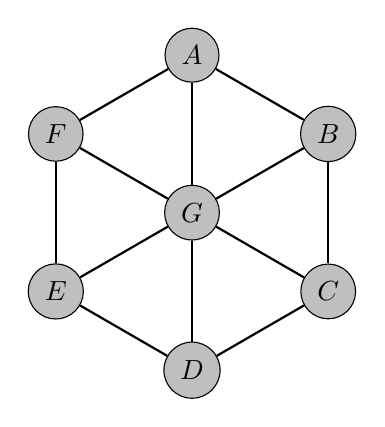
\begin{tikzpicture}[scale=1.0]
    \node[draw, circle, fill=lightgray, minimum size=0.6cm] (G) at (0,0) {$G$};
    \node[draw, circle, fill=lightgray, minimum size=0.6cm] (A) at (0,2) {$A$};
    \node[draw, circle, fill=lightgray, minimum size=0.6cm] (B) at (1.73,1) {$B$};
    \node[draw, circle, fill=lightgray, minimum size=0.6cm] (C) at (1.73,-1) {$C$};
    \node[draw, circle, fill=lightgray, minimum size=0.6cm] (D) at (0,-2) {$D$};
    \node[draw, circle, fill=lightgray, minimum size=0.6cm] (E) at (-1.73,-1) {$E$};
    \node[draw, circle, fill=lightgray, minimum size=0.6cm] (F) at (-1.73,1) {$F$};
    
    \draw[thick] (A) -- (B);
    \draw[thick] (B) -- (C);
    \draw[thick] (C) -- (D);
    \draw[thick] (D) -- (E);
    \draw[thick] (E) -- (F);
    \draw[thick] (F) -- (A);
    
    \draw[thick] (G) -- (A);
    \draw[thick] (G) -- (B);
    \draw[thick] (G) -- (C);
    \draw[thick] (G) -- (D);
    \draw[thick] (G) -- (E);
    \draw[thick] (G) -- (F);
\end{tikzpicture}
\end{center}

\item Given the Petersen graph:
\begin{center}
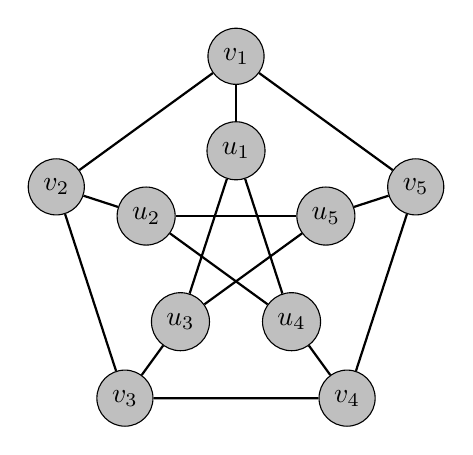
\begin{tikzpicture}[scale=1.2]
  % Outer pentagon
  \foreach \i in {1,...,5} {
    \node[draw, circle, fill=lightgray, minimum size=0.6cm] (v\i) at ({72*(\i-1)+90}:2) {$v_{\i}$};
  }
  
  % Inner pentagon
  \foreach \i in {1,...,5} {
    \node[draw, circle, fill=lightgray, minimum size=0.6cm] (u\i) at ({72*(\i-1)+90}:1) {$u_{\i}$};
  }
  
  % Connect outer pentagon
  \foreach \i in {1,...,5} {
    \pgfmathtruncatemacro{\j}{mod(\i,5)+1}
    \draw[thick] (v\i) -- (v\j);
  }
  
  % Connect inner to outer
  \foreach \i in {1,...,5} {
    \draw[thick] (v\i) -- (u\i);
  }
  
  % Connect inner pentagon in star pattern
  \foreach \i in {1,...,5} {
    \pgfmathtruncatemacro{\j}{mod(\i+1,5)+1}
    \draw[thick] (u\i) -- (u\j);
  }
\end{tikzpicture}
\end{center}

\begin{enumerate}[label=\alph*)]
    \item Prove that it does not contain a cycle of length 3
    \item Find all cycles of length 5
    \item Show that the graph is not bipartite (Hint : Chapter 5-9)
\end{enumerate}

\end{enumerate}


\section{Eulerian Graphs}

\subsection{Trails and Tours}

\begin{definition}
A trail in a graph is a sequence of vertices:
\begin{align*}
v_1, v_2, \ldots, v_n
\end{align*}
such that $\{v_i, v_{i+1}\} \in E(G)$ and no edge appears twice. Unlike a path, a trail may visit the same vertex multiple times, but it cannot use the same edge more than once.
\end{definition}

\begin{definition}
A tour is a trail $v_1, v_2, \ldots, v_n$ with $v_n = v_1$. That is, a tour is a closed trail that starts and ends at the same vertex. A tour is also sometimes called a circuit.
\end{definition}

\begin{definition}
An Eulerian trail is a trail that traverses every edge of the graph exactly once.
\end{definition}

\begin{definition}
An Eulerian tour (or Eulerian circuit) is a tour that traverses every edge of the graph exactly once.
\end{definition}

\begin{theorem}
Let $G$ be a connected graph (or multigraph), and let $u, v \in V(G)$. Then:
\begin{enumerate}
\item The graph has an Eulerian tour if and only if all vertices have even degree.
\item The graph has an Eulerian trail from $u$ to $v$ if and only if $u$ and $v$ have odd degree and all other vertices have even degree.
\end{enumerate}
\end{theorem}

\begin{figure}[ht]
\centering
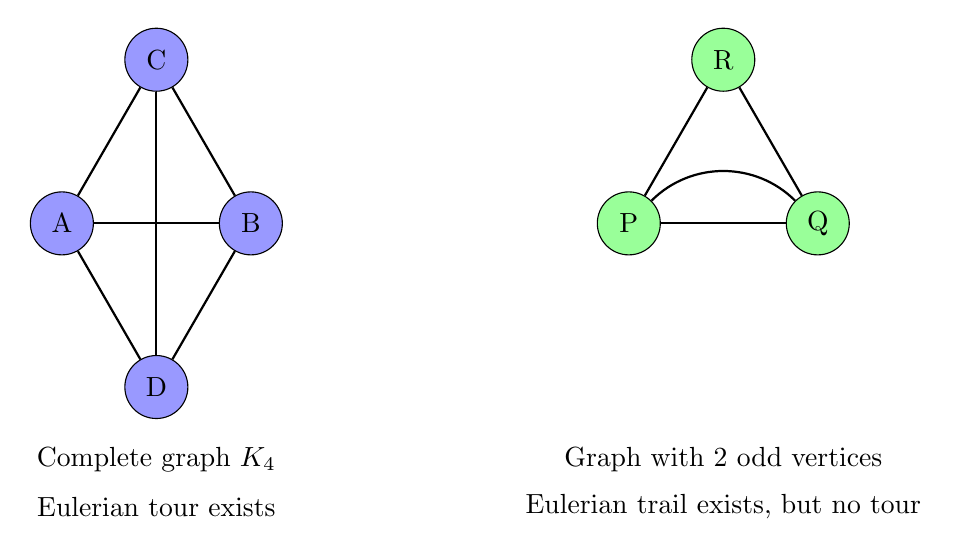
\begin{tikzpicture}[scale=1.2]
    % Example 1: Graph with Eulerian Tour
    \begin{scope}[shift={(-3,0)}]
        % Vertices
        \node[circle, draw, fill=blue!40, minimum size=0.8cm] (A) at (0,0) {A};
        \node[circle, draw, fill=blue!40, minimum size=0.8cm] (B) at (2,0) {B};
        \node[circle, draw, fill=blue!40, minimum size=0.8cm] (C) at (1,1.732) {C};
        \node[circle, draw, fill=blue!40, minimum size=0.8cm] (D) at (1,-1.732) {D};
        
        % Edges
        \draw[thick] (A) -- (B);
        \draw[thick] (A) -- (C);
        \draw[thick] (A) -- (D);
        \draw[thick] (B) -- (C);
        \draw[thick] (B) -- (D);
        \draw[thick] (C) -- (D);
        
        \node at (1,-2.5) {Complete graph $K_4$};
        \node at (1,-3) {Eulerian tour exists};
    \end{scope}
    
    % Example 2: Graph with Eulerian Trail but no Tour
    \begin{scope}[shift={(3,0)}]
        % Vertices
        \node[circle, draw, fill=green!40, minimum size=0.8cm] (P) at (0,0) {P};
        \node[circle, draw, fill=green!40, minimum size=0.8cm] (Q) at (2,0) {Q};
        \node[circle, draw, fill=green!40, minimum size=0.8cm] (R) at (1,1.732) {R};
        
        % Edges
        \draw[thick] (P) -- (Q);
        \draw[thick] (P) -- (R);
        \draw[thick] (Q) -- (R);
        \draw[thick] (P) to[bend left=45] (Q);
        
        \node at (1,-2.5) {Graph with 2 odd vertices};
        \node at (1,-3) {Eulerian trail exists, but no tour};
    \end{scope}
\end{tikzpicture}

\vspace{0.3cm}
{\centering
\small Figure 26: Example graphs illustrating Eulerian concepts. Left: Complete graph $K_4$ where all vertices have degree 3 (odd). Although it doesn't have an Eulerian tour, it does have an Eulerian trail. Right: A graph with exactly two odd-degree vertices (P and Q) that has an Eulerian trail but no Eulerian tour.
\par}
\end{figure}

\begin{figure}[ht]
\centering
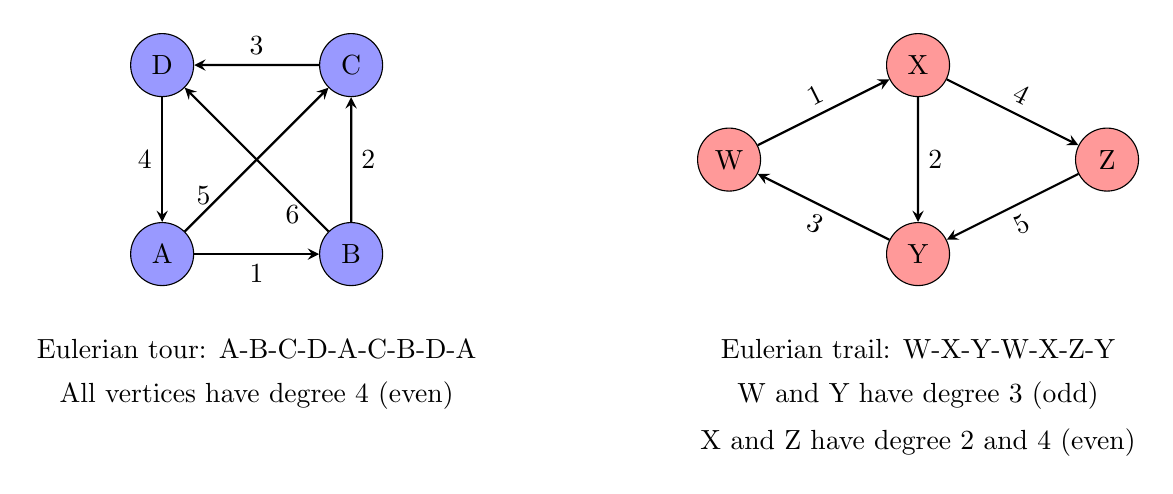
\begin{tikzpicture}[scale=1.2]
    % Example 3: Graph with Eulerian tour - showing the tour
    \begin{scope}[shift={(-2.5,0)}]
        % Vertices
        \node[circle, draw, fill=blue!40, minimum size=0.8cm] (A) at (0,0) {A};
        \node[circle, draw, fill=blue!40, minimum size=0.8cm] (B) at (2,0) {B};
        \node[circle, draw, fill=blue!40, minimum size=0.8cm] (C) at (2,2) {C};
        \node[circle, draw, fill=blue!40, minimum size=0.8cm] (D) at (0,2) {D};
        
        % Edges with directed arrows showing an Eulerian tour
        \draw[thick, ->, >=stealth] (A) -- node[below] {1} (B);
        \draw[thick, ->, >=stealth] (B) -- node[right] {2} (C);
        \draw[thick, ->, >=stealth] (C) -- node[above] {3} (D);
        \draw[thick, ->, >=stealth] (D) -- node[left] {4} (A);
        \draw[thick, ->, >=stealth] (A) -- node[near start, left] {5} (C);
        \draw[thick, ->, >=stealth] (B) -- node[near start, below] {6} (D);
        
        \node at (1,-1) {Eulerian tour: A-B-C-D-A-C-B-D-A};
        \node at (1,-1.5) {All vertices have degree 4 (even)};
    \end{scope}
    
    % Example 4: Graph with Eulerian trail but no tour - showing the trail
    \begin{scope}[shift={(3.5,0)}]
        % Vertices
        \node[circle, draw, fill=red!40, minimum size=0.8cm] (W) at (0,1) {W};
        \node[circle, draw, fill=red!40, minimum size=0.8cm] (X) at (2,2) {X};
        \node[circle, draw, fill=red!40, minimum size=0.8cm] (Y) at (2,0) {Y};
        \node[circle, draw, fill=red!40, minimum size=0.8cm] (Z) at (4,1) {Z};
        
        % Edges with directed arrows showing an Eulerian trail
        \draw[thick, ->, >=stealth] (W) -- node[above, sloped] {1} (X);
        \draw[thick, ->, >=stealth] (X) -- node[right] {2} (Y);
        \draw[thick, ->, >=stealth] (Y) -- node[below, sloped] {3} (W);
        \draw[thick, ->, >=stealth] (X) -- node[above, sloped] {4} (Z);
        \draw[thick, ->, >=stealth] (Z) -- node[below, sloped] {5} (Y);
        
        \node at (2,-1) {Eulerian trail: W-X-Y-W-X-Z-Y};
        \node at (2,-1.5) {W and Y have degree 3 (odd)};
        \node at (2,-2) {X and Z have degree 2 and 4 (even)};
    \end{scope}
\end{tikzpicture}

\vspace{0.3cm}
{\centering
\small Figure 27: Explicit examples of Eulerian tours and trails. Left: A graph where every vertex has even degree (4), with a complete Eulerian tour shown by numbered edges. The tour visits every edge exactly once and returns to the starting vertex A. Right: A graph with exactly two odd-degree vertices (W and Y), showing an Eulerian trail that traverses every edge exactly once but doesn't form a closed circuit.
\par}
\end{figure}

\begin{proof}[Proof of (1)]
$(\Rightarrow)$ Suppose there is an Eulerian tour $C = v_1, v_2, \ldots, v_m, v_1$. We prove all vertices have even degree by induction on $|E(G)|$.

Base case: $|E(G)| = 1$. The Eulerian tour is $v_1, v_1$, so $d(v_1) = 2$.

Suppose the strong induction statement is true for all graphs with fewer than $m$ edges.
Let $C = v_1, v_2, \ldots, v_m, v_1$ be an Eulerian tour in $G$ with $m$ edges.
Let $j = \min\{i > 1 : v_i = v_j \text{ for some } j < i\}$.

If $j = m+1$, then the entire tour is a simple cycle with $m$ edges, so every vertex has degree 2.

If $j < m+1$:
\begin{itemize}
\item Remove all edges $\{v_1, v_2\}, \{v_2, v_3\}, \ldots, \{v_{j-1}, v_j\}$
\end{itemize}

By induction, the remaining edges form an Eulerian tour $v_j, v_{j+1}, \ldots, v_m, v_1$, so all vertices in this subgraph have even degree.
Also, $C' = v_1, v_2, \ldots, v_j$ is also an Eulerian tour in its subgraph, so all those vertices have even degree.
Therefore, all vertices in the original graph have even degree.

$(\Leftarrow)$ Let $C = v_1, v_2, \ldots, v_n$ be a longest trail in the graph.

Case 1: Suppose $v_n \neq v_1$.
Since $v_n$ has even degree, we know an edge $\{v_n, v_{n+1}\}$ not in the trail exists.
Now $C' = v_1, v_2, \ldots, v_n, v_{n+1}$ is a longer trail, a contradiction.

Case 2: $v_n = v_1$.
Since $G$ is connected, all edges must be used by the trail.
Otherwise, relabel the trail as $v'_1, v'_2, \ldots, v'_{n-1}, v'_n = v'_1$.
We can add $\{v'_i, v'_{n+1}\}$ to create a longer trail, contradiction.
Therefore, the graph has an Eulerian tour.
\end{proof}

\begin{figure}[ht]
\centering
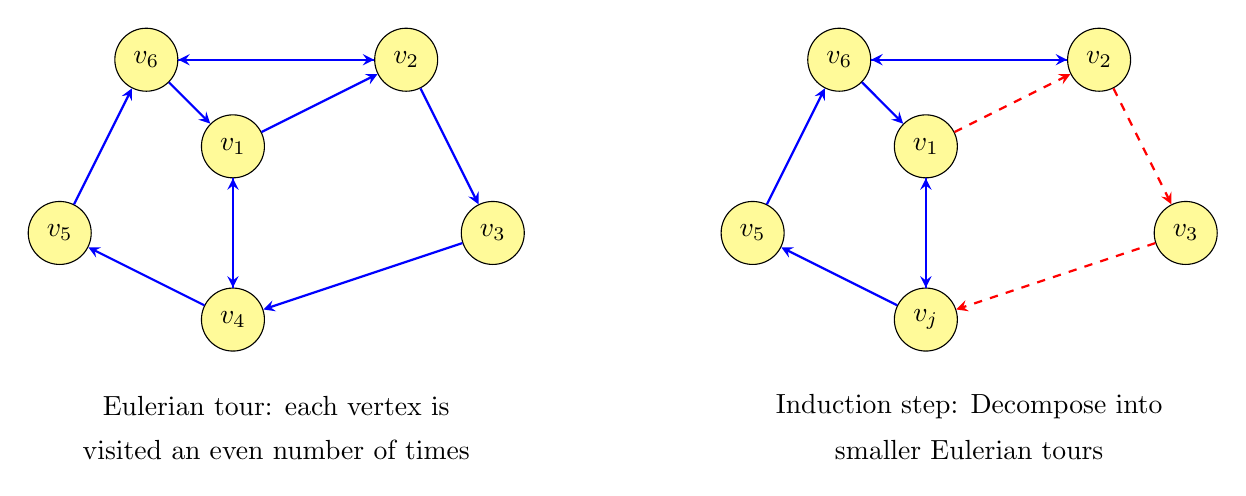
\begin{tikzpicture}[scale=1.1]
    % Visual for the forward direction of the proof
    \begin{scope}[shift={(-4,0)}]
        % Original graph
        \node[circle, draw, fill=yellow!40, minimum size=0.8cm] (A) at (0,0) {$v_1$};
        \node[circle, draw, fill=yellow!40, minimum size=0.8cm] (B) at (2,1) {$v_2$};
        \node[circle, draw, fill=yellow!40, minimum size=0.8cm] (C) at (3,-1) {$v_3$};
        \node[circle, draw, fill=yellow!40, minimum size=0.8cm] (D) at (0,-2) {$v_4$};
        \node[circle, draw, fill=yellow!40, minimum size=0.8cm] (E) at (-2,-1) {$v_5$};
        \node[circle, draw, fill=yellow!40, minimum size=0.8cm] (F) at (-1,1) {$v_6$};
        
        % Eulerian tour - directed arrows
        \draw[thick, ->, >=stealth, blue] (A) -- (B);
        \draw[thick, ->, >=stealth, blue] (B) -- (C);
        \draw[thick, ->, >=stealth, blue] (C) -- (D);
        \draw[thick, ->, >=stealth, blue] (D) -- (E);
        \draw[thick, ->, >=stealth, blue] (E) -- (F);
        \draw[thick, ->, >=stealth, blue] (F) -- (A);
        \draw[thick, ->, >=stealth, blue] (A) -- (D);
        \draw[thick, ->, >=stealth, blue] (D) -- (A);
        \draw[thick, ->, >=stealth, blue] (B) -- (F);
        \draw[thick, ->, >=stealth, blue] (F) -- (B);

        \node at (0.5,-3) {Eulerian tour: each vertex is};
        \node at (0.5,-3.5) {visited an even number of times};
    \end{scope}
    
    % Visual for the induction step - decomposition
    \begin{scope}[shift={(4,0)}]
        % Original graph structure
        \node[circle, draw, fill=yellow!40, minimum size=0.8cm] (A) at (0,0) {$v_1$};
        \node[circle, draw, fill=yellow!40, minimum size=0.8cm] (B) at (2,1) {$v_2$};
        \node[circle, draw, fill=yellow!40, minimum size=0.8cm] (C) at (3,-1) {$v_3$};
        \node[circle, draw, fill=yellow!40, minimum size=0.8cm] (D) at (0,-2) {$v_j$};
        \node[circle, draw, fill=yellow!40, minimum size=0.8cm] (E) at (-2,-1) {$v_5$};
        \node[circle, draw, fill=yellow!40, minimum size=0.8cm] (F) at (-1,1) {$v_6$};
        
        % First cycle (removed in induction)
        \draw[thick, ->, >=stealth, red, dashed] (A) -- (B);
        \draw[thick, ->, >=stealth, red, dashed] (B) -- (C);
        \draw[thick, ->, >=stealth, red, dashed] (C) -- (D);
        
        % Second cycle (remaining after removal)
        \draw[thick, ->, >=stealth, blue] (D) -- (E);
        \draw[thick, ->, >=stealth, blue] (E) -- (F);
        \draw[thick, ->, >=stealth, blue] (F) -- (A);
        \draw[thick, ->, >=stealth, blue] (A) -- (D);
        \draw[thick, ->, >=stealth, blue] (D) -- (A);
        \draw[thick, ->, >=stealth, blue] (B) -- (F);
        \draw[thick, ->, >=stealth, blue] (F) -- (B);
        
        \node at (0.5,-3) {Induction step: Decompose into};
        \node at (0.5,-3.5) {smaller Eulerian tours};
    \end{scope}
\end{tikzpicture}

\vspace{0.3cm}
{\centering
\small Figure 28: Visualization of the forward direction proof - showing why Eulerian tours imply even degrees. Left: A graph with an Eulerian tour (blue arrows) where each vertex must be visited and departed from an equal number of times, giving each vertex an even degree. Right: The induction step showing how an Eulerian tour can be decomposed into smaller Eulerian subcircuits.
\par}
\end{figure}

\begin{figure}[ht]
\centering
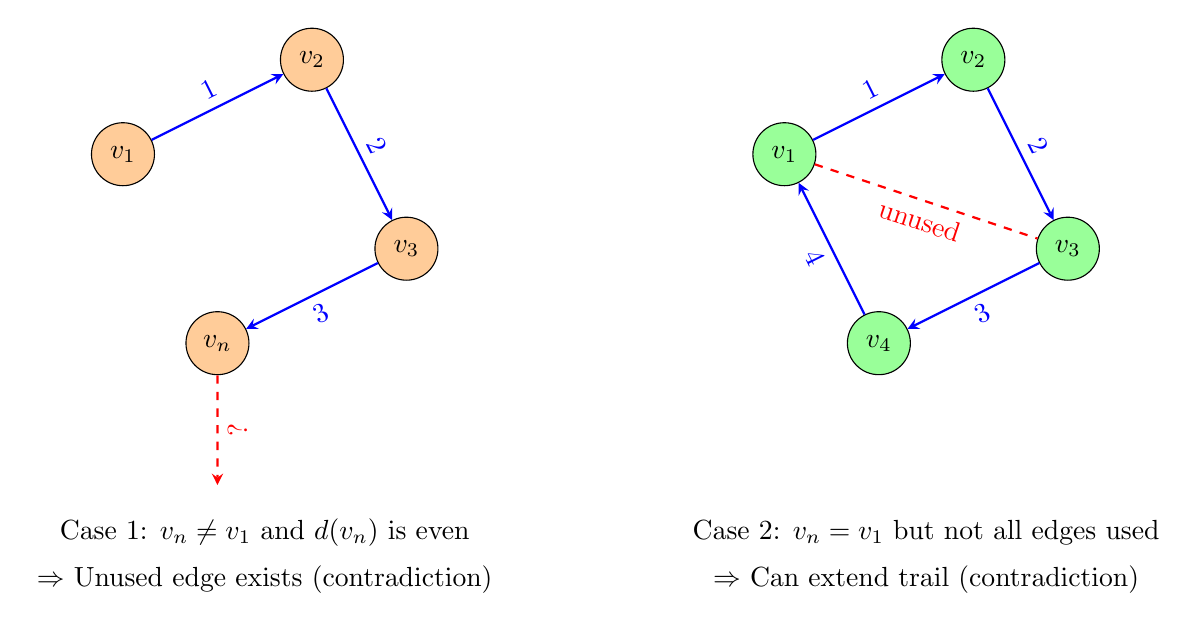
\begin{tikzpicture}[scale=1.2]
    % Case 1 visualization - trail does not end at starting vertex
    \begin{scope}[shift={(-3.5,0)}]
        % Vertices
        \node[circle, draw, fill=orange!40, minimum size=0.8cm] (A) at (0,0) {$v_1$};
        \node[circle, draw, fill=orange!40, minimum size=0.8cm] (B) at (2,1) {$v_2$};
        \node[circle, draw, fill=orange!40, minimum size=0.8cm] (C) at (3,-1) {$v_3$};
        \node[circle, draw, fill=orange!40, minimum size=0.8cm] (D) at (1,-2) {$v_n$};
        
        % Existing trail
        \draw[thick, ->, >=stealth, blue] (A) -- node[above, sloped] {1} (B);
        \draw[thick, ->, >=stealth, blue] (B) -- node[above, sloped] {2} (C);
        \draw[thick, ->, >=stealth, blue] (C) -- node[below, sloped] {3} (D);
        
        % Unused edge from v_n (must exist if degree is even)
        \draw[thick, ->, >=stealth, red, dashed] (D) -- node[below, sloped] {?} (1,-3.5);
        
        \node at (1.5,-4) {Case 1: $v_n \neq v_1$ and $d(v_n)$ is even};
        \node at (1.5,-4.5) {$\Rightarrow$ Unused edge exists (contradiction)};
    \end{scope}
    
    % Case 2 visualization - tour that doesn't use all edges
    \begin{scope}[shift={(3.5,0)}]
        % Vertices
        \node[circle, draw, fill=green!40, minimum size=0.8cm] (A) at (0,0) {$v_1$};
        \node[circle, draw, fill=green!40, minimum size=0.8cm] (B) at (2,1) {$v_2$};
        \node[circle, draw, fill=green!40, minimum size=0.8cm] (C) at (3,-1) {$v_3$};
        \node[circle, draw, fill=green!40, minimum size=0.8cm] (D) at (1,-2) {$v_4$};
        
        % Existing tour edges
        \draw[thick, ->, >=stealth, blue] (A) -- node[above, sloped] {1} (B);
        \draw[thick, ->, >=stealth, blue] (B) -- node[above, sloped] {2} (C);
        \draw[thick, ->, >=stealth, blue] (C) -- node[below, sloped] {3} (D);
        \draw[thick, ->, >=stealth, blue] (D) -- node[below, sloped] {4} (A);
        
        % Unused edge (contradiction in connected graph)
        \draw[thick, red, dashed] (A) -- node[below, sloped] {unused} (C);
        
        \node at (1.5,-4) {Case 2: $v_n = v_1$ but not all edges used};
        \node at (1.5,-4.5) {$\Rightarrow$ Can extend trail (contradiction)};
    \end{scope}
\end{tikzpicture}

\vspace{0.3cm}
{\centering
\small Figure 29: Visualization of the reverse direction proof - showing why even degrees imply Eulerian tours. Left: If the longest trail doesn't end at its starting point and the final vertex has even degree, an unused edge must exist (contradiction). Right: If the trail forms a tour but doesn't use all edges, the graph has another edge that could extend the tour (contradiction).
\par}
\end{figure}

\begin{proof}[Proof of (2)]
$(\Rightarrow)$ Suppose $G$ has an Eulerian trail from $u$ to $v$ with $u \neq v$. Add an edge $e$ between $u$ and $v$. The resulting graph $G' = G \cup \{e\}$ has an Eulerian tour. By part (1), all vertices in $G'$ have even degree.

In the original graph $G$, the degrees of $u$ and $v$ are both reduced by 1, making them odd, while all other vertices maintain their even degree.

$(\Leftarrow)$ Suppose $u$ and $v$ have odd degree, and all other vertices have even degree. Add an edge $e$ between $u$ and $v$. In the resulting graph $G' = G \cup \{e\}$, all vertices now have even degree.

By part (1), $G'$ has an Eulerian tour. This tour must use the edge $e$ at some point. Remove $e$ from the tour, and we obtain an Eulerian trail in $G$ from $u$ to $v$.
\end{proof}

\begin{figure}[ht]
\centering
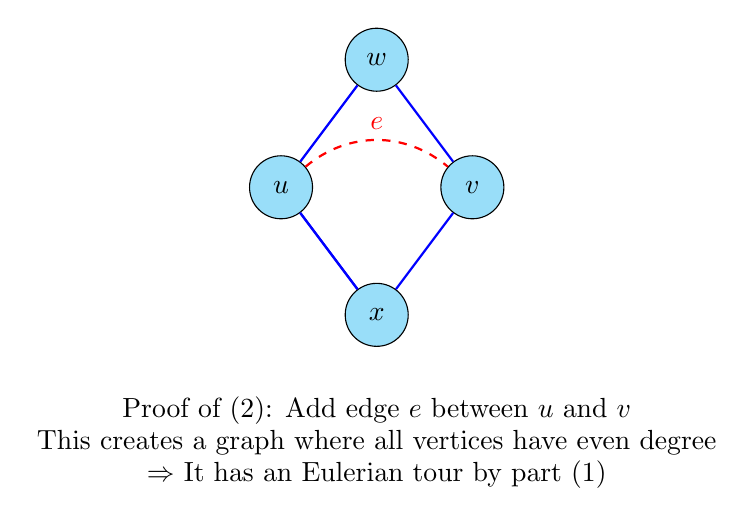
\begin{tikzpicture}[scale=0.81]
    % Graph with Eulerian trail
    \begin{scope}[shift={(0,0)}]
        % Vertices
        \node[circle, draw, fill=cyan!40, minimum size=0.8cm] (A) at (0,0) {$u$};
        \node[circle, draw, fill=cyan!40, minimum size=0.8cm] (B) at (3,0) {$v$};
        \node[circle, draw, fill=cyan!40, minimum size=0.8cm] (C) at (1.5,2) {$w$};
        \node[circle, draw, fill=cyan!40, minimum size=0.8cm] (D) at (1.5,-2) {$x$};
        
        % Original graph edges - Eulerian trail
        \draw[thick, blue] (A) -- (C);
        \draw[thick, blue] (C) -- (B);
        \draw[thick, blue] (B) -- (D);
        \draw[thick, blue] (D) -- (A);
        \draw[thick, blue] (A) -- (D);
        
        % Additional edge to create Eulerian tour
        \draw[thick, red, dashed] (A) to[bend left=40] node[above] {$e$} (B);
        
        \node at (1.5,-3.5) {Proof of (2): Add edge $e$ between $u$ and $v$};
        \node at (1.5,-4) {This creates a graph where all vertices have even degree};
        \node at (1.5,-4.5) {$\Rightarrow$ It has an Eulerian tour by part (1)};
    \end{scope}
\end{tikzpicture}

\vspace{0.3cm}
{\centering
\small Figure 30: Visualization of the proof for part (2) - Converting between Eulerian trails and tours. By adding a new edge $e$ (red dashed line) between the two odd-degree vertices $u$ and $v$, we transform the graph into one where every vertex has even degree. This creates a graph with an Eulerian tour, and removing edge $e$ gives us the original Eulerian trail.
\par}
\end{figure}

% Fleury's Algorithm - Figure Descriptions in LaTeX

\setcounter{figure}{30} % This sets the figure counter to 30, so the next figure will be 31

\begin{figure}[p]
{\centering
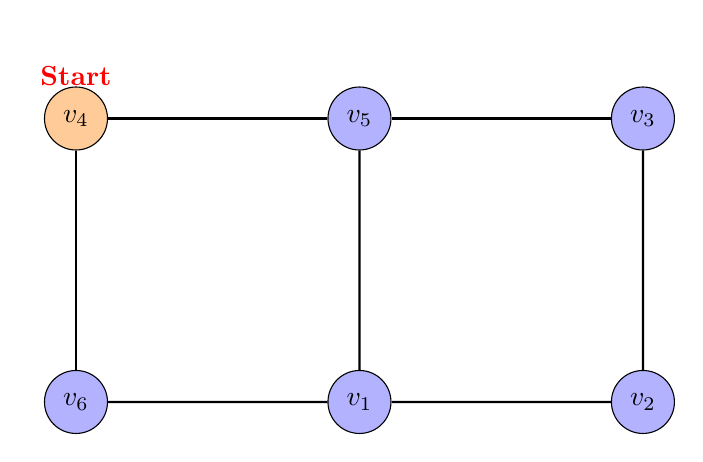
\begin{tikzpicture}[scale=1.8, 
    every node/.style={circle, draw, minimum size=0.8cm}]
    % Vertices
    \node[fill=orange!40] (v4) at (0,0) {$v_4$};
    \node[fill=blue!30] (v5) at (2,0) {$v_5$};
    \node[fill=blue!30] (v3) at (4,0) {$v_3$};
    \node[fill=blue!30] (v6) at (0,-2) {$v_6$};
    \node[fill=blue!30] (v1) at (2,-2) {$v_1$};
    \node[fill=blue!30] (v2) at (4,-2) {$v_2$};
    
    % Edges
    \draw[thick] (v4) -- (v5);
    \draw[thick] (v5) -- (v3);
    \draw[thick] (v4) -- (v6);
    \draw[thick] (v6) -- (v1);
    \draw[thick] (v1) -- (v2);
    \draw[thick] (v2) -- (v3);
    \draw[thick] (v1) -- (v5);
    
    % Start marker
    \node[text=red, font=\bfseries, draw=none, fill=none, minimum size=0cm] at (0,0.3) {Start};
\end{tikzpicture}
\par}
{\centering
\small Figure 31: Graph for applying Fleury's Algorithm. This figure displays the initial connected graph with six vertices labeled $v_1$ through $v_6$ arranged in a rectangular pattern. Vertex $v_4$ is highlighted in orange as the starting point, indicated by the red ``Start'' label. The graph has seven edges connecting the vertices in a way that allows for an Eulerian trail.
\par}
\end{figure}

\begin{figure}[p]
{\centering
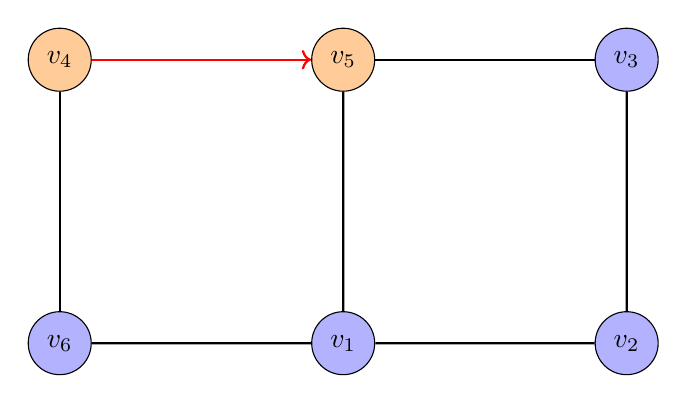
\begin{tikzpicture}[scale=1.8, 
    every node/.style={circle, draw, minimum size=0.8cm}]
    % Vertices - Step 1
    \node[fill=orange!40] (v4) at (0,0) {$v_4$};
    \node[fill=orange!40] (v5) at (2,0) {$v_5$};
    \node[fill=blue!30] (v3) at (4,0) {$v_3$};
    \node[fill=blue!30] (v6) at (0,-2) {$v_6$};
    \node[fill=blue!30] (v1) at (2,-2) {$v_1$};
    \node[fill=blue!30] (v2) at (4,-2) {$v_2$};
    
    % Edges
    \draw[thick, red, ->] (v4) -- (v5);
    \draw[thick] (v5) -- (v3);
    \draw[thick] (v4) -- (v6);
    \draw[thick] (v6) -- (v1);
    \draw[thick] (v1) -- (v2);
    \draw[thick] (v2) -- (v3);
    \draw[thick] (v1) -- (v5);
\end{tikzpicture}
\par}
{\centering
\small Figure 32: Step 1: Choose edge $\{v_4,v_5\}$. This figure shows the first step of Fleury's Algorithm. Vertices $v_4$ and $v_5$ are both highlighted in orange, with a red directed arrow indicating the traversal from $v_4$ to $v_5$. This represents the first edge chosen in the Eulerian trail.
\par}
\end{figure}

\begin{figure}[p]
{\centering
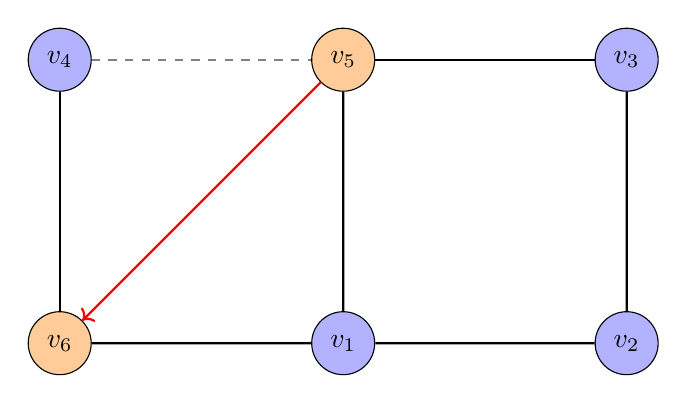
\begin{tikzpicture}[scale=1.8, 
    every node/.style={circle, draw, minimum size=0.8cm}]
    % Vertices - Step 2
    \node[fill=blue!30] (v4) at (0,0) {$v_4$};
    \node[fill=orange!40] (v5) at (2,0) {$v_5$};
    \node[fill=blue!30] (v3) at (4,0) {$v_3$};
    \node[fill=orange!40] (v6) at (0,-2) {$v_6$};
    \node[fill=blue!30] (v1) at (2,-2) {$v_1$};
    \node[fill=blue!30] (v2) at (4,-2) {$v_2$};
    
    % Edges
    \draw[thick, dashed, gray] (v4) -- (v5);
    \draw[thick] (v5) -- (v3);
    \draw[thick] (v4) -- (v6);
    \draw[thick] (v6) -- (v1);
    \draw[thick] (v1) -- (v2);
    \draw[thick] (v2) -- (v3);
    \draw[thick, red, ->] (v5) -- (v6);
    \draw[thick] (v1) -- (v5);
\end{tikzpicture}
\par}
{\centering
\small Figure 33: Step 2: Choose edge $\{v_5,v_6\}$. Vertices $v_5$ and $v_6$ are highlighted in orange. The previously traversed edge (from $v_4$ to $v_5$) is shown as a dashed gray line. A red directed arrow connects $v_5$ to $v_6$, showing the second edge chosen in the algorithm, following the rule of selecting edges that don't disconnect the graph.
\par}
\end{figure}

\begin{figure}[p]
{\centering
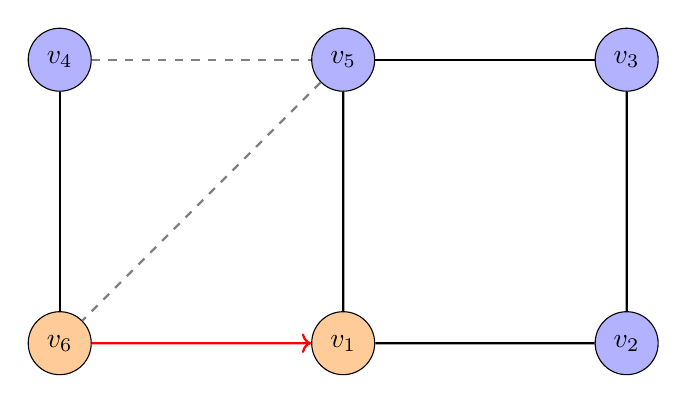
\begin{tikzpicture}[scale=1.8, 
    every node/.style={circle, draw, minimum size=0.8cm}]
    % Vertices - Step 3
    \node[fill=blue!30] (v4) at (0,0) {$v_4$};
    \node[fill=blue!30] (v5) at (2,0) {$v_5$};
    \node[fill=blue!30] (v3) at (4,0) {$v_3$};
    \node[fill=orange!40] (v6) at (0,-2) {$v_6$};
    \node[fill=orange!40] (v1) at (2,-2) {$v_1$};
    \node[fill=blue!30] (v2) at (4,-2) {$v_2$};
    
    % Edges
    \draw[thick, dashed, gray] (v4) -- (v5);
    \draw[thick] (v5) -- (v3);
    \draw[thick] (v4) -- (v6);
    \draw[thick, red, ->] (v6) -- (v1);
    \draw[thick] (v1) -- (v2);
    \draw[thick] (v2) -- (v3);
    \draw[thick, dashed, gray] (v5) -- (v6);
    \draw[thick] (v1) -- (v5);
\end{tikzpicture}
\par}
{\centering
\small Figure 34: Step 3: Choose edge $\{v_6,v_1\}$. Vertices $v_6$ and $v_1$ are highlighted in orange. Previously traversed edges ($v_4$-$v_5$ and $v_5$-$v_6$) are shown as dashed gray lines. A red directed arrow connects $v_6$ to $v_1$, representing the current edge being traversed in the Eulerian trail.
\par}
\end{figure}

\begin{figure}[p]
{\centering
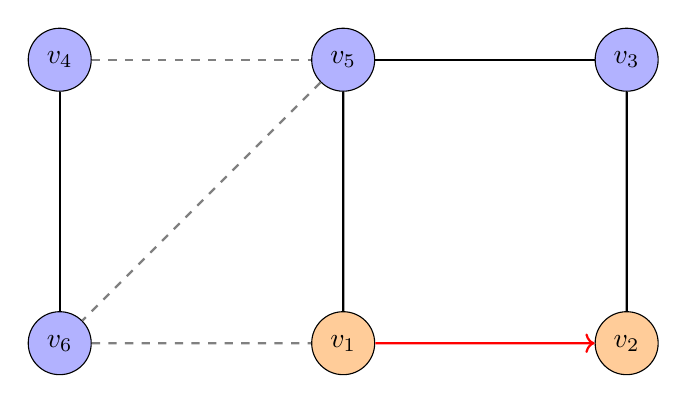
\begin{tikzpicture}[scale=1.8, 
    every node/.style={circle, draw, minimum size=0.8cm}]
    % Vertices - Step 4
    \node[fill=blue!30] (v4) at (0,0) {$v_4$};
    \node[fill=blue!30] (v5) at (2,0) {$v_5$};
    \node[fill=blue!30] (v3) at (4,0) {$v_3$};
    \node[fill=blue!30] (v6) at (0,-2) {$v_6$};
    \node[fill=orange!40] (v1) at (2,-2) {$v_1$};
    \node[fill=orange!40] (v2) at (4,-2) {$v_2$};
    
    % Edges
    \draw[thick, dashed, gray] (v4) -- (v5);
    \draw[thick] (v5) -- (v3);
    \draw[thick] (v4) -- (v6);
    \draw[thick, dashed, gray] (v6) -- (v1);
    \draw[thick, red, ->] (v1) -- (v2);
    \draw[thick] (v2) -- (v3);
    \draw[thick, dashed, gray] (v5) -- (v6);
    \draw[thick] (v1) -- (v5);
\end{tikzpicture}
\par}
{\centering
\small Figure 35: Step 4: Choose edge $\{v_1,v_2\}$. Vertices $v_1$ and $v_2$ are highlighted in orange. Three edges have now been traversed and appear as dashed gray lines. The current traversal from $v_1$ to $v_2$ is shown with a red directed arrow, continuing to follow the principle of choosing edges that maintain connectivity when possible.
\par}
\end{figure}

\begin{figure}[p]
{\centering
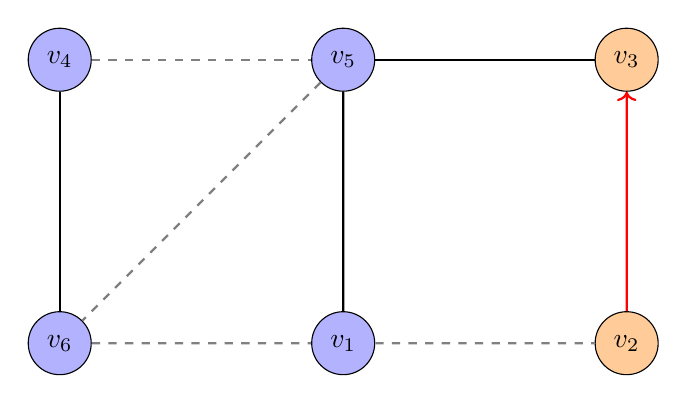
\begin{tikzpicture}[scale=1.8, 
    every node/.style={circle, draw, minimum size=0.8cm}]
    % Vertices - Step 5
    \node[fill=blue!30] (v4) at (0,0) {$v_4$};
    \node[fill=blue!30] (v5) at (2,0) {$v_5$};
    \node[fill=orange!40] (v3) at (4,0) {$v_3$};
    \node[fill=blue!30] (v6) at (0,-2) {$v_6$};
    \node[fill=blue!30] (v1) at (2,-2) {$v_1$};
    \node[fill=orange!40] (v2) at (4,-2) {$v_2$};
    
    % Edges
    \draw[thick, dashed, gray] (v4) -- (v5);
    \draw[thick] (v5) -- (v3);
    \draw[thick] (v4) -- (v6);
    \draw[thick, dashed, gray] (v6) -- (v1);
    \draw[thick, dashed, gray] (v1) -- (v2);
    \draw[thick, red, ->] (v2) -- (v3);
    \draw[thick, dashed, gray] (v5) -- (v6);
    \draw[thick] (v1) -- (v5);
\end{tikzpicture}
\par}
{\centering
\small Figure 36: Step 5: Choose edge $\{v_2,v_3\}$. Vertices $v_2$ and $v_3$ are highlighted in orange. Four previously traversed edges are shown as dashed gray lines. The current edge being traversed from $v_2$ to $v_3$ is indicated by a red directed arrow.
\par}
\end{figure}

\begin{figure}[p]
{\centering
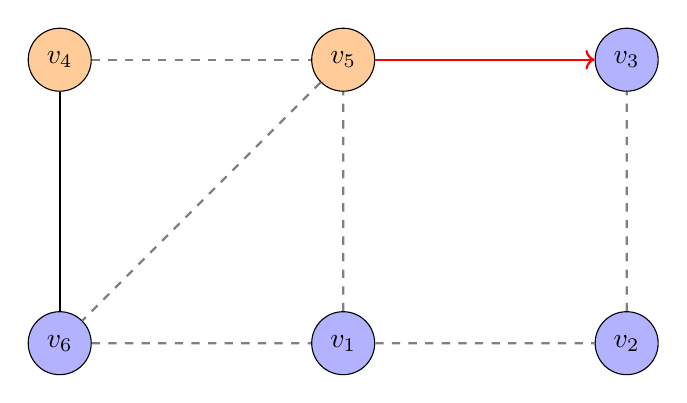
\begin{tikzpicture}[scale=1.8, 
    every node/.style={circle, draw, minimum size=0.8cm}]
    % Vertices - Step 6
    \node[fill=orange!40] (v4) at (0,0) {$v_4$};
    \node[fill=orange!40] (v5) at (2,0) {$v_5$};
    \node[fill=blue!30] (v3) at (4,0) {$v_3$};
    \node[fill=blue!30] (v6) at (0,-2) {$v_6$};
    \node[fill=blue!30] (v1) at (2,-2) {$v_1$};
    \node[fill=blue!30] (v2) at (4,-2) {$v_2$};
    
    % Edges
    \draw[thick, dashed, gray] (v4) -- (v5);
    \draw[thick, red, ->] (v5) -- (v3);
    \draw[thick] (v4) -- (v6);
    \draw[thick, dashed, gray] (v6) -- (v1);
    \draw[thick, dashed, gray] (v1) -- (v2);
    \draw[thick, dashed, gray] (v2) -- (v3);
    \draw[thick, dashed, gray] (v5) -- (v6);
    \draw[thick, dashed, gray] (v1) -- (v5);
\end{tikzpicture}
\par}
{\centering
\small Figure 37: Step 6: Choose edge $\{v_5,v_3\}$. Vertices $v_4$ and $v_5$ are highlighted in orange. Most edges have been traversed (shown as dashed gray lines). The current traversal is from $v_5$ to $v_3$, indicated by a red directed arrow. Note that the algorithm now traverses the remaining edges to complete the Eulerian trail.
\par}
\end{figure}

\begin{figure}[p]
{\centering
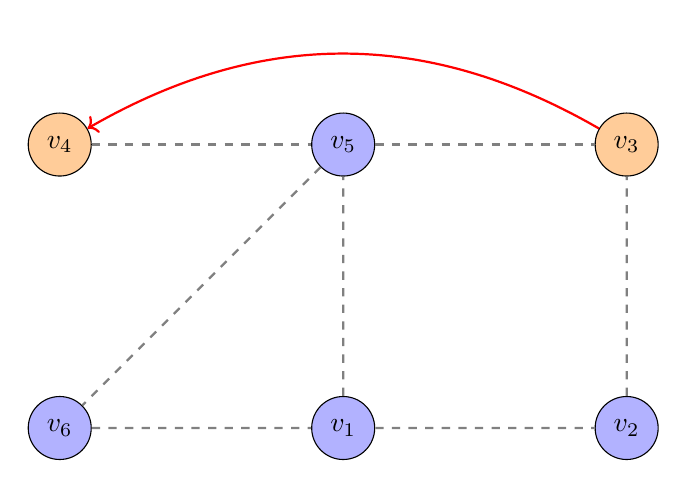
\begin{tikzpicture}[scale=1.8, 
    every node/.style={circle, draw, minimum size=0.8cm}]
    % Vertices - Step 7
    \node[fill=orange!40] (v4) at (0,0) {$v_4$};
    \node[fill=blue!30] (v5) at (2,0) {$v_5$};
    \node[fill=orange!40] (v3) at (4,0) {$v_3$};
    \node[fill=blue!30] (v6) at (0,-2) {$v_6$};
    \node[fill=blue!30] (v1) at (2,-2) {$v_1$};
    \node[fill=blue!30] (v2) at (4,-2) {$v_2$};
    
    % Edges
    \draw[thick, dashed, gray] (v4) -- (v5);
    \draw[thick, dashed, gray] (v5) -- (v3);
    \draw[thick, red, ->] (v3) to[bend right=30] (v4);
    \draw[thick, dashed, gray] (v6) -- (v1);
    \draw[thick, dashed, gray] (v1) -- (v2);
    \draw[thick, dashed, gray] (v2) -- (v3);
    \draw[thick, dashed, gray] (v5) -- (v6);
    \draw[thick, dashed, gray] (v1) -- (v5);
    
\end{tikzpicture}
\par}
{\centering
\small Figure 38: Step 7: Choose final edge $\{v_3,v_4\}$ to complete the tour. Vertices $v_4$ and $v_3$ are highlighted in orange with a red directed arrow from $v_3$ to $v_4$. This represents the completion of the Eulerian trail as the algorithm returns to the starting vertex after having traversed all edges in the graph exactly once.
\par}
\end{figure}

\begin{figure}[p]
{\centering
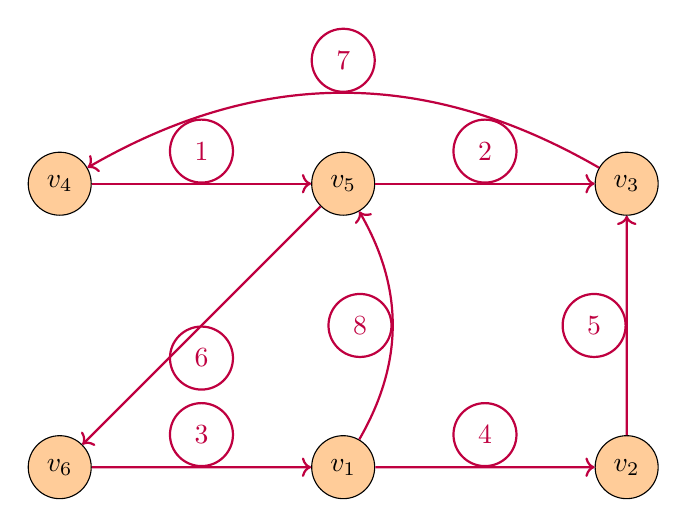
\begin{tikzpicture}[scale=1.8, 
    every node/.style={circle, draw, minimum size=0.8cm}]
    
    % Full tour
    \node[fill=orange!40] (v4) at (0,0) {$v_4$};
    \node[fill=orange!40] (v5) at (2,0) {$v_5$};
    \node[fill=orange!40] (v3) at (4,0) {$v_3$};
    \node[fill=orange!40] (v6) at (0,-2) {$v_6$};
    \node[fill=orange!40] (v1) at (2,-2) {$v_1$};
    \node[fill=orange!40] (v2) at (4,-2) {$v_2$};
    
    % Completed tour edges
    \draw[->, thick, purple] (v4) to node[above] {1} (v5);
    \draw[->, thick, purple] (v5) to node[below] {6} (v6);
    \draw[->, thick, purple] (v6) to node[above] {3} (v1);
    \draw[->, thick, purple] (v1) to node[above] {4} (v2);
    \draw[->, thick, purple] (v2) to node[left] {5} (v3);
    \draw[->, thick, purple] (v3) to[bend right=30] node[above] {7} (v4);
    \draw[->, thick, purple] (v5) to node[above] {2} (v3);
    \draw[->, thick, purple] (v1) to[bend right=30] node[left] {8} (v5);
\end{tikzpicture}
\par}
{\centering
\small Figure 39: Complete Eulerian tour using Fleury's Algorithm: $v_4 \rightarrow v_5 \rightarrow v_3 \rightarrow v_4 \rightarrow v_6 \rightarrow v_1 \rightarrow v_2 \rightarrow v_3$. All vertices are highlighted in orange, and all edges are shown as purple directed arrows with numbers indicating the order of traversal (1-8). This figure displays the entire Eulerian path found by the algorithm, showing how every edge in the graph is traversed exactly once.
\par}
\end{figure}

\begin{figure}[p]
{\centering
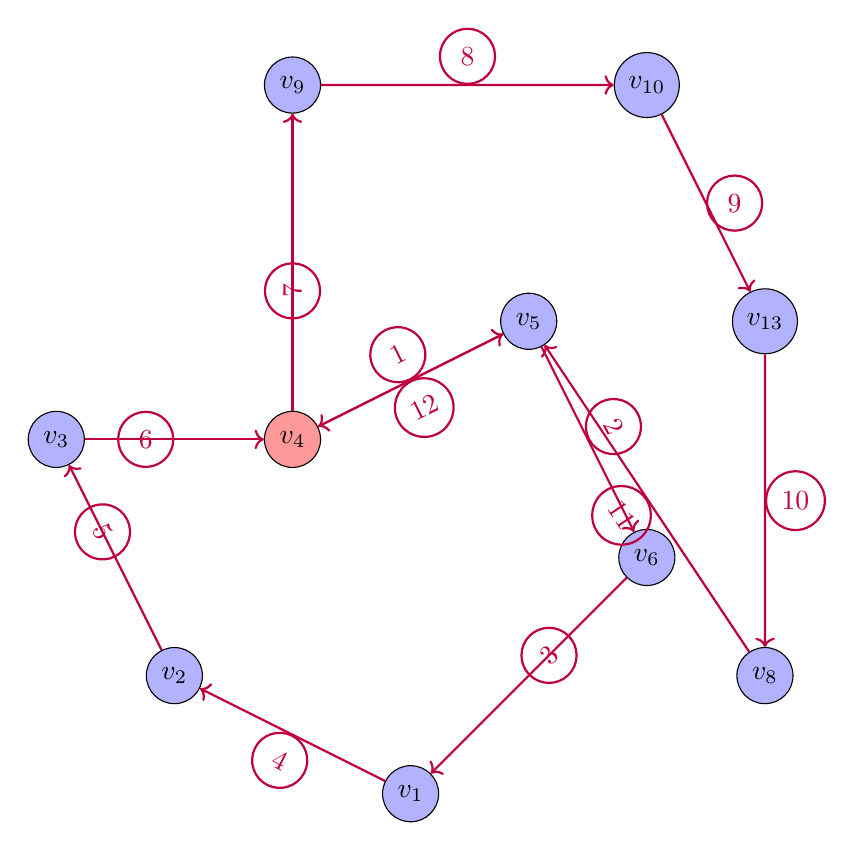
\begin{tikzpicture}[scale=1.5,
    every node/.style={circle, draw, minimum size=0.7cm}]
    % Vertices for the example
    \node[fill=red!40] (v4) at (0,0) {$v_4$};
    \node[fill=blue!30] (v5) at (2,1) {$v_5$};
    \node[fill=blue!30] (v6) at (3,-1) {$v_6$};
    \node[fill=blue!30] (v1) at (1,-3) {$v_1$};
    \node[fill=blue!30] (v2) at (-1,-2) {$v_2$};
    \node[fill=blue!30] (v3) at (-2,0) {$v_3$};
    \node[fill=blue!30] (v9) at (0,3) {$v_9$};
    \node[fill=blue!30] (v10) at (3,3) {$v_{10}$};
    \node[fill=blue!30] (v13) at (4,1) {$v_{13}$};
    \node[fill=blue!30] (v8) at (4,-2) {$v_8$};
    
    % Edges for the example
    \draw[->, thick, purple] (v4) to node[above, sloped] {1} (v5);
    \draw[->, thick, purple] (v5) to node[above, sloped] {2} (v6);
    \draw[->, thick, purple] (v6) to node[right, sloped] {3} (v1);
    \draw[->, thick, purple] (v1) to node[below, sloped] {4} (v2);
    \draw[->, thick, purple] (v2) to node[left, sloped] {5} (v3);
    \draw[->, thick, purple] (v3) to node[left, sloped] {6} (v4);
    \draw[->, thick, purple] (v4) to node[left, sloped] {7} (v9);
    \draw[->, thick, purple] (v9) to node[above] {8} (v10);
    \draw[->, thick, purple] (v10) to node[right] {9} (v13);
    \draw[->, thick, purple] (v13) to node[right] {10} (v8);
    \draw[->, thick, purple] (v8) to node[below, sloped] {11} (v5);
    \draw[->, thick, purple] (v5) to node[below, sloped] {12} (v4);
\end{tikzpicture}
\par}
{\centering
\small Figure 40: Example Eulerian tour: $v_4 \rightarrow v_5 \rightarrow v_6 \rightarrow v_1 \rightarrow v_2 \rightarrow v_3 \rightarrow v_4 \rightarrow v_9 \rightarrow v_{10} \rightarrow v_{13} \rightarrow v_8 \rightarrow v_5 \rightarrow v_4$. This figure shows a more complex example of an Eulerian tour on a larger graph with 10 vertices. The starting vertex $v_4$ is highlighted in red, and the complete tour is shown with purple directed arrows numbered 1-12. This demonstrates how Fleury's Algorithm scales to larger graphs while still finding a valid Eulerian path that traverses each edge exactly once before returning to the starting vertex.
\par}

\vspace{1em}
\begin{minipage}{\linewidth}
\begin{algorithm}[H]
\caption{Fleury's Algorithm for finding an Eulerian path or circuit}
\begin{algorithmic}[1]
\Procedure{Fleury}{$G(V,E)$, $start$}
    \State Let $currentVertex \gets start$
    \State Initialize empty list $path$
    \While{$E$ is not empty}
        \If{degree of $currentVertex$ is 1}
            \State Let $nextEdge$ be the only edge incident to $currentVertex$
        \Else
            \State Let $nextEdge$ be any edge incident to $currentVertex$ such that removing $nextEdge$ doesn't disconnect the graph
        \EndIf
        \State Let $nextVertex$ be the vertex at the other end of $nextEdge$
        \State Add $currentVertex$ to $path$
        \State Remove $nextEdge$ from $E$
        \State $currentVertex \gets nextVertex$
    \EndWhile
    \State Add $currentVertex$ to $path$ \Comment{Add the final vertex}
    \State \Return $path$
\EndProcedure
\end{algorithmic}
\end{algorithm}
\end{minipage}
\end{figure}

\pagebreak

\subsection{Eulerian Digraphs and DeBruijn Sequences}
\subsubsection{Eulerian Digraphs}

\begin{definition}[Eulerian Directed Graphs]
A directed graph (digraph) is Eulerian if there exists a closed walk that traverses each edge exactly once. The following properties characterize Eulerian digraphs:
\begin{enumerate}
    \item A digraph is Eulerian if and only if it is connected and the in-degree equals the out-degree for every vertex.
    \item A digraph has an Eulerian path (but not necessarily a cycle) if and only if:
    \begin{itemize}
        \item At most one vertex has $(\text{out-degree}) - (\text{in-degree}) = 1$
        \item At most one vertex has $(\text{in-degree}) - (\text{out-degree}) = 1$
        \item For all other vertices, in-degree equals out-degree
    \end{itemize}
\end{enumerate}
For a directed graph $G = (V, E)$, define:
\begin{align}
    d^+(v) &= \text{out-degree of vertex } v\\
    d^-(v) &= \text{in-degree of vertex } v
\end{align}
Then $G$ is Eulerian if and only if:
\begin{enumerate}
    \item $G$ is connected (or more precisely, the underlying undirected graph of $G$ is connected)
    \item $\forall v \in V, d^+(v) = d^-(v)$
\end{enumerate}
\end{definition}

\subsubsection{De Bruijn Sequences}


\begin{definition}[De Bruijn Sequence]
A De Bruijn sequence $B(k, n)$ is a cyclic sequence of length $k^n$ over an alphabet $A$ of size $k$ such that each possible string of length $n$ appears exactly once as a contiguous substring.
\end{definition}

\begin{properties}[De Bruijn Sequences]
\end{properties}
\vspace{0.5em} % Adds vertical space after the title

\begin{enumerate}
    \item The length of a De Bruijn sequence $B(k, n)$ is $k^n$.
    
    \item Every string of length $n$ over the alphabet appears exactly once as a substring.
    
    \item A De Bruijn sequence $B(k, n)$ can be viewed as a Hamiltonian path in the De Bruijn graph $G(k, n-1)$.
    
    \item The number of distinct De Bruijn sequences $B(k, n)$ is given by:
    \begin{equation}
        \frac{(k!)^{k^{n-1}}}{k^n}
    \end{equation}
    
    \item More specifically, the number of binary De Bruijn sequences $B(2, n)$ is:
    \begin{equation}
        2^{2^{n-1}-n}
    \end{equation}
\end{enumerate}

\begin{properties}[Connection to Eulerian Digraphs]
De Bruijn sequences have a fundamental connection to Eulerian digraphs:
\begin{enumerate}
    \item A De Bruijn graph $G(k, n-1)$ is a directed graph with $k^{n-1}$ vertices, each labeled with a string of length $n-1$.
    \item There is an edge from vertex $u$ to vertex $v$ if the last $n-2$ symbols of $u$ match the first $n-2$ symbols of $v$.
    \item For every vertex in $G(k, n-1)$, the in-degree equals the out-degree (both equal to $k$).
    \item Therefore, $G(k, n-1)$ is an Eulerian digraph.
    \item A De Bruijn sequence $B(k, n)$ corresponds to an Eulerian circuit in $G(k, n-1)$.
\end{enumerate}
\end{properties}

\begin{properties}[Mathematical Structure]
The adjacency matrix $A$ of the De Bruijn graph $G(k, n)$ has the following properties:
\begin{enumerate}
    \item $A$ is a $k^n \times k^n$ matrix.
    \item $A_{i,j} = 1$ if the last $n-1$ symbols of vertex $i$ match the first $n-1$ symbols of vertex $j$.
    \item $A_{i,j} = 0$ otherwise.
    \item The number of Eulerian circuits (and thus De Bruijn sequences) can be computed using the BEST theorem:
    \begin{equation}
        \text{Number of Eulerian circuits} = t_w \prod_{v \in V} (d^+(v) - 1)!
    \end{equation}
    where $t_w$ is the number of oriented spanning trees(refer to def 33) rooted at vertex $w$.
\end{enumerate}
\end{properties}

\begin{properties}[Combinatorial Aspects] The combinatorial aspects of De Bruijn Sequence B(k,n) has the following properties
\begin{enumerate}
    \item A De Bruijn sequence can be constructed from a Eulerian circuit in the De Bruijn graph $G(k, n-1)$.
    \item Every De Bruijn sequence $B(k, n)$ contains $k^n$ distinct substrings of length $n$.
    \item The De Bruijn sequence has a feedback function $f$ that generates the next bit:
    \begin{equation}
        a_{i+n} = f(a_i, a_{i+1}, \ldots, a_{i+n-1})
    \end{equation}
\end{enumerate}
\end{properties}
\begin{theorem}[Generating Function]
For a binary De Bruijn sequence, the generating function can be expressed as:
\begin{equation}
    G(x) = \sum_{i=0}^{2^n-1} a_i x^i \mod (x^{2^n} - 1)
\end{equation}
where $a_i$ represents the $i$-th element in the sequence.
\end{theorem}

\begin{theorem}[LFSR Representation]
A binary De Bruijn sequence can be generated using a Linear Feedback Shift Register with the characteristic polynomial:
\begin{equation}
    p(x) = x^n + c_{n-1}x^{n-1} + \cdots + c_1x + c_0
\end{equation}
The recurrence relation is:
\begin{equation}
    a_{i+n} = c_0a_i \oplus c_1a_{i+1} \oplus \cdots \oplus c_{n-1}a_{i+n-1}
\end{equation}
where $\oplus$ represents the XOR operation.
\end{theorem}

\begin{theorem}[Counting Formula]
The number of distinct De Bruijn sequences $B(k, n)$ is:
\begin{equation}
    N(k, n) = \frac{k!^{k^{n-1}}}{k^n}
\end{equation}

For the binary case $B(2, n)$, the number of distinct sequences is:
\begin{equation}
    N(2, n) = 2^{2^{n-1}-n}
\end{equation}
\end{theorem}

\begin{example}[Small Values]
The number of distinct De Bruijn sequences for small parameters:
\begin{align}
    N(2, 2) &= 1 \\
    N(2, 3) &= 2 \\
    N(2, 4) &= 16 \\
    N(2, 5) &= 2048 \\
    N(3, 2) &= 2 \\
    N(3, 3) &= 48 \\
    N(4, 2) &= 24
\end{align}
\end{example}
\begin{theorem}[FKM Algorithm]
The FKM (Fredricksen, Kessler, Maiorana) algorithm constructs a binary De Bruijn sequence $B(2, n)$ by generating all necklaces of length $n$, ordering them lexicographically, replacing each with its aperiodic prefixes, and concatenating the last bits of these prefixes in order.
\end{theorem}

\begin{algorithm}
\caption{FKM Algorithm for $B(2, n)$}
\begin{algorithmic}[1]
\Require Integer $n \geq 2$
\Ensure Binary De Bruijn sequence $B(2, n)$
\State $S \gets \text{empty sequence}$
\Function{GenerateNecklaces}{$n$}
    \State $N \gets \emptyset$; $\text{seen} \gets \emptyset$
    \For{all binary strings $b$ of length $n$ in lexicographic order}
        \If{$b \notin \text{seen}$}
            \State $\text{necklace} \gets \text{smallest rotation of } b$
            \State $N \gets N \cup \{\text{necklace}\}$; $\text{seen} \gets \text{seen} \cup \{\text{all rotations of } b\}$
        \EndIf
    \EndFor
    \State \Return $N$
\EndFunction
\Function{GetAperiodicPrefixes}{necklace}
    \State $prefixes \gets \emptyset$; $p \gets \text{period of necklace}$
    \For{$i \gets 1$ to $p$}
        \State $prefixes \gets prefixes \cup \{\text{first } i \text{ bits of necklace}\}$
    \EndFor
    \State \Return $prefixes$
\EndFunction
\State $necklaces \gets \text{Sort}(\text{GenerateNecklaces}(n))$
\For{each $necklace$ in $necklaces$}
    \For{each $prefix$ in $\text{GetAperiodicPrefixes}(necklace)$}
        \State $S \gets S \cdot \text{last bit of } prefix$
    \EndFor
\EndFor
\State \Return $S$
\end{algorithmic}
\end{algorithm}

\begin{remark}
The FKM algorithm can also be implemented using Lyndon words:
\end{remark}

\begin{algorithm}
\caption{Lyndon-based FKM Algorithm}
\begin{algorithmic}[1]
\Require Integer $n \geq 2$
\Ensure Binary De Bruijn sequence $B(2, n)$
\Function{IsLyndonWord}{$w$}
    \For{$i \gets 1$ to $|w|-1$}
        \If{$w =$ rotation of $w$ by $i$ or $w >$ rotation of $w$ by $i$}
            \State \Return false
        \EndIf
    \EndFor
    \State \Return true
\EndFunction
\Function{Period}{$w$}
    \For{$i \gets 1$ to $|w|$}
        \If{$w =$ rotation of $w$ by $i$} \Return $i$ \EndIf
    \EndFor
    \State \Return $|w|$
\EndFunction
\State $S \gets \text{empty sequence}$
\For{each binary string $w$ of length $n$ in lexicographic order}
    \If{IsLyndonWord($w$)}
        \State $period \gets \text{Period}(w)$
        \For{$i \gets 1$ to $period$}
            \State $S \gets S \cdot \text{last bit of first } i \text{ bits of } w$
        \EndFor
    \EndIf
\EndFor
\State \Return $S$
\end{algorithmic}
\end{algorithm}

\begin{theorem}[Prefer-1 Algorithm]
The Prefer-1 algorithm generates a binary De Bruijn sequence $B(2, n)$ by starting with $n$ zeros and repeatedly appending either a 1 (preferred) or a 0, choosing whichever creates a new $n$-tuple that hasn't appeared before in the sequence.
\end{theorem}

\begin{algorithm}
\caption{Prefer-1 Algorithm for $B(2, n)$}
\begin{algorithmic}[1]
\Require Integer $n \geq 2$
\Ensure Binary De Bruijn sequence $B(2, n)$
\State $R \gets $ n-bit register initialized to all zeros
\State $S \gets $ sequence of $n$ zeros \Comment{Output the initial $n$ zeros}
\State $seen \gets \{R\}$ \Comment{Set of seen $n$-tuples, initially contains all zeros}

\While{$|seen| < 2^n$}
    \State $R_{next1} \gets $ last $n-1$ bits of $R$ followed by 1
    \If{$R_{next1} \notin seen$}
        \State $R \gets R_{next1}$ \Comment{Shift in a 1}
        \State $S \gets S \cdot 1$ \Comment{Append 1 to output}
    \Else
        \State $R \gets $ last $n-1$ bits of $R$ followed by 0 \Comment{Shift in a 0}
        \State $S \gets S \cdot 0$ \Comment{Append 0 to output}
    \EndIf
    \State $seen \gets seen \cup \{R\}$
\EndWhile
\State \Return $S$
\end{algorithmic}
\end{algorithm}

\begin{theorem}[Correctness]
The Prefer-1 algorithm correctly generates a binary De Bruijn sequence of order $n$ with length $2^n$.
\end{theorem}

\begin{remark}
The Prefer-1 algorithm can be viewed as a greedy approach that traverses a De Bruijn graph by always choosing the edge labeled 1 when possible. It represents a special case of the more general Prefer-$d$ algorithm for arbitrary alphabet sizes.
\end{remark}

\begin{theorem}[Prefer-Opposite Algorithm]
The Prefer-Opposite algorithm generates a binary De Bruijn sequence $B(2, n)$ by starting with $n$ zeros and repeatedly appending the opposite of the last bit (when possible) or the same as the last bit, choosing whichever creates a new $n$-tuple that hasn't appeared before in the sequence.
\end{theorem}

\begin{algorithm}
\caption{Prefer-Opposite Algorithm for $B(2, n)$}
\begin{algorithmic}[1]
\Require Integer $n \geq 2$
\Ensure Binary De Bruijn sequence $B(2, n)$
\State $R \gets $ n-bit register initialized to all zeros
\State $S \gets $ sequence of $n$ zeros \Comment{Output the initial $n$ zeros}
\State $last \gets 0$ \Comment{Last bit output}
\State $seen \gets \{R\}$ \Comment{Set of seen $n$-tuples, initially contains all zeros}

\While{$|seen| < 2^n$}
    \State $opposite \gets 1-last$ \Comment{Opposite of the last bit}
    \State $R_{next} \gets $ last $n-1$ bits of $R$ followed by $opposite$
    \If{$R_{next} \notin seen$}
        \State $last \gets opposite$ \Comment{Prefer the opposite}
    \Else
        \State $R_{next} \gets $ last $n-1$ bits of $R$ followed by $last$
    \EndIf
    \State $R \gets R_{next}$ \Comment{Update register}
    \State $S \gets S \cdot last$ \Comment{Append bit to output}
    \State $seen \gets seen \cup \{R\}$
\EndWhile
\State \Return $S$
\end{algorithmic}
\end{algorithm}

\begin{theorem}[Correctness]
The Prefer-Opposite algorithm correctly generates a binary De Bruijn sequence of order $n$ with length $2^n$.
\end{theorem}

\begin{remark}
The Prefer-Opposite algorithm creates sequences with different balance properties than the Prefer-1 algorithm, often resulting in a more even distribution of 0s and 1s. This approach can be generalized to larger alphabets by defining a suitable notion of "opposite."
\end{remark}
\begin{theorem}[Huang's Cycle-Joining Algorithm]
Huang's algorithm constructs a De Bruijn sequence $B(k, n)$ by first generating all disjoint cycles of a feedback shift register, then identifying a spanning tree(refer to def 33) of the cycle graph, and systematically joining cycles according to the spanning tree to form a single cycle containing all states.
\end{theorem}

\begin{algorithm}
\caption{Huang's Cycle-Joining Algorithm for $B(k, n)$}
\begin{algorithmic}[1]
\Require Integer $n \geq 2$, alphabet size $k \geq 2$
\Ensure De Bruijn sequence $B(k, n)$
\Function{GenerateFSRCycles}{$n, k$}
    \State Generate all disjoint cycles formed by the feedback shift register
    \State \Return set of all cycles $C = \{C_1, C_2, \ldots, C_m\}$
\EndFunction

\Function{BuildCycleGraph}{$C$}
    \State $G \gets$ empty graph with vertices representing cycles
    \For{each cycle $C_i$ in $C$}
        \State Add a vertex $v_i$ to $G$ representing cycle $C_i$
    \EndFor
    \For{each pair of cycles $C_i, C_j$ with a potential joining state}
        \State Add an edge $(v_i, v_j)$ to $G$ labeled with the joining state
    \EndFor
    \State \Return $G$
\EndFunction

\Function{JoinCycles}{$C_i, C_j, s$}
    \State $s$ is a state appearing in both cycles at different predecessors
    \State Redirect transitions to merge $C_i$ and $C_j$ into a single cycle
    \State \Return the merged cycle
\EndFunction

\State $cycles \gets \text{GenerateFSRCycles}(n, k)$
\State $G \gets \text{BuildCycleGraph}(cycles)$

\State $connectedCycles \gets \emptyset$ \Comment{Set of cycles already joined}
\State $joinEdges \gets \emptyset$ \Comment{Set of edges used to join cycles}
\State $result \gets$ first cycle in $cycles$
\State $connectedCycles \gets connectedCycles \cup \{result\}$

\While{$|connectedCycles| < |cycles|$}
    \State $bestEdge \gets \text{null}$
    \For{each edge $(v_i, v_j)$ in $G$ where $v_i$ represents a cycle in $connectedCycles$ and $v_j$ doesn't}
        \If{$bestEdge$ is $\text{null}$ or edge $(v_i, v_j)$ is preferred for joining}
            \State $bestEdge \gets (v_i, v_j)$
        \EndIf
    \EndFor
    
    \State Add cycle represented by $v_j$ to $connectedCycles$
    \State $joinEdges \gets joinEdges \cup \{bestEdge\}$
    \State $s \gets$ joining state associated with $bestEdge$
    \State $result \gets \text{JoinCycles}(result, \text{cycle for } v_j, s)$
\EndWhile

\State \Return sequence representation of $result$
\end{algorithmic}
\end{algorithm}


\begin{theorem}[Correctness]
Huang's Cycle-Joining algorithm correctly generates a De Bruijn sequence of order $n$ over an alphabet of size $k$ with length $k^n$.
\end{theorem}

\begin{remark}
Huang's algorithm provides a general approach that works for any alphabet size and offers flexibility in how cycles are joined, enabling the construction of De Bruijn sequences with specific properties by choosing different spanning trees of the cycle graph.
\end{remark}

\begin{remark}[\textit{On Spanning Trees}]
The foundational concepts of spanning trees are addressed in Section~5.2 as part of our characterization of trees. Readers may find this material particularly relevant for understanding the tree-based algorithms presented in subsequent sections, including breadth-first search and depth-first search (Section~5.3), as well as Prim's and Kruskal's algorithms (Sections~5.4 and~5.5). Those unfamiliar with tree structures may wish to review the fundamental properties outlined in Section~5.1 before proceeding.
\end{remark}


\begin{remark}[Non-uniqueness]
De Bruijn sequences are not unique for $n > 2$. The number of distinct De Bruijn sequences $B(2,n)$ is given by $2^{2^{n-1}-n}$, which grows rapidly with $n$. For example, there are 2 distinct $B(2,3)$ sequences and 16 distinct $B(2,4)$ sequences.
\end{remark}

\begin{table}[htbp]
\centering
\caption{De Bruijn Sequence Algorithm Comparison}
\label{tab:debruijn_alg}
\small
\begin{tabular}{|l|c|c|c|c|}
\hline
 & \textbf{Huang} & \textbf{Prefer-Opp.} & \textbf{Prefer-1} & \textbf{Lyndon} \\
\hline
\textbf{Purpose} & General & Binary & Binary & Mathematical \\
\hline
\textbf{Time} & $O(k^n)$ & $O(2^n)$ & $O(2^n)$ & $O(2^n)$ \\
\hline
\textbf{Space} & $O(k^n)$ & $O(n)$ & $O(n)$ & $O(n)$ \\
\hline
\textbf{Key Feature} & Any $k$ & In-place & Simplest & Elegant \\
\hline
\end{tabular}
\end{table}

\subsection{De Bruijn Graphs}
\begin{definition}[De Bruijn Graph]
A De Bruijn graph $G(k,n)$ is a directed graph representing all possible sequences of a given length over a given alphabet:

\begin{enumerate}
    \item The graph has $k^{n-1}$ vertices, where $k$ is the alphabet size.
    \item Each vertex represents a sequence of length $n-1$ over the alphabet.
    \item There is a directed edge from vertex $u$ to vertex $v$ if the last $n-2$ symbols of $u$ match the first $n-2$ symbols of $v$.
    \item Each edge is labeled with the symbol that extends the sequence represented by $u$ to obtain the sequence for the destination vertex $v$.
    \item The graph has exactly $k^n$ edges.
    \item For every vertex, the in-degree equals the out-degree (both equal to $k$).
    \item A De Bruijn sequence $B(k,n)$ corresponds to an Eulerian cycle in this graph.
\end{enumerate}
\end{definition}

\begin{figure}[ht]
  \centering
  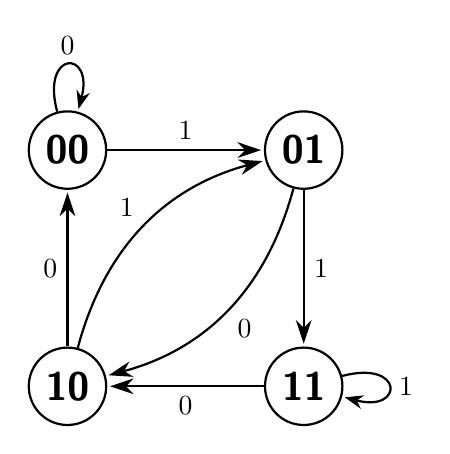
\begin{tikzpicture}[
      > = Stealth,
      shorten > = 1pt,
      auto,
      node distance = 3cm,
      thick,
      main node/.style = {circle, draw, font=\sffamily\Large\bfseries}
  ]
  % Define the vertices (nodes)
  \node[main node] (00) at (0,3) {00};
  \node[main node] (01) at (3,3) {01};
  \node[main node] (10) at (0,0) {10};
  \node[main node] (11) at (3,0) {11};

  % Define the edges with labels
  % From 00
  \path[->] (00) edge[loop above] node {0} (00);
  \path[->] (00) edge node {1} (01);

  % From 01
  \path[->] (01) edge[bend left] node {0} (10);
  \path[->] (01) edge node {1} (11);

  % From 10
  \path[->] (10) edge node {0} (00);
  \path[->] (10) edge[bend left] node {1} (01);

  % From 11
  \path[->] (11) edge node {0} (10);
  \path[->] (11) edge[loop right] node {1} (11);
  \end{tikzpicture}

  {\centering
\small Figure 41:De Bruijn Graph $B(2,3)$. This directed graph has 4 vertices representing all 2-bit sequences, and 8 edges labeled by the appended bit. An Eulerian circuit on this graph yields a de Bruijn sequence of order~3 over a binary alphabet. \par}
\end{figure}

\begin{figure}[ht]
{\centering
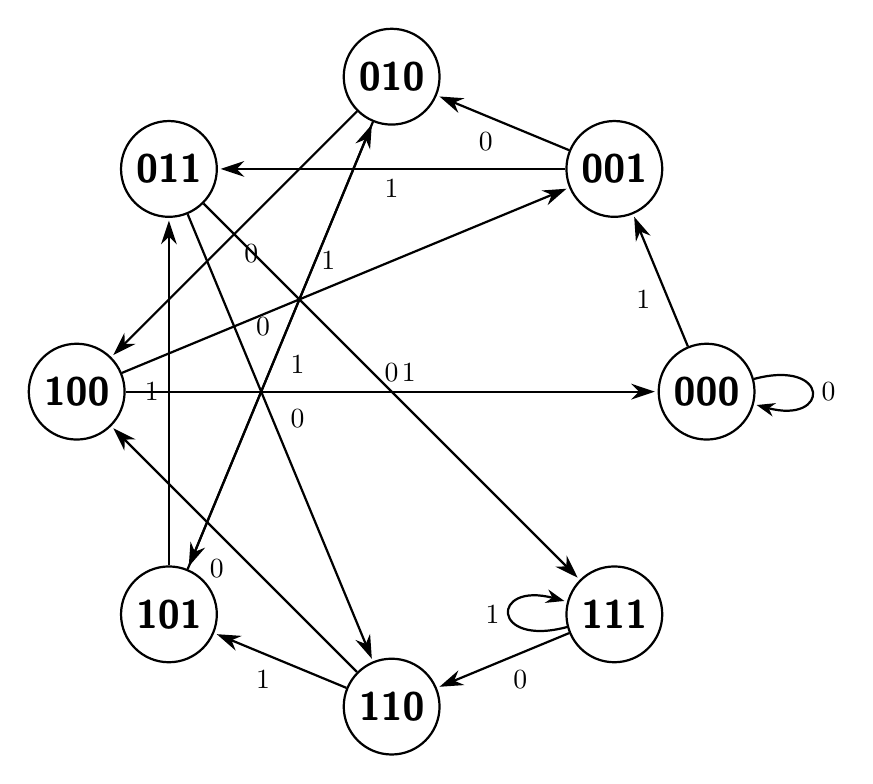
\begin{tikzpicture}[
    > = Stealth,
    shorten > = 1pt,
    auto,
    thick,
    main node/.style = {circle, draw, font=\sffamily\Large\bfseries}
]
% Define vertices in an octagonal arrangement
\def\radius{4}
\node[main node] (000) at ({\radius*cos(0)},{\radius*sin(0)}) {000};
\node[main node] (001) at ({\radius*cos(45)},{\radius*sin(45)}) {001};
\node[main node] (010) at ({\radius*cos(90)},{\radius*sin(90)}) {010};
\node[main node] (011) at ({\radius*cos(135)},{\radius*sin(135)}) {011};
\node[main node] (100) at ({\radius*cos(180)},{\radius*sin(180)}) {100};
\node[main node] (101) at ({\radius*cos(225)},{\radius*sin(225)}) {101};
\node[main node] (110) at ({\radius*cos(270)},{\radius*sin(270)}) {110};
\node[main node] (111) at ({\radius*cos(315)},{\radius*sin(315)}) {111};

% Define the edges with labels
% From 000
\path[->] (000) edge[loop right] node {0} (000);
\path[->] (000) edge node {1} (001);

% From 001
\path[->] (001) edge node {0} (010);
\path[->] (001) edge node {1} (011);

% From 010
\path[->] (010) edge node {0} (100);
\path[->] (010) edge node {1} (101);

% From 011
\path[->] (011) edge node {0} (110);
\path[->] (011) edge node {1} (111);

% From 100
\path[->] (100) edge node {0} (000);
\path[->] (100) edge node {1} (001);

% From 101
\path[->] (101) edge node {0} (010);
\path[->] (101) edge node {1} (011);

% From 110
\path[->] (110) edge node {0} (100);
\path[->] (110) edge node {1} (101);

% From 111
\path[->] (111) edge node {0} (110);
\path[->] (111) edge[loop left] node {1} (111);

\end{tikzpicture}
\par}
{\centering
\small Figure 42: De Bruijn Graph $B(2,4)$. This directed graph has 8 vertices representing all possible 3-bit binary sequences (000 through 111). Each edge is labeled with the bit (0 or 1) that is appended when transitioning between states. The graph has 16 edges in total, and a De Bruijn sequence $B(2,4)$ corresponds to an Eulerian circuit traversing all edges exactly once.
\par}
\end{figure}
\begin{lemma}[Connection to Eulerian Circuits]
A De Bruijn sequence $B(k,n)$ corresponds exactly to an Eulerian circuit in the De Bruijn graph $B(k,n-1)$.
\end{lemma}
\begin{proof}[Proof sketch]
Each edge in the De Bruijn graph $B(k,n-1)$ represents the transition from one $(n-1)$-length sequence to another by appending a symbol and removing the first symbol. Following an Eulerian circuit through all edges generates each possible $n$-length sequence exactly once, which is precisely the definition of a De Bruijn sequence.
\end{proof}
\begin{lemma}[Fundamental Property of De Bruijn Graphs]
For any alphabet size $k$ and order $n$, the De Bruijn graph $B(k,n)$ has exactly $k^n$ vertices and $k^{n+1}$ edges.
\end{lemma}
\begin{proof}
Each vertex in $B(k,n)$ represents a sequence of $n$ symbols from an alphabet of size $k$, giving exactly $k^n$ possible vertices. From each vertex, there are $k$ possible transitions (one for each symbol in the alphabet), resulting in exactly $k \cdot k^n = k^{n+1}$ edges.
\end{proof}
\begin{lemma}[Connection to Eulerian Circuits]
A De Bruijn sequence $B(k,n)$ corresponds exactly to an Eulerian circuit in the De Bruijn graph $B(k,n-1)$.
\end{lemma}
\begin{proof}[Proof sketch]
Each edge in the De Bruijn graph $B(k,n-1)$ represents the transition from one $(n-1)$-length sequence to another by appending a symbol and removing the first symbol. Following an Eulerian circuit through all edges generates each possible $n$-length sequence exactly once, which is precisely the definition of a De Bruijn sequence.
\end{proof}
\begin{remark}[Relationship to Universal Cycles]
De Bruijn sequences are a special case of universal cycles, which are cyclic sequences where each object from a set appears exactly once as a consecutive substring. When the objects are all possible $n$-tuples from a $k$-symbol alphabet, the universal cycle is precisely a De Bruijn sequence of order $n$.
\end{remark}
\begin{theorem}[Line Graph Relationship]
The De Bruijn graph $B(k,n+1)$ is isomorphic to the line graph of $B(k,n)$.
\end{theorem}

\begin{proof}
In the line graph of $B(k,n)$, each vertex corresponds to an edge in $B(k,n)$. An edge in $B(k,n)$ represents a transition from an $n$-length sequence to another by appending a symbol and removing the first symbol, which results in an $(n+1)$-length sequence. This exactly corresponds to a vertex in $B(k,n+1)$. Two vertices in the line graph are adjacent if their corresponding edges in $B(k,n)$ form a directed path of length 2, which precisely matches the adjacency condition in $B(k,n+1)$.
\end{proof}
\begin{theorem}[Shift Register Implementation]
Every binary De Bruijn sequence of order $n$ can be generated by a linear feedback shift register of length $n$ with an appropriate feedback function.
\end{theorem}

\begin{proof}[Proof outline]
Consider an $n$-bit shift register with bits $(b_1, b_2, \ldots, b_n)$. For each state of the register, we compute the next bit $b_{n+1}$ using a feedback function $f(b_1, b_2, \ldots, b_n)$. This bit is then shifted into the register, and $b_1$ is discarded.

For a De Bruijn sequence, we need a feedback function $f$ such that the shift register cycles through all $2^n$ possible states before repeating. This can be achieved by defining $f$ such that:

1. For the state $(0, 0, \ldots, 0)$, $f$ outputs 1 (to avoid the cycle containing only zeros)
2. For all other states, $f$ is chosen strategically to ensure a maximal cycle

One such function for binary De Bruijn sequences is:
\begin{center}
$f(b_1, b_2, \ldots, b_n) = b_1 \oplus b_2 \oplus \cdots \oplus b_{n-1} \oplus (b_n \lor 1)$
\end{center}
where $\oplus$ is XOR and $\lor$ is OR. This produces a modified maximum-length sequence that includes all $2^n$ possible states.
\end{proof}
\pagebreak
\pagebreak
\clearpage
\subsection{Chapter 2 Exercises}
\subsubsection{Easy Problems: Eulerian Graphs}
\begin{enumerate}
    \item Determine whether the following graph is Eulerian, semi-Eulerian, or neither:
    A graph with vertices $\{A, B, C, D, E\}$ and edges $\{(A,B), (B,C), (C,D), (D,E), (E,A), (A,C), (C,E)\}$
    
    \item Prove that a connected graph has an Eulerian path if and only if it has exactly 0 or 2 vertices with odd degree.
    
    \item Construct a simple graph with 6 vertices that has an Eulerian circuit. How many edges must such a graph have at minimum?
    
    \item Given a connected graph where all vertices have even degree, prove that it has an Eulerian circuit.

    
\end{enumerate}

\subsubsection{Medium Problems: Eulerian Graphs}
\begin{enumerate}[resume]
    \item A village has 7 bridges connecting different areas. Is it possible to walk through the village crossing each bridge exactly once? If so, find such a path. If not, explain why.
    
    \item Show that if $G$ is a connected graph where every vertex has even degree, then removing any edge results in a graph that has an Eulerian path but not an Eulerian circuit.
    
    \item Given a connected graph $G$ with $2k$ vertices of odd degree ($k \geq 1$), what is the minimum number of paths needed to cover all edges of $G$ exactly once?
    
    \item Prove that if $G$ is a connected graph with exactly two vertices of odd degree, say $u$ and $v$, then there exists an Eulerian path from $u$ to $v$.
\end{enumerate}

\subsubsection{Hard Problems: Eulerian Graphs}
\begin{enumerate}[resume]
    \item Prove that a connected graph $G$ has an Eulerian circuit if and only if its edge set can be partitioned into simple cycles.
    
    \item Consider a complete graph $K_n$. For which values of $n$ does $K_n$ have an Eulerian circuit? Provide a proof for your answer.
    
    \item Let $G$ be a connected graph with an even number of edges. Prove that the edges of $G$ can be partitioned into paths of length 2 if and only if $G$ has no vertices of odd degree.
    
    \item For a connected graph $G$, let $o(G)$ denote the number of vertices with odd degree. If $G_1, G_2, \ldots, G_k$ are the connected components of $G$, prove that $\sum_{i=1}^{k} o(G_i)$ is even.
\end{enumerate}

\subsubsection{Easy Problems: De Bruijn Sequences}
\begin{enumerate}[resume]
    \item Construct a binary De Bruijn sequence of order 3 (i.e., a circular sequence where every possible 3-length binary string appears exactly once as a substring).
    
    \item How many distinct binary De Bruijn sequences of order 4 exist? Explain your reasoning.
    
    \item For a ternary alphabet $\{0,1,2\}$, what is the length of a De Bruijn sequence of order 2? List all possible substrings that must appear exactly once.
    
    
\end{enumerate}

\subsubsection{Medium Problems: De Bruijn Sequences}
\begin{enumerate}[resume]
    \item Prove that for any alphabet of size $k$, a De Bruijn sequence of order $n$ has length $k^n$.
    
    \item Construct a De Bruijn sequence of order 2 for an alphabet of size 3. Then describe an algorithm to generate such sequences for any alphabet size.
    
    \item Show how to construct a De Bruijn sequence of order $n+1$ from a De Bruijn sequence of order $n$.
    
    \item Given a binary De Bruijn sequence of order 4, describe how many different such sequences exist and explain an algorithm to generate them.
\end{enumerate}

\subsubsection{Hard Problems: De Bruijn Sequences}
\begin{enumerate}[resume]
    \item Prove that any De Bruijn sequence of order $n$ for an alphabet of size $k$ can be represented as an Eulerian circuit in a directed graph with $k^{n-1}$ vertices.
    
    \item Given a De Bruijn sequence of order $n$ over alphabet $\{0,1\}$, describe an algorithm to find the position of any $n$-length binary string within the sequence without examining the entire sequence.
    
    \item Prove that for any binary De Bruijn sequence of order $n$, there exists a corresponding binary necklace of length $2^n - 1$.
\end{enumerate}

\subsubsection{Easy Problems: De Bruijn Graphs}
\begin{enumerate}[resume]
    \item Draw the De Bruijn Graph of order 1 for the binary alphabet $\{0,1\}$. How many vertices and edges does it have?
    
    \item For a ternary alphabet $\{0,1,2\}$, construct the De Bruijn Graph of order 1. How many vertices and edges does it have?
    \item Draw the De Bruijn Graph of order 2 for the binary alphabet $\{0,1\}$. Then trace a path through this diagram that generates a De Bruijn sequence of order 3.
    
    \item Draw a binary De Bruijn Graph of order 1 (with vertices $0$ and $1$). Then draw the corresponding De Bruijn Graph of order 2 using the line graph construction.
    
    \item Draw a De Bruijn Graph for a ternary alphabet $\{0,1,2\}$ of order 1. Find an Eulerian circuit in this diagram and write down the corresponding De Bruijn sequence.
\end{enumerate}

\subsubsection{Medium Problems: De Bruijn Graphs}
\begin{enumerate}[resume]
    \item Prove that the De Bruijn Graph $B(k,n)$ has $k^n$ vertices and $k^{n+1}$ edges.
    
    \item Consider a modified De Bruijn graph where certain transitions are forbidden. Specifically, in a binary De Bruijn graph of order 3, transitions to states containing "$111$" are prohibited. Is it still possible to find an Eulerian path in this modified diagram? If so, construct one. If not, explain why.
\end{enumerate}

\subsubsection{Hard Problems: De Bruijn Graphs}
\begin{enumerate}[resume]
    \item Let $B(k,n)$ be the De Bruijn graph of order $n$ over an alphabet of size $k$. Prove that the line graph of $B(k,n)$ is isomorphic to $B(k,n+1)$.
    
    \item For a De Bruijn Graph $B(2,n)$, determine the chromatic number of the underlying undirected graph and prove your answer.
\end{enumerate}

\clearpage

\section{Hamiltonian Graphs}
\subsection{Hamiltonian Walks, Paths, Cycles}

\begin{definition}[Hamiltonian Cycle]
A Hamiltonian cycle in a graph $G$ is a cycle that visits each vertex of $G$ exactly once (except for the starting vertex, which is also the ending vertex). Equivalently, a Hamiltonian cycle is a spanning cycle of the graph, meaning $V(C) = V(G)$. A graph is called Hamiltonian if it contains a Hamiltonian cycle.
\end{definition}

\begin{definition}[Hamiltonian Path]
A Hamiltonian path in a graph $G$ is a path that visits each vertex of $G$ exactly once. Equivalently, a Hamiltonian path is a spanning path in the graph, meaning $V(P) = V(G)$. A graph is called traceable if it contains a Hamiltonian path.
\end{definition}

\begin{figure}[H]
    \centering
    \begin{tikzpicture}[
        vertex/.style={circle, draw=black, thick, fill=blue!15, minimum size=0.8cm, font=\bfseries},
        normaledge/.style={draw, thick, black!30},
        pathedge/.style={draw, very thick, red!80!black, -latex}
    ]
        % Vertices
        \node[vertex] (A) at (0,3) {$A$};
        \node[vertex] (B) at (2,4) {$B$};
        \node[vertex] (C) at (4,3) {$C$};
        \node[vertex] (D) at (3,1) {$D$};
        \node[vertex] (E) at (1,1) {$E$};
        
        % All edges (grayed out)
        \draw[normaledge] (A) -- (B);
        \draw[normaledge] (B) -- (C);
        \draw[normaledge] (C) -- (D);
        \draw[normaledge] (D) -- (E);
        \draw[normaledge] (E) -- (A);
        \draw[normaledge] (A) -- (C);
        \draw[normaledge] (B) -- (D);
        
        % Hamiltonian path (highlighted)
        \draw[pathedge] (A) -- (B);
        \draw[pathedge] (B) -- (C);
        \draw[pathedge] (C) -- (D);
        \draw[pathedge] (D) -- (E);
        
        % Label
        \node[align=center, font=\sffamily\bfseries] at (2,0) {Hamiltonian Path: $A \to B \to C \to D \to E$};
    \end{tikzpicture}
    
    \vspace{0.2cm}
    \begin{center}
    \small Figure 43: Example of a Hamiltonian path. The red path visits every vertex of the graph exactly once, making it a Hamiltonian path. Unlike Eulerian paths which must traverse every edge exactly once, a Hamiltonian path must visit every vertex exactly once.
    \end{center}
\end{figure}

\begin{figure}[H]
    \centering
    \begin{tikzpicture}[
        vertex/.style={circle, draw=black, thick, fill=blue!15, minimum size=0.8cm, font=\bfseries},
        normaledge/.style={draw, thick, black!30},
        cycleedge/.style={draw, very thick, red!80!black, -latex}
    ]
        % Vertices
        \node[vertex] (A) at (0,3) {$A$};
        \node[vertex] (B) at (2,4) {$B$};
        \node[vertex] (C) at (4,3) {$C$};
        \node[vertex] (D) at (3,1) {$D$};
        \node[vertex] (E) at (1,1) {$E$};
        
        % All edges (grayed out)
        \draw[normaledge] (A) -- (B);
        \draw[normaledge] (B) -- (C);
        \draw[normaledge] (C) -- (D);
        \draw[normaledge] (D) -- (E);
        \draw[normaledge] (E) -- (A);
        \draw[normaledge] (A) -- (C);
        \draw[normaledge] (B) -- (E);
        
        % Hamiltonian cycle (highlighted)
        \draw[cycleedge] (A) -- (B);
        \draw[cycleedge] (B) -- (C);
        \draw[cycleedge] (C) -- (D);
        \draw[cycleedge] (D) -- (E);
        \draw[cycleedge] (E) -- (A);
        
        % Label
        \node[align=center, font=\sffamily\bfseries] at (2,0) {Hamiltonian Cycle: $A \to B \to C \to D \to E \to A$};
    \end{tikzpicture}
    
    \vspace{0.2cm}
    \begin{center}
    \small Figure 44: Example of a Hamiltonian cycle. The red cycle visits every vertex of the graph exactly once before returning to the starting vertex, forming a closed loop.
    \end{center}
\end{figure}
\begin{lemma}[Difference Between Hamiltonian and Eulerian]
There exists no known simple necessary and sufficient condition for a graph to be Hamiltonian, unlike Eulerian graphs which can be characterized by the parity of vertex degrees.
\end{lemma}

\begin{figure}[H]
    \centering
    \begin{tikzpicture}[
        vertex/.style={circle, draw=black, thick, fill=blue!15, minimum size=0.8cm, font=\bfseries},
        smallvertex/.style={circle, draw=black, thick, fill=blue!15, minimum size=0.7cm, font=\small},
        normaledge/.style={draw, thick, black!70},
        cycleedge/.style={draw, very thick, red!80!black, -latex}
    ]
        % Non-Hamiltonian graph (Petersen graph)
        \begin{scope}[shift={(-5,0)}, scale=0.9]
            % Outer vertices
            \foreach \i in {1,...,5} {
                \node[smallvertex] (A\i) at ({90+72*(\i-1)}:2.2) {$v_{\i}$};
            }
            
            % Inner vertices
            \foreach \i in {1,...,5} {
                \node[smallvertex] (B\i) at ({90+72*(\i-1)}:1.1) {$u_{\i}$};
            }
            
            % Outer edges
            \foreach \i in {1,...,5} {
                \pgfmathtruncatemacro{\j}{mod(\i,5)+1}
                \draw[normaledge] (A\i) -- (A\j);
            }
            
            % Spoke edges
            \foreach \i in {1,...,5} {
                \draw[normaledge] (A\i) -- (B\i);
            }
            
            % Inner star edges
            \foreach \i in {1,...,5} {
                \pgfmathtruncatemacro{\j}{mod(\i+1,5)+1}
                \draw[normaledge] (B\i) -- (B\j);
            }
            
            % Label
            \node[text width=4cm, align=center, font=\bfseries] at (0,-3) {Non-Hamiltonian Graph\\(Petersen Graph)};
        \end{scope}
        
        % Hamiltonian graph (Complete graph K5)
        \begin{scope}[shift={(5,0)}]
            % Vertices of a complete graph K5 with regular spacing
            \foreach \i/\ilabel in {1/A, 2/B, 3/C, 4/D, 5/E} {
                \node[vertex] (K\i) at ({90+72*(\i-1)}:1.7) {$\ilabel$};
            }
            
            % All edges of K5
            \foreach \i in {1,...,5} {
                \foreach \j in {1,...,5} {
                    \ifnum\i=\j\else
                        \ifnum\i<\j
                            \draw[normaledge] (K\i) -- (K\j);
                        \fi
                    \fi
                }
            }
            
            % One possible Hamiltonian cycle with directional arrows
            \draw[cycleedge] (K1) -- (K2);
            \draw[cycleedge] (K2) -- (K3);
            \draw[cycleedge] (K3) -- (K4);
            \draw[cycleedge] (K4) -- (K5);
            \draw[cycleedge] (K5) -- (K1);
            
            % Label
            \node[text width=4cm, align=center, font=\bfseries] at (0,-3) {Hamiltonian Graph\\(Complete Graph $K_5$)};
        \end{scope}
    \end{tikzpicture}
    
    \begin{center}
    \small Figure 45: Comparison of a non-Hamiltonian graph (Petersen graph) and a Hamiltonian graph (complete graph $K_5$). The complete graph contains a Hamiltonian cycle (shown with red arrows) that visits every vertex exactly once before returning to the starting vertex.
    \end{center}
\end{figure}

\begin{theorem}
The Petersen graph is not Hamiltonian.
\end{theorem}

\begin{proof}
We present a proof by contradiction. Suppose that the Petersen graph contains a Hamiltonian cycle $C$.

Let us recall that the Petersen graph has 10 vertices and 15 edges, where each vertex has exactly 3 neighbors. The graph can be constructed as follows:
\begin{itemize}
    \item Create an outer 5-cycle with vertices labeled $\{v_1, v_2, v_3, v_4, v_5\}$
    \item Create an inner 5-pointed star with vertices labeled $\{u_1, u_2, u_3, u_4, u_5\}$
    \item Connect each outer vertex $v_i$ to the corresponding inner vertex $u_i$
\end{itemize}

Now, if a Hamiltonian cycle $C$ exists, it must use exactly 10 edges of the graph to visit all 10 vertices exactly once. Since the Petersen graph has 15 edges in total, the cycle $C$ omits exactly 5 edges.

Let us classify the edges of the Petersen graph into three types:
\begin{enumerate}
    \item Type A: The 5 edges of the outer 5-cycle $\{v_1, v_2, v_3, v_4, v_5\}$
    \item Type B: The 5 "spoke" edges connecting $v_i$ to $u_i$ for $i \in \{1,2,3,4,5\}$
    \item Type C: The 5 edges of the inner star connecting $u_i$ to $u_{i \pm 2}$ (with indices taken modulo 5)
\end{enumerate}

For a Hamiltonian cycle to exist, it must use exactly 2 edges incident to each vertex (entering and exiting). Since each vertex has degree 3, exactly one edge at each vertex must be omitted from the cycle. This means that the 5 omitted edges form a perfect matching (or 1-factor) of the Petersen graph.

However, we can verify that no perfect matching can consist entirely of edges of a single type:
\begin{itemize}
    \item Type A edges form a 5-cycle, not a matching
    \item Type B edges form a perfect matching, but if all Type B edges were omitted, the outer and inner vertices would be disconnected, making a Hamiltonian cycle impossible
    \item Type C edges form a 5-cycle among inner vertices, not a matching
\end{itemize}

Therefore, the 5 omitted edges must include edges of different types. But this creates a problem: if we omit some edges of each type, we can verify (by exhaustive case analysis or by using the symmetry of the graph) that it's impossible to form a Hamiltonian cycle with the remaining edges.

For example, if we omit 2 Type A edges, 2 Type B edges, and 1 Type C edge, then some vertex will be either isolated or have both its cycle edges from the same component (inner or outer), making it impossible to form a cycle that visits all vertices.

This contradiction proves that the Petersen graph cannot contain a Hamiltonian cycle.
\end{proof}

% Complete Graph definition
\begin{remark}[Complete Graphs]
Recall that a complete graph $K_n$, introduced in Chapter 1, is a simple graph where every pair of vertices is connected by an edge. This property makes complete graphs particularly important for studying Hamiltonian cycles.
\end{remark}

\begin{figure}[H]
    \centering
    \begin{tikzpicture}[
        vertex/.style={circle, draw=black, thick, fill=blue!15, minimum size=0.8cm, font=\bfseries},
        edge/.style={draw, thick}
    ]
        % First diagram: K4
        \begin{scope}[shift={(-4,0)}]
            % Vertices with better layout
            \node[vertex] (A) at (0,2) {$1$};
            \node[vertex] (B) at (2,2) {$2$};
            \node[vertex] (C) at (2,0) {$3$};
            \node[vertex] (D) at (0,0) {$4$};
            
            % Edges - all pairs are connected
            \draw[edge] (A) -- (B);
            \draw[edge] (A) -- (C);
            \draw[edge] (A) -- (D);
            \draw[edge] (B) -- (C);
            \draw[edge] (B) -- (D);
            \draw[edge] (C) -- (D);
            
            % Title and properties
            \node[align=center, font=\sffamily\bfseries] at (1,-1.5) {$K_4$: Complete graph\\on 4 vertices};
            \node[align=center, text=blue!80!black, font=\sffamily] at (1,-2.5) {Each vertex has degree 3 $(n-1)$\\Total of 6 edges $\binom{4}{2}$};
        \end{scope}
        
        % Second diagram: K5
        \begin{scope}[shift={(4,0)}]
            % Vertices with even spacing
            \foreach \i in {1,...,5} {
                \node[vertex] (K\i) at ({90+72*(\i-1)}:2) {$\i$};
            }
            
            % Edges - all pairs are connected
            \foreach \i in {1,...,5} {
                \foreach \j in {\i,...,5} {
                    \ifnum\i=\j\else
                        \draw[edge] (K\i) -- (K\j);
                    \fi
                }
            }
            
            % Title and properties
            \node[align=center, font=\sffamily\bfseries] at (0,-3) {$K_5$: Complete graph\\on 5 vertices};
            \node[align=center, text=blue!80!black, font=\sffamily] at (0,-4) {Each vertex has degree 4 $(n-1)$\\Total of 10 edges $\binom{5}{2}$};
        \end{scope}
    \end{tikzpicture}
    
    \begin{center}
    \small Figure 46: Examples of complete graphs $K_4$ and $K_5$. In a complete graph, every pair of distinct vertices is connected by exactly one edge. Each vertex has degree $n-1$, and the total number of edges is $\binom{n}{2} = \frac{n(n-1)}{2}$.
    \end{center}
\end{figure}

\begin{corollary}
Every complete graph $K_n$ with $n \geq 3$ is Hamiltonian.
\end{corollary}
\begin{remark}[Applications of Hamiltonian Cycles in Complete Graphs]
Complete graphs have numerous practical applications involving Hamiltonian cycles. In particular, the Traveling Salesperson Problem (TSP) can be modeled using complete graphs, where vertices represent cities and edges represent paths between them, with weights indicating distances. Finding a minimum-weight Hamiltonian cycle in this complete graph corresponds to finding the optimal route for the salesperson.
\end{remark}


\begin{theorem}[NP-Completeness of Hamiltonian Cycle Problem]
The problem of determining whether a given graph contains a Hamiltonian cycle is NP-complete. However, for complete graphs, the existence of a Hamiltonian cycle is guaranteed for $n \geq 3$, though finding the minimum-weight Hamiltonian cycle remains NP-hard.
\end{theorem}

\begin{example}[Number of Hamiltonian Cycles]
The number of distinct Hamiltonian cycles in a complete graph $K_n$ is $\frac{(n-1)!}{2}$. For example:
\begin{itemize}
    \item $K_3$ has exactly 1 Hamiltonian cycle (up to equivalence)
    \item $K_4$ has exactly 3 Hamiltonian cycles
    \item $K_5$ has exactly 12 Hamiltonian cycles
    \item $K_{10}$ has approximately 181,440 distinct Hamiltonian cycles
\end{itemize}
This rapid growth illustrates why brute-force approaches to the TSP quickly become impractical as the number of vertices increases.
\end{example}
\subsection{Dirac's Theorem}

\begin{theorem}[Dirac, 1952]
Let $G$ be a simple graph with $n \geq 3$ vertices. If every vertex has degree at least $\frac{n}{2}$ (equivalently, if the minimum degree $\delta(G) \geq \frac{n}{2}$), then $G$ contains a Hamiltonian cycle (i.e., $G$ is Hamiltonian).
\end{theorem}
\begin{proof}
Suppose the theorem is false. So there exists an $n$-vertex graph $G$ with minimum degree at least $\frac{n}{2}$ and no Hamiltonian cycle.
Let $G$ be a maximal counterexample to the theorem, i.e., with as many edges as possible.
Note: $K_n$ is Hamiltonian, so $G \neq K_n$. Thus, if $\{u,v\} \not\in E(G)$, then $G + \{u,v\}$ is Hamiltonian.
So $G + \{u,v\}$ has a Hamiltonian path from $u$ to $v$.
For a vertex $w \in V \setminus \{u,v\}$, let $w^+$ be the vertex after $w$ on the path from $u$ to $v$.
Let $S = \{w^+ : w \in N_G(u)\}$.
We want $N_G(u) \cap N_G(v) \neq \emptyset$.
Note that $N_G(u) \cup N_G(v) \subseteq V \setminus \{u,v\}$, so $|N_G(u) \cup N_G(v)| \leq n-2$.
Since $|N_G(u)| \geq \frac{n}{2}$ and $|N_G(v)| \geq \frac{n}{2}$, we have:
\begin{align*}
|N_G(u) \cap N_G(v)| &= |N_G(u)| + |N_G(v)| - |N_G(u) \cup N_G(v)|\\
&\geq \frac{n}{2} + \frac{n}{2} - (n-2)\\
&= 2
\end{align*}
Therefore, there exists $w \in N_G(u) \cap N_G(v)$.
Now let $C$ be the cycle consisting of the edges $\{u,w\}$, $\{w,v\}$, and the path from $v$ to $u$ in the Hamiltonian path of $G + \{u,v\}$.
This creates a Hamiltonian cycle in $G$, a contradiction.
\end{proof}
\begin{remark}[Algorithmic Verification]
Dirac's condition is particularly valuable because it can be verified in $O(n)$ time by simply checking the minimum degree of the graph, whereas determining if a general graph has a Hamiltonian cycle is NP-complete.
\end{remark}
\begin{algorithm}
\caption{Verify Dirac's Condition}
\begin{algorithmic}[1]
\Require Graph $G = (V, E)$ with $n \geq 3$ vertices
\State $\text{min\_degree} \gets n$
\For{each $v \in V$}
    \State $\text{min\_degree} \gets \min(\text{min\_degree}, |N(v)|)$
\EndFor
\State $\text{dirac\_satisfied} \gets \text{min\_degree} \geq \lceil n/2 \rceil$
\State \Return $\text{dirac\_satisfied}$
\end{algorithmic}
\end{algorithm}

\begin{remark}[Algorithmic Efficiency]
The algorithm's time complexity is $O(n)$ assuming the graph is represented with adjacency lists and degree information is readily available. This is significantly more efficient than directly testing for Hamiltonicity, which is an NP-complete problem.
\end{remark}

\begin{remark}[Sufficiency vs. Necessity]
Dirac's condition is sufficient but not necessary for a graph to be Hamiltonian. Many graphs with minimum degree less than $n/2$ still contain Hamiltonian cycles.
\end{remark}

\begin{theorem}[Disjoint Union Property]
If $G_1$ and $G_2$ are two graphs that satisfy Dirac's condition individually, their disjoint union $G_1 \cup G_2$ does not necessarily satisfy Dirac's condition, highlighting that Hamiltonicity is not preserved under disjoint union.
\end{theorem}

\begin{remark}[Implementation Note]
When implementing this algorithm, special care should be taken with disconnected graphs, as no disconnected graph can have a Hamiltonian cycle regardless of minimum degree.
\end{remark}

\begin{lemma}[Approximating Hamiltonicity]
When $\delta(G) \geq \frac{n}{2} - \epsilon$ for small $\epsilon$, even though Dirac's condition isn't satisfied, the graph may still contain a path or cycle covering most vertices.
\end{lemma}
\newpage
\subsection{Visual Illustration of Dirac's Theorem Proof}

\begin{figure}[h!]
\centering
\begin{tikzpicture}[scale=1.2]
    % First diagram - original graph G
    \begin{scope}[xshift=-5cm]
        % Vertices
        \node[draw, circle, fill=gray!20] (u) at (0,0) {$u$};
        \node[draw, circle, fill=gray!20] (v) at (3,0) {$v$};
        
        % Other vertices
        \node[draw, circle, fill=gray!20] (w1) at (0.5,1.5) {$w_1$};
        \node[draw, circle, fill=gray!20] (w2) at (1.5,2) {$w_2$};
        \node[draw, circle, fill=gray!20] (w3) at (2.5,1.5) {$w_3$};
        \node[draw, circle, fill=gray!20] (w4) at (1.5,-1.5) {$w_4$};
        
        % Edges for u
        \draw (u) -- (w1);
        \draw (u) -- (w2);
        \draw (u) -- (w4);
        
        % Edges for v
        \draw (v) -- (w2);
        \draw (v) -- (w3);
        \draw (v) -- (w4);
        
        % Other edges
        \draw (w1) -- (w2);
        \draw (w2) -- (w3);
        \draw (w3) -- (w4);
        \draw (w4) -- (w1);
        
        % Note that u and v are not connected
        \node at (1.5,-2.5) {$G$ (with $\{u,v\} \not\in E(G)$)};
    \end{scope}
    
    % Second diagram - G + {u,v} with Hamiltonian path highlighted
    \begin{scope}[xshift=2cm]
        % Vertices
        \node[draw, circle, fill=gray!20] (u) at (0,0) {$u$};
        \node[draw, circle, fill=gray!20] (v) at (3,0) {$v$};
        
        % Other vertices
        \node[draw, circle, fill=gray!20] (w1) at (0.5,1.5) {$w_1$};
        \node[draw, circle, fill=gray!20] (w2) at (1.5,2) {$w_2$};
        \node[draw, circle, fill=gray!20] (w3) at (2.5,1.5) {$w_3$};
        \node[draw, circle, fill=gray!20] (w4) at (1.5,-1.5) {$w_4$};
        
        % Edges for u
        \draw (u) -- (w1);
        \draw (u) -- (w2);
        \draw (u) -- (w4);
        
        % Edges for v
        \draw (v) -- (w2);
        \draw (v) -- (w3);
        \draw (v) -- (w4);
        
        % Other edges
        \draw (w1) -- (w2);
        \draw (w2) -- (w3);
        \draw (w3) -- (w4);
        \draw (w4) -- (w1);
        
        % The edge {u,v} is added
        \draw[dashed] (u) -- (v) node[midway, above] {added};
        
        % Highlight a Hamiltonian path from u to v
        \draw[very thick, red, ->] (u) -- (w1);
        \draw[very thick, red, ->] (w1) -- (w2);
        \draw[very thick, red, ->] (w2) -- (w3);
        \draw[very thick, red, ->] (w3) -- (w4);
        \draw[very thick, red, ->] (w4) -- (v);
        
        \node at (1.5,-2.5) {$G + \{u,v\}$ with Hamiltonian path};
    \end{scope}
\end{tikzpicture}

\begin{center}
\small Figure 47: Illustration of the graph closure concept for Hamiltonicity. Left: Original graph $G$ where vertices $u$ and $v$ are not adjacent but have combined degree $\deg(u) + \deg(v) \geq n$. Right: After adding edge $\{u,v\}$ (shown as dashed), a Hamiltonian path (shown in red) exists from $u$ to $v$. The Bondy-Chvátal theorem proves that if such vertices have sufficient combined degree, adding the edge between them preserves the Hamiltonian property.
\end{center}
\end{figure}

\begin{figure}[h!]
\centering
\begin{tikzpicture}[scale=1.2]
    % Vertices
    \node[draw, circle, fill=gray!20] (u) at (0,0) {$u$};
    \node[draw, circle, fill=gray!20] (v) at (6,0) {$v$};
    
    % Other vertices on the path
    \node[draw, circle, fill=gray!20] (w1) at (1,1) {$w_1$};
    \node[draw, circle, fill=gray!20] (w2) at (2,1.5) {$w_2$};
    \node[draw, circle, fill=gray!20] (w3) at (3,1) {$w_3$};
    \node[draw, circle, fill=gray!20] (w4) at (4,1) {$w_4$};
    \node[draw, circle, fill=gray!20] (w5) at (5,1) {$w_5$};
    
    % Hamiltonian path from u to v
    \draw[thick] (u) -- (w1) -- (w2) -- (w3) -- (w4) -- (w5) -- (v);
    
    % Show that w2 is adjacent to both u and v
    \draw[blue, thick] (u) to[bend right] (w2) node[midway, below] {$\in E(G)$};
    \draw[blue, thick] (v) to[bend left] (w2) node[midway, below] {$\in E(G)$};
    
    % Highlight the common neighbor
    \node[draw, circle, fill=yellow!50, thick] at (2,1.5) {$w_2$};
    
    % Show the Hamiltonian cycle
    \draw[->, red, very thick, dashed] (u) to[bend right=30] (w2);
    \draw[->, red, very thick, dashed] (w2) to[bend right=30] (v);
    \draw[->, red, very thick] (v) -- (w5);
    \draw[->, red, very thick] (w5) -- (w4);
    \draw[->, red, very thick] (w4) -- (w3);
    \draw[->, red, very thick] (w3) -- (w1);
    \draw[->, red, very thick] (w1) -- (u);
    
    \node at (3,-1.5) {Finding a Hamiltonian cycle in $G$ using a common neighbor $w_2$};
\end{tikzpicture}

\begin{center}
\small Figure 48: Illustration of the "common neighbor" technique in the proof of Dirac's Theorem. When vertices $u$ and $v$ both have degree at least $n/2$, they must share at least one common neighbor (here $w_2$, highlighted in yellow). This allows us to construct a Hamiltonian cycle (red arrows) by rerouting the original path. The dashed red edges show how we can bypass the original path segment through $w_2$ to create a cycle that visits all vertices exactly once.
\end{center}
\end{figure}
\begin{theorem}[Closure Properties]
Let $G$ be a graph with $n$ vertices and let $c(G)$ be its closure. Then:
\begin{enumerate}
    \item $G$ is Hamiltonian if and only if $c(G)$ is Hamiltonian.
    \item If $G$ satisfies Dirac's condition (minimum degree $\delta(G) \geq n/2$), then $c(G)$ is a complete graph.
    \item The closure operation is uniquely defined, independent of the order in which edges are added.
\end{enumerate}
\end{theorem}
\begin{lemma}[Las Vergnas, 1972]
Let $G$ be a simple graph and let $u, v$ be non-adjacent vertices in $G$. If there exists a Hamiltonian path from $u$ to $v$ in $G$, then $G + \{u,v\}$ has a Hamiltonian cycle.
\end{lemma}
\begin{corollary}
If $G$ has a Hamiltonian path and its endpoints have degree sum at least $n$, then $G$ has a Hamiltonian cycle.
\end{corollary}
\begin{lemma}[Degree Sum of Common Neighbors]
Let $P = (v_1, v_2, \ldots, v_n)$ be a Hamiltonian path in a graph $G$. If $N(v_1) \cap N(v_n) \neq \emptyset$, then $G$ has a Hamiltonian cycle.
\end{lemma}
\subsection{Alternative Form of Dirac's Theorem}
\begin{theorem}[Dirac, 1952]
Let $G$ be a simple graph with $n \geq 3$ vertices. If every vertex has degree at least $\frac{n}{2}$ (equivalently, if the minimum degree $\delta(G) \geq \frac{n}{2}$), then $G$ contains a Hamiltonian cycle (i.e., $G$ is Hamiltonian).
\end{theorem}

\begin{lemma}
The degree condition in Dirac's theorem is tight, meaning that there exist graphs with minimum degree $\delta(G) = \frac{n}{2} - 1$ that are not Hamiltonian.
\end{lemma}
\begin{proof}[Proof Sketch]
If $G$ is not Hamiltonian, consider a longest path $P = (v_1, \ldots, v_k)$. Since $\deg(v_1) \geq \frac{n}{2}$ and $\deg(v_k) \geq \frac{n}{2}$, by the pigeonhole principle, there must exist vertices $v_i, v_{i+1}$ on $P$ such that $v_1v_{i+1}, v_kv_i \in E(G)$. This creates cycle $(v_1, \ldots, v_i, v_k, \ldots, v_{i+1}, v_1)$, contradicting $P$'s maximality.
\end{proof}
\begin{example}[Tightness of Dirac's Condition]
Consider the complete bipartite graph $K_{m,m+1}$ with $m \geq 2$. This graph has $n = 2m+1$ vertices, and each vertex has degree either $m$ or $m+1$. The minimum degree is $\delta(G) = m = \frac{n-1}{2} = \frac{n}{2} - \frac{1}{2}$, which is just below Dirac's threshold. This graph cannot contain a Hamiltonian cycle because any cycle must alternate between the two partite sets, which is impossible when the sets have different sizes.
\end{example}
\begin{remark}[Applications]
Dirac's Theorem provides a simple sufficient condition for Hamiltonicity that can be verified in linear time, making it valuable in network design applications where robustness requires the existence of a cycle visiting all nodes.
\end{remark}
\begin{remark}[Related Results]
Dirac's Theorem was generalized by Ore (1960), who showed that a graph is Hamiltonian if, for every pair of non-adjacent vertices $u$ and $v$, we have $\deg(u) + \deg(v) \geq n$. This is a strictly stronger result, as there exist graphs that satisfy Ore's condition but not Dirac's.
\end{remark}
\subsection{Examples of Dirac's Theorem}
\begin{example}[Minimum degree exactly $\frac{n}{2}$]
Consider a graph on $n = 6$ vertices where each vertex has degree exactly $\frac{n}{2} = 3$.
\end{example}
\begin{figure}[h!]
\begin{center}
\begin{tikzpicture}[scale=1.3]
    % Vertices arranged in a regular hexagon
    \foreach \i in {1,...,6} {
        \node[draw, circle, fill=gray!20] (v\i) at ({60*\i + 30}:1.5) {$v_\i$};
    }
    
    % Edges to ensure each vertex has degree 3
    \draw (v1) -- (v2) -- (v3) -- (v4) -- (v5) -- (v6) -- (v1);
    \draw (v1) -- (v4);
    \draw (v2) -- (v5);
    \draw (v3) -- (v6);
    
    % Highlight the Hamiltonian cycle
    \draw[red, very thick] (v1) -- (v2) -- (v3) -- (v4) -- (v5) -- (v6) -- (v1);
\end{tikzpicture}
\end{center}

\begin{center}
\small Figure 49: A 3-regular graph on 6 vertices that satisfies Dirac's condition. Each vertex has degree 3, which equals $n/2$. The red cycle highlights one of the Hamiltonian cycles in this graph. This example demonstrates that cubic (3-regular) graphs can be Hamiltonian when they meet the minimum degree threshold.
\end{center}
\end{figure}
\begin{lemma}[Cubic Graph Hamiltonicity]
Not all cubic graphs are Hamiltonian. The Petersen graph is a well-known 3-regular graph with 10 vertices that has no Hamiltonian cycle, demonstrating that regularity alone is insufficient for Hamiltonicity.
\end{lemma}
\newpage
\begin{figure}[h!]
\begin{center}
\begin{tikzpicture}[scale=1.2]
    % Left side vertices
    \node[draw, circle, fill=gray!20] (a1) at (0,2) {$a_1$};
    \node[draw, circle, fill=gray!20] (a2) at (0,1) {$a_2$};
    \node[draw, circle, fill=gray!20] (a3) at (0,0) {$a_3$};
    
    % Right side vertices
    \node[draw, circle, fill=gray!20] (b1) at (3,2) {$b_1$};
    \node[draw, circle, fill=gray!20] (b2) at (3,1) {$b_2$};
    \node[draw, circle, fill=gray!20] (b3) at (3,0) {$b_3$};
    
    % Edges connecting all vertices from left to right
    \foreach \i in {1,2,3} {
        \foreach \j in {1,2,3} {
            \draw (a\i) -- (b\j);
        }
    }
    
    % Highlight a Hamiltonian cycle
    \draw[red, very thick] (a1) -- (b1) -- (a2) -- (b2) -- (a3) -- (b3) -- (a1);
\end{tikzpicture}
\end{center}

\begin{center}
\small Figure 50: The complete bipartite graph $K_{3,3}$ with $n = 6$ vertices. Each vertex has degree exactly 3, which equals $\frac{n}{2}$, satisfying Dirac's condition. A Hamiltonian cycle is highlighted in red: $a_1 - b_1 - a_2 - b_2 - a_3 - b_3 - a_1$. This example illustrates that bipartite graphs can be Hamiltonian when they have equal-sized partitions.
\end{center}
\end{figure}

\begin{figure}[h!]
\begin{center}
\begin{tikzpicture}[scale=1.4]
    % Vertices arranged in a regular octagon
    \foreach \i in {1,...,8} {
        \node[draw, circle, fill=gray!20] (v\i) at ({45*\i - 22.5}:2) {$v_\i$};
    }
    
    % Outer cycle
    \draw (v1) -- (v2) -- (v3) -- (v4) -- (v5) -- (v6) -- (v7) -- (v8) -- (v1);
    
    % Additional edges to ensure each vertex has degree 4
    \draw (v1) -- (v5);
    \draw (v2) -- (v6);
    \draw (v3) -- (v7);
    \draw (v4) -- (v8);
    
    % Highlight a Hamiltonian cycle
    \draw[red, very thick] (v1) -- (v2) -- (v3) -- (v4) -- (v5) -- (v6) -- (v7) -- (v8) -- (v1);
\end{tikzpicture}
\end{center}

\begin{center}
\small Figure 51: A graph on $n = 8$ vertices where each vertex has degree exactly 4 ($= \frac{n}{2}$), precisely meeting Dirac's minimum degree condition. The graph contains a Hamiltonian cycle (highlighted in red) along the outer cycle. This example illustrates a family of graphs that can be constructed for any even $n$ where each vertex has degree exactly $\frac{n}{2}$ by connecting vertices to their opposites in a regular $n$-gon.
\end{center}
\end{figure}

\begin{definition}[Circulant Graph]
A circulant graph $\text{Circ}(n; S)$ is a graph with vertex set $\{0, 1, 2, \ldots, n-1\}$ and an edge between vertices $i$ and $j$ if and only if $|i - j| \equiv s \pmod{n}$ for some $s$ in the connection set $S \subseteq \{1, 2, \ldots, \lfloor n/2 \rfloor\}$. In other words, it's a graph where vertices are arranged in a circle, and each vertex is connected to specific vertices at fixed distances around the circle.
\end{definition}

\begin{definition}[Graph Toughness]
The toughness $t(G)$ of a graph $G$ is defined as:
\[t(G) = \min \left\{\frac{|S|}{c(G-S)} : S \subset V(G), c(G-S) > 1 \right\}\]
where $c(G-S)$ is the number of connected components in the graph after removing vertex set $S$. Intuitively, toughness measures how difficult it is to disconnect a graph by removing vertices.
\end{definition}

\begin{theorem}[Circulant Graphs and Hamiltonicity]
The graph shown in Figure 51 is an example of a circulant graph $\text{Circ}(8;\{1,4\})$. A circulant graph with $n$ vertices is Hamiltonian if and only if it is connected.
\end{theorem}

\begin{problem}
Show that in the graph of Figure 51, there are exactly 8 distinct Hamiltonian cycles. Hint: Count the cycles that use only the outer edges versus those that must use the "diagonal" connections.
\end{problem}

\begin{lemma}[Toughness of Regular Graphs]
The graph in Figure 51 has toughness exactly 1. In general, any $k$-regular graph with $k \geq 2$ has toughness at least $\frac{k}{2}$.
\end{lemma}


\begin{figure}[h!]
\begin{center}
\begin{tikzpicture}[scale=1.3]
    % Center vertex
    \node[draw, circle, fill=gray!20] (v1) at (0,0) {$v_1$};
    
    % Surrounding vertices
    \node[draw, circle, fill=gray!20] (v2) at (1.5,0) {$v_2$};
    \node[draw, circle, fill=gray!20] (v3) at (0,1.5) {$v_3$};
    \node[draw, circle, fill=gray!20] (v4) at (-1.5,0) {$v_4$};
    \node[draw, circle, fill=gray!20] (v5) at (0,-1.5) {$v_5$};
    
    % Edges
    \draw (v1) -- (v2);
    \draw (v1) -- (v3);
    \draw (v1) -- (v4);
    \draw (v1) -- (v5);
    \draw (v2) -- (v3);
    \draw (v3) -- (v4);
    \draw (v4) -- (v5);
    
    % Highlight that v5 has degree 1
    \node[draw, circle, fill=red!20, thick] at (0,-1.5) {$v_5$};
    \node at (0,-2.5) {$\deg(v_5) = 1 < \frac{n}{2} = 2.5$};
\end{tikzpicture}
\end{center}

\begin{center}
\small Figure 52: A graph that fails to satisfy Dirac's condition. This graph has $n = 5$ vertices, with vertex $v_5$ (highlighted in red) having degree 1, which is less than $\frac{n}{2} = 2.5$. The graph cannot contain a Hamiltonian cycle because any cycle including $v_5$ must use both its only edge (to $v_1$) as entry and exit, making it impossible to continue the cycle. This demonstrates why the minimum degree requirement in Dirac's theorem is necessary.
\end{center}
\end{figure}

\begin{lemma}[Connectivity Requirement]
If a graph $G$ has a Hamiltonian cycle, then $G$ is 2-connected.
\end{lemma}

\begin{proof}
Suppose $G$ has a Hamiltonian cycle $C$. If we remove any vertex $v$ from $G$, the cycle $C$ becomes a path that connects all remaining vertices. Therefore, $G-v$ is connected, meaning $G$ is 2-connected.
\end{proof}

\begin{theorem}[Pendant Vertices]
Any graph $G$ containing a pendant vertex cannot contain a Hamiltonian cycle.
\end{theorem}

\begin{proof}
Let $v$ be a pendant vertex in $G$ with its only neighbor $u$. Any cycle containing $v$ must use the edge $\{u,v\}$ twice: once to enter $v$ and once to exit. Since a cycle can use each edge at most once, this creates a contradiction.
\end{proof}

\begin{lemma}[Cut Vertices]
The vertex $v_1$ in Figure 52 is a cut vertex; hence no Hamiltonian cycle can exist in this graph.
\end{lemma}

\begin{proof}
Removing $v_1$ disconnects the graph into separate components containing $\{v_3,v_4\}$ and $\{v_2,v_5\}$. By Lemma 1, no Hamiltonian cycle can exist in a graph with a cut vertex.
\end{proof}

\begin{theorem}[Relaxed Degree Condition]
If $\delta(G) \geq \frac{n-1}{2}$, then $G$ is either Hamiltonian or isomorphic to $K_m + \overline{K}_m$ with $n = 2m-1$.
\end{theorem}

\begin{remark}[Wheel-Graph Relation]
The graph in Figure 52 can be viewed as a wheel graph $W_5$ with one edge removed. This removal causes the graph to fall just below Dirac's threshold, eliminating its Hamiltonian property.
\end{remark}

\begin{remark}[Dirac-Critical]
The graph is Dirac-critical: adding edge $\{v_2,v_5\}$ increases the minimum degree to $\lceil n/2 \rceil$ and makes the graph Hamiltonian.
\end{remark}

\begin{problem}
Determine which pairs of edges can be added to Figure 52 to meet Dirac's condition, and list all such possible pairs.
\end{problem}
\begin{lemma}[Dirac's Condition and Pendant Vertices]
Let $G$ be the graph in Figure 52 with a pendant vertex $v_5$ of degree 1. Then:
\begin{enumerate}
    \item $G$ fails Dirac's condition since $\deg(v_5) = 1 < \frac{n}{2} = 2.5$
    \item $G$ cannot contain a Hamiltonian cycle
    \item Adding the edge $\{v_2, v_5\}$ would increase $\deg(v_5)$ to 2, but this still falls short of Dirac's threshold
    \item $G$ requires at least two additional edges to satisfy Dirac's condition
\end{enumerate}
\end{lemma}

\begin{proof}
A Hamiltonian cycle requires each vertex to have degree at least 2, which $v_5$ fails to satisfy. Furthermore, $v_1$ is a cut vertex, dividing the graph into two components upon its removal, which prevents any Hamiltonian cycle from existing.
\end{proof}
\newpage
\subsection{Related Results and Extensions}
\subsubsection{Ore's Theorem}

\begin{theorem}[Ore's Theorem, 1960]
Let $G$ be a simple graph with $n \geq 3$ vertices. If for every pair of non-adjacent vertices $u$ and $v$ in $G$, 
\[\deg(u) + \deg(v) \geq n,\]
then $G$ is Hamiltonian.
\end{theorem}

\begin{figure}[h!]
\begin{center}
\begin{tikzpicture}[scale=1.2]
    % Vertices
    \node[draw, circle, fill=blue!20, minimum size=0.7cm] (A) at (0,1.5) {$u_1$};
    \node[draw, circle, fill=blue!20, minimum size=0.7cm] (B) at (1.5,1.5) {$u_2$};
    \node[draw, circle, fill=blue!20, minimum size=0.7cm] (C) at (2,-0.5) {$u_3$};
    \node[draw, circle, fill=blue!20, minimum size=0.7cm] (D) at (0,-0.5) {$u_4$};
    \node[draw, circle, fill=blue!20, minimum size=0.7cm] (E) at (-1,0.5) {$u_5$};
    
    % Edges
    \draw[thick] (A) -- (B);
    \draw[thick] (B) -- (C);
    \draw[thick] (C) -- (D);
    \draw[thick] (D) -- (E);
    \draw[thick] (E) -- (A);
    \draw[thick] (A) -- (C);
    \draw[thick] (B) -- (D);
    \draw[thick] (B) -- (E);
    
    % Hamiltonian cycle
    \draw[ultra thick, red, ->] (A) to[bend left=10] (B);
    \draw[ultra thick, red] (B) to[bend left=10] (C);
    \draw[ultra thick, red] (C) to[bend left=10] (D);
    \draw[ultra thick, red] (D) to[bend left=10] (E);
    \draw[ultra thick, red] (E) to[bend left=10] (A);
    
    % Missing edge
    \draw[dashed, blue, thick] (A) -- (D);
\end{tikzpicture}
\end{center}

\vspace{0.5cm}
{\centering
\small $\deg(u_1) = 3, \deg(u_2) = 4, \deg(u_3) = 3, \deg(u_4) = 3, \deg(u_5) = 3$
\par}

\vspace{0.3cm}
{\centering
\small For non-adjacent vertices $u_1$ and $u_4$: $\deg(u_1) + \deg(u_4) = 3 + 3 = 6 > 5 = n$
\par}

\begin{center}
\small Figure 52: A graph with $n = 5$ vertices satisfying Ore's condition. The red path shows a Hamiltonian cycle, and the blue dashed line indicates a non-adjacent vertex pair whose degree sum exceeds $n$.
\end{center}
\end{figure}
\begin{figure}[h!]
\begin{center}
\begin{tikzpicture}[scale=1.2]
    % Vertices
    \node[draw, circle, fill=blue!20, minimum size=0.7cm] (A) at (0,1.5) {$v_1$};
    \node[draw, circle, fill=blue!20, minimum size=0.7cm] (B) at (1.5,1.5) {$v_2$};
    \node[draw, circle, fill=blue!20, minimum size=0.7cm] (C) at (2,-0.5) {$v_3$};
    \node[draw, circle, fill=blue!20, minimum size=0.7cm] (D) at (0,-0.5) {$v_4$};
    \node[draw, circle, fill=blue!20, minimum size=0.7cm] (E) at (-1,0.5) {$v_5$};
    
    % Edges
    \draw[thick] (A) -- (B);
    \draw[thick] (B) -- (C);
    \draw[thick] (C) -- (D);
    \draw[thick] (A) -- (E);
    
    % Non-adjacent vertices with insufficient degree sum
    \draw[dashed, red, thick] (B) -- (E);
\end{tikzpicture}
\end{center}

\vspace{0.5cm}
{\centering
\small $\deg(v_1) = 2, \deg(v_2) = 2, \deg(v_3) = 2, \deg(v_4) = 1, \deg(v_5) = 1$
\par}

\vspace{0.3cm}
{\centering
\small For non-adjacent vertices $v_2$ and $v_5$: $\deg(v_2) + \deg(v_5) = 2 + 1 = 3 < 5 = n$
\par}

\vspace{0.3cm}
{\centering
\small No Hamiltonian cycle exists in this graph
\par}

\begin{center}
\small Figure 53: A graph with $n = 5$ vertices that fails both Dirac's and Ore's conditions. The red dashed line shows a non-adjacent vertex pair whose degree sum is less than $n$.
\end{center}
\end{figure}
\begin{lemma}[Ore's Condition and Path Graphs]
Let $P_n$ be a path graph with $n \geq 4$ vertices. Then:
\begin{enumerate}
    \item For any non-adjacent vertices $u$ and $v$ in $P_n$, $\deg(u) + \deg(v) \leq 4 < n$
    \item $P_n$ fails to satisfy Ore's condition
    \item The graph in Figure 53 contains a path $P_4$ as a subgraph $(v_2, v_3, v_4, v_5)$
    \item Adding any single edge to Figure 53 is insufficient to satisfy Ore's condition
\end{enumerate}
\end{lemma}

\begin{proof}
In any path graph $P_n$ with $n \geq 4$, the maximum degree of any vertex is 2. Consider any pair of non-adjacent vertices $u$ and $v$. Their degree sum is at most $2 + 2 = 4$, which is less than $n$. Thus, $P_n$ always fails Ore's condition and cannot be Hamiltonian. The graph in Figure 53 contains the path $(v_2, v_3, v_4, v_5)$ and exhibits similar properties, with vertices $v_4$ and $v_5$ having degree only 1, making it even further from satisfying Ore's condition.
\end{proof}
\subsubsection{Chvátal's Theorem}

\begin{theorem}[Chvátal, 1972]
Let $G$ be a simple graph with $n$ vertices and degree sequence $d_1 \leq d_2 \leq \ldots \leq d_n$. If for all $i < \frac{n}{2}$, 
\[d_i \leq i \implies d_{n-i} \geq n-i,\]
then $G$ is Hamiltonian.
\end{theorem}




\begin{figure}[h!]
\begin{center}
\begin{minipage}{0.48\textwidth}
\centering
\begin{tikzpicture}[scale=1]
    % Vertices
    \node[draw, circle, fill=green!20, minimum size=0.6cm] (A) at (90:1.5) {$a_1$};
    \node[draw, circle, fill=green!20, minimum size=0.6cm] (B) at (30:1.5) {$a_2$};
    \node[draw, circle, fill=green!20, minimum size=0.6cm] (C) at (330:1.5) {$a_3$};
    \node[draw, circle, fill=green!20, minimum size=0.6cm] (D) at (270:1.5) {$a_4$};
    \node[draw, circle, fill=green!20, minimum size=0.6cm] (E) at (210:1.5) {$a_5$};
    \node[draw, circle, fill=green!20, minimum size=0.6cm] (F) at (150:1.5) {$a_6$};
    
    % Edges for outer cycle
    \draw[thick] (A) -- (B);
    \draw[thick] (B) -- (C);
    \draw[thick] (C) -- (D);
    \draw[thick] (D) -- (E);
    \draw[thick] (E) -- (F);
    \draw[thick] (F) -- (A);
    
    % Some additional edges
    \draw[thick] (A) -- (C);
    \draw[thick] (A) -- (D);
    \draw[thick] (B) -- (E);
    \draw[thick] (C) -- (F);
    
    % Hamiltonian cycle
    \draw[ultra thick, red, ->] (A) to[bend left=5] (B);
    \draw[ultra thick, red] (B) to[bend left=5] (C);
    \draw[ultra thick, red] (C) to[bend left=5] (D);
    \draw[ultra thick, red] (D) to[bend left=5] (E);
    \draw[ultra thick, red] (E) to[bend left=5] (F);
    \draw[ultra thick, red] (F) to[bend left=5] (A);
\end{tikzpicture}

\begin{center}
\textbf{Example:} Satisfies Chvátal's condition\\
\small $\deg(a_1) = 4, \deg(a_2) = 3, \deg(a_3) = 4,$\\
\small $\deg(a_4) = 3, \deg(a_5) = 3, \deg(a_6) = 3$\\
Degree sequence: $3,3,3,3,4,4$

\begin{tabular}{lcc}
\toprule
$i$ & $d_i \leq i?$ & If yes, $d_{n-i} \geq n-i?$ \\
\midrule
1 & $3 > 1$ & Not needed \\
2 & $3 > 2$ & Not needed \\
\bottomrule
\end{tabular}
\end{center}
\end{minipage}
\hfill
% Second visualization: A graph that doesn't satisfy the theorem
\begin{minipage}{0.48\textwidth}
\centering
\begin{tikzpicture}[scale=1]
    % Vertices
    \node[draw, circle, fill=green!20, minimum size=0.6cm] (A) at (90:1.5) {$b_1$};
    \node[draw, circle, fill=green!20, minimum size=0.6cm] (B) at (30:1.5) {$b_2$};
    \node[draw, circle, fill=green!20, minimum size=0.6cm] (C) at (330:1.5) {$b_3$};
    \node[draw, circle, fill=green!20, minimum size=0.6cm] (D) at (270:1.5) {$b_4$};
    \node[draw, circle, fill=green!20, minimum size=0.6cm] (E) at (210:1.5) {$b_5$};
    \node[draw, circle, fill=green!20, minimum size=0.6cm] (F) at (150:1.5) {$b_6$};
    
    % Edges
    \draw[thick] (A) -- (B);
    \draw[thick] (B) -- (C);
    \draw[thick] (C) -- (D);
    \draw[thick] (D) -- (E);
\end{tikzpicture}

\begin{center}
\textbf{Counter-example:} Fails Chvátal's condition\\
\small $\deg(b_1) = 1, \deg(b_2) = 2, \deg(b_3) = 2,$\\
\small $\deg(b_4) = 2, \deg(b_5) = 1, \deg(b_6) = 0$\\
Degree sequence: $0,1,1,2,2,2$

\begin{tabular}{lcc}
\toprule
$i$ & $d_i \leq i?$ & If yes, $d_{n-i} \geq n-i?$ \\
\midrule
1 & $0 < 1$ & $d_5 = 2 < 5$ (Fails) \\
2 & $1 < 2$ & $d_4 = 2 < 4$ (Fails) \\
\bottomrule
\end{tabular}
\end{center}
\end{minipage}
\small Figure 54: {Two examples illustrating Chvátal's condition: the left graph satisfies the condition and contains a Hamiltonian cycle (shown in red), while the right graph fails the condition and has no Hamiltonian cycle.}
\label{fig:53}
\end{center}
\end{figure}



\begin{lemma}[Bondy-Chvátal Closure]
Let $G$ be a graph with $n$ vertices. The \emph{Chvátal closure} of $G$, denoted $cl(G)$, is obtained by repeatedly adding edges between non-adjacent vertices $u$ and $v$ whenever $\deg(u) + \deg(v) \geq n$. This process is continued until no more edges can be added.
\end{lemma}

\begin{corollary}[Bondy-Chvátal Theorem]
A graph $G$ with $n$ vertices is Hamiltonian if and only if its closure $cl(G)$ is Hamiltonian.
\end{corollary}

\begin{proof}
The key insight is that adding an edge between vertices $u$ and $v$ where $\deg(u) + \deg(v) \geq n$ preserves the Hamiltonian property. That is, $G$ has a Hamiltonian cycle if and only if $G + uv$ has a Hamiltonian cycle. By repeatedly applying this operation until no more edges can be added, we obtain $cl(G)$, which is Hamiltonian if and only if $G$ is Hamiltonian.
\end{proof}

\begin{corollary}[Dirac's Theorem]
Let $G$ be a simple graph with $n \geq 3$ vertices. If $\delta(G) \geq \frac{n}{2}$, where $\delta(G)$ denotes the minimum degree of $G$, then $G$ is Hamiltonian.
\end{corollary}

\begin{proof}
Suppose $\delta(G) \geq \frac{n}{2}$. Then for every vertex $v \in G$, we have $\deg(v) \geq \frac{n}{2}$. Consider the degree sequence $d_1 \leq d_2 \leq \ldots \leq d_n$. Since the minimum degree $d_1 \geq \frac{n}{2} > i$ for all $i < \frac{n}{2}$, the condition in Chvátal's theorem is satisfied trivially (the premise is false). Therefore, $G$ is Hamiltonian.
\end{proof}

\begin{lemma}[Cycle Extension]
Let $C$ be a cycle in a graph $G$. If there exists a vertex $v \not\in C$ that is adjacent to at least two vertices of $C$, then there exists a cycle $C'$ in $G$ such that $V(C) \cup \{v\} \subseteq V(C')$.
\end{lemma}

\begin{proof}
Let $C = v_1, v_2, \ldots, v_k, v_1$ be a cycle in $G$, and let $v \not\in C$ be a vertex adjacent to at least two vertices of $C$, say $v_i$ and $v_j$ with $i < j$. Then we can form a new cycle $C' = v_1, v_2, \ldots, v_i, v, v_j, v_{j+1}, \ldots, v_k, v_1$, which includes all vertices of $C$ plus $v$.
\end{proof}

\begin{corollary}[Fan's Theorem]
Let $G$ be a 2-connected graph with $n$ vertices. If $\max\{\deg(u), \deg(v)\} \geq \frac{n}{2}$ for every pair of vertices $u$ and $v$ with distance $d(u,v) = 2$, then $G$ is Hamiltonian.
\end{corollary}

\begin{lemma}[Pancyclicity]
If $G$ is a graph with $n$ vertices and contains a Hamiltonian cycle, and if $\deg(u) + \deg(v) \geq n+1$ for every pair of non-adjacent vertices $u$ and $v$, then $G$ is pancyclic (i.e., contains cycles of all lengths from 3 to $n$).
\end{lemma}

\begin{corollary}[Hamiltonian-Connected]
If $G$ is a graph with $n$ vertices and $\delta(G) \geq \frac{n+1}{2}$, then $G$ is Hamiltonian-connected (i.e., for any two vertices $u$ and $v$, there exists a Hamiltonian path from $u$ to $v$).
\end{corollary}

\begin{remark}
These sufficient conditions create a hierarchy:
\[Dirac \Rightarrow Ore \Rightarrow \text{Chv\'{a}tal}\]
That is, Dirac's condition implies Ore's condition, which in turn implies Chvátal's condition.
\end{remark}

\begin{remark}[Sharpness]
All of these conditions are sharp, in the sense that they cannot be improved. For each theorem, there exist non-Hamiltonian graphs that almost satisfy the given condition but fail by the smallest possible margin.
\end{remark}

\begin{remark}[Computational Complexity]
Despite these sufficient conditions, determining whether an arbitrary graph is Hamiltonian remains NP-complete. These theorems provide easily verifiable sufficient conditions but not necessary conditions for Hamiltonicity.
\end{remark}

\begin{remark}[Closure Algorithm]
The Bondy-Chvátal closure can be computed in $O(n^3)$ time, where $n$ is the number of vertices, by repeatedly checking all pairs of non-adjacent vertices and adding edges when the degree sum condition is met.
\end{remark}

\begin{theorem}[Necessary Conditions]
Let $G$ be a graph. If $G$ contains a Hamiltonian cycle, then the following must be true:
\begin{enumerate}
    \item $G$ is connected.
    \item $G$ is 2-connected (has no cut vertices).
    \item $G$ is 1-tough. That is, for any set $S$ of vertices, removing $S$ from $G$ results in at most $|S|$ connected components.
    \item If $G$ is bipartite with partite sets of sizes $a$ and $b$, then $a = b$.
    \item No vertex in $G$ has degree less than 2.
\end{enumerate}
\end{theorem}

\begin{remark}
While these conditions are necessary, they are not sufficient. There exist graphs satisfying all these conditions that still do not contain a Hamiltonian cycle.
\end{remark}


\begin{corollary}
A vertex of degree 1 cannot be part of any Hamiltonian cycle.
\end{corollary}

\begin{definition}
The \textbf{connectivity} of a graph $G$, denoted $\kappa(G)$, is the minimum number of vertices whose removal disconnects the graph. If $G$ is a complete graph $K_n$, then $\kappa(G) = n-1$.
\end{definition}

\begin{definition}
The \textbf{independence number} of a graph $G$, denoted $\alpha(G)$, is the size of the largest independent set in $G$, i.e., the maximum number of vertices such that no two are adjacent.
\end{definition}

\begin{theorem}[Chvátal-Erdős Theorem]
Let $G$ be a graph with $n \geq 3$ vertices. If the connectivity $\kappa(G)$ and independence number $\alpha(G)$ satisfy $\kappa(G) \geq \alpha(G)$, then $G$ contains a Hamiltonian cycle.
\end{theorem}

\begin{proof}[Sketch]
The proof is based on showing that when $\kappa(G) \geq \alpha(G)$, the graph must satisfy Chvátal's condition on its degree sequence. The key insight is that high connectivity relative to the independence number forces a distribution of degrees that ensures Hamiltonicity.
\end{proof}

\begin{corollary}
If $\kappa(G) > \alpha(G)$, then $G$ is pancyclic (contains cycles of all lengths from 3 to $n$).
\end{corollary}

\begin{remark}
Intuitively, the Chvátal-Erdős theorem states that if a graph is "highly connected" relative to how many vertices can be independent, then it must contain a Hamiltonian cycle. High connectivity prevents the graph from being disconnected too easily, while a low independence number ensures sufficient edge density.
\end{remark}

\begin{remark}
This theorem is particularly useful because it can identify Hamiltonian graphs that might not satisfy other conditions like those of Dirac or Ore. For example, the complete bipartite graph $K_{n,n}$ has minimum degree $n$ but might not satisfy Dirac's condition when $n < \frac{n}{2}$. However, it has $\kappa(K_{n,n}) = n$ and $\alpha(K_{n,n}) = n$, so it satisfies the Chvátal-Erdős condition.
\end{remark}

\begin{remark}
The lack of simple necessary and sufficient conditions for Hamiltonicity is connected to the computational complexity of the problem. The Hamiltonian cycle problem is NP-complete, which suggests that no easily verifiable characterization exists unless P = NP.
\end{remark}

\begin{theorem}[Hierarchy of Sufficient Conditions]
The following implications hold for sufficient conditions of Hamiltonicity:
\[Dirac \Rightarrow Ore \Rightarrow \text{Chv\'{a}tal} \Leftarrow \text{Chv\'{a}tal-Erd\H{o}s}\]
\end{theorem}

\begin{remark}
While there are many sufficient conditions for Hamiltonicity, finding a complete characterization remains an open problem in graph theory.
\end{remark}

\subsection{Traveling Salesman Problem}

\begin{definition}[NP-hard]
A problem $X$ is \emph{NP-hard} if every problem $Y \in \mathbf{NP}$ can be reduced to $X$ in polynomial time. Formally, for all $Y \in \mathbf{NP}$, $Y \leq_p X$, where $\leq_p$ denotes polynomial-time reduction.

In graph-theoretic context, a graph problem $X$ is NP-hard if there exists a polynomial-time reduction from every problem in $\mathbf{NP}$ to $X$. This means that if we could solve $X$ efficiently, we could solve all problems in $\mathbf{NP}$ efficiently.
\end{definition}

\begin{theorem}
Many fundamental graph problems are NP-hard, including:
\begin{enumerate}
    \item Determining if a graph contains a Hamiltonian cycle
    \item Finding the minimum number of colors needed for proper vertex coloring
    \item Finding the maximum clique in a graph
    \item Computing the minimum vertex cover
\end{enumerate}
\end{theorem}

\begin{definition}[NP-complete]
A problem $X$ is \emph{NP-complete} if:
\begin{enumerate}
    \item $X \in \mathbf{NP}$, i.e., solutions to $X$ can be verified in polynomial time, and
    \item $X$ is NP-hard, i.e., every problem in $\mathbf{NP}$ can be reduced to $X$ in polynomial time.
\end{enumerate}

A graph problem is NP-complete if it is both in $\mathbf{NP}$ and NP-hard. This means that a solution can be verified efficiently, but finding such a solution is believed to require exponential time in the worst case.
\end{definition}

\begin{remark}
The distinction between NP-hard and NP-complete is that NP-complete problems must be in $\mathbf{NP}$, while NP-hard problems may or may not be in $\mathbf{NP}$. For example, the graph isomorphism problem is in $\mathbf{NP}$, while determining if a graph has a chromatic number equal to its clique number is NP-hard but not known to be in $\mathbf{NP}$.
\end{remark}

\begin{corollary}[Hamiltonian Path vs. Cycle]
The Hamiltonian path problem and Hamiltonian cycle problem are polynomially equivalent; either both are in P or both are NP-complete. In fact, both are NP-complete.
\end{corollary}

\begin{theorem}[Traveling Salesman Problem (TSP)]
The \textbf{Traveling Salesman Problem (TSP)} asks for a minimum cost Hamiltonian cycle in a
weighted graph. This problem is computationally hard; the fastest algorithm on an $n$-vertex graph runs in
exponential time.
\end{theorem}

\begin{figure}[h]
\centering
\begin{tikzpicture}[scale=1.2]
    % Complete graph example
    \node[draw, circle, fill=blue!20] (A) at (0,2) {$v_1$};
    \node[draw, circle, fill=blue!20] (B) at (2,2) {$v_2$};
    \node[draw, circle, fill=blue!20] (C) at (3,0) {$v_3$};
    \node[draw, circle, fill=blue!20] (D) at (1,-1) {$v_4$};
    \node[draw, circle, fill=blue!20] (E) at (-1,0) {$v_5$};
    
    % Edge weights
    \draw[thick] (A) -- node[above] {7} (B);
    \draw[thick] (B) -- node[above right] {4} (C);
    \draw[thick] (C) -- node[right] {3} (D);
    \draw[thick] (D) -- node[below] {5} (E);
    \draw[thick] (E) -- node[left] {6} (A);
    \draw[thick] (A) -- node[above left] {9} (C);
    \draw[thick] (A) -- node[left] {5} (D);
    \draw[thick] (B) -- node[right] {8} (D);
    \draw[thick] (B) -- node[above left] {10} (E);
    \draw[thick] (C) -- node[below] {11} (E);
    
    % Optimal tour
    \draw[ultra thick, red, ->] (A) to[bend left=10] (B);
    \draw[ultra thick, red] (B) to[bend left=10] (C);
    \draw[ultra thick, red] (C) to[bend left=10] (D);
    \draw[ultra thick, red] (D) to[bend left=10] (E);
    \draw[ultra thick, red] (E) to[bend left=10] (A);
\end{tikzpicture}
\begin{center}
\small Figure 55: Complete graph with edge weights. The red arrows indicate an optimal TSP tour with cost $7 + 4 + 3 + 5 + 6 = 25$.
\end{center}
\label{fig:55}
\end{figure}

\begin{figure}[h]
\centering
\begin{tikzpicture}[scale=1.1]
    % Grid for Euclidean distances
    \draw[gray!30, step=1] (0,0) grid (10,8);
    \draw[->] (-0.5,0) -- (10.5,0) node[right] {$x$};
    \draw[->] (0,-0.5) -- (0,8.5) node[above] {$y$};
    
    % Cities with coordinates
    \node[draw, circle, fill=blue!20] (A) at (1,7) {A};
    \node[draw, circle, fill=blue!20] (B) at (2,5) {B};
    \node[draw, circle, fill=blue!20] (C) at (5,6) {C};
    \node[draw, circle, fill=blue!20] (D) at (7,4) {D};
    \node[draw, circle, fill=blue!20] (E) at (8,1) {E};
    \node[draw, circle, fill=blue!20] (F) at (3,2) {F};
    
    % Coordinates as labels
    \node[font=\footnotesize] at (1,6.5) {(1,7)};
    \node[font=\footnotesize] at (2,4.5) {(2,5)};
    \node[font=\footnotesize] at (5,5.5) {(5,6)};
    \node[font=\footnotesize] at (7,3.5) {(7,4)};
    \node[font=\footnotesize] at (8,0.5) {(8,1)};
    \node[font=\footnotesize] at (3,1.5) {(3,2)};
    
    % Optimal tour
    \draw[ultra thick, red, ->] (A) -- (B);
    \draw[ultra thick, red] (B) -- (F);
    \draw[ultra thick, red] (F) -- (E);
    \draw[ultra thick, red] (E) -- (D);
    \draw[ultra thick, red] (D) -- (C);
    \draw[ultra thick, red] (C) -- (A);
\end{tikzpicture}
\begin{center}
\small Figure 56: Euclidean TSP instance where cities are points in the plane and distances are Euclidean. The red path shows an optimal tour.
\end{center}
\end{figure}

\begin{align}
\text{Minimize} \quad & \sum_{i=1}^{n} \sum_{j=1}^{n} c_{ij} x_{ij} \\
\text{Subject to} \quad & \sum_{j=1}^{n} x_{ij} = 1 \quad \forall i \in \{1,2,\ldots,n\} \\
& \sum_{i=1}^{n} x_{ij} = 1 \quad \forall j \in \{1,2,\ldots,n\} \\
& \sum_{i,j \in S} x_{ij} \leq |S| - 1 \quad \forall S \subset \{1,2,\ldots,n\}, 2 \leq |S| < n \\
& x_{ij} \in \{0,1\} \quad \forall i,j \in \{1,2,\ldots,n\}
\end{align}

where $x_{ij} = 1$ if the path includes the edge from vertex $i$ to vertex $j$, and 0 otherwise.


\begin{corollary}
The Traveling Salesman Problem is a direct extension of the Hamiltonian cycle problem, which is NP-complete.
\end{corollary}

\begin{proof}
The Hamiltonian cycle problem can be reduced to TSP by setting all edge weights to 1 for existing edges and $\infty$ for non-existing edges. Finding the minimum weight Hamiltonian cycle would then be equivalent to determining if a Hamiltonian cycle exists.
\end{proof}


\subsubsection{Approximation Algorithms}
\begin{theorem}[2-Approximation using MST]
For metric TSP (where edge weights satisfy the triangle inequality), a 2-approximation can be obtained by:
\begin{enumerate}
    \item Finding a minimum spanning tree T of the graph
    \item Performing a preorder traversal of T to get a tour
\end{enumerate}
This tour has cost at most twice the optimal tour.
\end{theorem}

\begin{corollary}
The Traveling Salesman Problem is a direct extension of the Hamiltonian cycle problem, which is NP-complete. Thus, TSP is also NP-hard.
\end{corollary}

\begin{figure}[h]
\centering
\begin{tikzpicture}[scale=1.0, node distance=2.5cm]
    % MST-based approximation with better spacing
    \begin{scope}[shift={(-4.5,0)}]
        % Vertices
        \node[draw, circle, fill=green!20] (V0) at (0:1.5) {0};
        \node[draw, circle, fill=green!20] (V1) at (60:1.5) {1};
        \node[draw, circle, fill=green!20] (V2) at (120:1.5) {2};
        \node[draw, circle, fill=green!20] (V3) at (180:1.5) {3};
        \node[draw, circle, fill=green!20] (V4) at (240:1.5) {4};
        \node[draw, circle, fill=green!20] (V5) at (300:1.5) {5};
        
        % MST edges
        \draw[blue, thick] (V0) -- (V1);
        \draw[blue, thick] (V1) -- (V2);
        \draw[blue, thick] (V2) -- (V3);
        \draw[blue, thick] (V3) -- (V4);
        \draw[blue, thick] (V4) -- (V5);
        \draw[blue, thick] (V5) -- (V0);
        
        \node[text width=3cm, align=center] at (0,-2.5) {Minimum Spanning Tree};
    \end{scope}
    
    % Final tour with better spacing
    \begin{scope}[shift={(1.5,0)}]
        % Vertices
        \node[draw, circle, fill=green!20] (T0) at (0:1.5) {0};
        \node[draw, circle, fill=green!20] (T1) at (60:1.5) {1};
        \node[draw, circle, fill=green!20] (T2) at (120:1.5) {2};
        \node[draw, circle, fill=green!20] (T3) at (180:1.5) {3};
        \node[draw, circle, fill=green!20] (T4) at (240:1.5) {4};
        \node[draw, circle, fill=green!20] (T5) at (300:1.5) {5};
        
        % TSP tour
        \draw[red, thick] (T0) -- (T1);
        \draw[red, thick] (T1) -- (T2);
        \draw[red, thick] (T2) -- (T3);
        \draw[red, thick] (T3) -- (T4);
        \draw[red, thick] (T4) -- (T5);
        \draw[red, thick] (T5) -- (T0);
        
        \node[text width=3cm, align=center] at (0,-2.5) {Approximated TSP Tour};
    \end{scope}
    
    % Relationship with better spacing and formatting
    \begin{scope}[shift={(6.5,0)}]
        \node[align=left, text width=4.5cm] at (0,0) {
            \textbf{Relationship}\\
            \rule{4cm}{0.5pt}\\
            $c(MST) \leq c(OPT)$\\
            $c(APPROX) \leq 2 \cdot c(MST)$\\
            $\Rightarrow c(APPROX) \leq 2 \cdot c(OPT)$
        };
    \end{scope}
\end{tikzpicture}
\begin{center}
\begin{center}
\small Figure 57: 2-approximation algorithm for TSP using Minimum Spanning Tree. \textbf{Left:} The MST shown is actually a cycle in this example, connecting all vertices with minimum total edge weight. In a general graph, the MST would be a tree (no cycles) with $n-1$ edges. \textbf{Right:} The approximated TSP tour follows a preorder traversal of the MST, which in this example yields the same path since the MST already forms a cycle. The approximation guarantee works because (1) the MST cost is a lower bound on the optimal TSP tour cost since removing any edge from a tour produces a spanning tree, and (2) doubling the MST and shortcutting (via triangle inequality) produces a tour of cost at most twice optimal.
\end{center}\end{center}
\label{fig:tsp-approx}
\end{figure}

\begin{lemma}[MST Lower Bound]
For any graph $G$ with metric distances, the cost of a minimum spanning tree $MST(G)$ is a lower bound on the cost of an optimal TSP tour $OPT(G)$.
\end{lemma}

\begin{proof}
Let $T^*$ be an optimal TSP tour of $G$. Removing any single edge from $T^*$ produces a spanning path, which is a spanning tree. Since $MST(G)$ is the minimum-cost spanning tree, we have $c(MST(G)) \leq c(T^* - e) < c(T^*) = c(OPT(G))$.
\end{proof}

\begin{theorem}[Christofides' Algorithm]
For metric TSP, Christofides' algorithm achieves a $\frac{3}{2}$-approximation by:
\begin{enumerate}
    \item Computing an MST of the graph
    \item Finding a minimum-weight perfect matching of odd-degree vertices in the MST
    \item Combining the MST and matching to form an Eulerian graph
    \item Converting the Eulerian tour to a Hamiltonian cycle using shortcuts
\end{enumerate}
\end{theorem}

\begin{corollary}[Approximation Hierarchy]
For metric TSP, the following approximation bounds hold:
\begin{align}
1 \leq \frac{c(OPT)}{c(MST)} \leq \frac{c(Christofides)}{c(MST)} \leq \frac{3}{2} < 2 \leq \frac{c(MST\text{-}preorder)}{c(MST)}
\end{align}
\end{corollary}

\begin{remark}
The best-known approximation ratio for metric TSP has remained at $\frac{3}{2}$ (Christofides' algorithm, 1976) for over 45 years, despite significant research efforts.
\end{remark}

\begin{remark}
For the Euclidean TSP (where cities are points in the plane and distances are Euclidean), a polynomial-time approximation scheme (PTAS) exists, allowing approximation to within $(1+\epsilon)$ of optimal for any $\epsilon > 0$.
\end{remark}

\begin{lemma}[Triangle Inequality]
The triangle inequality is essential for the 2-approximation guarantee. Without it, TSP cannot be approximated within any constant factor unless P = NP.
\end{lemma}

\begin{remark}[Special Case]
The diagram shows a special case where the MST is itself a cycle, making the preorder traversal identical to the MST. In general graphs, the MST will have fewer edges than the tour, requiring the preorder traversal to create a valid Hamiltonian cycle.
\end{remark}

\begin{theorem}[Tight Example]
The factor-2 approximation of the MST-based algorithm is tight: there exist graphs where the approximation produces a tour whose cost is arbitrarily close to twice the optimal.
\end{theorem}

\begin{remark}[Implementation Insight]
In practice, the MST-based approximation often performs much better than its worst-case factor-2 guarantee, typically producing tours within 15-20\% of optimal on random Euclidean instances.
\end{remark}


While the TSP is NP-hard, several approximation algorithms provide practical solutions with guaranteed bounds on the quality of the result. We begin with an exact algorithm before exploring approximation techniques.

\begin{definition}[Held-Karp Algorithm]
The Held-Karp algorithm is an exact dynamic programming approach to solving the Traveling Salesman Problem. For a graph $G = (V, E)$ with edge weights $w$, it computes the minimum-cost tour by:
\begin{enumerate}
    \item Defining $C(S, i)$ as the cost of the shortest path starting at vertex 1, visiting all vertices in $S$ exactly once, and ending at vertex $i \in S$
    \item Computing values using the recurrence relation:
    \begin{equation}
        C(S, i) = 
        \begin{cases}
            w(1,i) & \text{if } S = \{i\} \\
            \min_{j \in S, j \neq i} \{C(S \setminus \{i\}, j) + w(j,i)\} & \text{otherwise}
        \end{cases}
    \end{equation}
    \item Finding the optimal tour cost as $\min_{i \in V \setminus \{1\}} \{C(V \setminus \{1\}, i) + w(i,1)\}$
\end{enumerate}
The algorithm has time complexity $O(n^2 \cdot 2^n)$ and space complexity $O(n \cdot 2^n)$, making it tractable only for instances with approximately 20-25 cities.
\end{definition}

\begin{algorithm}[H]
\caption{Held-Karp Algorithm}
\begin{algorithmic}[1]
\Require Complete graph $G = (V, E)$ with edge weights $w$
\Ensure Optimal TSP tour and its cost
\Function{HeldKarp}{$G = (V, E), w$}
    \State Initialize $C[\{i\}][i] \leftarrow w(1, i)$ for all $i \in \{2,\ldots,n\}$
    
    \For{$s \leftarrow 2$ to $n-1$}
        \For{all subsets $S \subset \{2,\ldots,n\}$ with $|S| = s$}
            \For{each $i \in S$}
                \State $C[S][i] \leftarrow \min_{j \in S, j \neq i} \{C[S \setminus \{i\}][j] + w(j, i)\}$
            \EndFor
        \EndFor
    \EndFor
    
    \State $opt\_cost \leftarrow \min_{i=2}^{n} \{C[\{2,\ldots,n\}][i] + w(i, 1)\}$
    \State $tour \leftarrow$ Reconstruct tour using parent pointers
    
    \State \Return $(tour, opt\_cost)$
\EndFunction
\end{algorithmic}
\end{algorithm}

\begin{definition}[Approximation Algorithms for TSP]
For instances where exact solutions are impractical, the following approximation algorithms offer efficient alternatives:

\begin{enumerate}
    \item \textbf{Christofides Algorithm}: Provides a $\frac{3}{2}$-approximation for metric TSP by augmenting a minimum spanning tree with a minimum-weight perfect matching on odd-degree vertices.
    
    \item \textbf{Double-Tree Algorithm}: Achieves a 2-approximation for metric TSP by doubling each edge in a minimum spanning tree to create an Eulerian circuit, then shortcutting to form a tour.
    
    \item \textbf{Nearest Neighbor}: A greedy heuristic without general approximation guarantees that iteratively selects the closest unvisited vertex.
    
    \item \textbf{k-opt}: A local search method that improves tours by replacing $k$ edges with $k$ different edges, with no general approximation ratio but good practical performance.
\end{enumerate}
\end{definition}


\pagebreak
\newpage

\subsection{Chapter 3 Exercises}

\subsubsection{Easy Problems}
\begin{enumerate}
\item Explain the difference between a Hamiltonian path and a Hamiltonian cycle using a simple example.

\item Prove that every complete graph $K_n$ with $n \geq 3$ is Hamiltonian.

\item Explain why a bipartite graph with unequal partition sizes cannot contain a Hamiltonian cycle.

\item Consider a graph with 8 vertices where each vertex has degree 3. Does Dirac's theorem guarantee that this graph is Hamiltonian? Explain your reasoning.

\item Prove that a graph with a pendant vertex (degree 1) cannot have a Hamiltonian cycle.

\item Design an algorithm to verify if a graph satisfies Dirac's condition in $O(n)$ time.

\item If a graph has minimum degree $k=4$, what is the minimum length of a cycle guaranteed to exist in the graph?

\item How many distinct Hamiltonian cycles does $K_5$ contain?
\end{enumerate}

\subsubsection{Medium Problems}
\begin{enumerate}\setcounter{enumi}{8}
\item Consider a graph with 9 vertices. For every pair of non-adjacent vertices, the sum of their degrees is at least 8. Apply Ore's theorem to determine if this graph is Hamiltonian.

\item Given a graph with degree sequence $(2, 2, 3, 3, 3, 5)$, determine whether it satisfies Chvátal's condition for Hamiltonicity.

\item Prove that the Petersen graph is not Hamiltonian using the concept of matchings.

\item Given a graph $G$, explain the process of computing its closure $\text{cl}(G)$ and how this relates to Hamiltonicity.

\item For a graph with 10 vertices, which is stronger: Dirac's condition or Ore's condition? Give an example of a graph that satisfies one but not the other.

\item Prove that if a graph has a Hamiltonian path with endpoints $u$ and $v$, and $\{u,v\} \in E(G)$, then $G$ has a Hamiltonian cycle.

\item Explain the relationship between a graph's toughness and its Hamiltonian properties.

\item Let $G$ be a graph with a cycle $C$ of length $k < n$. Give sufficient conditions for when $G$ contains a cycle of length $k+1$ that includes all vertices of $C$.

\item Prove that the circulant graph $\text{Circ}(n;\{1,2\})$ is Hamiltonian for all $n \geq 3$.

\item Describe how to construct a Hamiltonian cycle in the complete bipartite graph $K_{3,3}$.
\end{enumerate}

\subsubsection{Hard Problems}
\begin{enumerate}\setcounter{enumi}{18}
\item Construct a graph that has minimum degree $\left\lfloor\frac{n}{2}\right\rfloor - 1$ and is not Hamiltonian.

\item Prove that if a graph $G$ has connectivity $\kappa(G) \geq \alpha(G)$ (independence number), then $G$ is Hamiltonian.

\item Prove that the factor-2 approximation of the MST-based algorithm for metric TSP is tight by constructing an example.

\item If a graph $G$ on $n$ vertices is Hamiltonian and $\delta(G) \geq \frac{n+1}{2}$, prove that $G$ contains cycles of all lengths from 3 to $n$.

\item Prove that a graph $G$ is Hamiltonian if and only if its closure $\text{cl}(G)$ is Hamiltonian.

\item Give a complexity analysis for the Held-Karp algorithm for the TSP, explaining why the dynamic programming approach requires $O(n^2 \cdot 2^n)$ time.

\item Prove that an $8 \times 8$ chessboard has a closed knight's tour (a Hamiltonian cycle in the knight's graph).

\item Analyze why Christofides' algorithm achieves a $\frac{3}{2}$-approximation for metric TSP rather than a 2-approximation.
\end{enumerate}

\subsubsection{Diagram Problems}
\begin{enumerate}\setcounter{enumi}{26}
\item Draw a non-Hamiltonian graph with 6 vertices where each vertex has degree at least 2.

\item Draw a graph that is Hamiltonian but not Eulerian, and another graph that is Eulerian but not Hamiltonian. Explain why each has one property but not the other.

\item 
\begin{enumerate}
\item Create a weighted graph with 5 vertices.
\item Find the optimal TSP tour.
\item Apply the MST-based 2-approximation algorithm.
\item Compare the results of the optimal solution and the approximation.
\end{enumerate}

\item Draw a diagram illustrating the key step in Dirac's theorem proof where vertices $u$ and $v$ are non-adjacent but share a common neighbor. Show how this leads to a Hamiltonian cycle.
\end{enumerate}

\pagebreak


\section{Long Cycles}

\subsection{Long Cycles and Hamiltonian}


The study of long cycles in graph theory extends our understanding beyond the well-established theory of Hamiltonian cycles, offering both theoretical insights and practical applications:

\begin{itemize}
    \item \textbf{Extension of Hamiltonian theory:} While Dirac's Theorem and the Bondy-Chvátal Closure Theorem provide sufficient conditions for Hamiltonicity, many graphs fail to meet these conditions. Long cycle theory addresses the natural follow-up question: what is the best we can do when a Hamiltonian cycle doesn't exist?
    
    \item \textbf{Connection to the Traveling Salesman Problem:} The TSP seeks optimal Hamiltonian cycles in weighted graphs. However, in contexts where Hamiltonian cycles don't exist, finding the longest possible cycle becomes the natural alternative objective.
    
    \item \textbf{Structural guarantees:} The theorem establishing that graphs with minimum degree $k \geq 2$ must contain a cycle of length at least $k+1$ provides a fundamental relationship between local properties (vertex degrees) and global structures (cycle lengths).
    
    \item \textbf{Optimality and tightness of bounds:} The complete graph $K_{k+1}$ demonstrates that the bound of $k+1$ is tight—we cannot guarantee longer cycles based solely on minimum degree. This reveals both the power and limitations of the minimum degree parameter.
    
    \item \textbf{Bridge to extremal graph theory:} The study of longest cycles connects to broader questions in extremal graph theory: what structural properties guarantee the existence of specific subgraphs or patterns?
\end{itemize}

This exploration creates a spectrum between graphs containing no cycles and those with Hamiltonian cycles, offering a more nuanced understanding of cycle structures in graphs.

\begin{theorem}[Minimum Degree and Cycle Length]
If $G$ is a graph with minimum degree $k \geq 2$, it contains a cycle of length at least $k+1$.
\end{theorem}

\begin{proof}
    Let $P$ be a longest path in the graph, with endpoints $u$ and $v$. We first observe that:
    \begin{align}
        N_G(u) \subseteq V(P) \quad \text{and} \quad N_G(v) \subseteq V(P)
    \end{align}
    
    This must be true, as any neighbor outside $P$ would allow us to extend the path, contradicting its maximality. Since $G$ has minimum degree at least $k$, we know that $|N_G(v)| \geq k$.
    
    Let $N_G(v) = \{v_1, v_2, \ldots, v_\ell\}$ where $\ell \geq k$. We can list these neighbors in the order they appear along the path $P$ from $u$ to $v$:
    \begin{align}
        v_k, v_{k-1}, \ldots, v_2, v_1
    \end{align}
    
    Now, consider the cycle $C'$ formed by:
    \begin{itemize}
        \item The subpath of $P$ from $v_k$ to $v$ (which passes through all vertices $v_{k-1}, \ldots, v_1$)
        \item The edge $\{v_k, v\}$
    \end{itemize}
    
    This cycle $C'$ contains at least the vertices $\{v, v_1, v_2, \ldots, v_k\}$, so $|V(C')| \geq k + 1$, and therefore $C'$ has length at least $k + 1$.
    
    To show this bound is tight, consider the complete graph $K_{k+1}$. It has minimum degree $k$ and its longest cycle has length exactly $k+1$, demonstrating that our bound cannot be improved in general.
\end{proof}

\begin{figure}[h]
\centering
\begin{tikzpicture}[scale=1.2]
    % Draw a 4-cycle with nice formatting
    \node[draw, circle, fill=blue!20] (v1) at (0,0) {$v_1$};
    \node[draw, circle, fill=blue!20] (v2) at (2,0) {$v_2$};
    \node[draw, circle, fill=blue!20] (v3) at (2,2) {$v_3$};
    \node[draw, circle, fill=blue!20] (v4) at (0,2) {$v_4$};
    
    % Draw the edges without labels
    \draw[thick] (v1) -- (v2);
    \draw[thick] (v2) -- (v3);
    \draw[thick] (v3) -- (v4);
    \draw[thick] (v4) -- (v1);
    
    % Highlight the cycle
    \draw[ultra thick, red, ->] (v1) to[bend right=10] (v2);
    \draw[ultra thick, red] (v2) to[bend right=10] (v3);
    \draw[ultra thick, red] (v3) to[bend right=10] (v4);
    \draw[ultra thick, red] (v4) to[bend right=10] (v1);
\end{tikzpicture}

\begin{center}
\small Edges: $(v_1,v_2) = e_1$, $(v_2,v_3) = e_2$, $(v_3,v_4) = e_3$, $(v_4,v_1) = e_4$\\
Path: $v_1 \xrightarrow{e_1} v_2 \xrightarrow{e_2} v_3 \xrightarrow{e_3} v_4 \xrightarrow{e_4} v_1$\\
\vspace{0.2cm}
Figure 58: A cycle $C_4$ where each vertex has degree $k=2$. The cycle length is $4 = k+2$, 
demonstrating that cycles longer than $k+1$ are possible in specific graphs.
\end{center}
\label{fig:58}
\end{figure}

This $C_4$ example shows that while the theorem guarantees a cycle of length at least $k+1$ (which would be 3 in this case), we can sometimes find longer cycles. Here, the minimum degree is $k=2$, but the cycle has length 4. This illustrates that the theorem provides a lower bound that is tight in general, but specific graph structures may contain even longer cycles.

\begin{example}[Applying the Proof to a Concrete Graph]
\begin{figure}[h]
\centering
\begin{tikzpicture}[scale=1.2]
    % Draw a graph with minimum degree 3
    \node[draw, circle, fill=blue!20] (u) at (0,0) {$u$};
    \node[draw, circle, fill=blue!20] (v1) at (2,0) {$v_1$};
    \node[draw, circle, fill=blue!20] (v2) at (4,0) {$v_2$};
    \node[draw, circle, fill=blue!20] (v3) at (6,0) {$v_3$};
    \node[draw, circle, fill=blue!20] (v) at (8,0) {$v$};
    
    % Draw the longest path
    \draw[thick] (u) -- (v1) -- (v2) -- (v3) -- (v);
    
    % Connect v back to vertices on the path
    \draw[blue, thick] (v) to[bend left=40] (v2);
    \draw[blue, thick] (v) to[bend left=60] (v1);
    
    % Label the longest path
    \node[below] at (4,-1.7) {$P$: Longest path from $u$ to $v$};
    
    % Label the neighbors
    \node[blue] at (5,0.8) {$N_G(v) = \{v_1, v_2, v_3\}$};
    
    % Highlight the cycle
    \draw[red, ultra thick, ->] (v) to[bend right=15] (v3);
    \draw[red, ultra thick] (v3) -- (v2) -- (v1);
    \draw[red, ultra thick] (v1) to[bend right=40] (v);
    
    % Cycle label
    \node[red] at (4,-2.5) {Cycle $C'$: $v \to v_3 \to v_2 \to v_1 \to v$ of length 4 = $k+1$ for $k=3$};
\end{tikzpicture}
\\
\small
Figure 59: Applying the long cycle theorem to a graph with minimum degree 3.
\label{fig:long-cycle-example}
\end{figure}

In this example, we illustrate the proof technique on a concrete graph. The vertex $v$ has three neighbors on the longest path $P$: $v_1$, $v_2$, and $v_3$. Following the construction in our proof, we form cycle $C'$ by taking the path from $v_1$ to $v$ along $P$, and then adding the edge $\{v_1, v\}$.

The resulting cycle $C'$ contains vertices $\{v, v_3, v_2, v_1\}$ and thus has length 4, which is exactly $k+1$ where $k=3$ is the minimum degree of the graph. This demonstrates the theorem's guarantee in action, showing that the minimum degree directly determines the length of the longest guaranteed cycle.
\end{example}

\begin{theorem}[Long Cycle Theorem]
If $G$ is a graph with minimum degree at least $k \geq 2$, then $G$ contains a cycle of length at least $k + 1$.
\end{theorem}

\begin{lemma}[Path Extension]
Let $P$ be a path in a graph $G$. If a vertex $v$ has a neighbor $w \notin V(P)$, then there exists a path $P'$ that is longer than $P$.
\end{lemma}

\begin{proof}
We can construct $P'$ by adding the edge $\{v,w\}$ to $P$. Since $w \notin V(P)$, this creates a strictly longer path.
\end{proof}

\begin{lemma}[Endpoint Neighborhood Containment]
If $P$ is a longest path in a graph $G$ with endpoints $u$ and $v$, then $N_G(u) \subseteq V(P)$ and $N_G(v) \subseteq V(P)$.
\end{lemma}

\begin{corollary}[Degree-Length Relationship]
If $G$ has minimum degree $k$ and $P$ is a longest path with endpoint $v$, then $P$ contains at least $k$ vertices adjacent to $v$.
\end{corollary}

\begin{remark}
The Long Cycle Theorem is tight in the sense that for any $k \geq 2$, there exists a graph with minimum degree $k$ whose longest cycle has length exactly $k+1$. The complete bipartite graph $K_{1,k+1}$ (star graph) demonstrates this, as shown in Figure 59.
\end{remark}

\begin{remark}
While the theorem guarantees a cycle of length at least $k+1$, specific graph structures may contain longer cycles. For instance, our example with minimum degree $k=3$ contains a cycle of length 4, which equals $k+1$. However, other graphs with minimum degree 3 might contain cycles of length 5 or more.
\end{remark}


\begin{figure}[h]
\centering
\begin{tikzpicture}[scale=1.3]
    % Draw a star with k=5 leaves
    \node[draw, circle, fill=red!20, thick] (center) at (0,0) {$c$};
    
    \node[draw, circle, fill=blue!20, thick] (v1) at (0,2) {$v_1$};
    \node[draw, circle, fill=blue!20, thick] (v2) at (1.9,0.6) {$v_2$};
    \node[draw, circle, fill=blue!20, thick] (v3) at (1.2,-1.7) {$v_3$};
    \node[draw, circle, fill=blue!20, thick] (v4) at (-1.2,-1.7) {$v_4$};
    \node[draw, circle, fill=blue!20, thick] (v5) at (-1.9,0.6) {$v_5$};
    
    % Draw edges with labels
    \foreach \i in {1,...,5} {
        \draw[thick] (center) -- (v\i);
    }
    
    % Highlight a longest cycle with directional arrow
    \draw[red, ultra thick, ->] (v1) to[bend right=15] (center);
    \draw[red, ultra thick] (center) to[bend right=15] (v2);
    \draw[red, ultra thick] (v2) to[bend right=15] (v1);
\end{tikzpicture}

\begin{center}
\small
$K_{1,5}$ (Star Graph)\\
Degree Information: $d(c) = 5$, $d(v_i) = 1$ for all $i$, Minimum degree $k = 1$\\
Cycle: $v_1 \xrightarrow{} c \xrightarrow{} v_2 \xrightarrow{} v_1$ has length 3 = $k+2$
\end{center}

\begin{center}
\small
Figure 60: A star graph $K_{1,5}$ demonstrating the tightness of the Long Cycle Theorem. 
The red cycle $C = (v_1, c, v_2, v_1)$ has length 3, which equals $k+2$ where $k=1$ is 
the minimum degree. This shows the theorem's bound is tight, as no cycle longer than 
$k+2$ exists in this graph.\\
\textbf{Example (Star Graph - Tight Bound Example).}
\end{center}
\end{figure}

This example demonstrates that the Long Cycle Theorem's bound cannot be improved in general. In the star graph $K_{1,5}$:
\begin{itemize}
    \item The center vertex $c$ has degree 5
    \item Each leaf vertex $v_i$ has degree 1, making the minimum degree $k=1$
    \item The longest possible cycle has length 3, consisting of the center and any two leaves
    \item This cycle length equals $k+2=3$, showing we cannot improve the theorem to guarantee cycles longer than $k+1$
\end{itemize}
While some graphs with minimum degree $k$ may contain cycles of length greater than $k+1$, this example proves that $k+1$ is the best possible universal guarantee for all graphs with minimum degree $k$.

\begin{remark}[Star Graphs and the Cycle Bound]
The star graph $K_{1,n}$ provides a valuable extremal case for understanding cycle structure. For any star graph, the minimum degree is always $k=1$ (at the leaves), and the maximum possible cycle length is always 3, regardless of how many leaves are added. This demonstrates that increasing the number of vertices while maintaining the same minimum degree does not necessarily lead to longer cycles.
\end{remark}

\begin{corollary}[Improved Bound for 2-Connected Graphs]
If $G$ is a 2-connected graph with minimum degree $k \geq 2$, then $G$ contains a cycle of length at least $\min\{2k, |V(G)|\}$.
\end{corollary}

\begin{proof}[Sketch]
In a 2-connected graph, for any vertex $v$, there exists a cycle containing $v$. Consider a longest cycle $C$ and assume for contradiction that $|C| < \min\{2k, |V(G)|\}$. Then either $|C| < 2k$ or $|C| < |V(G)|$. In the latter case, there exists a vertex $w \notin V(C)$. By 2-connectivity, there exist two vertex-disjoint paths from $w$ to $C$, which would allow us to create a longer cycle, contradicting the maximality of $C$. For the former case, a more detailed analysis of neighbor distribution along the cycle leads to a similar contradiction.
\end{proof}

\begin{theorem}[Extremal Graphs for the Long Cycle Theorem]
For any $k \geq 1$, the star graph $K_{1,k}$ is an extremal graph for the Long Cycle Theorem in the following sense: it has minimum degree $k$ and maximum cycle length $k+1$, and removing any edge would disconnect the graph and eliminate all cycles.
\end{theorem}

\subsection{Algorithm for Finding Long Cycles}
A simple algorithm to find a cycle of length at least $k+1$ in a graph with minimum degree $k \geq 2$:

\begin{algorithm}
\caption{FindLongCycle: Finding a cycle of length at least $k+1$}
\begin{algorithmic}[1]
\Require Graph $G = (V, E)$ with minimum degree $k \geq 2$
\Ensure A cycle $C$ of length at least $k+1$

\Function{FindLongCycle}{$G = (V, E)$}
    \State \textbf{/* Phase 1: Find longest path */}
    \State $P \gets$ longest path $(v_1,\ldots,v_\ell)$ found via DFS from arbitrary start
    
    \State \textbf{/* Phase 2: Find neighbors of endpoint */}
    \State $N \gets \{v_j \in P \setminus \{v_\ell\} : \{v_j, v_\ell\} \in E\}$
    \Comment{$|N| \geq k$}
    
    \State \textbf{/* Phase 3: Sort neighbors by position */}
    \State Build position map $pos$ where $pos[v_i] = i$ for all $v_i \in P$
    \State Sort $N$ by increasing position value
    \State $v_{earliest} \gets$ first vertex in sorted $N$
    \State $j \gets pos[v_{earliest}]$
    
    \State \textbf{/* Phase 4: Build and return cycle */}
    \State $C \gets (v_j, v_{j+1}, \ldots, v_\ell, v_j)$
    \State \Return $C$ \Comment{$|C| = \ell - j + 2 \geq k+1$}
\EndFunction

\Function{FindLongestPath}{$G, start$}
    \State Initialize $visited \gets \{start\}$, $curr \gets (start)$, $best \gets (start)$
    \State Call \Call{DFSPathHelper}{$G, start, visited, curr, best$}
    \State \Return $best$
\EndFunction

\Function{DFSPathHelper}{$G, v, visited, curr, best$}
    \For{each neighbor $w$ of $v$ in $G$}
        \If{$w \notin visited$}
            \State Add $w$ to $visited$ and append to $curr$
            \State \Call{DFSPathHelper}{$G, w, visited, curr, best$}
            \State Remove $w$ from $visited$ and $curr$ \Comment{Backtrack}
        \EndIf
    \EndFor
    \If{$|curr| > |best|$}
        \State Update $best \gets$ copy of $curr$
    \EndIf
\EndFunction
\end{algorithmic}
\end{algorithm}

\begin{remark}
DFS and BFS will be covered later in this book. Come back to this section after we cover DFS and BFS to gain a deeper understanding of the path-finding technique employed.
\end{remark}

\begin{remark}
While the algorithm is presented using DFS for finding a longest path, it's important to note that finding a truly longest path in a general graph is NP-hard. However, any maximal path (one that cannot be extended further) provides sufficient properties for the algorithm to work correctly.
\end{remark}

\begin{remark}
The correctness of this algorithm relies on the theorem that in a graph with minimum degree $k \geq 2$, there exists a cycle of length at least $k+1$. The proof of this theorem follows from the properties of longest paths and the pigeonhole principle.
\end{remark}

\begin{remark}
For practical implementations, approximation algorithms for longest paths may be substituted. Even a greedy path-building approach will satisfy our needs, as long as the resulting path is maximal (cannot be extended).
\end{remark}

\subsection{Chapter 4 Exercises}

\subsubsection{Easy Problems}
\begin{enumerate}
\item State the theorem on minimum cycle length in a graph with minimum degree $k \geq 2$. What is the guaranteed minimum cycle length?

\item In a graph with minimum degree 5, what is the minimum cycle length guaranteed by the long cycle theorem?

\item Prove that a graph with maximum degree 2 cannot have a cycle of length greater than the number of vertices.

\item What is the minimum cycle length in a 3-regular graph with 8 vertices? Is this bound tight? Explain.

\item Explain why the minimum cycle length in a graph must be at least 3.

\item Find the length of the longest cycle in the graph $K_{2,4}$ (complete bipartite graph with partite sets of sizes 2 and 4).

\item Prove that any graph with minimum degree $\delta(G) \geq 2$ must contain at least one cycle.
\end{enumerate}

\subsubsection{Medium Problems}
\begin{enumerate}\setcounter{enumi}{7}
\item Let $P$ be a longest path in a graph $G$ with minimum degree $k \geq 2$. Prove that the endpoints of $P$ have all their neighbors on $P$.

\item Explain why the bound in the long cycle theorem is tight by constructing an example of a graph with minimum degree $k$ where the longest cycle has length exactly $k+1$.

\item Prove that in a 2-connected graph with minimum degree $k \geq 2$, there exists a cycle of length at least $\min\{2k, n\}$.

\item A graph $G$ has minimum degree $k=3$. Describe an algorithm to find a cycle of length at least $k+1=4$ in $G$.

\item Let $G$ be a graph with minimum degree $\delta(G) = 3$. If $G$ has exactly 6 vertices, show that $G$ must contain a cycle of length at least 4.

\item Find the relationship between the length of the longest cycle in a graph $G$ and the length of the longest cycle in its complement $\overline{G}$.

\item Prove that in a Hamiltonian graph, the length of the longest cycle is exactly $n$. Then show that the converse is not true by providing a counterexample.
\end{enumerate}

\subsubsection{Hard Problems}
\begin{enumerate}\setcounter{enumi}{14}
\item Let $G$ be a graph with minimum degree $\delta(G) \geq \frac{n}{r+1} + 1$ where $r \geq 2$. Prove that $G$ contains a cycle of length at least $r+2$.

\item Prove or disprove: if $G$ is a $k$-connected graph with minimum degree $\delta(G) \geq k+1$, then $G$ contains a cycle of length at least $2k+2$.

\item Let $G$ be a graph with minimum degree $k \geq 2$. Prove that if $G$ has girth $g$ (the length of its shortest cycle), then $G$ has a cycle of length at least $\min\{2k, g+k-1\}$.

\item Design an algorithm to find the longest cycle in a graph $G$. Analyze its time complexity and explain why finding the longest cycle is generally an NP-hard problem.

\item Let $G$ be a graph with $n$ vertices and let $\lambda(G)$ denote the length of the longest cycle in $G$. Prove that if $\delta(G) > \frac{n}{2}$, then $\lambda(G) \geq 2\delta(G)$ unless $G$ is Hamiltonian.

\item Prove that if $G$ is a 3-connected cubic graph (3-regular), then $G$ contains a cycle of length at least $4\log n$.
\end{enumerate}

\subsubsection{Diagram Problems}
\begin{enumerate}\setcounter{enumi}{20}
\item Draw a graph with 8 vertices and minimum degree 3 that contains a cycle of length exactly 4 but no longer cycles. Mark the cycle in your diagram.

\item Illustrate the proof technique of the long cycle theorem by drawing:
\begin{enumerate}
\item A longest path $P$ in a graph with endpoints $u$ and $v$
\item The neighbors of $v$ on the path $P$
\item The earliest neighbor of $v$ on the path
\item The resulting cycle formed by the theorem
\end{enumerate}
Label all relevant vertices and explain each step.

\item Draw a star graph $K_{1,4}$ and explain why the longest cycle in this graph has length 3. Then add one edge to create a cycle of length 4, and explain why this is now the longest possible cycle.

\item Create a sequence of graphs $G_3, G_4, G_5$ where each $G_k$ has minimum degree $k$ and contains a cycle of length exactly $k+1$. Draw each graph and highlight the longest cycle in each.

\item Draw the Petersen graph and identify the longest cycle in it. Explain why this graph does not have a Hamiltonian cycle despite having minimum degree 3.

\item Draw a graph where the bound from the long cycle theorem is not tight, i.e., a graph with minimum degree $k$ where the minimum cycle length is strictly greater than $k+1$. Explain why this happens in your example.

\item Illustrate the relationship between the minimum degree and cycle length by drawing three different graphs with 6 vertices that have minimum degrees 2, 3, and 4 respectively. For each graph, highlight the longest cycle and discuss how the minimum degree affects the cycle length.
\end{enumerate}

\pagebreak
\section{Trees and Forests}

\subsection{Trees, Forests, and Bridges}

\begin{definition}[Tree]
A tree is a connected graph with no cycles.
\end{definition}

\begin{definition}[Acyclic Graph]
A graph $G$ is called \textit{acyclic} if it contains no cycles.
\end{definition}

\begin{definition}[Forest]
A forest is an acyclic graph, i.e., a graph with no cycles. Equivalently, a forest is a disjoint union of trees.
\end{definition}

\begin{definition}[Root]
In a rooted tree, the \textit{root} is a distinguished vertex that serves as the reference point for the hierarchical structure of the tree. From the root, there is a unique path to every other vertex in the tree. The root is the only vertex in a rooted tree that has no parent.
\end{definition}

\begin{lemma}[Tree Edge Count]
Let $T$ be a tree with $n$ vertices. Then $T$ has exactly $n-1$ edges.
\end{lemma}


\begin{proof}
We proceed by induction on $n$. For $n=1$, a tree with one vertex has 0 edges, and $1-1 = 0$.

Assume that for some $k \geq 1$, any tree with $k$ vertices has $k-1$ edges. Consider a tree $T$ with $k+1$ vertices. Choose any edge $e = \{u, v\}$ in $T$. Removing $e$ disconnects $T$ into two components, each of which is a tree. Let $T_1$ have $n_1$ vertices and $T_2$ have $n_2$ vertices, where $n_1 + n_2 = k+1$. By the induction hypothesis, $T_1$ has $n_1 - 1$ edges and $T_2$ has $n_2 - 1$ edges. Therefore, $T$ has $(n_1 - 1) + (n_2 - 1) + 1 = n_1 + n_2 - 1 = (k+1) - 1 = k$ edges.
\end{proof}

\begin{lemma}[Unique Path in Trees]
In a tree, there exists exactly one path between any two vertices.
\end{lemma}

\begin{proof}
Let $T$ be a tree and let $u$ and $v$ be two distinct vertices in $T$. Since $T$ is connected, there exists at least one path between $u$ and $v$. Suppose for contradiction that there exist two distinct paths $P_1$ and $P_2$ from $u$ to $v$. Then $P_1 \cup P_2$ contains a cycle, which contradicts the definition of a tree. Therefore, there can be only one path between any two vertices in a tree.
\end{proof}

\begin{lemma}[Leaf Existence]
Every tree with at least two vertices has at least two leaves (vertices of degree 1).
\end{lemma}

\begin{proof}
Let $T$ be a tree with $n \geq 2$ vertices. The sum of all vertex degrees in $T$ is $2(n-1)$ since $T$ has $n-1$ edges and each edge contributes 2 to the total degree sum. If every vertex had degree at least 2, then the sum of degrees would be at least $2n$, which is a contradiction. Therefore, $T$ must have at least one vertex of degree 1.

Now consider a longest path $P$ in $T$. Both endpoints of $P$ must have degree 1 in $T$. If not, then an endpoint would have a neighbor outside $P$, and we could extend $P$ to a longer path, contradicting our choice of $P$. Therefore, $T$ has at least two leaves.
\end{proof}

\begin{lemma}[Removal of Leaf]
If $T$ is a tree and $v$ is a leaf in $T$, then $T - v$ is also a tree.
\end{lemma}

\begin{proof}
Let $T$ be a tree and $v$ a leaf in $T$. Since $v$ has degree 1, it is connected to exactly one other vertex. Removing $v$ and its incident edge cannot create a cycle. Moreover, $T - v$ remains connected since $v$ is not on any path between other vertices in $T$. Therefore, $T - v$ is a tree.
\end{proof}

\begin{lemma}[Equivalent Tree Characterizations]
For a graph $G$ with $n$ vertices, the following statements are equivalent:
\begin{enumerate}
    \item $G$ is a tree.
    \item $G$ is connected and has $n-1$ edges.
    \item $G$ is acyclic and has $n-1$ edges.
    \item $G$ is acyclic, and adding any edge creates exactly one cycle.
    \item $G$ is connected, and removing any edge disconnects the graph.
\end{enumerate}
\end{lemma}
\pagebreak

\begin{lemma}[Forest Component Count]
If $F$ is a forest with $n$ vertices, $m$ edges, and $c$ components, then $n - m = c$.
\end{lemma}

\begin{proof}
Let $F$ be a forest with $c$ components. Each component is a tree. If the $i$-th component has $n_i$ vertices, then it has $n_i - 1$ edges. The total number of vertices is $n = \sum_{i=1}^{c} n_i$, and the total number of edges is $m = \sum_{i=1}^{c} (n_i - 1) = \sum_{i=1}^{c} n_i - c = n - c$. Rearranging, we get $n - m = c$.
\end{proof}

\begin{lemma}[Bipartiteness of Trees]
Every tree is bipartite.
\end{lemma}

\begin{proof}
Let $T$ be a tree. Choose any vertex $r$ in $T$ as a "root." Partition the vertices of $T$ into two sets: $A$ consists of vertices whose distance from $r$ is even, and $B$ consists of vertices whose distance from $r$ is odd. Since $T$ has a unique path from $r$ to any other vertex, this partition is well-defined. Now, consider any edge $\{u, v\}$ in $T$. The distances of $u$ and $v$ from $r$ differ by exactly 1, so one is even and one is odd. Hence, one vertex is in $A$ and the other is in $B$. Therefore, $T$ is bipartite with partite sets $A$ and $B$.
\end{proof}

\begin{lemma}[Spanning Trees]
Every connected graph has at least one spanning tree.
\end{lemma}

\begin{proof}
Let $G$ be a connected graph. If $G$ is acyclic, then it is already a tree and thus its own spanning tree. If $G$ contains cycles, we can repeatedly remove edges from cycles until no cycles remain. This process preserves connectivity because removing an edge from a cycle does not disconnect the graph. The resulting subgraph is a tree that spans all vertices of $G$, i.e., a spanning tree of $G$.
\end{proof}

\begin{lemma}[Forest Edge Bound]
A graph with $n$ vertices and fewer than $n-1$ edges is not connected. A graph with $n$ vertices and more than $n-1$ edges contains at least one cycle.
\end{lemma}

\begin{proof}
Let $G$ be a graph with $n$ vertices and $m$ edges. If $m < n-1$, then $G$ cannot be a tree (which would require exactly $n-1$ edges), and therefore cannot be connected.

If $m > n-1$, suppose for contradiction that $G$ is acyclic. Then $G$ is a forest with $c$ components, where $c \geq 1$. By the formula $n - m = c$, we have $c = n - m < n - (n-1) = 1$, which is a contradiction. Therefore, $G$ must contain at least one cycle.
\end{proof}

\begin{example}[Trees with at most five vertices]
\begin{figure}[h]
\centering
\begin{tikzpicture}[scale=0.8]
    % Single vertex tree
    \node[draw, circle, fill=blue!20] (v1) at (0,0) {$v_1$};
    \node[below] at (0,-0.8) {$n=1$};
    
    % Two vertex tree
    \node[draw, circle, fill=blue!20] (v2) at (3,0) {$v_1$};
    \node[draw, circle, fill=blue!20] (v3) at (5,0) {$v_2$};
    \draw[thick] (v2) -- (v3);
    \node[below] at (4,-0.8) {$n=2$};
    
    % Three vertex star
    \node[draw, circle, fill=blue!20] (v4) at (8,0) {$v_1$};
    \node[draw, circle, fill=blue!20] (v5) at (10,1) {$v_2$};
    \node[draw, circle, fill=blue!20] (v6) at (10,-1) {$v_3$};
    \draw[thick] (v4) -- (v5);
    \draw[thick] (v4) -- (v6);
    \node[below] at (9,-1.5) {$n=3$};
    
    % Four vertex path
    \node[draw, circle, fill=blue!20] (v7) at (0,-4) {$v_1$};
    \node[draw, circle, fill=blue!20] (v8) at (2,-4) {$v_2$};
    \node[draw, circle, fill=blue!20] (v9) at (4,-4) {$v_3$};
    \node[draw, circle, fill=blue!20] (v10) at (6,-4) {$v_4$};
    \draw[thick] (v7) -- (v8) -- (v9) -- (v10);
    \node[below] at (3,-4.8) {$n=4$ (Path)};
    
    % Four vertex star
    \node[draw, circle, fill=blue!20] (v11) at (9,-4) {$v_1$};
    \node[draw, circle, fill=blue!20] (v12) at (11,-3) {$v_2$};
    \node[draw, circle, fill=blue!20] (v13) at (11,-4) {$v_3$};
    \node[draw, circle, fill=blue!20] (v14) at (11,-5) {$v_4$};
    \draw[thick] (v11) -- (v12);
    \draw[thick] (v11) -- (v13);
    \draw[thick] (v11) -- (v14);
    \node[below] at (10,-5.5) {$n=4$ (Star)};
\end{tikzpicture}
\\
\small
Figure 61: Examples of all possible tree structures with 1 to 4 vertices. Notice that each tree with $n$ vertices has exactly $n-1$ edges. As the number of vertices increases, the variety of possible tree structures grows rapidly.
\end{figure}

This figure shows the fundamental tree structures with small numbers of vertices. For $n=1$, there is only one possible tree: a single isolated vertex. For $n=2$, there is again only one possible structure: two vertices connected by a single edge. Starting from $n=3$, we see multiple possible configurations emerging: a path with three vertices or a star with one central vertex connected to two leaves. For $n=4$, we show two representative structures: a path of length 3 and a star with one central vertex connected to three leaves.Each of these structures satisfies the definition of a tree: they are connected and acyclic. No matter how complex a tree becomes, it will always have exactly $n-1$ edges, where $n$ is the number of vertices.
\end{example}
\begin{definition} [Bridge]
A bridge in a graph $G$ is an edge $e \in E(G)$ such that $G - e$ has more components than $G$.
If $G$ is connected, then a bridge is an edge whose removal disconnects the graph.
\end{definition}

\begin{corollary}
If $G$ is a tree, then every edge is a bridge.
\end{corollary}

\begin{figure}[h]
\centering
\begin{tikzpicture}[scale=1.1]
    % Original graph (left side)
    \begin{scope}[shift={(-3.5,0)}]
        % Vertices
        \node[draw, circle, fill=blue!20] (v1) at (0,0) {$v_1$};
        \node[draw, circle, fill=blue!20] (v2) at (1.5,0) {$v_2$};
        \node[draw, circle, fill=blue!20] (v3) at (3,0) {$v_3$};
        \node[draw, circle, fill=blue!20] (v4) at (0,-1.5) {$v_4$};
        \node[draw, circle, fill=blue!20] (v5) at (1.5,-1.5) {$v_5$};
        \node[draw, circle, fill=blue!20] (v6) at (3,-1.5) {$v_6$};
        
        % Edges
        \draw[thick] (v1) -- (v2) -- (v3);
        \draw[thick] (v1) -- (v4) -- (v5) -- (v6) -- (v3);
        \draw[thick] (v2) -- (v5);
        
        % Bridge highlighted
        \draw[ultra thick, red] (v2) -- (v3);
        
        \node[below] at (1.5,-2.5) {$G$: Connected graph with a bridge};
        \node[red] at (2.25,0.4) {bridge};
    \end{scope}
    
    % Graph after bridge removal (right side)
    \begin{scope}[shift={(3.5,0)}]
        % Vertices
        \node[draw, circle, fill=blue!20] (w1) at (0,0) {$v_1$};
        \node[draw, circle, fill=blue!20] (w2) at (1.5,0) {$v_2$};
        \node[draw, circle, fill=blue!20] (w3) at (3,0) {$v_3$};
        \node[draw, circle, fill=blue!20] (w4) at (0,-1.5) {$v_4$};
        \node[draw, circle, fill=blue!20] (w5) at (1.5,-1.5) {$v_5$};
        \node[draw, circle, fill=blue!20] (w6) at (3,-1.5) {$v_6$};
        
        % Edges
        \draw[thick] (w1) -- (w2);
        \draw[thick] (w1) -- (w4) -- (w5) -- (w6) -- (w3);
        \draw[thick] (w2) -- (w5);
        
        % Disconnected components highlighted
        \draw[dashed, blue, thick, rounded corners] (-0.5,-2) rectangle (2,0.5);
        \draw[dashed, blue, thick, rounded corners] (2.5,-2) rectangle (3.5,0.5);
        
        \node[below] at (1.5,-2.5) {$G - e$: Graph with two components};
        \node[red, font=\small] at (2.2,1) {edge removed};
    \end{scope}
\end{tikzpicture}
\\
\small
Figure 62: Illustration of a bridge in a graph. The left shows a connected graph $G$ with a bridge highlighted in red between vertices $v_2$ and $v_3$. The right shows the result after removing this bridge: the graph $G - e$ becomes disconnected with two separate components (outlined in blue). In a tree, every edge is a bridge because removing any edge would disconnect the tree.
\label{fig:bridge-example}
\end{figure}

\begin{remark}
A bridge is also sometimes called a cut-edge or isthmus. The presence of bridges in a graph indicates potential vulnerabilities in network connectivity. In applications such as communication networks, bridges represent critical connections whose failure would partition the network.
\end{remark}

\subsection{Characterization of Trees}

\begin{lemma}[Tree Characterization]
For a graph $G$, the following conditions are equivalent:
\begin{enumerate}
    \item $G$ is a tree.
    \item $G$ is connected and acyclic.
    \item $G$ is connected and every edge is a bridge.
    \item $G$ is connected and has exactly $|V(G)| - 1$ edges.
    \item $G$ is acyclic and has exactly $|V(G)| - 1$ edges.
    \item $G$ is acyclic, and adding any edge creates exactly one cycle.
\end{enumerate}
\end{lemma}

\begin{proof} 
We'll prove the equivalence by showing $(1) \Rightarrow (2) \Rightarrow (3) \Rightarrow (4) \Rightarrow (5) \Rightarrow (1)$ and $(5) \Rightarrow (6) \Rightarrow (2)$.

\begin{enumerate}
    \item $(1) \Rightarrow (2)$: This follows directly from the definition of a tree.
    
    \item $(2) \Rightarrow (3)$: If $G$ is connected and acyclic, then for any edge $e = \{u,v\}$, removing $e$ would disconnect $u$ and $v$. If there were still a path from $u$ to $v$ after removing $e$, then this path together with $e$ would form a cycle, contradicting that $G$ is acyclic.
    
    \item $(3) \Rightarrow (4)$: We proceed by induction on $|V(G)|$. 
    \begin{itemize}
        \item For $|V(G)| = 1$, the statement is trivial.
        \item Assume the statement holds for all connected graphs with $n$ vertices where every edge is a bridge.
        \item Consider a connected graph $G$ with $n+1$ vertices where every edge is a bridge.
        \item Choose any leaf $v$ (which must exist by the Leaf Existence Lemma) and let $e$ be its incident edge.
        \item The graph $G-v$ remains connected, has $n$ vertices, and every edge is still a bridge.
        \item By the induction hypothesis, $G-v$ has $n-1$ edges.
        \item Therefore, $G$ has $(n-1) + 1 = n = |V(G)| - 1$ edges.
    \end{itemize}
    
    \item $(4) \Rightarrow (5)$: We need to show that if $G$ is connected with $|V(G)| - 1$ edges, then $G$ is acyclic.
    \begin{itemize}
        \item Suppose $G$ contains a cycle.
        \item Removing any edge $e$ from this cycle would preserve connectivity.
        \item Thus, $G-e$ would be connected with $|V(G)| - 2$ edges.
        \item This contradicts the fact that a connected graph on $|V(G)|$ vertices needs at least $|V(G)| - 1$ edges.
    \end{itemize}
    
    \item $(5) \Rightarrow (1)$: If $G$ is acyclic with $|V(G)| - 1$ edges, then $G$ has exactly the right number of edges to be a tree.
    \begin{itemize}
        \item We need to show that $G$ is connected.
        \item If $G$ were not connected, with $c > 1$ components, then each component would be a tree.
        \item If component $i$ has $n_i$ vertices, it would have $n_i - 1$ edges.
        \item The total number of edges would be $\sum_{i=1}^{c} (n_i - 1) = |V(G)| - c < |V(G)| - 1$, a contradiction.
    \end{itemize}
    
    \item $(5) \Rightarrow (6)$: If $G$ is acyclic with $|V(G)| - 1$ edges, adding any edge $e = \{u,v\}$ would create at most one cycle.
    \begin{itemize}
        \item This cycle would be formed by $e$ and the unique path from $u$ to $v$ in $G$.
        \item We need to show that $G$ is connected so that this path exists.
        \item The proof is the same as for $(5) \Rightarrow (1)$.
    \end{itemize}
    
    \item $(6) \Rightarrow (2)$: If $G$ is acyclic and adding any edge creates exactly one cycle, then for any two vertices $u$ and $v$ not adjacent in $G$:
    \begin{itemize}
        \item Adding the edge $\{u,v\}$ creates a cycle.
        \item This means there must already be a path from $u$ to $v$ in $G$.
        \item Since this holds for any two vertices, $G$ is connected.
    \end{itemize}
\end{enumerate}
\end{proof}

\begin{figure}[h]
\centering
\begin{tikzpicture}[scale=1.2]
    % Left: Connected and acyclic
    \begin{scope}[shift={(-4,0)}]
        \node[draw, circle, fill=blue!20] (a1) at (0,0) {1};
        \node[draw, circle, fill=blue!20] (a2) at (1,1) {2};
        \node[draw, circle, fill=blue!20] (a3) at (2,0) {3};
        \node[draw, circle, fill=blue!20] (a4) at (1,-1) {4};
        \node[draw, circle, fill=blue!20] (a5) at (3,0) {5};
        
        \draw[thick] (a1) -- (a2) -- (a3) -- (a5);
        \draw[thick] (a3) -- (a4) -- (a1);
        
        \node[below, align=center, text width=4cm] at (1.5,-2) {Not a tree:\\Contains a cycle};
    \end{scope}
    
    % Center: Connected + acyclic = tree
    \begin{scope}[shift={(0,0)}]
        \node[draw, circle, fill=green!20] (b1) at (0,0) {1};
        \node[draw, circle, fill=green!20] (b2) at (1,1) {2};
        \node[draw, circle, fill=green!20] (b3) at (2,0) {3};
        \node[draw, circle, fill=green!20] (b4) at (1,-1) {4};
        \node[draw, circle, fill=green!20] (b5) at (3,0) {5};
        
        \draw[thick] (b1) -- (b2) -- (b3) -- (b5);
        \draw[thick] (b3) -- (b4);
        
        \node[below, align=center, text width=4cm] at (1.5,-2) {Tree:\\$n=5$, $e=4$};
    \end{scope}
    
    % Right: Disconnected + acyclic = forest
    \begin{scope}[shift={(4,0)}]
        \node[draw, circle, fill=blue!20] (c1) at (0,0) {1};
        \node[draw, circle, fill=blue!20] (c2) at (1,1) {2};
        \node[draw, circle, fill=blue!20] (c3) at (2,0) {3};
        \node[draw, circle, fill=blue!20] (c4) at (1,-1) {4};
        \node[draw, circle, fill=blue!20] (c5) at (3,0) {5};
        
        \draw[thick] (c1) -- (c2);
        \draw[thick] (c3) -- (c5);
        \draw[thick] (c3) -- (c4);
        
        \node[below, align=center, text width=4cm] at (1.5,-2) {Not a tree:\\Disconnected};
    \end{scope}
\end{tikzpicture}
\\
\small
Figure 63: Illustration of tree characterization. Left: A connected graph with a cycle is not a tree. Center: A connected acyclic graph is a tree with $n-1$ edges. Right: A disconnected acyclic graph is a forest, not a tree. The center graph satisfies all conditions from the lemma: it is connected, acyclic, has $n-1$ edges, and every edge is a bridge.
\label{fig:tree-characterization}
\end{figure}

\begin{definition} (Spanning Tree)
A spanning tree of a graph $G$ is a spanning subgraph of $G$ that is a tree.
\end{definition}

\begin{lemma}[Existence of Spanning Trees]
Every connected graph has a spanning tree.
\end{lemma}

\begin{proof}
Let $G$ be a connected graph. If $G$ has no cycles, then it is already a tree and thus its own spanning tree. If $G$ contains cycles, we can repeatedly remove edges from cycles until no cycles remain. This process preserves connectivity because removing an edge from a cycle does not disconnect the graph. The resulting subgraph is a tree that spans all vertices of $G$, i.e., a spanning tree of $G$.
\end{proof}

\begin{algorithm}
\caption{Spanning Tree Construction}
\begin{algorithmic}[1]
\Require A connected graph $G = (V,E)$
\Ensure A spanning tree $T = (V,E')$ of $G$
\State Initialize $T \gets G$
\While{$T$ contains a cycle $C$}
    \State Choose any edge $e \in C$
    \State Remove $e$ from $T$
\EndWhile
\State \Return $T$
\end{algorithmic}
\end{algorithm}

\begin{figure}[h]
\centering
\begin{tikzpicture}[scale=1.0]
    % Initial graph
    \begin{scope}[shift={(-5,0)}]
        \node[draw, circle, fill=blue!20] (a1) at (0,0) {$a$};
        \node[draw, circle, fill=blue!20] (a2) at (2,0) {$b$};
        \node[draw, circle, fill=blue!20] (a3) at (1,1.5) {$c$};
        \node[draw, circle, fill=blue!20] (a4) at (1,-1.5) {$d$};
        
        \draw[thick] (a1) -- (a2);
        \draw[thick] (a1) -- (a3);
        \draw[thick] (a2) -- (a3);
        \draw[thick] (a1) -- (a4);
        \draw[thick] (a2) -- (a4);
        
        \node[align=center, text width=4cm] at (1,-2.5) {Original Connected Graph\\(with cycles)};
    \end{scope}
    
    % Step 1
    \begin{scope}[shift={(0,0)}]
        \node[draw, circle, fill=blue!20] (b1) at (0,0) {$a$};
        \node[draw, circle, fill=blue!20] (b2) at (2,0) {$b$};
        \node[draw, circle, fill=blue!20] (b3) at (1,1.5) {$c$};
        \node[draw, circle, fill=blue!20] (b4) at (1,-1.5) {$d$};
        
        \draw[thick] (b1) -- (b2);
        \draw[thick] (b1) -- (b3);
        \draw[thick, red, dashed] (b2) -- (b3);
        \draw[thick] (b1) -- (b4);
        \draw[thick] (b2) -- (b4);
        
        \node[align=center, text width=4cm] at (1,-2.5) {Step 1: Remove edge in\\triangle $abc$};
    \end{scope}
    
    % Final spanning tree
    \begin{scope}[shift={(5,0)}]
        \node[draw, circle, fill=green!20] (c1) at (0,0) {$a$};
        \node[draw, circle, fill=green!20] (c2) at (2,0) {$b$};
        \node[draw, circle, fill=green!20] (c3) at (1,1.5) {$c$};
        \node[draw, circle, fill=green!20] (c4) at (1,-1.5) {$d$};
        
        \draw[thick] (c1) -- (c2);
        \draw[thick] (c1) -- (c3);
        \draw[thick] (c1) -- (c4);
        \draw[thick, red, dashed] (c2) -- (c4);
        
        \node[align=center, text width=4cm] at (1,-2.5) {Step 2: Remove edge in\\cycle $abd$\\(Final Spanning Tree)};
    \end{scope}
\end{tikzpicture}
\\
\small
Figure 64: Construction of a spanning tree from a connected graph. Left: Original connected graph with two cycles ($abc$ and $abd$). Center: After removing edge $bc$ from the first cycle. Right: Final spanning tree after removing edge $bd$ from the second cycle. The result is a connected acyclic subgraph that includes all vertices of the original graph.
\label{fig:spanning-tree-construction}
\end{figure}

\begin{example}[Finding a Spanning Tree]
To find a spanning tree in the graph shown in Figure 62:
\begin{enumerate}
    \item We start with the connected graph on the left, which contains cycles.
    \item First, we identify the cycle formed by vertices $a$, $b$, and $c$, and remove the edge $\{b,c\}$.
    \item Next, we identify the remaining cycle formed by vertices $a$, $b$, and $d$, and remove the edge $\{b,d\}$.
    \item After removing these edges, no cycles remain in the graph.
    \item The resulting structure is a spanning tree of the original graph, with $n-1 = 3$ edges for $n = 4$ vertices.
\end{enumerate}
\end{example}

\begin{remark}
The spanning tree of a graph is not necessarily unique. Different choices of which edges to remove from cycles can lead to different spanning trees of the same graph.
\end{remark}

\begin{theorem}[Spanning Tree Edge Properties]
If $T$ is a spanning tree of graph $G$, then:
\begin{enumerate}
    \item For any edge $e \in E(G) \setminus E(T)$, the graph $T + e$ contains exactly one cycle.
    \item For any edge $e \in E(T)$, the graph $T - e$ has exactly two components.
\end{enumerate}
\end{theorem}

\subsection{Breadth-First Search and Depth-First Search Algorithms}

\begin{definition}
If $u, v \in V(G)$, then the distance between $u$ and $v$, denoted $d_G(u,v)$, is the length of a shortest $u,v$-path, or infinity if $u$ and $v$ are in different components of $G$.
\end{definition}

\begin{definition}[Diameter]
The diameter of a connected graph $G$ is:
\begin{align*}
\text{diam}(G) = \max\{d_G(u,v) : u,v \in V(G)\}
\end{align*}
\end{definition}

\begin{definition}[Radius]
The radius of a connected graph $G$ is:
\begin{align*}
\text{rad}(G) = \min_{v \in V(G)} \max_{u \in V(G)} d_G(u,v)
\end{align*}
\end{definition}


\begin{lemma}[Relationship Between Diameter and Radius]
For any connected graph $G$:
\begin{align*}
\text{rad}(G) \leq \text{diam}(G) \leq 2 \cdot \text{rad}(G)
\end{align*}
\end{lemma}

\begin{remark}
Some common diameter and radius values for standard graphs:
\begin{itemize}
    \item Complete Graph $K_n$: $\text{diam}(K_n) = 1$, $\text{rad}(K_n) = 1$
    \item Path $P_n$: $\text{diam}(P_n) = n-1$, $\text{rad}(P_n) = \lceil\frac{n-1}{2}\rceil$
    \item Cycle $C_n$: $\text{diam}(C_n) = \lfloor\frac{n}{2}\rfloor$, $\text{rad}(C_n) = \lceil\frac{n}{2}\rceil$
    \item Star $K_{1,n-1}$: $\text{diam}(K_{1,n-1}) = 2$, $\text{rad}(K_{1,n-1}) = 1$
\end{itemize}
\begin{remark}[Applications]
The diameter and radius have important applications in network analysis:
\begin{itemize}
    \item Network Efficiency: Lower diameter and radius indicate more efficient communication networks
    \item Facility Location: The center of a graph (vertices with eccentricity equal to the radius) represents optimal locations for facilities to minimize maximum distance
    \item Social Networks: Diameter measures the maximum number of intermediaries needed to connect any two people
    \item Transportation Networks: Radius helps identify central hubs that provide efficient access to all locations
\end{itemize}
\end{remark}
\end{remark}

\begin{definition}[Distance]
The distance between vertices $u, v \in V(G)$, denoted $d_G(u,v)$, is the length of a shortest $u,v$-path, or infinity if $u$ and $v$ are in different components of $G$.
\end{definition}

\begin{definition}[Eccentricity]
The eccentricity of a vertex $v$ in a connected graph $G$, denoted $\text{ecc}(v)$, is the maximum distance from $v$ to any other vertex:
\begin{align*}
\text{ecc}(v) = \max_{u \in V(G)} d_G(u,v)
\end{align*}
\end{definition}

\begin{definition}
The diameter of a connected graph $G$ is:
\begin{align*}
\text{diam}(G) = \max\{d_G(u,v) : u,v \in V(G)\} = \max_{v \in V(G)} \text{ecc}(v)
\end{align*}
In other words, the diameter is the maximum eccentricity of any vertex in $G$.
\end{definition}
\begin{definition}
The radius of a connected graph $G$ is:
\begin{align*}
\text{rad}(G) = \min_{v \in V(G)} \text{ecc}(v)
\end{align*}
That is, the radius is the minimum eccentricity of any vertex in $G$.
\end{definition}
\subsubsection{BFS Algorithm and BFS Tree}

Given a graph $G$ and a starting vertex $v_1$, we can construct a breadth-first search (BFS) tree as follows:

\begin{enumerate}
\item Designate $v_1$ as the root of the tree.
\item Initialize a queue $Q$ with $v_1$ and mark $v_1$ as visited.
\item While $Q$ is not empty:
   \begin{enumerate}
   \item Dequeue a vertex $u$ from $Q$.
   \item For each unvisited neighbor $v$ of $u$:
      \begin{enumerate}
      \item Mark $v$ as visited.
      \item Add edge $\{u,v\}$ to the BFS tree $T$.
      \item Enqueue $v$ to $Q$.
      \end{enumerate}
   \end{enumerate}
\end{enumerate}

The resulting tree $T$ is a BFS spanning tree of $G$.

\noindent\textbf{Example.}
Finding a BFS tree in the graph of Figure 65, starting from vertex $a$:
\begin{figure}[h]
\centering
\begin{tikzpicture}[
    vertex/.style={circle, draw, minimum size=0.8cm},
    scale=1.2
]
    % Vertices
    \node[vertex] (a) at (0,0) {$a$};
    \node[vertex] (b) at (1,1) {$b$};
    \node[vertex] (c) at (3,1) {$c$};
    \node[vertex] (d) at (1,-1) {$d$};
    \node[vertex] (e) at (2,0) {$e$};
    \node[vertex] (f) at (3,-1) {$f$};
    \node[vertex] (g) at (2,-2) {$g$};
    
    % Edges
    \draw (a) -- (b);
    \draw (a) -- (d);
    \draw (b) -- (c);
    \draw (b) -- (d);
    \draw (b) -- (e);
    \draw (c) -- (e);
    \draw (c) -- (f);
    \draw (d) -- (e);
    \draw (d) -- (g);
    \draw (e) -- (f);
    \draw (e) -- (g);
    \draw (f) -- (g);
\end{tikzpicture}
\\
\small
Figure 65: Example diagram for BFS Tree. 
\label{fig:graph-example1}
\end{figure}

\begin{enumerate}
\item $a$ is the root, $V(T) = \{a\}$, BFS ordering: $(a)$
\item Add $b$: $V(T) = \{a, b\}$, $E(T) = \{\{a, b\}\}$, BFS ordering: $(a, b)$
\item Add $d$: $V(T) = \{a, b, d\}$, $E(T) = \{\{a, b\}, \{a, d\}\}$, BFS ordering: $(a, b, d)$
\item Add $c$: $V(T) = \{a, b, d, c\}$, $E(T) = \{\{a, b\}, \{a, d\}, \{b, c\}\}$\\
   BFS ordering: $(a, b, d, c)$
\item Add $e$: $V(T) = \{a, b, d, c, e\}$, $E(T) = \{\{a, b\}, \{a, d\}, \{b, c\}, \{b, e\}\}$\\
   BFS ordering: $(a, b, d, c, e)$
\item Add $g$: $V(T) = \{a, b, d, c, e, g\}$\\
   $E(T) = \{\{a, b\}, \{a, d\}, \{b, c\}, \{b, e\}, \{d, g\}\}$\\
   BFS ordering: $(a, b, d, c, e, g)$
\item Add $f$: $V(T) = \{a, b, d, c, e, g, f\}$\\
   $E(T) = \{\{a, b\}, \{a, d\}, \{b, c\}, \{b, e\}, \{d, g\}, \{c, f\}\}$\\
   BFS ordering: $(a, b, d, c, e, g, f)$
\end{enumerate}
\textbf {Final BFS ordering: $(a, b, d, c, e, g, f)$}

Note that some edges from the original graph, such as $\{b, d\}$, $\{c, e\}$, $\{e, f\}$, 
$\{e, g\}$, and $\{f, g\}$, are not part of the BFS tree because their endpoint vertices 
were already discovered through other paths when we encountered these edges.

\begin{figure}[h]
\noindent\textbf{Example.}
Finding a BFS tree in the graph of Figure 66, starting from vertex $2$:

\centering
\begin{tikzpicture}[
    vertex/.style={circle, draw, minimum size=0.8cm},
    scale=1.2
]
    % Vertices
    \node[vertex] (v1) at (0,0) {$1$};
    \node[vertex] (v2) at (2,2) {$2$};
    \node[vertex] (v3) at (4,2) {$3$};
    \node[vertex] (v4) at (1,1) {$4$};
    \node[vertex] (v5) at (1,-1) {$5$};
    \node[vertex] (v6) at (3,3) {$6$};
    \node[vertex] (v7) at (2,0) {$7$};
    \node[vertex] (v8) at (3,1) {$8$};
    \node[vertex] (v9) at (4,0) {$9$};
    
    % Edges
    \draw (v1) -- (v4);
    \draw (v1) -- (v5);
    \draw (v2) -- (v6);
    \draw (v2) -- (v7);
    \draw (v2) -- (v8);
    \draw (v3) -- (v8);
    \draw (v4) -- (v5);
    \draw (v4) -- (v7);
    \draw (v5) -- (v7);
    \draw (v6) -- (v8);
    \draw (v7) -- (v8);
    \draw (v8) -- (v9);
\end{tikzpicture}
\\
Figure 66: Example diagram for BFS Tree. 

\label{fig:graph-example2}
\end{figure}
\pagebreak
\begin{enumerate}
\item $2$ is the root, $V(T) = \{2\}$, BFS ordering: $(2)$

\item Add $6$: $V(T) = \{2, 6\}$, $E(T) = \{\{2, 6\}\}$\\
   BFS ordering: $(2, 6)$
   
\item Add $7$: $V(T) = \{2, 6, 7\}$, $E(T) = \{\{2, 6\}, \{2, 7\}\}$\\
   BFS ordering: $(2, 6, 7)$
   
\item Add $8$: $V(T) = \{2, 6, 7, 8\}$, $E(T) = \{\{2, 6\}, \{2, 7\}, \{2, 8\}\}$\\
   BFS ordering: $(2, 6, 7, 8)$
   
\item Add $4$: $V(T) = \{2, 6, 7, 8, 4\}$, $E(T) = \{\{2, 6\}, \{2, 7\}, \{2, 8\}, \{7, 4\}\}$\\
   BFS ordering: $(2, 6, 7, 8, 4)$
   
\item Add $3$: $V(T) = \{2, 6, 7, 8, 4, 3\}$\\
   $E(T) = \{\{2, 6\}, \{2, 7\}, \{2, 8\}, \{7, 4\}, \{8, 3\}\}$\\
   BFS ordering: $(2, 6, 7, 8, 4, 3)$
   
\item Add $9$: $V(T) = \{2, 6, 7, 8, 4, 3, 9\}$\\
   $E(T) = \{\{2, 6\}, \{2, 7\}, \{2, 8\}, \{7, 4\}, \{8, 3\}, \{8, 9\}\}$\\
   BFS ordering: $(2, 6, 7, 8, 4, 3, 9)$
   
\item Add $1$: $V(T) = \{2, 6, 7, 8, 4, 3, 9, 1\}$\\
   $E(T) = \{\{2, 6\}, \{2, 7\}, \{2, 8\}, \{7, 4\}, \{8, 3\}, \{8, 9\}, \{4, 1\}\}$\\
   BFS ordering: $(2, 6, 7, 8, 4, 3, 9, 1)$
   
\item Add $5$: $V(T) = \{2, 6, 7, 8, 4, 3, 9, 1, 5\}$\\
   $E(T) = \{\{2, 6\}, \{2, 7\}, \{2, 8\}, \{7, 4\}, \{8, 3\}, \{8, 9\}, \{4, 1\}, \{1, 5\}\}$\\
   BFS ordering: $(2, 6, 7, 8, 4, 3, 9, 1, 5)$
\end{enumerate}

\textbf {Final BFS ordering: $(2, 6, 7, 8, 4, 3, 9, 1, 5)$}

Note that edges $\{6, 8\}$, $\{7, 8\}$, $\{4, 5\}$, $\{4, 7\}$, and $\{5, 7\}$ are not 
part of the BFS tree because their endpoints were already discovered when these edges 
were encountered. The BFS tree provides a minimum-distance path from the root 
(vertex $2$) to every other vertex in the graph.

\pagebreak


\begin{lemma}
If $T$ is a BFS tree in a connected graph rooted at $v$, then:
\begin{align*}
d_T(v, w) = d_G(v, w)
\end{align*}
i.e., BFS tree preserves distances from the root.
\end{lemma}

\begin{definition}[BFS Layers]
Let $G$ be a graph and $T$ be a BFS tree of $G$ rooted at vertex $v$. The \textbf{layers} of $T$ are defined as:
\begin{itemize}
\item Layer $L_0(v) = \{v\}$ (the root)
\item Layer $L_i(v) = \{u \in V(G) : d_G(v,u) = i\}$ for $i \geq 1$
\end{itemize}

That is, the $i^{th}$ layer consists of all vertices at distance exactly $i$ from the root $v$.

The following properties hold:
\begin{itemize}
\item[] \begin{enumerate}
    \item All edges of $G$ connect vertices either within the same layer or in adjacent layers.
    \item The \textbf{height} of the BFS tree is the index of the largest non-empty layer.
    \item The \textbf{eccentricity} of vertex $v$ is equal to the height of the BFS tree rooted at $v$.
    \item The \textbf{radius} of $G$ is the minimum eccentricity among all vertices in $G$.
    \end{enumerate}
\end{itemize}
\end{definition}

\noindent\textbf{Graph with vertices $\{a, b, c, d, e, f, g\}$:}

Let's calculate the eccentricity of each vertex by finding the height of the BFS tree rooted at that vertex:

\begin{center}
\begin{tabular}{|c|c|c|c|c|}
\hline
\textbf{Vertex} & \textbf{BFS Layers} & \textbf{Height} & \textbf{Eccentricity} \\
\hline
$a$ & $L_0 = \{a\}$, $L_1 = \{b, d\}$, $L_2 = \{c, e, g\}$, $L_3 = \{f\}$ & 3 & 3 \\
\hline
$b$ & $L_0 = \{b\}$, $L_1 = \{a, c, d, e\}$, $L_2 = \{g, f\}$ & 2 & 2 \\
\hline
$c$ & $L_0 = \{c\}$, $L_1 = \{b, e, f\}$, $L_2 = \{a, d, g\}$ & 2 & 2 \\
\hline
$d$ & $L_0 = \{d\}$, $L_1 = \{a, b, e, g\}$, $L_2 = \{c, f\}$ & 2 & 2 \\
\hline
$e$ & $L_0 = \{e\}$, $L_1 = \{b, c, d, f, g\}$, $L_2 = \{a\}$ & 2 & 2 \\
\hline
$f$ & $L_0 = \{f\}$, $L_1 = \{c, e, g\}$, $L_2 = \{b, d\}$, $L_3 = \{a\}$ & 3 & 3 \\
\hline
$g$ & $L_0 = \{g\}$, $L_1 = \{d, e, f\}$, $L_2 = \{a, b, c\}$ & 2 & 2 \\
\hline
\end{tabular}
\end{center}
\noindent\textbf{Properties of Figure 65:}
\begin{itemize}
\item \textbf{Radius:} $\text{rad}(G) = \min\{\text{ecc}(v) : v \in V(G)\} = 2$
\item \textbf{Diameter:} $\text{diam}(G) = \max\{\text{ecc}(v) : v \in V(G)\} = 3$
\item \textbf{Central Vertices:} $\{b, c, d, e, g\}$ (vertices with eccentricity equal to radius)
\item \textbf{Peripheral Vertices:} $\{a, f\}$ (vertices with eccentricity equal to diameter)
\end{itemize}


\noindent\textbf{Graph with vertices $\{1, 2, 3, 4, 5, 6, 7, 8, 9\}$:}

Let's examine key vertices to determine the graph's properties:

\begin{center}
\begin{tabular}{|c|c|c|c|c|}
\hline
\textbf{Vertex} & \textbf{BFS Layers} & \textbf{Height} & \textbf{Eccentricity} \\
\hline
$2$ & $L_0 = \{2\}$, $L_1 = \{6, 7, 8\}$, $L_2 = \{3, 4, 9\}$, $L_3 = \{1, 5\}$ & 3 & 3 \\
\hline
$7$ & $L_0 = \{7\}$, $L_1 = \{2, 4, 5, 8\}$, $L_2 = \{1, 3, 6, 9\}$ & 2 & 2 \\
\hline
$8$ & $L_0 = \{8\}$, $L_1 = \{2, 3, 6, 7, 9\}$, $L_2 = \{4\}$, $L_3 = \{1, 5\}$ & 3 & 3 \\
\hline
\end{tabular}
\end{center}

\noindent A full analysis would include all vertices, but we've computed enough to determine the key properties.

\noindent\textbf{Properties of Figure 66:}
\begin{itemize}
\item \textbf{Radius:} $\text{rad}(G) = 2$ (achieved by vertex 7)
\item \textbf{Diameter:} $\text{diam}(G) = 3$ (distance from vertex 1 to vertex 5)
\item \textbf{A Central Vertex:} Vertex 7 has minimum eccentricity
\item \textbf{BFS Tree Height from vertex 2:} 3
\end{itemize}
\pagebreak

\begin{remark}
Both graphs share interesting structural properties:
\begin{itemize}
\item Both have radius 2 and diameter 3
\item Both satisfy the theorem that $\text{rad}(G) \leq \text{diam}(G) \leq 2 \cdot \text{rad}(G)$ with equality on the right
\item Figure 65 has multiple central vertices (5 out of 7 vertices), while Figure 66 has fewer central vertices relative to its size
\item The BFS trees of both graphs efficiently reveal their distance properties
\end{itemize}
\end{remark}

\begin{algorithm}
\caption{Breadth-First Search (BFS)}
\begin{algorithmic}[1]
\Require Graph $G = (V, E)$, starting vertex $s$
\Ensure Vertices discovered in BFS order and a BFS tree $T$
\Procedure{BFS}{$G, s$}
    \State Mark all vertices as unvisited
    \State Create an empty queue $Q$
    \State Create an empty tree $T$ with $s$ as its root
    \State Mark $s$ as visited
    \State Enqueue $s$ into $Q$
    \While{$Q$ is not empty}
        \State Dequeue a vertex $u$ from $Q$
        \For{each neighbor $v$ of $u$}
            \If{$v$ is unvisited}
                \State Mark $v$ as visited
                \State Add edge $(u,v)$ to tree $T$
                \State Enqueue $v$ into $Q$
            \EndIf
        \EndFor
    \EndWhile
    \State \Return discovered vertices and tree $T$
\EndProcedure
\end{algorithmic}
\end{algorithm}

\subsubsection{DFS Algorithm and DFS Tree}
Given a graph $G$ and a starting vertex $v_1$, we can construct a depth-first search (DFS) tree as follows:
\begin{enumerate}
\item Designate $v_1$ as the root of the tree.
\item Call the recursive procedure $\textsc{DFS-Visit}(v_1)$:
   \begin{enumerate}
   \item Mark vertex $v_1$ as visited.
   \item For each unvisited neighbor $w$ of $v_1$:
      \begin{enumerate}
      \item Add edge $\{v_1,w\}$ to the DFS tree $T$.
      \item Recursively call $\textsc{DFS-Visit}(w)$.
      \end{enumerate}
   \end{enumerate}
\end{enumerate}
The resulting tree $T$ is a DFS spanning tree of $G$.

\noindent\textbf{DFS Tree Construction for Figure 65, starting from vertex $a$:}
\begin{enumerate}
\item $a$ is the root, $V(T) = \{a\}$, DFS ordering: $(a)$
\item Add $b$: $V(T) = \{a, b\}$, $E(T) = \{\{a, b\}\}$, DFS ordering: $(a, b)$
\item Add $c$: $V(T) = \{a, b, c\}$, $E(T) = \{\{a, b\}, \{b, c\}\}$\\
   DFS ordering: $(a, b, c)$
\item Add $e$: $V(T) = \{a, b, c, e\}$, $E(T) = \{\{a, b\}, \{b, c\}, \{c, e\}\}$\\
   DFS ordering: $(a, b, c, e)$
\item Add $f$: $V(T) = \{a, b, c, e, f\}$\\
   $E(T) = \{\{a, b\}, \{b, c\}, \{c, e\}, \{e, f\}\}$\\
   DFS ordering: $(a, b, c, e, f)$
\item Add $g$: $V(T) = \{a, b, c, e, f, g\}$\\
   $E(T) = \{\{a, b\}, \{b, c\}, \{c, e\}, \{e, f\}, \{f, g\}\}$\\
   DFS ordering: $(a, b, c, e, f, g)$
\item Add $d$: $V(T) = \{a, b, c, e, f, g, d\}$\\
   $E(T) = \{\{a, b\}, \{b, c\}, \{c, e\}, \{e, f\}, \{f, g\}, \{a, d\}\}$\\
   DFS ordering: $(a, b, c, e, f, g, d)$
\end{enumerate}
\textbf {Final DFS ordering: $(a, b, c, e, f, g, d)$}

Note that some edges from the original graph, such as $\{b, d\}$, $\{b, e\}$, $\{c, f\}$, 
$\{d, e\}$, $\{d, g\}$, and $\{e, g\}$, are not part of the DFS tree because their endpoint vertices 
were already discovered through other paths when we encountered these edges.

\noindent\textbf{DFS Tree Construction for Figure 66, starting from vertex $2$:}
\begin{enumerate}
\item $2$ is the root, $V(T) = \{2\}$, DFS ordering: $(2)$
\item Add $6$: $V(T) = \{2, 6\}$, $E(T) = \{\{2, 6\}\}$, DFS ordering: $(2, 6)$
\item Add $8$: $V(T) = \{2, 6, 8\}$, $E(T) = \{\{2, 6\}, \{6, 8\}\}$\\
   DFS ordering: $(2, 6, 8)$
\item Add $3$: $V(T) = \{2, 6, 8, 3\}$, $E(T) = \{\{2, 6\}, \{6, 8\}, \{8, 3\}\}$\\
   DFS ordering: $(2, 6, 8, 3)$
\item Add $9$: $V(T) = \{2, 6, 8, 3, 9\}$\\
   $E(T) = \{\{2, 6\}, \{6, 8\}, \{8, 3\}, \{8, 9\}\}$\\
   DFS ordering: $(2, 6, 8, 3, 9)$
\item Add $7$: $V(T) = \{2, 6, 8, 3, 9, 7\}$\\
   $E(T) = \{\{2, 6\}, \{6, 8\}, \{8, 3\}, \{8, 9\}, \{2, 7\}\}$\\
   DFS ordering: $(2, 6, 8, 3, 9, 7)$
\item Add $4$: $V(T) = \{2, 6, 8, 3, 9, 7, 4\}$\\
   $E(T) = \{\{2, 6\}, \{6, 8\}, \{8, 3\}, \{8, 9\}, \{2, 7\}, \{7, 4\}\}$\\
   DFS ordering: $(2, 6, 8, 3, 9, 7, 4)$
\item Add $1$: $V(T) = \{2, 6, 8, 3, 9, 7, 4, 1\}$\\
   $E(T) = \{\{2, 6\}, \{6, 8\}, \{8, 3\}, \{8, 9\}, \{2, 7\}, \{7, 4\}, \{4, 1\}\}$\\
   DFS ordering: $(2, 6, 8, 3, 9, 7, 4, 1)$
\item Add $5$: $V(T) = \{2, 6, 8, 3, 9, 7, 4, 1, 5\}$\\
   $E(T) = \{\{2, 6\}, \{6, 8\}, \{8, 3\}, \{8, 9\}, \{2, 7\}, \{7, 4\}, \{4, 1\}, \{1, 5\}\}$\\
   DFS ordering: $(2, 6, 8, 3, 9, 7, 4, 1, 5)$
\end{enumerate}
\textbf {Final DFS ordering: $(2, 6, 8, 3, 9, 7, 4, 1, 5)$}

Note that some edges from the original graph, such as $\{2, 8\}$, $\{4, 7\}$, $\{5, 7\}$, 
$\{7, 8\}$, and $\{4, 5\}$, are not part of the DFS tree because their endpoint vertices 
were already discovered through other paths when we encountered these edges.

\begin{remark}[DFS Properties Comparison]
Both graphs exhibit interesting structural properties when analyzed through DFS traversal:
\begin{itemize}
\item DFS trees for both graphs have a maximum depth of 6 for Figure 65 and 8 for Figure 66
\item The DFS trees reveal the connectivity patterns differently than BFS, highlighting branch-like structures
\item In Figure 65, DFS from vertex $a$ explores the $a$-$b$-$c$-$e$-$f$-$g$ branch completely before backtracking to explore $d$
\item In Figure 66, DFS from vertex $2$ explores the $2$-$6$-$8$-$3$-$9$ branch first before exploring the $2$-$7$-$4$-$1$-$5$ branch
\item Both DFS trees contain exactly $n-1$ edges where $n$ is the number of vertices
\item The back edges (edges not in the DFS tree) reveal the cycle structure in both graphs
\item While BFS trees minimize the distance from the root, DFS trees tend to create longer paths from the root to certain vertices
\end{itemize}
\end{remark}

\begin{algorithm}
\caption{Depth-First Search (DFS) - Recursive}
\begin{algorithmic}[1]
\Require Graph $G = (V, E)$, starting vertex $s$
\Ensure Vertices discovered in DFS order and a DFS tree $T$
\Procedure{DFS}{$G, s$}
    \State Mark all vertices as unvisited
    \State Create an empty tree $T$ with $s$ as its root
    \State \Call{DFS-Visit}{$G, s, T$}
    \State \Return discovered vertices and tree $T$
\EndProcedure

\Procedure{DFS-Visit}{$G, u, T$}
    \State Mark $u$ as visited
    \For{each neighbor $v$ of $u$}
        \If{$v$ is unvisited}
            \State Add edge $(u,v)$ to tree $T$
            \State \Call{DFS-Visit}{$G, v, T$}
        \EndIf
    \EndFor
\EndProcedure
\end{algorithmic}
\end{algorithm}

\subsubsection{Comparison of BFS and DFS Traversals}

\begin{table}[h]
\centering
\begin{tabular}{|c|c|c|}
\hline
\textbf{Graph} & \textbf{BFS Traversal} & \textbf{DFS Traversal} \\
\hline
Figure 65 & $(a, b, d, c, e, g, f)$ & $(a, b, c, e, f, g, d)$ \\
\hline
Figure 66 & $(2, 6, 7, 8, 4, 3, 9, 1, 5)$ & $(2, 6, 8, 3, 9, 7, 4, 1, 5)$ \\
\hline
\end{tabular}
\caption{Comparison of BFS and DFS traversal orders starting from vertices $a$ and $2$}
\label{tab:traversal-comparison}
\end{table}

\begin{remark}[Traversal Pattern Differences]
The BFS and DFS traversals reveal fundamentally different exploration strategies:
\begin{itemize}
\item \textbf{Exploration Pattern:} BFS explores vertices in breadth (layer by layer), while DFS explores in depth (branch by branch).

\item \textbf{Figure 65 Patterns:} 
  \begin{itemize}
  \item In BFS, vertices $b$ and $d$ are discovered first (immediate neighbors of $a$), then the next layer ($c$, $e$, $g$), and finally $f$.
  \item In DFS, the algorithm explores the branch $a$-$b$-$c$-$e$-$f$-$g$ completely before backtracking to explore $d$.
  \end{itemize}
  
\item \textbf{Figure 66 Patterns:}
  \begin{itemize}
  \item In BFS, immediate neighbors of $2$ (vertices $6$, $7$, $8$) are explored first, then their neighbors, creating a layered exploration.
  \item In DFS, the branch $2$-$6$-$8$-$3$-$9$ is fully explored before backtracking to explore $7$ and its branch.
  \end{itemize}
\end{itemize}
\end{remark}

\begin{remark}[Structural Insights from Traversals]
The traversal trees reveal important structural differences:
\begin{itemize}
\item \textbf{Tree Shape:} BFS trees tend to be broader and less deep, while DFS trees are typically deeper with fewer branches.

\item \textbf{Path Lengths:} 
  \begin{itemize}
  \item In Figure 65, the BFS tree guarantees shortest paths from $a$ to all vertices, while the DFS tree creates a longer path to $d$ (via $a$ directly versus potentially through other vertices).
  \item In Figure 66, the BFS path from $2$ to $5$ goes through vertices $7$ and $4$ (shorter), while the DFS path follows a longer route.
  \end{itemize}
  
\item \textbf{Edge Selection:}
  \begin{itemize}
  \item BFS includes edges that minimize distance from the root.
  \item DFS includes edges that extend the current exploration path as far as possible.
  \item For example, in Figure 65, BFS includes edge $\{a,d\}$ while DFS includes $\{f,g\}$.
  \end{itemize}
  
\item \textbf{Cycle Detection:} Both traversals identify different sets of back edges (edges not in the spanning tree) that form cycles.
\end{itemize}
\end{remark}

\begin{remark}[Application Implications]
The different traversal orders suggest optimal algorithms for different applications:
\begin{itemize}
\item \textbf{BFS Applications:} Finding shortest paths, computing graph distances and eccentricity, detecting layers/levels in networks.

\item \textbf{DFS Applications:} Detecting cycles, finding connected components, topological sorting, solving maze-like problems.

\item For Figure 65, BFS would be more appropriate for determining central vertices, while DFS would be better for identifying the cycle formed by vertices $a$-$b$-$d$.

\item For Figure 66, BFS would be better for finding the shortest path from vertex $2$ to vertex $5$, while DFS would be more efficient for detecting all cycles in the graph.
\end{itemize}
\end{remark}

\pagebreak
\subsection{Prim's Algorithm}

\begin{definition}[Subtree]
Given a tree $T = (V, E)$, a subtree $T' = (V', E')$ is a connected subgraph of $T$ that is itself a tree. Formally, $T'$ is a subtree of $T$ if:
\begin{enumerate}
\item $V' \subseteq V$ (the vertices of $T'$ are a subset of the vertices of $T$)
\item $E' \subseteq E$ (the edges of $T'$ are a subset of the edges of $T$)
\item $T'$ is connected
\item $T'$ has no cycles
\end{enumerate}
In other words, a subtree is formed by taking a connected subset of vertices and edges from the original tree while maintaining the tree property.
\end{definition}

\begin{remark}
Any connected subgraph of a tree is itself a tree. This is because removing edges or vertices from a tree cannot create cycles where none existed before.
\end{remark}

\begin{remark}
For a tree with $n$ vertices, if a subtree has $k$ vertices, then it must have exactly $k-1$ edges.
\end{remark}

\begin{example}
Consider a tree $T$ with vertices $V = \{a, b, c, d, e\}$ and edges $E = \{(a,b), (b,c), (b,d), (d,e)\}$. Examples of valid subtrees include:
\begin{itemize}
\item The subtree with vertices $\{a, b, d\}$ and edges $\{(a,b), (b,d)\}$
\item The subtree with vertices $\{b, c, d, e\}$ and edges $\{(b,c), (b,d), (d,e)\}$
\item The subtree with vertices $\{d, e\}$ and edge $\{(d,e)\}$
\item Any single vertex, which forms a trivial subtree
\end{itemize}
\end{example}

\begin{definition}[Prim's Algorithm]
Prim's algorithm is a greedy algorithm that finds a minimum spanning tree for a connected weighted undirected graph. It grows the minimum spanning tree one vertex at a time, starting from an arbitrary vertex and always adding the lowest-weight edge that connects a vertex in the tree to a vertex outside the tree. The algorithm proceeds as follows:
\begin{enumerate}
\item Select an arbitrary vertex $s$ as the starting point and include it in the MST.
\item Initialize a set $S$ to contain only the starting vertex $s$: $S = \{s\}$.
\item Initialize a set $T$ of edges to be empty: $T = \emptyset$.
\item While $S \neq V$ (not all vertices are included in the MST):
   \begin{enumerate}
   \item Consider all edges $(u,v)$ where $u \in S$ and $v \in V \setminus S$.
   \item Choose the edge $(u,v)$ with minimum weight among all crossing edges.
   \item Add vertex $v$ to set $S$: $S = S \cup \{v\}$.
   \item Add edge $(u,v)$ to set $T$: $T = T \cup \{(u,v)\}$.
   \end{enumerate}
\item The set $T$ of edges forms the minimum spanning tree.
\end{enumerate}
This algorithm can be efficiently implemented using a priority queue to select the minimum-weight edge at each step.
\end{definition}

\begin{remark}
Unlike Kruskal's algorithm, Prim's algorithm maintains a single connected subtree at all times. It grows this tree by adding one vertex and one edge at each step, always ensuring connectivity.
\end{remark}

\begin{theorem}[Prim's Theorem]
Let $G = (V, E)$ be a connected, undirected graph with positive edge weights $w: E \rightarrow \mathbb{R}^+$. The tree $T$ constructed by Prim's Algorithm, which iteratively adds the minimum-weight edge connecting a vertex in the current tree to a vertex not yet in the tree until all vertices are included, is a minimum weight spanning tree of $G$.
\end{theorem}

\begin{figure}[h]
\centering
\begin{tikzpicture}[
    vertex/.style={circle, draw, minimum size=0.8cm},
    scale=1.2
]
    % Vertices
    \node[vertex] (0) at (0,2) {0};
    \node[vertex] (1) at (3,3) {1};
    \node[vertex] (2) at (1,0) {2};
    \node[vertex] (3) at (4,1) {3};
    \node[vertex] (4) at (5,3) {4};
    \node[vertex] (5) at (6,0) {5};
    \node[vertex] (6) at (-1,0) {6};
    \node[vertex] (7) at (2,-1) {7};
    
    % Edges with complex weights
    \draw[blue, thick] (0) -- node[above, sloped, blue] {2354} (1);
    \draw[blue, thick] (0) -- node[left, blue] {6445} (2);
    \draw[blue, thick] (0) -- node[below, sloped, blue] {5588} (3);
    \draw[blue, thick] (1) -- node[above, blue] {3284} (4);
    \draw[blue, thick] (1) -- node[above, sloped, blue] {7832} (3);
    \draw[blue, thick] (2) -- node[right, blue] {3476} (7);
    \draw[blue, thick] (2) -- node[above, sloped, blue] {8901} (3);
    \draw[blue, thick] (3) -- node[above, sloped, blue] {4662} (4);
    \draw[blue, thick] (3) -- node[above, blue] {7123} (5);
    \draw[blue, thick] (4) -- node[right, blue] {5239} (5);
    \draw[blue, thick] (6) -- node[below, sloped, blue] {4095} (7);
    \draw[blue, thick] (6) -- node[left, blue] {8543} (0);
    \draw[blue, thick] (7) -- node[below, sloped, blue] {9764} (5);
\end{tikzpicture}
\\
\small
Figure 67: Example of a weighed graph
\end{figure}


\begin{enumerate}
\item \textbf{Initialize}: Start with vertex 0.
   \begin{itemize}
   \item MST vertices: $\{0\}$
   \item MST edges: $\emptyset$
   \end{itemize}

\item \textbf{Iteration 1}: Consider all edges from vertex 0 to unvisited vertices.
   \begin{itemize}
   \item Edge (0,1) with weight 2354
   \item Edge (0,2) with weight 6445
   \item Edge (0,3) with weight 5588
   \item Edge (0,6) with weight 8543
   \item \textbf{Add} the minimum weight edge: $(0,1)$ with weight 2354
   \item MST vertices: $\{0,1\}$
   \item MST edges: $\{(0,1)\}$
   \end{itemize}

\item \textbf{Iteration 2}: Consider all edges from vertices $\{0,1\}$ to unvisited vertices.
   \begin{itemize}
   \item Edge (0,2) with weight 6445
   \item Edge (0,3) with weight 5588
   \item Edge (0,6) with weight 8543
   \item Edge (1,3) with weight 7832
   \item Edge (1,4) with weight 3284
   \item \textbf{Add} the minimum weight edge: $(1,4)$ with weight 3284
   \item MST vertices: $\{0,1,4\}$
   \item MST edges: $\{(0,1), (1,4)\}$
   \end{itemize}

\item \textbf{Iteration 3}: Consider all edges from vertices $\{0,1,4\}$ to unvisited vertices.
   \begin{itemize}
   \item Edge (0,2) with weight 6445
   \item Edge (0,3) with weight 5588
   \item Edge (0,6) with weight 8543
   \item Edge (1,3) with weight 7832
   \item Edge (4,3) with weight 4662
   \item Edge (4,5) with weight 5239
   \item \textbf{Add} the minimum weight edge: $(4,3)$ with weight 4662
   \item MST vertices: $\{0,1,4,3\}$
   \item MST edges: $\{(0,1), (1,4), (4,3)\}$
   \end{itemize}

\item \textbf{Iteration 4}: Consider all edges from vertices $\{0,1,4,3\}$ to unvisited vertices.
   \begin{itemize}
   \item Edge (0,2) with weight 6445
   \item Edge (0,6) with weight 8543
   \item Edge (3,5) with weight 7123
   \item Edge (4,5) with weight 5239
   \item \textbf{Add} the minimum weight edge: $(4,5)$ with weight 5239
   \item MST vertices: $\{0,1,4,3,5\}$
   \item MST edges: $\{(0,1), (1,4), (4,3), (4,5)\}$
   \end{itemize}

\item \textbf{Iteration 5}: Consider all edges from vertices $\{0,1,4,3,5\}$ to unvisited vertices.
   \begin{itemize}
   \item Edge (0,2) with weight 6445
   \item Edge (0,6) with weight 8543
   \item Edge (5,7) with weight 9764
   \item \textbf{Add} the minimum weight edge: $(0,2)$ with weight 6445
   \item MST vertices: $\{0,1,4,3,5,2\}$
   \item MST edges: $\{(0,1), (1,4), (4,3), (4,5), (0,2)\}$
   \end{itemize}

\item \textbf{Iteration 6}: Consider all edges from vertices $\{0,1,4,3,5,2\}$ to unvisited vertices.
   \begin{itemize}
   \item Edge (0,6) with weight 8543
   \item Edge (2,7) with weight 3476
   \item Edge (5,7) with weight 9764
   \item \textbf{Add} the minimum weight edge: $(2,7)$ with weight 3476
   \item MST vertices: $\{0,1,4,3,5,2,7\}$
   \item MST edges: $\{(0,1), (1,4), (4,3), (4,5), (0,2), (2,7)\}$
   \end{itemize}

\item \textbf{Iteration 7}: Consider all edges from vertices $\{0,1,4,3,5,2,7\}$ to unvisited vertices.
   \begin{itemize}
   \item Edge (0,6) with weight 8543
   \item Edge (6,7) with weight 4095
   \item \textbf{Add} the minimum weight edge: $(6,7)$ with weight 4095
   \item MST vertices: $\{0,1,4,3,5,2,7,6\}$
   \item MST edges: $\{(0,1), (1,4), (4,3), (4,5), (0,2), (2,7), (6,7)\}$
   \end{itemize}
\end{enumerate}

\noindent\textbf{Result}: The minimum spanning tree has the following edges:
\begin{itemize}
\item Edge (0,1) with weight 2354
\item Edge (1,4) with weight 3284
\item Edge (4,3) with weight 4662
\item Edge (4,5) with weight 5239
\item Edge (0,2) with weight 6445
\item Edge (2,7) with weight 3476
\item Edge (6,7) with weight 4095
\end{itemize}

\noindent The total weight of the MST is: $2354 + 3284 + 4662 + 5239 + 6445 + 3476 + 4095 = 29,555$.

\begin{figure}[h]
\centering
\begin{tikzpicture}[
    vertex/.style={circle, draw, minimum size=0.8cm},
    scale=1.2
]
    % Vertices
    \node[vertex] (0) at (0,2) {0};
    \node[vertex] (1) at (3,3) {1};
    \node[vertex] (2) at (1,0) {2};
    \node[vertex] (3) at (4,1) {3};
    \node[vertex] (4) at (5,3) {4};
    \node[vertex] (5) at (6,0) {5};
    \node[vertex] (6) at (-1,0) {6};
    \node[vertex] (7) at (2,-1) {7};
    
    % MST Edges with weights
    \draw[red, ultra thick] (0) -- node[above, sloped, red] {2354} (1);
    \draw[red, ultra thick] (0) -- node[left, red] {6445} (2);
    \draw[red, ultra thick] (1) -- node[above, red] {3284} (4);
    \draw[red, ultra thick] (4) -- node[above, sloped, red] {4662} (3);
    \draw[red, ultra thick] (4) -- node[right, red] {5239} (5);
    \draw[red, ultra thick] (2) -- node[right, red] {3476} (7);
    \draw[red, ultra thick] (6) -- node[below, sloped, red] {4095} (7);
    
    % Original edges (grayed out)
    \draw[gray, thin, opacity=0.3] (0) -- node[below, sloped, gray] {5588} (3);
    \draw[gray, thin, opacity=0.3] (1) -- node[above, sloped, gray] {7832} (3);
    \draw[gray, thin, opacity=0.3] (2) -- node[above, sloped, gray] {8901} (3);
    \draw[gray, thin, opacity=0.3] (3) -- node[above, gray] {7123} (5);
    \draw[gray, thin, opacity=0.3] (6) -- node[left, gray] {8543} (0);
    \draw[gray, thin, opacity=0.3] (7) -- node[below, sloped, gray] {9764} (5);
\end{tikzpicture}
\\
\small Figure 68: Finding the shortest spanning tree using Prim's Algorithm 

\end{figure}

\begin{algorithm}
\caption{Prim's Algorithm for Minimum Spanning Tree}
\begin{algorithmic}[1]
\Require Connected, undirected graph $G = (V, E)$ with weight function $w : E \rightarrow \mathbb{R}$
\Ensure Minimum spanning tree $T = (V, E_T)$

\Procedure{Prim}{$G, w$}
    \State Select an arbitrary vertex $s \in V$ as the starting vertex
    \State $V_T \gets \{s\}$ \Comment{Vertices in the MST}
    \State $E_T \gets \emptyset$ \Comment{Edges in the MST}
    \State $PQ \gets \emptyset$ \Comment{Priority queue of edges based on weight}
    
    \While{$V_T \neq V$}
        \For{each edge $(u,v) \in E$ where $u \in V_T$ and $v \notin V_T$}
            \State Insert edge $(u,v)$ into $PQ$ with priority $w(u,v)$
        \EndFor
        
        \State $(u,v) \gets \text{Extract-Min}(PQ)$ \Comment{Extract edge with minimum weight}
        
        \State $V_T \gets V_T \cup \{v\}$ \Comment{Add vertex $v$ to the MST}
        \State $E_T \gets E_T \cup \{(u,v)\}$ \Comment{Add edge $(u,v)$ to the MST}
    \EndWhile
    
    \State \Return $T = (V, E_T)$
\EndProcedure
\end{algorithmic}
\end{algorithm}
\begin{lemma}[Cut Property for Prim's Algorithm]
At each step of Prim's algorithm, the edge selected is the minimum-weight edge crossing the cut between the vertices already in the MST and those not yet included. This edge must be in some minimum spanning tree of the graph.
\end{lemma}
\begin{proof}
Let $S$ be the set of vertices already included in the MST, and let $e = (u,v)$ be the minimum-weight edge with $u \in S$ and $v \in V \setminus S$. Suppose for contradiction that $e$ is not in any MST. Let $T$ be an MST that doesn't contain $e$. Adding $e$ to $T$ creates a cycle, and this cycle must contain another edge $e'$ that crosses the cut $(S, V \setminus S)$. Removing $e'$ and adding $e$ would create a spanning tree with weight less than $T$ (since $w(e) < w(e')$), contradicting the minimality of $T$.
\end{proof}

\begin{lemma}[Uniqueness Condition]
If all edge weights in a connected graph are distinct, then the minimum spanning tree is unique and will be found by Prim's algorithm regardless of the starting vertex.
\end{lemma}

\pagebreak

\subsection{Kruskal's Algorithm}

\begin{definition}[Kruskal's Algorithm]
Kruskal's algorithm is a greedy algorithm that finds a minimum spanning tree for a connected weighted undirected graph. It builds the minimum spanning tree by adding edges in order of increasing weight, skipping edges that would create a cycle. The algorithm proceeds as follows:
\begin{enumerate}
\item Sort all edges of the graph $G = (V, E)$ in non-decreasing order of their weights.
\item Initialize a forest $F$ where each vertex in the graph is a separate tree.
\item For each edge $(u,v)$ in the sorted order:
   \begin{enumerate}
   \item If vertices $u$ and $v$ belong to different trees in the forest $F$:
      \begin{enumerate}
      \item Add edge $(u,v)$ to the forest $F$, merging the trees containing $u$ and $v$.
      \end{enumerate}
   \item Otherwise, discard the edge (as it would create a cycle).
   \end{enumerate}
\item The forest $F$ is the minimum spanning tree (or forest if the graph is not connected).
\end{enumerate}
This algorithm uses the disjoint-set data structure to efficiently track which tree each vertex belongs to and to perform the merging operations.
\end{definition}

\begin{remark}
Kruskal's algorithm, unlike Prim's algorithm, does not necessarily build a connected subtree at each step. Instead, it may create a forest of trees that eventually merges into a single minimum spanning tree if the graph is connected.
\end{remark}


\noindent\textbf{Demonstration of Kruskal's Algorithm for Finding a Minimum Spanning Tree}

Starting with the weighted graph shown in Figure 67, we apply Kruskal's algorithm to find the minimum spanning tree (MST):

\begin{enumerate}
\item \textbf{Initialize}: Start with a forest where each vertex is a separate tree.
   \begin{itemize}
   \item Forest trees: $\{\{0\}, \{1\}, \{2\}, \{3\}, \{4\}, \{5\}, \{6\}, \{7\}\}$
   \item MST edges: $\emptyset$
   \end{itemize}

\item \textbf{Sort edges}: Arrange all edges by weight in ascending order.
   \begin{itemize}
   \item Edge (0,1) with weight 2354
   \item Edge (1,4) with weight 3284
   \item Edge (2,7) with weight 3476
   \item Edge (6,7) with weight 4095
   \item Edge (3,4) with weight 4662
   \item Edge (4,5) with weight 5239
   \item Edge (0,3) with weight 5588
   \item Edge (0,2) with weight 6445
   \item Edge (3,5) with weight 7123
   \item Edge (1,3) with weight 7832
   \item Edge (2,3) with weight 8901
   \item Edge (6,0) with weight 8543
   \item Edge (7,5) with weight 9764
   \end{itemize}

\item \textbf{Iteration 1}: Consider edge (0,1) with weight 2354.
   \begin{itemize}
   \item Vertices 0 and 1 are in different trees.
   \item \textbf{Add} this edge to the MST.
   \item Forest trees: $\{\{0,1\}, \{2\}, \{3\}, \{4\}, \{5\}, \{6\}, \{7\}\}$
   \item MST edges: $\{(0,1)\}$
   \end{itemize}

\item \textbf{Iteration 2}: Consider edge (1,4) with weight 3284.
   \begin{itemize}
   \item Vertices 1 and 4 are in different trees.
   \item \textbf{Add} this edge to the MST.
   \item Forest trees: $\{\{0,1,4\}, \{2\}, \{3\}, \{5\}, \{6\}, \{7\}\}$
   \item MST edges: $\{(0,1), (1,4)\}$
   \end{itemize}

\item \textbf{Iteration 3}: Consider edge (2,7) with weight 3476.
   \begin{itemize}
   \item Vertices 2 and 7 are in different trees.
   \item \textbf{Add} this edge to the MST.
   \item Forest trees: $\{\{0,1,4\}, \{2,7\}, \{3\}, \{5\}, \{6\}\}$
   \item MST edges: $\{(0,1), (1,4), (2,7)\}$
   \end{itemize}

\item \textbf{Iteration 4}: Consider edge (6,7) with weight 4095.
   \begin{itemize}
   \item Vertices 6 and 7 are in different trees.
   \item \textbf{Add} this edge to the MST.
   \item Forest trees: $\{\{0,1,4\}, \{2,7,6\}, \{3\}, \{5\}\}$
   \item MST edges: $\{(0,1), (1,4), (2,7), (6,7)\}$
   \end{itemize}

\item \textbf{Iteration 5}: Consider edge (3,4) with weight 4662.
   \begin{itemize}
   \item Vertices 3 and 4 are in different trees.
   \item \textbf{Add} this edge to the MST.
   \item Forest trees: $\{\{0,1,4,3\}, \{2,7,6\}, \{5\}\}$
   \item MST edges: $\{(0,1), (1,4), (2,7), (6,7), (3,4)\}$
   \end{itemize}

\item \textbf{Iteration 6}: Consider edge (4,5) with weight 5239.
   \begin{itemize}
   \item Vertices 4 and 5 are in different trees.
   \item \textbf{Add} this edge to the MST.
   \item Forest trees: $\{\{0,1,4,3,5\}, \{2,7,6\}\}$
   \item MST edges: $\{(0,1), (1,4), (2,7), (6,7), (3,4), (4,5)\}$
   \end{itemize}

\item \textbf{Iteration 7}: Consider edge (0,3) with weight 5588.
   \begin{itemize}
   \item Vertices 0 and 3 are already in the same tree.
   \item \textbf{Skip} this edge (would create a cycle).
   \item Forest trees remain: $\{\{0,1,4,3,5\}, \{2,7,6\}\}$
   \end{itemize}

\item \textbf{Iteration 8}: Consider edge (0,2) with weight 6445.
   \begin{itemize}
   \item Vertices 0 and 2 are in different trees.
   \item \textbf{Add} this edge to the MST.
   \item Forest trees: $\{\{0,1,4,3,5,2,7,6\}\}$
   \item MST edges: $\{(0,1), (1,4), (2,7), (6,7), (3,4), (4,5), (0,2)\}$
   \end{itemize}

\item \textbf{Iteration 9}: All vertices are now in one tree (MST complete).
   \begin{itemize}
   \item Skip remaining edges: (3,5), (1,3), (2,3), (6,0), (7,5)
   \end{itemize}
\end{enumerate}

\noindent\textbf{Result}: The minimum spanning tree has the following edges:
\begin{itemize}
\item Edge (0,1) with weight 2354
\item Edge (1,4) with weight 3284
\item Edge (2,7) with weight 3476
\item Edge (6,7) with weight 4095
\item Edge (3,4) with weight 4662
\item Edge (4,5) with weight 5239
\item Edge (0,2) with weight 6445
\end{itemize}

\noindent The total weight of the MST is: $2354 + 3284 + 3476 + 4095 + 4662 + 5239 + 6445 = 29,555$.

\begin{figure}[h]
\centering
\begin{tikzpicture}[
    vertex/.style={circle, draw, minimum size=0.8cm},
    scale=1.2
]
    % Vertices
    \node[vertex] (0) at (0,2) {0};
    \node[vertex] (1) at (3,3) {1};
    \node[vertex] (2) at (1,0) {2};
    \node[vertex] (3) at (4,1) {3};
    \node[vertex] (4) at (5,3) {4};
    \node[vertex] (5) at (6,0) {5};
    \node[vertex] (6) at (-1,0) {6};
    \node[vertex] (7) at (2,-1) {7};
    
    % MST Edges with weights
    \draw[red, ultra thick] (0) -- node[above, sloped, red] {2354 (1)} (1);
    \draw[red, ultra thick] (0) -- node[left, red] {6445 (7)} (2);
    \draw[red, ultra thick] (1) -- node[above, red] {3284 (2)} (4);
    \draw[red, ultra thick] (3) -- node[above, sloped, red] {4662 (5)} (4);
    \draw[red, ultra thick] (4) -- node[right, red] {5239 (6)} (5);
    \draw[red, ultra thick] (2) -- node[right, red] {3476 (3)} (7);
    \draw[red, ultra thick] (6) -- node[below, sloped, red] {4095 (4)} (7);
    
    % Original edges (grayed out)
    \draw[gray, thin, opacity=0.3] (0) -- node[below, sloped, gray] {5588} (3);
    \draw[gray, thin, opacity=0.3] (1) -- node[above, sloped, gray] {7832} (3);
    \draw[gray, thin, opacity=0.3] (2) -- node[above, sloped, gray] {8901} (3);
    \draw[gray, thin, opacity=0.3] (3) -- node[above, gray] {7123} (5);
    \draw[gray, thin, opacity=0.3] (6) -- node[left, gray] {8543} (0);
    \draw[gray, thin, opacity=0.3] (7) -- node[below, sloped, gray] {9764} (5);
\end{tikzpicture}
\\
\small Figure 69: Finding the minimum spanning tree using Kruskal's Algorithm. Numbers in parentheses indicate the order in which edges were added to the MST.
\end{figure}

\begin{algorithm}
\caption{Kruskal's Algorithm}
\begin{algorithmic}[1]
\Procedure{Kruskal}{$G = (V, E)$}
    \State $A \gets \emptyset$ \Comment{Initialize an empty set for the minimum spanning tree}
    \State Create $|V|$ trees, each containing a single vertex
    \State Sort all edges in $E$ by weight in non-decreasing order
    \For{each edge $e = (u, v) \in E$ in sorted order}
        \If{$u$ and $v$ are in different trees}
            \State $A \gets A \cup \{e\}$ \Comment{Add edge to the minimum spanning tree}
            \State Merge the trees containing $u$ and $v$
        \EndIf
    \EndFor
    \State \Return $A$ \Comment{Return the minimum spanning tree}
\EndProcedure
\end{algorithmic}
\end{algorithm}
\pagebreak

Both Prim's and Kruskal's algorithms are greedy algorithms that find the minimum spanning tree (MST) of a connected, weighted graph. While they produce the same result when edge weights are unique, they differ in their approach and performance characteristics.

\subsubsection{Key Similarities}

\begin{itemize}
\item Both algorithms find a minimum spanning tree with the same total weight
\item Both are greedy algorithms, making locally optimal choices at each step
\item Both have the same time complexity of $O(E \log V)$ when implemented with appropriate data structures
\item Both guarantee an optimal solution
\end{itemize}

\begin{table}[h]
\centering
\begin{tabular}{|p{3cm}|p{5cm}|p{5cm}|}
\hline
\textbf{Characteristic} & \textbf{Prim's Algorithm} & \textbf{Kruskal's Algorithm} \\
\hline
\textbf{Strategy} & Grows a single tree & Maintains a forest of trees \\
\hline
\textbf{Starting Point} & Begins with a single vertex & Begins with all vertices as separate trees \\
\hline
\textbf{Edge Selection} & Selects the minimum-weight edge connecting the current tree to a new vertex & Selects the minimum-weight edge overall that doesn't create a cycle \\
\hline
\textbf{Data Structure} & Priority queue of edges or vertices & Disjoint-set data structure + sorted edges \\
\hline
\textbf{Iteration Order} & Based on graph structure & Based solely on edge weights \\
\hline
\textbf{Optimal For} & Dense graphs & Sparse graphs \\
\hline
\textbf{Intermediate State} & Always maintains a connected subtree & Maintains a forest that gradually merges \\
\hline
\end{tabular}
\caption{Comparison of Prim's and Kruskal's Algorithms}
\label{tab:comparison}
\end{table}

As demonstrated in Figures 68 and 69:

\begin{enumerate}
\item \textbf{Edge Addition Order}:
   \begin{itemize}
   \item Prim's algorithm added edges: $(0,1)$, $(1,4)$, $(4,3)$, $(4,5)$, $(0,2)$, $(2,7)$, $(6,7)$
   \item Kruskal's algorithm added edges: $(0,1)$, $(1,4)$, $(2,7)$, $(6,7)$, $(3,4)$, $(4,5)$, $(0,2)$
   \end{itemize}

\item \textbf{Intermediate Structures}:
   \begin{itemize}
   \item Prim's maintained a single connected component throughout
   \item Kruskal's initially had multiple components: $\{0,1,4\}$, $\{2,7\}$, etc.
   \end{itemize}

\item \textbf{Edge Rejection Reasoning}:
   \begin{itemize}
   \item Prim's rejected edges that didn't connect to new vertices
   \item Kruskal's rejected edges that would create cycles
   \end{itemize}

\item \textbf{Final Result}:
   \begin{itemize}
   \item Both algorithms produced the same MST with total weight 29,555
   \item The resulting tree structure is identical
   \end{itemize}
\end{enumerate}

\begin{itemize}
\item Prim's algorithm requires efficient priority queue operations
\item Kruskal's algorithm requires efficient disjoint-set operations with union-find
\item For graphs with $|V|$ vertices and $|E|$ edges:
  \begin{itemize}
  \item Prim's with binary heap: $O(E \log V)$
  \item Prim's with Fibonacci heap: $O(E + V \log V)$
  \item Kruskal's with efficient sorting and union-find: $O(E \log E) \approx O(E \log V)$
  \end{itemize}
\end{itemize}


\begin{itemize}
\item Prim's algorithm is often preferred for dense graphs
\item Kruskal's algorithm is often preferred for sparse graphs
\item Both are used in network design, clustering algorithms, and approximation algorithms for other problems
\end{itemize}

\begin{theorem}[MST Uniqueness]
If all edge weights in a connected graph are distinct, then the minimum spanning tree is unique and will be found by both Prim's and Kruskal's algorithms.
\end{theorem}

\begin{remark}
The choice between these algorithms typically depends on the specific graph characteristics and available data structures in the implementation environment.
\end{remark}

\begin{corollary}[Exchange Property]
If edge $e$ is in an MST $T$ and edge $f$ is not in $T$, then adding $f$ to $T$ creates a unique cycle $C$. If the weight of $f$ is less than the weight of any other edge in $C$, then $(T \setminus \{e\}) \cup \{f\}$ is also an MST.
\end{corollary}

\begin{corollary}[Growth Property]
Both algorithms build the MST by adding one edge at a time, never removing an edge once added.
\end{corollary}

\begin{table}[h]
\centering
\begin{tabular}{|l|l|l|}
\hline
\textbf{Aspect} & \textbf{Prim's Algorithm} & \textbf{Kruskal's Algorithm} \\
\hline
Best for & Dense graphs & Sparse graphs \\
\hline
Time Complexity & $O(E \log V)$ with binary heap & $O(E \log E)$ or $O(E \log V)$ \\
\hline
Key Data Structure & Priority Queue & Disjoint-Set (Union-Find) \\
\hline
Growth Pattern & Single tree & Forest of trees \\
\hline
\end{tabular}
\caption{Comparison of Prim's and Kruskal's Algorithms}
\end{table}


\begin{remark}[Kruskal's Algorithm Optimizations]
\begin{itemize}
    \item Using Union-Find with path compression and union by rank gives near-constant time operations
    \item Pre-sorting edges can be implemented efficiently using counting sort if weights are integers within a small range
\end{itemize}
\end{remark}

\begin{remark}[Prim's Algorithm Optimizations]
\begin{itemize}
    \item Using a Fibonacci heap reduces time complexity to $O(E + V \log V)$
    \item For dense graphs, a simple array implementation of the priority queue can be more efficient than a binary heap
\end{itemize}
\end{remark}

\begin{remark}[Algorithm Selection]
\begin{itemize}
    \item Use Prim's when $|E|$ is close to $|V|^2$
    \item Use Kruskal's when $|E|$ is close to $|V|$
\end{itemize}
\end{remark}


\pagebreak

\subsection{Dijkstra's Algorithm}

\begin{definition}[Dijkstra's Algorithm]
Let $G = (V, E)$ be a directed graph with a non-negative weight function $w: E \rightarrow \mathbb{R}^+$, and let $s \in V$ be a source vertex. Dijkstra's algorithm computes $\delta(s, v)$, the weight of the shortest path from $s$ to each vertex $v \in V$, as follows:

\begin{enumerate}
\item Initialize $d[s] = 0$ and $d[v] = \infty$ for all other vertices $v \in V$.
\item Initialize a priority queue $Q$ containing all vertices, with priority values equal to their $d$ values.
\item Initialize the set of finalized vertices $S = \emptyset$.
\item While $Q \neq \emptyset$:
  \begin{enumerate}
    \item Extract the vertex $u$ with minimum distance value $d[u]$ from $Q$.
    \item Add $u$ to $S$.
    \item For each edge $(u, v) \in E$:
      \begin{enumerate}
        \item If $d[v] > d[u] + w(u, v)$, then set $d[v] = d[u] + w(u, v)$ and update $v$'s position in $Q$.
      \end{enumerate}
  \end{enumerate}
\item Upon termination, $d[v] = \delta(s, v)$ for all $v \in V$.
\end{enumerate}

\noindent The correctness of the algorithm follows from the invariant that at each iteration, $d[v] = \delta(s, v)$ for all $v \in S$.
\end{definition}

\noindent\textbf{Demonstration of Dijkstra's Algorithm for Finding Shortest Paths}

Starting with the weighted graph shown in Figure 70, we apply Dijkstra's algorithm to find the shortest paths from source vertex 0 to all other vertices:

\begin{enumerate}
\item \textbf{Initialize}: Set distance to source vertex 0 as 0, and all other vertices as infinity.
   \begin{itemize}
   \item Distance values: $d[0] = 0, d[1] = \infty, d[2] = \infty, d[3] = \infty, d[4] = \infty, d[5] = \infty, d[6] = \infty, d[7] = \infty$
   \item Previous vertices: $prev[i] = null$ for all $i$
   \item Priority queue $Q = \{0(0), 1(\infty), 2(\infty), 3(\infty), 4(\infty), 5(\infty), 6(\infty), 7(\infty)\}$
   \item Visited set $S = \emptyset$
   \end{itemize}

\item \textbf{Iteration 1}: Extract vertex 0 (smallest distance).
   \begin{itemize}
   \item Remove vertex 0 from $Q$.
   \item $S = \{0\}$
   \item Update neighbors of vertex 0:
     \begin{itemize}
     \item Edge $(0,1)$ with weight 2354: $d[1] = \min(\infty, 0 + 2354) = 2354$, $prev[1] = 0$
     \item Edge $(0,2)$ with weight 6445: $d[2] = \min(\infty, 0 + 6445) = 6445$, $prev[2] = 0$
     \item Edge $(0,3)$ with weight 5588: $d[3] = \min(\infty, 0 + 5588) = 5588$, $prev[3] = 0$
     \item Edge $(0,6)$ with weight 8543: $d[6] = \min(\infty, 0 + 8543) = 8543$, $prev[6] = 0$
     \end{itemize}
   \item Updated priority queue: $Q = \{1(2354), 3(5588), 2(6445), 6(8543), 4(\infty), 5(\infty), 7(\infty)\}$
   \end{itemize}

\item \textbf{Iteration 2}: Extract vertex 1 (smallest distance in $Q$).
   \begin{itemize}
   \item Remove vertex 1 from $Q$.
   \item $S = \{0, 1\}$
   \item Update neighbors of vertex 1:
     \begin{itemize}
     \item Edge $(1,3)$ with weight 7832: $d[3] = \min(5588, 2354 + 7832) = 5588$, no change
     \item Edge $(1,4)$ with weight 3284: $d[4] = \min(\infty, 2354 + 3284) = 5638$, $prev[4] = 1$
     \end{itemize}
   \item Updated priority queue: $Q = \{3(5588), 4(5638), 2(6445), 6(8543), 5(\infty), 7(\infty)\}$
   \end{itemize}

\item \textbf{Iteration 3}: Extract vertex 3 (smallest distance in $Q$).
   \begin{itemize}
   \item Remove vertex 3 from $Q$.
   \item $S = \{0, 1, 3\}$
   \item Update neighbors of vertex 3:
     \begin{itemize}
     \item Edge $(3,2)$ with weight 8901: $d[2] = \min(6445, 5588 + 8901) = 6445$, no change
     \item Edge $(3,4)$ with weight 4662: $d[4] = \min(5638, 5588 + 4662) = 5638$, no change
     \item Edge $(3,5)$ with weight 7123: $d[5] = \min(\infty, 5588 + 7123) = 12711$, $prev[5] = 3$
     \end{itemize}
   \item Updated priority queue: $Q = \{4(5638), 2(6445), 6(8543), 5(12711), 7(\infty)\}$
   \end{itemize}

\item \textbf{Iteration 4}: Extract vertex 4 (smallest distance in $Q$).
   \begin{itemize}
   \item Remove vertex 4 from $Q$.
   \item $S = \{0, 1, 3, 4\}$
   \item Update neighbors of vertex 4:
     \begin{itemize}
     \item Edge $(4,5)$ with weight 5239: $d[5] = \min(12711, 5638 + 5239) = 10877$, $prev[5] = 4$
     \end{itemize}
   \item Updated priority queue: $Q = \{2(6445), 6(8543), 5(10877), 7(\infty)\}$
   \end{itemize}

\item \textbf{Iteration 5}: Extract vertex 2 (smallest distance in $Q$).
   \begin{itemize}
   \item Remove vertex 2 from $Q$.
   \item $S = \{0, 1, 3, 4, 2\}$
   \item Update neighbors of vertex 2:
     \begin{itemize}
     \item Edge $(2,7)$ with weight 3476: $d[7] = \min(\infty, 6445 + 3476) = 9921$, $prev[7] = 2$
     \end{itemize}
   \item Updated priority queue: $Q = \{6(8543), 7(9921), 5(10877)\}$
   \end{itemize}

\item \textbf{Iteration 6}: Extract vertex 6 (smallest distance in $Q$).
   \begin{itemize}
   \item Remove vertex 6 from $Q$.
   \item $S = \{0, 1, 3, 4, 2, 6\}$
   \item Update neighbors of vertex 6:
     \begin{itemize}
     \item Edge $(6,7)$ with weight 4095: $d[7] = \min(9921, 8543 + 4095) = 9921$, no change
     \end{itemize}
   \item Updated priority queue: $Q = \{7(9921), 5(10877)\}$
   \end{itemize}

\item \textbf{Iteration 7}: Extract vertex 7 (smallest distance in $Q$).
   \begin{itemize}
   \item Remove vertex 7 from $Q$.
   \item $S = \{0, 1, 3, 4, 2, 6, 7\}$
   \item Update neighbors of vertex 7:
     \begin{itemize}
     \item Edge $(7,5)$ with weight 9764: $d[5] = \min(10877, 9921 + 9764) = 10877$, no change
     \end{itemize}
   \item Updated priority queue: $Q = \{5(10877)\}$
   \end{itemize}

\item \textbf{Iteration 8}: Extract vertex 5 (smallest distance in $Q$).
   \begin{itemize}
   \item Remove vertex 5 from $Q$.
   \item $S = \{0, 1, 3, 4, 2, 6, 7, 5\}$
   \item No more updates needed (all vertices visited).
   \end{itemize}
\end{enumerate}

\noindent\textbf{Result}: The shortest paths from vertex 0 to all other vertices:
\begin{itemize}
\item Path to vertex 1: $0 \rightarrow 1$ with distance 2354
\item Path to vertex 2: $0 \rightarrow 2$ with distance 6445
\item Path to vertex 3: $0 \rightarrow 3$ with distance 5588
\item Path to vertex 4: $0 \rightarrow 1 \rightarrow 4$ with distance 5638
\item Path to vertex 5: $0 \rightarrow 1 \rightarrow 4 \rightarrow 5$ with distance 10877
\item Path to vertex 6: $0 \rightarrow 6$ with distance 8543
\item Path to vertex 7: $0 \rightarrow 2 \rightarrow 7$ with distance 9921
\end{itemize}




\begin{figure}[h]
\centering
\begin{tikzpicture}[
    vertex/.style={circle, draw, minimum size=0.8cm},
    scale=1.2
]
    % Vertices
    \node[vertex] (0) at (0,2) {0};
    \node[vertex] (1) at (3,3) {1};
    \node[vertex] (2) at (1,0) {2};
    \node[vertex] (3) at (4,1) {3};
    \node[vertex] (4) at (5,3) {4};
    \node[vertex] (5) at (6,0) {5};
    \node[vertex] (6) at (-1,0) {6};
    \node[vertex] (7) at (2,-1) {7};
    
    % Shortest Path Tree Edges with order
    \draw[blue, ultra thick] (0) -- node[above, sloped, blue] {2354 (1)} (1);
    \draw[blue, ultra thick] (0) -- node[right, blue] {6445 (3)} (2);
    \draw[blue, ultra thick] (0) -- node[above, sloped, blue] {5588 (2)} (3);
    \draw[blue, ultra thick] (1) -- node[above, blue] {3284 (4)} (4);
    \draw[blue, ultra thick] (4) -- node[right, blue] {5239 (6)} (5);
    \draw[blue, ultra thick] (0) -- node[below, sloped, blue] {8543 (5)} (6);
    \draw[blue, ultra thick] (2) -- node[right, blue] {3476 (7)} (7);
    
    % Original edges (grayed out)
    \draw[gray, thin, opacity=0.3] (1) -- node[below, sloped, gray] {7832} (3);
    \draw[gray, thin, opacity=0.3] (2) -- node[above, sloped, gray] {8901} (3);
    \draw[gray, thin, opacity=0.3] (3) -- node[below, sloped, gray] {4662} (4);
    \draw[gray, thin, opacity=0.3] (3) -- node[above, gray] {7123} (5);
    \draw[gray, thin, opacity=0.3] (6) -- node[below, sloped, gray] {4095} (7);
    \draw[gray, thin, opacity=0.3] (7) -- node[below, sloped, gray] {9764} (5);
\end{tikzpicture}
\\
\small Figure 70: Finding the shortest paths using Dijkstra's Algorithm. Numbers in parentheses indicate the order in which vertices were processed.
\end{figure}

\begin{algorithm}
\caption{Dijkstra's Algorithm}
\begin{algorithmic}[1]
\Procedure{Dijkstra}{$G = (V, E), w, s$}
    \State \textbf{Input:} Graph $G$ with vertices $V$ and edges $E$, weight function $w : E \rightarrow \mathbb{R}^+$, source vertex $s \in V$
    \State \textbf{Output:} For each vertex $v \in V$, the shortest path distance $d[v]$ from $s$ to $v$
    
    \State $d[v] \gets \infty$ for all $v \in V$ \Comment{Initialize distances to infinity}
    \State $d[s] \gets 0$ \Comment{Distance from source to itself is 0}
    \State $Q \gets V$ \Comment{Initialize priority queue with all vertices}
    \State $S \gets \emptyset$ \Comment{Set of vertices with finalized shortest path}
    
    \While{$Q \neq \emptyset$}
        \State $u \gets \text{Extract-Min}(Q)$ \Comment{Extract vertex with minimum distance}
        \State $S \gets S \cup \{u\}$ \Comment{Add $u$ to set of processed vertices}
        
        \For{each vertex $v \in \text{Adj}[u]$}
            \If{$d[v] > d[u] + w(u, v)$} \Comment{Relaxation step}
                \State $d[v] \gets d[u] + w(u, v)$ \Comment{Update distance}
                \State $\pi[v] \gets u$ \Comment{Update predecessor}
            \EndIf
        \EndFor
    \EndWhile
    
    \State \Return $d, \pi$ \Comment{Return distances and predecessors}
\EndProcedure
\end{algorithmic}
\end{algorithm}
\pagebreak

\noindent\textbf{Demonstration of Dijkstra's Algorithm for Finding Shortest Paths}

\begin{center}
\fbox{\parbox{0.95\textwidth}{
\large\textbf{Important Note for Readers}

\normalsize Dijkstra's algorithm and Kruskal's algorithm solve fundamentally different graph problems:

\begin{itemize}
\item \textbf{Kruskal's algorithm} finds a Minimum Spanning Tree (MST) that connects all vertices with the minimum possible total edge weight (29,555 in our example).

\item \textbf{Dijkstra's algorithm} finds the shortest paths from a single source vertex to all other vertices, creating a Shortest Path Tree (SPT).
\end{itemize}

These algorithms serve different purposes and will generally produce different tree structures with different total weights. The total weight of the MST (29,555) will not match the sum of the individual shortest path distances.
}}
\end{center}

\begin{theorem}[Correctness of Dijkstra's Algorithm]
Let $G = (V, E)$ be a weighted graph with non-negative edge weights and $s \in V$ be a source vertex. Upon termination of Dijkstra's algorithm, for each vertex $v \in V$, the distance value $d[v]$ equals $\delta(s, v)$, the weight of the shortest path from $s$ to $v$.
\end{theorem}

\begin{theorem}[Optimality Principle]
Any subpath of a shortest path is itself a shortest path between its endpoints.
\end{theorem}

\begin{theorem}[Triangle Inequality]
For any three vertices $u$, $v$, and $w$ in a graph with non-negative edge weights, $\delta(u,w) \leq \delta(u,v) + \delta(v,w)$.
\end{theorem}

\begin{theorem}[Negative Edge Weight Limitation]
Dijkstra's algorithm may fail to find correct shortest paths if the graph contains any edges with negative weights.
\end{theorem}

\begin{lemma}[Relaxation Property]
If at any point during the execution of the algorithm, $d[u] = \delta(s,u)$ for some vertex $u$, then this equality will persist until termination of the algorithm.
\end{lemma}

\begin{lemma}[Path Relaxation]
If $p = \langle v_0, v_1, \ldots, v_k \rangle$ is a shortest path from source $s = v_0$ to vertex $v_k$, and we relax the edges of $p$ in order, then $d[v_k] = \delta(s, v_k)$ afterward, regardless of any other relaxation steps that occur.
\end{lemma}

\begin{lemma}[Upper-Bound Property]
For each vertex $v \in V$, we have $d[v] \geq \delta(s, v)$ at all times during the execution of the algorithm, and once $d[v] = \delta(s, v)$, it never changes.
\end{lemma}

\begin{corollary}[Greedy Choice Property]
The vertex $u$ with the minimum distance value $d[u]$ among all unvisited vertices has $d[u] = \delta(s, u)$.
\end{corollary}

\begin{corollary}[Subgraph Property]
The collection of shortest paths from a source vertex $s$ to all other vertices forms a tree rooted at $s$.
\end{corollary}

\begin{corollary}[Convergence Time]
For a graph with $n$ vertices, Dijkstra's algorithm converges in exactly $n$ iterations of the main loop.
\end{corollary}

\begin{remark}[Time Complexity]
The standard implementation of Dijkstra's algorithm using a binary heap has time complexity $O(E \log V)$ for a graph with $V$ vertices and $E$ edges. Using a Fibonacci heap can reduce this to $O(V \log V + E)$.
\end{remark}

\begin{remark}[Bidirectional Search]
For finding the shortest path between a single source and a single target, bidirectional Dijkstra's algorithm (which runs the algorithm simultaneously from both endpoints) can significantly reduce the search space.
\end{remark}

\begin{remark}[A* Extension]
Dijkstra's algorithm can be extended to the A* algorithm by incorporating a heuristic function that estimates the distance from each vertex to the target, potentially improving performance for specific path-finding problems.
\end{remark}

\subsection{Floyd–Warshall Algorithm}
\begin{definition}[Floyd-Warshall Algorithm]
Let $G = (V, E)$ be a weighted directed graph with $n$ vertices, where $V = \{1, 2, \ldots, n\}$. The Floyd-Warshall algorithm computes the shortest path distances between all pairs of vertices as follows:

\begin{enumerate}
\item Initialize an $n \times n$ matrix $D^{(0)}$ where:
   \begin{itemize}
   \item $D^{(0)}_{ij} = w(i,j)$ if there is an edge from $i$ to $j$
   \item $D^{(0)}_{ij} = \infty$ if there is no edge from $i$ to $j$ and $i \neq j$
   \item $D^{(0)}_{ii} = 0$ for all $i \in V$
   \end{itemize}

\item For $k = 1$ to $n$:
   \begin{itemize}
   \item For $i = 1$ to $n$:
      \begin{itemize}
      \item For $j = 1$ to $n$:
         \begin{itemize}
         \item $D^{(k)}_{ij} = \min(D^{(k-1)}_{ij}, D^{(k-1)}_{ik} + D^{(k-1)}_{kj})$
         \end{itemize}
      \end{itemize}
   \end{itemize}

\item The final matrix $D^{(n)}$ contains the shortest path distances, where $D^{(n)}_{ij}$ is the length of the shortest path from vertex $i$ to vertex $j$.
\end{enumerate}

The algorithm has time complexity $\Theta(n^3)$ and space complexity $\Theta(n^2)$, where $n$ is the number of vertices in the graph.
\end{definition}

\noindent\textbf{Demonstration of Floyd-Warshall Algorithm for All-Pairs Shortest Paths}

Starting with the weighted graph shown in Figure 71, we apply the Floyd-Warshall algorithm to find the shortest paths between all pairs of vertices:

\begin{enumerate}
\item \textbf{Initialize}: Create the distance matrix $D^{(0)}$ based on the direct edge weights.
   \begin{itemize}
   \item $D^{(0)}_{ii} = 0$ for all $i$ (distance from a vertex to itself is 0)
   \item $D^{(0)}_{ij} = w(i,j)$ if there is an edge from $i$ to $j$
   \item $D^{(0)}_{ij} = \infty$ if there is no edge from $i$ to $j$ and $i \neq j$
   \end{itemize}

   Initial distance matrix $D^{(0)}$:
   $\begin{pmatrix}
   0 & 2354 & 6445 & 5588 & \infty & \infty & 8543 & \infty \\
   \infty & 0 & \infty & 7832 & 3284 & \infty & \infty & \infty \\
   \infty & \infty & 0 & 8901 & \infty & \infty & \infty & 3476 \\
   \infty & \infty & \infty & 0 & 4662 & 7123 & \infty & \infty \\
   \infty & \infty & \infty & \infty & 0 & 5239 & \infty & \infty \\
   \infty & \infty & \infty & \infty & \infty & 0 & \infty & \infty \\
   \infty & \infty & \infty & \infty & \infty & \infty & 0 & 4095 \\
   \infty & \infty & \infty & \infty & \infty & 9764 & \infty & 0
   \end{pmatrix}$

\item \textbf{Iteration $k=0$ to $k=1$}: Consider vertex 1 (index 0) as an intermediate vertex.
   \begin{itemize}
   \item For each pair of vertices $(i,j)$, check if path $i \rightarrow 0 \rightarrow j$ is shorter than current path $i \rightarrow j$
   \item $D^{(1)}_{ij} = \min(D^{(0)}_{ij}, D^{(0)}_{i0} + D^{(0)}_{0j})$
   \end{itemize}

   Updated significant values in $D^{(1)}$:
   \begin{itemize}
   \item $D^{(1)}_{12} = \min(\infty, \infty + 6445) = \infty$
   \item $D^{(1)}_{13} = \min(7832, \infty + 5588) = 7832$
   \item $D^{(1)}_{16} = \min(\infty, \infty + 8543) = \infty$
   \end{itemize}
   (Most entries remain unchanged from $D^{(0)}$)

\item \textbf{Iteration $k=1$ to $k=2$}: Consider vertex 2 (index 1) as an intermediate vertex.
   \begin{itemize}
   \item For each pair of vertices $(i,j)$, check if path $i \rightarrow 1 \rightarrow j$ is shorter than current path $i \rightarrow j$
   \item $D^{(2)}_{ij} = \min(D^{(1)}_{ij}, D^{(1)}_{i1} + D^{(1)}_{1j})$
   \end{itemize}

   Updated significant values in $D^{(2)}$:
   \begin{itemize}
   \item $D^{(2)}_{04} = \min(\infty, 2354 + 3284) = 5638$
   \item $D^{(2)}_{13} = \min(7832, 0 + 7832) = 7832$
   \end{itemize}
   (Most entries remain unchanged from $D^{(1)}$)

\item \textbf{Iteration $k=2$ to $k=3$}: Consider vertex 3 (index 2) as an intermediate vertex.
   \begin{itemize}
   \item Calculate $D^{(3)}_{ij} = \min(D^{(2)}_{ij}, D^{(2)}_{i2} + D^{(2)}_{2j})$
   \item Notable update: $D^{(3)}_{07} = \min(\infty, 6445 + 3476) = 9921$
   \end{itemize}

\item \textbf{Iteration $k=3$ to $k=4$}: Consider vertex 4 (index 3) as an intermediate vertex.
   \begin{itemize}
   \item Calculate $D^{(4)}_{ij} = \min(D^{(3)}_{ij}, D^{(3)}_{i3} + D^{(3)}_{3j})$
   \item Notable update: $D^{(4)}_{05} = \min(\infty, 5588 + 7123) = 12711$
   \end{itemize}

\item \textbf{Iteration $k=4$ to $k=5$}: Consider vertex 5 (index 4) as an intermediate vertex.
   \begin{itemize}
   \item Calculate $D^{(5)}_{ij} = \min(D^{(4)}_{ij}, D^{(4)}_{i4} + D^{(4)}_{4j})$
   \item Notable update: $D^{(5)}_{05} = \min(12711, 5638 + 5239) = 10877$
   \end{itemize}

\item \textbf{Iterations $k=6$ through $k=8$}: Consider remaining vertices as intermediates.
   \begin{itemize}
   \item Continue applying the recurrence relation for remaining vertices
   \item The algorithm completes after considering all vertices as potential intermediates
   \end{itemize}
\end{enumerate}

\noindent\textbf{Final Distance Matrix $D^{(8)}$}:
$\begin{pmatrix}
0 & 2354 & 6445 & 5588 & 5638 & 10877 & 8543 & 9921 \\
\infty & 0 & \infty & 7832 & 3284 & 8523 & \infty & \infty \\
\infty & \infty & 0 & 8901 & \infty & \infty & \infty & 3476 \\
\infty & \infty & \infty & 0 & 4662 & 7123 & \infty & \infty \\
\infty & \infty & \infty & \infty & 0 & 5239 & \infty & \infty \\
\infty & \infty & \infty & \infty & \infty & 0 & \infty & \infty \\
\infty & \infty & \infty & \infty & \infty & 13859 & 0 & 4095 \\
\infty & \infty & \infty & \infty & \infty & 9764 & \infty & 0
\end{pmatrix}$

\noindent\textbf{Result}: The shortest path distances between all pairs of vertices are given in the final matrix $D^{(8)}$. For example:
\begin{itemize}
\item The shortest path from vertex 0 to vertex 5 has distance 10877.
\item The shortest path from vertex 1 to vertex 5 has distance 8523.
\item The shortest path from vertex 7 to vertex 5 has distance 9764.
\item Many vertex pairs have no path between them (indicated by $\infty$).
\end{itemize}



\begin{figure}[h]
\centering
\begin{tikzpicture}[
    vertex/.style={circle, draw, minimum size=0.8cm},
    scale=1.2
]
    % Vertices
    \node[vertex] (0) at (0,2) {0};
    \node[vertex] (1) at (3,3) {1};
    \node[vertex] (2) at (1,0) {2};
    \node[vertex] (3) at (4,1) {3};
    \node[vertex] (4) at (5,3) {4};
    \node[vertex] (5) at (6,0) {5};
    \node[vertex] (6) at (-1,0) {6};
    \node[vertex] (7) at (2,-1) {7};
    
    % All edges with weights
    \draw[thick] (0) -- node[above, sloped] {2354} (1);
    \draw[thick] (0) -- node[left] {6445} (2);
    \draw[thick] (0) -- node[above, sloped] {5588} (3);
    \draw[thick] (0) -- node[above, sloped] {8543} (6);
    \draw[thick] (1) -- node[above, sloped] {7832} (3);
    \draw[thick] (1) -- node[above] {3284} (4);
    \draw[thick] (2) -- node[above, sloped] {8901} (3);
    \draw[thick] (2) -- node[right] {3476} (7);
    \draw[thick] (3) -- node[below, sloped] {4662} (4);
    \draw[thick] (3) -- node[above, sloped] {7123} (5);
    \draw[thick] (4) -- node[right] {5239} (5);
    \draw[thick] (6) -- node[below, sloped] {4095} (7);
    \draw[thick] (7) -- node[below, sloped] {9764} (5);
    
    % Highlight example shortest path
    \draw[blue, ultra thick, ->] (0) -- node[above, sloped, blue] {} (1);
    \draw[blue, ultra thick, ->] (1) -- node[above, blue] {} (4);
    \draw[blue, ultra thick, ->] (4) -- node[right, blue] {} (5);
    
    % Path annotation
    \node[blue, text width=4cm] at (9,2) {Example: Shortest path from 0 to 5 (distance 10877)};
    \draw[blue, ->] (7,2) -- (5.5,1.5);
\end{tikzpicture}
\\
\small Figure 71: Graph for the Floyd-Warshall algorithm. The blue arrows highlight an example shortest path.
\end{figure}

\begin{algorithm}
\caption{Floyd-Warshall Algorithm}
\begin{algorithmic}[1]
\Procedure{FloydWarshall}{$G = (V, E), w$}
    \State \textbf{Input:} Graph $G$ with vertices $V = \{1, 2, \ldots, n\}$ and edges $E$, weight function $w$
    \State \textbf{Output:} Matrix $D$ where $D[i,j]$ is the shortest path distance from $i$ to $j$
    
    \State \textbf{Initialize distance matrix $D$:}
    \For{each $i \in V$}
        \For{each $j \in V$}
            \If{$i = j$}
                \State $D[i,j] \gets 0$
            \ElsIf{$(i,j) \in E$}
                \State $D[i,j] \gets w(i,j)$
            \Else
                \State $D[i,j] \gets \infty$
            \EndIf
        \EndFor
    \EndFor
    
    \State \textbf{Main algorithm:}
    \For{$k \gets 1$ to $n$}
        \For{$i \gets 1$ to $n$}
            \For{$j \gets 1$ to $n$}
                \If{$D[i,j] > D[i,k] + D[k,j]$}
                    \State $D[i,j] \gets D[i,k] + D[k,j]$
                    \State $P[i,j] \gets P[i,k]$ \Comment{Optional: store path information}
                \EndIf
            \EndFor
        \EndFor
    \EndFor
    
    \State \textbf{Negative cycle detection (optional):}
    \For{$i \gets 1$ to $n$}
        \If{$D[i,i] < 0$}
            \State \Return "Graph contains a negative cycle"
        \EndIf
    \EndFor
    
    \State \Return $D$ \Comment{Return the matrix of shortest path distances}
\EndProcedure
\end{algorithmic}
\end{algorithm}






\pagebreak
\newpage

\subsection{Bellman-Ford Algorithm}

\begin{definition}[Bellman-Ford Algorithm]
Let $G = (V, E)$ be a weighted directed graph with $n$ vertices and $m$ edges, where edge weights may be negative. Let $s \in V$ be a source vertex. The Bellman-Ford algorithm computes the shortest path distances from $s$ to all other vertices in $V$ as follows:

\begin{enumerate}
\item Initialize distance values: $d[s] = 0$ and $d[v] = \infty$ for all other vertices $v \in V$.
\item Repeat the following relaxation step $n-1$ times:
   \begin{itemize}
   \item For each edge $(u,v) \in E$ with weight $w(u,v)$:
      \begin{itemize}
      \item If $d[v] > d[u] + w(u,v)$, then $d[v] = d[u] + w(u,v)$ and $prev[v] = u$.
      \end{itemize}
   \end{itemize}
\item Check for negative weight cycles:
   \begin{itemize}
   \item For each edge $(u,v) \in E$ with weight $w(u,v)$:
      \begin{itemize}
      \item If $d[v] > d[u] + w(u,v)$, then report that the graph contains a negative weight cycle.
      \end{itemize}
   \end{itemize}
\end{enumerate}

The algorithm has time complexity $O(nm)$ and space complexity $O(n)$, where $n$ is the number of vertices and $m$ is the number of edges in the graph.
\end{definition}

Starting with the weighted graph shown in Figure 72, we apply the Bellman-Ford algorithm to find the shortest paths from source vertex 0 to all other vertices:

\begin{enumerate}
\item \textbf{Initialize}: Set distance to source vertex 0 as 0, and all other vertices as infinity.
   \begin{itemize}
   \item Distance values: $d[0] = 0, d[1] = \infty, d[2] = \infty, d[3] = \infty, d[4] = \infty, d[5] = \infty, d[6] = \infty, d[7] = \infty$
   \item Previous vertices: $prev[i] = null$ for all $i$
   \end{itemize}

\item \textbf{Relaxation Iterations}: Apply relaxation step to all edges $n-1 = 7$ times.
   
   \item \textbf{Iteration 1}:
   \begin{itemize}
   \item Edge $(0,1)$ with weight 2354: $d[1] = \min(\infty, 0 + 2354) = 2354$, $prev[1] = 0$
   \item Edge $(0,2)$ with weight 6445: $d[2] = \min(\infty, 0 + 6445) = 6445$, $prev[2] = 0$
   \item Edge $(0,3)$ with weight 5588: $d[3] = \min(\infty, 0 + 5588) = 5588$, $prev[3] = 0$
   \item Edge $(0,6)$ with weight 8543: $d[6] = \min(\infty, 0 + 8543) = 8543$, $prev[6] = 0$
   \item Edge $(1,3)$ with weight 7832: $d[3] = \min(5588, 2354 + 7832) = 5588$, no change
   \item Edge $(1,4)$ with weight 3284: $d[4] = \min(\infty, 2354 + 3284) = 5638$, $prev[4] = 1$
   \item Edge $(2,3)$ with weight 8901: $d[3] = \min(5588, 6445 + 8901) = 5588$, no change
   \item Edge $(2,7)$ with weight 3476: $d[7] = \min(\infty, 6445 + 3476) = 9921$, $prev[7] = 2$
   \item Edge $(3,4)$ with weight 4662: $d[4] = \min(5638, 5588 + 4662) = 5638$, no change
   \item Edge $(3,5)$ with weight 7123: $d[5] = \min(\infty, 5588 + 7123) = 12711$, $prev[5] = 3$
   \item Edge $(4,5)$ with weight 5239: $d[5] = \min(12711, 5638 + 5239) = 10877$, $prev[5] = 4$
   \item Edge $(6,7)$ with weight 4095: $d[7] = \min(9921, 8543 + 4095) = 9921$, no change
   \item Edge $(7,5)$ with weight 9764: $d[5] = \min(10877, 9921 + 9764) = 10877$, no change
   \end{itemize}
   
   \item \textbf{Updated distances after Iteration 1}:
   \begin{itemize}
   \item $d[0] = 0, d[1] = 2354, d[2] = 6445, d[3] = 5588, d[4] = 5638, d[5] = 10877, d[6] = 8543, d[7] = 9921$
   \end{itemize}
   
   \item \textbf{Iteration 2}: Perform the same relaxation steps for all edges.
   \begin{itemize}
   \item No distance values change in this iteration.
   \end{itemize}
   
   \item \textbf{Iterations 3-7}: Repeat the relaxation process.
   \begin{itemize}
   \item No further changes in distance values occur in these iterations.
   \end{itemize}

\item \textbf{Negative Cycle Check}: Check for negative weight cycles.
   \begin{itemize}
   \item For each edge $(u,v) \in E$, verify that $d[v] \leq d[u] + w(u,v)$
   \item All edges satisfy this condition, so there are no negative weight cycles.
   \end{itemize}
\end{enumerate}

\noindent\textbf{Result}: The shortest paths from vertex 0 to all other vertices:
\begin{itemize}
\item Path to vertex 1: $0 \rightarrow 1$ with distance 2354
\item Path to vertex 2: $0 \rightarrow 2$ with distance 6445
\item Path to vertex 3: $0 \rightarrow 3$ with distance 5588
\item Path to vertex 4: $0 \rightarrow 1 \rightarrow 4$ with distance 5638
\item Path to vertex 5: $0 \rightarrow 1 \rightarrow 4 \rightarrow 5$ with distance 10877
\item Path to vertex 6: $0 \rightarrow 6$ with distance 8543
\item Path to vertex 7: $0 \rightarrow 2 \rightarrow 7$ with distance 9921
\end{itemize}

\begin{figure}[h]
\centering
\begin{tikzpicture}[
    vertex/.style={circle, draw, minimum size=0.8cm},
    scale=1.2
]
    % Vertices
    \node[vertex] (0) at (0,2) {0};
    \node[vertex] (1) at (3,3) {1};
    \node[vertex] (2) at (1,0) {2};
    \node[vertex] (3) at (4,1) {3};
    \node[vertex] (4) at (5,3) {4};
    \node[vertex] (5) at (6,0) {5};
    \node[vertex] (6) at (-1,0) {6};
    \node[vertex] (7) at (2,-1) {7};
    
    % All edges with weights
    \draw[thick, ->] (0) -- node[above, sloped] {2354} (1);
    \draw[thick, ->] (0) -- node[left] {6445} (2);
    \draw[thick, ->] (0) -- node[above, sloped] {5588} (3);
    \draw[thick, ->] (0) -- node[above, sloped] {8543} (6);
    \draw[thick, ->] (1) -- node[above, sloped] {7832} (3);
    \draw[thick, ->] (1) -- node[above] {3284} (4);
    \draw[thick, ->] (2) -- node[above, sloped] {8901} (3);
    \draw[thick, ->] (2) -- node[right] {3476} (7);
    \draw[thick, ->] (3) -- node[below, sloped] {4662} (4);
    \draw[thick, ->] (3) -- node[above, sloped] {7123} (5);
    \draw[thick, ->] (4) -- node[right] {5239} (5);
    \draw[thick, ->] (6) -- node[below, sloped] {4095} (7);
    \draw[thick, ->] (7) -- node[below, sloped] {9764} (5);
    
    % Highlight shortest path to vertex 5
    \draw[red, ultra thick, ->] (0) -- node[above, sloped, red] {} (1);
    \draw[red, ultra thick, ->] (1) -- node[above, red] {} (4);
    \draw[red, ultra thick, ->] (4) -- node[right, red] {} (5);
    
    % Path annotation
    \node[red, text width=4cm] at (8,2) {Shortest path from 0 to 5 (distance 10877)};
    \draw[red, ->] (6.5,2) -- (5.5,1.5);
\end{tikzpicture}
\\
\small Figure 72: Graph for the Bellman-Ford algorithm. The red arrows highlight the shortest path from vertex 0 to vertex 5.
\end{figure}

\begin{algorithm}
\caption{Bellman-Ford Algorithm}
\begin{algorithmic}[1]
\Procedure{BellmanFord}{$G = (V, E), w, s$}
    \State \textbf{Input:} Graph $G$ with vertices $V = \{1, 2, \ldots, n\}$, edges $E$, weight function $w$, source vertex $s$
    \State \textbf{Output:} Array $d$ where $d[v]$ is the shortest path distance from $s$ to $v$, or indication of a negative cycle
    
    \State \textbf{Initialize:}
    \For{each vertex $v \in V$}
        \State $d[v] \gets \infty$ \Comment{Set initial distance to infinity}
        \State $predecessor[v] \gets \text{NIL}$ \Comment{Initialize predecessor array}
    \EndFor
    \State $d[s] \gets 0$ \Comment{Distance from source to itself is 0}
    
    \State \textbf{Relaxation phase:}
    \For{$i \gets 1$ to $|V|-1$} \Comment{Repeat $|V|-1$ times}
        \For{each edge $(u,v) \in E$}
            \If{$d[v] > d[u] + w(u,v)$} \Comment{Relaxation step}
                \State $d[v] \gets d[u] + w(u,v)$
                \State $predecessor[v] \gets u$
            \EndIf
        \EndFor
    \EndFor
    
    \State \textbf{Negative cycle detection:}
    \For{each edge $(u,v) \in E$}
        \If{$d[v] > d[u] + w(u,v)$}
            \State \Return "Graph contains a negative weight cycle reachable from source"
        \EndIf
    \EndFor
    
    \State \Return $d, predecessor$ \Comment{Return shortest distances and predecessors}
\EndProcedure
\end{algorithmic}
\end{algorithm}

\noindent\textbf{Key Theoretical Results for Bellman-Ford Algorithm}

\begin{theorem}[Correctness of Bellman-Ford]
If a graph contains no negative weight cycles reachable from the source vertex $s$, then after the Bellman-Ford algorithm terminates, $d[v] = \delta(s,v)$ for all vertices $v \in V$, where $\delta(s,v)$ is the weight of the shortest path from $s$ to $v$.
\end{theorem}

\begin{theorem}[Negative Cycle Detection]
If the graph contains a negative weight cycle reachable from the source vertex $s$, then the Bellman-Ford algorithm will detect this after the relaxation phase.
\end{theorem}

\begin{lemma}[Path Relaxation Lemma]
Let $p = \langle v_0, v_1, \ldots, v_k \rangle$ be a shortest path from $s = v_0$ to $v_k$. If we relax the edges of this path in order, then $d[v_k] = \delta(s, v_k)$ afterward, regardless of any other relaxation steps that occur.
\end{lemma}

\begin{corollary}[Convergence Property]
If the graph contains no negative weight cycles reachable from $s$, then after $i$ iterations of the outer loop, the algorithm has correctly computed the shortest paths from $s$ to all vertices reachable via paths with at most $i$ edges.
\end{corollary}

\begin{remark}[Comparison with Dijkstra's Algorithm]
While Dijkstra's algorithm is more efficient for graphs with non-negative edge weights ($O(E \log V)$ vs. $O(VE)$ for Bellman-Ford), the Bellman-Ford algorithm can handle graphs with negative edge weights and detect negative cycles, which Dijkstra's algorithm cannot.
\end{remark}

\subsubsection{Algorithm Characteristics}

\begin{table}[h]
\centering
\begin{tabular}{|p{3cm}|p{5.5cm}|p{5.5cm}|}
\hline
\textbf{Characteristic} & \textbf{Bellman-Ford Algorithm} & \textbf{Floyd-Warshall Algorithm} \\
\hline
Primary purpose & Single-source shortest paths & All-pairs shortest paths \\
\hline
Time complexity & $O(|V| \cdot |E|)$ & $O(|V|^3)$ \\
\hline
Space complexity & $O(|V|)$ & $O(|V|^2)$ \\
\hline
Handles negative weights & Yes & Yes \\
\hline
Detects negative cycles & Yes & Yes (with additional checks) \\
\hline
Approach & Edge relaxation & Dynamic programming \\
\hline
Implementation complexity & Moderate & Simple \\
\hline
\end{tabular}
\caption{Comparison of key characteristics between Bellman-Ford and Floyd-Warshall algorithms}
\end{table}

\begin{itemize}
\item \textbf{Bellman-Ford Algorithm}: Uses the principle of edge relaxation, where each edge is "relaxed" to potentially improve the shortest path estimate. This process is repeated $|V|-1$ times to ensure that shortest paths with up to $|V|-1$ edges are found.

\item \textbf{Floyd-Warshall Algorithm}: Uses dynamic programming to iteratively find the shortest path between all pairs of vertices. In each iteration $k$, it considers whether the path from vertex $i$ to vertex $j$ can be improved by going through vertex $k$.
\end{itemize}

\begin{itemize}
\item \textbf{Scalability}:
  \begin{itemize}
  \item Bellman-Ford performs better on sparse graphs (where $|E| \approx |V|$)
  \item Floyd-Warshall performs better when the graph is dense (where $|E| \approx |V|^2$)
  \end{itemize}

\item \textbf{Multiple Source Queries}:
  \begin{itemize}
  \item If shortest paths are needed from a single source, Bellman-Ford is more efficient
  \item If shortest paths are needed between many or all pairs of vertices, Floyd-Warshall is more efficient than running Bellman-Ford multiple times
  \end{itemize}

\item \textbf{Incremental Computation}:
  \begin{itemize}
  \item Bellman-Ford can be terminated early if only short paths are of interest
  \item Floyd-Warshall requires the full computation to complete before any results are available
  \end{itemize}
\end{itemize}

\begin{theorem}[Bellman-Ford Relaxation Property]
If a graph $G = (V, E)$ contains no negative weight cycles reachable from the source vertex $s$, then after the Bellman-Ford algorithm performs $|V|-1$ relaxation passes, $d[v] = \delta(s,v)$ for all vertices $v \in V$.
\end{theorem}

\begin{theorem}[Floyd-Warshall Optimality Property]
After the $k$-th iteration of the Floyd-Warshall algorithm, $d[i,j]$ equals the length of the shortest path from vertex $i$ to vertex $j$ using only vertices $\{1, 2, \ldots, k\}$ as intermediate vertices.
\end{theorem}

\begin{table}[h]
\centering
\begin{tabular}{|p{3cm}|p{5.5cm}|p{5.5cm}|}
\hline
\textbf{Scenario} & \textbf{Recommendation} & \textbf{Rationale} \\
\hline
Single source, sparse graph & Bellman-Ford & $O(|V| \cdot |E|)$ is better than $O(|V|^3)$ when $|E|$ is small \\
\hline
All pairs, dense graph & Floyd-Warshall & Cubic time is acceptable and implementation is simpler \\
\hline
Multiple sources, sparse graph & Multiple Bellman-Ford runs & May be faster than Floyd-Warshall if number of sources is small \\
\hline
Negative cycles detection & Bellman-Ford & More direct detection of negative cycles \\
\hline
Limited memory & Bellman-Ford & $O(|V|)$ space vs. $O(|V|^2)$ space \\
\hline
Simple implementation & Floyd-Warshall & Conceptually simpler with fewer implementation pitfalls \\
\hline
\end{tabular}
\caption{Practical recommendations for algorithm selection}
\end{table}

\pagebreak
\newpage


\subsection{Bipartiteness}

\begin{definition}[Bipartite Graph]
A graph $G = (V, E)$ is bipartite if its vertex set $V$ can be partitioned into two disjoint sets $U$ and $W$ such that every edge in $E$ connects a vertex in $U$ to a vertex in $W$. Equivalently, a graph is bipartite if and only if it does not contain any cycles of odd length.
\end{definition}

\begin{theorem}[Characterization of Bipartite Graphs]
A graph is bipartite if and only if it is 2-colorable, i.e., its vertices can be colored using two colors such that no adjacent vertices share the same color.
\end{theorem}
\begin{proof}[Proof (Sketch)]
($\Rightarrow$) Suppose $G$ is bipartite with partite sets $U$ and $W$. Any cycle must alternate between vertices in $U$ and $W$. Since alternating between two sets always creates a path with an even number of edges (when returning to the starting set), any cycle must have even length.

($\Leftarrow$) Suppose $G$ has no odd cycles. Select an arbitrary vertex $v \in V$ and assign it to set $U$. Perform a breadth-first search from $v$, assigning vertices to $U$ or $W$ based on their distance from $v$ (odd distance to $W$, even distance to $U$). If $G$ contains no odd cycles, this assignment creates a valid bipartite partition.
\end{proof}

\begin{theorem}[Bipartite Edge Bound]
A bipartite graph with $n$ vertices can have at most $\lfloor n^2/4 \rfloor$ edges. This bound is tight and achieved by the complete bipartite graph $K_{\lfloor n/2 \rfloor, \lceil n/2 \rceil}$.
\end{theorem}

\begin{proof}
Let $G = (U \cup W, E)$ be a bipartite graph with $|U| = a$, $|W| = b$, and $a + b = n$. The maximum number of edges is $a \cdot b$, which corresponds to a complete bipartite graph. To maximize $a \cdot b$ subject to $a + b = n$, we need $a \approx b \approx n/2$. More precisely, the maximum occurs at $a = \lfloor n/2 \rfloor$ and $b = \lceil n/2 \rceil$, giving $\lfloor n/2 \rfloor \cdot \lceil n/2 \rceil = \lfloor n^2/4 \rfloor$ edges.
\end{proof}

The bipartiteness of a graph can be tested using either Breadth-First Search (BFS) or Depth-First Search (DFS). The following algorithm uses BFS to determine if a graph is bipartite:

\begin{enumerate}
\item \textbf{Initialize}: 
   \begin{itemize}
   \item Create a color array for all vertices, initially set to "uncolored"
   \item Choose an arbitrary starting vertex $s$ and color it (e.g., "red")
   \item Initialize a queue $Q$ with vertex $s$
   \end{itemize}

\item \textbf{BFS Traversal}:
   \begin{itemize}
   \item While queue $Q$ is not empty:
      \begin{itemize}
      \item Dequeue a vertex $u$ from $Q$
      \item For each neighbor $v$ of $u$:
         \begin{itemize}
         \item If $v$ is uncolored, assign it the opposite color of $u$ and enqueue it
         \item If $v$ is colored and has the same color as $u$, then the graph is not bipartite
         \end{itemize}
      \end{itemize}
   \end{itemize}

\item \textbf{Repeat for Disconnected Components}:
   \begin{itemize}
   \item If there are uncolored vertices remaining, pick one and repeat the BFS process
   \end{itemize}

\item \textbf{Result}:
   \begin{itemize}
   \item If no conflicts were found, the graph is bipartite
   \item Otherwise, the graph is not bipartite
   \end{itemize}
\end{enumerate}

\begin{figure}[h]
\centering
\begin{tikzpicture}[
    redvertex/.style={circle, draw, fill=red!20, minimum size=0.8cm},
    bluevertex/.style={circle, draw, fill=blue!20, minimum size=0.8cm},
    scale=1.2
]
    % Left partition (Set U)
    \node[redvertex] (u1) at (0,3) {$u_1$};
    \node[redvertex] (u2) at (0,2) {$u_2$};
    \node[redvertex] (u3) at (0,1) {$u_3$};
    \node[redvertex] (u4) at (0,0) {$u_4$};
    
    % Right partition (Set V)
    \node[bluevertex] (v1) at (4,3.5) {$v_1$};
    \node[bluevertex] (v2) at (4,2.5) {$v_2$};
    \node[bluevertex] (v3) at (4,1.5) {$v_3$};
    \node[bluevertex] (v4) at (4,0.5) {$v_4$};
    \node[bluevertex] (v5) at (4,-0.5) {$v_5$};
    
    % Edges between partitions
    \draw (u1) -- (v1);
    \draw (u1) -- (v2);
    \draw (u2) -- (v2);
    \draw (u2) -- (v3);
    \draw (u3) -- (v3);
    \draw (u3) -- (v4);
    \draw (u4) -- (v3);
    \draw (u4) -- (v5);
    
    % Partition labels
    \node at (0,4) {Set $U$};
    \node at (4,4.5) {Set $V$};
    
    % Bipartite graph label
\end{tikzpicture}
\\
\small Figure 73:A bipartite graph with partite sets $U$ and $V$
\end{figure}

\pagebreak
\newpage

\begin{example}
    
A grid graph $P_m \times P_n$ is bipartite for any positive integers $m$ and $n$.
\end{example}

\begin{proof}
A grid graph can be partitioned into two sets based on the parity of the sum of the row and column indices:
\begin{itemize}
    \item Set $A$: Vertices $(i,j)$ where $i + j$ is even
    \item Set $B$: Vertices $(i,j)$ where $i + j$ is odd
\end{itemize}

Any edge in the grid connects a vertex $(i,j)$ to either $(i+1,j)$ or $(i,j+1)$. In either case, the sum of the indices changes parity, meaning the edge connects a vertex in set $A$ to a vertex in set $B$. Thus, there are no edges within set $A$ or within set $B$, which proves the graph is bipartite.
\end{proof}


\begin{figure}[h]
\centering
\begin{tikzpicture}[
    redvertex/.style={circle, draw, fill=red!20, minimum size=0.7cm},
    bluevertex/.style={circle, draw, fill=blue!20, minimum size=0.7cm},
    scale=1.2
]
    % 3x3 grid graph
    \node[redvertex] (00) at (0,0) {$0,0$};
    \node[bluevertex] (01) at (0,1) {$0,1$};
    \node[redvertex] (02) at (0,2) {$0,2$};
    
    \node[bluevertex] (10) at (1,0) {$1,0$};
    \node[redvertex] (11) at (1,1) {$1,1$};
    \node[bluevertex] (12) at (1,2) {$1,2$};
    
    \node[redvertex] (20) at (2,0) {$2,0$};
    \node[bluevertex] (21) at (2,1) {$2,1$};
    \node[redvertex] (22) at (2,2) {$2,2$};
    
    % Horizontal edges
    \draw (00) -- (10);
    \draw (10) -- (20);
    \draw (01) -- (11);
    \draw (11) -- (21);
    \draw (02) -- (12);
    \draw (12) -- (22);
    
    % Vertical edges
    \draw (00) -- (01);
    \draw (01) -- (02);
    \draw (10) -- (11);
    \draw (11) -- (12);
    \draw (20) -- (21);
    \draw (21) -- (22);
    
    \node at (1,-1) {3×3 Grid Graph};
\end{tikzpicture}
\\
\small Figure 74:A 3×3 grid graph with bipartite coloring. Vertices are labeled with their coordinates $(i,j)$, and colored based on whether $i+j$ is even (red) or odd (blue).
\end{figure}


\begin{lemma}
A cycle graph $C_n$ is bipartite if and only if $n$ is even.
\end{lemma}

\begin{proof}
For a cycle with even length $n$, we can alternate colors around the cycle, placing adjacent vertices in different sets:
\begin{itemize}
    \item Set $A$: Vertices at even positions (0, 2, 4, ...)
    \item Set $B$: Vertices at odd positions (1, 3, 5, ...)
\end{itemize}

Since $n$ is even, when we return to the starting vertex after traversing the cycle, we will have used exactly $n/2$ vertices from set $A$ and $n/2$ vertices from set $B$. The last vertex (at position $n-1$) connects to the first vertex (at position 0), and they belong to different sets because $n-1$ has different parity than 0 when $n$ is even.

For an odd cycle, it's impossible to create such a bipartition because the last vertex would need to connect to the first vertex, but they would have the same parity, forcing them into the same set—which violates the bipartite property.
\end{proof}

\begin{figure}[h]
\centering
\begin{tikzpicture}[
    redvertex/.style={circle, draw, fill=red!20, minimum size=0.7cm},
    bluevertex/.style={circle, draw, fill=blue!20, minimum size=0.7cm},
    scale=1.2
]
    % Even cycle (C6)
    \node[redvertex] (v0) at (90:2) {$0$};
    \node[bluevertex] (v1) at (30:2) {$1$};
    \node[redvertex] (v2) at (330:2) {$2$};
    \node[bluevertex] (v3) at (270:2) {$3$};
    \node[redvertex] (v4) at (210:2) {$4$};
    \node[bluevertex] (v5) at (150:2) {$5$};
    
    % Edges
    \draw (v0) -- (v1);
    \draw (v1) -- (v2);
    \draw (v2) -- (v3);
    \draw (v3) -- (v4);
    \draw (v4) -- (v5);
    \draw (v5) -- (v0);
    
    \node at (0,-3) {Even Cycle $C_6$};
\end{tikzpicture}
\\
\small Figure 75:An even cycle ($C_6$) with bipartite coloring. Even-indexed vertices are colored red, and odd-indexed vertices are colored blue.
\end{figure}

\begin{definition}[Distance Biregular Graph]
A bipartite graph $G = (X \cup Y, E)$ is distance biregular if all vertices in $X$ have degree $k$ and all vertices in $Y$ have degree $l$, where generally $k \neq l$.
\end{definition}

\begin{figure}[h]
\centering
\begin{tikzpicture}[
    redvertex/.style={circle, draw, fill=red!20, minimum size=0.7cm},
    bluevertex/.style={circle, draw, fill=blue!20, minimum size=0.7cm},
    scale=1.2
]
    % Left partition (degree 2)
    \node[redvertex] (x1) at (0,3) {$x_1$};
    \node[redvertex] (x2) at (0,2) {$x_2$};
    \node[redvertex] (x3) at (0,1) {$x_3$};
    \node[redvertex] (x4) at (0,0) {$x_4$};
    \node[redvertex] (x5) at (0,-1) {$x_5$};
    \node[redvertex] (x6) at (0,-2) {$x_6$};
    
    % Right partition (degree 3)
    \node[bluevertex] (y1) at (4,2.5) {$y_1$};
    \node[bluevertex] (y2) at (4,1) {$y_2$};
    \node[bluevertex] (y3) at (4,-0.5) {$y_3$};
    \node[bluevertex] (y4) at (4,-2) {$y_4$};
    
    % Edges
    \draw (x1) -- (y1);
    \draw (x1) -- (y2);
    \draw (x2) -- (y1);
    \draw (x2) -- (y2);
    \draw (x3) -- (y2);
    \draw (x3) -- (y3);
    \draw (x4) -- (y2);
    \draw (x4) -- (y3);
    \draw (x5) -- (y3);
    \draw (x5) -- (y4);
    \draw (x6) -- (y3);
    \draw (x6) -- (y4);
    
    % Labels
    \node at (0,4) {$X$ (degree $k=2$)};
    \node at (4,4) {$Y$ (degree $l=3$)};
\end{tikzpicture}
\\
\small Figure 76: A $(2,3)$-biregular bipartite graph with $|X| = 6$ and $|Y| = 4$
\end{figure}

\pagebreak
\newpage

\subsection{Chapter 5 Exercises}

\subsubsection{Easy Questions}
\begin{enumerate}
\item State the theorem on minimum cycle length in a graph with minimum degree $k \geq 2$. What is the guaranteed minimum cycle length?

\item In a graph with minimum degree 5, what is the minimum cycle length guaranteed by the long cycle theorem?

\item Prove that a graph with maximum degree 2 cannot have a cycle of length greater than the number of vertices.

\item What is the minimum cycle length in a 3-regular graph with 8 vertices? Is this bound tight? Explain.

\item Explain why the minimum cycle length in a graph must be at least 3.

\item Find the length of the longest cycle in the graph $K_{2,4}$ (complete bipartite graph with partite sets of sizes 2 and 4).

\item Prove that any graph with minimum degree $\delta(G) \geq 2$ must contain at least one cycle.
\end{enumerate}

\subsubsection{Medium Questions}
\begin{enumerate}\setcounter{enumi}{7}
\item Let $P$ be a longest path in a graph $G$ with minimum degree $k \geq 2$. Prove that the endpoints of $P$ have all their neighbors on $P$.

\item Explain why the bound in the long cycle theorem is tight by constructing an example of a graph with minimum degree $k$ where the longest cycle has length exactly $k+1$.

\item Prove that in a 2-connected graph with minimum degree $k \geq 2$, there exists a cycle of length at least $\min\{2k, n\}$.

\item A graph $G$ has minimum degree $k=3$. Describe an algorithm to find a cycle of length at least $k+1=4$ in $G$.

\item Let $G$ be a graph with minimum degree $\delta(G) = 3$. If $G$ has exactly 6 vertices, show that $G$ must contain a cycle of length at least 4.

\item Find the relationship between the length of the longest cycle in a graph $G$ and the length of the longest cycle in its complement $\overline{G}$.

\item Prove that in a Hamiltonian graph, the length of the longest cycle is exactly $n$. Then show that the converse is not true by providing a counterexample.
\end{enumerate}

\subsubsection{Hard Questions}
\begin{enumerate}\setcounter{enumi}{14}
\item Let $G$ be a graph with minimum degree $\delta(G) \geq \frac{n}{r+1} + 1$ where $r \geq 2$. Prove that $G$ contains a cycle of length at least $r+2$.

\item Prove or disprove: if $G$ is a $k$-connected graph with minimum degree $\delta(G) \geq k+1$, then $G$ contains a cycle of length at least $2k+2$.

\item Let $G$ be a graph with minimum degree $k \geq 2$. Prove that if $G$ has girth $g$ (the length of its shortest cycle), then $G$ has a cycle of length at least $\min\{2k, g+k-1\}$.

\item Design an algorithm to find the longest cycle in a graph $G$. Analyze its time complexity and explain why finding the longest cycle is generally an NP-hard problem.

\item Let $G$ be a graph with $n$ vertices and let $\lambda(G)$ denote the length of the longest cycle in $G$. Prove that if $\delta(G) > \frac{n}{2}$, then $\lambda(G) \geq 2\delta(G)$ unless $G$ is Hamiltonian.

\item Prove that if $G$ is a 3-connected cubic graph (3-regular), then $G$ contains a cycle of length at least $4\log n$.
\end{enumerate}

\subsubsection{Diagram Questions}
\begin{enumerate}\setcounter{enumi}{20}
\item Draw a graph with 8 vertices and minimum degree 3 that contains a cycle of length exactly 4 but no longer cycles. Mark the cycle in your diagram.

\item Illustrate the proof technique of the long cycle theorem by drawing:
\begin{enumerate}
\item A longest path $P$ in a graph with endpoints $u$ and $v$
\item The neighbors of $v$ on the path $P$
\item The earliest neighbor of $v$ on the path
\item The resulting cycle formed by the theorem
\end{enumerate}
Label all relevant vertices and explain each step.

\item Draw a star graph $K_{1,4}$ and explain why the longest cycle in this graph has length 3. Then add one edge to create a cycle of length 4, and explain why this is now the longest possible cycle.

\item Create a sequence of graphs $G_3, G_4, G_5$ where each $G_k$ has minimum degree $k$ and contains a cycle of length exactly $k+1$. Draw each graph and highlight the longest cycle in each.

\item Draw the Petersen graph and identify the longest cycle in it. Explain why this graph does not have a Hamiltonian cycle despite having minimum degree 3.

\item Draw a graph where the bound from the long cycle theorem is not tight, i.e., a graph with minimum degree $k$ where the minimum cycle length is strictly greater than $k+1$. Explain why this happens in your example.

\item Illustrate the relationship between the minimum degree and cycle length by drawing three different graphs with 6 vertices that have minimum degrees 2, 3, and 4 respectively. For each graph, highlight the longest cycle and discuss how the minimum degree affects the cycle length.
\end{enumerate}


\subsubsection{Visual Questions}
\begin{enumerate}
\item For each of the following graphs, determine whether it is a tree and explain your reasoning:
\begin{center}
\begin{tikzpicture}[scale=0.7]
    % Graph 1
    \node at (-4,0) {Graph 1:};
    \begin{scope}[shift={(-2,0)}]
        \node[draw, circle] (a) at (0,0) {a};
        \node[draw, circle] (b) at (1,1) {b};
        \node[draw, circle] (c) at (2,0) {c};
        \node[draw, circle] (d) at (1,-1) {d};
        
        \draw (a) -- (b);
        \draw (b) -- (c);
        \draw (c) -- (d);
        \draw (d) -- (a);
    \end{scope}
    
    % Graph 2
    \node at (4,0) {Graph 2:};
    \begin{scope}[shift={(6,0)}]
        \node[draw, circle] (a) at (0,0) {a};
        \node[draw, circle] (b) at (1,1) {b};
        \node[draw, circle] (c) at (2,0) {c};
        \node[draw, circle] (d) at (1,-1) {d};
        
        \draw (a) -- (b);
        \draw (b) -- (c);
        \draw (c) -- (d);
    \end{scope}
\end{tikzpicture}
\end{center}

\item Consider the following tree:
\begin{center}
\begin{tikzpicture}[scale=0.8]
    \node[draw, circle] (a) at (0,2) {a};
    \node[draw, circle] (b) at (-1,1) {b};
    \node[draw, circle] (c) at (1,1) {c};
    \node[draw, circle] (d) at (-2,0) {d};
    \node[draw, circle] (e) at (0,0) {e};
    \node[draw, circle] (f) at (2,0) {f};
    
    \draw (a) -- (b);
    \draw (a) -- (c);
    \draw (b) -- (d);
    \draw (b) -- (e);
    \draw (c) -- (f);
\end{tikzpicture}
\end{center}
Find all leaves, identify the center of the tree, and determine its diameter.

\item Draw all non-isomorphic trees with exactly 5 vertices.

\item Given the following weighted tree, find a minimum spanning tree and calculate its total weight:
\begin{center}
\begin{tikzpicture}[scale=0.8]
    \node[draw, circle] (a) at (0,2) {a};
    \node[draw, circle] (b) at (2,2) {b};
    \node[draw, circle] (c) at (4,2) {c};
    \node[draw, circle] (d) at (0,0) {d};
    \node[draw, circle] (e) at (2,0) {e};
    \node[draw, circle] (f) at (4,0) {f};
    
    \draw (a) -- node[above] {4} (b);
    \draw (b) -- node[above] {3} (c);
    \draw (a) -- node[left] {2} (d);
    \draw (b) -- node[left] {5} (e);
    \draw (c) -- node[right] {1} (f);
    \draw (d) -- node[below] {6} (e);
    \draw (e) -- node[below] {7} (f);
\end{tikzpicture}
\end{center}

\item Determine the Prüfer code for the following tree:

(Hint 1: The Prüfer algorithm finds a unique sequence of $n-2$ integers for a labeled tree with $n$ vertices. To construct the Prüfer code: repeatedly find the leaf with the smallest label, add its neighbor's label to the code, and remove the leaf from the tree. Continue until only 2 vertices remain.)

(Hint 2: The Prüfer algorithm's pseudo code is given by:
1. Initialize an empty sequence $P$
2. While the tree has more than 2 vertices:
   a. Find the leaf with the smallest label, call it $v$
   b. Let $u$ be the only neighbor of $v$
   c. Add the label of $u$ to sequence $P$
   d. Remove vertex $v$ and its incident edge from the tree
3. Return the sequence $P$)

\begin{center}
\begin{tikzpicture}[scale=0.8]
    \node[draw, circle] (1) at (0,2) {1};
    \node[draw, circle] (2) at (2,2) {2};
    \node[draw, circle] (3) at (4,2) {3};
    \node[draw, circle] (4) at (1,0) {4};
    \node[draw, circle] (5) at (3,0) {5};
    
    \draw (1) -- (2);
    \draw (2) -- (3);
    \draw (2) -- (4);
    \draw (3) -- (5);
\end{tikzpicture}
\end{center}
\end{enumerate}

\begin{enumerate}\setcounter{enumi}{5}
\item Draw a graph with 6 vertices that shows the difference between a spanning tree and a minimum spanning tree. Label the edge weights clearly.

\item Given the following graph:
\begin{center}
\begin{tikzpicture}[scale=0.8]
    \node[draw, circle] (a) at (0,2) {A};
    \node[draw, circle] (b) at (2,2) {B};
    \node[draw, circle] (c) at (4,2) {C};
    \node[draw, circle] (d) at (0,0) {D};
    \node[draw, circle] (e) at (2,0) {E};
    \node[draw, circle] (f) at (4,0) {F};
    
    \draw (a) -- (b);
    \draw (b) -- (c);
    \draw (a) -- (d);
    \draw (b) -- (e);
    \draw (c) -- (f);
    \draw (d) -- (e);
    \draw (e) -- (f);
    \draw (a) -- (e);
    \draw (b) -- (f);
\end{tikzpicture}
\end{center}
Illustrate step by step how Kruskal's algorithm would find a minimum spanning tree. Assume all edges have weight 1.

\item Draw a graph with exactly one bridge and explain how to identify it using the depth-first search algorithm. Show the discovery time and low values for each vertex.

\item Construct a graph with 7 vertices where the removal of any 2 vertices disconnects the graph, but the removal of any single vertex does not. Explain how this relates to vertex connectivity.

\item Illustrate Prim's algorithm step-by-step on the following weighted graph, starting from vertex A:
\begin{center}
\begin{tikzpicture}[scale=0.8]
    \node[draw, circle] (a) at (0,2) {A};
    \node[draw, circle] (b) at (2,2) {B};
    \node[draw, circle] (c) at (4,2) {C};
    \node[draw, circle] (d) at (0,0) {D};
    \node[draw, circle] (e) at (2,0) {E};
    \node[draw, circle] (f) at (4,0) {F};
    
    \draw (a) -- node[above] {3} (b);
    \draw (b) -- node[above] {5} (c);
    \draw (a) -- node[left] {2} (d);
    \draw (b) -- node[right] {1} (e);
    \draw (c) -- node[right] {4} (f);
    \draw (d) -- node[below] {6} (e);
    \draw (e) -- node[below] {7} (f);
    \draw (a) -- node[above, sloped] {8} (e);
    \draw (b) -- node[below, sloped] {9} (f);
\end{tikzpicture}
\end{center}
\end{enumerate}


\begin{enumerate}\setcounter{enumi}{11}
\item For the following graph, perform both BFS and DFS starting from vertex A. Show the resulting traversal order and the BFS/DFS trees:
\begin{center}
\begin{tikzpicture}[scale=0.8]
    \node[draw, circle] (a) at (0,2) {A};
    \node[draw, circle] (b) at (2,2) {B};
    \node[draw, circle] (c) at (4,2) {C};
    \node[draw, circle] (d) at (0,0) {D};
    \node[draw, circle] (e) at (2,0) {E};
    \node[draw, circle] (f) at (4,0) {F};
    
    \draw (a) -- (b);
    \draw (b) -- (c);
    \draw (a) -- (d);
    \draw (b) -- (e);
    \draw (c) -- (f);
    \draw (d) -- (e);
    \draw (e) -- (f);
\end{tikzpicture}
\end{center}

\item Consider the following directed graph:
\begin{center}
\begin{tikzpicture}[scale=0.8]
    \node[draw, circle] (a) at (0,2) {A};
    \node[draw, circle] (b) at (2,2) {B};
    \node[draw, circle] (c) at (4,2) {C};
    \node[draw, circle] (d) at (0,0) {D};
    \node[draw, circle] (e) at (2,0) {E};
    \node[draw, circle] (f) at (4,0) {F};
    
    \draw[->, thick] (a) -- (b);
    \draw[->, thick] (b) -- (c);
    \draw[->, thick] (c) -- (f);
    \draw[->, thick] (a) -- (d);
    \draw[->, thick] (d) -- (e);
    \draw[->, thick] (e) -- (b);
    \draw[->, thick] (e) -- (f);
\end{tikzpicture}
\end{center}
Perform a DFS traversal starting from vertex A and classify each edge as a tree edge, back edge, forward edge, or cross edge.

\item Explain the difference between BFS and DFS traversals by showing both traversal trees for the following graph, starting from vertex A:
\begin{center}
\begin{tikzpicture}[scale=0.8]
    \node[draw, circle] (a) at (2,3) {A};
    \node[draw, circle] (b) at (0,2) {B};
    \node[draw, circle] (c) at (2,2) {C};
    \node[draw, circle] (d) at (4,2) {D};
    \node[draw, circle] (e) at (0,0) {E};
    \node[draw, circle] (f) at (2,0) {F};
    \node[draw, circle] (g) at (4,0) {G};
    
    \draw (a) -- (b);
    \draw (a) -- (c);
    \draw (a) -- (d);
    \draw (b) -- (e);
    \draw (c) -- (f);
    \draw (d) -- (g);
    \draw (e) -- (f);
    \draw (f) -- (g);
\end{tikzpicture}
\end{center}

\item Use BFS to determine if the following graph is bipartite. If it is, show the two partite sets with different colors:
\begin{center}
\begin{tikzpicture}[scale=0.8]
    \node[draw, circle] (a) at (0,2) {A};
    \node[draw, circle] (b) at (2,2) {B};
    \node[draw, circle] (c) at (4,2) {C};
    \node[draw, circle] (d) at (0,0) {D};
    \node[draw, circle] (e) at (2,0) {E};
    \node[draw, circle] (f) at (4,0) {F};
    
    \draw (a) -- (b);
    \draw (b) -- (c);
    \draw (c) -- (f);
    \draw (f) -- (e);
    \draw (e) -- (d);
    \draw (d) -- (a);
    \draw (b) -- (e);
\end{tikzpicture}
\end{center}

\item Find all articulation points in the following graph using the DFS algorithm. Show the discovery time and low value for each vertex:
\begin{center}
\begin{tikzpicture}[scale=0.8]
    \node[draw, circle] (a) at (0,2) {A};
    \node[draw, circle] (b) at (2,2) {B};
    \node[draw, circle] (c) at (4,2) {C};
    \node[draw, circle] (d) at (0,0) {D};
    \node[draw, circle] (e) at (2,0) {E};
    \node[draw, circle] (f) at (4,0) {F};
    \node[draw, circle] (g) at (2,-2) {G};
    
    \draw (a) -- (b);
    \draw (b) -- (c);
    \draw (a) -- (d);
    \draw (b) -- (e);
    \draw (c) -- (f);
    \draw (d) -- (e);
    \draw (e) -- (f);
    \draw (e) -- (g);
\end{tikzpicture}
\end{center}
\end{enumerate}

\begin{enumerate}\setcounter{enumi}{5}
\item Draw a directed graph with at least 8 vertices that has exactly 3 strongly connected components. Use DFS to identify these components.

\item Create a graph where the BFS tree and DFS tree (starting from the same vertex) are completely different. Highlight both trees in your diagram.

\item Illustrate the concept of DFS numbering and low values by drawing a graph with at least one bridge and one articulation point. Show the DFS tree with discovery times and low values for each vertex.

\item Draw an example showing how BFS can be used to find the shortest path between two vertices in an unweighted graph. Label the distances from the source vertex.

\item For the following graph, demonstrate how to detect cycles using DFS:
\begin{center}
\begin{tikzpicture}[scale=0.8]
    \node[draw, circle] (a) at (0,2) {A};
    \node[draw, circle] (b) at (2,2) {B};
    \node[draw, circle] (c) at (4,2) {C};
    \node[draw, circle] (d) at (0,0) {D};
    \node[draw, circle] (e) at (2,0) {E};
    \node[draw, circle] (f) at (4,0) {F};
    
    \draw (a) -- (b);
    \draw (b) -- (c);
    \draw (a) -- (d);
    \draw (b) -- (e);
    \draw (c) -- (f);
    \draw (d) -- (e);
    \draw (e) -- (f);
    \draw (a) -- (e);
    \draw (c) -- (e);
\end{tikzpicture}
\end{center}
\end{enumerate}


\pagebreak
\newpage



\section{Structure of Connected Graphs}

\subsection{Blocks, Cut Vertices, and Connectedness}

\begin{definition}[Connected Graphs]
A graph $G$ is \textit{connected} if for every pair of vertices $u, v \in V(G)$, there exists a path from $u$ to $v$ in $G$.
\end{definition}

\begin{definition}[Disconnected Graphs]
A graph $G$ is \textit{disconnected} if there exist vertices $u, v \in V(G)$ such that there is no path from $u$ to $v$ in $G$.
\end{definition}

\begin{definition}[Cut Vertex]
Let $G$ be a connected graph. A vertex $v \in V(G)$ is called a \textit{cut vertex} if the graph $G-\{v\}$ is disconnected.
\end{definition}


\begin{figure}[h]
\centering
\begin{tikzpicture}[
    redvertex/.style={circle, draw, fill=red!20, minimum size=0.7cm},
    bluevertex/.style={circle, draw, fill=blue!20, minimum size=0.7cm},
    greenvertex/.style={circle, draw, fill=green!20, minimum size=0.7cm},
    scale=1.2
]
    % Define vertices 
    \node[redvertex] (v1) at (-2,1) {$v_1$};
    \node[redvertex] (v2) at (-2,-1) {$v_2$};
    \node[greenvertex] (v3) at (0,0) {$v_3$};
    \node[bluevertex] (v4) at (2,1) {$v_4$};
    \node[bluevertex] (v5) at (2,-1) {$v_5$};
    \node[greenvertex] (v6) at (4,0) {$v_6$};
    \node[redvertex] (v7) at (6,0) {$v_7$};
    
    % Edges - ensuring proper connections
    \draw (v1) -- (v3);
    \draw (v2) -- (v3);
    \draw (v3) -- (v4);
    \draw (v3) -- (v5);
    \draw (v4) -- (v6);
    \draw (v5) -- (v6);
    \draw (v6) -- (v7);
    
    \node at (2,-2.5) {Graph $G$ with cut vertices $v_3$ and $v_6$};
\end{tikzpicture}
\\
\small Figure 77: A graph $G$ with cut vertices $v_3$ and $v_6$ (colored green). Removing either vertex disconnects the graph.
\label{fig:graph_G}
\end{figure}

\begin{figure}[h]
\centering
\begin{tikzpicture}[
    redvertex/.style={circle, draw, fill=red!20, minimum size=0.7cm},
    bluevertex/.style={circle, draw, fill=blue!20, minimum size=0.7cm},
    greenvertex/.style={circle, draw, fill=green!20, minimum size=0.7cm},
    scale=1.2
]
    % Define vertices for G - {v3}
    \node[redvertex] (v1) at (-2,1) {$v_1$};
    \node[redvertex] (v2) at (-2,-1) {$v_2$};
    \node[bluevertex] (v4) at (2,1) {$v_4$};
    \node[bluevertex] (v5) at (2,-1) {$v_5$};
    \node[greenvertex] (v6) at (4,0) {$v_6$};
    \node[redvertex] (v7) at (6,0) {$v_7$};
    
    % Edges without v3
    \draw (v1) -- (v2); % NOTE: This edge doesn't appear in your image,
                        % but should be there if v1 and v2 form a connected component
    \draw (v4) -- (v6);
    \draw (v5) -- (v6);
    \draw (v6) -- (v7);
    
    \node at (2,-2.5) {$G - \{v_3\}$ is disconnected};
\end{tikzpicture}
\\
\small Figure 78:When vertex $v_3$ is removed, the graph becomes disconnected into separate components.
\label{fig:graph_G_minus_v3}
\end{figure}

\begin{figure}[h]
\centering
\begin{tikzpicture}[
    redvertex/.style={circle, draw, fill=red!20, minimum size=0.7cm},
    bluevertex/.style={circle, draw, fill=blue!20, minimum size=0.7cm},
    greenvertex/.style={circle, draw, fill=green!20, minimum size=0.7cm},
    scale=1.2
]
    % Define vertices for G - {v6}
    \node[redvertex] (v1) at (-2,1) {$v_1$};
    \node[redvertex] (v2) at (-2,-1) {$v_2$};
    \node[greenvertex] (v3) at (0,0) {$v_3$};
    \node[bluevertex] (v4) at (2,1) {$v_4$};
    \node[bluevertex] (v5) at (2,-1) {$v_5$};
    \node[redvertex] (v7) at (6,0) {$v_7$};
    
    % Edges without v6
    \draw (v1) -- (v3);
    \draw (v2) -- (v3);
    \draw (v3) -- (v4);
    \draw (v3) -- (v5);
    
    \node at (2,-2.5) {$G - \{v_6\}$ is disconnected};
\end{tikzpicture}
\\
\small Figure 79:When vertex $v_6$ is removed, the graph becomes disconnected, isolating vertex $v_7$.
\label{fig:graph_G_minus_v6}
\end{figure}

\begin{figure}[h]
\centering
\begin{tikzpicture}[
    vertex/.style={circle, draw, fill=white, minimum size=0.5cm},
    highlightedvertex/.style={circle, draw, fill=yellow!50, minimum size=0.5cm},
    scale=1.2
]
    % Define C5 cycle vertices with labels
    \node[vertex] (v1) at (90:2) {$v$};
    \node[highlightedvertex] (v2) at (162:2) {};
    \node[highlightedvertex] (v3) at (234:2) {};
    \node[highlightedvertex] (v4) at (306:2) {};
    \node[highlightedvertex] (v5) at (18:2) {};
    
    % Draw the cycle edges
    \draw (v1) -- (v2);
    \draw (v2) -- (v3);
    \draw (v3) -- (v4);
    \draw (v4) -- (v5);
    \draw (v5) -- (v1);
    
    % Label the graph

    
    % Add the annotations on the right
    \node[purple, font=\large\itshape] at (5,1) {$C_5$ has no cut vertices.};
    \node at (5,-0.5) {$C_5 - \{v\}$ is $P_4$};
\end{tikzpicture}
\\
\small Figure 80:Cycle graph $C_5$ with vertex $v$ highlighted. Removing any vertex from $C_5$ results in a path graph $P_4$.
\label{fig:C5_no_cut_vertices}
\end{figure}

\begin{definition}[Block]
A block in a graph $G$ is a maximal connected subgraph with no cut vertex.
\end{definition}


\begin{lemma}
Every block of a graph is either a maximal 2-connected subgraph, or a bridge (an edge whose removal disconnects the graph), or an isolated vertex.
\end{lemma}

\begin{remark}
The blocks of a graph form a partition of its edges, meaning each edge belongs to exactly one block.
\end{remark}


\begin{remark}
A vertex can belong to multiple blocks, and such a vertex must be a cut vertex of the graph.
\end{remark}

\begin{example}
Consider the cycle graph $C_5$ shown below:

\begin{center}
\begin{tikzpicture}[
    vertex/.style={circle, draw, fill=yellow!50, minimum size=0.6cm},
    scale=1.2
]
    % Define C5 cycle vertices
    \node[vertex] (v1) at (90:2) {$v_1$};
    \node[vertex] (v2) at (162:2) {$v_2$};
    \node[vertex] (v3) at (234:2) {$v_3$};
    \node[vertex] (v4) at (306:2) {$v_4$};
    \node[vertex] (v5) at (18:2) {$v_5$};
    
    % Draw the cycle edges
    \draw (v1) -- (v2);
    \draw (v2) -- (v3);
    \draw (v3) -- (v4);
    \draw (v4) -- (v5);
    \draw (v5) -- (v1);
    
    % Label the graph
\end{tikzpicture}
\\
\small Figure 81: {$C_5$: The entire graph is a single block};

For the cycle graph $C_5$:
\begin{itemize}
    \item $C_5$ has no cut vertices.
    \item The entire graph is a single block (highlighted in yellow).
    \item For any vertex $v$ in $C_5$, the graph $C_5 - \{v\}$ is a path $P_4$, which is connected.
\end{itemize}

\begin{lemma}
In a cycle graph $C_n$ with $n \geq 3$, the entire graph forms a single block.
\end{lemma}

\begin{remark}
The blocks of a connected graph are the "building blocks" that can be used to reconstruct the original graph. Understanding the block structure of a graph is fundamental to many graph algorithms and applications.
\end{remark}

For a general connected graph $G$, we can identify its blocks as follows:
\begin{enumerate}
    \item Identify all cut vertices of $G$.
    \item Remove the cut vertices (one at a time) to find the connected components.
    \item Each maximal subgraph with no cut vertices is a block.
\end{enumerate}
\end{center}
\end{example}
\pagebreak
\newpage

\begin{example}
If $T$ is a tree, then all blocks are $K_2$ (i.e., single edges).

\begin{center}
\begin{tikzpicture}[
    scale=1.3,
    vertex/.style={circle, draw, fill=white, minimum size=0.4cm},
    blueedge/.style={blue, thick},
    purpleedge/.style={purple, thick},
    greenedge/.style={green, thick},
    yellowedge/.style={yellow!80!black, thick}
]
    % Define vertices of the tree
    \node[vertex] (v1) at (0,0) {};
    \node[vertex] (v2) at (-1,-1) {};
    \node[vertex] (v3) at (-2,-2) {};
    \node[vertex] (v4) at (0,-2) {};
    \node[vertex] (v5) at (1,-1) {};
    \node[vertex] (v6) at (2,-2) {};
    \node[vertex] (v7) at (3,-1) {};
    \node[vertex] (v8) at (4,0) {};
    
    % Draw edges with different colors to represent different blocks
    \draw[blueedge] (v1) -- (v2);
    \draw[greenedge] (v2) -- (v3);
    \draw[purpleedge] (v2) -- (v4);
    \draw[blueedge] (v1) -- (v5);
    \draw[yellowedge] (v5) -- (v6);
    \draw[purpleedge] (v1) -- (v7);
    \draw[yellowedge] (v7) -- (v8);
        \node at (1,-3) {Graph $T$};
    % Label the tree
\end{tikzpicture}
\\
\small Figure 82: This graph $T$ illustrates a fundamental property of trees in graph theory. It is a connected acyclic graph with multiple vertices joined by edges that are highlighted in different colors (blue, purple, green, and yellow). Each colored edge represents a distinct block in the graph.

\end{center}
\end{example}

\begin{definition}[Block-Cutpoint Graph]
Given a connected graph $G$, with blocks $B_1, B_2, \ldots, B_k$ and cut vertices $v_1, v_2, \ldots, v_c$, we form a new graph $\mathcal{B}(G)$ (also called the block-cutpoint graph of $G$) where:

\begin{align}
V(\mathcal{B}(G)) &= \{B_1, B_2, \ldots, B_k, v_1, \ldots, v_c\} \\
E(\mathcal{B}(G)) &= \{\{B_i, v_j\} : v_j \in B_i\}
\end{align}


That is, $\mathcal{B}(G)$ has vertices corresponding to the blocks and cut vertices of $G$, and there is an edge between a block vertex $B_i$ and a cut vertex $v_j$ if and only if the cut vertex $v_j$ belongs to the block $B_i$ in the original graph $G$.
\end{definition}

\begin{theorem}
For any connected graph $G$, its block-cutpoint graph $\mathcal{B}(G)$ is a tree.
\end{theorem}

\begin{example}
Consider a graph $G$ that resembles a dumbbell (two triangles connected by a path). The block-cutpoint graph $\mathcal{B}(G)$ would have vertices representing the two triangular blocks, the edges of the connecting path as blocks, and the cut vertices that connect these blocks.
\end{example}

\begin{example}
Consider the following graph $G$ with three blocks and two cut vertices:

\begin{center}
\begin{tikzpicture}[
    vertex/.style={circle, draw, fill=white, minimum size=0.5cm},
    scale=1.2
]
    % Define vertices of G
    \node[vertex] (v1) at (0,0) {$v_1$};
    \node[vertex] (v2) at (0,2) {$v_2$};
    \node[vertex] (v3) at (2,1) {$v_3$};
    \node[vertex] (v4) at (4,2) {$v_4$};
    \node[vertex] (v5) at (4,0) {$v_5$};
    \node[vertex] (v6) at (6,1) {$v_6$};
    \node[vertex] (v7) at (8,1) {$v_7$};
    
    % Draw edges with colored blocks
    \draw[yellow, line width=2pt] (v1) -- (v2) -- (v3) -- (v1);
    \draw[purple, line width=2pt] (v3) -- (v4) -- (v5) -- (v3);
    \draw[green, line width=2pt] (v6) -- (v7);
    \draw[purple, line width=2pt] (v5) -- (v6);
    \draw[purple, line width=2pt] (v4) -- (v6);
    
    % Label blocks and graph
    \node at (1,0.3) {$B_1$};
    \node at (4.2,1) {$B_2$};
    \node at (7,1.4) {$B_3$};
    \node at (-1,0.8) {$G$};
\end{tikzpicture}
\\
\small Figure 83: The cut vertices are $\{v_3, v_6\}$. The blocks are $B_1, B_2, B_3$. The block-cutpoint graph $\mathcal{B}(G)$ 
\end{center}
\end{example}

\begin{remark}
The block-cutpoint graph $\mathcal{B}(G)$ is a bipartite graph, with one partition consisting of the blocks and the other partition consisting of the cut vertices.
\end{remark}

\begin{remark}
The block-cutpoint graph is a useful tool for analyzing the structure of a graph. Many graph algorithms, such as finding bridges and articulation points, can be simplified by working with the block-cutpoint graph.
\end{remark}

\begin{theorem}
A graph $G$ is 2-connected if and only if it has at least 3 vertices and $\mathcal{B}(G)$ consists of a single block vertex (with no cut vertices).
\end{theorem}

\begin{corollary}
A graph $G$ has no cut vertices if and only if either $G$ is disconnected and each component is 2-connected, or $G$ is connected and $\mathcal{B}(G)$ consists of a single vertex.
\end{corollary}

\begin{center}
\begin{tikzpicture}[
    blockvertex/.style={circle, draw, fill=white, minimum size=0.5cm},
    cutvertex/.style={circle, draw, fill=red!20, minimum size=0.5cm},
    scale=1.2
]
    % Define vertices of B(G)
    \node[blockvertex] (B1) at (0,0) {$B_1$};
    \node[cutvertex] (v3) at (0,2) {$v_3$};
    \node[blockvertex] (B2) at (2,0) {$B_2$};
    \node[cutvertex] (v6) at (4,2) {$v_6$};
    \node[blockvertex] (B3) at (4,0) {$B_3$};
    
    % Draw edges
    \draw[red, line width=1.5pt] (B1) -- (v3);
    \draw[red, line width=1.5pt] (v3) -- (B2);
    \draw[red, line width=1.5pt] (B2) -- (v6);
    \draw[red, line width=1.5pt] (v6) -- (B3);
    
    
    % Add title
    \node[font=\large] at (2,3) {Block-Cutpoint Graph $\mathcal{B}(G)$};
    
    % Add general description

\end{tikzpicture}
\\
\small figure 84: {The block-cutpoint graph represents the structure of $G$ by showing how its blocks connect through cut vertices. Note that $\mathcal{B}(G)$ forms a tree with block vertices (white) and cut vertices (red).};
\end{center}


\begin{theorem}[Tree Structure]
The block-cutpoint graph $\mathcal{B}(G)$ of a connected graph $G$ is always a tree.
\end{theorem}

\begin{theorem}[Bipartite Property]
The block-cutpoint graph $\mathcal{B}(G)$ is bipartite, with one partition consisting of block vertices and the other of cut vertices.
\end{theorem}

\begin{lemma}[Leaf Property]
Every leaf vertex in $\mathcal{B}(G)$ corresponds to a block in $G$, never to a cut vertex.
\end{lemma}

\begin{lemma}[Path Uniqueness]
For any two blocks $B_i$ and $B_j$ in $G$, there exists a unique path between the corresponding block vertices in $\mathcal{B}(G)$.
\end{lemma}

\begin{remark}[Block Separation]
If $v$ is a cut vertex in $G$, then removing $v$ from $G$ increases the number of connected components by exactly the number of blocks containing $v$ minus 1.
\end{remark}

\begin{remark}[Reconstruction]
The original graph $G$ can be reconstructed from its block-cutpoint graph $\mathcal{B}(G)$ if we know the structure of each block.
\end{remark}

\begin{corollary}[2-Connectivity]
A graph $G$ is 2-connected if and only if $G$ has at least three vertices and $\mathcal{B}(G)$ consists of a single block vertex.
\end{corollary}

\begin{corollary}[Distance Property]
The distance between any two blocks $B_i$ and $B_j$ in $\mathcal{B}(G)$ is equal to twice the minimum number of cut vertices that must be traversed to go from a vertex in $B_i$ to a vertex in $B_j$ in $G$.
\end{corollary}

\begin{theorem}
For any connected graph $G$, the block graph $\mathcal{B}(G)$ is a tree.
\end{theorem}

\begin{proof}
We need the block graph $\mathcal{B}(G)$ to be connected. If $\mathcal{B}(G)$ has two components $H_1$ and $H_2$, then for any block $B \in H_1$ and any block $B' \in H_2$, pick any vertex $v \in V(B)$ and $v' \in V(B')$, there is no $v$-$v'$ path in $G$. So $v$ and $v'$ are in different components of $G$, contradicting that $G$ is connected.

To show $\mathcal{B}(G)$ is a tree, we must show $\mathcal{B}(G)$ has no cycles.

Suppose $C$ is a cycle in $\mathcal{B}(G)$. Then
\begin{align*}
V(C) &= \{v_1, B_1, v_2, B_2, \ldots, v_r, B_r\} \\
E(C) &= \{\{v_1, B_1\}, \{B_1, v_2\}, \{v_2, B_2\}, \ldots, \{v_r, B_r\}, \{B_r, v_1\}\}
\end{align*}

We claim $B = B_1 \cup B_2 \cup \ldots \cup B_r \subseteq G$ has no cut vertex. This is a contradiction since each $B_i$ is a block, but properly contained in $B$.

If we remove any vertex in this picture, we get a connected graph. So $B$ has no cut vertex.

So $\mathcal{B}(G)$ has no cycles; it is a tree.
\end{proof}

\medskip
\noindent\textbf{intuition:} This proof demonstrates why the block graph must be a tree. When we construct a block graph from our original graph, we're creating a structure that shows how the blocks and cut vertices are connected to each other.

First, the block graph must be connected because the original graph is connected. If the block graph weren't connected, that would mean some blocks in the original graph couldn't be reached from others, contradicting our assumption that the original graph is connected. The key insight is understanding why the block graph cannot contain cycles. If it did contain a cycle, this cycle would alternate between blocks and cut vertices (since in the block graph, blocks connect only to cut vertices and vice versa). Following this cycle in the original graph would give us a sequence of blocks $B_1, B_2, \ldots, B_r$, where consecutive pairs share a cut vertex. If we take the union of all these blocks, $B = B_1 \cup B_2 \cup \cdots \cup B_r$, we'd get a larger subgraph. The contradiction arises because this union $B$ would have no cut vertex! Any vertex that was a cut vertex for one of the original blocks is no longer a cut vertex in the union, because the cycle structure provides an alternate path around any potential cut vertex. This contradicts the definition of blocks as maximal 2-connected subgraphs. We've found a strictly larger 2-connected subgraph containing one of our blocks, which is impossible by the definition of maximality. Since we've reached a contradiction, our assumption must be wrong—the block graph cannot contain any cycles. And a connected graph with no cycles is precisely the definition of a tree. In essence, the tree structure of the block graph reflects how the original graph is ``held together'' by its cut vertices. Each block is like a solid component, and the cut vertices are the connectors that bind these components together in a tree-like arrangement.

\begin{theorem}
    

Let $G$ be a connected graph containing no $\Theta$-graph. Then $G$ is a tree or a cycle.

A \textbf{$\Theta$-graph} is a graph consisting of three $uv$-paths $P$, $Q$ and $R$ such that 
\begin{align*}
V(P) \cap V(Q) &= \{u, v\} \\
V(Q) \cap V(R) &= \{u, v\} \\
V(R) \cap V(P) &= \{u, v\}
\end{align*}
\end{theorem}


A \textbf{tree of cycles} is a connected graph whose blocks are all cycles or $K_2$.

\begin{proof}
It is enough to prove every block of $G$ is a cycle or $K_2$, by the last theorem.

Let $B$ be a block of $G$. If $B \neq K_2$ and $B \neq$ a cycle, then $B$ has a vertex of degree at least three.

Block $B$ has a cycle $C$ containing $u$, where $d(u) \geq 3$.

Since $u$ is not a cut vertex of $B$, $B - \{u\}$ is connected. So there is a path $P$ in $B - \{u\}$ from a neighbor of $u$ not in $C$ to a vertex $v$ on the cycle.

Now $P$, $Q$, $R$ form a $\Theta$-graph, where $Q \cup R = C$ and $Q$ and $R$ are $uv$-paths. This is a contradiction.

So $B = K_2$ or $B =$ a cycle.
\end{proof}

\medskip
\noindent\textbf{In other words:} This proposition reveals something fascinating about graphs with a certain structural constraint. It tells us that if our graph doesn't contain a specific forbidden pattern (three distinct paths connecting the same two points), then the entire graph must be very simple - either just a tree or a single cycle.

Think about the forbidden pattern this way: imagine two cities connected by three completely separate roads. This creates a structure with multiple alternate routes between the same two points. What our theorem 54 says is that if a network doesn't have any such triple-path connections anywhere, the entire network must be either a tree (no loops at all) or just a single loop.

The proof uses a clever approach based on our previous result about block graphs. Remember that blocks are the maximal 2-connected pieces of a graph. The key insight is showing that each block in our graph must be either just a single edge or a cycle - nothing more complex is possible.

Here's why: If any block were more complex than just an edge or cycle, it would contain a vertex connecting to at least three other vertices. This high-degree vertex would be part of some cycle, but would also connect to something outside this cycle. Since the block is 2-connected, we could find a path that avoids this vertex, connecting its "outside neighbor" to the original cycle. But this would create exactly the triple-path pattern we're not allowed to have!

This contradiction tells us each block must be just an edge or a cycle. When we connect these simple blocks together at cut vertices, we get what's called a "tree of cycles" - essentially a tree-like structure where the "nodes" are either single edges or cycles.

Since the block graph forms a tree (from our previous theorem), the entire graph is either a single block (so just a cycle or a single edge) or multiple simple blocks arranged in a tree structure. Either way, the graph must be either a tree or a cycle, just as the proposition claims.

This elegant result completely characterizes graphs that avoid the triple-path pattern, showing they must have a remarkably simple structure.

\subsection{Menger's Theorem}

\begin{theorem}[Menger's Theorem]
Let $G$ be a graph and $u,v$ be two non-adjacent vertices in $G$. Then the minimum number of vertices whose removal disconnects $u$ from $v$ equals the maximum number of pairwise internally vertex-disjoint $u$-$v$ paths in $G$.
\end{theorem}

\begin{theorem}[Menger's Theorem - Vertex Form]
For any graph $G$, and non-adjacent $u, v \in V(G)$, $\kappa(u,v)$ is equal to the maximum number of $uv$-paths $P_1, P_2, \ldots, P_k$ such that 
\begin{align*}
V(P_i) \cap V(P_j) = \{u, v\}
\end{align*}
for all $i \neq j$.
\end{theorem}

\begin{proof}
Let $\kappa(u,v)$ be the minimum size of a $uv$-separator, and let $\pi(u,v)$ be the maximum number of internally vertex-disjoint $uv$-paths. We need to show that $\kappa(u,v) = \pi(u,v)$.

First, we prove that $\kappa(u,v) \geq \pi(u,v)$. 

Consider any set of $\pi(u,v)$ internally vertex-disjoint $uv$-paths. Any $uv$-separator $S$ must include at least one vertex from each path (excluding $u$ and $v$), otherwise there would still be a $uv$-path after removing $S$. Since the paths are internally vertex-disjoint, $S$ must contain at least $\pi(u,v)$ vertices. Therefore, $\kappa(u,v) \geq \pi(u,v)$.

Next, we prove that $\kappa(u,v) \leq \pi(u,v)$ by using induction on $|E(G)|$.

\textbf{Base case:} If $G$ has no edges, then $\kappa(u,v) = 0 = \pi(u,v)$.

\textbf{Inductive step:} Assume the theorem holds for all graphs with fewer than $|E(G)|$ edges.

If $\kappa(u,v) = 0$, then $u$ and $v$ are in different components, so $\pi(u,v) = 0$ and we're done.

If $\kappa(u,v) > 0$, then there exists at least one $uv$-path. Let $P$ be a shortest $uv$-path.

\textbf{Case 1:} If $P$ consists of just the edge $uv$, remove this edge to get graph $G'$. 
By the induction hypothesis, $\kappa_{G'}(u,v) = \pi_{G'}(u,v)$. 
Note that $\kappa_G(u,v) = \kappa_{G'}(u,v) + 1$ and $\pi_G(u,v) = \pi_{G'}(u,v) + 1$.
So $\kappa_G(u,v) = \pi_G(u,v)$.

\textbf{Case 2:} If $P = (u, w_1, w_2, \ldots, w_k, v)$ where $k \geq 1$:

Let's modify $G$ to create a new graph $G'$:
\begin{itemize}
    \item Remove edge $uw_1$
    \item Add a new vertex $w'$
    \item Add edges $uw'$ and $w'w_1$
\end{itemize}

This doesn't change $\kappa(u,v)$ or $\pi(u,v)$ because any $uv$-separator that contained $w_1$ can use $w'$ instead, and any set of disjoint paths can be modified accordingly.

By repeating this process for each internal vertex of $P$, we get a graph where $P$ has been replaced by a path where all internal vertices have degree 2 (they only connect to their neighbors on the path).

Now let's contract the path $P$ into a single edge $uv$ to get a graph $G''$. 

By the induction hypothesis, $\kappa_{G''}(u,v) = \pi_{G''}(u,v)$.

It can be shown that $\kappa_G(u,v) = \kappa_{G''}(u,v) + 1$ and $\pi_G(u,v) = \pi_{G''}(u,v) + 1$ (because $P$ provides one additional path, and any minimum separator must include one vertex from $P$).

Therefore, $\kappa_G(u,v) = \pi_G(u,v)$.

This completes the induction, proving that $\kappa(u,v) = \pi(u,v)$ for all graphs.
\end{proof}

\begin{definition}
For $u,v \in V(G)$, a $uv$-edge-separator is a set $L \subseteq E(G)$ such that $u$ and $v$ are in different components of $G - L$.
\end{definition}


\begin{theorem}[Menger's Theorem - Edge Form]
Let $G$ be a graph and $u,v$ be two vertices in $G$. Then the minimum number of edges whose removal disconnects $u$ from $v$ equals the maximum number of pairwise edge-disjoint $u$-$v$ paths in $G$.
\end{theorem}

\begin{figure}[ht]
\centering
\begin{tikzpicture}[
    vertex/.style={circle, draw, fill=blue!20, minimum size=6mm},
    separator/.style={circle, draw, fill=red!40, minimum size=6mm},
    edge/.style={->, >=stealth, thick}
]
    % Title
    \node[font=\large\bfseries] at (0,3) {Menger's Theorem - Example};
    
    % Vertices
    \node[vertex] (u) at (-4,0) {$u$};
    \node[vertex] (v) at (4,0) {$v$};
    
    % Middle vertices
    \node[vertex] (a) at (-2,1.5) {$a$};
    \node[vertex] (b) at (-2,0) {$b$};
    \node[vertex] (c) at (-2,-1.5) {$c$};
    
    \node[separator] (d) at (0,1.5) {$d$};
    \node[separator] (e) at (0,0) {$e$};
    \node[separator] (f) at (0,-1.5) {$f$};
    
    \node[vertex] (g) at (2,1.5) {$g$};
    \node[vertex] (h) at (2,0) {$h$};
    \node[vertex] (i) at (2,-1.5) {$i$};
    
    % Edges
    \draw (u) -- (a);
    \draw (u) -- (b);
    \draw (u) -- (c);
    
    \draw (a) -- (d);
    \draw (a) -- (e);
    \draw (b) -- (d);
    \draw (b) -- (e);
    \draw (b) -- (f);
    \draw (c) -- (e);
    \draw (c) -- (f);
    
    \draw (d) -- (g);
    \draw (d) -- (h);
    \draw (e) -- (g);
    \draw (e) -- (h);
    \draw (e) -- (i);
    \draw (f) -- (h);
    \draw (f) -- (i);
    
    \draw (g) -- (v);
    \draw (h) -- (v);
    \draw (i) -- (v);
    
    % Highlighting three paths
    \draw[ultra thick, blue, opacity=0.5] (u) -- (a) -- (d) -- (g) -- (v);
    \draw[ultra thick, green!60!black, opacity=0.5] (u) -- (b) -- (e) -- (h) -- (v);
    \draw[ultra thick, orange, opacity=0.5] (u) -- (c) -- (f) -- (i) -- (v);
    
    % Separator highlight
    \draw[red, thick, dashed] ($(d) + (-0.5,0.5)$) -- ($(d) + (0.5,0.5)$) -- ($(f) + (0.5,-0.5)$) -- ($(f) + (-0.5,-0.5)$) -- cycle;
    
    % Legend
    \node[right] at (4.5,2) {\begin{tabular}{ll}
        \textcolor{blue}{\rule{1cm}{2pt}} & Path 1 \\
        \textcolor{green!60!black}{\rule{1cm}{2pt}} & Path 2 \\
        \textcolor{orange}{\rule{1cm}{2pt}} & Path 3 \\
        \textcolor{red}{$\square$} & Vertex separator
    \end{tabular}};
    
    % Explanation
    \node[align=center, text width=14cm] at (0,-3) {
        This graph illustrates Menger's Theorem with $\kappa(u,v) = \pi(u,v) = 3$. \\
        The three colored paths are internally vertex-disjoint. \\
        The minimum vertex separator (vertices $d$, $e$, $f$) has size 3.
    };
\end{tikzpicture}
\small figure 85: {An example illustrating Menger's Theorem with three internally vertex-disjoint paths and a minimum separator of size 3.}
\label{fig:menger1}
\end{figure}


\begin{figure}[ht]
\centering
\begin{tikzpicture}[
    vertex/.style={circle, draw, fill=blue!20, minimum size=6mm},
    separator/.style={circle, draw, fill=red!40, minimum size=6mm},
    normal/.style={circle, draw, fill=gray!20, minimum size=6mm}
]
    % Title
    \node[font=\large\bfseries] at (0,2.5) {Menger's Theorem - Before and After Removing Separator};
    
    % Original Graph
    \begin{scope}[xshift=-4cm, yshift=0cm]
        \node[font=\bfseries] at (0,-3) {Original Graph};
        
        % Vertices
        \node[vertex] (u1) at (-2,0) {$u$};
        \node[vertex] (v1) at (2,0) {$v$};
        
        \node[normal] (a1) at (-1,1) {$a$};
        \node[separator] (b1) at (0,1) {$b$};
        \node[normal] (c1) at (1,1) {$c$};
        
        \node[normal] (d1) at (-1,0) {$d$};
        \node[separator] (e1) at (0,0) {$e$};
        \node[normal] (f1) at (1,0) {$f$};
        
        \node[normal] (g1) at (-1,-1) {$g$};
        \node[separator] (h1) at (0,-1) {$h$};
        \node[normal] (i1) at (1,-1) {$i$};
        
        % Edges
        \draw (u1) -- (a1);
        \draw (u1) -- (d1);
        \draw (u1) -- (g1);
        
        \draw (a1) -- (b1);
        \draw (d1) -- (e1);
        \draw (g1) -- (h1);
        
        \draw (b1) -- (c1);
        \draw (e1) -- (f1);
        \draw (h1) -- (i1);
        
        \draw (c1) -- (v1);
        \draw (f1) -- (v1);
        \draw (i1) -- (v1);
        
        % Additional edges
        \draw (a1) -- (d1);
        \draw (d1) -- (g1);
        \draw (b1) -- (e1);
        \draw (e1) -- (h1);
        \draw (c1) -- (f1);
        \draw (f1) -- (i1);
        
        % Separator highlight
        \draw[red, thick, dashed] ($(b1) + (-0.5,0.5)$) -- ($(b1) + (0.5,0.5)$) -- ($(h1) + (0.5,-0.5)$) -- ($(h1) + (-0.5,-0.5)$) -- cycle;
    \end{scope}
    
    % Graph after removing separator
    \begin{scope}[xshift=4cm, yshift=0cm]
        \node[font=\bfseries] at (0,-3) {After Removing Separator};
        
        % Vertices
        \node[vertex] (u2) at (-2,0) {$u$};
        \node[vertex] (v2) at (2,0) {$v$};
        
        \node[normal] (a2) at (-1,1) {$a$};
        \node[normal] (c2) at (1,1) {$c$};
        
        \node[normal] (d2) at (-1,0) {$d$};
        \node[normal] (f2) at (1,0) {$f$};
        
        \node[normal] (g2) at (-1,-1) {$g$};
        \node[normal] (i2) at (1,-1) {$i$};
        
        % Edges
        \draw (u2) -- (a2);
        \draw (u2) -- (d2);
        \draw (u2) -- (g2);
        
        \draw (c2) -- (v2);
        \draw (f2) -- (v2);
        \draw (i2) -- (v2);
        
        % Additional edges
        \draw (a2) -- (d2);
        \draw (d2) -- (g2);
        \draw (c2) -- (f2);
        \draw (f2) -- (i2);
        
        % Disconnected components
        \draw[blue, thick, rounded corners] ($(u2) + (-0.5,1.2)$) -- ($(a2) + (0.5,0.8)$) -- ($(g2) + (0.5,-0.8)$) -- ($(u2) + (-0.5,-1.2)$) -- cycle;
        
        \draw[green!60!black, thick, rounded corners] ($(v2) + (0.5,1.2)$) -- ($(c2) + (-0.5,0.8)$) -- ($(i2) + (-0.5,-0.8)$) -- ($(v2) + (0.5,-1.2)$) -- cycle;
    \end{scope}
    
    % Arrow between diagrams
    \draw[->, thick] (-1.5,0) -- (1.5,0);
    \node at (0,0.4) {Remove separator};
    
    % Legend
    \node[align=left] at (0,-4.5) {
        \begin{tabular}{ll}
            \textcolor{blue!70}{\rule{1cm}{2pt}} & Component containing $u$ \\
            \textcolor{green!60!black}{\rule{1cm}{2pt}} & Component containing $v$ \\
            \textcolor{red}{$\square$} & Minimum vertex separator (size 3)
        \end{tabular}
    };
\end{tikzpicture}
\\
\small figure 86 : {Illustration of a vertex separator in Menger's Theorem. When the minimum vertex separator (vertices $b$, $e$, $h$) is removed, vertices $u$ and $v$ become disconnected. The size of this separator equals the maximum number of internally vertex-disjoint paths between $u$ and $v$.}
\label{fig:menger2}
\end{figure}

\begin{figure}[ht]
\centering
\begin{tikzpicture}[
    vertex/.style={circle, draw, fill=blue!20, minimum size=6mm},
    separator/.style={circle, draw, fill=red!40, minimum size=6mm},
    highlight/.style={ultra thick}
]
    % Outer pentagon
    \foreach \i in {0,1,2,3,4} {
        \node[vertex] (a\i) at ({72*\i+90}:2) {$a_\i$};
    }
    
    % Inner pentagon
    \foreach \i in {0,1,2,3,4} {
        \node[vertex] (b\i) at ({72*\i+90}:1) {$b_\i$};
    }
    
    % Outer pentagon edges
    \foreach \i in {0,1,2,3,4} {
        \pgfmathtruncatemacro{\j}{mod(\i+1,5)}
        \draw (a\i) -- (a\j);
    }
    
    % Inner pentagon connections - the diagonals
    \foreach \i in {0,1,2,3,4} {
        \pgfmathtruncatemacro{\j}{mod(\i+2,5)}
        \draw (b\i) -- (b\j);
    }
    
    % Connecting outer to inner
    \foreach \i in {0,1,2,3,4} {
        \draw (a\i) -- (b\i);
    }
    
    % Highlight two vertices
    \node[vertex, fill=green!60] (u) at (a0) {$u$};
    \node[vertex, fill=green!60] (v) at (b2) {$v$};
    
    % Highlight three disjoint paths
    \draw[highlight, blue] (a0) -- (a4) -- (a3) -- (b3) -- (b0) -- (b2);
    \draw[highlight, red] (a0) -- (b0) -- (b3) -- (b1) -- (b4) -- (b2);
    \draw[highlight, orange] (a0) -- (a1) -- (a2) -- (b2);
    
    % Separator vertices
    \node[separator] at (b0) {$b_0$};
    \node[separator] at (a1) {$a_1$};
    \node[separator] at (b3) {$b_3$};
    
    % Legend
    \node[right] at (3,-1) {\begin{tabular}{ll}
        \textcolor{blue}{\rule{1cm}{2pt}} & Path 1 \\
        \textcolor{red}{\rule{1cm}{2pt}} & Path 2 \\
        \textcolor{orange}{\rule{1cm}{2pt}} & Path 3 \\
        \textcolor{red!70}{\Large $\bullet$} & Minimum vertex separator
    \end{tabular}};
    
    % Explanation
   
    
\end{tikzpicture}
\\
\small figure 87: {Application of Menger's Theorem to the Petersen graph. Three internally vertex-disjoint paths are highlighted between vertices $u$ and $v$. The minimum vertex separator (red vertices) has size 3, confirming that $\kappa(u,v) = \pi(u,v) = a$.}
\label{fig:menger-petersen}
\end{figure}

\begin{definition}
A graph $G$ is \textbf{$k$-connected} if and only if $|V(G)| > k$ and for every set $S \subset V(G)$ with $|S| < k$, the graph $G - S$ is connected.
\end{definition}

\begin{lemma}
A block is a 2-connected graph, except for $K_2$.
\end{lemma}

\begin{definition}
A \textbf{$uv$-separator} in a graph $G$ with non-adjacent vertices $u, v \in V(G)$ is a set $X \subseteq V(G)$ such that $u$ and $v$ are in different components of $G - X$.
\end{definition}

\begin{figure}[ht]
\centering
\begin{tikzpicture}[
    vertex/.style={circle, draw, fill=blue!20, minimum size=8mm},
    uvvertex/.style={circle, draw, fill=green!60, minimum size=8mm},
    separator/.style={circle, draw, fill=red!40, minimum size=8mm},
    normal/.style={circle, draw, fill=gray!20, minimum size=8mm}
]
    % Title
    \node[font=\large\bfseries] at (0,3) {Example of a $uv$-separator};
    
    % Left component
    \begin{scope}[xshift=-3cm, yshift=0cm]
        % Vertices
        \node[uvvertex] (u) at (-1,0) {$u$};
        \node[normal] (a) at (0,1) {$a$};
        \node[normal] (b) at (0,-1) {$b$};
        \node[normal] (c) at (1,0) {$c$};
        
        % Edges
        \draw (u) -- (a) -- (c) -- (b) -- (u);
        \draw (a) -- (b);
    \end{scope}
    
    % Separator vertices
    \node[separator] (s1) at (0,1) {$s_1$};
    \node[separator] (s2) at (0,0) {$s_2$};
    \node[separator] (s3) at (0,-1) {$s_3$};
    
    % Right component
    \begin{scope}[xshift=3cm, yshift=0cm]
        % Vertices
        \node[uvvertex] (v) at (1,0) {$v$};
        \node[normal] (d) at (0,1) {$d$};
        \node[normal] (e) at (0,-1) {$e$};
        \node[normal] (f) at (-1,0) {$f$};
        
        % Edges
        \draw (v) -- (d) -- (f) -- (e) -- (v);
        \draw (d) -- (e);
    \end{scope}
    
    % Edges connecting to separator
    \draw (c) -- (s1);
    \draw (c) -- (s2);
    \draw (b) -- (s3);
    
    \draw (f) -- (s1);
    \draw (f) -- (s2);
    \draw (e) -- (s3);
    
    % Separator highlight
    \draw[red, thick, dashed, rounded corners] (-0.8,1.8) rectangle (0.8,-1.8);
    
    % Original graph edges (faded)
    \draw[purple, thick] (s1) -- (s2) -- (s3) -- cycle;
    
    % Legend
    \node[align=left, anchor=north west] at (-5,-2) {
        \begin{tabular}{ll}
            \textcolor{green!60!black}{\rule{0.5cm}{0.5cm}} & Vertices $u$ and $v$ \\
            \textcolor{red!40}{\rule{0.5cm}{0.5cm}} & $uv$-separator $X = \{s_1, s_2, s_3\}$ \\
            \textcolor{gray!20}{\rule{0.5cm}{0.5cm}} & Other vertices \\
            \textcolor{red}{\rule[0.5ex]{1cm}{1pt}} & Separator boundary \\
            \textcolor{purple}{\rule[0.5ex]{1cm}{1pt}\rule[0.5ex]{0pt}{0pt}\rule[0.5ex]{0pt}{0pt}\rule[0.5ex]{0pt}{0pt}} & Removed edges
        \end{tabular}
    };
    
    % Explanation
    \node[align=center, text width=14cm] at (0,-4) {
    
    };
\end{tikzpicture}
\\
\small figure 88 : {Example of a $uv$-separator $X = \{s_1, s_2, s_3\}$. When the vertices in $X$ are removed, vertices $u$ and $v$ end up in different connected components of the resulting graph $G - X$.}
\label{fig:uv-separator}
\end{figure}

\begin{definition}
    An \textbf{edge-cut} of a graph $G$ is a collection of edges from $E(G)$ whose removal disconnects the graph.
\end{definition}

\begin{remark}
Intuitively, an edge-cut is a collection of edges that, when removed from the graph, breaks it into separate pieces. Think of these edges as bridges between different regions of the graph—remove these bridges, and you can no longer travel between the regions. In real-world networks, edge-cuts represent vulnerable connection points; for example, in a communication network, an edge-cut might represent a set of communication links whose failure would divide the network into isolated parts.
\end{remark}

\begin{remark}
To understand a $uv$-edge-separator, imagine two specific locations in a transportation network (vertices $u$ and $v$). A $uv$-edge-separator is the smallest set of roads (edges) that, if closed, would make it impossible to travel between these two locations. The size of this separator tells us how robust the connection is between $u$ and $v$—a larger separator means more alternative routes exist. Menger's Theorem elegantly shows that this robustness measure exactly equals the maximum number of separate paths we can find between $u$ and $v$.
\end{remark}

\begin{lemma}
If $S$ is a minimal $uv$-separator in a graph $G$, then every vertex in $S$ has at least one neighbor in each component of $G - S$ containing either $u$ or $v$.
\end{lemma}

\begin{remark}
This lemma reveals an important property of minimal separators: every vertex in a minimal separator plays a critical role in the disconnection. If any vertex in the separator didn't have neighbors in both the $u$-component and $v$-component, we could remove it and still maintain the separation, contradicting minimality.
\end{remark}

\begin{corollary}
For any non-adjacent vertices $u$ and $v$ in a graph $G$, the size of a minimum $uv$-separator equals the maximum number of internally disjoint $uv$-paths if and only if all internally disjoint $uv$-paths have minimum length.
\end{corollary}


\begin{lemma}[Block Characterization]
A graph is 2-connected if and only if it can be constructed from a cycle by successively adding an ear (a path that connects two existing vertices and is otherwise disjoint from the graph).
\end{lemma}

\begin{corollary}[Cut Vertex Characterization]
A vertex $v$ in a connected graph $G$ is a cut vertex if and only if there exist vertices $u$ and $w$ different from $v$ such that $v$ belongs to every $uw$-path in $G$.
\end{corollary}

\begin{definition}
For any vertices $u, v \in V(G)$, non-adjacent, let $\kappa(u,v)$ be the minimum size of a $uv$-separator.
\end{definition}



\begin{definition}
A graph is $k$-connected if and only if $\kappa(u,v) \geq k$ for all $u,v$ in the graph.
\end{definition}

\begin{definition}
A graph is $k$-connected if and only if it is $K_n$, $n \geq k+1$, or for any two vertices $u, v$ in the graph, there exist $k$ internally disjoint $uv$-paths.
\end{definition}

\begin{lemma}[Whitney's Theorem]
A graph is k-connected if and only if it has at least k+1 vertices and the removal of any set of fewer than k vertices leaves the remaining subgraph connected.
\end{lemma}

\begin{lemma}[Minimum Degree Bound]
For any graph G, $\kappa(G) \leq \lambda(G) \leq \delta(G)$, where $\kappa(G)$ is the vertex connectivity, $\lambda(G)$ is the edge connectivity, and $\delta(G)$ is the minimum degree of G.
\end{lemma}

\begin{lemma}[Fan Lemma]
If G is a k-connected graph and X is a set of at least k vertices, then from any vertex v not in X, there exist k internally disjoint paths from v to X (each path ends at a different vertex of X).
\end{lemma}

\begin{lemma}[Expansion Lemma]
In a k-connected graph G, if S is a set of k vertices, then every component of $G - S$ has at least k neighbors in S.
\end{lemma}

\begin{definition}
The \textit{edge-connectivity} between vertices $u$ and $v$, denoted by $\lambda(u,v)$, is the minimum size of a $uv$-edge-separator.
\end{definition}

\begin{definition}
Two paths are \textit{edge-disjoint} if they do not share any edges (though they may share vertices).
\end{definition}


\begin{theorem}[Menger's Theorem (Edge Form)]
For any vertices $u,v \in V(G)$, the minimum size $\lambda(u,v)$ of a $uv$-edge-separator equals the maximum number of edge-disjoint $uv$-paths in $G$.
\end{theorem}

This theorem has several important implications:

\begin{corollary}
A graph $G$ is $k$-edge-connected if and only if for every pair of vertices $u,v \in V(G)$, there exist at least $k$ edge-disjoint paths between $u$ and $v$.
\end{corollary}

\begin{example}[Cycle Graph]
Consider a cycle graph $C_n$ with $n \geq 3$ vertices. For any two vertices $u$ and $v$ on the cycle,
there are exactly 2 edge-disjoint paths connecting them: one going clockwise and one going counterclockwise.
Therefore, $\lambda(u, v) = 2$ for any $u, v$, and the cycle is 2-edge-connected.

\begin{center}
\begin{tikzpicture}[scale=1.2]
  % Draw a cycle graph C6
  \node[draw, circle, fill=blue!20] (1) at (0:1) {$v_1$};
  \node[draw, circle, fill=blue!20] (2) at (60:1) {$v_2$};
  \node[draw, circle, fill=blue!20] (3) at (120:1) {$v_3$};
  \node[draw, circle, fill=blue!20] (4) at (180:1) {$v_4$};
  \node[draw, circle, fill=blue!20] (5) at (240:1) {$v_5$};
  \node[draw, circle, fill=blue!20] (6) at (300:1) {$v_6$};
  
  % Connect vertices in cycle
  \draw (1) -- (2) -- (3) -- (4) -- (5) -- (6) -- (1);
  
  % Highlight two vertices and paths between them
  \node[draw, circle, fill=red!40] (u) at (0:1) {$v_1$};
  \node[draw, circle, fill=red!40] (v) at (180:1) {$v_4$};
  
  % Highlight the two paths
  \draw[red, thick, ->] (u) -- (2) -- (3) -- (v);
  \draw[blue, thick, <-] (u) -- (6) -- (5) -- (v);
  
  \node at (0,-1.5) {Figure 89 : $C_6$ with two edge-disjoint paths between $v_1$ and $v_4$};
\end{tikzpicture}
\end{center}
\end{example}


\begin{example}[Complete Graph]
In a complete graph $K_n$ with $n \geq 2$ vertices, any two vertices $u$ and $v$ are connected by $n - 1$
edge-disjoint paths: one direct edge $(u, v)$ and $n - 2$ paths of the form $(u, w, v)$ for each vertex $w \neq u, v$.
Therefore, $\lambda(u, v) = n - 1$ for any $u, v$, and $K_n$ is $(n - 1)$-edge-connected.

\begin{center}
\begin{tikzpicture}[scale=1.2]
  % Draw a complete graph K5
  \node[draw, circle, fill=blue!20] (1) at (18:1) {$v_1$};
  \node[draw, circle, fill=blue!20] (2) at (90:1) {$v_2$};
  \node[draw, circle, fill=blue!20] (3) at (162:1) {$v_3$};
  \node[draw, circle, fill=blue!20] (4) at (234:1) {$v_4$};
  \node[draw, circle, fill=blue!20] (5) at (306:1) {$v_5$};
  
  % Connect all vertices to form K5
  \draw (1) -- (2) -- (3) -- (4) -- (5) -- (1);
  \draw (1) -- (3) -- (5) -- (2) -- (4) -- (1);
  \draw (2) -- (5);
  \draw (3) -- (4);
  
  % Highlight two vertices
  \node[draw, circle, fill=red!40] (u) at (18:1) {$v_1$};
  \node[draw, circle, fill=red!40] (v) at (234:1) {$v_4$};
  
  % Highlight the 4 edge-disjoint paths
  \draw[red, ultra thick] (u) -- (v);
  \draw[blue, thick, ->] (u) -- (2) -- (v);
  \draw[green!60!black, thick, ->] (u) -- (3) -- (v);
  \draw[orange, thick, ->] (u) -- (5) -- (v);
  
  \node at (0,-1.7) {Figure 90 : $K_5$ with four edge-disjoint paths between $v_1$ and $v_4$};
\end{tikzpicture}
\end{center}
\end{example}

It's important to note the relationship between the edge and vertex forms of Menger's Theorem:

\begin{theorem}[Relationship Between Edge and Vertex Connectivity]
For any graph $G$, $\kappa(G) \leq \lambda(G) \leq \delta(G)$, where $\kappa(G)$ is the vertex connectivity, $\lambda(G)$ is the edge connectivity, and $\delta(G)$ is the minimum degree of $G$.
\end{theorem}

\begin{example}[Path Graph]
Consider a path graph $P_n$ with $n \geq 3$ vertices.
\begin{itemize}
  \item Vertex connectivity: $\kappa(P_n) = 1$, since removing any internal vertex disconnects the graph.
  \item Edge connectivity: $\lambda(P_n) = 1$, since removing any edge disconnects the graph.
\end{itemize}
\begin{center}
\begin{tikzpicture}[scale=1.2]
  % Draw a path graph P5 with vertex cut
  \node[draw, circle, fill=blue!20] (1) at (0,0) {$v_1$};
  \node[draw, circle, fill=blue!20] (2) at (1,0) {$v_2$};
  \node[draw, circle, fill=red!40] (3) at (2,0) {$v_3$};
  \node[draw, circle, fill=blue!20] (4) at (3,0) {$v_4$};
  \node[draw, circle, fill=blue!20] (5) at (4,0) {$v_5$};
  
  % Connect vertices to form P5
  \draw (1) -- (2) -- (3);
  \draw[red, ultra thick] (3) -- (4);
  \draw (4) -- (5);
\end{tikzpicture}

\small Figure 91: Removing vertex $v_3$ (in red) or edge $(v_3,v_4)$ (red) disconnects the path graph, showing $\kappa(P_5) = \lambda(P_5) = 1$.
\end{center}
\end{example}

\begin{example}[Cycle Graph]
Consider a cycle graph $C_n$ with $n \geq 3$ vertices.
\begin{itemize}
  \item Vertex connectivity: $\kappa(C_n) = 2$, since we need to remove at least 2 vertices to disconnect the graph.
  \item Edge connectivity: $\lambda(C_n) = 2$, since we need to remove at least 2 edges to disconnect the graph.
\end{itemize}
\begin{center}
\begin{tikzpicture}[scale=1.2]
  % Draw a cycle graph C6
  \node[draw, circle, fill=red!40] (1) at (0:1) {$v_1$};
  \node[draw, circle, fill=blue!20] (2) at (60:1) {$v_2$};
  \node[draw, circle, fill=blue!20] (3) at (120:1) {$v_3$};
  \node[draw, circle, fill=blue!20] (4) at (180:1) {$v_4$};
  \node[draw, circle, fill=blue!20] (5) at (240:1) {$v_5$};
  \node[draw, circle, fill=red!40] (6) at (300:1) {$v_6$};
  
  % Connect vertices in cycle
  \draw (1) -- (2) -- (3) -- (4) -- (5);
  \draw[red, ultra thick] (5) -- (6);
  \draw[red, ultra thick] (6) -- (1);
\end{tikzpicture}

\small Figure 92: Removing vertices $v_1$ and $v_6$ (in red) or edges $(v_5,v_6)$ and $(v_6,v_1)$ (red) disconnects the cycle graph, showing $\kappa(C_6) = \lambda(C_6) = 2$.
\end{center}
\end{example}


\begin{example}[Wheel Graph]
Consider a wheel graph $W_n$ with $n + 1$ vertices (a cycle with $n$ vertices plus a central vertex connected to all cycle vertices).
\begin{itemize}
  \item Vertex connectivity: $\kappa(W_n) = 3$ for $n \geq 4$, since removing the central vertex and any two adjacent cycle vertices disconnects the graph.
  \item Edge connectivity: $\lambda(W_n) = 3$ for $n \geq 4$, which equals the minimum degree of the graph.
\end{itemize}
\begin{center}
\begin{tikzpicture}[scale=1.2]
  % Draw a wheel graph W5 (5+1 vertices)
  \node[draw, circle, fill=red!40] (c) at (0,0) {$c$};
  \node[draw, circle, fill=blue!20] (1) at (18:1.2) {$v_1$};
  \node[draw, circle, fill=red!40] (2) at (90:1.2) {$v_2$};
  \node[draw, circle, fill=red!40] (3) at (162:1.2) {$v_3$};
  \node[draw, circle, fill=blue!20] (4) at (234:1.2) {$v_4$};
  \node[draw, circle, fill=blue!20] (5) at (306:1.2) {$v_5$};
  
  % Connect vertices to form wheel
  \draw (1) -- (2);
  \draw[red, ultra thick] (2) -- (3);
  \draw (3) -- (4);
  \draw (4) -- (5);
  \draw (5) -- (1);
  
  \draw (c) -- (1);
  \draw (c) -- (2);
  \draw[red, ultra thick] (c) -- (3);
  \draw[red, ultra thick] (c) -- (4);
  \draw (c) -- (5);
\end{tikzpicture}

\small Figure 93: Removing center $c$ and adjacent vertices $v_2$ and $v_3$ (in red) disconnects the wheel graph. Removing the three red edges also disconnects the graph, showing $\kappa(W_5) = \lambda(W_5) = 3$.
\end{center}
\end{example}

\begin{example}[Petersen Graph]
The Petersen graph is a 3-regular graph with 10 vertices.
\begin{itemize}
  \item Vertex connectivity: $\kappa = 3$, since removing any 3 vertices can disconnect the graph, but no fewer will do so.
  \item Edge connectivity: $\lambda = 3$, matching the minimum degree.
\end{itemize}
\begin{center}
\begin{tikzpicture}[scale=1.2]
  % Draw the Petersen graph
  % Outer pentagon
  \node[draw, circle, fill=red!40] (o1) at (90-72*1:1.5) {$o_1$};
  \node[draw, circle, fill=blue!20] (o2) at (90-72*2:1.5) {$o_2$};
  \node[draw, circle, fill=red!40] (o3) at (90-72*3:1.5) {$o_3$};
  \node[draw, circle, fill=blue!20] (o4) at (90-72*4:1.5) {$o_4$};
  \node[draw, circle, fill=red!40] (o5) at (90-72*5:1.5) {$o_5$};
  
  % Inner pentagon
  \foreach \i in {1,...,5} {
    \node[draw, circle, fill=blue!20] (i\i) at (90-72*\i:0.7) {$i_\i$};
  }
  
  % Connect outer pentagon
  \foreach \i in {1,...,5} {
    \pgfmathtruncatemacro{\j}{mod(\i,5)+1}
    \draw (o\i) -- (o\j);
  }
  
  % Connect inner vertices (star pattern)
  \draw (i1) -- (i3) -- (i5) -- (i2) -- (i4) -- (i1);
  
  % Connect corresponding inner and outer vertices with some as edge cuts
  \draw (o1) -- (i1);
  \draw[red, ultra thick] (o2) -- (i2);
  \draw (o3) -- (i3);
  \draw[red, ultra thick] (o4) -- (i4);
  \draw[red, ultra thick] (o5) -- (i5);
\end{tikzpicture}

\small Figure 94: Removing vertices $o_1$, $o_3$, and $o_5$ (in red) disconnects the Petersen graph. Removing the three red edges also disconnects the graph, showing $\kappa = \lambda = 3$.
\end{center}
\end{example}

\begin{example}[Grid Graph $P_2 \times P_n$]
Consider a $2 \times n$ grid graph (ladder graph) with $n \geq 2$.
\begin{itemize}
  \item Vertex connectivity: $\kappa = 2$, since removing any 2 vertices from different "rungs" can disconnect the graph.
  \item Edge connectivity: $\lambda = 2$, since removing any 2 edges from different "rungs" can disconnect the graph.
\end{itemize}
\begin{center}
\begin{tikzpicture}[scale=1.2]
  % Draw a 2x5 ladder graph with vertex cut
  \foreach \i in {1,...,5} {
    \ifnum\i=2
      \node[draw, circle, fill=red!40] (t\i) at (\i,0.7) {$t_\i$};
    \else
      \node[draw, circle, fill=blue!20] (t\i) at (\i,0.7) {$t_\i$};
    \fi
    
    \ifnum\i=4
      \node[draw, circle, fill=red!40] (b\i) at (\i,0) {$b_\i$};
    \else
      \node[draw, circle, fill=blue!20] (b\i) at (\i,0) {$b_\i$};
    \fi
  }
  
  % Connect vertices horizontally
  \foreach \i in {1,...,4} {
    \pgfmathtruncatemacro{\j}{\i+1}
    \draw (t\i) -- (t\j);
    \draw (b\i) -- (b\j);
  }
  
  % Connect vertices vertically with some as edge cuts
  \draw (t1) -- (b1);
  \draw[red, ultra thick] (t2) -- (b2);
  \draw (t3) -- (b3);
  \draw[red, ultra thick] (t4) -- (b4);
  \draw (t5) -- (b5);
\end{tikzpicture}

\small Figure 95: Removing vertices $t_2$ and $b_4$ (in red) disconnects the grid graph. Removing edges $(t_2,b_2)$ and $(t_4,b_4)$ (red) also disconnects the graph, showing $\kappa = \lambda = 2$.
\end{center}
\end{example}

\begin{example}[Graph with $\kappa < \lambda$]
Consider the graph formed by two copies of $K_4$ joined by two independent edges.
\begin{itemize}
  \item Vertex connectivity: $\kappa = 2$, since removing the two endpoints of the connecting edges in one copy disconnects the graph.
  \item Edge connectivity: $\lambda = 3$, since we must remove both connecting edges plus at least one more edge to disconnect the graph.
\end{itemize}

\begin{center}
\begin{tikzpicture}[scale=1.2]
  % Draw K4 graphs joined by two edges
  % Left K4
  \node[draw, circle, fill=blue!20] (l1) at (-2,1) {$a$};
  \node[draw, circle, fill=red!40] (l2) at (-2,-1) {$b$};
  \node[draw, circle, fill=blue!20] (l3) at (-3.4,0) {$c$};
  \node[draw, circle, fill=blue!20] (l4) at (-0.6,0) {$d$};
  
  % Right K4
  \node[draw, circle, fill=red!40] (r1) at (2,1) {$w$};
  \node[draw, circle, fill=blue!20] (r2) at (2,-1) {$x$};
  \node[draw, circle, fill=blue!20] (r3) at (3.4,0) {$y$};
  \node[draw, circle, fill=blue!20] (r4) at (0.6,0) {$z$};
  
  % Connect left K4
  \draw (l1) -- (l2) -- (l3) -- (l4) -- (l1);
  \draw (l1) -- (l3);
  \draw[red, ultra thick] (l2) -- (l4);
  
  % Connect right K4
  \draw (r1) -- (r2) -- (r3) -- (r4) -- (r1);
  \draw (r1) -- (r3);
  \draw (r2) -- (r4);
  
  % Connect the two K4 graphs
  \draw[red, ultra thick] (l1) -- (r1);
  \draw[red, ultra thick] (l2) -- (r2);
\end{tikzpicture}

\small Figure 96 : Removing vertices $b$ and $w$ (in red) disconnects the graph, showing $\kappa = 2$. Removing the three red edges disconnects the graph, showing $\lambda = 3$.
\end{center}
\end{example}

\begin{remark}[Connectivity Inequality]
For any graph $G$, we have $\kappa(G) \leq \lambda(G) \leq \delta(G)$, where $\delta(G)$ is the minimum degree. This inequality is tight, as demonstrated by complete graphs where $\kappa(K_n) = \lambda(K_n) = \delta(K_n) = n-1$.
\end{remark}

\begin{corollary}[Characterization of $k$-Connectivity]
A graph $G$ with at least $k+1$ vertices is $k$-connected if and only if for every pair of distinct vertices $u$ and $v$, there exist at least $k$ internally vertex-disjoint paths between $u$ and $v$.
\end{corollary}

\begin{proof}
By Menger's Theorem, the minimum size of a $uv$-separator equals the maximum number of internally vertex-disjoint $uv$-paths. A graph is $k$-connected if and only if the removal of fewer than $k$ vertices does not disconnect the graph, which is equivalent to having at least $k$ internally vertex-disjoint paths between any pair of vertices.
\end{proof}

\begin{theorem}[Menger's Theorem - Edge Form]
For $u,v \in V(G)$, the minimum size $\lambda(u,v)$ of a $uv$-edge-separator equals the maximum number of edge-disjoint $uv$-paths in $G$.
\end{theorem}

\begin{figure}
\centering
\begin{tikzpicture}[scale=1.3, transform shape]
    % Vertices
    \node[circle, draw, fill=lightgray, minimum size=0.8cm] (u) at (0,2) {$u$};
    \node[circle, draw, minimum size=0.8cm] (a) at (2,3) {$a$};
    \node[circle, draw, minimum size=0.8cm] (b) at (2,1) {$b$};
    \node[circle, draw, minimum size=0.8cm] (c) at (4,3) {$c$};
    \node[circle, draw, minimum size=0.8cm] (d) at (4,1) {$d$};
    \node[circle, draw, fill=lightgray, minimum size=0.8cm] (v) at (6,2) {$v$};
    
    % Edges for four edge-disjoint paths
    \draw[blue, ultra thick] (u) -- (a) -- (c) -- (v);
    \draw[red, ultra thick] (u) -- (b) -- (d) -- (v);
    \draw[green, ultra thick] (u) to[bend left=20] (v);
    \draw[orange, ultra thick] (u) to[bend right=20] (v);
    
    % Edge separator
    \draw[dashed, violet, thick] (3,0.5) -- (3,3.5);
    
    % Cut edges indicators
    \node[violet, circle, fill=violet, inner sep=2pt] at (3,3.0) {};
    \node[violet, circle, fill=violet, inner sep=2pt] at (3,1.0) {};
    \node[violet, circle, fill=violet, inner sep=2pt] at (3,2.7) {};
    \node[violet, circle, fill=violet, inner sep=2pt] at (3,1.3) {};
    
    % Label only for the separator
    \node[text=violet] at (3,4) {minimum edge-separator};
\end{tikzpicture}
\\

\small Figure 97 : {Illustration of Menger's Theorem (Edge Form): The graph contains 4 edge-disjoint paths between $u$ and $v$ (shown in different colors). The minimum edge-separator (violet dashed line) cuts exactly 4 edges, demonstrating that $\lambda(u,v) = 4$.}
\label{fig:mengers-edge}
\end{figure}

\begin{theorem}
If $G$ is a connected graph with a bridge, then $\lambda(u,v) = 1$ when $\{u,v\}$ is the bridge.
\end{theorem}

\begin{corollary}
If $G$ is connected with no bridge, then $\lambda(u,v) \geq 2$ for every $\{u,v\} \subseteq V(G)$.
\end{corollary}

\begin{definition}
An \textbf{edge-cut} of a graph $G$ is a set $L \subseteq E(G)$ such that $G - L$ is disconnected.
\end{definition}

\begin{definition}
A graph $G$ is $k$-edge-connected if and only if every edge cut in $G$ has size at least $k$.
\end{definition}

\begin{theorem}
The following statements are equivalent:
\begin{enumerate}
\item A graph is connected.
\item A graph is 1-edge-connected.
\end{enumerate}
\end{theorem}

\begin{theorem}
The following statements are equivalent:
\begin{enumerate}
\item A graph is 2-edge-connected.
\item A graph is connected and has no bridge.
\item Every edge in the graph is part of at least one cycle.
\end{enumerate}
\end{theorem}

\begin{definition}
If $G$ is a graph, then the vertex connectivity $\kappa(G)$ is $n-1$ if $G = K_n$, otherwise it is the minimum size of a vertex cut in $G$.
\end{definition}

\begin{definition}
The edge-connectivity $\lambda(G)$ is the minimum size of an edge cut in $G$.
\end{definition}

\begin{example}
For the cycle graph $G_1$ shown:

\begin{figure}[h]
\centering
\begin{tikzpicture}[scale=1.2, transform shape]
    % Cycle graph with highlighted cuts
    \foreach \i in {1,...,7} {
        \node[circle, draw, minimum size=0.6cm] (v\i) at ({360/7 * \i}:1.5cm) {};
    }
    
    % Connect vertices to form cycle
    \foreach \i in {1,...,7} {
        \pgfmathtruncatemacro{\j}{mod(\i, 7) + 1}
        \draw (v\i) -- (v\j);
    }
    
    % Highlight vertex cut
    \node[circle, draw, pink, thick, minimum size=0.8cm] at (v2) {};
    \node[circle, draw, pink, thick, minimum size=0.8cm] at (v6) {};
    
    % Highlight edge cut
    \draw[orange, ultra thick, opacity=0.5] (v1) -- (v2);
    \draw[orange, ultra thick, opacity=0.5] (v5) -- (v6);
    
    % Label the graph
    \node[teal] at (0,-2) {$G_1$};
\end{tikzpicture}
\\
\small Figure 98 :{A cycle graph with $\lambda(G_1) = 2$ and $\kappa(G_1) = 2$. The minimum vertex cut (two vertices highlighted in pink) and minimum edge cut (two edges highlighted in orange) both have size 2.}
\end{figure}

$\lambda(G_1) = 2$
$\kappa(G_1) = 2$

For the complete bipartite graph $G_2 = K_{5,7}$ (simplified version of $K_{12,12}$ for clarity):

\begin{figure}[h]
\centering
\begin{tikzpicture}[scale=1.2, transform shape]
    % Draw left part (5 vertices)
    \foreach \i in {1,...,5} {
        \node[circle, draw, minimum size=0.6cm] (l\i) at (-2, {2.5 - \i}) {};
    }
    
    % Draw right part (7 vertices)
    \foreach \i in {1,...,7} {
        \node[circle, draw, minimum size=0.6cm] (r\i) at (2, {3 - \i}) {};
    }
    
    % Label the sides
    \node[blue] at (-2, 2.3) {$d(v) = 7$};
    \node[blue] at (2, 2.5) {$d(v) = 5$};
    
    % Connect all vertices between left and right parts (showing just some)
    \foreach \i in {1,...,5} {
        \foreach \j in {1,...,7} {
            \draw (l\i) -- (r\j);
        }
    }
    
    % Highlight minimum vertex cut (5 vertices)
    \foreach \i in {1,...,5} {
        \node[circle, draw, pink, thick, minimum size=0.8cm] at (l\i) {};
    }
    
    % Highlight some of the edge cut (7 edges)
    \draw[orange, ultra thick, opacity=0.4] (l1) -- (r1);
    \draw[orange, ultra thick, opacity=0.4] (l2) -- (r2);
    \draw[orange, ultra thick, opacity=0.4] (l3) -- (r3);
    \draw[orange, ultra thick, opacity=0.4] (l4) -- (r4);
    \draw[orange, ultra thick, opacity=0.4] (l5) -- (r5);
    \draw[orange, ultra thick, opacity=0.4] (l1) -- (r6);
    \draw[orange, ultra thick, opacity=0.4] (l2) -- (r7);
    
    % Label the graph
    
\end{tikzpicture}
\\
\small Figure 99 : {A complete bipartite graph (simplified from $K_{12,12}$ to $K_{5,7}$ for clarity). The minimum vertex cut (vertices on left side, highlighted in pink) has size 5. The minimum edge cut (some edges highlighted in orange) has size 7. The minimum degree $\delta(G_2) = 5$.}
\end{figure}

For the actual $K_{12,12}$ graph described:
$\lambda(G_2) = 7$
$\kappa(G_2) = 5$
$\delta(G_2) = 11$
\end{example}

\begin{corollary}
For any graph $G$,
$\kappa(G) \leq \lambda(G) \leq \delta(G)$.
\end{corollary}

\begin{lemma}
The vertex connectivity $\kappa(G)$ is
$\min\{|X| : X \subseteq V(G) \text{ is a vertex cut}\}$.
\end{lemma}

\begin{remark}
Recall that a graph $G$ is $k$-connected if and only if
$\kappa(G) \geq k$.
\end{remark}

\begin{lemma}
The edge-connectivity $\lambda(G)$ is
$\min\{|L| : L \subseteq E(G) \text{ is an edge cut}\}$.
\end{lemma}

\begin{remark}
Recall that a graph $G$ is $k$-edge-connected if and only if
$\lambda(G) \geq k$.
\end{remark}

\begin{proof}[Proof of Lemma 51 (Minimum Degree Bound)]
Recall that for any graph $G$, we need to prove that $\kappa(G) \leq \lambda(G) \leq \delta(G)$, where $\kappa(G)$ is the vertex connectivity, $\lambda(G)$ is the edge connectivity, and $\delta(G)$ is the minimum degree of $G$.

We first prove $\lambda(G) \leq \delta(G)$. Consider any vertex $v \in V(G)$ with $d(v) = \delta(G)$. 
Let $L = \{\{v,w\} : w \in N(v)\}$ be the set of all edges incident to $v$.
This is an edge cut of size $\delta(G)$.
Therefore, $\lambda(G) \leq \delta(G)$.

For $\kappa(G) \leq \lambda(G)$, we use Menger's theorem.

Recall Menger's Theorem in vertex form, which states that for non-adjacent vertices $u,v$ in a graph $G$:
$$\kappa(u,v) = \max\{ k : \text{there are $k$ internally disjoint $uv$-paths}\}.$$

Note that internally disjoint $uv$-paths are also edge-disjoint.

Using these facts, we can establish:

$$\kappa(G) \leq \min_{\{u,v\} \not\in E(G)} \max\{ k : \text{there are $k$ edge-disjoint $uv$-paths}\}$$

$$\leq \min_{u,v} \min\{ |L| : L \subseteq E(G) \text{ is a $uv$-edge-separator}\}$$

$$= \min\{ |L| : L \subseteq E(G) \text{ is an edge cut}\}$$

$$= \lambda(G)$$

Therefore, $\kappa(G) \leq \lambda(G)$.

This completes the proof.
\end{proof}

\begin{theorem}
There exists a graph $G$ such that given $k \leq \ell \leq d$,
$\kappa(G) = k$, $\lambda(G) = \ell$, and $\delta(G) = d$.
\end{theorem}

\begin{proof}
We construct a graph $G$ as follows:

\begin{enumerate}
\item Start with two complete graphs $K_{k+1}$, which we will call $X$ and $Y$.

\item Select $k$ vertices $\{x_1, x_2, \ldots, x_k\}$ from $X$ and $k$ vertices $\{y_1, y_2, \ldots, y_k\}$ from $Y$.

\item Connect these selected vertices with edges such that:
  \begin{itemize}
    \item There are exactly $(\ell-k)$ edges between vertex $x_i$ and vertex $y_i$ for $i = 1, 2, \ldots, k$
    \item Additionally, add edges between $X$ and $Y$ to ensure each vertex has degree at least $d$
  \end{itemize}

\item Finally, add self-loops or additional edges within $X$ and $Y$ as needed to ensure every vertex has degree exactly $d$.
\end{enumerate}

Now, we verify the three parameters:

\textbf{For minimum degree $\delta(G)$:}\\
By construction, every vertex has degree at least $d$, and we've ensured none has higher degree, so $\delta(G) = d$.

\textbf{For edge connectivity $\lambda(G)$:}\\
The total number of edges between $X$ and $Y$ is $k \cdot (\ell-k) + k = k \cdot (\ell-k+1) = \ell$. 
Removing these $\ell$ edges disconnects the graph into two components ($X$ and $Y$).
We cannot disconnect the graph by removing fewer than $\ell$ edges because:
\begin{itemize}
  \item Within $X$ and $Y$, we have complete graphs $K_{k+1}$, which require more than $\ell$ edge removals to disconnect (since $k \leq \ell$)
  \item Between $X$ and $Y$, we've constructed exactly $\ell$ edges
\end{itemize}
Therefore, $\lambda(G) = \ell$.

\textbf{For vertex connectivity $\kappa(G)$:}\\
If we remove the $k$ vertices $\{x_1, x_2, \ldots, x_k\}$ from $X$, the graph becomes disconnected because there are no remaining edges between $X$ and $Y$.
We cannot disconnect the graph by removing fewer than $k$ vertices because:
\begin{itemize}
  \item The $k$ vertices in $X$ that connect to $Y$ form a complete graph with other vertices in $X$
  \item Removing fewer than $k$ vertices will leave at least one vertex in $X$ connected to $Y$
\end{itemize}
Therefore, $\kappa(G) = k$.

This completes the proof, showing that we can construct a graph $G$ with $\kappa(G) = k$, $\lambda(G) = \ell$, and $\delta(G) = d$ for any values satisfying $k \leq \ell \leq d$.
\end{proof}

\subsection{Structure of Connected Graphs Exercises}

\subsubsection{Easy Questions}
\begin{enumerate}
\item State the definition of a cut vertex. Give an example of a graph with exactly two cut vertices.

\item Define the terms ``block'' and ``block-cutpoint graph'' in the context of graph theory.

\item If a graph $G$ has exactly one block, what can you say about $G$? Justify your answer.

\item True or False: Every cut vertex in a connected graph must belong to at least two blocks. Prove your answer.

\item If $T$ is a tree, characterize all of its blocks. How many blocks does a tree with $n$ vertices have?

\item State Menger's Theorem (vertex form). What is the relationship between the minimum number of vertices whose removal disconnects $u$ from $v$ and the maximum number of internally vertex-disjoint $u$-$v$ paths?

\item Given a graph with $\kappa(G) = 2$, $\lambda(G) = 3$, and $\delta(G) = 4$, explain what each of these values represents.
\end{enumerate}

\subsubsection{Medium Questions}
\begin{enumerate}\setcounter{enumi}{7}
\item Let $G$ be a connected graph with $n$ vertices. If $G$ has exactly $n-1$ edges, prove that every edge of $G$ is a block.

\item Prove that the block-cutpoint graph $\mathcal{B}(G)$ of a connected graph $G$ is always a tree.

\item Let $G$ be a graph with vertex connectivity $\kappa(G) = k$ and edge connectivity $\lambda(G) = \ell$. Prove that $k \leq \ell$.

\item If a graph $G$ has minimum degree $\delta(G) = 3$ and vertex connectivity $\kappa(G) = 2$, construct a concrete example of such a graph with the minimum possible number of vertices.

\item Prove that in a $2$-connected graph, any two vertices lie on a common cycle.

\item Let $G$ be a connected graph. Prove that $G$ is 2-connected if and only if for any three vertices $u$, $v$, and $w$, there exists a path from $u$ to $v$ that does not contain $w$.

\item A vertex $v$ in a connected graph $G$ is called an articulation point if removing $v$ disconnects the graph. Prove that $v$ is an articulation point if and only if there exist vertices $a$ and $b$ such that every path from $a$ to $b$ passes through $v$.
\end{enumerate}

\subsubsection{Hard Questions}
\begin{enumerate}\setcounter{enumi}{14}
\item Let $G$ be a connected graph containing no $\Theta$-graph. Prove that $G$ is either a tree or a cycle.

\item Prove that if $G$ is a $k$-connected graph, then for any set $S$ of $k$ vertices and any vertex $v \not\in S$, there exist $k$ internally vertex-disjoint paths from $v$ to the vertices of $S$.

\item Given values $k \leq \ell \leq d$, construct a graph with vertex connectivity $\kappa(G) = k$, edge connectivity $\lambda(G) = \ell$, and minimum degree $\delta(G) = d$. Prove that your construction works.

\item Let $G$ be a graph with $\lambda(G) = k$. Prove that if $G$ has a vertex cut of size $k$, then $G$ also has an edge cut of size $k$.

\item Let $G$ be a graph with $n$ vertices. Prove that if $\delta(G) > \frac{n-1}{2}$, then $G$ is $2$-connected.

\item Develop an algorithm to find all cut vertices in a connected graph $G$. Analyze its time complexity.

\item For a connected graph $G$, let $b(G)$ be the number of blocks and $c(G)$ be the number of cut vertices. Prove that if $G$ is not a block, then $b(G) = c(G) + 1$.
\end{enumerate}

\subsubsection{Diagram Questions}
\begin{enumerate}\setcounter{enumi}{21}
\item Construct a graph $G$ with vertex connectivity $\kappa(G) = 2$, edge connectivity $\lambda(G) = 3$, and minimum degree $\delta(G) = 4$. Clearly label the graph and explain why it satisfies the required properties.

\item Draw a graph with at least 3 blocks. Identify all cut vertices and blocks. Then draw its block-cutpoint graph $\mathcal{B}(G)$.

\item Draw a $3$-connected graph with $8$ vertices where every vertex has degree exactly $3$. Highlight three internally vertex-disjoint paths between two non-adjacent vertices to illustrate Menger's Theorem.

\item Construct a graph that has exactly $3$ cut vertices and $4$ blocks. Draw the corresponding block-cutpoint graph.

\item Consider the Petersen graph. Choose two non-adjacent vertices $u$ and $v$, and illustrate Menger's Theorem by highlighting: (a) a minimum vertex separator between $u$ and $v$, and (b) the maximum number of internally vertex-disjoint paths between $u$ and $v$.

\item Draw a graph where $\kappa(G) < \lambda(G) < \delta(G)$. Clearly indicate the values of each parameter and explain how your graph satisfies these inequalities.

\item Draw an example of a connected graph that contains no $\Theta$-graph and is neither a tree nor a cycle. Explain why such a graph cannot exist, referring to the relevant theorem.
\end{enumerate}

\subsubsection{Additional Questions}
\begin{enumerate}\setcounter{enumi}{28}
\item Let $C$ be a cut set of vertices in a connected graph $G$. Prove that if $C$ is minimal (i.e., no proper subset of $C$ is a cut set), then every vertex in $C$ has at least one neighbor in each connected component of $G - C$.

\item Prove that a $k$-connected graph on $n$ vertices must have at least $\lceil \frac{kn}{2} \rceil$ edges.

\item For any two distinct vertices $u$ and $v$ in a graph $G$, define $\kappa(u,v)$ as the minimum number of vertices whose removal disconnects $u$ from $v$ (or makes $u$ and $v$ belong to the same component if they are adjacent). Prove that $\kappa(G) = \min_{u,v \in V(G), u \neq v} \kappa(u,v)$.

\item If $G$ is a $k$-connected graph and $H$ is obtained from $G$ by adding a new vertex adjacent to at least $k$ vertices of $G$, prove that $H$ is also $k$-connected.

\item Let $G$ be a connected graph where every vertex has even degree. Prove that $G$ has no bridges.

\item Let $G$ be a graph where every vertex has degree at least $k$. Prove that $G$ contains a path of length at least $k$.

\item Define a $uv$-separator in a graph $G$ with non-adjacent vertices $u$ and $v$ as a set $X \subseteq V(G) \setminus \{u,v\}$ such that $u$ and $v$ are in different components of $G - X$. If $S$ is a minimal $uv$-separator, prove that every vertex in $S$ has at least one neighbor in the component of $G - S$ containing $u$ and at least one neighbor in the component containing $v$.

\item Let $G$ be a graph with vertex connectivity $\kappa(G) = k$. Prove that $G$ has at least $k+1$ vertices of degree at least $k$.

\item Prove that a graph $G$ is 2-edge-connected if and only if it has an orientation such that the resulting directed graph is strongly connected.

\item Use Menger's Theorem to prove that if $G$ is a $k$-connected graph and $S$ is a subset of $V(G)$ with $|S| \geq k$, then for any vertex $v \not\in S$, there exist $k$ internally vertex-disjoint paths from $v$ to $k$ distinct vertices in $S$.

\item Let $G$ be a $3$-connected graph. Prove that any two cycles in $G$ have a common vertex or there exists a path connecting them that is internally disjoint from both cycles.

\item A block-cut tree of a connected graph $G$ is a tree where each vertex corresponds to either a block or a cut vertex of $G$, with edges connecting each cut vertex to the blocks containing it. Prove that removing a cut vertex $v$ from $G$ creates exactly $\deg_T(v) - 1$ components, where $\deg_T(v)$ is the degree of $v$ in the block-cut tree.
\end{enumerate}
\pagebreak
\newpage

\section{Matchings and Factors}

\begin{definition}[Matching]
A matching in a graph is a set of vertex disjoint edges in the graph.
\end{definition}

\begin{definition}[Maximum Matching]
A maximum matching in a graph $G$ is a matching $M$ such that $|E(M)|$ is a maximum.
\end{definition}

\begin{definition}[Perfect Matching]
 A perfect matching or 1-factor is a matching $M$ such that 
\[V(M) = V(G).\]
\end{definition}


\begin{definition}[1-Factor]
A 1-factor of a graph $G$ is a spanning 1-regular subgraph of $G$. In other words, it is a subgraph that includes all vertices of $G$ where each vertex has degree exactly 1.
\end{definition}

\begin{theorem}[Tutte's 1-Factor Theorem]
A graph $G = (V, E)$ has a perfect matching (also called a 1-factor) if and only if for every subset $S \subseteq V$, the number of odd-sized components in $G - S$ is at most $|S|$.

In other words, a graph $G$ has a perfect matching if and only if:
\[
\text{odd}(G - S) \leq |S| \quad \text{for all } S \subseteq V
\]
where $\text{odd}(G - S)$ denotes the number of connected components in $G - S$ that have an odd number of vertices.
\end{theorem}

\begin{corollary}[Tutte-Berge Formula]
For any graph $G = (V, E)$, the size of a maximum matching equals:
\[
\nu(G) = \frac{1}{2} \min_{S \subseteq V} \{|V| + |S| - \text{odd}(G - S)\}
\]
where $\nu(G)$ is the matching number of $G$ (the size of a maximum matching).
\end{corollary}

\begin{remark}
A 1-factor is equivalent to a perfect matching, as each vertex must be incident to exactly one edge, and the collection of these edges forms a matching that covers all vertices of the graph.
\end{remark}

\begin{remark}
The Tutte-Berge formula generalizes Tutte's 1-factor theorem by quantifying the maximum matching size when a perfect matching does not exist. It shows that the "deficiency" is determined by the subset $S$ that maximizes $\text{odd}(G - S) - |S|$.
\end{remark}

\begin{remark}
For bipartite graphs, Tutte's condition simplifies to Hall's Marriage Theorem, which states that a bipartite graph $G = (A \cup B, E)$ with $|A| = |B|$ has a perfect matching if and only if for all subsets $S \subseteq A$, $|N(S)| \geq |S|$.
\end{remark}

\begin{remark}
For a graph to have a 1-factor:
\begin{itemize}
\item The graph must have an even number of vertices (since each edge covers exactly two vertices)
\item The graph must satisfy Tutte's condition: for any subset $S$ of vertices, the number of odd components in $G - S$ is at most $|S|$
\end{itemize}
\end{remark}

\begin{example}
The complete graph $K_{2n}$ always has a 1-factor. In fact, it can be decomposed into $2n-1$ disjoint 1-factors.
\end{example}

\begin{example}
Consider the following cycle graph $G$ with 7 vertices:

\begin{figure}[h]
\centering
\begin{tikzpicture}[scale=1.2]
    % Vertices
    \node[circle, draw, fill=white, minimum size=0.6cm] (v1) at (0,2) {$v_1$};
    \node[circle, draw, fill=white, minimum size=0.6cm] (v2) at (1.5,1.5) {$v_2$};
    \node[circle, draw, fill=white, minimum size=0.6cm] (v3) at (2,0) {$v_3$};
    \node[circle, draw, fill=white, minimum size=0.6cm] (v4) at (1,-1.5) {$v_4$};
    \node[circle, draw, fill=white, minimum size=0.6cm] (v5) at (-1,-1.5) {$v_5$};
    \node[circle, draw, fill=white, minimum size=0.6cm] (v6) at (-2,0) {$v_6$};
    \node[circle, draw, fill=white, minimum size=0.6cm] (v7) at (-1.5,1.5) {$v_7$};
    
    % Edges
    \draw (v1) -- (v2) -- (v3) -- (v4) -- (v5) -- (v6) -- (v7) -- (v1);
    
    % Matching 1 - highlight certain edges
    \draw[blue, line width=2pt] (v1) -- (v2);
    \draw[blue, line width=2pt] (v4) -- (v5);
    
    % Label
    \node at (0,-2.3) {Figure 100 : A matching with edges $\{\{v_1,v_2\}, \{v_4,v_5\}\}$};
\end{tikzpicture}
\\

\end{figure}

The highlighted edges form a matching because they don't share any vertices. This matching is not maximum.

\begin{figure}[h]
\centering
\begin{tikzpicture}[scale=1.2]
    % Vertices
    \node[circle, draw, fill=white, minimum size=0.6cm] (v1) at (0,2) {$v_1$};
    \node[circle, draw, fill=white, minimum size=0.6cm] (v2) at (1.5,1.5) {$v_2$};
    \node[circle, draw, fill=white, minimum size=0.6cm] (v3) at (2,0) {$v_3$};
    \node[circle, draw, fill=white, minimum size=0.6cm] (v4) at (1,-1.5) {$v_4$};
    \node[circle, draw, fill=white, minimum size=0.6cm] (v5) at (-1,-1.5) {$v_5$};
    \node[circle, draw, fill=white, minimum size=0.6cm] (v6) at (-2,0) {$v_6$};
    \node[circle, draw, fill=white, minimum size=0.6cm] (v7) at (-1.5,1.5) {$v_7$};
    
    % Edges
    \draw (v1) -- (v2) -- (v3) -- (v4) -- (v5) -- (v6) -- (v7) -- (v1);
    
    % Maximum matching
    \draw[red, line width=2pt] (v1) -- (v2);
    \draw[red, line width=2pt] (v3) -- (v4);
    \draw[red, line width=2pt] (v5) -- (v6);
    
    % Label
    \node at (0,-2.3) {Figure 101 : A maximum matching in $G$ with 3 edges};
\end{tikzpicture}
\end{figure}

This graph does not have a perfect matching because it has 7 vertices (an odd number), and in a perfect matching, each edge covers exactly 2 vertices. With an odd number of vertices, at least one vertex must be left uncovered.

\begin{figure}[h]
\centering
\begin{tikzpicture}[scale=1.2]
    % Create the Petersen graph
    % Outer pentagon
    \foreach \i in {1,...,5} {
        \node[circle, draw, fill=white, minimum size=0.6cm] (o\i) at ({90+72*\i}:1.5) {$o_{\i}$};
    }
    
    % Inner pentagon
    \foreach \i in {1,...,5} {
        \node[circle, draw, fill=white, minimum size=0.6cm] (i\i) at ({90+72*\i+36}:0.7) {$i_{\i}$};
    }
    
    % Connect outer pentagon
    \foreach \i in {1,...,5} {
        \pgfmathtruncatemacro{\j}{mod(\i,5)+1}
        \draw (o\i) -- (o\j);
    }
    
    % Connect inner vertices in star pattern
    \draw (i1) -- (i3) -- (i5) -- (i2) -- (i4) -- (i1);
    
    % Connect inner and outer
    \foreach \i in {1,...,5} {
        \draw (o\i) -- (i\i);
    }
    
    % Label
    \node at (0,-2.3) {Figure 102 : Petersen graph - has an odd number of vertices (5+5)};
    \node at (0,-2.8) {Cannot have a perfect matching};
\end{tikzpicture}
\end{figure}

The Petersen graph shown above has 10 vertices, which is an even number. However, it still cannot have a perfect matching due to its specific structure. A key property of graphs that can have perfect matchings is that for any subset $S$ of vertices, the number of connected components in $G - S$ that have an odd number of vertices is at most $|S|$ (a consequence of Tutte's theorem).
\end{example}

\begin{example}
Here is an example of a graph with a perfect matching:

\begin{figure}[h]
\centering
\begin{tikzpicture}[scale=1.2]
    % Create a complete bipartite graph K3,3
    % Left side
    \node[circle, draw, fill=white, minimum size=0.6cm] (a1) at (-1.5,1) {$a_1$};
    \node[circle, draw, fill=white, minimum size=0.6cm] (a2) at (-1.5,0) {$a_2$};
    \node[circle, draw, fill=white, minimum size=0.6cm] (a3) at (-1.5,-1) {$a_3$};
    
    % Right side
    \node[circle, draw, fill=white, minimum size=0.6cm] (b1) at (1.5,1) {$b_1$};
    \node[circle, draw, fill=white, minimum size=0.6cm] (b2) at (1.5,0) {$b_2$};
    \node[circle, draw, fill=white, minimum size=0.6cm] (b3) at (1.5,-1) {$b_3$};
    
    % Connect all vertices between left and right
    \foreach \i in {1,2,3} {
        \foreach \j in {1,2,3} {
            \draw (a\i) -- (b\j);
        }
    }
    
    % Perfect matching
    \draw[green, line width=2pt] (a1) -- (b1);
    \draw[green, line width=2pt] (a2) -- (b2);
    \draw[green, line width=2pt] (a3) -- (b3);
    
    % Label
    \node at (0,-2) {Figure 103 : $K_{3,3}$ with a perfect matching (highlighted in green)};
\end{tikzpicture}
\end{figure}

The complete bipartite graph $K_{3,3}$ has 6 vertices and the highlighted edges form a perfect matching that covers all vertices.
\end{example}

\newpage
\pagebreak

\begin{problem}
Suppose we have persons $p_1, \ldots, p_n$ and jobs $j_1, j_2, \ldots, j_m$.

Place an edge $\{p_i, j_k\}$ if person $p_i$ can do job $j_k$.

What is the maximum number of jobs that can be done, if each person is assigned exactly one job, and each job is done by one person?
\end{problem}

\begin{figure}[h]
\centering
\begin{tikzpicture}[scale=1.3]
    % Jobs (top row)
    \node[circle, draw, fill=lightgray, minimum size=0.7cm] (j1) at (0,2) {$j_1$};
    \node[circle, draw, fill=lightgray, minimum size=0.7cm] (j2) at (2,2) {$j_2$};
    \node[circle, draw, fill=lightgray, minimum size=0.7cm] (j3) at (4,2) {$j_3$};
    
    % People (bottom row)
    \node[circle, draw, fill=lightgray, minimum size=0.7cm] (p1) at (0,0) {$p_1$};
    \node[circle, draw, fill=lightgray, minimum size=0.7cm] (p2) at (2,0) {$p_2$};
    \node[circle, draw, fill=lightgray, minimum size=0.7cm] (p3) at (4,0) {$p_3$};
    
    % All possible edges (showing which person can do which job)
    \draw[gray, thin] (p1) -- (j1);
    \draw[gray, thin] (p1) -- (j2);
    \draw[gray, thin] (p2) -- (j1);
    \draw[gray, thin] (p2) -- (j3);
    \draw[gray, thin] (p3) -- (j2);
    \draw[gray, thin] (p3) -- (j3);
    
    % Maximum matching highlighted
    \draw[green, very thick] (p1) -- (j1);
    \draw[red, very thick] (p2) -- (j3);
    \draw[blue, very thick] (p3) -- (j2);
    
    % Label
    \node[align=center] at (2,-1.2) {Figure 104 : Example of a job assignment problem with a maximum matching\\
    (Each color represents a person-job assignment)};
\end{tikzpicture}
\end{figure}

\begin{remark}
This is equivalent to finding a maximum matching in the bipartite graph $G = (P \cup J, E)$ where:
\begin{itemize}
\item $P = \{p_1, p_2, \ldots, p_n\}$ is the set of people
\item $J = \{j_1, j_2, \ldots, j_m\}$ is the set of jobs
\item $E = \{\{p_i, j_k\} : \text{person } p_i \text{ can do job } j_k\}$
\end{itemize}
\end{remark}

\begin{example}
In the example shown in the figure, the maximum number of jobs that can be done is 3, as shown by the highlighted matching where:
\begin{itemize}
\item Person $p_1$ is assigned job $j_1$ (green edge)
\item Person $p_2$ is assigned job $j_3$ (red edge)
\item Person $p_3$ is assigned job $j_2$ (blue edge)
\end{itemize}
This is a perfect matching since all persons are assigned a job and all jobs are filled.
\end{example}

\begin{remark}
If $n \neq m$ (i.e., the number of people doesn't equal the number of jobs), then we can't have a perfect matching. The maximum number of assignments possible will be $\min(n, m)$.
\end{remark}

\subsection{Independent Sets and Covers}

\begin{definition}[Independent Set]
An independent set in a graph is a set of vertices containing no edge of the graph.
\end{definition}

\begin{definition}[Independence Number]
Let $\alpha(G)$ be the size of a maximum independent set in $G$.
\end{definition}

\begin{figure}[h]
\centering
\begin{tikzpicture}[scale=1.2]
    % Vertices of C7 (cycle with 7 vertices)
    \foreach \i in {1,...,7} {
        \pgfmathsetmacro{\angle}{360/7 * (\i - 1) + 90}
        
        % Independent set vertices highlighted
        \ifnum\i=1
            \node[circle, draw, fill=green!40, minimum size=0.7cm] (v\i) at (\angle:1.5) {};
        \else\ifnum\i=3
            \node[circle, draw, fill=green!40, minimum size=0.7cm] (v\i) at (\angle:1.5) {};
        \else\ifnum\i=5
            \node[circle, draw, fill=green!40, minimum size=0.7cm] (v\i) at (\angle:1.5) {};
        \else
            \node[circle, draw, fill=white, minimum size=0.7cm] (v\i) at (\angle:1.5) {};
        \fi\fi\fi
    }
    
    % Edges of C7
    \draw (v1) -- (v2) -- (v3) -- (v4) -- (v5) -- (v6) -- (v7) -- (v1);
    
    % Label
    \node at (0,-2.2) {Figure 105 : $C_7$ with a maximum independent set of size $\alpha(C_7) = 3$};
\end{tikzpicture}
\end{figure}

\begin{definition}[Matching Number]
Let $\alpha'(G)$ be the number of edges in a maximum matching.
\end{definition}

\begin{example}
For the cycle graph $C_7$, we have $\alpha(C_7) = 3$ and $\alpha'(C_7) = 3$.
\end{example}

\begin{definition}[Vertex Cover]
A vertex cover of a graph $G$ is a set $X \subseteq V(G)$ such that for every edge $e \in E(G)$, $e \cap X \neq \emptyset$.
\end{definition}

\begin{definition}[Vertex Cover Number]
Let $\beta(G)$ be the smallest size of a vertex cover in $G$.
\end{definition}

\begin{figure}[h]
\centering
\begin{tikzpicture}[scale=1.2]
    % Vertices of C7
    \foreach \i in {1,...,7} {
        \pgfmathsetmacro{\angle}{360/7 * (\i - 1) + 90}
        
        % Vertex cover vertices highlighted
        \ifnum\i=2
            \node[circle, draw, fill=purple!40, minimum size=0.7cm] (v\i) at (\angle:1.5) {};
        \else\ifnum\i=4
            \node[circle, draw, fill=purple!40, minimum size=0.7cm] (v\i) at (\angle:1.5) {};
        \else\ifnum\i=6
            \node[circle, draw, fill=purple!40, minimum size=0.7cm] (v\i) at (\angle:1.5) {};
        \else\ifnum\i=7
            \node[circle, draw, fill=purple!40, minimum size=0.7cm] (v\i) at (\angle:1.5) {};
        \else
            \node[circle, draw, fill=white, minimum size=0.7cm] (v\i) at (\angle:1.5) {};
        \fi\fi\fi\fi
    }
    
    % Edges of C7
    \draw (v1) -- (v2) -- (v3) -- (v4) -- (v5) -- (v6) -- (v7) -- (v1);
    
    % Label
    \node at (0,-2.2) {Figure 106 : $C_7$ with a minimum vertex cover of size $\beta(C_7) = 4$};
\end{tikzpicture}
\end{figure}

\begin{definition}[Edge Cover]
An edge cover is a set of edges of a graph $G$ such that every vertex is contained in at least one of the edges.
\end{definition}

\begin{definition}[Edge Cover Number]
Let $\beta'(G)$ be the smallest size of an edge cover in $G$.
\end{definition}

\begin{figure}[h]
\centering
\begin{tikzpicture}[scale=1.2]
    % Vertices of C7
    \foreach \i in {1,...,7} {
        \pgfmathsetmacro{\angle}{360/7 * (\i - 1) + 90}
        \node[circle, draw, fill=white, minimum size=0.7cm] (v\i) at (\angle:1.5) {};
    }
    
    % Regular edges (thin)
    \draw[thin, gray] (v1) -- (v2) -- (v3) -- (v4) -- (v5) -- (v6) -- (v7) -- (v1);
    
    % Edge cover highlighted
    \draw[thick, orange] (v1) -- (v2);
    \draw[thick, orange] (v3) -- (v4);
    \draw[thick, orange] (v5) -- (v6);
    \draw[thick, orange] (v7) -- (v1);
    
    % Label
    \node at (0,-2.2) {Figure 107 : $C_7$ with a minimum edge cover of size $\beta'(C_7) = 4$};
\end{tikzpicture}
\end{figure}

\begin{remark}
We can verify these relationships in our $C_7$ example:
\begin{align}
\alpha(C_7) + \beta(C_7) &= 3 + 4 = 7 = |V(C_7)| \\
\alpha'(C_7) + \beta'(C_7) &= 3 + 4 = 7 = |V(C_7)|
\end{align}
\end{remark}

\begin{remark}
An independent set $S$ is a maximum independent set if and only if its complement $V(G) \setminus S$ is a minimum vertex cover. This follows directly from Gallai's Theorem.
\end{remark}

\begin{lemma}[Gallai's Lemma]
If $G$ is a graph with no isolated vertices, then
\[\alpha'(G) + \beta'(G) = |V(G)|.\]

If $G$ is any graph, then
\[\alpha(G) + \beta(G) = |V(G)|.\]
\end{lemma}

\begin{proof}
Let $I\subseteq V(G)$ be a maximum independent set in $G$; hence $|I| = \alpha(G)$.  Since $I$ is independent, every edge of $G$ has at least one endpoint in
\[
V(G)\setminus I,
\]
so $V(G)\setminus I$ is a vertex cover.  By minimality of $\beta(G)$, we have
\[
|V(G)\setminus I| \geq \beta(G).
\]
But $|V(G)\setminus I| = |V(G)| - |I| = |V(G)| - \alpha(G)$, so
\[
\alpha(G) + \beta(G) \leq |V(G)|.
\]
Conversely, let $C\subseteq V(G)$ be a minimum vertex cover; hence $|C| = \beta(G)$.  By definition of a vertex cover, no two vertices in
\[
V(G)\setminus C
\]
can be adjacent, so $V(G)\setminus C$ is an independent set.  By maximality of $\alpha(G)$,
\[
|V(G)\setminus C| \leq \alpha(G).
\]
Again $|V(G)\setminus C| = |V(G)| - \beta(G)$, giving
\[
\alpha(G) + \beta(G) \geq |V(G)|.
\]
Combining the two inequalities yields
\[
\alpha(G) + \beta(G) = |V(G)|,
\]
as claimed.
\end{proof}



\begin{example}
Consider the cycle graph $C_5$ shown below:

\begin{figure}[h]
\centering
\begin{tikzpicture}[scale=1.3]
    % Vertices of C5
    \node[circle, draw, fill=pink!40, minimum size=0.7cm] (v1) at (90:1.5) {$a$};
    \node[circle, draw, fill=blue!30, minimum size=0.7cm] (v2) at (162:1.5) {$b$};
    \node[circle, draw, fill=blue!30, minimum size=0.7cm] (v3) at (234:1.5) {$c$};
    \node[circle, draw, fill=blue!30, minimum size=0.7cm] (v4) at (306:1.5) {$d$};
    \node[circle, draw, fill=pink!40, minimum size=0.7cm] (v5) at (18:1.5) {$e$};
    
    % Edges of C5
    \draw (v1) -- (v2) -- (v3) -- (v4) -- (v5) -- (v1);
\end{tikzpicture}
\\
\small {Figure 108 : Graph $G = C_5$ with $\alpha(G) = 2$ and $\beta(G) = 3$. \\ Note that $\alpha(G) + \beta(G) = 2 + 3 = 5 = |V(G)|$.}


\end{figure}


In the figure above:
\begin{itemize}

\item Pink vertices form a maximum independent set of size $\alpha(G) = 2$
\item Blue vertices form a minimum vertex cover of size $\beta(G) = 3$
\end{itemize}

\begin{figure}[h]
\centering
\begin{tikzpicture}[scale=1.3]
    % Vertices of C5
    \node[circle, draw, fill=white, minimum size=0.7cm] (v1) at (90:1.5) {};
    \node[circle, draw, fill=white, minimum size=0.7cm] (v2) at (162:1.5) {};
    \node[circle, draw, fill=white, minimum size=0.7cm] (v3) at (234:1.5) {};
    \node[circle, draw, fill=white, minimum size=0.7cm] (v4) at (306:1.5) {};
    \node[circle, draw, fill=white, minimum size=0.7cm] (v5) at (18:1.5) {};
    
    % All edges
    \draw[gray, thin] (v1) -- (v2) -- (v3) -- (v4) -- (v5) -- (v1);
    
    % Maximum matching
    \draw[red, ultra thick] (v1) -- (v2);
    \draw[red, ultra thick] (v3) -- (v4);
    
    % Edge cover
    \draw[blue, thick, dashed] (v1) -- (v2);
    \draw[blue, thick, dashed] (v2) -- (v3);
    \draw[blue, thick, dashed] (v3) -- (v4);
    \draw[blue, thick, dashed] (v4) -- (v5);
    \draw[blue, thick, dashed] (v5) -- (v1);
\end{tikzpicture}

\small {Figure 109 : Graph $G = C_5$ with a maximum matching (solid red) and a minimum edge cover (dashed blue). \\
$\alpha'(G) = 2$ and $\beta'(G) = 3$.\\
$\alpha'(G) + \beta'(G) = 2 + 3 = 5 = |V(G)|$.}
\end{figure}

In the second diagram:
\begin{itemize}
\item The solid red edges form a maximum matching of size $\alpha'(G) = 2$
\item The dashed blue edges form a minimum edge cover of size $\beta'(G) = 3$
\end{itemize}
\end{example}

\begin{remark}
The first part of Gallai's Lemma tells us that for any graph without isolated vertices, the sum of the size of a maximum matching and the size of a minimum edge cover equals the number of vertices in the graph.

The second part tells us that for any graph (even those with isolated vertices), the sum of the size of a maximum independent set and the size of a minimum vertex cover equals the number of vertices in the graph.
\end{remark}

\begin{remark}
These relationships reflect the complementary nature of these graph parameters:
\begin{itemize}
\item A vertex is either in an independent set or in a vertex cover
\item Each vertex must be covered by at least one edge in an edge cover, and can be covered by at most one edge in a matching
\end{itemize}
\end{remark}

\begin{definition}[Independence Number]
The \emph{independence number} of a graph $G$, denoted by $\alpha(G)$, is the size of a maximum independent set in $G$.
\end{definition}

\begin{definition}[Matching Number]
The \emph{matching number} of a graph $G$, denoted by $\alpha'(G)$, is the size of a maximum matching in $G$.
\end{definition}

\begin{definition}[Vertex Cover Number]
The \emph{vertex cover number} of a graph $G$, denoted by $\beta(G)$, is the size of a minimum vertex cover in $G$.
\end{definition}

\begin{definition}[Edge Cover Number]
The \emph{edge cover number} of a graph $G$, denoted by $\beta'(G)$, is the size of a minimum edge cover in $G$.
\end{definition}

Recall Gallai's Lemma, which establishes an important relationship between these graph parameters:

For any graph $G$:
\begin{equation}
\alpha(G) + \beta(G) = |V(G)|
\end{equation}

And if $G$ has no isolated vertices:
\begin{equation}
\alpha'(G) + \beta'(G) = |V(G)|
\end{equation}

\textbf{Proof of the first part:}

Let $I$ be a maximum independent set in $G$, so $|I| = \alpha(G)$.

Since $I$ is an independent set, the remaining vertices $V(G) \setminus I$ must form a vertex cover. This gives us:
\begin{equation}
|V(G) \setminus I| \geq \beta(G)
\end{equation}

Therefore:
\begin{equation}
|I| + |V(G) \setminus I| = |V(G)| \geq \alpha(G) + \beta(G) 
\end{equation}

Conversely, let $C$ be a minimum vertex cover, so $|C| = \beta(G)$. Then $V(G) \setminus C$ is an independent set, so $|V(G) \setminus C| \leq \alpha(G)$.

We have:
\begin{equation}
|V(G)| = |C| + |V(G) \setminus C| \leq \beta(G) + \alpha(G) 
\end{equation}

From (1) and (2), we get:
\begin{equation}
\alpha(G) + \beta(G) = |V(G)|
\end{equation}

\textbf{Proof of the second part:}

Suppose now $G$ has no isolated vertices. Let $M$ be a maximum matching in $G$, so $|E(M)| = \alpha'(G)$.

Then $V(G) \setminus V(M)$ is an independent set of $G$. This is because if there were an edge between two vertices in $V(G) \setminus V(M)$, we could add this edge to $M$ to create a larger matching, contradicting the maximality of $M$.

Now, to form an edge cover, we can:
1. Pick one edge containing each vertex of $V(G) \setminus V(M)$
2. Add all edges from $M$ to this set

This forms an edge cover, as every vertex is covered by at least one edge. The total number of edges in this cover is at most:
\begin{equation}
|V(G) \setminus V(M)| + |E(M)| = |V(G)| - |V(M)| + |E(M)|
\end{equation}

Since each edge in $M$ covers exactly two vertices, $|V(M)| = 2|E(M)|$. Therefore:
\begin{equation}
|V(G)| - |V(M)| + |E(M)| = |V(G)| - 2|E(M)| + |E(M)| = |V(G)| - |E(M)|
\end{equation}

So the size of this edge cover is at most $|V(G)| - \alpha'(G)$, which means:
\begin{equation}
\beta'(G) \leq |V(G)| - \alpha'(G)
\end{equation}

Conversely, starting with a minimum edge cover, we can construct a matching to show:
\begin{equation}
\alpha'(G) \geq |V(G)| - \beta'(G)
\end{equation}

Combining these inequalities:
\begin{equation}
\alpha'(G) + \beta'(G) = |V(G)|
\end{equation}

This completes the proof First part of Gallai's Lemma.
\begin{proof}[Proof of $\alpha'(G) + \beta'(G) = |V(G)|$ for graphs with no isolated vertices]
Suppose $G$ has no isolated vertices. Let $M$ be a maximum matching in $G$, so $|E(M)| = \alpha'(G)$.

Then $V(G) \setminus V(M)$ is an independent set of $G$. This is because if there were an edge between two vertices in $V(G) \setminus V(M)$, we could add this edge to $M$ to create a larger matching, contradicting the maximality of $M$.

Now, to form an edge cover, we can pick one edge containing each vertex of $V(G) \setminus V(M)$ and add all edges from $M$. Since $G$ has no isolated vertices, such edges must exist. This gives us an edge cover of size at most:
\begin{align}
\beta'(G) &\leq |V(G) \setminus V(M)| + |E(M)| \\
&= |V(G)| - |V(M)| + |E(M)| \\
&= |V(G)| - 2|E(M)| + |E(M)| \\
&= |V(G)| - |E(M)| \\
&= |V(G)| - \alpha'(G)
\end{align}

So:
\begin{equation}
\alpha'(G) + \beta'(G) \leq |V(G)| \tag{1}
\end{equation}

Conversely, let $F \subseteq E(G)$ be a minimum edge cover. Then every edge of $F$ has an end which has degree 1 in $F$. This must be true, for otherwise we could remove an edge and still maintain an edge cover, contradicting the minimality of $F$.

This means that $F$ is a disjoint union of stars: every component of $F$ is a $K_{1,t}$ (a star graph with one central vertex connected to $t$ leaf vertices).

If $F$ has $k$ components, then $\alpha'(G) \geq k$ (since we can pick one edge from each component to form a matching, and this matching can be extended to a maximum matching).

We have $|E(F)| = |V(G)| - k$ because in a disjoint union of $k$ stars covering all vertices, the number of edges is exactly the number of vertices minus the number of stars. Therefore:
\begin{align}
|E(F)| = \beta'(G) = |V(G)| - k \leq |V(G)| - \alpha'(G)
\end{align}

So:
\begin{equation}
\beta'(G) + \alpha'(G) \geq |V(G)| \tag{2}
\end{equation}

From inequalities (1) and (2), we conclude:
\begin{equation}
\alpha'(G) + \beta'(G) = |V(G)|
\end{equation}

This completes the proof of the second part of Gallai's Theorem.
\end{proof}


\begin{figure}[h]
\centering
\begin{tikzpicture}[scale=1.5,
    mvertex/.style={circle, draw, thick, fill=white, minimum size=0.8cm},
    ivertex/.style={circle, draw, thick, fill=pink!40, minimum size=0.8cm},
    matched/.style={blue, ultra thick},
    regular/.style={gray, thin}
]
    % Create a path graph with some additional edges
    % Path vertices
    \node[mvertex] (v1) at (0,0) {$v_1$};
    \node[mvertex] (v2) at (2,0) {$v_2$};
    \node[mvertex] (v3) at (4,0) {$v_3$};
    \node[mvertex] (v4) at (6,0) {$v_4$};
    
    % Additional vertices not in matching
    \node[ivertex] (v5) at (1,2) {$v_5$};
    \node[ivertex] (v6) at (5,2) {$v_6$};
    
    % Matching edges
    \draw[matched] (v1) -- (v2);
    \draw[matched] (v3) -- (v4);
    
    % Other edges
    \draw[regular] (v2) -- (v3);
    \draw[regular] (v1) -- (v5);
    \draw[regular] (v2) -- (v5);
    \draw[regular] (v3) -- (v6);
    \draw[regular] (v4) -- (v6);
    
    % Labels and explanations
    \node[anchor=north] at (3,-1) {Maximum matching $M$ (thick blue edges)};
    \node[anchor=south, text=violet] at (3,3) {Independent set $V(G) \setminus V(M) = \{v_5, v_6\}$ (pink vertices)};
    
    % Draw an outline around the independent set vertices
    \draw[violet, thick, dashed, rounded corners=8pt] (0.3,1.3) -- (1.7,1.3) -- (1.7,2.7) -- (0.3,2.7) -- cycle;
    \draw[violet, thick, dashed, rounded corners=8pt] (4.3,1.3) -- (5.7,1.3) -- (5.7,2.7) -- (4.3,2.7) -- cycle;
    
\end{tikzpicture}
\\
\small Figure 110 : {Illustration for Gallai's Lemma: A graph $G$ with a maximum matching $M$ of size $\alpha'(G) = 2$ (blue edges). The vertices not covered by the matching ($v_5$ and $v_6$, highlighted in pink) form an independent set. For an edge cover, we need the two edges in $M$ plus one edge incident to each of $v_5$ and $v_6$, giving a minimum edge cover of size $\beta'(G) = 4$. Note that $\alpha'(G) + \beta'(G) = 2 + 4 = 6 = |V(G)|$.}
\end{figure}

\begin{figure}[h]
\centering
\begin{tikzpicture}[scale=1.5,
    cvertex/.style={circle, draw, thick, fill=blue!20, minimum size=0.8cm},
    ivertex/.style={circle, draw, thick, fill=green!40, minimum size=0.8cm},
    normal/.style={black, thin}
]
    % Create a simple graph to demonstrate independent set and vertex cover
    % Vertices - some in vertex cover, some in independent set
    \node[cvertex] (v1) at (0,0) {$v_1$};
    \node[ivertex] (v2) at (2,0) {$v_2$};
    \node[cvertex] (v3) at (4,0) {$v_3$};
    \node[ivertex] (v4) at (1,2) {$v_4$};
    \node[cvertex] (v5) at (3,2) {$v_5$};
    
    % Edges
    \draw[normal] (v1) -- (v2);
    \draw[normal] (v1) -- (v4);
    \draw[normal] (v2) -- (v3);
    \draw[normal] (v2) -- (v5);
    \draw[normal] (v3) -- (v5);
    \draw[normal] (v4) -- (v5);
    
    % Explanations and labels
    \node[anchor=north] at (2,-1) {Vertex cover $C = \{v_1, v_3, v_5\}$ (blue vertices)};
    \node[anchor=south, text=green!50!black] at (2,3) {Independent set $V(G) \setminus C = \{v_2, v_4\}$ (green vertices)};
    
    % Highlight the vertex cover with an ellipse
    \draw[blue!50, thick, dashed] (0.3,-0.5) .. controls (-0.5,1) and (2.5,3) .. (3.7,2.5) .. controls (5,1.5) and (4.5,-0.5) .. (3.7,-0.5) .. controls (2,-1) and (1.5,-1) .. (0.3,-0.5);
    
    % Highlight the independent set
    \draw[green!50!black, thick, dashed, rounded corners=8pt] (1.3,-0.5) -- (2.7,-0.5) -- (2.7,0.5) -- (1.3,0.5) -- cycle;
    \draw[green!50!black, thick, dashed, rounded corners=8pt] (0.3,1.5) -- (1.7,1.5) -- (1.7,2.5) -- (0.3,2.5) -- cycle;
    
\end{tikzpicture}
\\

\small Figure 111 : {Illustrating $\alpha(G) + \beta(G) = |V(G)|$: This graph has a minimum vertex cover $C$ of size $\beta(G) = 3$ (blue vertices) and a maximum independent set of size $\alpha(G) = 2$ (green vertices). The vertex cover and independent set partition the vertex set, and $\alpha(G) + \beta(G) = 2 + 3 = 5 = |V(G)|$.}
\end{figure}


\begin{theorem}[Hall's Theorem - Formal Statement]
Let $G$ be a bipartite graph with bipartition $(A,B)$ where $|A| = |B|$. Then $G$ has a perfect matching if and only if for every subset $X \subseteq A$:
\[|N(X)| \geq |X|\]
\end{theorem}

\begin{theorem}[Hall's Marriage Theorem]
Hall's Theorem gives a necessary and sufficient condition for a bipartite graph to have a perfect matching.
\end{theorem}

\begin{remark}
For bipartite graphs, Tutte's condition simplifies to Hall's Marriage Theorem, which states that a bipartite graph $G = (A \cup B, E)$ with $|A| = |B|$ has a perfect matching if and only if for all subsets $S \subseteq A$, $|N(S)| \geq |S|$.
\end{remark}

\begin{theorem}[König-Ore Formula]
Let $G(A, B)$ be a bipartite graph. Then
\[
\nu(G, A) = \max_{S \subset A} \{|S| - |N(S)|\}.
\]
where:
\begin{itemize}
    \item $\nu(G, A)$ is the deficiency of $G$ with respect to $A$ (the maximum number of vertices in $A$ that must remain unmatched in any matching)
    \item $N(S)$ is the neighborhood of set $S$ (all vertices adjacent to at least one vertex in $S$)
    \item The maximum is taken over all subsets $S$ of $A$
\end{itemize}
\end{theorem}

\begin{theorem}[Relationship to König-Ore Formula]
For bipartite graphs $G = (A \cup B, E)$ with $|A| = |B|$, Tutte's condition becomes equivalent to the König-Ore formula, as:
\[
\text{odd}(G - S) \leq |S| \quad \text{for all } S \subseteq V
\]
reduces to Hall's condition:
\[
|N(T)| \geq |T| \quad \text{for all } T \subseteq A
\]
when applied to bipartite graphs.
\end{theorem}

\begin{corollary}
A bipartite graph $G(A, B)$ has a matching that covers all vertices in $A$ if and only if for every subset $S \subseteq A$, $|N(S)| \geq |S|$.
\end{corollary}

\begin{remark}
This is also known as Hall's Marriage Theorem when expressed in the contrapositive form, which states that a bipartite graph $G(A, B)$ has a matching covering all vertices in $A$ if and only if for all $S \subseteq A$, $|N(S)| \geq |S|$.
\end{remark}

\begin{remark}
In the context of the marriage problem, this means that a set of men can all be married if and only if any set of $k$ men collectively know at least $k$ women.
\end{remark}

\begin{remark}
This condition is often called \emph{Hall's marriage condition} and can be intuitively understood as: "A group of people can all get married if and only if any group of $k$ people collectively know at least $k$ potential spouses."
\end{remark}

\begin{figure}[h]
\centering
\begin{tikzpicture}[scale=0.95, 
    xvertex/.style={circle, draw, fill=green!40, minimum size=0.6cm},
    nvertex/.style={circle, draw, fill=blue!20, minimum size=0.6cm},
    othervertex/.style={circle, draw, fill=white, minimum size=0.6cm}]
    
    % Create vertices
    \node[xvertex] (e) at (0,1.5) {$e$};
    \node[xvertex] (c) at (1.5,0) {$c$};
    \node[nvertex] (a) at (0,3) {$a$};
    \node[othervertex] (f) at (3,0.75) {$f$};
    \node[nvertex] (b) at (1.5,3) {$b$};
    \node[nvertex] (d) at (3,2.25) {$d$};
    
    % Create edges
    \draw (e) -- (a);
    \draw (e) -- (b);
    \draw (c) -- (b);
    \draw (c) -- (d);
    \draw (c) -- (f);
    \draw (a) -- (b);
    \draw (b) -- (d);
    \draw (d) -- (f);
    
\end{tikzpicture}

\small Figure 112 : {Illustration of neighborhood $N(X)$ in a graph. The set $X = \{e, c\}$ (green vertices) has neighborhood $N(X) = \{a, b, d, f\}$ (blue vertices). Note that $|N(X)| = 4 > 2 = |X|$, satisfying Hall's condition for this subset.}
\end{figure}

\begin{example}
Consider a bipartite graph representing possible marriages between $n$ men and $n$ women. Each edge represents that a particular man and woman would consider marrying each other. Hall's Theorem states that perfect matchings (where everyone gets married) are possible if and only if for any group of $k$ men, there are at least $k$ women who would consider marrying someone in that group.
\end{example}

\begin{remark}
The condition in Hall's Theorem is often easier to check by considering its contrapositive: a bipartite graph with bipartition $(A,B)$ where $|A| = |B|$ has no perfect matching if and only if there exists a subset $X \subseteq A$ such that $|N(X)| < |X|$.
\end{remark}

\begin{corollary}
If $G$ is a $k$-regular bipartite graph, and $k \geq 1$, then $G$ has a perfect matching.
\end{corollary}

\begin{proof}
Let $G$ be a $k$-regular bipartite graph with bipartition $(A,B)$. Since $G$ is $k$-regular, every vertex in $A$ has exactly $k$ neighbors in $B$, and every vertex in $B$ has exactly $k$ neighbors in $A$. 

Let's verify Hall's condition. For any subset $X \subseteq A$, the vertices in $X$ contribute exactly $k|X|$ edges to the graph. All these edges connect to vertices in $N(X) \subseteq B$. Since each vertex in $N(X)$ can be incident to at most $k$ edges, we have:
\[k|X| \leq k|N(X)|\]

This simplifies to:
\[|X| \leq |N(X)|\]

Thus, Hall's condition is satisfied for any subset $X \subseteq A$. Therefore, $G$ has a perfect matching.
\end{proof}

\begin{example}
Consider the following $3$-regular bipartite graph $G$:

\begin{figure}[h]
\centering
\begin{tikzpicture}[scale=1.3,
    vertex/.style={circle, draw, fill=white, minimum size=0.7cm},
    leftset/.style={circle, draw, fill=blue!20, minimum size=0.7cm},
    rightset/.style={circle, draw, fill=orange!20, minimum size=0.7cm}]
    
    % Left partition (A)
    \node[leftset] (a1) at (0,4) {$a_1$};
    \node[leftset] (a2) at (0,3) {$a_2$};
    \node[leftset] (a3) at (0,2) {$a_3$};
    \node[leftset] (a4) at (0,1) {$a_4$};
    \node[leftset] (a5) at (0,0) {$a_5$};
    
    % Right partition (B)
    \node[rightset] (b1) at (5,4) {$b_1$};
    \node[rightset] (b2) at (5,3) {$b_2$};
    \node[rightset] (b3) at (5,2) {$b_3$};
    \node[rightset] (b4) at (5,1) {$b_4$};
    \node[rightset] (b5) at (5,0) {$b_5$};
    
    % Edges for 3-regular graph
    \draw (a1) -- (b1);
    \draw (a1) -- (b2);
    \draw (a1) -- (b3);
    
    \draw (a2) -- (b1);
    \draw (a2) -- (b2);
    \draw (a2) -- (b4);
    
    \draw (a3) -- (b1);
    \draw (a3) -- (b3);
    \draw (a3) -- (b5);
    
    \draw (a4) -- (b2);
    \draw (a4) -- (b4);
    \draw (a4) -- (b5);
    
    \draw (a5) -- (b3);
    \draw (a5) -- (b4);
    \draw (a5) -- (b5);
    
    % Highlighting a perfect matching
    \draw[red, ultra thick] (a1) -- (b1);
    \draw[red, ultra thick] (a2) -- (b2);
    \draw[red, ultra thick] (a3) -- (b3);
    \draw[red, ultra thick] (a4) -- (b4);
    \draw[red, ultra thick] (a5) -- (b5);
    
    % Labels
    \node[blue!70!black] at (0,4.7) {Set $A$};
    \node[orange!70!black] at (5,4.7) {Set $B$};
    \node[red] at (2.5,-1) {Perfect matching highlighted in red};
\end{tikzpicture}
\\
\small {Figure 113 : A $3$-regular bipartite graph with a perfect matching. Each vertex has exactly 3 neighbors, and by the corollary, a perfect matching is guaranteed to exist.}
\end{figure}

In this $3$-regular bipartite graph, each vertex is connected to exactly $3$ vertices on the opposite side. According to the corollary, this graph must have a perfect matching. Indeed, a perfect matching is highlighted in red. 

We can verify Hall's condition: for any subset $X$ of the left partition, $|N(X)| \geq |X|$. For example:
\begin{itemize}
\item If $X = \{a_1\}$, then $N(X) = \{b_1, b_2, b_3\}$ and $|N(X)| = 3 > 1 = |X|$
\item If $X = \{a_1, a_2\}$, then $N(X) = \{b_1, b_2, b_3, b_4\}$ and $|N(X)| = 4 > 2 = |X|$
\item If $X = \{a_1, a_2, a_3, a_4, a_5\}$, then $N(X) = \{b_1, b_2, b_3, b_4, b_5\}$ and $|N(X)| = 5 = |X|$
\end{itemize}

Hall's condition is satisfied for all possible subsets of $A$, confirming the existence of a perfect matching.
\end{example}

\begin{proof}
We need to show if $G$ has parts $A$ and $B$, then for every $X \subseteq A$, $|N(X)| \geq |X|$.

Let $e(X, N(X))$ be the number of edges between $X$ and $N(X)$.

Since $G$ is $k$-regular, each vertex in $X$ has exactly $k$ neighbors in $B$. Therefore:
\[e(X, N(X)) = k|X|\]

On the other hand, each vertex in $N(X)$ is adjacent to at most $k$ vertices in $X$ (since the graph is $k$-regular):
\[e(N(X), X) \leq k|N(X)|\]

Since $e(X, N(X)) = e(N(X), X)$ (these represent the same set of edges), we have:
\[k|X| = e(X, N(X)) = e(N(X), X) \leq k|N(X)|\]

Dividing both sides by $k$ (which is possible since $k \geq 1$):
\[|X| \leq |N(X)|\]

So $|N(X)| \geq |X|$ for all $X \subseteq A$.

By Hall's Theorem, there is a matching $M$ covering $A$.

Since the graph is $k$-regular, the total number of edges in the graph is $k|A| = k|B|$, which implies $|A| = |B|$.

Therefore, $M$ is a perfect matching.
\end{proof}

\begin{figure}[h]
\centering
\begin{tikzpicture}[scale=0.9, 
    vertex/.style={circle, draw, fill=white, minimum size=0.5cm, font=\footnotesize},
    setA/.style={circle, draw, fill=blue!15, minimum size=0.5cm, font=\footnotesize},
    setB/.style={circle, draw, fill=orange!15, minimum size=0.5cm, font=\footnotesize},
    subset/.style={circle, draw, fill=red!15, minimum size=0.5cm, font=\footnotesize},
    nset/.style={circle, draw, fill=green!15, minimum size=0.5cm, font=\footnotesize}]
    
    % Left side (A)
    \node[setA] (a1) at (0,2) {$a_1$};
    \node[setA] (a2) at (0,1) {$a_2$};
    \node[subset] (a3) at (0,0) {$a_3$};
    \node[subset] (a4) at (0,-1) {$a_4$};
    
    % Right side (B)
    \node[setB] (b1) at (2,2) {$b_1$};
    \node[nset] (b2) at (2,1) {$b_2$};
    \node[nset] (b3) at (2,0) {$b_3$};
    \node[nset] (b4) at (2,-1) {$b_4$};
    
    % Edges for 2-regular example
    \draw (a1) -- (b1);
    \draw (a1) -- (b2);
    
    \draw (a2) -- (b1);
    \draw (a2) -- (b3);
    
    \draw[blue, thick] (a3) -- (b2);
    \draw[blue, thick] (a3) -- (b3);
    
    \draw[blue, thick] (a4) -- (b3);
    \draw[blue, thick] (a4) -- (b4);
    
    % Labels
    \node[font=\footnotesize] at (0,2.5) {$A$};
    \node[font=\footnotesize] at (2,2.5) {$B$};
    
    % Highlight subset X with a cleaner boundary
    \draw[red!70!black, thick, rounded corners=4pt] (-0.4,-1.4) rectangle (0.4,0.4);
    \node[red!70!black, font=\footnotesize] at (-0.8,-0.5) {$X$};
    
    % Highlight N(X) with a cleaner boundary
    \draw[green!70!black, thick, rounded corners=4pt] (1.6,-1.4) rectangle (2.4,1.4);
    \node[green!70!black, font=\footnotesize] at (2.9,0) {$N(X)$};
\end{tikzpicture}
\\
\small {Figure 114 : 2-regular bipartite graph with $X = \{a_3, a_4\}$ (red) and $N(X) = \{b_2, b_3, b_4\}$ (green). Each vertex in $X$ has $k=2$ neighbors, giving $e(X,N(X)) = k|X| = 4$ edges (blue). Since $|N(X)| = 3 > 2 = |X|$, Hall's condition is satisfied.}
\end{figure}

\pagebreak
\newpage

\subsection{Hall's Theorem and Various Matching Algorithms}
\begin{theorem}[Hall's Theorem]
Let $G$ be a bipartite graph with parts $A$ and $B$. Then $G$ has a matching covering $A$ if and only if for every $X \subseteq A$:

Hall's condition: $|N(X)| \geq |X|$
\end{theorem}


\begin{proof}
\textbf{($\Rightarrow$)} If $G$ has a matching $M$ covering $A$, then for $X \subseteq A$, $|N(X)| \geq |X|$.

\textbf{($\Leftarrow$)} If $|N(X)| \geq |X|$ $\forall X \subseteq A$, we have to find a matching covering $A$.

Proceed by induction on $|A|$:

\textbf{Base case:} $|A| = 1$. Then by Hall's condition $|N(A)| \geq |A|$, so $a$ has a neighbor $b \in B$. Now $\{a,b\}$ gives a matching covering $A$.

\textbf{Inductive step:} Suppose $|A| \geq 2$ and the theorem is true for bipartite graphs with parts $A'$ and $B$ where $|A'| < |A|$.

\textbf{Case 1:} $|N(X)| > |X|$ for all $X \subset A$, $X \neq \emptyset$

Pick any edge $ab \in E(G)$ where $a \in A$, $b \in B$.
Let $G' = G - \{a\} - \{b\}$

Then $G'$ has parts $A' = A - \{a\}$ and $B' = B - \{b\}$

For $X \subseteq A'$: $N_{G'}(X) \supseteq N_G(X) - \{b\}$
Therefore $|N_{G'}(X)| \geq |N_G(X)| - 1 \geq |X|$

Therefore Hall's condition holds for $G'$.
By induction, $G'$ has a matching $M'$ covering $A'$.
Now $M = M' \cup \{ab\}$ is a matching covering $A$.

\textbf{Case 2:} $|N(X)| = |X|$ for some $X \subset A$, $X \neq \emptyset$

If $Y \subseteq X$:
$|N(Y)| \geq |Y|$ by Hall's condition in $G$

So Hall's condition holds in $G[X\cup N(X)]$

By induction, $G[X\cup N(X)]$ has a matching $M_1$ covering $X$.

Now let $Y \subseteq A-X$:
\begin{align*}
|N_{G_2}(Y)| &= |N_G(Y\cup X)| - |N_G(X)| \\
&\geq |Y\cup X| - |X| \\
&= |Y|
\end{align*}

So Hall's condition holds for $G_2$. By induction there is a matching $M_2$ in $G_2$ covering $A-X$.

Now $M_1\cup M_2$ is a matching in $G$ covering $A$.
\end{proof}

\begin{figure}[ht]
\centering
\begin{tikzpicture}[
    scale=1.2,
    vertex/.style={circle, draw, minimum size=7mm},
    set A/.style={vertex, fill=blue!20},
    set B/.style={vertex, fill=red!20},
    match/.style={line width=1.5pt, draw=green!50!black},
    nomatch/.style={line width=0.8pt, dashed, draw=gray}
]

% Set A vertices
\node[set A] (a1) at (0,4) {$a_1$};
\node[set A] (a2) at (0,3) {$a_2$};
\node[set A] (a3) at (0,2) {$a_3$};
\node[set A] (a4) at (0,1) {$a_4$};
\node[set A] (a5) at (0,0) {$a_5$};

% Set B vertices
\node[set B] (b1) at (4,4) {$b_1$};
\node[set B] (b2) at (4,3) {$b_2$};
\node[set B] (b3) at (4,2) {$b_3$};
\node[set B] (b4) at (4,1) {$b_4$};
\node[set B] (b5) at (4,0) {$b_5$};

% Set labels
\node at (0,5) {Part $A$};
\node at (4,5) {Part $B$};

% Define a matching covering A
\draw[match] (a1) -- (b1);
\draw[match] (a2) -- (b2);
\draw[match] (a3) -- (b3);
\draw[match] (a4) -- (b4);
\draw[match] (a5) -- (b5);

% Additional edges
\draw[nomatch] (a1) -- (b2);
\draw[nomatch] (a2) -- (b1);
\draw[nomatch] (a2) -- (b3);
\draw[nomatch] (a3) -- (b2);
\draw[nomatch] (a3) -- (b4);
\draw[nomatch] (a4) -- (b5);

% Draw a subset X of A
\draw[rounded corners, fill=blue!10, opacity=0.5] (-0.7,1.5) rectangle (0.7,4.5);
\node at (-1.2,3) {$X$};

% Draw N(X) - the neighborhood of X
\draw[rounded corners, fill=red!10, opacity=0.5] (3.3,0.5) rectangle (4.7,4.5);
\node at (5.2,3) {$N(X)$};

\end{tikzpicture}
\\
\small Figure 115: {Illustration of Hall's Theorem. The green edges form a matching covering set $A$. The subset $X \subseteq A$ is highlighted in blue, and its neighborhood $N(X)$ is highlighted in red. Hall's condition requires that $|N(X)| \geq |X|$ for every $X \subseteq A$.}
\end{figure}


\begin{figure}[ht]
\centering
\begin{tikzpicture}[
    scale=1.2,
    vertex/.style={circle, draw, minimum size=7mm},
    set A/.style={vertex, fill=blue!20},
    set B/.style={vertex, fill=red!20},
    match/.style={line width=1.5pt, draw=green!50!black},
    nomatch/.style={line width=0.8pt, dashed, draw=gray}
]


% Main graph G
\begin{scope}

    \node at (2,6) {Case 1: $|N(X)| > |X|$ for all $X \subset A$};
    % Set A vertices
    \node[set A] (a1) at (0,4) {$a_1$};
    \node[set A] (a2) at (0,3) {$a_2$};
    \node[set A] (a3) at (0,2) {$a_3$};
    
    % Set B vertices
    \node[set B] (b1) at (4,4) {$b_1$};
    \node[set B] (b2) at (4,3) {$b_2$};
    \node[set B] (b3) at (4,2) {$b_3$};
    \node[set B] (b4) at (4,1) {$b_4$};
    
    % Set labels
    \node at (0,5) {Part $A$};
    \node at (4,5) {Part $B$};
    
    % Edges
    \draw[match] (a1) -- (b1);
    \draw[nomatch] (a1) -- (b2);
    \draw[nomatch] (a2) -- (b1);
    \draw[match] (a2) -- (b3);
    \draw[nomatch] (a3) -- (b2);
    \draw[match] (a3) -- (b4);
    
    \node at (2, 0.5) {Original graph $G$};
\end{scope}

% Graph G'
\begin{scope}[xshift=8cm]
    % Set A vertices
    \node[set A] (a2p) at (0,3) {$a_2$};
    \node[set A] (a3p) at (0,2) {$a_3$};
    
    % Set B vertices
    \node[set B] (b2p) at (4,3) {$b_2$};
    \node[set B] (b3p) at (4,2) {$b_3$};
    \node[set B] (b4p) at (4,1) {$b_4$};
    
    % Set labels
    \node at (0,5) {Part $A'$};
    \node at (4,5) {Part $B'$};
    
    % Edges
    \draw[nomatch] (a2p) -- (b2p);
    \draw[match] (a2p) -- (b3p);
    \draw[nomatch] (a3p) -- (b2p);
    \draw[match] (a3p) -- (b4p);
    
    \node at (2, 0.5) {Graph $G' = G - \{a_1\} - \{b_1\}$};
\end{scope}

\end{tikzpicture}
\small Figure 116 : {Illustration of Case 1 in the proof of Hall's Theorem. We remove an edge $a_1b_1$ and the vertices $a_1$ and $b_1$ to create $G'$.}
\end{figure}

\begin{figure}[ht]
\centering
\begin{tikzpicture}[
    scale=1.2,
    vertex/.style={circle, draw, minimum size=7mm},
    set A/.style={vertex, fill=blue!20},
    set B/.style={vertex, fill=red!20},
    set X/.style={vertex, fill=blue!40},
    set N/.style={vertex, fill=red!40},
    match/.style={line width=1.5pt, draw=green!50!black},
    nomatch/.style={line width=0.8pt, dashed, draw=gray}
]

% Main graph G
\begin{scope}
    \node at (2,6) {Case 2: $|N(X)| = |X|$ for some $X \subset A$};
    
    % Set A vertices (X subset)
    \node[set X] (a1) at (0,4) {$a_1$};
    \node[set X] (a2) at (0,3) {$a_2$};
    
    % Set A vertices (A-X subset)
    \node[set A] (a3) at (0,2) {$a_3$};
    \node[set A] (a4) at (0,1) {$a_4$};
    
    % Set B vertices (N(X) subset)
    \node[set N] (b1) at (4,4) {$b_1$};
    \node[set N] (b2) at (4,3) {$b_2$};
    
    % Set B vertices (B-N(X) subset)
    \node[set B] (b3) at (4,2) {$b_3$};
    \node[set B] (b4) at (4,1) {$b_4$};
    
    % Set labels
    \node at (0,5) {Part $A$};
    \node at (4,5) {Part $B$};
    
    % Highlight X and N(X)
    \draw[rounded corners, fill=blue!10, opacity=0.5] (-0.7,2.5) rectangle (0.7,4.5);
    \node at (-1.2,3.5) {$X$};
    
    \draw[rounded corners, fill=red!10, opacity=0.5] (3.3,2.5) rectangle (4.7,4.5);
    \node at (5.2,3.5) {$N(X)$};
    
    % Edges for X and N(X)
    \draw[match] (a1) -- (b1);
    \draw[match] (a2) -- (b2);
    
    % Edges for remaining vertices
    \draw[match] (a3) -- (b3);
    \draw[match] (a4) -- (b4);
    \draw[nomatch] (a3) -- (b1);
    \draw[nomatch] (a4) -- (b3);
    
    \node at (2, 0) {Graph $G$ with matching $M_1 \cup M_2$};
\end{scope}

\end{tikzpicture}
\\
\small Figure 117 : {Illustration of Case 2 in the proof of Hall's Theorem. We have a subset $X \subset A$ where $|N(X)| = |X|$. We find matchings $M_1$ in the subgraph induced by $X \cup N(X)$ and $M_2$ in the remaining graph.}
\end{figure}

\pagebreak
\newpage
\clearpage

\begin{definition}
Suppose we have people $p_1, p_2, \ldots, p_n$ and committees $S_1, S_2, \ldots, S_m$ which are sets of people.

A \textbf{System of Distinct Representatives (SDR)} is a selection of one person from each committee such that no person represents more than one committee.
\end{definition}


For bipartite $G = (A\cup B, E)$ where:
\begin{itemize}
  \item $A = \{S_1, S_2, \ldots, S_m\}$
  \item $B = \{p_1, p_2, \ldots, p_n\}$
  \item $(S_i, p_j) \in E$ if $p_j \in S_i$
\end{itemize}

An SDR in $G$ is a matching covering $A$.

\begin{theorem}
Sets $S_1, S_2, \ldots, S_m$ have an SDR if and only if for all $I \subseteq \{1,2,\ldots,m\}$: 
\begin{equation}
\left|\bigcup_{i\in I} S_i\right| \geq |I|
\end{equation}
\end{theorem}

\begin{example}
Suppose we have committees:
\begin{align*}
S_1 &= \{p_1, p_2, p_3\} \\
S_2 &= \{p_2, p_3, p_4\} \\
S_3 &= \{p_1, p_4, p_5\}
\end{align*}

Is there a system of distinct representatives?

Yes: $\{p_3, p_2, p_1\}$ where $p_3$ represents $S_1$, $p_2$ represents $S_2$, and $p_1$ represents $S_3$.
\end{example}


\begin{figure}[ht]
\centering
\begin{tikzpicture}[
    scale=1.2,
    committee/.style={rectangle, draw, rounded corners, minimum width=2cm, minimum height=0.8cm, fill=blue!10},
    person/.style={circle, draw, minimum size=7mm, fill=orange!20},
    match/.style={line width=1.8pt, draw=green!50!black, -latex},
    connection/.style={line width=0.8pt, draw=gray},
    node distance=1.5cm
]

% Committees (Set A)
\node[committee] (S1) at (0,4) {$S_1$};
\node[committee] (S2) at (0,2.5) {$S_2$};
\node[committee] (S3) at (0,1) {$S_3$};

% People (Set B)
\node[person] (p1) at (5,5) {$p_1$};
\node[person] (p2) at (5,4) {$p_2$};
\node[person] (p3) at (5,3) {$p_3$};
\node[person] (p4) at (5,2) {$p_4$};
\node[person] (p5) at (5,1) {$p_5$};

% Connections between committees and people
\draw[connection] (S1) -- (p1);
\draw[connection] (S1) -- (p2);
\draw[connection] (S1) -- (p3);

\draw[connection] (S2) -- (p2);
\draw[connection] (S2) -- (p3);
\draw[connection] (S2) -- (p4);

\draw[connection] (S3) -- (p1);
\draw[connection] (S3) -- (p4);
\draw[connection] (S3) -- (p5);

% SDR - the matching
\draw[match] (S1) -- (p3);
\draw[match] (S2) -- (p2);
\draw[match] (S3) -- (p1);

% Labels
\node at (0,5.5) {Committees};
\node at (5,6) {People};

% Committee membership details
\begin{scope}[xshift=-3cm, yshift=3cm, font=\small]
\node[committee, minimum width=4cm, align=left] (mem1) at (0,0) {$S_1 = \{p_1, p_2, p_3\}$};
\node[committee, minimum width=4cm, align=left] (mem2) at (0,-0.8) {$S_2 = \{p_2, p_3, p_4\}$};
\node[committee, minimum width=4cm, align=left] (mem3) at (0,-1.6) {$S_3 = \{p_1, p_4, p_5\}$};
\end{scope}

% SDR details
\begin{scope}[xshift=8cm, yshift=3cm, font=\small]
\node[draw, rounded corners, fill=green!10, minimum width=4cm, align=left] (sdr) at (0,0) {System of Distinct Representatives:};
\node[draw, rounded corners, fill=green!10, minimum width=4cm, align=left] (sdr1) at (0,-0.8) {$p_3$ represents $S_1$};
\node[draw, rounded corners, fill=green!10, minimum width=4cm, align=left] (sdr2) at (0,-1.6) {$p_2$ represents $S_2$};
\node[draw, rounded corners, fill=green!10, minimum width=4cm, align=left] (sdr3) at (0,-2.4) {$p_1$ represents $S_3$};
\end{scope}

\end{tikzpicture}
\small Figure 118 : {Illustration of a System of Distinct Representatives (SDR) for the given committees. The green arrows show the selected representatives, where $p_3$ represents $S_1$, $p_2$ represents $S_2$, and $p_1$ represents $S_3$.}
\end{figure}

\pagebreak
\newpage
\clearpage

\begin{example}
Suppose we have committees:
\begin{align*}
S_1 &= \{1,4\} \\
S_2 &= \{3,5\} \\
S_3 &= \{4,3\} \\
S_4 &= \{1,3\} \\
S_5 &= \{4,2\}
\end{align*}

No SDR because:
For $I = \{1,3,4,5\}$
$|S_1\cup S_3\cup S_4\cup S_5| = |\{1,2,3,4\}| = 4 = |I|$

However, no valid SDR can be constructed due to the specific distribution of elements in the sets.
\end{example}


\begin{figure}[ht]
\centering
\begin{tikzpicture}[
    scale=1.2,
    committee/.style={rectangle, draw, rounded corners, minimum width=1.8cm, minimum height=0.8cm, fill=blue!10},
    person/.style={circle, draw, minimum size=7mm, fill=orange!20},
    fail/.style={line width=1.5pt, draw=red!50!black, -latex, dashed},
    connection/.style={line width=0.8pt, draw=gray},
    node distance=1.5cm
]

% Committees (Set A)
\node[committee] (S1) at (0,5) {$S_1$};
\node[committee] (S2) at (0,4) {$S_2$};
\node[committee] (S3) at (0,3) {$S_3$};
\node[committee] (S4) at (0,2) {$S_4$};
\node[committee] (S5) at (0,1) {$S_5$};

% People (Set B)
\node[person] (p1) at (6,5) {$1$};
\node[person] (p2) at (6,4) {$2$};
\node[person] (p3) at (6,3) {$3$};
\node[person] (p4) at (6,2) {$4$};
\node[person] (p5) at (6,1) {$5$};

% Connections between committees and people
\draw[connection] (S1) -- (p1);
\draw[connection] (S1) -- (p4);

\draw[connection] (S2) -- (p3);
\draw[connection] (S2) -- (p5);

\draw[connection] (S3) -- (p4);
\draw[connection] (S3) -- (p3);

\draw[connection] (S4) -- (p1);
\draw[connection] (S4) -- (p3);

\draw[connection] (S5) -- (p4);
\draw[connection] (S5) -- (p2);

% Highlight the problematic sets using rectangle nodes instead of fit
\draw[red, very thick, dashed, rounded corners] 
  (-1.5,5.5) rectangle (1.5,0.5);

% Highlight the neighborhood
\draw[red, very thick, dashed, rounded corners] 
  (4.5,5.5) rectangle (7.5,1.5);

% Attempted matching that fails
\draw[fail] (S1) -- (p1);
\draw[fail] (S3) -- (p3);
\draw[fail] (S4) to[bend right=20] (p3);  % Conflict!
\draw[fail] (S5) -- (p4);

% Labels
\node at (0,6) {Committees};
\node at (6,6) {Elements};

% Committee membership details
\begin{scope}[xshift=-3cm, yshift=4.5cm, font=\small]
\node[committee, minimum width=3cm, align=left] (mem1) at (0,0) {$S_1 = \{1, 4\}$};
\node[committee, minimum width=3cm, align=left] (mem2) at (0,-0.8) {$S_2 = \{3, 5\}$};
\node[committee, minimum width=3cm, align=left] (mem3) at (0,-1.6) {$S_3 = \{4, 3\}$};
\node[committee, minimum width=3cm, align=left] (mem4) at (0,-2.4) {$S_4 = \{1, 3\}$};
\node[committee, minimum width=3cm, align=left] (mem5) at (0,-3.2) {$S_5 = \{4, 2\}$};
\end{scope}

% Explanation
\begin{scope}[xshift=3cm, yshift=-2.5cm]
\node[draw, rounded corners, fill=red!10, text width=10cm, align=left, font=\small] at (0,0) {
For the subset $I = \{S_1, S_3, S_4, S_5\}$, we have:
$|S_1 \cup S_3 \cup S_4 \cup S_5| = |\{1, 2, 3, 4\}| = 4 = |I|$

Hall's condition is satisfied with equality, but due to the distribution:
\begin{itemize}
\item Element 3 needs to represent at least one of $\{S_3, S_4\}$
\item Element 4 needs to represent at least one of $\{S_1, S_3, S_5\}$
\item Element 1 needs to represent at least one of $\{S_1, S_4\}$
\item Element 2 can only represent $S_5$
\end{itemize}

These constraints create a situation where no valid SDR exists.
};
\end{scope}

% Draw bracket to show Hall's condition equality
  

\end{tikzpicture}
\\
\small Figure 119 : {Illustration of a case where no System of Distinct Representatives exists. The red dashed boxes highlight the problematic subset of committees $I = \{S_1, S_3, S_4, S_5\}$ and their combined neighborhood $\{1, 2, 3, 4\}$. Although $|I| = |\cup_{i \in I} S_i| = 4$ (Hall's condition is satisfied with equality), the specific distribution of elements prevents a valid SDR.}
\end{figure}

\pagebreak
\newpage
\clearpage

\begin{example}
Suppose:
\begin{align*}
S_1 &= \{1,3\} \\
S_2 &= \{3\} \\
S_3 &= \{1,2\}
\end{align*}

No SDR exists. For $I = \{1,2,3\}$, we have:
$|S_1\cup S_2\cup S_3| = |\{1,2,3\}| = 3 = |I|$

The condition is satisfied with equality, but the specific structure prevents a valid SDR.
\end{example}




\begin{figure}[ht]
\centering
\begin{tikzpicture}[
    scale=0.9, % Reduced overall scale
    committee/.style={rectangle, draw, rounded corners, minimum width=1.5cm, minimum height=0.7cm, fill=blue!10},
    person/.style={circle, draw, minimum size=6mm, fill=orange!20},
    fail/.style={line width=1.2pt, draw=red!50!black, -latex, dashed},
    connection/.style={line width=0.7pt, draw=gray},
    node distance=1.2cm
]

% Main diagram
\begin{scope}[scale=0.9] % Reduced scale of the top diagram
    % Title
    \node at (3,5.2) {\large\textbf{Original Configuration}};
    
    % Committees (Set A)
    \node[committee] (S1) at (0,4) {$S_1$};
    \node[committee] (S2) at (0,3) {$S_2$};
    \node[committee] (S3) at (0,2) {$S_3$};
    
    % People (Set B)
    \node[person] (p1) at (6,4) {$1$};
    \node[person] (p2) at (6,3) {$2$};
    \node[person] (p3) at (6,2) {$3$};
    
    % Connections between committees and people
    \draw[connection] (S1) -- (p1);
    \draw[connection] (S1) -- (p3);
    
    \draw[connection] (S2) -- (p3);
    
    \draw[connection] (S3) -- (p1);
    \draw[connection] (S3) -- (p2);
    
    % Highlight all sets
    \draw[red, very thick, dashed, rounded corners] 
      (-1.4,4.5) rectangle (1.4,1.5);
    
    % Highlight the neighborhood
    \draw[red, very thick, dashed, rounded corners] 
      (4.6,4.5) rectangle (7.4,1.5);
      
    % Labels
    \node at (0,4.7) {Committees};
    \node at (6,4.7) {Elements};
    \node[red, font=\footnotesize] at (0,1.2) {$|I| = 3$};
    \node[red, font=\footnotesize] at (6,1.2) {$|\cup S_i| = 3$};
    
    % Set contents
    \node[font=\footnotesize, align=left] at (0,0.5) {$S_1 = \{1, 3\}$};
    \node[font=\footnotesize, align=left] at (0,0) {$S_2 = \{3\}$};
    \node[font=\footnotesize, align=left] at (0,-0.5) {$S_3 = \{1, 2\}$};
\end{scope}

% Three attempts side by side with better spacing
\begin{scope}[xshift=-3.5cm, yshift=-6cm, scale=0.85] % Adjusted position and scale
    % Title
    \node at (0,5) {\textbf{Attempt 1}};
    
    % Committees (Set A)
    \node[committee] (S1a) at (0,4) {$S_1$};
    \node[committee] (S2a) at (0,3) {$S_2$};
    \node[committee] (S3a) at (0,2) {$S_3$};
    
    % People (Set B)
    \node[person] (p1a) at (2.5,4) {$1$};
    \node[person] (p2a) at (2.5,3) {$2$};
    \node[person] (p3a) at (2.5,2) {$3$};
    
    % Connections between committees and people
    \draw[gray, thin, dotted] (S1a) -- (p1a);
    \draw[gray, thin, dotted] (S1a) -- (p3a);
    \draw[gray, thin, dotted] (S2a) -- (p3a);
    \draw[gray, thin, dotted] (S3a) -- (p1a);
    \draw[gray, thin, dotted] (S3a) -- (p2a);
    
    % Attempted SDR that fails
    \draw[fail] (S1a) -- (p1a);
    \draw[fail] (S2a) -- (p3a);
    
    % Problem indicator
    \draw[red, thick] (S3a) circle (0.4cm);
\end{scope}

\begin{scope}[yshift=-6cm, scale=0.85] % Adjusted scale
    % Title
    \node at (0,5) {\textbf{Attempt 2}};
    
    % Committees (Set A)
    \node[committee] (S1b) at (0,4) {$S_1$};
    \node[committee] (S2b) at (0,3) {$S_2$};
    \node[committee] (S3b) at (0,2) {$S_3$};
    
    % People (Set B)
    \node[person] (p1b) at (2.5,4) {$1$};
    \node[person] (p2b) at (2.5,3) {$2$};
    \node[person] (p3b) at (2.5,2) {$3$};
    
    % Connections
    \draw[gray, thin, dotted] (S1b) -- (p1b);
    \draw[gray, thin, dotted] (S1b) -- (p3b);
    \draw[gray, thin, dotted] (S2b) -- (p3b);
    \draw[gray, thin, dotted] (S3b) -- (p1b);
    \draw[gray, thin, dotted] (S3b) -- (p2b);
    
    % Attempted SDR that fails
    \draw[fail] (S1b) -- (p3b);
    \draw[fail] (S3b) -- (p2b);
    
    % Problem indicator
    \draw[red, thick] (S2b) circle (0.4cm);
\end{scope}

\begin{scope}[xshift=3.5cm, yshift=-6cm, scale=0.85] % Adjusted position and scale
    % Title
    \node at (0,5) {\textbf{Attempt 3}};
    
    % Committees (Set A)
    \node[committee] (S1c) at (0,4) {$S_1$};
    \node[committee] (S2c) at (0,3) {$S_2$};
    \node[committee] (S3c) at (0,2) {$S_3$};
    
    % People (Set B)
    \node[person] (p1c) at (2.5,4) {$1$};
    \node[person] (p2c) at (2.5,3) {$2$};
    \node[person] (p3c) at (2.5,2) {$3$};
    
    % Connections
    \draw[gray, thin, dotted] (S1c) -- (p1c);
    \draw[gray, thin, dotted] (S1c) -- (p3c);
    \draw[gray, thin, dotted] (S2c) -- (p3c);
    \draw[gray, thin, dotted] (S3c) -- (p1c);
    \draw[gray, thin, dotted] (S3c) -- (p2c);
    
    % Attempted SDR that fails
    \draw[fail] (S1c) -- (p3c);
    \draw[fail] (S3c) -- (p1c);
    
    % Problem indicator
    \draw[red, thick] (S2c) circle (0.4cm);
\end{scope}

\end{tikzpicture}

% Explanation below the diagrams - condensed to save space
\vspace{0.3cm}
\noindent\fbox{\parbox{\textwidth}{
\small \textbf{Explanation:} For $I = \{S_1, S_2, S_3\}$, we have $|S_1 \cup S_2 \cup S_3| = |\{1, 2, 3\}| = 3 = |I|$. 
Hall's condition is satisfied with equality, but no valid SDR exists:

\begin{itemize}[leftmargin=0.8cm,topsep=0.1cm,itemsep=0.1cm]
\item \textbf{Attempt 1:} If we assign element 1 to $S_1$ and element 3 to $S_2$, then $S_3$ has no representative left.
\item \textbf{Attempt 2:} If we assign element 3 to $S_1$ and element 2 to $S_3$, then $S_2$ has no representative left.
\item \textbf{Attempt 3:} If we assign element 3 to $S_1$ and element 1 to $S_3$, then $S_2$ has no representative left.
\end{itemize}

The fundamental issue is that $S_2$ contains only element 3, which means element 3 must represent $S_2$ in any valid SDR. But if element 3 represents $S_2$, then $S_1$ must be represented by element 1, leaving no valid representative for $S_3$.
}}
\\
\small Figure 120: Illustration of a case where no System of Distinct Representatives exists despite satisfying Hall's condition with equality ($|I| = |\cup_{i \in I} S_i| = 3$). The top diagram shows the committee-element relationships, while the bottom row shows all possible assignment attempts and why each fails.
\end{figure}

\pagebreak
\newpage
\clearpage

\begin{definition}[M-alternating path]
Let $G$ be a bipartite graph and $M$ a matching in $G$. Then an \textbf{M-alternating path} is a path $P \subseteq G$ with
\begin{align*}
E(P) = \{\{v_1, v_2\}, \{v_2, v_3\}, \ldots, \{v_{k-1}, v_k\}\}
\end{align*}
such that edges are alternately in and not in $M$.
\end{definition}

\begin{figure}[h]
\centering
\begin{tikzpicture}[
    scale=1.2,
    vertex/.style={circle, draw, minimum size=7mm},
    vertexL/.style={vertex, fill=blue!20},
    vertexR/.style={vertex, fill=red!20},
    edge/.style={-},
    matching/.style={line width=2pt, draw=magenta}
]

% Vertices left (part A)
\node[vertexL] (v1) at (0,4) {$v_1$};
\node[vertexL] (v2) at (0,3) {$v_2$};
\node[vertexL] (v3) at (0,2) {$v_3$};
\node[vertexL] (v6) at (0,1) {$v_6$};

% Vertices right (part B)
\node[vertexR] (v4) at (4,4) {$v_4$};
\node[vertexR] (v5) at (4,3) {$v_5$};
\node[vertexR] (v7) at (4,2) {$v_7$};

% Edges
\draw[edge] (v1) -- (v4);
\draw[edge] (v2) -- (v5);
\draw[edge] (v3) -- (v7);
\draw[edge] (v1) -- (v5);
\draw[edge] (v2) -- (v7);
\draw[edge] (v6) -- (v7);

% Matching edges
\draw[matching] (v1) -- (v5);
\draw[matching] (v3) -- (v7);

% M-alternating path
\draw[line width=2pt, draw=blue] (v6) -- (v7) -- (v2) -- (v5) -- (v1) -- (v4);

% Label
\node at (2,0) {An M-alternating path: $P = (v_6, v_7, v_2, v_5, v_1, v_4)$};
\node at (2,-0.6) {Edge sequence: not in $M$, in $M$, not in $M$, in $M$, not in $M$};

\end{tikzpicture}
\\
\small Figure 121 : {Example of an M-alternating path. Matching edges are shown in magenta. The path alternates between edges in and not in the matching.}
\end{figure}

\begin{definition}[M-augmenting path]
An \textbf{M-augmenting path} is an M-alternating path starting and ending with edges not in $M$, and the first and last vertices of the path are exposed by $M$ (i.e., not in any edge of $M$).
\end{definition}

\begin{figure}[h]
\centering
\begin{tikzpicture}[
    scale=1.2,
    vertex/.style={circle, draw, minimum size=7mm},
    vertexL/.style={vertex, fill=blue!20},
    vertexR/.style={vertex, fill=red!20},
    exposed/.style={circle, draw, minimum size=9mm, red, very thick},
    edge/.style={-},
    matching/.style={line width=2pt, draw=magenta}
]

% Grid layout - simplified to avoid errors
% Left vertices (Part A)
\node[vertexL, exposed] (a1) at (0,4) {$a_1$};
\node[vertexL] (a2) at (0,3) {$a_2$};
\node[vertexL] (a3) at (0,2) {$a_3$};
\node[vertexL] (a4) at (0,1) {$a_4$};
\node[vertexL] (a5) at (0,0) {$a_5$};

% Right vertices (Part B)
\node[vertexR] (b1) at (3,4) {$b_1$};
\node[vertexR] (b2) at (3,3) {$b_2$};
\node[vertexR] (b3) at (3,2) {$b_3$};
\node[vertexR] (b4) at (3,1) {$b_4$};
\node[vertexR, exposed] (b5) at (3,0) {$b_5$};

% Matching edges
\draw[matching] (a2) -- (b1);
\draw[matching] (a3) -- (b2);
\draw[matching] (a4) -- (b3);
\draw[matching] (a5) -- (b4);

% Non-matching edges in the path
\draw[edge] (a1) -- (b1);
\draw[edge] (a2) -- (b2);
\draw[edge] (a3) -- (b3);
\draw[edge] (a4) -- (b4);
\draw[edge] (a5) -- (b5);

% Augmenting path
\draw[line width=2pt, draw=blue] (a1) -- (b1) -- (a2) -- (b2) -- (a3) -- (b3) -- (a4) -- (b4) -- (a5) -- (b5);

% Label
\node[align=center] at (1.5,-1) {An M-augmenting path from exposed vertex $a_1$ to exposed vertex $b_5$\\The path alternates between edges not in $M$ and edges in $M$};

\end{tikzpicture}
\\
\small Figure 122 : {Example of an M-augmenting path. The red circled vertices are exposed (not matched). The augmenting path starts and ends with exposed vertices.}
\end{figure}

\begin{theorem}[Berge]
If $M$ is a matching in a graph $G$, then $M$ is a maximum matching if and only if $G$ contains no M-augmenting paths.
\end{theorem}

\begin{figure}[h]
\centering
\begin{tikzpicture}[
    scale=1.0,
    vertex/.style={circle, draw, minimum size=7mm},
    vertexL/.style={vertex, fill=blue!20},
    vertexR/.style={vertex, fill=red!20},
    exposed/.style={circle, draw=red, line width=1.5pt, minimum size=9mm},
    edge/.style={-},
    matching/.style={line width=2pt, draw=magenta}
]

% Title
\node at (1,6) {\large Hopcroft-Karp Algorithm Step by Step};

% Initial matching - top left
\begin{scope}[shift={(-3,3)}]
    \node at (1,-1.8) {Initial matching};
    
    % Vertices
    \node[vertexL, exposed] (a1) at (0,1) {$a_1$};
    \node[vertexL] (a2) at (0,0) {$a_2$};
    \node[vertexL, exposed] (a3) at (0,-1) {$a_3$};
    
    \node[vertexR] (b1) at (2,1) {$b_1$};
    \node[vertexR, exposed] (b2) at (2,0) {$b_2$};
    \node[vertexR] (b3) at (2,-1) {$b_3$};
    
    % Matching
    \draw[matching] (a2) -- (b1);
    \draw[matching] (a3) -- (b3);
    
    % Other edges
    \draw[edge] (a1) -- (b1);
    \draw[edge] (a1) -- (b2);
    \draw[edge] (a2) -- (b2);
    \draw[edge] (a2) -- (b3);
\end{scope}

% Find augmenting path - top right
\begin{scope}[shift={(3,3)}]
    \node at (1,-1.8) {Find augmenting path};
    
    % Vertices
    \node[vertexL, exposed] (a1) at (0,1) {$a_1$};
    \node[vertexL] (a2) at (0,0) {$a_2$};
    \node[vertexL, exposed] (a3) at (0,-1) {$a_3$};
    
    \node[vertexR] (b1) at (2,1) {$b_1$};
    \node[vertexR, exposed] (b2) at (2,0) {$b_2$};
    \node[vertexR] (b3) at (2,-1) {$b_3$};
    
    % Matching
    \draw[matching] (a2) -- (b1);
    \draw[matching] (a3) -- (b3);
    
    % Other edges
    \draw[edge] (a1) -- (b1);
    \draw[edge] (a1) -- (b2);
    \draw[edge] (a2) -- (b2);
    \draw[edge] (a2) -- (b3);
    
    % Augmenting path
    \draw[->, line width=1.5pt, draw=blue] (a1) -- (b2);
\end{scope}

% Update matching - bottom left
\begin{scope}[shift={(-3,-1)}]
    \node at (1,-1.8) {Update matching};
    
    % Vertices
    \node[vertexL] (a1) at (0,1) {$a_1$};
    \node[vertexL] (a2) at (0,0) {$a_2$};
    \node[vertexL, exposed] (a3) at (0,-1) {$a_3$};
    
    \node[vertexR] (b1) at (2,1) {$b_1$};
    \node[vertexR] (b2) at (2,0) {$b_2$};
    \node[vertexR] (b3) at (2,-1) {$b_3$};
    
    % Matching
    \draw[matching] (a1) -- (b2);
    \draw[matching] (a2) -- (b1);
    \draw[matching] (a3) -- (b3);
    
    % Other edges
    \draw[edge] (a1) -- (b1);
    \draw[edge] (a2) -- (b2);
    \draw[edge] (a2) -- (b3);
\end{scope}

% Find augmenting path - bottom right
\begin{scope}[shift={(3,-1)}]
    \node at (1,-1.8) {No more augmenting paths};
    
    % Vertices
    \node[vertexL] (a1) at (0,1) {$a_1$};
    \node[vertexL] (a2) at (0,0) {$a_2$};
    \node[vertexL, exposed] (a3) at (0,-1) {$a_3$};
    
    \node[vertexR] (b1) at (2,1) {$b_1$};
    \node[vertexR] (b2) at (2,0) {$b_2$};
    \node[vertexR] (b3) at (2,-1) {$b_3$};
    
    % Matching
    \draw[matching] (a1) -- (b2);
    \draw[matching] (a2) -- (b1);
    \draw[matching] (a3) -- (b3);
    
    % Other edges
    \draw[edge] (a1) -- (b1);
    \draw[edge] (a2) -- (b2);
    \draw[edge] (a2) -- (b3);
    
    % No augmenting path possible
    \node[align=center] at (1,-2.5) {Maximum matching found};
\end{scope}

\end{tikzpicture}
\\
\small Figure 124 : {Complete execution of the Hopcroft-Karp algorithm on a small example. We start with a matching, find augmenting paths, update the matching, and continue until no more augmenting paths exist. At that point, we have found a maximum matching.}
\end{figure}

\begin{algorithm}
\caption{Hopcroft-Karp Algorithm}
\begin{algorithmic}[1]
\Procedure{HopcroftKarp}{$G=(U \cup V, E)$} \Comment{$G$ is a bipartite graph}
  \State $M \gets \emptyset$ \Comment{Initialize empty matching}
  \While{$\text{true}$}
    \State $L \gets \text{BuildLevelGraph}(G, M)$ \Comment{BFS to build level graph}
    \If{no augmenting path exists in $L$}
      \State \textbf{return} $M$ \Comment{No more augmenting paths, $M$ is maximum}
    \EndIf
    \State $P \gets \emptyset$ \Comment{Set of vertex-disjoint augmenting paths}
    \ForAll{exposed vertices $u \in U$}
      \While{$\text{DFS}(L, u, M, P)$} \Comment{Find augmenting path starting at $u$}
        \Comment{DFS returns true if it finds an augmenting path}
      \EndWhile
    \EndFor
    \ForAll{augmenting paths $p \in P$}
      \State $M \gets M \oplus p$ \Comment{Augment matching using symmetric difference}
    \EndFor
  \EndWhile
\EndProcedure
\end{algorithmic}
\end{algorithm}

\begin{algorithm}
\caption{Build Level Graph}
\begin{algorithmic}[1]
\Procedure{BuildLevelGraph}{$G=(U \cup V, E), M$}
  \State $L \gets \text{empty graph}$
  \State $\text{level} \gets \text{array of distances, initialized to } \infty$
  
  \State $\text{queue} \gets \text{all exposed vertices from } U$
  \ForAll{exposed vertices $u \in U$}
    \State $\text{level}[u] \gets 0$
  \EndFor
  
  \State $\text{foundAugmentingPath} \gets \text{false}$
  
  \While{$\text{queue}$ is not empty AND $\text{not foundAugmentingPath}$}
    \State $u \gets \text{queue.dequeue()}$
    
    \If{$u \in U$} \Comment{Vertex in left partition}
      \ForAll{edges $(u,v) \in E$ where $(u,v) \notin M$} \Comment{Only non-matching edges}
        \If{$\text{level}[v] = \infty$}
          \State $\text{level}[v] \gets \text{level}[u] + 1$
          \State Add edge $(u,v)$ to $L$
          \State $\text{queue.enqueue}(v)$
        \EndIf
      \EndFor
    \Else \Comment{$u \in V$, vertex in right partition}
      \If{$u$ is exposed} \Comment{Found augmenting path}
        \State $\text{foundAugmentingPath} \gets \text{true}$
      \Else
        \State Let $(v,u)$ be the unique edge in $M$ containing $u$
        \If{$\text{level}[v] = \infty$}
          \State $\text{level}[v] \gets \text{level}[u] + 1$
          \State Add edge $(u,v)$ to $L$ \Comment{Add the matching edge to level graph}
          \State $\text{queue.enqueue}(v)$
        \EndIf
      \EndIf
    \EndIf
  \EndWhile
  
  \State \textbf{return} $L$
\EndProcedure
\end{algorithmic}
\end{algorithm}

\begin{algorithm}
\caption{DFS to Find Augmenting Path}
\begin{algorithmic}[1]
\Procedure{DFS}{$L, u, M, P$}
  \If{$u$ is exposed in $V$} \Comment{Found augmenting path ending at exposed vertex in $V$}
    \State Add current path to $P$
    \State \textbf{return} true
  \EndIf
  
  \ForAll{edges $(u,v)$ in $L$}
    \State Mark $(u,v)$ as visited
    \If{$\text{DFS}(L, v, M, P)$}
      \State \textbf{return} true
    \EndIf
  \EndFor
  
  \State \textbf{return} false
\EndProcedure
\end{algorithmic}
\end{algorithm}

\pagebreak
\newpage
\clearpage

\begin{definition}[Hopcroft-Karp Algorithm]
The Hopcroft-Karp algorithm is a method for finding a maximum matching in a bipartite graph $G = (U \cup V, E)$ where $U$ and $V$ are disjoint vertex sets and all edges in $E$ connect a vertex in $U$ to a vertex in $V$. The algorithm iteratively increases the size of a matching by finding multiple shortest augmenting paths in each phase until no more augmenting paths exist. An augmenting path is defined as a path that starts and ends at unmatched vertices and alternates between edges not in the matching and edges in the matching.

\end{definition}

\begin{enumerate}
\item \textbf{Multiple Augmenting Paths}: Unlike the standard augmenting path algorithm, Hopcroft-Karp finds multiple shortest augmenting paths in each phase.

\item \textbf{Level Graph}: 
   \begin{itemize}
   \item The algorithm builds a level graph using BFS where layers alternate between vertices in $U$ and $V$.
   \item Each layer contains vertices at the same distance from the source.
   \item Paths in the level graph are guaranteed to be shortest augmenting paths.
   \end{itemize}

\item \textbf{DFS for Finding Disjoint Paths}: After building the level graph, the algorithm uses DFS to find a maximal set of vertex-disjoint augmenting paths.

\item \textbf{Symmetric Difference}: For each augmenting path $p$, the matching is updated using symmetric difference: $M \oplus p = (M \setminus p) \cup (p \setminus M)$.

\item \textbf{Efficiency}: The algorithm performs at most $O(\sqrt{|V|})$ phases, each taking $O(|E|)$ time, yielding the overall $O(|E|\sqrt{|V|})$ time complexity.
\end{enumerate}

\begin{theorem}[Alternating Path Decomposition]
For any two matchings $M$ and $M'$ in a graph $G$, the symmetric difference $M \oplus M'$ can be decomposed into alternating paths and alternating cycles.
\end{theorem}

\begin{corollary}
For any matching $M$ that is not maximum, there exists an augmenting path $P$ such that $M \oplus P$ is a matching with $|M \oplus P| = |M| + 1$.
\end{corollary}

\begin{lemma}[Hopcroft-Karp]
If no augmenting paths of length less than or equal to $2k-1$ exist, then the matching $M$ is at most $\frac{|M^*|}{k}$ edges away from a maximum matching $M^*$.
\end{lemma}

\begin{lemma}[Monotonicity of Shortest Augmenting Paths]
In successive phases of the Hopcroft-Karp algorithm, the length of the shortest augmenting paths is strictly increasing.
\end{lemma}

\begin{lemma}[Phase Count]
The Hopcroft-Karp algorithm performs at most $O(\sqrt{|V|})$ phases, where each phase increases the length of the shortest augmenting path.
\end{lemma}

\begin{theorem}[Disjoint Augmenting Paths]
Given a set of vertex-disjoint augmenting paths, applying all of them simultaneously results in a valid matching.
\end{theorem}

\begin{lemma}[Length of Augmenting Paths]
If $M$ is a non-maximum matching and $M^*$ is a maximum matching in graph $G$, then the symmetric difference $M \oplus M^*$ contains at least one $M$-augmenting path.
\end{lemma}

% in your document body:
\begin{theorem}[König–Egerváry]
In any bipartite graph $G=(U\cup V,E)$, the size of a maximum matching equals the size of a minimum vertex cover:
\[
\nu(G) \;=\;\tau(G).
\]
\end{theorem}

\begin{theorem}[Alternating Path Decomposition]
For any two matchings $M$ and $M'$ in a graph $G$, the symmetric difference
\[
M \oplus M' \;=\;(M\setminus M')\;\cup\;(M'\setminus M)
\]
can be decomposed into a set of vertex‐disjoint alternating paths and alternating cycles.
\end{theorem}

\begin{corollary}
If $M$ is a non‐maximum matching in $G$, then there exists an augmenting path $P$ such that
\[
|M \oplus P| \;=\; |M| + 1.
\]
\end{corollary}

\begin{lemma}[Hopcroft–Karp Distance Bound]
\label{lem:hk-distance}
Let $M$ be the current matching and $M^*$ a maximum matching in a bipartite graph $G$.  If there is no $M$‐augmenting path of length $\le 2k-1$, then
\[
|M| \;\ge\;\bigl|M^*\bigr| - k.
\]
Equivalently, $M$ is at most $k$ edges short of optimal.
\end{lemma}

\begin{lemma}[Phase Count]
\label{lem:hk-phases}
In the Hopcroft–Karp algorithm, the length of the shortest augmenting paths strictly increases between phases, and hence the total number of phases is
\[
O\bigl(\sqrt{|V|}\bigr).
\]
\end{lemma}

\begin{theorem}[Disjoint Augmenting Paths]
Given a set of vertex‐disjoint $M$‐augmenting paths in the level graph, applying the symmetric‐difference update on all of them simultaneously produces a valid matching of size increased by the number of paths.
\end{theorem}

\begin{lemma}[Existence in Symmetric Difference]
If $M$ is a non‐maximum matching and $M^*$ is a maximum matching, then $M \oplus M^*$ contains at least one $M$‐augmenting path.
\end{lemma}


\begin{lemma}[Blocking‐Flow Phase Bound]
In a unit‐capacity network (equivalent to the bipartite level graph), each blocking‐flow phase can be found in $O(|E|)$ time, and there are at most $O(\sqrt{|V|})$ such phases.
\end{lemma}

\begin{definition}[Hungarian Algorithm]
The Hungarian Algorithm (also known as the Kuhn-Munkres algorithm) is a combinatorial optimization method that solves the assignment problem in polynomial time. Given a weighted bipartite graph $G = (U \cup V, E)$ with weights $w: E \rightarrow \mathbb{R}$, the algorithm finds a perfect matching $M \subseteq E$ that minimizes (or maximizes) the sum of weights $\sum_{e \in M} w(e)$.

The algorithm works by iteratively improving a feasible vertex labeling and a matching until optimality is achieved. It maintains a set of feasible vertex labels $l: U \cup V \rightarrow \mathbb{R}$ that satisfy the condition $l(u) + l(v) \leq w(u,v)$ for all $(u,v) \in E$ (for minimization) or $l(u) + l(v) \geq w(u,v)$ (for maximization). The time complexity of the Hungarian Algorithm is $O(|V|^3)$.
\end{definition}
\begin{algorithm}
\caption{Hungarian Algorithm (Minimization Version)}
\begin{algorithmic}[1]
\Require Bipartite graph $G = (U \cup V, E)$ with weights $w: E \rightarrow \mathbb{R}$
\Ensure Perfect matching $M$ with minimum total weight

\State Initialize feasible labeling $l: U \cup V \rightarrow \mathbb{R}$ where:
\State $l(u) = \min_{v \in V} w(u,v)$ for all $u \in U$
\State $l(v) = 0$ for all $v \in V$

\State Initialize matching $M = \emptyset$
\While{$M$ is not a perfect matching}
    \State Construct equality subgraph $G_l = (U \cup V, E_l)$ where $E_l = \{(u,v) \in E : l(u) + l(v) = w(u,v)\}$
    \If{there exists an augmenting path $P$ in $G_l$}
        \State $M \gets M \oplus P$ \Comment{Augment matching using path $P$}
    \Else
        \State $S \gets \{$ unmatched vertices in $U\}$
        \State $T \gets \{$ vertices in $V$ reachable from $S$ through alternating paths in $G_l\}$
        \State $\alpha \gets \min_{u \in S, v \in V \setminus T} \{l(u) + l(v) - w(u,v)\}$
        \State Update labels:
        \State $l(u) \gets l(u) - \alpha$ for all $u \in S$
        \State $l(v) \gets l(v) + \alpha$ for all $v \in T$
    \EndIf
\EndWhile
\State \Return $M$
\end{algorithmic}
\end{algorithm}

\pagebreak
\newpage
\clearpage
\begin{lemma}[Feasible Labeling Optimality]
If $l$ is a feasible labeling and $M$ is a perfect matching in the equality graph $G_l$, then $M$ is a minimum-weight perfect matching in the original graph $G$.
\end{lemma}

\begin{lemma}[Complementary Slackness]
For a feasible labeling $l$ and a matching $M$, if $(u,v) \in M$ implies $l(u) + l(v) = w(u,v)$, then $M$ is an optimal matching.
\end{lemma}

\begin{lemma}[Labeling Update Invariant]
The update rule $l(u) \gets l(u) - \alpha$ for $u \in S$ and $l(v) \gets l(v) + \alpha$ for $v \in T$ (where $\alpha = \min_{u \in S, v \in V \setminus T} \{l(u) + l(v) - w(u,v)\}$) maintains the feasibility of the labeling.
\end{lemma}

\begin{lemma}[Labeling Value and Matching Weight]
For any feasible labeling $l$ and any perfect matching $M$, the sum of all vertex labels $\sum_{v \in U \cup V} l(v)$ provides a lower bound on the total weight of $M$.
\end{lemma}

\begin{lemma}[Duality Gap]
For a feasible labeling $l$ and matching $M$, the difference between the sum of labels $\sum_{v \in U \cup V} l(v)$ and the weight of $M$ is zero if and only if $M$ is optimal.
\end{lemma}


\begin{lemma}[Augmenting Path Property]
If $P$ is an augmenting path in the equality graph $G_l$, then applying the symmetric difference $M \oplus P$ strictly increases the size of the matching while maintaining the property that matched edges are in the equality graph.
\end{lemma}

\begin{definition}[Kuhn-Munkres Algorithm]
The Kuhn-Munkres algorithm (also known as the Hungarian algorithm) is a combinatorial optimization algorithm that solves the assignment problem in polynomial time. Given a weighted bipartite graph $G = (U \cup V, E)$ with $|U| = |V| = n$ and weight function $w: E \rightarrow \mathbb{R}$, it finds a perfect matching $M \subseteq E$ that minimizes the total weight $\sum_{e \in M} w(e)$. 

The algorithm maintains a feasible vertex labeling $l: U \cup V \rightarrow \mathbb{R}$ and iteratively improves both the labeling and a partial matching until a perfect matching is found in the equality subgraph $G_l = (U \cup V, E_l)$ where $E_l = \{(u,v) \in E : l(u) + l(v) = w(u,v)\}$. By the theory of complementary slackness, when a perfect matching exists in $G_l$, it is guaranteed to be an optimal solution to the original assignment problem.

The time complexity of the Kuhn-Munkres algorithm is $O(n^3)$, where $n$ is the number of vertices in each partition of the bipartite graph.
\end{definition}

\begin{algorithm}
\caption{Kuhn-Munkres Algorithm}
\begin{algorithmic}[1]
\Require Complete bipartite graph $G = (U \cup V, E)$ with $|U| = |V| = n$ and weights $w: E \rightarrow \mathbb{R}$
\Ensure Perfect matching $M$ with minimum total weight

\State Initialize feasible labeling $l$:
\State $l(u) = \min_{v \in V} w(u,v)$ for all $u \in U$
\State $l(v) = 0$ for all $v \in V$

\State Initialize $M = \emptyset$ \Comment{Current matching}
\State Initialize $S = \emptyset$, $T = \emptyset$ \Comment{Vertex sets for alternating tree}

\While{$|M| < n$} \Comment{While matching is not perfect}
    \If{$S = \emptyset$}
        \State Choose an unmatched vertex $u \in U$
        \State $S \gets \{u\}$
        \State $T \gets \emptyset$
    \EndIf
    
    \If{$N_l(S) = T$} \Comment{$N_l(S)$ is the neighbors of $S$ in the equality subgraph}
        \State $\alpha \gets \min_{u \in S, v \in V \setminus T} \{l(u) + l(v) - w(u,v)\}$
        \State Update labels:
        \State $l(u) \gets l(u) - \alpha$ for all $u \in S$
        \State $l(v) \gets l(v) + \alpha$ for all $v \in T$
    \Else
        \State Choose $v \in N_l(S) \setminus T$
        \If{$v$ is not matched in $M$}
            \State Augment $M$ along the alternating path from unmatched $u \in S$ to $v$
            \State $S \gets \emptyset$, $T \gets \emptyset$ \Comment{Reset alternating tree}
        \Else
            \State Let $(z, v) \in M$ be the edge matching $v$
            \State $S \gets S \cup \{z\}$
            \State $T \gets T \cup \{v\}$
        \EndIf
    \EndIf
\EndWhile
\State \Return $M$
\end{algorithmic}
\end{algorithm}
\begin{theorem}[Kuhn-Munkres Optimality]
If $l$ is a feasible labeling and $M$ is a perfect matching in the equality graph $G_l$, then $M$ is an optimal assignment (minimum-weight perfect matching) for the original weighted bipartite graph $G$.
\end{theorem}
\begin{lemma}[Feasible Labeling Lower Bound]
For any feasible labeling $l$ and any perfect matching $M$ in $G$, the following inequality holds:
\begin{equation}
\sum_{u \in U} l(u) + \sum_{v \in V} l(v) \leq \sum_{(u,v) \in M} w(u,v)
\end{equation}
\end{lemma}
\begin{theorem}[Strong Duality]
The minimum weight of a perfect matching equals the maximum value of $\sum_{u \in U} l(u) + \sum_{v \in V} l(v)$ over all feasible labelings $l$.
\end{theorem}
\begin{lemma}[Invariant During Algorithm]
Throughout the execution of the Kuhn-Munkres algorithm, for any edge $(u,v) \in M$, the equality $l(u) + l(v) = w(u,v)$ is maintained.
\end{lemma}
\begin{lemma}[Labeling Update Property]
The labeling update rule:
\begin{equation}
\alpha = \min_{u \in S, v \in V \setminus T} \{l(u) + l(v) - w(u,v)\}
\end{equation}
\begin{equation}
l'(x) = \begin{cases}
l(x) - \alpha & \text{if } x \in S\\
l(x) + \alpha & \text{if } x \in T\\
l(x) & \text{otherwise}
\end{cases}
\end{equation}
preserves the feasibility of the labeling and adds at least one new edge to the equality graph $G_l$.
\end{lemma}

\begin{lemma}[Alternating Path Property]
If $P$ is an alternating path in the equality graph $G_l$ from an unmatched vertex in $U$ to an unmatched vertex in $V$, then $M \oplus P$ is a matching of size $|M|+1$ that maintains the property that all matched edges belong to the equality graph.
\end{lemma}

\begin{remark}[Relation to Linear Programming]
The assignment problem can be formulated as a linear program:
\begin{align}
\text{minimize} \quad & \sum_{(u,v) \in E} w(u,v) \cdot x_{uv}\\
\text{subject to} \quad & \sum_{v \in V} x_{uv} = 1 \quad \forall u \in U\\
& \sum_{u \in U} x_{uv} = 1 \quad \forall v \in V\\
& x_{uv} \geq 0 \quad \forall (u,v) \in E
\end{align}
The dual of this linear program corresponds to finding an optimal feasible vertex labeling.
\end{remark}

\begin{remark}[Integrality]
The constraint matrix of the assignment problem is totally unimodular, which guarantees that the linear program has an integer optimal solution, justifying the combinatorial approach of the Kuhn-Munkres algorithm.
\end{remark}


\begin{remark}[Maximization Version]
The Kuhn-Munkres algorithm can be adapted to solve the maximum-weight assignment problem by negating all weights or by modifying the feasible labeling condition to $l(u) + l(v) \geq w(u,v)$.
\end{remark}

\begin{remark}[Initialization Optimization]
A better initial feasible labeling can improve practical performance:
\begin{equation}
l(u) = \max_{v \in V} w(u,v) \text{ for all } u \in U \text{ and } l(v) = 0 \text{ for all } v \in V
\end{equation}
for the maximization version.
\end{remark}
\begin{definition}[Edmonds' Matching Algorithm]
Let $G = (V, E)$ be an undirected graph. Edmonds' matching algorithm, also known as the Blossom algorithm, is a polynomial-time algorithm that finds a maximum matching $M \subseteq E$ such that:
\begin{enumerate}
  \item No two edges in $M$ share a common vertex (the definition of a matching).
  \item $M$ has the maximum possible cardinality $|M|$ among all matchings in $G$.
  \item The algorithm works for any undirected graph, not only bipartite graphs.
\end{enumerate}

The algorithm operates by iteratively finding augmenting paths in $G$ relative to the current matching $M$. An augmenting path is an alternating path (a path where edges alternate between being in $M$ and not in $M$) that starts and ends with unmatched vertices. When an augmenting path $P$ is found, the matching is updated by taking the symmetric difference $M \oplus P$, which increases the size of the matching by one edge.

The key innovation of Edmonds' algorithm is the handling of \textit{blossoms} -- odd-length cycles in the graph that require special treatment. When a blossom is detected, it is temporarily contracted into a single vertex, the matching problem is solved in the resulting contracted graph, and then the blossom is expanded to obtain a solution for the original graph.

The time complexity of the original algorithm is $O(|V|^3)$, where $|V|$ is the number of vertices in the graph. More efficient implementations can achieve $O(|V| \cdot |E|)$ complexity.
\end{definition}

\begin{algorithm}
\caption{Find Augmenting Path}
\begin{algorithmic}[1]
\Procedure{FindAugmentingPath}{$G = (V, E)$, $M$}
    \State Let $F$ be the forest of alternating trees rooted at free vertices
    \While{$F$ can be expanded}
        \If{there exists an edge $(u, v)$ where $u$ is in $F$, $v$ is not in $F$, and $v$ is free}
            \State Add $v$ and edge $(u, v)$ to $F$
            \State \Return the augmenting path from the root of $u$'s tree to $v$
        \ElsIf{there exists an edge $(u, v)$ where $u$ is in $F$, $v$ is not in $F$, and $v$ is matched}
            \State Let $w$ be the vertex matched to $v$ in $M$
            \State Add $v$, $w$, and edges $(u, v)$, $(v, w)$ to $F$
        \ElsIf{there exists an edge $(u, v)$ where $u, v$ are in $F$ but in different trees}
            \State \Return the augmenting path through $u$ and $v$
        \ElsIf{there exists an edge $(u, v)$ where $u, v$ are in $F$ and in the same tree}
            \State Contract the blossom containing $u$ and $v$ into a single vertex
            \State Update $F$ and $G$ accordingly
        \Else
            \State \Return No augmenting path exists
        \EndIf
    \EndWhile
    \State \Return No augmenting path exists
\EndProcedure
\end{algorithmic}
\end{algorithm}


\begin{lemma}[Blossom Lemma]
Let $G = (V, E)$ be a graph with matching $M$. If $B \subset V$ forms a blossom with respect to $M$, and $G'$ is the graph obtained by contracting $B$ to a single vertex $b$, with matching $M'$ derived from $M$, then $G$ contains an augmenting path with respect to $M$ if and only if $G'$ contains an augmenting path with respect to $M'$.
\end{lemma}

\begin{theorem}[Tutte-Berge Formula]
For any graph $G = (V, E)$, the size of a maximum matching in $G$ is given by:
\[
\nu(G) = \min_{S \subseteq V} \frac{1}{2}(|V| - \text{odd}(G - S) + |S|)
\]
where $\text{odd}(G - S)$ denotes the number of connected components in $G - S$ having an odd number of vertices, and the minimum is taken over all subsets $S$ of $V$.
\end{theorem}

\begin{lemma}[Gallai-Edmonds Decomposition]
For any graph $G = (V, E)$, the vertex set $V$ can be partitioned into three sets $D$, $A$, and $C$ as follows:
\begin{itemize}
  \item $D = \{v \in V : v \text{ is not covered by at least one maximum matching}\}$
  \item $A = \{v \in V \setminus D : v \text{ is adjacent to at least one vertex in } D\}$
  \item $C = V \setminus (D \cup A)$
\end{itemize}

Moreover, this decomposition has the following properties:
\begin{enumerate}
  \item Each connected component of the subgraph induced by $D$ has an odd number of vertices.
  \item Every maximum matching in $G$ contains a perfect matching on the subgraph induced by $C$.
  \item Every maximum matching in $G$ matches each vertex in $A$ with a vertex in $D$, with each component of $G[D]$ matched to at most one vertex in $A$.
  \item The size of a maximum matching in $G$ is $\frac{1}{2}(|V| - \text{odd}(G[D]) + |A|)$, where $\text{odd}(G[D])$ is the number of odd components in $G[D]$.
\end{enumerate}
\end{lemma}

\begin{theorem}[Dulmage-Mendelsohn Decomposition]
Let $G = (X \cup Y, E)$ be a bipartite graph with bipartition $(X, Y)$. Let $M$ be a maximum matching in $G$. Then there exists a partition of $X$ into sets $X_1, X_2, X_3$ and a partition of $Y$ into sets $Y_1, Y_2, Y_3$ such that:
\begin{enumerate}
  \item $M$ matches $X_1$ to $Y_1$, $X_2$ to $Y_2$, and leaves all vertices in $X_3 \cup Y_3$ unmatched.
  \item There are no edges between $X_1$ and $Y_3$, or between $X_3$ and $Y_1$.
  \item All maximum matchings in $G$ match $X_1$ exactly to $Y_1$.
  \item Every matching of maximum size in the subgraph induced by $X_2 \cup Y_2$ can be extended to a maximum matching of $G$ by including a perfect matching between $X_1$ and $Y_1$.
\end{enumerate}
\end{theorem}

\begin{theorem}[Petersen's Theorem]
Every 3-regular graph with no bridges has a perfect matching.
\end{theorem}

\begin{remark}
Tutte's theorem is a generalization of Petersen's theorem, which states that every 3-regular graph with no bridges has a perfect matching.
\end{remark}

\begin{lemma}[Blossoms Intersection]
Let $B_1$ and $B_2$ be two distinct blossoms in graph $G$ with respect to matching $M$. If $B_1 \cap B_2 \neq \emptyset$, then either:
\begin{enumerate}
  \item $|B_1 \cap B_2| = 1$, i.e., the blossoms share exactly one vertex, or
  \item $B_1 \subset B_2$, i.e., one blossom is entirely contained within the other, or
  \item $B_2 \subset B_1$.
\end{enumerate}
\end{lemma}

\begin{algorithm}
\caption{Contract Blossom}
\begin{algorithmic}[1]
\Procedure{ContractBlossom}{$G = (V, E)$, $F$, $u$, $v$}
    \State Find the lowest common ancestor $w$ of $u$ and $v$ in $F$
    \State Let $B$ be the vertices in the cycle formed by the paths from $w$ to $u$ and $w$ to $v$, plus the edge $(u, v)$
    \State Create a new vertex $b$ representing the blossom $B$
    \State Replace all edges incident to vertices in $B$ with edges to $b$
    \State Update the matching $M$ to reflect the contraction
    \State Update the forest $F$ to replace the blossom with $b$
    \State \Return the contracted graph and updated forest
\EndProcedure
\end{algorithmic}
\end{algorithm}

\begin{algorithm}
\caption{Expand Blossom}
\begin{algorithmic}[1]
\Procedure{ExpandBlossom}{$G$, $M$, $B$}
    \State Let $b$ be the vertex representing blossom $B$
    \If{$b$ is not matched in $M$}
        \State Expand $b$ back to the original vertices in $B$
        \State Keep the matching edges within $B$ as they were before contraction
    \Else
        \State Let $(b, v)$ be the edge in $M$ incident to $b$
        \State Find the vertex $u \in B$ such that $(u, v)$ was an edge in the original graph
        \State Expand $b$ back to the original vertices in $B$
        \State Include $(u, v)$ in $M$
        \State Match the remaining vertices in $B$ optimally along the blossom
    \EndIf
    \State \Return the expanded graph and updated matching
\EndProcedure
\end{algorithmic}
\end{algorithm}

\begin{remark}
    The time complexity of Edmonds' algorithm is $O(|V|^3)$ where $|V|$ is the number of vertices in the graph. This can be improved to $O(|V|^2|E|)$ or even $O(|V||E|)$ with more sophisticated implementations.
\end{remark}

\begin{definition}[Stable Matching]
Let $A$ and $B$ be two disjoint sets of equal size, where each element in set $A$ has a strict preference ordering over the elements in set $B$, and each element in set $B$ has a strict preference ordering over the elements in set $A$. A matching $M$ is a one-to-one correspondence between the elements of $A$ and $B$.

A matching $M$ is said to be \textit{stable} if and only if there does not exist any pair $(a, b) \in A \times B$ such that:
\begin{enumerate}
  \item $(a, b) \notin M$, i.e., $a$ and $b$ are not matched to each other in $M$, and
  \item $a$ prefers $b$ to its current partner in $M$, and
  \item $b$ prefers $a$ to its current partner in $M$.
\end{enumerate}

Such a pair $(a, b)$ is called a \textit{blocking pair} or an \textit{unstable pair}. A stable matching is thus a matching with no blocking pairs.
\end{definition}

\begin{theorem}[Gale-Shapley]
For any instance of the stable matching problem with equal-sized sets, a stable matching always exists and can be found in $O(n^2)$ time, where $n$ is the size of each set.
\end{theorem}

\begin{definition}[Hospital-Resident Problem]
The Hospital-Resident problem (also known as the College Admissions problem) is a generalization of the stable matching problem where:
\begin{itemize}
  \item Set $B$ (hospitals) may be matched to multiple elements from set $A$ (residents).
  \item Each hospital $h \in B$ has a capacity $c_h$ indicating the maximum number of residents it can accommodate.
  \item A matching $M$ is stable if there is no resident-hospital pair $(r, h)$ such that:
  \begin{enumerate}
    \item $r$ is unmatched or prefers $h$ to their current assignment, and
    \item $h$ is under capacity or prefers $r$ to at least one of its currently matched residents.
  \end{enumerate}
\end{itemize}
\end{definition}

\begin{definition}[Stable Roommates Problem]
The Stable Roommates problem is a variation of the stable matching problem where:
\begin{itemize}
  \item There is only one set of individuals (rather than two disjoint sets).
  \item Each person has a preference ranking over all other individuals.
  \item A matching pairs individuals as roommates.
  \item A matching is stable if there are no two individuals who prefer each other to their assigned roommates.
\end{itemize}
Unlike the original stable matching problem, a stable solution is not guaranteed to exist in the Stable Roommates problem.
\end{definition}

\begin{definition}[Gale-Shapley Algorithm]
The Gale-Shapley Algorithm, also known as the Deferred Acceptance Algorithm, is a procedure to find a stable matching between two equally sized sets, where each element has a strict preference ordering over elements in the other set.

Let $A = \{a_1, a_2, \ldots, a_n\}$ and $B = \{b_1, b_2, \ldots, b_n\}$ be the two sets, with each element having a preference list ranking all elements of the other set.
\end{definition}

\begin{algorithm}
\caption{Gale-Shapley Algorithm}
\begin{algorithmic}[1]
\Procedure{GaleShapley}{$A$, $B$, $\text{preferences}$}
    \State Initialize all $a \in A$ and $b \in B$ as unmatched
    \State Initialize a list $\text{nextProposal}[a]$ for each $a \in A$, initially pointing to their most preferred $b$
    \While{there exists an unmatched $a \in A$ who has not proposed to all $b \in B$}
        \State Select any such unmatched $a$
        \State Let $b = \text{nextProposal}[a]$ be the highest-ranked $b$ to whom $a$ has not yet proposed
        \State Advance $\text{nextProposal}[a]$ to the next $b$ in $a$'s preference list
        \If{$b$ is unmatched}
            \State Match $a$ and $b$
        \ElsIf{$b$ prefers $a$ to their current match $a'$}
            \State Unmatch $b$ and $a'$
            \State Match $a$ and $b$
        \EndIf
    \EndWhile
    \State \Return the current matching
\EndProcedure
\end{algorithmic}
\end{algorithm}

\begin{theorem}[Properties of Gale-Shapley Algorithm]
The Gale-Shapley algorithm has the following properties:
\begin{enumerate}
    \item It always terminates in at most $n^2$ iterations, where $n = |A| = |B|$.
    \item It always produces a stable matching.
    \item The resulting matching is $A$-optimal, meaning that each $a \in A$ receives the best partner possible in any stable matching.
    \item The resulting matching is $B$-pessimal, meaning that each $b \in B$ receives the worst partner possible in any stable matching.
\end{enumerate}

By reversing the roles of sets $A$ and $B$, we obtain the $B$-optimal (and $A$-pessimal) stable matching.
\end{theorem}

\begin{theorem}[Optimality of Gale-Shapley]
In the matching produced by the Gale-Shapley algorithm with elements from set $A$ proposing:
\begin{enumerate}
    \item Every $a \in A$ receives the best partner that they can receive in any stable matching.
    \item Every $b \in B$ receives the worst partner that they can receive in any stable matching.
\end{enumerate}
\end{theorem}

\begin{theorem}[Rural Hospitals Theorem]
In the hospital-resident variation of the stable matching problem:
\begin{enumerate}
    \item The same set of hospitals and residents are matched in all stable matchings.
    \item Any hospital that does not fill its quota in one stable matching will have exactly the same residents in all stable matchings.
    \item The same number of residents is matched in every stable matching.
\end{enumerate}
\end{theorem}

\begin{theorem}[König-Egerváry]
Let $G = (X \cup Y, E)$ be a bipartite graph with bipartition $(X, Y)$. Then the maximum size of a matching in $G$ equals the minimum size of a vertex cover in $G$.

In other words:
\[
\nu(G) = \tau(G)
\]

where $\nu(G)$ denotes the matching number (the size of a maximum matching) and $\tau(G)$ denotes the vertex cover number (the size of a minimum vertex cover).
\end{theorem}

\begin{corollary}[Dual Form of König-Egerváry]
In a bipartite graph $G = (X \cup Y, E)$, the maximum size of a matching equals the maximum size of an independent set:
\[
\nu(G) = |V| - \alpha(G)
\]
where $\alpha(G)$ is the independence number of $G$ (the size of a maximum independent set).
\end{corollary}

\begin{corollary}[König's Line Coloring Theorem]
For any bipartite graph $G$, the edge chromatic number equals the maximum degree:
\[
\chi'(G) = \Delta(G)
\]
where $\chi'(G)$ is the minimum number of colors needed to color the edges of $G$ such that no two adjacent edges receive the same color, and $\Delta(G)$ is the maximum degree of any vertex in $G$.
\end{corollary}

\begin{remark}
The König-Egerváry theorem is a special case of Edmonds' matching polytope theorem for bipartite graphs, and it fails to hold for general non-bipartite graphs.
\end{remark}

\begin{remark}
The theorem provides a min-max relation that is fundamental in combinatorial optimization and establishes a duality between matching and vertex cover problems in bipartite graphs. It is also equivalent to the integrality of the matching polytope for bipartite graphs.
\end{remark}

\begin{theorem}[Relationship Between König-Egerváry Theorem and König-Ore Formula]
Let $G = (A \cup B, E)$ be a bipartite graph. The following relationship exists between the König-Egerváry theorem and the König-Ore formula:

\begin{align}
\tau(G) &= \nu(G) & \text{(König-Egerváry)} \\
\nu(G) &= |A| - \max_{S \subset A} \{|S| - |N(S)|\} & \text{(From König-Ore)}
\end{align}

where:
\begin{itemize}
    \item $\tau(G)$ is the minimum size of a vertex cover
    \item $\nu(G)$ is the maximum size of a matching
    \item $\nu(G, A) = \max_{S \subset A} \{|S| - |N(S)|\}$ is the deficiency of $G$ with respect to $A$ (from König-Ore)
\end{itemize}

Thus, the maximum matching size can be expressed as:
\[
\nu(G) = |A| - \nu(G, A)
\]

This shows that the deficiency $\nu(G, A)$ from the König-Ore formula directly determines how far a maximum matching is from being perfect (covering all vertices in $A$).
\end{theorem}

\begin{corollary}
The relationships can be further connected through Hall's Marriage Theorem:
\begin{enumerate}
    \item A bipartite graph has a matching covering all vertices in $A$ if and only if $\nu(G, A) = 0$
    \item This is equivalent to the condition that for all $S \subseteq A$, $|N(S)| \geq |S|$ (Hall's condition)
    \item When $|A| = |B|$, this means the graph has a perfect matching if and only if $\nu(G) = |A| = |B|$
    \item By König-Egerváry, this means there is a perfect matching if and only if the minimum vertex cover has size $|A| = |B|$
\end{enumerate}
\end{corollary}

\begin{theorem}[Complementary Perspective]
The dual perspectives of König-Egerváry and König-Ore can be unified:
\begin{enumerate}
    \item König-Egerváry establishes the global equality between maximum matching and minimum vertex cover
    \item König-Ore provides a local characterization of deficiency through the "worst" substructures
    \item Together, they show that:
    \[
    \tau(G) = |A| - \max_{S \subset A} \{|S| - |N(S)|\}
    \]
\end{enumerate}
\end{theorem}

\begin{remark}
Both theorems are manifestations of LP duality:
\begin{itemize}
    \item König-Egerváry reflects that the matching and vertex cover polytopes have integer extreme points in bipartite graphs
    \item König-Ore formula shows that the dual solution can be constructed from subsets with the maximum deficiency ratio
    \item Edmonds' algorithm for non-bipartite graphs addresses precisely the cases where these relationships become more complex due to odd cycles (blossoms)
\end{itemize}
\end{remark}

\pagebreak
\newpage
\clearpage

\subsection{Matchings and Factors Exercises}

\subsubsection{Easy Questions}
\begin{enumerate}
\item State the theorem on minimum cycle length in a graph with minimum degree $k \geq 2$. What is the guaranteed minimum cycle length?

\item In a graph with minimum degree 5, what is the minimum cycle length guaranteed by the long cycle theorem?

\item Prove that a graph with maximum degree 2 cannot have a cycle of length greater than the number of vertices.

\item What is the minimum cycle length in a 3-regular graph with 8 vertices? Is this bound tight? Explain.

\item Explain why the minimum cycle length in a graph must be at least 3.

\item Find the length of the longest cycle in the graph $K_{2,4}$ (complete bipartite graph with partite sets of sizes 2 and 4).

\item Prove that any graph with minimum degree $\delta(G) \geq 2$ must contain at least one cycle.
\end{enumerate}

\subsubsection{Medium Questions}
\begin{enumerate}[start=8]
\item Let $P$ be a longest path in a graph $G$ with minimum degree $k \geq 2$. Prove that the endpoints of $P$ have all their neighbors on $P$.

\item Explain why the bound in the long cycle theorem is tight by constructing an example of a graph with minimum degree $k$ where the longest cycle has length exactly $k+1$.

\item Prove that in a 2-connected graph with minimum degree $k \geq 2$, there exists a cycle of length at least $\min\{2k, n\}$.

\item A graph $G$ has minimum degree $k=3$. Describe an algorithm to find a cycle of length at least $k+1=4$ in $G$.

\item Let $G$ be a graph with minimum degree $\delta(G) = 3$. If $G$ has exactly 6 vertices, show that $G$ must contain a cycle of length at least 4.

\item Find the relationship between the length of the longest cycle in a graph $G$ and the length of the longest cycle in its complement $\overline{G}$.

\item Prove that in a Hamiltonian graph, the length of the longest cycle is exactly $n$. Then show that the converse is not true by providing a counterexample.
\end{enumerate}

\subsubsection{Hard Questions}
\begin{enumerate}[start=15]
\item Let $G$ be a graph with minimum degree $\delta(G) \geq \frac{n}{r+1} + 1$ where $r \geq 2$. Prove that $G$ contains a cycle of length at least $r+2$.

\item Prove or disprove: if $G$ is a $k$-connected graph with minimum degree $\delta(G) \geq k+1$, then $G$ contains a cycle of length at least $2k+2$.

\item Let $G$ be a graph with minimum degree $k \geq 2$. Prove that if $G$ has girth $g$ (the length of its shortest cycle), then $G$ has a cycle of length at least $\min\{2k, g+k-1\}$.

\item Design an algorithm to find the longest cycle in a graph $G$. Analyze its time complexity and explain why finding the longest cycle is generally an NP-hard problem.

\item Let $G$ be a graph with $n$ vertices and let $\lambda(G)$ denote the length of the longest cycle in $G$. Prove that if $\delta(G) > \frac{n}{2}$, then $\lambda(G) \geq 2\delta(G)$ unless $G$ is Hamiltonian.

\item Prove that if $G$ is a 3-connected cubic graph (3-regular), then $G$ contains a cycle of length at least $4\log n$.
\end{enumerate}

\subsubsection{Diagram Questions}
\begin{enumerate}[start=21]
\item Draw a graph with 8 vertices and minimum degree 3 that contains a cycle of length exactly 4 but no longer cycles. Mark the cycle in your diagram.

\begin{center}
\begin{tikzpicture}[scale=1.2]
% This is a placeholder for the diagram
% You would add specific vertices and edges here
\node (v1) at (0,0) {$v_1$};
\node (v2) at (1,1) {$v_2$};
\node (v3) at (2,0) {$v_3$};
\node (v4) at (1,-1) {$v_4$};
\node (v5) at (-1,1) {$v_5$};
\node (v6) at (3,1) {$v_6$};
\node (v7) at (3,-1) {$v_7$};
\node (v8) at (-1,-1) {$v_8$};

% Draw edges
\draw[ultra thick] (v1) -- (v2);
\draw[ultra thick] (v2) -- (v3);
\draw[ultra thick] (v3) -- (v4);
\draw[ultra thick] (v4) -- (v1);
\draw (v1) -- (v5);
\draw (v1) -- (v8);
\draw (v2) -- (v5);
\draw (v2) -- (v6);
\draw (v3) -- (v6);
\draw (v3) -- (v7);
\draw (v4) -- (v7);
\draw (v4) -- (v8);
\end{tikzpicture}
\end{center}

\item Illustrate the proof technique of the long cycle theorem by drawing:
\begin{enumerate}
\item A longest path $P$ in a graph with endpoints $u$ and $v$
\item The neighbors of $v$ on the path $P$
\item The earliest neighbor of $v$ on the path
\item The resulting cycle formed by the theorem
\end{enumerate}
Label all relevant vertices and explain each step.

\begin{center}
\begin{tikzpicture}[scale=1.2]
% Path
\node (u) at (0,0) {$u$};
\node (p1) at (1,0) {$p_1$};
\node (p2) at (2,0) {$p_2$};
\node (p3) at (3,0) {$p_3$};
\node (p4) at (4,0) {$p_4$};
\node (p5) at (5,0) {$p_5$};
\node (p6) at (6,0) {$p_6$};
\node (v) at (7,0) {$v$};

\draw (u) -- (p1) -- (p2) -- (p3) -- (p4) -- (p5) -- (p6) -- (v);

% Neighbors of v
\draw[dashed, blue] (v) -- (p2);
\draw[dashed, blue] (v) -- (p4);

% Resulting cycle
\draw[ultra thick, red] (p2) -- (p3) -- (p4);
\draw[ultra thick, red] (p2) to[bend right=30] (v);
\draw[ultra thick, red] (v) to[bend right=30] (p4);

\end{tikzpicture}
\end{center}

\item Draw a star graph $K_{1,4}$ and explain why the longest cycle in this graph has length 3. Then add one edge to create a cycle of length 4, and explain why this is now the longest possible cycle.

\begin{center}
\begin{tikzpicture}[scale=1.2]
% Star graph K_{1,4}
\node (c) at (0,0) {$c$};
\node (a) at (-1,1) {$a$};
\node (b) at (1,1) {$b$};
\node (d) at (-1,-1) {$d$};
\node (e) at (1,-1) {$e$};

\draw (c) -- (a);
\draw (c) -- (b);
\draw (c) -- (d);
\draw (c) -- (e);

\node at (0,-2) {Star graph $K_{1,4}$ (no cycle)};

% K_{1,4} with one edge added
\begin{scope}[xshift=5cm]
\node (c) at (0,0) {$c$};
\node (a) at (-1,1) {$a$};
\node (b) at (1,1) {$b$};
\node (d) at (-1,-1) {$d$};
\node (e) at (1,-1) {$e$};

\draw (c) -- (a);
\draw (c) -- (b);
\draw (c) -- (d);
\draw (c) -- (e);
\draw[ultra thick, red] (a) -- (b) -- (c) -- (a);
\draw[ultra thick, blue] (a) -- (b) -- (c) -- (d) -- (a);

\node at (0,-2) {$K_{1,4}$ with added edge $(a,b)$};
\end{scope}
\end{tikzpicture}
\end{center}

\item Create a sequence of graphs $G_3, G_4, G_5$ where each $G_k$ has minimum degree $k$ and contains a cycle of length exactly $k+1$. Draw each graph and highlight the longest cycle in each.

\begin{center}
\begin{tikzpicture}[scale=1.2]
% G_3 with min degree 3 and cycle of length 4
\begin{scope}[xshift=0cm]
\node (v1) at (0,0) {$v_1$};
\node (v2) at (1,1) {$v_2$};
\node (v3) at (2,0) {$v_3$};
\node (v4) at (1,-1) {$v_4$};
\node (v5) at (3,0) {$v_5$};

\draw[ultra thick, red] (v1) -- (v2) -- (v3) -- (v4) -- (v1);
\draw (v1) -- (v5);
\draw (v2) -- (v5);
\draw (v3) -- (v5);
\draw (v4) -- (v5);

\node at (1.5,-2) {$G_3$: min degree 3, cycle length 4};
\end{scope}

% G_4 with min degree 4 and cycle of length 5
\begin{scope}[xshift=6cm]
\node (v1) at (0,0) {$v_1$};
\node (v2) at (0.95,0.31) {$v_2$};
\node (v3) at (0.59,-0.81) {$v_3$};
\node (v4) at (-0.59,-0.81) {$v_4$};
\node (v5) at (-0.95,0.31) {$v_5$};
\node (v6) at (0,1.5) {$v_6$};

\draw[ultra thick, red] (v1) -- (v2) -- (v3) -- (v4) -- (v5) -- (v1);
\draw (v1) -- (v6);
\draw (v2) -- (v6);
\draw (v3) -- (v6);
\draw (v4) -- (v6);
\draw (v5) -- (v6);

\node at (0,-2) {$G_4$: min degree 4, cycle length 5};
\end{scope}
\end{tikzpicture}
\end{center}

\begin{center}
\begin{tikzpicture}[scale=1.2]
% G_5 with min degree 5 and cycle of length 6
\node (v1) at (0,0) {$v_1$};
\node (v2) at (1,0) {$v_2$};
\node (v3) at (1.5,0.87) {$v_3$};
\node (v4) at (1,1.73) {$v_4$};
\node (v5) at (0,1.73) {$v_5$};
\node (v6) at (-0.5,0.87) {$v_6$};
\node (v7) at (0.5,0.87) {$v_7$};

\draw[ultra thick, red] (v1) -- (v2) -- (v3) -- (v4) -- (v5) -- (v6) -- (v1);
\draw (v1) -- (v7);
\draw (v2) -- (v7);
\draw (v3) -- (v7);
\draw (v4) -- (v7);
\draw (v5) -- (v7);
\draw (v6) -- (v7);

\node at (0.5,-1) {$G_5$: min degree 5, cycle length 6};
\end{tikzpicture}
\end{center}

\item Draw the Petersen graph and identify the longest cycle in it. Explain why this graph does not have a Hamiltonian cycle despite having minimum degree 3.

\begin{center}
\begin{tikzpicture}[scale=1.5]
% Petersen graph
\foreach \i in {1,...,5} {
    \node (a\i) at (72*\i+90:1) {$a_\i$};
    \node (b\i) at (72*\i+90:2) {$b_\i$};
}

% Outer cycle
\draw (b1) -- (b2) -- (b3) -- (b4) -- (b5) -- (b1);

% Spokes
\foreach \i in {1,...,5} {
    \draw (a\i) -- (b\i);
}

% Inner pentagram
\draw (a1) -- (a3) -- (a5) -- (a2) -- (a4) -- (a1);

% Highlight longest cycle
\draw[ultra thick, red] (a1) -- (b1) -- (b2) -- (a2) -- (a4) -- (a1);
\draw[ultra thick, red] (a2) -- (b2) -- (b3) -- (a3) -- (a5) -- (a2);

\end{tikzpicture}
\end{center}

\item Draw a graph where the bound from the long cycle theorem is not tight, i.e., a graph with minimum degree $k$ where the minimum cycle length is strictly greater than $k+1$. Explain why this happens in your example.

\begin{center}
\begin{tikzpicture}[scale=1.2]
% Complete bipartite graph K_{3,3}
\node (a1) at (-1,1) {$a_1$};
\node (a2) at (0,1) {$a_2$};
\node (a3) at (1,1) {$a_3$};
\node (b1) at (-1,-1) {$b_1$};
\node (b2) at (0,-1) {$b_2$};
\node (b3) at (1,-1) {$b_3$};

\draw (a1) -- (b1);
\draw (a1) -- (b2);
\draw (a1) -- (b3);
\draw (a2) -- (b1);
\draw (a2) -- (b2);
\draw (a2) -- (b3);
\draw (a3) -- (b1);
\draw (a3) -- (b2);
\draw (a3) -- (b3);

% Highlight a cycle of length 4
\draw[ultra thick, red] (a1) -- (b1) -- (a2) -- (b2) -- (a1);

\node at (0,-2) {$K_{3,3}$: min degree 3, shortest cycle has length 4};
\end{tikzpicture}
\end{center}

\item Illustrate the relationship between the minimum degree and cycle length by drawing three different graphs with 6 vertices that have minimum degrees 2, 3, and 4 respectively. For each graph, highlight the longest cycle and discuss how the minimum degree affects the cycle length.

\begin{center}
\begin{tikzpicture}[scale=1.2]
% Graph with min degree 2
\begin{scope}[xshift=0cm]
\foreach \i in {1,...,6} {
    \node (v\i) at (60*\i:1.2) {$v_\i$};
}

\draw[ultra thick, red] (v1) -- (v2) -- (v3) -- (v4) -- (v5) -- (v6) -- (v1);
\draw (v1) -- (v3);
\draw (v4) -- (v6);

\end{scope}

% Graph with min degree 3
\begin{scope}[xshift=4cm]
\foreach \i in {1,...,5} {
    \node (v\i) at (72*\i+90:1.2) {$v_\i$};
}
\node (v6) at (0,0) {$v_6$};

\draw[ultra thick, red] (v1) -- (v2) -- (v3) -- (v4) -- (v5) -- (v1);
\draw (v1) -- (v6);
\draw (v2) -- (v6);
\draw (v3) -- (v6);
\draw (v4) -- (v6);
\draw (v5) -- (v6);

\end{scope}

% Graph with min degree 4
\begin{scope}[xshift=8cm]
\foreach \i in {1,...,6} {
    \node (v\i) at (60*\i:1.2) {$v_\i$};
}

\draw[ultra thick, red] (v1) -- (v2) -- (v3) -- (v4) -- (v5) -- (v6) -- (v1);
\draw (v1) -- (v3);
\draw (v1) -- (v4);
\draw (v2) -- (v4);
\draw (v2) -- (v5);
\draw (v3) -- (v5);
\draw (v3) -- (v6);
\draw (v4) -- (v6);
\draw (v5) -- (v1);

\end{scope}
\end{tikzpicture}
\end{center}

\end{enumerate}

\pagebreak
\newpage
\clearpage

\section{Vertex and Edge-Coloring}

\begin{definition}[Proper $k$-edge-coloring]
A \emph{proper $k$-edge-coloring} of a graph $G$ is an assignment of $k$ colors to the edges of $G$ such that no two adjacent edges (i.e., edges that share a common vertex) receive the same color. Formally, it is a function $c: E(G) \rightarrow \{1,2,\ldots,k\}$ such that if edges $e_1$ and $e_2$ share a vertex, then $c(e_1) \neq c(e_2)$.
\end{definition}

\begin{definition}[Edge-chromatic number]
The \emph{edge-chromatic number} of a graph $G$, denoted by $\chi'(G)$, is the minimum number of colors needed for a proper edge-coloring of $G$. That is, $\chi'(G) = \min\{k : G \text{ has a proper $k$-edge-coloring}\}$.
\end{definition}

\begin{definition}[$k$-edge-colorable]
A graph $G$ is said to be \emph{$k$-edge-colorable} if there exists a proper edge-coloring of $G$ using at most $k$ colors. Equivalently, $G$ is $k$-edge-colorable if $\chi'(G) \leq k$.
\end{definition}

\begin{definition}[$k$-edge-chromatic]
A graph $G$ is said to be \emph{$k$-edge-chromatic} if its edge-chromatic number is exactly $k$, i.e., $\chi'(G) = k$. This means that $G$ requires exactly $k$ colors for a proper edge-coloring, no more and no less.
\end{definition}

\begin{definition}[Proper $k$-coloring]
A \emph{proper $k$-coloring} of a graph $G$ is an assignment of $k$ colors to the vertices of $G$ such that no two adjacent vertices (i.e., vertices connected by an edge) receive the same color. Formally, it is a function $c: V(G) \rightarrow \{1,2,\ldots,k\}$ such that if vertices $u$ and $v$ are adjacent, then $c(u) \neq c(v)$.
\end{definition}

\begin{definition}[Chromatic number]
The \emph{chromatic number} of a graph $G$, denoted by $\chi(G)$, is the minimum number of colors needed for a proper vertex-coloring of $G$. That is, $\chi(G) = \min\{k : G \text{ has a proper $k$-coloring}\}$.
\end{definition}

\begin{definition}[$k$-colorable]
A graph $G$ is said to be \emph{$k$-colorable} if there exists a proper vertex-coloring of $G$ using at most $k$ colors. Equivalently, $G$ is $k$-colorable if $\chi(G) \leq k$.
\end{definition}

\begin{definition}[$k$-chromatic]
A graph $G$ is said to be \emph{$k$-chromatic} if its chromatic number is exactly $k$, i.e., $\chi(G) = k$. This means that $G$ requires exactly $k$ colors for a proper vertex-coloring, no more and no less.
\end{definition}


\subsection{König's Theorem on Edge-Coloring of Bipartite Graphs}

\subsubsection{Background and Motivation}

In graph theory, the problem of edge-coloring concerns assigning colors to the edges of a graph such that no two adjacent edges (those sharing a common vertex) receive the same color. A key question is determining the minimum number of colors required for such a proper edge-coloring of a given graph.

For any graph $G$, a trivial lower bound on the edge-chromatic number $\chi'(G)$ is the maximum degree $\Delta(G)$ of the graph. This is because all edges incident to a vertex of maximum degree must receive distinct colors. In general graphs, determining the exact value of $\chi'(G)$ is NP-hard, but for bipartite graphs, König's Theorem gives us a precise answer.

\subsubsection{Formal Statement}

\begin{theorem}[König's Theorem on Edge-Coloring]
If $G$ is a bipartite graph, then the edge-chromatic number $\chi'(G)$ equals the maximum degree $\Delta(G)$ of the graph:
\begin{equation}
\chi'(G) = \Delta(G)
\end{equation}
\end{theorem}

\begin{proof}[Proof via Regular Extension]
The key insight in this proof is to extend the bipartite graph to a regular bipartite graph, which allows us to apply properties of matchings.

We first establish that $\chi'(G) \geq \Delta(G)$ for any graph $G$, since edges incident to a vertex of maximum degree must have different colors. To prove that $\chi'(G) \leq \Delta(G)$ for a bipartite graph $G = (A \cup B, E)$, we construct a $\Delta(G)$-regular bipartite graph $H$ that contains $G$ as a subgraph. To construct $H$, take two copies of $G$, denoted $G_1 = (A_1 \cup B_1, E_1)$ and $G_2 = (A_2 \cup B_2, E_2)$. For each vertex $v \in G$ with degree $d_G(v) < \Delta(G)$, we add $\Delta(G) - d_G(v)$ new edges between the corresponding vertices $v_1 \in G_1$ and $v_2 \in G_2$. The resulting graph $H$ is $\Delta(G)$-regular and bipartite with partite sets $(A_1 \cup A_2)$ and $(B_1 \cup B_2)$. By Hall's Theorem, a $k$-regular bipartite graph can be decomposed into $k$ perfect matchings. Therefore, $H$ can be decomposed into $\Delta(G)$ perfect matchings $M_1, M_2, \ldots, M_{\Delta(G)}$. Each matching $M_i$ defines a color class. The subgraph of $H$ corresponding to $G$ inherits this coloring, which gives us a proper $\Delta(G)$-edge-coloring of $G$. Therefore, $\chi'(G) \leq \Delta(G)$. Combining this with the lower bound, we conclude that $\chi'(G) = \Delta(G)$.
\end{proof}

\begin{proof}[Proof via Induction]
This proof uses induction on the number of edges and a color-interchange argument. Base case: If $|E(G)| = 0$, then $\chi'(G) = 0 = \Delta(G)$, and the theorem holds. Induction hypothesis: Assume the theorem holds for all bipartite graphs with fewer than $m$ edges, where $m \geq 1$. Induction step: Let $G$ be a bipartite graph with exactly $m$ edges and maximum degree $\Delta(G)$. Select any edge $e = \{x, y\} \in E(G)$. By the induction hypothesis, the graph $G' = G - e$ has a proper edge-coloring using $\Delta(G')$ colors. If $\Delta(G') < \Delta(G)$, then $G'$ can be colored with at most $\Delta(G) - 1$ colors. In this case, we can assign a new color $\Delta(G)$ to edge $e$, obtaining a proper $\Delta(G)$-edge-coloring of $G$. If $\Delta(G') = \Delta(G)$, then $G'$ has a proper $\Delta(G)$-edge-coloring. If there exists a color $c$ that doesn't appear at either $x$ or $y$, we can assign color $c$ to edge $e$ to obtain a proper $\Delta(G)$-edge-coloring of $G$. Otherwise, let's assume the colors at $x$ are $\{1, 2, \ldots, \Delta(G)-1\}$ and the colors at $y$ are $\{2, 3, \ldots, \Delta(G)\}$. Note that color 1 is missing at $y$ and color $\Delta(G)$ is missing at $x$. Consider the subgraph $H$ of $G'$ containing only edges colored 1 or $\Delta(G)$. Each component of $H$ is either a path or an even cycle (since $G$ is bipartite). The component containing $x$ must be a path $P$ (not a cycle) that starts at $x$, since $x$ has no incident edge of color $\Delta(G)$ in $G'$.This path $P$ cannot end at $y$, because if it did, $P$ would have odd length (since $G$ is bipartite), and $y$ would be incident with an edge of color 1, which contradicts our assumption. So $P$ ends at a vertex $z \neq y$. Now we swap colors 1 and $\Delta(G)$ along the path $P$. This is still a proper edge-coloring of $G'$, but now color 1 is missing at both $x$ and $y$. Finally, we assign color 1 to edge $e = \{x, y\}$, resulting in a proper $\Delta(G)$-edge-coloring of $G$. Therefore, $\chi'(G) \leq \Delta(G)$. Since we already know that $\chi'(G) \geq \Delta(G)$ for any graph, we conclude that $\chi'(G) = \Delta(G)$.
\end{proof}

\subsubsection{Implications and Significance}

König's Theorem has several important implications:

\begin{enumerate}
\item \textbf{Computational Tractability:} Unlike general graphs where determining the edge-chromatic number is NP-hard, for bipartite graphs, we can determine the edge-chromatic number simply by finding the maximum degree of the graph, which can be done in linear time.

\item \textbf{Relation to Matchings:} König's Theorem is closely related to matchings in bipartite graphs. In fact, a proper edge-coloring of a bipartite graph decomposes its edge set into perfect matchings, with each color class forming a matching.

\item \textbf{Special Case of Vizing's Theorem:} König's Theorem can be seen as a special case of Vizing's Theorem, which states that for any simple graph $G$, $\Delta(G) \leq \chi'(G) \leq \Delta(G) + 1$. König's Theorem confirms that bipartite graphs always achieve the lower bound.

\item \textbf{Application to Scheduling:} In scheduling problems where conflicts are represented by a bipartite graph, König's Theorem guarantees that the minimum number of time slots needed equals the maximum number of conflicts any single entity has.
\end{enumerate}

\subsubsection{Equivalent Formulations}

König's Theorem can be equivalently formulated in several ways:

\begin{theorem}[Equivalent Formulation - Decomposition into Matchings]
A bipartite graph $G$ with maximum degree $\Delta(G)$ can be decomposed into exactly $\Delta(G)$ matchings.
\end{theorem}

\begin{theorem}[Equivalent Formulation - Regular Supergraph]
Every bipartite graph $G$ can be embedded in a $\Delta(G)$-regular bipartite graph $H$ such that $\chi'(H) = \Delta(G)$.
\end{theorem}

\subsubsection{Historical Context}

König's Theorem was first proven by the Hungarian mathematician Dénes König in 1916, making it one of the earliest results in graph theory. It laid the foundation for many subsequent developments in edge-coloring theory and bipartite graph theory.

The importance of this theorem extends beyond theoretical graph theory into various practical applications, including scheduling, resource allocation, and network design where bipartite conflict structures are common.

\begin{lemma}[Color Alternating Path]
Let $G$ be a graph with a proper edge coloring. For any two colors $\alpha$ and $\beta$, each component of the subgraph induced by edges colored $\alpha$ or $\beta$ is either a path or an even cycle where colors $\alpha$ and $\beta$ alternate.
\end{lemma}

\begin{proof}
Let $H$ be the subgraph of $G$ induced by edges colored $\alpha$ or $\beta$. Since the coloring is proper, each vertex in $H$ has degree at most 2 (at most one incident edge of each color). Therefore, each component of $H$ is either a path or a cycle. 

In any such component, the colors must alternate, since no two adjacent edges can have the same color. In a cycle, this alternation implies that the cycle must have even length, since we need to return to the starting color after traversing the cycle.
\end{proof}

\subsection{Vizing's Theorem}

\subsubsection{Formal Statement}

\begin{theorem}[Vizing's Theorem]
For any simple graph $G$, the edge-chromatic number $\chi'(G)$ satisfies:
\begin{equation}
\Delta(G) \leq \chi'(G) \leq \Delta(G) + 1
\end{equation}
where $\Delta(G)$ is the maximum degree of $G$.
\end{theorem}

This theorem establishes tight bounds on the edge-chromatic number of any simple graph, classifying all graphs into two categories:
\begin{itemize}
\item \textbf{Class 1 graphs}: Graphs where $\chi'(G) = \Delta(G)$
\item \textbf{Class 2 graphs}: Graphs where $\chi'(G) = \Delta(G) + 1$
\end{itemize}

The lower bound $\chi'(G) \geq \Delta(G)$ is immediate since all edges incident to a vertex of maximum degree must receive different colors. The upper bound $\chi'(G) \leq \Delta(G) + 1$ is the non-trivial part of the theorem.


\begin{proof}
Since $\Delta$ different colors are needed at a vertex of degree $\Delta$ in $G$, we have $\chi'(G) \geq \Delta$. 

We now prove by induction on $|E(G)|$ that $G$ is $(\Delta + 1)$-colorable, which gives $\chi'(G) \leq \Delta + 1$. 

\textbf{Base Case:} If $|E(G)| = 0$, then the theorem is trivially true.

\textbf{Induction Step:} Suppose $|E(G)| > 0$, and let $\{x, y_1\} \in E(G)$ be any edge of $G$. By induction hypothesis, $G_1 = G - \{x, y_1\}$ is $(\Delta + 1)$-colorable. 

If there is a color, say color $c_1$, missing at both $y_1$ and $x$, then we can assign edge $\{x, y_1\}$ the color $c_1$ and we're done.

So we may assume that every color missing at $x$ appears on an edge incident to $y_1$. Let $c$ be a color missing at $x$ – we know $c$ appears on $y_1$, otherwise $\{x, y_1\}$ could be colored with color $c$.

In general, we construct a maximal sequence $y_1, y_2, \ldots, y_k$ of neighbors of $x$ such that:
\begin{itemize}
\item $c_i$ is missing at $y_i$ for all $i \leq k$
\item $\{x, y_{i+1}\}$ has color $c_i$ for all $i < k$
\item Color $c_k$ is missing at $y_k$ and does not appear on any edge $\{x, y\}$ for $y \not\in \{y_1, y_2, \ldots, y_k\}$
\end{itemize}

We now consider two cases:

\textbf{Case 1.} For all $i < k$, $c_k \neq c_i$. 

In this case, a proper edge-coloring of $G$ is found by recoloring $\{x, y_j\}$ with color $c_j$ for all $j \leq k$. Note that the coloring is proper since color $c_j$ is missing at $y_j$ for all $j \leq k$. This is essentially a "fan" recoloring around vertex $x$.


\textbf{Case 2.} For some $i < k$, $c_k = c_i$. 

In this case, we recolor all edges $\{x, y_j\}$ for $j \leq i$ with color $c_j$ – so far we still have a proper coloring since color $c_j$ is missing at $y_j$ for $j \leq i$. 

Then $\{x, y_{i+1}\}$ is the new uncolored edge, since the edge $\{x, y_1\}$ has now received color $c_1$. Let $H$ denote the subgraph of $G$ consisting of edges of color $c$ and edges of color $c_k$. Then the components of $H$ are paths and cycles, since $H$ has maximum degree at most two. 

Also $x$, $y_{i+1}$, and $y_k$ all have degree one in $H$, so either $x$ and $y_{i+1}$ are in different components of $H$, or $x$ and $y_k$ are in different components of $H$. We consider these cases separately:

\textbf{Subcase 2.1:} If $x$ and $y_{i+1}$ are in different components of $H$, then we interchange colors $c$ and $c_i$ in the component of $H$ containing $y_{i+1}$. In this new coloring, color $c$ is missing at $x$ and missing at $y_{i+1}$, so we can assign the edge $\{x, y_{i+1}\}$ the color $c$.

\textbf{Subcase 2.2:} If $x$ and $y_k$ are in different components of $H$, then we recolor the edge $\{x, y_j\}$ for $i < j < k$ with color $c_j$, so that $\{x, y_k\}$ is the new uncolored edge. Then $H$ is unchanged (we never recolored edges of color $c$ or $c_i$) so we may interchange the colors $c$ and $c_k$ in the component of $H$ containing $y_k$. In doing so, $c$ becomes a missing color at $x$ and $y_k$, so the uncolored edge $\{x, y_k\}$ can be colored with color $c$.

This completes the proof.
\end{proof}

\subsubsection{Key Lemmas Supporting Vizing's Theorem}

\begin{lemma}[Vizing's Adjacency Lemma]
If $G$ is a simple graph, $uv$ is an edge of $G$, and $\phi$ is a proper $(\Delta(G) + 1)$-edge-coloring of $G - uv$, then there is at least one color that appears at $u$ but not at $v$ in $\phi$.
\end{lemma}

\begin{proof}
Since $G$ is simple, $u$ and $v$ have at most one common neighbor. Each of $u$ and $v$ has at most $\Delta(G) - 1$ neighbors other than each other. So the number of colors appearing at both $u$ and $v$ is at most 1 + $\min(\Delta(G) - 1, \Delta(G) - 1) = \Delta(G)$. Since there are $\Delta(G) + 1$ colors in total, by the pigeonhole principle, there must be at least one color that appears at $u$ but not at $v$ (and vice versa).
\end{proof}

\begin{lemma}[Color Alternating Path Lemma]
Let $\phi$ be a proper edge-coloring of a graph $G$, and let $\alpha$ and $\beta$ be two colors. Each component of the subgraph of $G$ induced by edges colored $\alpha$ or $\beta$ is either a path or an even cycle where the colors $\alpha$ and $\beta$ alternate.
\end{lemma}

\begin{proof}
Consider the subgraph $H$ of $G$ induced by edges colored $\alpha$ or $\beta$. At each vertex, there can be at most one edge of color $\alpha$ and at most one edge of color $\beta$. Thus, each vertex in $H$ has degree at most 2. A connected graph with maximum degree 2 is either a path or a cycle. 

In any such component, the colors must alternate between $\alpha$ and $\beta$, since no two adjacent edges can have the same color in a proper coloring. In a cycle, this alternation implies that the cycle must have even length, since we need to return to the starting color after traversing the cycle.
\end{proof}

\subsubsection{Implications and Applications}

Vizing's Theorem has profound implications for edge coloring theory and practical applications:

\begin{enumerate}
\item \textbf{Classification of Graphs:} The theorem partitions all simple graphs into exactly two classes: Class 1 graphs where $\chi'(G) = \Delta(G)$ and Class 2 graphs where $\chi'(G) = \Delta(G) + 1$.

\item \textbf{Computational Complexity:} While Vizing's Theorem gives tight bounds, determining whether a graph is Class 1 or Class 2 is NP-complete in general.

\item \textbf{Relationship to Bipartite Graphs:} König's Theorem states that all bipartite graphs are Class 1, i.e., $\chi'(G) = \Delta(G)$ for bipartite graphs.

\item \textbf{Scheduling Applications:} In scheduling problems, Vizing's Theorem guarantees that any conflict graph can be edge-colored with at most one more color than the maximum degree, providing efficient resource allocation.

\item \textbf{Network Design:} For communication networks, the theorem provides bounds on the minimum number of channels needed to avoid interference.
\end{enumerate}

\subsubsection{Historical Context}

Vizing's Theorem was first proven by Vadim G. Vizing in 1964. The proof presented here is a refinement of Vizing's original proof, emphasizing the constructive aspects of the proof which naturally lead to polynomial-time algorithms for finding a $(\Delta(G) + 1)$-edge-coloring of any simple graph.

The theorem represents one of the most elegant and important results in edge coloring theory, and despite its age, finding efficient algorithms for determining whether a graph is Class 1 or Class 2 remains an active area of research.

\subsubsection{Examples of Vizing's and König's Theorem}

A key result related to Vizing's Theorem is König's Line Coloring Theorem, which states that any bipartite graph is Class 1. Here's an example of a bipartite graph with maximum degree 3:



\begin{center}
\begin{tikzpicture}[scale=1.2]
    % Left vertices
    \node[circle, draw, fill=white, minimum size=0.7cm] (A) at (0,3) {$A$};
    \node[circle, draw, fill=white, minimum size=0.7cm] (B) at (0,2) {$B$};
    \node[circle, draw, fill=white, minimum size=0.7cm] (C) at (0,1) {$C$};
    \node[circle, draw, fill=white, minimum size=0.7cm] (D) at (0,0) {$D$};
    
    % Right vertices
    \node[circle, draw, fill=white, minimum size=0.7cm] (1) at (3,3) {$1$};
    \node[circle, draw, fill=white, minimum size=0.7cm] (2) at (3,2) {$2$};
    \node[circle, draw, fill=white, minimum size=0.7cm] (3) at (3,1) {$3$};
    \node[circle, draw, fill=white, minimum size=0.7cm] (4) at (3,0) {$4$};
    
    % Edges with different colors
    \draw[line width=1.5pt, red] (A) -- (1);
    \draw[line width=1.5pt, blue] (A) -- (2);
    \draw[line width=1.5pt, green] (A) -- (3);
    \draw[line width=1.5pt, green] (B) -- (1);
    \draw[line width=1.5pt, red] (B) -- (2);
    \draw[line width=1.5pt, blue] (C) -- (2);
    \draw[line width=1.5pt, red] (C) -- (3);
    \draw[line width=1.5pt, green] (D) -- (3);
    \draw[line width=1.5pt, blue] (D) -- (4);
\end{tikzpicture}
\end{center}

\small Figure 125 : This bipartite graph has a maximum degree $\Delta(G) = 3$ (vertex $A$ has 3 edges). As König's theorem predicts, we can color all edges using exactly 3 colors (red, blue, and green). This demonstrates that the graph is Class 1.

The complete graph $K_3$ (a triangle) has maximum degree $\Delta(K_3) = 2$. According to Vizing's theorem, it requires either 2 or 3 colors. Let's see:

\begin{center}
\begin{tikzpicture}[scale=1.2]
    % Vertices
    \node[circle, draw, fill=white, minimum size=0.7cm] (A) at (0,0) {$A$};
    \node[circle, draw, fill=white, minimum size=0.7cm] (B) at (2,0) {$B$};
    \node[circle, draw, fill=white, minimum size=0.7cm] (C) at (1,1.732) {$C$};
    
    % Edges with colors
    \draw[line width=1.5pt, red] (A) -- (B);
    \draw[line width=1.5pt, blue] (B) -- (C);
    \draw[line width=1.5pt, green] (C) -- (A);
\end{tikzpicture}
\end{center}

\small Figure 126 : Here, we need 3 colors for the 3 edges, showing that $K_3$ is actually Class 2 since $\chi'(K_3) = 3 = \Delta(K_3) + 1$.


The complete graph $K_4$ has maximum degree $\Delta(K_4) = 3$. Let's try to color it:

\begin{center}
\begin{tikzpicture}[scale=1.5]
    % Vertices
    \node[circle, draw, fill=white, minimum size=0.7cm] (A) at (0,0) {$A$};
    \node[circle, draw, fill=white, minimum size=0.7cm] (B) at (2,0) {$B$};
    \node[circle, draw, fill=white, minimum size=0.7cm] (C) at (2,2) {$C$};
    \node[circle, draw, fill=white, minimum size=0.7cm] (D) at (0,2) {$D$};
    
    % Edges with colors
    \draw[line width=1.5pt, red] (A) -- (B);
    \draw[line width=1.5pt, blue] (B) -- (C);
    \draw[line width=1.5pt, red] (C) -- (D);
    \draw[line width=1.5pt, blue] (D) -- (A);
    \draw[line width=1.5pt, green] (A) -- (C);
    \draw[line width=1.5pt, purple] (B) -- (D);
\end{tikzpicture}
\end{center}

\small Figure 127 : We need 4 colors for the edges of $K_4$, confirming it's a Class 2 graph since $\chi'(K_4) = 4 = \Delta(K_4) + 1$.


The cycle graph $C_5$ has maximum degree $\Delta(C_5) = 2$. Let's color its edges:

\begin{center}
\begin{tikzpicture}[scale=1.2]
    % Vertices
    \foreach \i in {1,...,5}{
        \node[circle, draw, fill=white, minimum size=0.7cm] (v\i) at ({72*\i+90}:1.5) {$v_{\i}$};
    }
    
    % Colored edges
    \draw[line width=1.5pt, red] (v1) -- (v2);
    \draw[line width=1.5pt, blue] (v2) -- (v3);
    \draw[line width=1.5pt, red] (v3) -- (v4);
    \draw[line width=1.5pt, blue] (v4) -- (v5);
    \draw[line width=1.5pt, red] (v5) -- (v1);
\end{tikzpicture}
\end{center}

\small Figure 128 : We can color $C_5$ with just 2 colors, showing that it's a Class 1 graph since $\chi'(C_5) = 2 = \Delta(C_5)$.


The Petersen graph is a famous example of a Class 2 graph. It has maximum degree $\Delta = 3$:

\begin{center}
\begin{tikzpicture}[scale=1.2]
    % Outer pentagon
    \foreach \i in {1,...,5}{
        \node[circle, draw, fill=white, minimum size=0.7cm] (o\i) at ({72*\i+90}:2) {$\i$};
    }
    
    % Inner pentagon
    \foreach \i in {1,...,5}{
        \node[circle, draw, fill=white, minimum size=0.7cm] (i\i) at ({72*\i+90}:1) {$\i'$};
    }
    
    % Outer pentagon edges
    \draw[line width=1.5pt, red] (o1) -- (o2);
    \draw[line width=1.5pt, green] (o2) -- (o3);
    \draw[line width=1.5pt, blue] (o3) -- (o4);
    \draw[line width=1.5pt, red] (o4) -- (o5);
    \draw[line width=1.5pt, green] (o5) -- (o1);
    
    % Connect inner and outer vertices
    \draw[line width=1.5pt, blue] (o1) -- (i1);
    \draw[line width=1.5pt, blue] (o2) -- (i2);
    \draw[line width=1.5pt, red] (o3) -- (i3);
    \draw[line width=1.5pt, green] (o4) -- (i4);
    \draw[line width=1.5pt, blue] (o5) -- (i5);
    
    % Inner star connections
    \draw[line width=1.5pt, purple] (i1) -- (i3);
    \draw[line width=1.5pt, green] (i3) -- (i5);
    \draw[line width=1.5pt, purple] (i5) -- (i2);
    \draw[line width=1.5pt, red] (i2) -- (i4);
    \draw[line width=1.5pt, purple] (i4) -- (i1);
\end{tikzpicture}
\end{center}

\small Figure 129 : The Petersen graph requires 4 colors, making it a Class 2 graph since $\chi'(Petersen) = 4 = \Delta + 1$.

Here's a cubic graph (3-regular) that is Class 1. Every vertex has degree 3, and we can color it with exactly 3 colors:

\begin{center}
\begin{tikzpicture}[scale=1.2]
    % Vertices - outer cycle
    \foreach \i in {1,...,6}{
        \node[circle, draw, fill=white, minimum size=0.7cm] (v\i) at ({60*\i+30}:2) {$v_{\i}$};
    }
    
    % Outer cycle edges
    \draw[line width=1.5pt, red] (v1) -- (v2);
    \draw[line width=1.5pt, blue] (v2) -- (v3);
    \draw[line width=1.5pt, green] (v3) -- (v4);
    \draw[line width=1.5pt, red] (v4) -- (v5);
    \draw[line width=1.5pt, blue] (v5) -- (v6);
    \draw[line width=1.5pt, green] (v6) -- (v1);
    
    % Cross edges
    \draw[line width=1.5pt, green] (v1) -- (v4);
    \draw[line width=1.5pt, blue] (v2) -- (v5);
    \draw[line width=1.5pt, red] (v3) -- (v6);
\end{tikzpicture}
\end{center}

\small Figure 130 : This 3-regular graph can be colored with exactly 3 colors, so it's a Class 1 graph.


Here's another example of a Class 2 graph with maximum degree 3:

\begin{center}
\begin{tikzpicture}[scale=1.2]
    % Vertices
    \node[circle, draw, fill=white, minimum size=0.7cm] (v1) at (0,0) {$1$};
    \node[circle, draw, fill=white, minimum size=0.7cm] (v2) at (2,0) {$2$};
    \node[circle, draw, fill=white, minimum size=0.7cm] (v3) at (1,1.732) {$3$};
    \node[circle, draw, fill=white, minimum size=0.7cm] (v4) at (1,-1.732) {$4$};
    \node[circle, draw, fill=white, minimum size=0.7cm] (v5) at (4,0) {$5$};
    
    % Edges
    \draw[line width=1.5pt, red] (v1) -- (v2);
    \draw[line width=1.5pt, blue] (v1) -- (v3);
    \draw[line width=1.5pt, green] (v1) -- (v4);
    \draw[line width=1.5pt, green] (v2) -- (v3);
    \draw[line width=1.5pt, red] (v2) -- (v4);
    \draw[line width=1.5pt, blue] (v2) -- (v5);
    \draw[line width=1.5pt, purple] (v3) -- (v4);
\end{tikzpicture}
\end{center}

\small figure 131 : This graph has maximum degree $\Delta = 3$ at vertices 1 and 2, but requires 4 colors for its edges, making it a Class 2 graph.
\\

Determining whether a graph is Class 1 or Class 2 is generally NP-complete. However, some specific cases are known:

\begin{itemize}
    \item Bipartite graphs are always Class 1 (König's theorem)
    \item Complete graphs $K_n$ are Class 1 if $n$ is even, and Class 2 if $n$ is odd
    \item Cycles $C_n$ are Class 1 if $n$ is even, and Class 2 if $n$ is odd
    \item A graph with maximum degree $\Delta > \frac{n}{2}$ is Class 2
    \item The Petersen graph and most of its generalizations are Class 2
\end{itemize}

The complete graph $K_5$ has maximum degree $\Delta(K_5) = 4$. According to Vizing's theorem, it requires at most 5 colors:

\begin{center}
\begin{tikzpicture}[scale=1.5]
    % Vertices
    \foreach \i in {1,...,5}{
        \node[circle, draw, fill=white, minimum size=0.7cm] (v\i) at ({72*\i+90}:1.5) {$v_{\i}$};
    }
    
    % Edges (10 edges in total)
    \draw[line width=1.5pt, red] (v1) -- (v2);
    \draw[line width=1.5pt, blue] (v1) -- (v3);
    \draw[line width=1.5pt, green] (v1) -- (v4);
    \draw[line width=1.5pt, purple] (v1) -- (v5);
    
    \draw[line width=1.5pt, green] (v2) -- (v3);
    \draw[line width=1.5pt, purple] (v2) -- (v4);
    \draw[line width=1.5pt, blue] (v2) -- (v5);
    
    \draw[line width=1.5pt, red] (v3) -- (v4);
    \draw[line width=1.5pt, orange] (v3) -- (v5);
    
    \draw[line width=1.5pt, orange] (v4) -- (v5);
\end{tikzpicture}
\end{center}

\small Figure 132 : $K_5$ requires 5 colors, demonstrating it's a Class 2 graph since $\chi'(K_5) = 5 = \Delta(K_5) + 1$.

\pagebreak
\newpage
\clearpage


Before Vizing's theorem (1964), Shannon proved in 1949 that for any simple graph $G$, the edge chromatic number is bounded by:
\begin{equation}
\chi'(G) \leq \left\lfloor\frac{3\Delta(G)}{2}\right\rfloor
\end{equation}

Vizing later improved this bound to:
\begin{equation}
\chi'(G) \leq \Delta(G) + 1
\end{equation}

For a graph with maximum degree $\Delta = 4$:
\begin{itemize}
    \item Shannon's bound gives $\chi'(G) \leq \lfloor\frac{3 \cdot 4}{2}\rfloor = \lfloor 6 \rfloor = 6$
    \item Vizing's bound gives $\chi'(G) \leq 4 + 1 = 5$
\end{itemize}

Here's a clear example of a graph with $\Delta = 4$ that requires exactly 5 colors (thus reaching Vizing's bound):

\begin{center}
\begin{tikzpicture}[scale=1.2]
    % A wheel graph with 5 outer vertices
    
    % Center vertex
    \node[circle, draw, fill=white, minimum size=0.8cm] (v0) at (0,0) {$v_0$};
    
    % Outer cycle vertices
    \foreach \i in {1,...,5}{
        \node[circle, draw, fill=white, minimum size=0.8cm] (v\i) at ({72*\i+90}:2) {$v_{\i}$};
    }
    
    % Edges from center (spokes of the wheel)
    \draw[line width=1.5pt, red] (v0) -- (v1);
    \draw[line width=1.5pt, blue] (v0) -- (v2);
    \draw[line width=1.5pt, green] (v0) -- (v3);
    \draw[line width=1.5pt, orange] (v0) -- (v4);
    \draw[line width=1.5pt, purple] (v0) -- (v5);
    
    % Outer cycle edges
    \draw[line width=1.5pt, green] (v1) -- (v2);
    \draw[line width=1.5pt, red] (v2) -- (v3);
    \draw[line width=1.5pt, blue] (v3) -- (v4);
    \draw[line width=1.5pt, green] (v4) -- (v5);
    \draw[line width=1.5pt, orange] (v5) -- (v1);
    
    % Label
    \node at (0,-3) {$W_5$ (Wheel graph): $\Delta = 5$, $\chi'(W_5) = 5$};
\end{tikzpicture}
\end{center}
\small Figure 133 : This is a wheel graph $W_5$ with maximum degree $\Delta = 5$ at the center vertex. It requires exactly 5 colors for its edge coloring, showing a case where $\chi'(G) = \Delta(G)$ (Class 1).
\\
For $K_5$:
\begin{itemize}
    \item Maximum degree $\Delta(K_5) = 4$
    \item Shannon's bound gives $\chi'(K_5) \leq \lfloor\frac{3 \cdot 4}{2}\rfloor = 6$
    \item Vizing's bound gives $\chi'(K_5) \leq 4 + 1 = 5$
    \item Actual edge chromatic number $\chi'(K_5) = 5$
\end{itemize}

$K_5$ requires exactly 5 colors, showing that Vizing's bound is tight (this is a Class 2 graph).



\begin{center}
To better understand Shannon's bound, here is a graph with maximum degree $\Delta = 6$ that shows why his bound of $\lfloor\frac{3\Delta}{2}\rfloor = 9$ might be necessary:

\begin{tikzpicture}[scale=1.5]
    % Define colors
    \definecolor{color1}{RGB}{220, 50, 50}   % Red
    \definecolor{color2}{RGB}{50, 120, 220}  % Blue
    \definecolor{color3}{RGB}{50, 180, 50}   % Green
    \definecolor{color4}{RGB}{255, 140, 0}   % Orange
    \definecolor{color5}{RGB}{160, 70, 160}  % Purple
    \definecolor{color6}{RGB}{180, 120, 40}  % Brown
    \definecolor{color7}{RGB}{0, 180, 180}   % Cyan
    \definecolor{color8}{RGB}{230, 180, 0}   % Yellow
    \definecolor{color9}{RGB}{100, 100, 100} % Gray
    
    % Vertices - organized in a more symmetric pattern
    % Top five vertices in a pentagon arrangement
    \node[circle, draw, fill=white, minimum size=0.8cm, line width=1.2pt] (v12) at (0,3) {$v_{12}$};
    \node[circle, draw, fill=white, minimum size=0.8cm, line width=1.2pt] (v13) at (-2.85,0.93) {$v_{13}$};
    \node[circle, draw, fill=white, minimum size=0.8cm, line width=1.2pt] (v14) at (-1.76,-2.42) {$v_{14}$};
    \node[circle, draw, fill=white, minimum size=0.8cm, line width=1.2pt] (v15) at (1.76,-2.42) {$v_{15}$};
    \node[circle, draw, fill=white, minimum size=0.8cm, line width=1.2pt] (v23) at (2.85,0.93) {$v_{23}$};
    
    % Bottom five vertices arranged in a pentagon
    \node[circle, draw, fill=white, minimum size=0.8cm, line width=1.2pt] (v24) at (1.76,1.28) {$v_{24}$};
    \node[circle, draw, fill=white, minimum size=0.8cm, line width=1.2pt] (v25) at (0,-1.5) {$v_{25}$};
    \node[circle, draw, fill=white, minimum size=0.8cm, line width=1.2pt] (v34) at (-1.76,1.28) {$v_{34}$};
    \node[circle, draw, fill=white, minimum size=0.8cm, line width=1.2pt] (v35) at (-1.1,-1) {$v_{35}$};
    \node[circle, draw, fill=white, minimum size=0.8cm, line width=1.2pt] (v45) at (1.1,-1) {$v_{45}$};
    
    % Edges with clearer coloring and consistent thickness
    % Group 1: Edges from v12
    \draw[line width=1.5pt, color1] (v12) -- (v13);
    \draw[line width=1.5pt, color2] (v12) -- (v14);
    \draw[line width=1.5pt, color3] (v12) -- (v15);
    \draw[line width=1.5pt, color4] (v12) -- (v23);
    \draw[line width=1.5pt, color5] (v12) -- (v24);
    \draw[line width=1.5pt, color6] (v12) -- (v25);
    
    % Group 2: Edges from v13
    \draw[line width=1.5pt, color5] (v13) -- (v14);
    \draw[line width=1.5pt, color4] (v13) -- (v15);
    \draw[line width=1.5pt, color6] (v13) -- (v23);
    \draw[line width=1.5pt, color7] (v13) -- (v34);
    \draw[line width=1.5pt, color8] (v13) -- (v35);
    
    % Group 3: Edges from v14
    \draw[line width=1.5pt, color7] (v14) -- (v15);
    \draw[line width=1.5pt, color8] (v14) -- (v23);
    \draw[line width=1.5pt, color9] (v14) -- (v24);
    \draw[line width=1.5pt, color1] (v14) -- (v34);
    \draw[line width=1.5pt, color2] (v14) -- (v45);
    
    % Group 4: Edges from v15
    \draw[line width=1.5pt, color9] (v15) -- (v23);
    \draw[line width=1.5pt, color1] (v15) -- (v25);
    \draw[line width=1.5pt, color3] (v15) -- (v34);
    \draw[line width=1.5pt, color3] (v15) -- (v35);
    \draw[line width=1.5pt, color4] (v15) -- (v45);
    
    % Group 5: Edges from v23
    \draw[line width=1.5pt, color2] (v23) -- (v24);
    \draw[line width=1.5pt, color3] (v23) -- (v25);
    \draw[line width=1.5pt, color5] (v23) -- (v34);
    \draw[line width=1.5pt, color6] (v23) -- (v45);
    
    % Group 6: Remaining edges
    \draw[line width=1.5pt, color8] (v24) -- (v25);
    \draw[line width=1.5pt, color6] (v24) -- (v34);
    \draw[line width=1.5pt, color7] (v24) -- (v35);
    \draw[line width=1.5pt, color8] (v24) -- (v45);
    \draw[line width=1.5pt, color9] (v25) -- (v34);
    \draw[line width=1.5pt, color7] (v25) -- (v35);
    \draw[line width=1.5pt, color9] (v25) -- (v45);
    \draw[line width=1.5pt, color2] (v34) -- (v35);
    \draw[line width=1.5pt, color1] (v34) -- (v45);
    \draw[line width=1.5pt, color5] (v35) -- (v45);
    
    % Title and explanation
    \node[align=center] at (0,-4) {
        \textbf{Line Graph of $K_5$: $L(K_5)$}\\[0.2cm]
        \small Figure 134 : Maximum degree $\Delta = 6$, Edge chromatic number $\chi'(L(K_5)) = 9$\\[0.2cm]
        Demonstrating Shannon's bound: $\lfloor\frac{3\Delta}{2}\rfloor = 9$ colors needed
    };
\end{tikzpicture}
\end{center}

Here's a simple example showing a graph where the difference between Shannon's and Vizing's bounds is clear:

\begin{center}
\begin{tikzpicture}[scale=1.2]
    % Create a simple graph with maximum degree 4
    
    % Vertices
    \node[circle, draw, fill=white, minimum size=0.8cm] (v1) at (0,0) {$v_1$};
    \node[circle, draw, fill=white, minimum size=0.8cm] (v2) at (0,2) {$v_2$};
    \node[circle, draw, fill=white, minimum size=0.8cm] (v3) at (2,2) {$v_3$};
    \node[circle, draw, fill=white, minimum size=0.8cm] (v4) at (2,0) {$v_4$};
    \node[circle, draw, fill=white, minimum size=0.8cm] (v5) at (-2,1) {$v_5$};
    
    % Edges
    \draw[line width=1.5pt, red] (v1) -- (v2);
    \draw[line width=1.5pt, blue] (v2) -- (v3);
    \draw[line width=1.5pt, green] (v3) -- (v4);
    \draw[line width=1.5pt, red] (v4) -- (v1);
    \draw[line width=1.5pt, blue] (v1) -- (v5);
    \draw[line width=1.5pt, green] (v2) -- (v5);
    \draw[line width=1.5pt, orange] (v3) -- (v5);
    \draw[line width=1.5pt, purple] (v4) -- (v5);
    
    % Label
    \node[align=center] at (0,-1.5) {Figure 135 : Graph with $\Delta = 4$ (at vertex $v_5$)\\Edge chromatic number $\chi' = 5$};
\end{tikzpicture}
\end{center}

This graph has:
\begin{itemize}
    \item Maximum degree $\Delta = 4$ at vertex $v_5$
    \item Shannon's bound: $\chi' \leq \lfloor\frac{3 \cdot 4}{2}\rfloor = 6$
    \item Vizing's bound: $\chi' \leq 4 + 1 = 5$
    \item Actual edge chromatic number: $\chi' = 5$
\end{itemize}

This example demonstrates that Vizing's bound provides a tighter and more accurate upper limit than Shannon's earlier bound.

\subsection{Shannon's Edge Coloring Theorem}


In 1949, Claude Shannon established a fundamental result in graph theory regarding edge coloring. This theorem predates Vizing's more refined result from 1964.

\begin{definition}[Edge Coloring]
An edge coloring of a graph $G = (V, E)$ is an assignment of colors to the edges such that no two adjacent edges (i.e., edges sharing a common vertex) have the same color. The minimum number of colors needed for an edge coloring of $G$ is called the edge chromatic number, denoted by $\chi'(G)$.
\end{definition}


\begin{theorem}[Shannon's Edge Coloring Theorem (1949)]
For any simple undirected graph $G$, the edge chromatic number $\chi'(G)$ is bounded by:
\begin{equation}
\chi'(G) \leq \left\lfloor\frac{3\Delta(G)}{2}\right\rfloor
\end{equation}
where $\Delta(G)$ is the maximum degree of $G$.
\end{theorem}

\subsubsection{Explanation of Shannon's Bound}

Shannon's bound tells us that for any graph with maximum degree $\Delta$, we can color all of its edges using at most $\lfloor\frac{3\Delta}{2}\rfloor$ colors.

Unlike Vizing's later theorem, which tightened the bound to $\Delta(G) + 1$, Shannon's bound can be looser, especially as $\Delta$ increases:

\begin{center}
\begin{tabular}{|c|c|c|c|}
\hline
Maximum Degree $\Delta$ & Shannon's Bound $\lfloor\frac{3\Delta}{2}\rfloor$ & Vizing's Bound $\Delta + 1$ & Difference \\
\hline
2 & 3 & 3 & 0 \\
3 & 4 & 4 & 0 \\
4 & 6 & 5 & 1 \\
5 & 7 & 6 & 1 \\
6 & 9 & 7 & 2 \\
7 & 10 & 8 & 2 \\
8 & 12 & 9 & 3 \\
10 & 15 & 11 & 4 \\
\hline
\end{tabular}
\end{center}

As we can see, the gap between Shannon's bound and Vizing's bound grows as the maximum degree increases.

\subsubsection{Proof of Shannon's Edge Coloring Theorem}
The proof of Shannon's edge coloring theorem requires a methodical approach that builds upon several foundational results in graph theory. Unlike the previous sessions, the proof necessitates the introduction of auxiliary lemmas and theorems that establish the necessary framework for understanding Shannon's elegant bound. This structured approach allows us to navigate the technical aspects of the proof while maintaining clarity throughout the argument.

\subsection* {Preliminaries}
Let $G = (V, E)$ be a multigraph with maximum degree $\Delta = \Delta(G)$. We aim to show that $G$ can be edge-colored using at most $\lfloor 3\Delta/2 \rfloor$ colors.

\begin{definition}[Line Graph]
The line graph $L(G)$ of a graph $G$ is constructed as follows:
\begin{itemize}
    \item Each vertex in $L(G)$ corresponds to an edge in $G$.
    \item Two vertices in $L(G)$ are adjacent if and only if their corresponding edges in $G$ are adjacent (share a common endpoint).
\end{itemize}
\end{definition}

\begin{definition}[Vertex Coloring]
A vertex coloring of a graph $G = (V, E)$ is an assignment of colors to the vertices such that no two adjacent vertices receive the same color. The minimum number of colors needed for a vertex coloring of $G$ is called the vertex chromatic number, denoted by $\chi(G)$.
\end{definition}

\begin{lemma}
Edge coloring $G$ is equivalent to vertex coloring $L(G)$.
\end{lemma}


\begin{proof}
A proper edge coloring of $G$ assigns different colors to adjacent edges. This is equivalent to assigning different colors to adjacent vertices in $L(G)$, which is a proper vertex coloring of $L(G)$.
\end{proof}


\subsection* {Key Insight: Analyzing the Maximum Degree of $L(G)$}
\begin{lemma}
If $G$ has maximum degree $\Delta$, then the maximum degree of $L(G)$ is at most $2\Delta - 2$.
\end{lemma}

\begin{proof}
Consider an edge $e = \{u, v\}$ in $G$. This corresponds to a vertex in $L(G)$. How many adjacent vertices can this vertex have in $L(G)$?

The edge $e$ is adjacent to:
\begin{itemize}
    \item At most $\Delta - 1$ other edges incident to $u$ (since $u$ has degree at most $\Delta$, and we're excluding $e$ itself)
    \item At most $\Delta - 1$ other edges incident to $v$ (since $v$ has degree at most $\Delta$, and we're excluding $e$ itself)
\end{itemize}

Therefore, the total number of edges adjacent to $e$ in $G$ is at most $(\Delta - 1) + (\Delta - 1) = 2\Delta - 2$. This means the vertex in $L(G)$ corresponding to $e$ has degree at most $2\Delta - 2$.

Since this applies to any edge $e$ in $G$, the maximum degree of $L(G)$ is at most $2\Delta - 2$.
\end{proof}

\subsection*{Constructive Coloring Approach}

Shannon's key insight was to partition the edges around each vertex into distinct matchings.

\begin{lemma}
Let $v$ be a vertex of maximum degree $\Delta$ in $G$. The edges incident to $v$ can be partitioned into $\Delta$ matchings $M_1, M_2, \ldots, M_\Delta$.
\end{lemma}

\begin{proof}
Let $e_1, e_2, \ldots, e_\Delta$ be the edges incident to $v$. We can define:
\begin{itemize}
    \item $M_1 = \{e_1\}$
    \item $M_2 = \{e_2\}$
    \item $\ldots$
    \item $M_\Delta = \{e_\Delta\}$
\end{itemize}

Each $M_i$ is trivially a matching since it contains just one edge.
\end{proof}

Let $G = (V, E)$ be a multigraph with maximum degree $\Delta = \Delta(G)$. We aim to show that $G$ can be edge-colored using at most $\lfloor 3\Delta/2 \rfloor$ colors.

\begin{definition}[Clique]
A clique in a graph is a subset of vertices such that every two distinct vertices in the subset are adjacent (connected by an edge). In other words, a clique forms a complete subgraph where all possible edges between the vertices exist.
\end{definition}

\begin{figure}[ht]
\centering
\begin{tikzpicture}[scale=1.0]
    % Vertices of a 4-clique
    \node[circle, draw, fill=white, minimum size=0.7cm] (v1) at (0,0) {$v_1$};
    \node[circle, draw, fill=white, minimum size=0.7cm] (v2) at (2,0) {$v_2$};
    \node[circle, draw, fill=white, minimum size=0.7cm] (v3) at (2,2) {$v_3$};
    \node[circle, draw, fill=white, minimum size=0.7cm] (v4) at (0,2) {$v_4$};
    
    % All possible edges
    \draw[line width=1.2pt] (v1) -- (v2);
    \draw[line width=1.2pt] (v2) -- (v3);
    \draw[line width=1.2pt] (v3) -- (v4);
    \draw[line width=1.2pt] (v4) -- (v1);
    \draw[line width=1.2pt] (v1) -- (v3);
    \draw[line width=1.2pt] (v2) -- (v4);
\end{tikzpicture}
\\
\small Figure 136 : {A 4-vertex clique $K_4$ where every pair of vertices is connected by an edge}
\end{figure}

\begin{lemma}
The line graph $L(G)$ can be partitioned into $\Delta$ cliques.
\end{lemma}

\begin{proof}
For each vertex $v$ in $G$, the edges incident to $v$ form a clique in $L(G)$ (since any two edges sharing vertex $v$ are adjacent in $G$, so their corresponding vertices in $L(G)$ are adjacent).

Therefore, for each vertex $v$ in $G$, we get a clique in $L(G)$. Since $G$ has maximum degree $\Delta$, each of these cliques has at most $\Delta$ vertices.
\end{proof}

\subsection* {Brooks' Theorem and Its Application}

Brooks' Theorem is a fundamental result in graph coloring that refines the trivial upper bound on the vertex chromatic number.

\begin{theorem}[Brooks' Theorem, 1941]
Let $G$ be a connected simple graph with maximum degree $\Delta \geq 3$. Then:
\begin{equation}
\chi(G) \leq \Delta
\end{equation}
unless $G$ is a complete graph $K_{\Delta+1}$ or an odd cycle $C_{2k+1}$ (where $k \geq 1$), in which case $\chi(G) = \Delta + 1$.
\end{theorem}

\begin{definition}[Greedy Coloring Algorithm]
The greedy coloring algorithm is a sequential vertex coloring procedure that works as follows:
\begin{enumerate}
    \item Arrange the vertices in some order $v_1, v_2, \ldots, v_n$.
    \item For $i$ from 1 to $n$:
    \begin{enumerate}
        \item Assign to $v_i$ the smallest color (typically represented by a positive integer) that is not already assigned to any of its adjacent vertices that have already been colored (i.e., neighbors among $v_1, v_2, \ldots, v_{i-1}$).
    \end{enumerate}
\end{enumerate}
The performance of the greedy algorithm strongly depends on the chosen vertex ordering.
\end{definition}

\begin{figure}[ht]
\centering
\begin{tikzpicture}[scale=1.0]
    % Define vertices
    \node[circle, draw, minimum size=0.7cm] (v1) at (0,0) {$v_1$};
    \node[circle, draw, minimum size=0.7cm] (v2) at (2,0) {$v_2$};
    \node[circle, draw, minimum size=0.7cm] (v3) at (2,2) {$v_3$};
    \node[circle, draw, minimum size=0.7cm] (v4) at (0,2) {$v_4$};
    \node[circle, draw, minimum size=0.7cm] (v5) at (3,1) {$v_5$};
    
    % Draw edges
    \draw (v1) -- (v2) -- (v3) -- (v4) -- (v1);
    \draw (v2) -- (v5) -- (v3);
    
    % Step 1: Color v1 with Color 1
    \begin{scope}[shift={(7,0)}]
        \node[circle, draw, fill=red!30, minimum size=0.7cm] (v1) at (0,0) {$v_1$};
        \node[circle, draw, minimum size=0.7cm] (v2) at (2,0) {$v_2$};
        \node[circle, draw, minimum size=0.7cm] (v3) at (2,2) {$v_3$};
        \node[circle, draw, minimum size=0.7cm] (v4) at (0,2) {$v_4$};
        \node[circle, draw, minimum size=0.7cm] (v5) at (3,1) {$v_5$};
        
        \draw (v1) -- (v2) -- (v3) -- (v4) -- (v1);
        \draw (v2) -- (v5) -- (v3);
        
        \node at (1.5,-1) {Step 1: Assign color 1 to $v_1$};
    \end{scope}
    
    % Step 2: Color v2 with Color 2 (as v2 is adjacent to v1)
    \begin{scope}[shift={(0,-4.5)}]
        \node[circle, draw, fill=red!30, minimum size=0.7cm] (v1) at (0,0) {$v_1$};
        \node[circle, draw, fill=blue!30, minimum size=0.7cm] (v2) at (2,0) {$v_2$};
        \node[circle, draw, minimum size=0.7cm] (v3) at (2,2) {$v_3$};
        \node[circle, draw, minimum size=0.7cm] (v4) at (0,2) {$v_4$};
        \node[circle, draw, minimum size=0.7cm] (v5) at (3,1) {$v_5$};
        
        \draw (v1) -- (v2) -- (v3) -- (v4) -- (v1);
        \draw (v2) -- (v5) -- (v3);
        
        \node at (1.5,-1) {Step 2: Assign color 2 to $v_2$};
    \end{scope}
    
    % Step 3: Color v3 with Color 1 (as v3 is only adjacent to v2 so far)
    \begin{scope}[shift={(7,-4.5)}]
        \node[circle, draw, fill=red!30, minimum size=0.7cm] (v1) at (0,0) {$v_1$};
        \node[circle, draw, fill=blue!30, minimum size=0.7cm] (v2) at (2,0) {$v_2$};
        \node[circle, draw, fill=red!30, minimum size=0.7cm] (v3) at (2,2) {$v_3$};
        \node[circle, draw, minimum size=0.7cm] (v4) at (0,2) {$v_4$};
        \node[circle, draw, minimum size=0.7cm] (v5) at (3,1) {$v_5$};
        
        \draw (v1) -- (v2) -- (v3) -- (v4) -- (v1);
        \draw (v2) -- (v5) -- (v3);
        
        \node at (1.5,-1) {Step 3: Assign color 1 to $v_3$};
    \end{scope}
    
    % Step 4: Color v4 with Color 2 (as v4 is adjacent to v1 and v3)
    \begin{scope}[shift={(0,-9)}]
        \node[circle, draw, fill=red!30, minimum size=0.7cm] (v1) at (0,0) {$v_1$};
        \node[circle, draw, fill=blue!30, minimum size=0.7cm] (v2) at (2,0) {$v_2$};
        \node[circle, draw, fill=red!30, minimum size=0.7cm] (v3) at (2,2) {$v_3$};
        \node[circle, draw, fill=blue!30, minimum size=0.7cm] (v4) at (0,2) {$v_4$};
        \node[circle, draw, minimum size=0.7cm] (v5) at (3,1) {$v_5$};
        
        \draw (v1) -- (v2) -- (v3) -- (v4) -- (v1);
        \draw (v2) -- (v5) -- (v3);
        
        \node at (1.5,-1) {Step 4: Assign color 2 to $v_4$};
    \end{scope}
    
    % Step 5: Color v5 with Color 3 (as v5 is adjacent to v2 and v3)
    \begin{scope}[shift={(7,-9)}]
        \node[circle, draw, fill=red!30, minimum size=0.7cm] (v1) at (0,0) {$v_1$};
        \node[circle, draw, fill=blue!30, minimum size=0.7cm] (v2) at (2,0) {$v_2$};
        \node[circle, draw, fill=red!30, minimum size=0.7cm] (v3) at (2,2) {$v_3$};
        \node[circle, draw, fill=blue!30, minimum size=0.7cm] (v4) at (0,2) {$v_4$};
        \node[circle, draw, fill=green!30, minimum size=0.7cm] (v5) at (3,1) {$v_5$};
        
        \draw (v1) -- (v2) -- (v3) -- (v4) -- (v1);
        \draw (v2) -- (v5) -- (v3);
        
        \node at (1.5,-1) {Step 5: Assign color 3 to $v_5$};
    \end{scope}
\end{tikzpicture}
\\
\small Figure 137 : {Step-by-step execution of the greedy coloring algorithm on a simple graph with the vertex ordering $v_1, v_2, v_3, v_4, v_5$. The final coloring uses 3 colors.}
\end{figure}

\begin{proof}[Complete Proof of Brooks' Theorem]
We proceed by cases, considering different graph structures. Throughout the proof, we construct a specific vertex ordering that enables an effective application of the greedy coloring algorithm.

\textbf{Case 1:} If $G$ is a complete graph $K_{\Delta+1}$ with $\Delta+1$ vertices, then each vertex is adjacent to all other vertices. A proper coloring requires each vertex to have a distinct color, so $\chi(G) = \Delta+1$. This establishes the first exception in the theorem.

\textbf{Case 2:} If $G$ is an odd cycle, then $\Delta = 2$ and $\chi(G) = 3 = \Delta+1$. This establishes the second exception.

\textbf{Case 3:} If $G$ is an even cycle, then $\Delta = 2$ and $\chi(G) = 2 = \Delta$, which satisfies the theorem.

\textbf{Case 4:} The main case is when $G$ is not a complete graph and not a cycle, with $\Delta \geq 3$. We need to show that $\chi(G) \leq \Delta$.

Since $G$ is not a complete graph, there exist two vertices $u$ and $v$ that are not adjacent. We first handle the case where removing the edge $(u,v)$ would disconnect the graph.

\textbf{Subcase 4.1:} Suppose there is no path from $u$ to $v$ in $G - \{(u,v)\}$. Then $G - \{(u,v)\}$ has two connected components $G_1$ (containing $u$) and $G_2$ (containing $v$).

By the induction hypothesis, we can color $G_1$ and $G_2$ with at most $\Delta$ colors each. By permuting the colors if necessary, we can ensure that these colorings are compatible, giving a $\Delta$-coloring of $G$.

\textbf{Subcase 4.2:} The key case is when $G$ is 2-connected (removing any edge doesn't disconnect the graph) and not a complete graph or an odd cycle.

We choose a specific vertex $v_0$ with degree at most $\Delta-1$ (such a vertex must exist since $G$ is not a complete graph). Let $N(v_0) = \{v_1, v_2, \ldots, v_m\}$ be its neighbors, where $m \leq \Delta-1$.

We construct a carefully chosen ordering of the vertices:
\begin{itemize}
    \item Start with $v_0$
    \item Then include its neighbors $v_1, v_2, \ldots, v_m$
    \item Finally, add the remaining vertices in any order
\end{itemize}

\begin{figure}[ht]
\centering
\begin{tikzpicture}[scale=0.9, node distance=2cm]
    % Initial vertex v0
    \node[circle, draw, fill=yellow!40, minimum size=0.7cm] (v0) at (0,0) {$v_0$};
    
    % Neighbors of v0
    \node[circle, draw, fill=orange!30, minimum size=0.7cm] (v1) at (-2,1.5) {$v_1$};
    \node[circle, draw, fill=orange!30, minimum size=0.7cm] (v2) at (0,2) {$v_2$};
    \node[circle, draw, fill=orange!30, minimum size=0.7cm] (v3) at (2,1.5) {$v_3$};
    
    % Other vertices
    \node[circle, draw, fill=lightgray, minimum size=0.7cm] (v4) at (-2.5,-1) {$v_4$};
    \node[circle, draw, fill=lightgray, minimum size=0.7cm] (v5) at (0,-2) {$v_5$};
    \node[circle, draw, fill=lightgray, minimum size=0.7cm] (v6) at (2.5,-1) {$v_6$};
    
    % Edges from v0 to its neighbors
    \draw (v0) -- (v1);
    \draw (v0) -- (v2);
    \draw (v0) -- (v3);
    
    % Other edges
    \draw (v1) -- (v2);
    \draw (v2) -- (v3);
    \draw (v1) -- (v4);
    \draw (v4) -- (v5);
    \draw (v5) -- (v6);
    \draw (v6) -- (v3);
    
    % Labels
    \node[text=blue, font=\bfseries] at (0,-4) {Vertex Ordering: $v_0, v_1, v_2, v_3, v_4, v_5, v_6$};
    
    % Highlight the ordering
    \draw[->, red, thick] (v0) to[out=-135, in=90] (-3.5,-1) to[out=-90, in=-135] (v4);
    \draw[->, red, thick] (v4) to[out=-45, in=180] (-1,-3) to[out=0, in=-135] (v5);
    \draw[->, red, thick] (v5) to[out=-45, in=180] (1.5,-3) to[out=0, in=-135] (v6);
\end{tikzpicture}
\\
\small Figure 138 : {Construction of a specific vertex ordering for Brooks' Theorem, starting with a vertex $v_0$ of degree $< \Delta$, followed by its neighbors, and then the remaining vertices.}
\end{figure}

Now we apply the greedy coloring algorithm in the \textit{reverse} of this order: we color $v_n, v_{n-1}, \ldots, v_1, v_0$. 

\textbf{Coloring analysis:}
\begin{itemize}
    \item For each vertex $v_i$ where $i > m$ (i.e., not a neighbor of $v_0$), when we color it, it has at most $\Delta$ neighbors, and not all of them have been colored yet. So we need at most $\Delta-1$ colors to avoid conflicts, and can use one of the $\Delta$ available colors.
    
    \item For each vertex $v_i$ where $1 \leq i \leq m$ (i.e., a neighbor of $v_0$), we consider whether it's adjacent to all previous vertices $v_j$ for $j < i$. If not, then we can color it with at most $\Delta-1$ colors, again allowing us to stay within $\Delta$ colors.
    
    \item The key insight is that the vertices $v_1, v_2, \ldots, v_m$ cannot form a complete subgraph (as this would make $G$ a complete graph). Therefore, there exist two vertices in this set, say $v_i$ and $v_j$ with $i < j$, that are not adjacent.
    
    \item When coloring $v_j$, it is not adjacent to $v_i$, so it sees at most $\Delta-1$ colors among its colored neighbors. This means we can color $v_j$ within our $\Delta$ color budget.
    
    \item Finally, vertex $v_0$ has only $m \leq \Delta-1$ neighbors, all of which have been colored. Therefore, at least one of the $\Delta$ colors is available for $v_0$.
\end{itemize}

This careful construction ensures that at each step of the greedy algorithm, each vertex has at least one color available from the set of $\Delta$ colors. Therefore, we can color the entire graph with at most $\Delta$ colors, completing the proof.
\end{proof}

\begin{figure}[ht]
\centering
\begin{tikzpicture}[scale=0.9]
    % Graph with Delta = 3 that's not K4 or a cycle
    % Vertices
    \node[circle, draw, fill=red!30, minimum size=0.7cm] (v1) at (0,0) {$v_1$};
    \node[circle, draw, fill=blue!30, minimum size=0.7cm] (v2) at (2,0) {$v_2$};
    \node[circle, draw, fill=green!30, minimum size=0.7cm] (v3) at (3,2) {$v_3$};
    \node[circle, draw, fill=red!30, minimum size=0.7cm] (v4) at (1,3) {$v_4$};
    \node[circle, draw, fill=blue!30, minimum size=0.7cm] (v5) at (-1,2) {$v_5$};
    \node[circle, draw, fill=green!30, minimum size=0.7cm] (v6) at (1.5,-2) {$v_6$};
    
    % Edges
    \draw (v1) -- (v2) -- (v3) -- (v4) -- (v5) -- (v1);
    \draw (v1) -- (v6) -- (v2);
    
    \node at (1,-3) {A 3-regular graph colored with 3 colors};
\end{tikzpicture}
\quad
\begin{tikzpicture}[scale=0.9]
    % K4 - requires 4 colors
    \node[circle, draw, fill=red!30, minimum size=0.7cm] (v1) at (0,0) {$v_1$};
    \node[circle, draw, fill=blue!30, minimum size=0.7cm] (v2) at (2,0) {$v_2$};
    \node[circle, draw, fill=green!30, minimum size=0.7cm] (v3) at (2,2) {$v_3$};
    \node[circle, draw, fill=yellow!30, minimum size=0.7cm] (v4) at (0,2) {$v_4$};
    
    \draw (v1) -- (v2) -- (v3) -- (v4) -- (v1);
    \draw (v1) -- (v3);
    \draw (v2) -- (v4);
    
    \node at (1,-1) {$K_4$ - requires 4 colors};
\end{tikzpicture}
\\
\small Figure 139 : {Comparison of a 3-regular graph (left) that satisfies Brooks' Theorem and can be colored with $\Delta = 3$ colors, and $K_4$ (right) which requires $\Delta + 1 = 4$ colors.}
\end{figure}

We now apply the greedy coloring algorithm in \textit{reverse} order, starting with $v_6$ and ending with $v_0$:

\begin{center}
\begin{tikzpicture}[scale=1.0]
    % Final colored graph
    \node[circle, draw, fill=red!30, minimum size=0.7cm] (v0) at (0,0) {$v_0$};
    \node[circle, draw, fill=blue!30, minimum size=0.7cm] (v1) at (-1.5,1) {$v_1$};
    \node[circle, draw, fill=red!30, minimum size=0.7cm] (v2) at (0,2) {$v_2$};
    \node[circle, draw, fill=green!30, minimum size=0.7cm] (v3) at (1.5,1) {$v_3$};
    \node[circle, draw, fill=red!30, minimum size=0.7cm] (v4) at (-2,-1) {$v_4$};
    \node[circle, draw, fill=green!30, minimum size=0.7cm] (v5) at (0,-2) {$v_5$};
    \node[circle, draw, fill=blue!30, minimum size=0.7cm] (v6) at (2,-1) {$v_6$};
    
    % Edges
    \draw (v0) -- (v1) -- (v2) -- (v3) -- (v0);
    \draw (v1) -- (v4) -- (v5) -- (v6) -- (v3);
    \draw (v0) -- (v5);
    
    \node at (0,-3) {Figure 140 : Final coloring using $\Delta = 3$ colors};
\end{tikzpicture}
\end{center}

The coloring process works as follows:
\begin{enumerate}
    \item Color $v_6$ with color 1 (blue)
    \item Color $v_4$ with color 1 (red)
    \item Color $v_2$ with color 1 (red)
    \item Color $v_5$ with color 2 (green) - since it's adjacent to $v_4$ which has color 1
    \item Color $v_3$ with color 2 (green) - avoiding colors of adjacent vertices
    \item Color $v_1$ with color 3 (blue) - avoiding colors of adjacent vertices
    \item Color $v_0$ with color 1 (red) - it's adjacent to vertices with colors 2 and 3
\end{enumerate}

This demonstrates that the graph can be colored with $\Delta = 3$ colors, confirming Brooks' Theorem.

\begin{figure}[ht]
\centering
\begin{tikzpicture}[scale=1.0]
    % Special cases where Brooks' Theorem doesn't apply
    
    % 1. Complete graph K4
    \begin{scope}[shift={(-3,0)}]
        \node[circle, draw, fill=white, minimum size=0.7cm] (k1) at (0,0) {$1$};
        \node[circle, draw, fill=white, minimum size=0.7cm] (k2) at (1.5,0) {$2$};
        \node[circle, draw, fill=white, minimum size=0.7cm] (k3) at (1.5,1.5) {$3$};
        \node[circle, draw, fill=white, minimum size=0.7cm] (k4) at (0,1.5) {$4$};
        
        \draw (k1) -- (k2) -- (k3) -- (k4) -- (k1);
        \draw (k1) -- (k3);
        \draw (k2) -- (k4);
        
        \node at (0.75,-0.75) {$K_4$: $\chi(K_4) = 4 = \Delta+1$};
    \end{scope}
    
    % 2. Odd cycle C5
    \begin{scope}[shift={(3,0)}]
        \foreach \i in {1,...,5}{
            \node[circle, draw, fill=white, minimum size=0.7cm] (c\i) at ({72*\i+90}:1.2) {$\i$};
        }
        
        \draw (c1) -- (c2) -- (c3) -- (c4) -- (c5) -- (c1);
        
        \node at (0,-2) {$C_5$: $\chi(C_5) = 3 = \Delta+1$};
    \end{scope}
\end{tikzpicture}
\\
\small Figure 141 : {Special cases for Brooks' Theorem: Complete graph $K_4$ and odd cycle $C_5$ both require $\Delta+1$ colors.}
\end{figure}

\begin{example}[Application of Brooks' Theorem]
Consider a graph $G$ with maximum degree $\Delta = 3$ that is neither a complete graph ($K_4$) nor an odd cycle. By Brooks' Theorem, $\chi(G) \leq 3$, meaning we can color the vertices using at most 3 colors.

\begin{center}
\begin{tikzpicture}[scale=1.0]
    % Example graph with Delta = 3
    \node[circle, draw, fill=red!30, minimum size=0.7cm] (v1) at (0,0) {$v_1$};
    \node[circle, draw, fill=blue!30, minimum size=0.7cm] (v2) at (2,0) {$v_2$};
    \node[circle, draw, fill=green!30, minimum size=0.7cm] (v3) at (2,2) {$v_3$};
    \node[circle, draw, fill=red!30, minimum size=0.7cm] (v4) at (0,2) {$v_4$};
    \node[circle, draw, fill=blue!30, minimum size=0.7cm] (v5) at (1,3) {$v_5$};
    
    \draw (v1) -- (v2) -- (v3) -- (v4) -- (v1);
    \draw (v3) -- (v5) -- (v4);
    \draw (v1) -- (v3);
    
    \node at (1,-1) {Figure 142 : $G$ with $\Delta = 3$, $\chi(G) = 3$};
\end{tikzpicture}
\end{center}

Each vertex in this example has degree at most 3, and the graph is neither $K_4$ nor an odd cycle. As predicted by Brooks' Theorem, it can be colored with exactly 3 colors.
\end{example}

\begin{corollary}[Generalized Brooks' Theorem for Clique Partitions]
If a graph $G$ with maximum degree $\Delta$ can be partitioned into cliques, each of size at most $t$, then:
\begin{equation}
\chi(G) \leq \left\lfloor\frac{t\Delta}{t-1}\right\rfloor
\end{equation}
\end{corollary}

\begin{proof}[Proof Sketch of Generalized Brooks' Theorem]
The proof of this generalization builds on the original Brooks' Theorem and involves several steps:

\begin{enumerate}
    \item First, note that in a clique of size $t$, each vertex is connected to $t-1$ other vertices.
    
    \item When we partition graph $G$ into cliques of size at most $t$, the coloring constraints within each clique require at most $t$ colors.
    
    \item The challenge lies in managing the interactions between different cliques in the partition.
    
    \item By carefully analyzing the maximum number of conflicts a vertex can have based on its degree $\Delta$ and the clique structure, we can derive a bound on the total number of colors needed.
    
    \item The expression $\frac{t\Delta}{t-1}$ represents the worst-case scenario for the number of colors based on this analysis.
\end{enumerate}

This generalization is crucial for Shannon's proof because the line graph $L(G)$ can be partitioned into cliques corresponding to the edges incident to each vertex in the original graph $G$.
\end{proof}

\subsection*{Completing the Proof}
We can now combine these results to complete the proof of Shannon's theorem.

\begin{proof}[Proof of Shannon's Theorem]
We've established that:
\begin{enumerate}
    \item Edge coloring $G$ is equivalent to vertex coloring $L(G)$.
    \item The maximum degree of $L(G)$ is at most $2\Delta - 2$.
    \item $L(G)$ can be partitioned into cliques of size at most $\Delta$.
\end{enumerate}

Applying the generalized Brooks' result with $t = \Delta$ and max degree $2\Delta - 2$:
\begin{align}
\chi(L(G)) &\leq \left\lfloor\frac{\Delta \cdot (2\Delta - 2)}{\Delta - 1}\right\rfloor \\
&= \left\lfloor\frac{2\Delta^2 - 2\Delta}{\Delta - 1}\right\rfloor \\
&= \left\lfloor\frac{2\Delta(\Delta - 1)}{\Delta - 1}\right\rfloor \\
&= \left\lfloor 2\Delta \right\rfloor \\
&= 2\Delta
\end{align}

This would give us a bound of $2\Delta$, which is not as tight as Shannon's bound of $\lfloor \frac{3\Delta}{2} \rfloor$.

Shannon's tighter bound comes from a more careful analysis of the structure of $L(G)$. Specifically, Shannon shows that:

\begin{equation}
\chi(L(G)) \leq \left\lfloor\frac{3\Delta}{2}\right\rfloor
\end{equation}

The detailed proof utilizes a more sophisticated coloring algorithm. The key insight is that we can partition the edges around each vertex more strategically.

For a vertex of degree $\Delta$, we can form $\lceil \frac{\Delta}{2} \rceil$ matchings as follows:
\begin{itemize}
    \item Pair up edges $(e_1, e_2), (e_3, e_4), \ldots$ and form matchings from each pair
    \item If $\Delta$ is odd, the last edge forms its own matching
\end{itemize}

For each vertex, this gives us at most $\lceil \frac{\Delta}{2} \rceil$ matchings. Across the entire graph, the total number of matchings needed is at most $\lceil \frac{\Delta}{2} \rceil \cdot 3 = \frac{3\Delta}{2}$ (if $\Delta$ is even) or $\frac{3\Delta+1}{2}$ (if $\Delta$ is odd).

Taking the floor function gives us $\lfloor \frac{3\Delta}{2} \rfloor$ as the bound on the edge chromatic number.
\end{proof}

\subsection*{Tightness of Shannon's Bound}

\begin{figure}[ht]
\centering
\begin{tikzpicture}[scale=1.5]
    % Vertices
    \node[circle, draw, fill=white, minimum size=0.8cm] (A) at (0,0) {$A$};
    \node[circle, draw, fill=white, minimum size=0.8cm] (B) at (2,0) {$B$};
    \node[circle, draw, fill=white, minimum size=0.8cm] (C) at (1,1.732) {$C$};
    
    % For demonstration, let's use Delta = 2
    % Multiple edges between A and B (2 edges)
    \draw[line width=1.5pt, red, bend left=20] (A) to (B);
    \draw[line width=1.5pt, blue, bend right=20] (A) to (B);
    
    % Multiple edges between B and C (2 edges)
    \draw[line width=1.5pt, green, bend left=20] (B) to (C);
    \draw[line width=1.5pt, orange, bend right=20] (B) to (C);
    
    % Multiple edges between C and A (2 edges)
    \draw[line width=1.5pt, purple, bend left=20] (C) to (A);
    \draw[line width=1.5pt, brown, bend right=20] (C) to (A);
\end{tikzpicture}
\\
\small Figure 143 : {Shannon Multigraph with $\Delta = 2$}
\end{figure}

The Shannon multigraph shown above has:
\begin{itemize}
    \item $\Delta$ parallel edges between each pair of vertices (here $\Delta = 2$)
    \item Maximum degree $2\Delta = 4$
    \item Edge chromatic number $3\Delta = 6$
\end{itemize}

This demonstrates that Shannon's bound is tight for certain families of multigraphs. The edge chromatic number is exactly $\lfloor \frac{3 \cdot (2\Delta)}{2} \rfloor = 3\Delta$.

\subsection*{Refined Proof Techniques}

Shannon's original proof involves a more detailed analysis of the constraints between different matchings. The refinement uses the concept of a "color exchange graph" and applies graph theoretic techniques to show that $\lfloor \frac{3\Delta}{2} \rfloor$ colors are sufficient.

The key insights include:
\begin{itemize}
    \item Analyzing how colors can be interchanged along alternating paths in the graph
    \item Strategic recoloring of edges to free up colors
    \item Careful analysis of the constraints between different color classes
\end{itemize}

\subsection*{Implications and Applications}

Shannon's edge coloring theorem has several important implications:

\begin{enumerate}
    \item It provides an upper bound on the number of time slots needed for scheduling operations where conflict constraints can be modeled as a graph.
    \item It establishes a relationship between the maximum degree and the edge chromatic number, showing that edge chromatic number grows at most proportionally to the maximum degree.
    \item It applies to multigraphs where Vizing's tighter bound does not apply.
\end{enumerate}

Shannon originally developed this result in the context of analyzing switching networks in communication systems, demonstrating the practical motivations behind this theoretical advance.

\subsection{Degenerate Graphs and Their Coloring Properties}

\begin{figure}[ht]
\centering
\begin{tikzpicture}[
    scale=1.2,
    vertex/.style={circle, draw, fill=white, minimum size=0.8cm, inner sep=0pt},
    thick_edge/.style={line width=1.2pt}
]
    % Vertices
    \node[vertex] (v1) at (0,0) {$v_1$};
    \node[vertex] (v2) at (3,0) {$v_2$};
    \node[vertex] (v3) at (4.5,2.5) {$v_3$};
    \node[vertex] (v4) at (1.5,4) {$v_4$};
    \node[vertex] (v5) at (-1.5,2.5) {$v_5$};
    \node[vertex] (v6) at (1.5,-2.5) {$v_6$};
    
    % Edges
    \draw[thick_edge, color=blue!60] (v1) -- (v2);
    \draw[thick_edge, color=blue!60] (v2) -- (v3);
    \draw[thick_edge, color=blue!60] (v3) -- (v4);
    \draw[thick_edge, color=blue!60] (v4) -- (v5);
    \draw[thick_edge, color=blue!60] (v5) -- (v1);
    \draw[thick_edge, color=blue!60] (v1) -- (v6);
    \draw[thick_edge, color=blue!60] (v6) -- (v2);
    
    % Caption
    \node at (1.5,-3.8) {A 2-degenerate graph with a valid vertex ordering};
\end{tikzpicture}
\\
\small Figure 144 : {Example of a 2-degenerate graph}
\label{fig:2degenerate}
\end{figure}

\begin{theorem}[Equivalence of Degenerate Definitions]
The following statements are equivalent for a graph $G$:
\begin{enumerate}
    \item $G$ is $k$-degenerate.
    \item Every induced subgraph of $G$ has a vertex of degree at most $k$.
    \item There exists an ordering $v_1, v_2, \ldots, v_n$ of the vertices of $G$ such that each vertex $v_i$ has at most $k$ neighbors among vertices $v_1, v_2, \ldots, v_{i-1}$.
\end{enumerate}
\end{theorem}

\begin{proof}
$(1 \Rightarrow 2)$: This follows directly from the definition of $k$-degeneracy.

$(2 \Rightarrow 3)$: We can construct the required ordering as follows:
\begin{itemize}
    \item Start with the original graph $G$.
    \item Find a vertex $v_n$ with degree at most $k$ (which exists by assumption).
    \item Remove $v_n$ from $G$ to get $G'$.
    \item Find a vertex $v_{n-1}$ with degree at most $k$ in $G'$ (which exists since $G'$ is an induced subgraph of $G$).
    \item Continue this process, removing vertices one by one, until all vertices are ordered.
\end{itemize}

In the resulting ordering $v_1, v_2, \ldots, v_n$, each vertex $v_i$ has at most $k$ neighbors among $v_{i+1}, \ldots, v_n$. Reversing this ordering gives the desired property.

$(3 \Rightarrow 1)$: Let $v_1, v_2, \ldots, v_n$ be an ordering of vertices such that each $v_i$ has at most $k$ neighbors among $v_1, \ldots, v_{i-1}$. For any induced subgraph $H$ of $G$, consider the vertex in $H$ that appears last in this ordering. This vertex has at most $k$ neighbors in $H$, proving that $H$ has a vertex of degree at most $k$.
\end{proof}

\begin{definition}[$d$-Degenerate Graph]
A graph $G$ is called \textbf{$d$-degenerate} if $d$ is the smallest integer such that $G$ is $d$-degenerate according to the above definition. The parameter $d$ is called the \textbf{degeneracy} of $G$.
\end{definition}

\begin{theorem}[Characterization of $d$-Degeneracy]
The degeneracy $d$ of a graph $G$ is equal to:
\begin{equation}
d = \max_{H \subseteq G} \delta(H)
\end{equation}
where the maximum is taken over all induced subgraphs $H$ of $G$ and $\delta(H)$ denotes the minimum degree of a vertex in $H$.
\end{theorem}

\begin{proof}
Let $d^* = \max_{H \subseteq G} \delta(H)$. We need to show that $d = d^*$.

First, we prove that $d \geq d^*$. Consider an induced subgraph $H$ of $G$ such that $\delta(H) = d^*$. Since every vertex in $H$ has degree at least $d^*$, the graph $G$ cannot be $(d^*-1)$-degenerate by definition. Therefore, $d \geq d^*$.

Next, we prove that $d \leq d^*$. Since $\delta(H) \leq d^*$ for all induced subgraphs $H$ of $G$, every induced subgraph has a vertex of degree at most $d^*$. This means $G$ is $d^*$-degenerate, so $d \leq d^*$.

Combining these inequalities, we have $d = d^*$.
\end{proof}

\begin{theorem}[Bounds on Degeneracy]
For any graph $G$:
\begin{enumerate}
    \item The degeneracy $d$ is at most the maximum degree $\Delta(G)$.
    \item The degeneracy $d$ is at least the minimum degree $\delta(G)$.
    \item For a $k$-regular graph, the degeneracy $d$ equals $k$.
\end{enumerate}
\end{theorem}

\begin{theorem}[$d$-Degeneracy and Coloring]
If a graph $G$ has degeneracy $d$, then:
\begin{equation}
\chi(G) \leq d + 1
\end{equation}
where $\chi(G)$ is the chromatic number of $G$.
\end{theorem}

\begin{proof}
Let $G$ be a graph with degeneracy $d$. By definition, there exists an ordering $v_1, v_2, \ldots, v_n$ of the vertices such that each vertex $v_i$ has at most $d$ neighbors among vertices $v_1, v_2, \ldots, v_{i-1}$.

We can color $G$ using the greedy algorithm in this order. When we color vertex $v_i$, at most $d$ of its neighbors have already been colored. Therefore, at most $d$ colors are forbidden for $v_i$, and we can assign to $v_i$ a color from the set $\{1, 2, \ldots, d+1\}$ that is different from the colors of its already-colored neighbors.

This process produces a proper coloring of $G$ using at most $d+1$ colors. Therefore, $\chi(G) \leq d + 1$.
\end{proof}

\begin{example}[Degeneracy of Specific Graph Classes]
\begin{itemize}
    \item Trees and forests are 1-degenerate: Any subtree with at least two vertices has at least one leaf (vertex of degree 1).
    
    \item Outerplanar graphs are 2-degenerate: Every outerplanar graph with $n \geq 3$ vertices has at least one vertex of degree at most 2.
    
    \item Planar graphs are 5-degenerate: By Euler's formula and the handshaking lemma, every planar graph with $n \geq 3$ vertices has at least one vertex of degree at most 5.
    
    \item A graph with arboricity $a$ is $(2a-1)$-degenerate: Arboricity is the minimum number of forests needed to cover all edges. If a graph has arboricity $a$, then $|E(H)| \leq a(|V(H)|-1)$ for every induced subgraph $H$, implying $H$ has a vertex of degree at most $2a-1$.
\end{itemize}
\end{example}

\begin{figure}[ht]
\centering
\begin{tikzpicture}[scale=1.3, 
    every node/.style={circle, draw, minimum size=0.8cm, thick},
    every path/.style={thick}]
    % A simpler graph showing degeneracy concept
    
    % Core subgraph - a K4 instead of K6 for better visibility
    \node[fill=red!15] (v1) at (0,0) {$v_1$};
    \node[fill=red!15] (v2) at (2,0) {$v_2$};
    \node[fill=red!15] (v3) at (2,2) {$v_3$};
    \node[fill=red!15] (v4) at (0,2) {$v_4$};
    
    % Complete graph connections for K4
    \draw (v1) -- (v2) -- (v3) -- (v4) -- (v1);
    \draw (v1) -- (v3);
    \draw (v2) -- (v4);
    
    % Additional vertices with fewer connections
    \node[fill=blue!15] (v5) at (-2,1) {$v_5$};
    \node[fill=blue!15] (v6) at (4,1) {$v_6$};
    
    % Connections to additional vertices
    \draw (v5) -- (v1);
    \draw (v5) -- (v4);
    \draw (v6) -- (v2);
    \draw (v6) -- (v3);
    
    % Highlight the critical subgraph
    \draw[red, dashed, line width=1.5pt, rounded corners] 
        (-0.5,-0.5) rectangle (2.5,2.5);
    
    % Labels for clarity
    \node[draw=none] at (1,3.2) {Core subgraph $K_4$ (in red): Each vertex has degree 3};
    \node[draw=none] at (1,-1.2) {Graph degeneracy = 3};
    \node[draw=none] at (-2.5,2) {$v_5$: degree 2};
    \node[draw=none] at (4.5,2) {$v_6$: degree 2};
\end{tikzpicture}
\\
\small Figure 145 : {A 3-degenerate graph containing $K_4$ as an induced subgraph (highlighted in red). The degeneracy is determined by this subgraph where each vertex has degree 3.}
\end{figure}

\begin{figure}[ht]
\centering
\begin{tikzpicture}[scale=1, 
    every node/.style={circle, draw, minimum size=0.8cm, thick},
    tree node/.style={fill=green!15},
    cycle node/.style={fill=blue!15},
    complete node/.style={fill=red!15}]
    
    % 1-degenerate tree
    \begin{scope}[shift={(-4.5,0)}]
        \node[tree node] (r) at (0,1) {$r$};
        \node[tree node] (a) at (-1,0) {$a$};
        \node[tree node] (b) at (0,0) {$b$};
        \node[tree node] (c) at (1,0) {$c$};
        \node[tree node] (d) at (-1.5,-1) {$d$};
        \node[tree node] (e) at (-0.5,-1) {$e$};
        
        \draw (r) -- (a) -- (d);
        \draw (a) -- (e);
        \draw (r) -- (b);
        \draw (r) -- (c);
        
        \node[draw=none] at (0,-2) {Tree: 1-degenerate};
    \end{scope}
    
    % 2-degenerate cycle
    \begin{scope}[shift={(0,0)}]
        \foreach \i in {1,...,5}{
            \node[cycle node] (c\i) at ({72*\i+90}:1.2) {$\i$};
        }
        
        \draw (c1) -- (c2) -- (c3) -- (c4) -- (c5) -- (c1);
        
        \node[draw=none] at (0,-2) {Cycle: 2-degenerate};
    \end{scope}
    
    % Complete graph K4 - 3-degenerate
    \begin{scope}[shift={(4.5,0)}]
        \node[complete node] (k1) at (0,0) {$1$};
        \node[complete node] (k2) at (1.5,0) {$2$};
        \node[complete node] (k3) at (1.5,1.5) {$3$};
        \node[complete node] (k4) at (0,1.5) {$4$};
        
        \draw (k1) -- (k2) -- (k3) -- (k4) -- (k1);
        \draw (k1) -- (k3);
        \draw (k2) -- (k4);
        
        \node[draw=none] at (0.75,-2) {$K_4$: 3-degenerate};
    \end{scope}
\end{tikzpicture}
\\
\small Figure 146 : {Examples of graphs with different degeneracy values: a tree (1-degenerate), a cycle (2-degenerate), and $K_4$ (3-degenerate).}
\end{figure}


\pagebreak
\newpage
\clearpage

\begin{algorithm}
\caption{Computing Graph Degeneracy}
\label{alg:degeneracy}
\begin{algorithmic}[1]
    \Require Graph $G = (V, E)$
    \Ensure Degeneracy $d$ and degeneracy ordering $L$
    \State $L \gets \emptyset$ \Comment{Initialize empty ordering}
    \State $d \gets 0$ \Comment{Initialize degeneracy}
    \State $G' \gets G$ \Comment{Working copy of the graph}
    
    \While{$G'$ is not empty}
        \State Find vertex $v \in G'$ with minimum degree
        \State $d \gets \max(d, \deg_{G'}(v))$ \Comment{Update degeneracy}
        \State Add $v$ to the beginning of ordering $L$
        \State Remove $v$ from $G'$
    \EndWhile
    
    \State \Return degeneracy $d$ and ordering $L$
\end{algorithmic}
\end{algorithm}


\begin{figure}[ht]
\centering
\begin{tikzpicture}[scale=1.15, 
    every node/.style={circle, draw, minimum size=0.8cm, thick},
    active/.style={fill=yellow!40},
    removed/.style={fill=gray!20},
    remaining/.style={fill=white}]
    
    % Initial graph
    \begin{scope}[shift={(-4,0)}]
        \node[active] (v1) at (0,0) {$v_1$};
        
        \node[remaining] (v2) at (2,0) {$v_2$};
        
        \node[remaining] (v3) at (3,1.5) {$v_3$};
        
        \node[remaining] (v4) at (1,2.5) {$v_4$};
        
        \node[remaining] (v5) at (-1,1.5) {$v_5$};
        
        \draw (v1) -- (v2) -- (v3) -- (v4) -- (v5) -- (v1);
        \draw (v1) -- (v3);
        \draw (v2) -- (v4);
        
        \node[draw=none] at (1,-1.5) {Step 1: Identify $v_5$ with minimum degree};
    \end{scope}
    
    % After removing v5
    \begin{scope}[shift={(4,0)}]
        \node[active] (v1) at (0,0) {$v_1$};
        
        \node[remaining] (v2) at (2,0) {$v_2$};
        
        \node[remaining] (v3) at (3,1.5) {$v_3$};
        
        \node[remaining] (v4) at (1,2.5) {$v_4$};
        
        \node[removed] (v5) at (-1,1.5) {$v_5$};
        
        \draw (v1) -- (v2) -- (v3) -- (v4);
        \draw[gray, dashed] (v4) -- (v5) -- (v1);
        \draw (v1) -- (v3);
        \draw (v2) -- (v4);
        
        \node[draw=none] at (1,-1.5) {Step 2: Remove $v_5$, find next minimum};
    \end{scope}
\end{tikzpicture}

\begin{tikzpicture}[scale=1.15, 
    every node/.style={circle, draw, minimum size=0.8cm, thick},
    active/.style={fill=yellow!40},
    removed/.style={fill=gray!20},
    remaining/.style={fill=white}]
    
    % After removing v1
    \begin{scope}[shift={(-4,0)}]
        \node[removed] (v1) at (0,0) {$v_1$};
        
        \node[active] (v2) at (2,0) {$v_2$};
        
        \node[remaining] (v3) at (3,1.5) {$v_3$};
        
        \node[remaining] (v4) at (1,2.5) {$v_4$};
        
        \node[removed] (v5) at (-1,1.5) {$v_5$};
        
        \draw[gray, dashed] (v1) -- (v2);
        \draw (v2) -- (v3) -- (v4);
        \draw[gray, dashed] (v4) -- (v5) -- (v1);
        \draw[gray, dashed] (v1) -- (v3);
        \draw (v2) -- (v4);
        
        \node[draw=none] at (1,-1.5) {Step 3: Remove $v_1$, find next minimum};
    \end{scope}
    
    % Final degeneracy ordering
    \begin{scope}[shift={(4,0)}]
        \node[removed] (v1) at (0,0) {$v_1$};
        \node[removed] (v2) at (2,0) {$v_2$};
        \node[removed] (v3) at (3,1.5) {$v_3$};
        \node[removed] (v4) at (1,2.5) {$v_4$};
        \node[removed] (v5) at (-1,1.5) {$v_5$};
        
        \draw[gray, dashed] (v1) -- (v2) -- (v3) -- (v4) -- (v5) -- (v1);
        \draw[gray, dashed] (v1) -- (v3);
        \draw[gray, dashed] (v2) -- (v4);
    
        
        \node[draw=none] at (1,-1.5) {Final ordering: $L = [v_4, v_2, v_3, v_1, v_5]$};
    \end{scope}
\end{tikzpicture}
\\
\small Figure 147 : {Computation of degeneracy ordering: Vertices are removed in order of minimum degree, with the current minimum degree vertex highlighted in yellow. Blue numbers show current degrees, and red numbers show the final ordering positions.}
\end{figure}

\begin{lemma}[Tightness of Degeneracy Bound]
For any $d \geq 1$, there exists a $d$-degenerate graph $G$ with $\chi(G) = d+1$.
\end{lemma}

\begin{proof}
The complete graph $K_{d+1}$ on $d+1$ vertices is $d$-degenerate and requires exactly $d+1$ colors.
\end{proof}

\begin{corollary}[Degeneracy vs. Maximum Degree]
For any graph $G$ with degeneracy $d$ and maximum degree $\Delta$:
\begin{equation}
\chi(G) \leq d + 1 \leq \Delta + 1
\end{equation}
\end{corollary}

\begin{lemma}[Degeneracy and Clique Number]
For any graph $G$ with degeneracy $d$ and clique number $\omega(G)$:
\begin{equation}
\omega(G) \leq d + 1
\end{equation}
\end{lemma}

\begin{proof}
In a clique of size $k$, every vertex has degree $k-1$. Therefore, any subgraph containing a clique of size $\omega(G)$ has minimum degree at least $\omega(G)-1$. Since $d = \max_{H \subseteq G} \delta(H)$, we have $\omega(G) - 1 \leq d$, which gives $\omega(G) \leq d + 1$.
\end{proof}

\begin{algorithm}
\caption{Matula-Beck Algorithm for Computing Degeneracy}
\label{alg:matula-beck}
\begin{algorithmic}[1]
    \Require Graph $G = (V, E)$
    \Ensure Degeneracy value $d$ and degeneracy ordering $L$
    
    \State Initialize empty list $L \gets \emptyset$ 
    \State $d \gets 0$ \Comment{Initialize degeneracy value}
    \State $G' \gets G$ \Comment{Working copy of the graph}
    
    \While{$G'$ is not empty}
        \State Find vertex $v \in V(G')$ with minimum degree
        \State $d \gets \max(d, \deg_{G'}(v))$ \Comment{Update degeneracy}
        \State Remove $v$ from $G'$
        \State Add $v$ to the beginning of $L$
    \EndWhile
    
    \State \Return degeneracy $d$ and ordering $L$
\end{algorithmic}
\end{algorithm}

\begin{lemma}[Computational Complexity of Degeneracy]
The Matula-Beck algorithm computes the degeneracy of a graph and a corresponding degeneracy ordering in $O(n + m)$ time, where $n$ is the number of vertices and $m$ is the number of edges.
\end{lemma}

\begin{proof}[Proof Sketch]
Using a bucket sort structure to maintain vertices by their current degree, we can efficiently find and remove the minimum degree vertex in each iteration. The total time complexity is $O(n + m)$ because each vertex is processed once (taking $O(n)$ total) and each edge is examined at most once when updating degrees (taking $O(m)$ total).
\end{proof}

\pagebreak
\newpage
\clearpage

\begin{algorithm}
\caption{Efficient Implementation of Matula-Beck Algorithm}
\label{alg:efficient-matula-beck}
\begin{algorithmic}[1]
    \Procedure{ComputeDegeneracy}{$G = (V, E)$}
        \State $d \gets 0$ \Comment{Initialize degeneracy value}
        \State $L \gets \emptyset$ \Comment{Initialize empty ordering list}
        
        \State Compute $\deg(v)$ for each vertex $v \in V$
        \State $\Delta \gets \max_{v \in V} \deg(v)$ \Comment{Maximum degree in $G$}
        
        \State Create buckets $B_0, B_1, \ldots, B_{\Delta}$
        \ForAll{$v \in V$}
            \State Add $v$ to bucket $B_{\deg(v)}$
        \EndFor
        
        \While{$\exists i : B_i \neq \emptyset$}
            \State Find minimum $i$ such that $B_i \neq \emptyset$
            \State Remove a vertex $v$ from $B_i$
            \State $d \gets \max(d, i)$ \Comment{Update degeneracy}
            \State Prepend $v$ to ordering $L$
            
            \ForAll{neighbors $u$ of $v$ that remain in the graph}
                \State Move $u$ from $B_{\deg(u)}$ to $B_{\deg(u)-1}$
                \State $\deg(u) \gets \deg(u) - 1$ \Comment{Update degree}
            \EndFor
        \EndWhile
        
        \State \Return $(d, L)$ \Comment{Return degeneracy and ordering}
    \EndProcedure
\end{algorithmic}
\end{algorithm}

\subsection{Degeneracy Relationships for Specific Graph Classes}

\begin{theorem}[Degeneracy of Basic Graph Classes]
The following bounds on degeneracy hold:
\begin{enumerate}
    \item Trees and forests are 1-degenerate.
    \item $K_n$ (complete graph on $n$ vertices) is $(n-1)$-degenerate.
    \item Cycles $C_n$ are 2-degenerate.
    \item Bipartite graphs that are not empty are 1-degenerate or 2-degenerate.
    \item A $k$-regular graph is $k$-degenerate.
\end{enumerate}
\end{theorem}

\begin{lemma}[Trees are 1-Degenerate]
Every tree $T$ is 1-degenerate.
\end{lemma}

\begin{proof}
Every tree with at least two vertices has at least one leaf (vertex of degree 1). Any subtree of a tree is also a tree, so every subtree has a leaf. Therefore, every subtree has a vertex of degree at most 1, making the tree 1-degenerate.
\end{proof}

\begin{lemma}[Cycles are 2-Degenerate]
Every cycle $C_n$ is 2-degenerate.
\end{lemma}

\begin{proof}
In a cycle, every vertex has degree exactly 2. When we remove any vertex from the cycle, we get a path, in which every vertex has degree at most 2, and there is at least one vertex of degree 1 (the endpoints of the path). Therefore, every cycle is 2-degenerate.
\end{proof}

\begin{lemma}[Complete Graphs]
The complete graph $K_n$ is $(n-1)$-degenerate.
\end{lemma}

\begin{proof}
In $K_n$, every vertex has degree $n-1$. When we remove a vertex, we get $K_{n-1}$, where every vertex has degree $n-2$. Continuing this process, we see that the degeneracy is exactly $n-1$.
\end{proof}

\begin{lemma}[Bipartite Graphs]
A connected bipartite graph that is not a tree has degeneracy 2.
\end{lemma}

\begin{proof}
A connected bipartite graph that is not a tree contains at least one cycle. This means there's at least one vertex with degree at least 2 in every induced subgraph. However, since the graph is bipartite, it cannot contain a $K_3$ (triangle), which means any induced subgraph must have a vertex of degree at most 2. Therefore, such bipartite graphs are 2-degenerate.
\end{proof}

\begin{lemma}[$k$-Regular Graphs]
A $k$-regular graph is $k$-degenerate.
\end{lemma}

\begin{proof}
In a $k$-regular graph, every vertex has degree exactly $k$. When we remove any vertex, the degree of its neighbors decreases by 1, so the minimum degree in the resulting graph is at most $k-1$. Continuing this process, we can always find a vertex of degree at most $k$ in any subgraph, making the graph $k$-degenerate.
\end{proof}

\subsection{Extensions and Applications}

\begin{theorem}[Generalized Degeneracy]
For any non-negative integer function $f$ on the vertices of a graph $G$, there exists a vertex ordering such that each vertex $v$ has at most $d + f(v)$ neighbors preceding it in the ordering, where $d$ is the degeneracy of $G$.
\end{theorem}

\begin{theorem}[Clustered Coloring of Bounded Degeneracy Graphs]
For any $d$-degenerate graph $G$ and any positive integer $t$, the vertices of $G$ can be colored with $O(d^2 t)$ colors such that each color class induces a subgraph with components of size at most $t$.
\end{theorem}

\begin{lemma}[$p$-Centered Coloring]
A $d$-degenerate graph admits a $p$-centered coloring with $O(p d^p)$ colors, where a $p$-centered coloring is a vertex coloring such that for any connected subgraph $H$, either $H$ receives more than $p$ colors or there is a color that appears exactly once in $H$.
\end{lemma}

\begin{definition}[Sparse Graph]
A graph $G = (V, E)$ is called \textbf{sparse} if $|E| = O(|V|)$, that is, the number of edges is asymptotically linear in the number of vertices. More precisely, a family of graphs is considered sparse if there exists a constant $c$ such that for all graphs $G$ in the family with $n$ vertices and $m$ edges, we have $m \leq cn$.

Equivalently, a sparse graph has an average degree that is bounded by a constant independent of the graph size. That is, the average degree $\frac{2|E|}{|V|} = O(1)$.

Examples of sparse graphs include:
\begin{itemize}
    \item Trees, which have exactly $n-1$ edges for $n$ vertices
    \item Planar graphs, which have at most $3n-6$ edges for $n \geq 3$ vertices
    \item Graphs with bounded degeneracy $d$, which have at most $dn$ edges
    \item Graphs with bounded arboricity $a$, which have at most $an$ edges
\end{itemize}
\end{definition}

\begin{algorithm}
\caption{Coloring Algorithm for Sparse Graphs}
\label{alg:sparse-graph-coloring}
\begin{algorithmic}[1]
    \Require Graph $G = (V, E)$ with degeneracy $d$
    \Ensure A proper coloring of $G$ using at most $d+1$ colors
    
    \State Compute a degeneracy ordering $L = [v_1, v_2, \ldots, v_n]$ of $G$
    \State Initialize color palette $C = \{1, 2, \ldots, d+1\}$
    \State Initialize empty color assignment $\text{color}(v) \gets \text{null}$ for all $v \in V$
    
    \For{$i = 1$ to $n$}
        \State $N_{\text{before}}(v_i) \gets \{v_j \in N(v_i) : j < i\}$ \Comment{Neighbors earlier in ordering}
        \State $C_{\text{used}} \gets \{\text{color}(v) : v \in N_{\text{before}}(v_i)\}$ \Comment{Colors used by neighbors}
        \State $C_{\text{avail}} \gets C \setminus C_{\text{used}}$ \Comment{Available colors}
        \State $\text{color}(v_i) \gets \min(C_{\text{avail}})$ \Comment{Assign smallest available color}
    \EndFor
    
    \State \Return $\text{color}$ assignment
    
    \Statex
    \State \textbf{Special cases:}
    \If{$G$ is a tree}
        \State Use 2 colors \Comment{Trees are bipartite}
    \ElsIf{$G$ is bipartite}
        \State Use 2 colors via bipartition
    \ElsIf{$G$ is planar}
        \State Use at most 4 colors \Comment{Four Color Theorem}
    \EndIf
\end{algorithmic}
\end{algorithm}

\begin{remark}[Application to Graph Mining]
Computing all maximal cliques in a graph with degeneracy $d$ can be done in $O(3^{d/3} \cdot n \cdot d)$ time, making it tractable for graphs with small degeneracy even when the number of maximal cliques is exponential.
\end{remark}

\begin{lemma}[Acyclic Coloring via Degeneracy]
A graph with degeneracy $d$ has an acyclic coloring with at most $4d$ colors, where an acyclic coloring is a proper coloring such that any two color classes induce a forest.
\end{lemma}

\begin{remark}[Relationship to Brooks' Theorem]
Brooks' Theorem states that if $G$ is a connected graph that is neither a complete graph nor an odd cycle, then $\chi(G) \leq \Delta(G)$. Since $d \leq \Delta$, the degeneracy bound $\chi(G) \leq d+1$ may be tighter in some cases.
\end{remark}

\subsection{Algorithms for $k$-Degenerate Graphs}

\begin{algorithm}
\caption{Recognition of $k$-Degenerate Graphs}
\label{alg:k-degen-recognition}
\begin{algorithmic}[1]
    \Procedure{Is$k$Degenerate}{$G = (V, E)$, $k$}
        \State Create a copy $G' \gets G$
        \While{$V(G') \neq \emptyset$}
            \State Find vertex $v \in V(G')$ with minimum degree
            \If{$\deg_{G'}(v) > k$}
                \State \Return \textbf{false} \Comment{Found a subgraph with minimum degree $> k$}
            \EndIf
            \State Remove $v$ from $G'$
        \EndWhile
        \State \Return \textbf{true} \Comment{Every subgraph had a vertex with degree $\leq k$}
    \EndProcedure
\end{algorithmic}
\end{algorithm}

\begin{theorem}[Linear-time Recognition of $k$-Degenerate Graphs]
For a fixed value of $k$, determining whether a graph $G$ is $k$-degenerate can be done in linear time $O(|V| + |E|)$.
\end{theorem}

\begin{lemma}[Subgraph Enumeration in $k$-Degenerate Graphs]
For a fixed pattern graph $H$ with $h$ vertices, the number of occurrences of $H$ as a subgraph in a $k$-degenerate graph $G$ with $n$ vertices is at most $O(n \cdot k^{h-1})$, and all such occurrences can be enumerated in time $O(n \cdot k^{h-1})$.
\end{lemma}

\begin{algorithm}
\caption{Enumeration of Maximal Cliques in $k$-Degenerate Graphs}
\label{alg:enumerate-maximal-cliques}
\begin{algorithmic}[1]
    \Procedure{EnumerateMaximalCliques}{$G = (V, E)$}
        \State Compute a degeneracy ordering $L = [v_1, v_2, \ldots, v_n]$ of $G$
        \For{$i = n$ \textbf{downto} $1$}
            \State $N^+(v_i) \gets \{v_j \in N(v_i) : j > i\}$ \Comment{Forward neighbors in ordering}
            \State $G_i \gets G[N^+(v_i)]$ \Comment{Subgraph induced by forward neighbors}
            \State $\mathcal{C}_i \gets \text{AllMaximalCliques}(G_i)$ \Comment{Recursive or known algorithm}
            \ForAll{cliques $C \in \mathcal{C}_i$}
                \State \textbf{output} $C \cup \{v_i\}$ \Comment{Extend each clique with $v_i$}
            \EndFor
        \EndFor
    \EndProcedure
\end{algorithmic}
\end{algorithm}

\begin{theorem}[Bron-Kerbosch Algorithm for $k$-Degenerate Graphs]
The Bron-Kerbosch algorithm with degeneracy ordering runs in $O(d \cdot n \cdot 3^{d/3})$ time on a $d$-degenerate graph with $n$ vertices.
\end{theorem}

\begin{algorithm}
\caption{Bron-Kerbosch Algorithm for $d$-Degenerate Graphs}
\label{alg:bron-kerbosch-degenerate}
\begin{algorithmic}[1]
    \Procedure{BronKerboschDegeneracy}{$G = (V, E)$}
        \State Compute a degeneracy ordering $L = [v_1, v_2, \ldots, v_n]$ of $G$
        \State $\mathcal{C} \gets \emptyset$ \Comment{Initialize set of all maximal cliques}
        
        \For{$i = n$ \textbf{downto} $1$}
            \State $P \gets N(v_i) \cap \{v_{i+1}, \ldots, v_n\}$ \Comment{Neighbors after $v_i$ in ordering}
            \State $X \gets N(v_i) \cap \{v_1, \ldots, v_{i-1}\}$ \Comment{Neighbors before $v_i$ in ordering}
            \State \Call{BronKerboschPivot}{$\{v_i\}$, $P$, $X$, $\mathcal{C}$}
            \State $X \gets X \cup \{v_i\}$ \Comment{Add $v_i$ to excluded vertices}
        \EndFor
        
        \State \Return $\mathcal{C}$ \Comment{Return all maximal cliques}
    \EndProcedure
    
    \Statex
    \Procedure{BronKerboschPivot}{$R$, $P$, $X$, $\mathcal{C}$}
        \If{$P = \emptyset$ \textbf{and} $X = \emptyset$}
            \State $\mathcal{C} \gets \mathcal{C} \cup \{R\}$ \Comment{$R$ is a maximal clique}
            \State \Return
        \EndIf
        
        \State Choose a pivot vertex $u \in P \cup X$ that maximizes $|P \cap N(u)|$
        
        \ForAll{$v \in P \setminus N(u)$}
            \State \Call{BronKerboschPivot}{$R \cup \{v\}$, $P \cap N(v)$, $X \cap N(v)$, $\mathcal{C}$}
            \State $P \gets P \setminus \{v\}$
            \State $X \gets X \cup \{v\}$
        \EndFor
    \EndProcedure
\end{algorithmic}
\end{algorithm}


\begin{proof}[Sketch]
The algorithm processes each vertex in reverse degeneracy ordering. For each vertex $v_i$, we initiate a Bron-Kerbosch search with pivot from $\{v_i\}$ as the initial clique $R$, considering only neighbors that appear later in the ordering as potential additions ($P$).

Since we process vertices in degeneracy ordering, each vertex has at most $d$ neighbors that come later in the ordering. This limits the size of the potential vertex set $P$ to at most $d$ vertices.

The Bron-Kerbosch algorithm with pivot has a worst-case time complexity of $O(3^{n/3})$ on a graph with $n$ vertices. When restricted to the subgraph of forward neighbors (of which there are at most $d$), this becomes $O(3^{d/3})$.

Since we perform this search for each of the $n$ vertices, and each recursive call may take $O(d)$ time to compute set intersections, the overall time complexity is $O(d \cdot n \cdot 3^{d/3})$.
\end{proof}

\subsection{Bonus Section: Introduction to Scheduling Problems}
\textbf{This bonus section explores an advanced application of degeneracy graphs, introducing scheduling problems and their relationship to the core concepts we've covered. While not essential for understanding the fundamental principles, this material provides valuable insights into how these concepts extend to practical optimization challenges.}


Scheduling problems and graph theory share a deep and mutually beneficial relationship. Many scheduling problems can be naturally formulated as graph problems, allowing graph-theoretic techniques to be applied to their analysis and solution. Conversely, certain graph problems arise naturally from scheduling contexts, leading to algorithms with practical applications.

This document explores these connections, with a particular focus on how the concept of graph degeneracy relates to scheduling problems. We will see that $k$-degenerate graphs provide an important structural characterization that can be exploited in various scheduling contexts.

\begin{definition}[Precedence Graph]
Given a scheduling problem with precedence constraints, the corresponding precedence graph $G = (V, E)$ has:
\begin{itemize}
    \item A vertex $v_i \in V$ for each job $J_i$
    \item A directed edge $(v_i, v_j) \in E$ if job $J_i$ must be completed before job $J_j$ can start
\end{itemize}
\end{definition}

\begin{example}
In the single-machine scheduling problem with precedence constraints ($1|prec|\sum C_j$), the optimal schedule can be found in polynomial time if and only if the precedence graph is a series-parallel graph.
\end{example}

\subsubsection*{Conflict Graphs for Resource Conflicts}

Resource conflicts in scheduling can be modeled using undirected conflict graphs:

\begin{definition}[Conflict Graph]
Given a scheduling problem with resource constraints, the corresponding conflict graph $G = (V, E)$ has:
\begin{itemize}
    \item A vertex $v_i \in V$ for each job $J_i$
    \item An edge $(v_i, v_j) \in E$ if jobs $J_i$ and $J_j$ cannot be processed simultaneously due to resource constraints
\end{itemize}
\end{definition}

\begin{theorem}
The problem of scheduling jobs with incompatibility constraints to minimize makespan is equivalent to coloring the corresponding conflict graph, where each color represents a time slot.
\end{theorem}

\subsection*{Graph Algorithms in Scheduling}

Several graph algorithms play crucial roles in solving scheduling problems:

\subsubsection*{Topological Sorting}

\begin{theorem}
For scheduling problems with precedence constraints, any valid schedule must respect a topological ordering of the precedence graph.
\end{theorem}

\begin{algorithm}
\caption{Topological Sort for Precedence-Constrained Scheduling}
\label{alg:topo-sort}
\begin{algorithmic}[1]
    \Require Precedence graph $G = (V, E)$
    \Ensure A valid ordering of jobs respecting precedence constraints
    
    \State $L \gets$ empty list
    \State $S \gets$ set of all vertices with no incoming edges
    
    \While{$S$ is not empty}
        \State Remove a vertex $v$ from $S$
        \State Add $v$ to the end of $L$
        \ForAll{edges $(v, u)$ emanating from $v$}
            \State Remove edge $(v, u)$ from the graph
            \If{$u$ has no other incoming edges}
                \State Add $u$ to $S$
            \EndIf
        \EndFor
    \EndWhile
    
    \If{graph has remaining edges}
        \State \Return Error (cycle detected)
    \Else
        \State \Return $L$
    \EndIf
\end{algorithmic}
\end{algorithm}

\subsubsection*{Critical Path Method}

The Critical Path Method (CPM) uses the structure of the precedence graph to determine the minimum project completion time:

\begin{definition}[Critical Path]
In a project network (a weighted directed acyclic graph where vertices are tasks and edge weights are durations), the critical path is the longest path from the start vertex to the end vertex, representing the minimum completion time of the project.
\end{definition}

\begin{theorem}
The earliest completion time of a project with precedence constraints is equal to the length of the critical path in the corresponding project network.
\end{theorem}

\subsubsection{Degenerate Graphs in Scheduling Problems}
\label{sec:degenerate}

Degenerate graphs provide a powerful structural characterization that has significant implications for scheduling problems. This section explores the concept of graph degeneracy and its applications in scheduling.

\subsection*{Definition and Properties of $k$-Degenerate Graphs}

\begin{itemize}
    \item Trees and forests are 1-degenerate
    \item Planar graphs are 5-degenerate
    \item Outerplanar graphs are 2-degenerate
    \item Graphs with maximum degree $\Delta$ are at most $\Delta$-degenerate
\end{itemize}

\begin{algorithm}
\caption{Computing Graph Degeneracy}
\label{alg:compute-degeneracy}
\begin{algorithmic}[1]
    \Procedure{ComputeDegeneracy}{$G = (V, E)$}
        \State $d \gets 0$ \Comment{Initialize degeneracy value}
        \State $L \gets \emptyset$ \Comment{Initialize empty ordering list}
        
        \State Compute $\deg(v)$ for each vertex $v \in V$
        
        \While{$V$ is not empty}
            \State Find vertex $v \in V$ with minimum degree
            \State $d \gets \max(d, \deg(v))$ \Comment{Update degeneracy}
            \State Remove $v$ from $G$ and add it to the beginning of $L$
        \EndWhile
        
        \State \Return $(d, L)$ \Comment{Return degeneracy and ordering}
    \EndProcedure
\end{algorithmic}
\end{algorithm}


\subsection*{Applications of Degeneracy in Scheduling}

The concept of degeneracy has several important applications in scheduling problems:

\subsubsection*{Resource-Constrained Scheduling}

\begin{theorem}
For a scheduling problem where jobs correspond to vertices in a conflict graph $G$, if $G$ is $k$-degenerate, then the jobs can be scheduled using at most $k+1$ resources or time slots.
\end{theorem}
This follows directly from the fact that $k$-degenerate graphs are $(k+1)$-colorable, and a proper coloring corresponds to a valid schedule where jobs of the same color can be processed simultaneously.

\begin{algorithm}
\caption{Scheduling using Degeneracy Ordering}
\label{alg:degeneracy-scheduling}
\begin{algorithmic}[1]
    \Require Conflict graph $G = (V, E)$ representing incompatible jobs
    \Ensure A schedule using at most $d+1$ time slots, where $d$ is the degeneracy of $G$
    
    \State Compute a degeneracy ordering $L = [v_1, v_2, \ldots, v_n]$ of $G$
    \State Initialize color assignment $\text{color}(v) \gets \text{null}$ for all $v \in V$
    
    \For{$i = 1$ to $n$}
        \State $C_{\text{used}} \gets \{\text{color}(v_j) : v_j \in N(v_i) \text{ and } j < i\}$ \Comment{Colors of neighbors that precede $v_i$}
        \State $\text{color}(v_i) \gets \min\{c \geq 1 : c \notin C_{\text{used}}\}$ \Comment{First available color}
    \EndFor
    
    \State \Return $\text{color}$ assignment
\end{algorithmic}
\end{algorithm}

\begin{lemma}
The coloring produced by Algorithm~\ref{alg:degeneracy-scheduling} uses at most $d+1$ colors, where $d$ is the degeneracy of the graph. This follows from the fact that each vertex has at most $d$ neighbors preceding it in the degeneracy ordering, thus at most $d$ colors are unavailable.
\end{lemma}

\subsubsection*{Sparse Dependency Networks}

In many practical scheduling problems, the dependency graph (representing precedence constraints) is sparse, often corresponding to a low-degeneracy graph.

Sparse dependency networks often arise in real-world scheduling problems due to:
\begin{itemize}
    \item Physical constraints limiting the number of interdependencies
    \item Modular design in projects, where tasks are loosely coupled
    \item Hierarchical organization of tasks, resulting in tree-like structures
\end{itemize}


If a precedence graph is $k$-degenerate, then:
\begin{itemize}
    \item Each job depends on at most $k$ other jobs
    \item The project can be organized into at most $k+1$ logical phases
    \item Critical path analysis can be performed more efficiently by exploiting the degeneracy structure
\end{itemize}
\subsubsection*{Wireless Transmission Scheduling}
One particularly important application of degeneracy in scheduling is in wireless networks.

\begin{theorem}
In a wireless network where nodes correspond to transmitters and edges represent interference between transmitters, if the interference graph is $k$-degenerate, then the transmitters can be scheduled in at most $k+1$ time slots without interference.
\end{theorem}

\begin{example}

Consider a wireless sensor network deployed in a planar environment. The interference graph of such a network is often planar or nearly planar, making it 5-degenerate. This means that, regardless of network size, transmissions can be scheduled in at most 6 time slots without interference.
\end{example}

\subsubsection*{Distributed Task Allocation}

Degeneracy is also useful in distributed computing environments. In a distributed system where tasks are assigned to processors and the task dependency graph is $k$-degenerate, a valid task allocation can be found using at most $k+1$ communication rounds.

\begin{algorithm}
\caption{Distributed Task Scheduling for $k$-Degenerate Dependency Graphs}
\label{alg:distributed-scheduling}
\begin{algorithmic}[1]
    \Require Dependency graph $G = (V, E)$ with degeneracy $k$
    \Ensure A valid task schedule respecting dependencies
    
    \State Compute a degeneracy ordering $L = [v_1, v_2, \ldots, v_n]$ of $G$
    \State Partition $L$ into layers $\{L_1, L_2, \ldots, L_m\}$ where each layer $L_i$ contains tasks that can be executed in parallel
    \State Assign tasks in layer $L_i$ to processors only after all tasks in layers $L_1, \ldots, L_{i-1}$ have completed
    
    \State \Return Layer-based schedule
\end{algorithmic}
\end{algorithm}

\subsubsection*{Advantages of Degeneracy-Based Scheduling Algorithms}

Degeneracy-based approaches offer several advantages for scheduling problems:

\begin{enumerate}
    \item \textbf{Efficiency}: Degeneracy ordering can be computed in linear time $O(|V| + |E|)$
    \item \textbf{Adaptability}: The approach works for any $k$-degenerate graph, regardless of other structural properties
    \item \textbf{Simplicity}: Greedy algorithms based on degeneracy are easy to implement
    \item \textbf{Performance guarantees}: Provides worst-case bounds on resource usage
    \item \textbf{Incremental updates}: The degeneracy ordering can be efficiently updated as jobs are added or removed
\end{enumerate}

\subsubsection*{Case Study: Project Scheduling with Limited Resources}

\begin{example}[Software Development Project]
Consider a software development project with tasks represented as vertices and dependencies as edges. The dependency graph is typically sparse and often $k$-degenerate for small $k$ due to modular design practices. Using the degeneracy ordering:

\begin{itemize}
    \item Tasks can be assigned to developers while respecting dependencies
    \item The number of developers needed is bounded by the degeneracy plus one
    \item Critical paths can be identified more efficiently
    \item Resources can be allocated optimally based on the degeneracy structure
\end{itemize}
\end{example}
\subsection*{Other Graph-Theoretic Approaches to Scheduling}

Beyond degeneracy, other graph-theoretic concepts are valuable in scheduling.

\subsubsection*{Interval Graphs in Scheduling}

Interval graphs provide a powerful representation for certain scheduling problems:

\begin{definition}[Interval Graph]
A graph $G = (V, E)$ is an interval graph if its vertices can be represented as intervals on the real line, with an edge between two vertices if and only if their corresponding intervals overlap.
\end{definition}

\begin{theorem}
The problem of scheduling jobs with fixed start and end times on a minimum number of identical machines is equivalent to finding the chromatic number of the corresponding interval graph.
\end{theorem}

\begin{corollary}
Since interval graphs can be colored in polynomial time, the minimum number of machines needed for scheduling jobs with fixed start and end times can be determined efficiently.
\end{corollary}

\subsubsection*{Flow Shop and Job Shop Problems as Graph Problems}

Flow shop and job shop scheduling problems have natural graph-theoretic interpretations:

\begin{theorem}[Johnson's Algorithm for $F_2||C_{max}$]
For a two-machine flow shop, the optimal schedule can be found using Johnson's algorithm:
\begin{enumerate}
    \item Sort jobs such that $\min(p_{j1}, p_{j2}) \leq \min(p_{k1}, p_{k2})$ implies job $J_j$ precedes job $J_k$.
    \item If $p_{j1} \leq p_{j2}$, schedule job $J_j$ as early as possible.
    \item If $p_{j1} > p_{j2}$, schedule job $J_j$ as late as possible.
\end{enumerate}
\end{theorem}

\begin{definition}[Disjunctive Graph]
For job shop scheduling problems, the disjunctive graph model represents:
\begin{itemize}
    \item Vertices as operations
    \item Conjunctive (directed) edges as precedence constraints within jobs
    \item Disjunctive (undirected) edges as pairs of operations that must use the same machine
\end{itemize}
A feasible schedule corresponds to an orientation of the disjunctive edges that results in an acyclic graph.
\end{definition}

\begin{theorem}
The makespan of a job shop schedule is equal to the length of the longest path in the corresponding disjunctive graph after orienting the disjunctive edges.
\end{theorem}

\begin{definition}[Disjunctive Graph]
For job shop scheduling problems, the disjunctive graph model represents:
\begin{itemize}
    \item Vertices as operations
    \item Conjunctive (directed) edges as precedence constraints within jobs
    \item Disjunctive (undirected) edges as pairs of operations that must use the same machine
\end{itemize}
A feasible schedule corresponds to an orientation of the disjunctive edges that results in an acyclic graph.
\end{definition}

\begin{theorem}
The makespan of a job shop schedule is equal to the length of the longest path in the corresponding disjunctive graph after orienting the disjunctive edges.
\end{theorem}

\subsection*{Computational Complexity and Approximation Algorithms}

Many scheduling problems are NP-hard, meaning that finding optimal solutions is computationally intractable for large instances. Approximation algorithms and heuristics are often used in practice.

\begin{theorem}
The following scheduling problems are NP-hard:
\begin{itemize}
    \item $P_2||C_{max}$ (two identical parallel machines, minimize makespan)
    \item $1|r_j|\sum C_j$ (single machine with release dates, minimize total completion time)
    \item $1||\sum w_j U_j$ (single machine, minimize weighted number of tardy jobs)
    \item $F_3||C_{max}$ (three-machine flow shop, minimize makespan)
    \item $J_2||C_{max}$ (two-machine job shop, minimize makespan)
\end{itemize}
\end{theorem}

\subsection*{Online Scheduling}

\begin{problem}[Online Scheduling]
Schedule jobs that arrive over time without knowing future arrivals, to optimize an objective function.
\end{problem}

\begin{theorem}
For online scheduling of jobs on $m$ identical machines to minimize makespan, the competitive ratio of any deterministic algorithm is at least $1.5$.
\end{theorem}

\begin{algorithm}[H]
\caption{Online List Scheduling}
\begin{algorithmic}[1]
\State When job $J_j$ arrives, assign it to the machine with the earliest completion time
\end{algorithmic}
\end{algorithm}

\begin{theorem}
Online List Scheduling has a competitive ratio of $2 - \frac{1}{m}$ for minimizing makespan on $m$ identical parallel machines.
\end{theorem}

\subsection*{Applications of Scheduling Problems}

Scheduling problems arise in numerous real-world applications:

\begin{itemize}
    \item \textbf{Computing}: CPU scheduling, task scheduling in distributed systems
    \item \textbf{Manufacturing}: Job scheduling in production lines, resource allocation
    \item \textbf{Transportation}: Vehicle routing, flight scheduling, crew scheduling
    \item \textbf{Healthcare}: Operating room scheduling, appointment scheduling
    \item \textbf{Project Management}: Resource allocation, task scheduling
    \item \textbf{Education}: Course scheduling, exam timetabling
    \item \textbf{Service Industries}: Staff scheduling, appointment systems
\end{itemize}

\subsection*{Conclusion}

Scheduling problems form a rich and varied family of optimization problems with significant practical applications. While many scheduling problems are computationally challenging (NP-hard), various techniques such as approximation algorithms, heuristics, and preprocessing methods can be used to find good solutions in practice.

The field of scheduling theory continues to evolve, with researchers developing new algorithms and studying the complexity of various scheduling problems. The interaction between scheduling theory and practice leads to both theoretical advances and improved practical solutions to real-world scheduling problems.

\subsubsection{Axillary Algorithms for Scheduling Problems}

\begin{definition}[Scheduling Problem $1||\sum U_j$]
Consider the single-machine scheduling problem denoted as $1||\sum U_j$, where:
\begin{itemize}
    \item $1$: Single machine environment
    \item $||$: No special constraints
    \item $\sum U_j$: Objective function to minimize the number of late jobs
\end{itemize}

For each job $j$, we have:
\begin{itemize}
    \item Processing time $p_j > 0$
    \item Due date $d_j \geq 0$
    \item Completion time $C_j$ (determined by the schedule)
    \item Unit penalty $U_j = 
    \begin{cases} 
        1 & \text{if } C_j > d_j \\ 
        0 & \text{otherwise} 
    \end{cases}$
\end{itemize}

The goal is to find a schedule that minimizes $\sum_{j=1}^{n} U_j$, i.e., the total number of late jobs.
\end{definition}

\begin{lemma}[Moore's Algorithm]
Moore's algorithm provides an optimal solution to the $1||\sum U_j$ problem with time complexity $O(n\log n)$.

\begin{algorithm}
\caption{Moore's Algorithm}
\begin{algorithmic}[1]
\Procedure{Moore}{$J$}
    \State Sort jobs in non-decreasing order of due dates (EDD rule)
    \State $J = \{j_1, j_2, \ldots, j_n\}$ such that $d_{j_1} \leq d_{j_2} \leq \ldots \leq d_{j_n}$
    \State $S \gets \emptyset$ \Comment{Initialize empty schedule}
    \State $t \gets 0$ \Comment{Initialize current time}
    \For{$j = 1$ to $n$}
        \State $S \gets S \cup \{j\}$ \Comment{Add job $j$ to schedule}
        \State $t \gets t + p_j$ \Comment{Update current time}
        \If{$t > d_j$} \Comment{If job $j$ would be late}
            \State find $j' \in S$ with maximum $p_{j'}$ \Comment{Find longest job in $S$}
            \State $S \gets S \setminus \{j'\}$ \Comment{Remove $j'$ from schedule}
            \State $t \gets t - p_{j'}$ \Comment{Update current time}
        \EndIf
    \EndFor
    \State \Return $S$
\EndProcedure
\end{algorithmic}
\end{algorithm}

\begin{remark}
The time complexity consists of:
\begin{itemize}
    \item Sorting jobs by due dates: $O(n \log n)$
    \item For each job, potentially finding the maximum processing time job: $O(n)$ per iteration
    \item Overall complexity: $O(n^2)$
\end{itemize}

This can be improved to $O(n \log n)$ by using a max-heap to efficiently find and remove the job with maximum processing time.
\end{remark}
\end{lemma}

\begin{theorem}[Optimality of Moore's Algorithm]
Moore's algorithm produces an optimal solution to the $1||\sum U_j$ problem.
\begin{proof}[Proof (sketch)]
Let $S$ be the schedule produced by Moore's algorithm and $S^*$ be an optimal schedule. Suppose $S \neq S^*$. Let $j$ be the earliest job in the EDD ordering that is in one schedule but not the other. 

We can show through an exchange argument that:
\begin{enumerate}
    \item If $j \in S$ but $j \notin S^*$, we can include $j$ in $S^*$ without increasing the number of late jobs.
    \item If $j \notin S$ but $j \in S^*$, we can replace $j$ in $S^*$ with the job that Moore's algorithm discarded when considering $j$, without increasing the number of late jobs.
\end{enumerate}

This leads to a contradiction of the optimality of $S^*$ or the correctness of Moore's algorithm, establishing that Moore's algorithm indeed produces an optimal solution.
\end{proof}
\end{theorem}

\begin{lemma}[Heap-Based Implementation]
A more efficient implementation of Moore's algorithm uses a max-heap data structure:

\begin{algorithm}
\caption{Moore's Algorithm with Heap}
\begin{algorithmic}[1]
\Procedure{MooreWithHeap}{$J$}
    \State Sort jobs in non-decreasing order of due dates (EDD rule)
    \State $J = \{j_1, j_2, \ldots, j_n\}$ such that $d_{j_1} \leq d_{j_2} \leq \ldots \leq d_{j_n}$
    \State $S \gets \emptyset$ \Comment{Initialize empty schedule}
    \State $H \gets$ empty max-heap \Comment{For tracking processing times}
    \State $t \gets 0$ \Comment{Initialize current time}
    \For{$j = 1$ to $n$}
        \State $S \gets S \cup \{j\}$ \Comment{Add job $j$ to schedule}
        \State $H.\textsc{Insert}(p_j)$ \Comment{Add processing time to heap}
        \State $t \gets t + p_j$ \Comment{Update current time}
        \If{$t > d_j$} \Comment{If job $j$ would be late}
            \State $p_{\max} \gets H.\textsc{ExtractMax}()$ \Comment{Extract max processing time}
            \State $S \gets S \setminus \{\text{job with processing time } p_{\max}\}$
            \State $t \gets t - p_{\max}$ \Comment{Update current time}
        \EndIf
    \EndFor
    \State \Return $S$
\EndProcedure
\end{algorithmic}
\end{algorithm}

\begin{remark}
With this implementation, the time complexity is $O(n \log n)$, as each heap operation takes $O(\log n)$ time, and we perform at most $O(n)$ such operations.
\end{remark}
\end{lemma}

Precedence constraints are given as a directed acyclic graph where an edge $(i, j)$ means job $i$ must be completed before job $j$ can start.

The goal is to find a schedule that minimizes $\sum_{j=1}^{n} w_jT_j$, i.e., the weighted sum of tardiness across all jobs while respecting precedence constraints.

\begin{lemma}[Lawler's Dynamic Programming Algorithm]
Lawler's algorithm provides an optimal solution to the $1|prec|\sum w_jT_j$ problem using dynamic programming based on subsets of jobs.

\begin{algorithm}
\caption{Lawler's Dynamic Programming Algorithm}
\begin{algorithmic}[1]
\Procedure{LawlerDP}{$J, prec$}
    \State Initialize $OPT[\emptyset] \gets 0$ \Comment{Base case: empty set has zero cost}
    \State Initialize $schedule[\emptyset] \gets \emptyset$ \Comment{Empty schedule for empty set}
    
    \For{$k = 1$ to $n$} \Comment{Iterate over all subset sizes}
        \For{each subset $S \subseteq J$ with $|S| = k$}
            \State $OPT[S] \gets \infty$ \Comment{Initialize optimal cost for subset $S$}
            \For{each job $j \in S$ that has no successors in $S$ according to $prec$}
                \State $S' \gets S \setminus \{j\}$ \Comment{Subset without job $j$}
                \State Calculate completion time $C_j$ when $j$ is scheduled after $S'$
                \State Calculate tardiness $T_j = \max(0, C_j - d_j)$
                \State Calculate cost $cost \gets OPT[S'] + w_j \cdot T_j$
                \If{$cost < OPT[S]$}
                    \State $OPT[S] \gets cost$ \Comment{Update optimal cost}
                    \State $schedule[S] \gets schedule[S'] + j$ \Comment{Update optimal schedule}
                \EndIf
            \EndFor
        \EndFor
    \EndFor
    \State \Return $schedule[J]$ \Comment{Return optimal schedule for all jobs}
\EndProcedure
\end{algorithmic}
\end{algorithm}

\begin{remark}
The time complexity consists of:
\begin{itemize}
    \item Number of subsets considered: $O(2^n)$
    \item Work per subset: $O(n)$ to find feasible last jobs and compute costs
    \item Overall complexity: $O(n \cdot 2^n)$
\end{itemize}

Despite the exponential worst-case complexity, this algorithm is practical for instances with up to a few dozen jobs, especially when problem-specific optimizations are applied.
\end{remark}
\end{lemma}

\begin{theorem}[Optimality of Lawler's Algorithm]
Lawler's dynamic programming algorithm produces an optimal solution to the $1|prec|\sum w_jT_j$ problem.
\begin{proof}[Proof (sketch)]
The proof follows from the principle of optimality for dynamic programming. For any subset $S$ of jobs, if we know the optimal schedule for every proper subset, then we can determine the optimal schedule for $S$ by trying each feasible last job and selecting the one that minimizes the total cost.

A job $j$ is a feasible last job for subset $S$ if it has no successors in $S$ according to the precedence constraints. When $j$ is scheduled last in $S$, its completion time depends only on the schedule of jobs in $S \setminus \{j\}$, and its contribution to the objective function is $w_j \cdot \max(0, C_j - d_j)$.

By systematically building solutions from smaller to larger subsets and maintaining optimality at each step, the algorithm guarantees an optimal solution for the complete set of jobs.
\end{proof}
\end{theorem}

\begin{lemma}[Implementation Optimizations]
Several optimizations can reduce the practical complexity of Lawler's algorithm:

\begin{itemize}
    \item \textbf{Dominance rules}: Eliminate subsets that cannot lead to optimal solutions based on job characteristics.
    \item \textbf{State-space reduction}: Exploit precedence constraints to reduce the number of subsets considered.
    \item \textbf{Bounding}: Use lower bounds to prune suboptimal partial solutions early.
    \item \textbf{Memoization}: Only compute and store values for subsets that are actually reached during the recursive computation.
\end{itemize}

\begin{remark}
With these optimizations, many practical instances with up to 20-30 jobs can be solved efficiently, despite the exponential worst-case complexity. The algorithm is particularly effective when the precedence constraints significantly restrict the set of feasible schedules.
\end{remark}
\end{lemma}

\begin{remark}[Special Cases]
For the special case where all weights are equal ($w_j = 1$ for all $j$), or when there are no precedence constraints, more efficient algorithms exist. However, Lawler's approach remains one of the most effective exact methods for the general $1|prec|\sum w_jT_j$ problem.
\end{remark}


\begin{definition}[Scheduling Problem $P||C_{\max}$]
Consider the parallel identical machines scheduling problem denoted as $P||C_{\max}$, where:
\begin{itemize}
    \item $P$: Parallel identical machines environment
    \item $||$: No special constraints
    \item $C_{\max}$: Objective function to minimize the makespan (completion time of the last job)
\end{itemize}

We have $m$ identical machines and $n$ jobs, where:
\begin{itemize}
    \item Each job $j$ has processing time $p_j > 0$
    \item Each job must be processed without interruption on one of the machines
    \item All machines are identical and can process any job
    \item The makespan $C_{\max} = \max_{i=1}^{m} C_i$ is the maximum completion time across all machines
\end{itemize}

The goal is to find a schedule that minimizes the makespan $C_{\max}$.
\end{definition}

\begin{lemma}[List Scheduling Algorithm]
The List Scheduling algorithm is a simple greedy approach for the $P||C_{\max}$ problem:

\begin{algorithm}
\caption{List Scheduling}
\begin{algorithmic}[1]
\Procedure{ListScheduling}{$J, m$}
    \State Initialize $load[i] \gets 0$ for all machines $i = 1, 2, \ldots, m$ \Comment{Current load on each machine}
    \For{each job $j \in J$} \Comment{In arbitrary order}
        \State Find machine $i$ with minimum current load $load[i]$
        \State Assign job $j$ to machine $i$
        \State $load[i] \gets load[i] + p_j$ \Comment{Update machine load}
    \EndFor
    \State \Return assignment of jobs to machines
\EndProcedure
\end{algorithmic}
\end{algorithm}

\begin{remark}
The time complexity is $O(n \log m)$ if a min-heap is used to keep track of machine loads.
\end{remark}
\end{lemma}

\begin{theorem}[Approximation Ratio of List Scheduling]
List Scheduling is a 2-approximation algorithm for the $P||C_{\max}$ problem.
\begin{proof}[Proof]
Let $OPT$ be the makespan of an optimal schedule. We know that:
\begin{align}
OPT &\geq \frac{\sum_{j=1}^{n} p_j}{m} \quad \text{(average load)}\\
OPT &\geq \max_{j=1}^{n} p_j \quad \text{(maximum job processing time)}
\end{align}

Let $j^*$ be the last job to complete in the List Scheduling solution, and let $i^*$ be the machine it was assigned to. When $j^*$ was assigned, machine $i^*$ had the lowest load among all machines. Let $C_{j^*}$ be the completion time of job $j^*$, which equals the makespan of the List Scheduling solution.

We have:
\begin{align}
C_{j^*} &= load_{i^*} \text{ (before $j^*$ was assigned)} + p_{j^*}\\
&\leq \frac{\sum_{j \neq j^*} p_j}{m} + p_{j^*} \quad \text{(machine $i^*$ had minimum load)}\\
&= \frac{\sum_{j=1}^{n} p_j - p_{j^*}}{m} + p_{j^*}\\
&= \frac{\sum_{j=1}^{n} p_j}{m} + p_{j^*}\left(1 - \frac{1}{m}\right)\\
&\leq OPT + OPT\left(1 - \frac{1}{m}\right)\\
&< 2 \cdot OPT
\end{align}

Therefore, the makespan of the List Scheduling solution is less than twice the optimal makespan.
\end{proof}
\end{theorem}

% LPT Scheduling
\begin{lemma}[Longest Processing Time First (LPT) Algorithm]
The LPT algorithm is an improvement over List Scheduling for the $P||C_{\max}$ problem:

\begin{algorithm}
\caption{Longest Processing Time First (LPT)}
\begin{algorithmic}[1]
\Procedure{LPT}{$J, m$}
    \State Sort jobs in non-increasing order of processing times
    \State $J = \{j_1, j_2, \ldots, j_n\}$ such that $p_{j_1} \geq p_{j_2} \geq \ldots \geq p_{j_n}$
    \State Initialize $load[i] \gets 0$ for all machines $i = 1, 2, \ldots, m$
    \For{each job $j \in J$} \Comment{In sorted order (longest first)}
        \State Find machine $i$ with minimum current load $load[i]$
        \State Assign job $j$ to machine $i$
        \State $load[i] \gets load[i] + p_j$
    \EndFor
    \State \Return assignment of jobs to machines
\EndProcedure
\end{algorithmic}
\end{algorithm}

\begin{remark}
The time complexity is $O(n \log n)$ for sorting plus $O(n \log m)$ for job assignments, giving a total of $O(n \log n)$ since typically $n \geq m$.
\end{remark}
\end{lemma}

\begin{theorem}[Approximation Ratio of LPT]
The LPT algorithm is a $(\frac{4}{3} - \frac{1}{3m})$-approximation algorithm for the $P||C_{\max}$ problem.
\begin{proof}[Proof (sketch)]
The proof is more complex than for List Scheduling, involving a careful analysis of the structure of an LPT schedule. The key insight is that when LPT performs poorly, there must be a specific structure to the schedule that can be bounded.

Through case analysis, one can show that for any instance:
\begin{align}
C_{\max}^{LPT} \leq \left(\frac{4}{3} - \frac{1}{3m}\right) \cdot OPT
\end{align}

This bound is tight, meaning there exist instances where LPT produces a makespan exactly $(\frac{4}{3} - \frac{1}{3m})$ times the optimal.
\end{proof}
\end{theorem}

% PTAS for Fixed m
\begin{lemma}[PTAS for $P_m||C_{\max}$]
For a fixed number of machines $m$, there exists a Polynomial Time Approximation Scheme (PTAS) for the $P_m||C_{\max}$ problem:

\begin{algorithm}
\caption{PTAS for $P_m||C_{\max}$}
\begin{algorithmic}[1]
\Procedure{PTAS}{$J, m, \epsilon$}
    \State Let $T$ be a guessed lower bound on $OPT$ (binary search on possible values)
    \State Partition jobs into "large" ($p_j > \epsilon T$) and "small" ($p_j \leq \epsilon T$)
    \State Round processing times of large jobs to multiples of $\frac{\epsilon^2 T}{n}$
    \State Enumerate all possible assignments of large jobs to machines (patterns)
    \State For each feasible pattern (load $\leq (1+\epsilon)T$ on each machine):
    \State \quad Assign small jobs greedily in any order to machines with smallest load
    \State Return the best schedule found
\EndProcedure
\end{algorithmic}
\end{algorithm}

\begin{remark}
For fixed $m$ and $\epsilon$, the algorithm runs in polynomial time $O(n^{O(m/\epsilon)})$.
\end{remark}
\end{lemma}

\begin{theorem}[Approximation Ratio of PTAS]
For any $\epsilon > 0$, the PTAS algorithm produces a schedule with makespan at most $(1+\epsilon) \cdot OPT$ for the $P_m||C_{\max}$ problem with a fixed number of machines $m$.
\begin{proof}[Proof (sketch)]
The proof consists of several steps:
\begin{enumerate}
    \item There are at most $O(1/\epsilon)$ large jobs per machine in an optimal solution
    \item Rounding large jobs introduces at most $\epsilon \cdot OPT$ error
    \item The number of different patterns to consider is polynomial for fixed $m$ and $\epsilon$
    \item Greedy assignment of small jobs adds at most $\epsilon \cdot OPT$ to the makespan
\end{enumerate}

Combining these observations, we get a $(1+\epsilon)$-approximation algorithm that runs in polynomial time for fixed $m$ and $\epsilon$.
\end{proof}
\end{theorem}

% Shmoys-Tardos Algorithm
\begin{definition}[Scheduling Problem $R||C_{\max}$]
Consider the unrelated parallel machines scheduling problem denoted as $R||C_{\max}$, where:
\begin{itemize}
    \item $R$: Unrelated parallel machines environment
    \item $||$: No special constraints
    \item $C_{\max}$: Objective function to minimize the makespan
\end{itemize}

We have $m$ unrelated machines and $n$ jobs, where:
\begin{itemize}
    \item Each job $j$ has processing time $p_{ij} > 0$ on machine $i$
    \item Processing times may vary across machines (unrelated machines)
    \item Each job must be processed without interruption on one of the machines
    \item The makespan $C_{\max} = \max_{i=1}^{m} C_i$ is the maximum completion time across all machines
\end{itemize}

The goal is to find a schedule that minimizes the makespan $C_{\max}$.
\end{definition}

\begin{lemma}[Shmoys-Tardos Algorithm]
The Shmoys-Tardos algorithm for the $R||C_{\max}$ problem uses linear programming relaxation and rounding:

\begin{algorithm}
\caption{Shmoys-Tardos Algorithm}
\begin{algorithmic}[1]
    \State Guess a value $T$ for the optimal makespan (binary search)
    \State Formulate the configuration LP:
    \State \quad Variables $x_{ij}$ = fraction of job $j$ assigned to machine $i$
    \State \quad Constraints: $\sum_{i=1}^{m} x_{ij} = 1$ for all jobs $j$
    \State \quad Constraints: $\sum_{j=1}^{n} p_{ij} \cdot x_{ij} \leq T$ for all machines $i$
    \State \quad Constraints: $x_{ij} = 0$ if $p_{ij} > T$
    \State Solve the LP to obtain fractional assignment $x_{ij}^*$
    \State Convert fractional solution to integral assignment using bipartite matching:
    \State \quad Construct bipartite graph with jobs on one side, machines on other
    \State \quad Add edge $(i,j)$ with weight $x_{ij}^*$
    \State \quad Find a minimum-cost perfect matching in this graph
    \State Return the resulting integral assignment
\end{algorithmic}
\end{algorithm}

\begin{remark}
The algorithm runs in polynomial time, with the LP solving being the most expensive step.
\end{remark}
\end{lemma}

\begin{theorem}[Approximation Ratio of Shmoys-Tardos]
The Shmoys-Tardos algorithm is a 2-approximation algorithm for the $R||C_{\max}$ problem.
\begin{proof}[Proof (sketch)]
The proof follows these key steps:
\begin{enumerate}
    \item If $T < OPT$, the LP is infeasible
    \item If $T \geq OPT$, the LP has a feasible solution
    \item The rounding procedure ensures each job is assigned to exactly one machine
    \item The load on any machine $i$ is at most $\sum_{j:x_{ij}^* > 0} p_{ij} \leq 2T$
\end{enumerate}

The last step follows from the properties of the bipartite matching: a job $j$ may be assigned to a machine $i$ only if $x_{ij}^* > 0$ in the LP solution, and the maximum processing time of any such job is at most $T$. Therefore, the makespan of the resulting schedule is at most $2 \cdot OPT$.
\end{proof}
\end{theorem}


% Mixed-Integer Programming
\begin{definition}[Mixed-Integer Programming for Scheduling]
Mixed-Integer Programming (MIP) is a general-purpose optimization approach that can be applied to a wide range of scheduling problems. For scheduling problems, we typically formulate:
\begin{itemize}
    \item \textbf{Decision variables}: 
    \begin{itemize}
        \item Binary assignment variables $x_{ij} \in \{0, 1\}$ indicating if job $j$ is assigned to machine $i$
        \item Binary sequencing variables $y_{jk} \in \{0, 1\}$ indicating if job $j$ precedes job $k$
        \item Continuous time variables $C_j \geq 0$ representing completion time of job $j$
    \end{itemize}
    \item \textbf{Objective function}: Minimize relevant metric (e.g., makespan, total weighted completion time)
    \item \textbf{Constraints}: Machine capacity, precedence relations, disjunctive constraints for resource conflicts
\end{itemize}
\end{definition}

\begin{lemma}[Time-Indexed MIP Formulation]
A common approach for single-machine scheduling problems is the time-indexed formulation:

Let $x_{jt} \in \{0, 1\}$ indicate whether job $j$ starts at time $t$.

\begin{align}
\min \quad & \sum_{j=1}^{n} \sum_{t=0}^{T-p_j} w_j(t + p_j)x_{jt} \\
\text{s.t.} \quad & \sum_{t=0}^{T-p_j} x_{jt} = 1 \quad \forall j \in \{1, 2, \ldots, n\} \\
& \sum_{j=1}^{n} \sum_{s=\max(0, t-p_j+1)}^{t} x_{js} \leq 1 \quad \forall t \in \{0, 1, \ldots, T-1\} \\
& x_{jt} \in \{0, 1\} \quad \forall j \in \{1, 2, \ldots, n\}, t \in \{0, 1, \ldots, T-p_j\}
\end{align}

where $T$ is an upper bound on the makespan, $p_j$ is the processing time of job $j$, and $w_j$ is the weight of job $j$.

\begin{remark}
The first constraint ensures each job is scheduled exactly once. The second constraint ensures that at most one job is processed at any time $t$. The objective minimizes the weighted sum of completion times.
\end{remark}
\end{lemma}

\begin{theorem}[Strengthening MIP Formulations]
MIP formulations for scheduling problems can be significantly strengthened through the addition of valid inequalities, particularly:

\begin{itemize}
    \item \textbf{Cover inequalities}: If a subset $S$ of jobs cannot all be processed within a given deadline $d$, then $\sum_{j \in S} \sum_{t=0}^{d-p_j} x_{jt} \leq |S|-1$
    
    \item \textbf{Strengthened precedence constraints}: If job $i$ must precede job $j$, then $C_i + p_j \leq C_j + M(1-x_{ij})$ can be replaced with $C_i + p_j \leq C_j$ when $x_{ij}=1$ must hold
    
    \item \textbf{Symmetry-breaking constraints}: For identical jobs, impose an arbitrary ordering, e.g., $C_1 \leq C_2 \leq \ldots \leq C_k$ for identical jobs $1, 2, \ldots, k$
\end{itemize}

\begin{proof}[Proof (sketch)]
These inequalities are valid because they eliminate solutions that violate problem constraints or are symmetric to other solutions. They strengthen the linear programming relaxation, reducing the integrality gap and accelerating the solution process by pruning more of the branch-and-bound tree.
\end{proof}
\end{theorem}

\begin{remark}[Practical Performance of MIP]
Commercial MIP solvers like Gurobi, CPLEX, and SCIP can handle scheduling problems with up to a few hundred jobs, particularly when:
\begin{itemize}
    \item The formulation is tight (small integrality gap)
    \item Problem-specific cuts are implemented
    \item Warm-start solutions from heuristics are provided
    \item Appropriate branching priorities are set
\end{itemize}
The practical limit depends on the specific problem structure and time constraints, but problems with 50-200 jobs are typically manageable with modern solvers.
\end{remark}

% Column Generation / Branch-and-Price
\begin{definition}[Column Generation for Scheduling]
Column Generation is a decomposition technique for solving large-scale linear programs by generating columns (variables) on-demand. For scheduling problems, columns typically represent:
\begin{itemize}
    \item Complete schedules for a single machine
    \item Feasible routing paths for a vehicle
    \item Workshift assignments for an employee
\end{itemize}

The approach decomposes the problem into:
\begin{itemize}
    \item \textbf{Master Problem}: Select which columns (schedules) to use
    \item \textbf{Pricing Subproblem}: Generate new promising columns (schedules)
\end{itemize}
\end{definition}

\begin{lemma}[Column Generation Algorithm]
The Column Generation approach for scheduling problems follows this general pattern:

\begin{algorithm}
\caption{Column Generation for Scheduling}
\begin{algorithmic}[1]
\Procedure{ColumnGeneration}{$Jobs, Machines, Constraints$}
    \State Initialize restricted master problem (RMP) with a small set of feasible columns
    \Repeat
        \State Solve the RMP to obtain dual variables $\pi$
        \For{each machine or resource}
            \State Solve pricing subproblem using $\pi$ to find column with negative reduced cost
            \If{column with negative reduced cost found}
                \State Add column to RMP
            \EndIf
        \EndFor
    \Until{no column with negative reduced cost is found}
    \State \Return optimal solution to the linear relaxation
\EndProcedure
\end{algorithmic}
\end{algorithm}

\begin{remark}
The pricing subproblem often takes the form of a resource-constrained shortest path problem or a knapsack problem, which can be solved efficiently using dynamic programming.
\end{remark}
\end{lemma}

\begin{theorem}[Branch-and-Price Framework]
Branch-and-Price combines column generation with branch-and-bound to solve integer programs:

\begin{algorithm}
\caption{Branch-and-Price for Scheduling}
\begin{algorithmic}[1]
\Procedure{BranchAndPrice}{$Jobs, Machines, Constraints$}
    \State Initialize branch-and-bound tree with root node
    \While{tree has unexplored nodes}
        \State Select unexplored node
        \State Apply column generation to solve LP relaxation at node
        \If{LP solution is integer}
            \State Update incumbent solution if better
        \ElsIf{LP bound < incumbent}
            \State Identify branching variable (e.g., job assignment or sequencing decision)
            \State Create child nodes based on branching decision
        \EndIf
    \EndWhile
    \State \Return optimal integer solution
\EndProcedure
\end{algorithmic}
\end{algorithm}

\begin{proof}[Proof of optimality]
The optimality of Branch-and-Price follows from:
\begin{itemize}
    \item Column generation guarantees the optimal solution to the LP relaxation at each node
    \item Branch-and-bound with proper branching rules eventually explores all feasible integer solutions
    \item Pruning based on bounds maintains optimality while improving efficiency
\end{itemize}
\end{proof}
\end{theorem}

\begin{remark}[Applications in Scheduling]
Branch-and-Price is particularly effective for:
\begin{itemize}
    \item Crew scheduling and rostering problems
    \item Vehicle routing with time windows
    \item Parallel machine scheduling with sequence-dependent setup times
    \item Resource-constrained project scheduling
\end{itemize}

The technique enables solving scheduling problems with complex constraints by encapsulating these constraints in the pricing subproblem, while the master problem handles the global resource allocation.
\end{remark}

% Benders Decomposition
\begin{definition}[Benders Decomposition for Scheduling]
Benders Decomposition partitions variables in a MIP into:
\begin{itemize}
    \item \textbf{Complicating variables}: Often binary assignment decisions (which job goes to which machine)
    \item \textbf{Continuous variables}: Typically timing decisions (when each job starts/completes)
\end{itemize}

The problem is decomposed into:
\begin{itemize}
    \item \textbf{Master Problem}: Makes decisions on complicating variables
    \item \textbf{Subproblem}: Given fixed complicating variables, optimizes continuous variables or generates feasibility cuts
\end{itemize}
\end{definition}

\begin{lemma}[Benders Decomposition Algorithm]
The Benders Decomposition approach for scheduling problems follows this iterative pattern:

\begin{algorithm}
\caption{Benders Decomposition for Scheduling}
\begin{algorithmic}[1]
\Procedure{BendersDecomposition}{$Jobs, Machines, Constraints$}
    \State Initialize master problem with complicating variables and no cuts
    \Repeat
        \State Solve restricted master problem to obtain assignment $x^*$
        \State Fix assignment variables to $x^*$ and solve subproblem
        \If{subproblem is infeasible}
            \State Generate feasibility cut: $\sum_{(i,j):x_{ij}^*=1} (1-x_{ij}) + \sum_{(i,j):x_{ij}^*=0} x_{ij} \geq 1$
            \State Add feasibility cut to master problem
        \ElsIf{subproblem is feasible with objective value $z_{sub}$}
            \State Generate optimality cut using dual solution of subproblem
            \State Add optimality cut to master problem
        \EndIf
    \Until{no more cuts needed (optimal solution found)}
    \State \Return optimal solution
\EndProcedure
\end{algorithmic}
\end{algorithm}

\begin{remark}
For scheduling problems, Benders cuts often have a natural interpretation:
\begin{itemize}
    \item Feasibility cuts: "These job assignments cannot be scheduled feasibly"
    \item Optimality cuts: "Any assignment similar to this one has completion time at least $z$"
\end{itemize}
\end{remark}
\end{lemma}

\begin{theorem}[Convergence of Benders Decomposition]
Under standard assumptions, Benders Decomposition converges to an optimal solution in a finite number of iterations.

\begin{proof}[Proof (sketch)]
The proof relies on the following key properties:
\begin{itemize}
    \item The master problem's feasible region is progressively restricted by cuts
    \item Each cut eliminates at least one integer solution
    \item There are finitely many integer solutions for the complicating variables
    \item The algorithm terminates when no more cuts can be generated, which happens only when the current solution is optimal
\end{itemize}
\end{proof}
\end{theorem}

\begin{remark}[Modern Benders Implementations]
Modern implementations of Benders Decomposition improve performance through:
\begin{itemize}
    \item \textbf{Cut management}: Only adding cuts that significantly improve bounds
    \item \textbf{In-tree implementation}: Generating cuts at nodes of the branch-and-bound tree
    \item \textbf{Stabilization techniques}: Preventing oscillation in the master problem solutions
    \item \textbf{Initialization}: Starting with strong valid inequalities and heuristic solutions
\end{itemize}

These enhancements make Benders Decomposition particularly effective for large-scale scheduling problems with complex timing constraints, where the subproblem structure (after fixing assignments) is relatively simple.
\end{remark}

% Constraint Programming
\begin{definition}[Constraint Programming for Scheduling]
Constraint Programming (CP) is a declarative paradigm particularly well-suited for scheduling problems. In CP, a scheduling problem is modeled as:
\begin{itemize}
    \item \textbf{Decision variables}: 
    \begin{itemize}
        \item $\text{start}_j$: Start time of job $j$
        \item $\text{end}_j$: End time of job $j$
        \item $\text{machine}_j$: Machine assigned to job $j$
    \end{itemize}
    \item \textbf{Domains}: Finite sets of possible values for each variable
    \item \textbf{Constraints}: Relations that must be satisfied by variable assignments
    \item \textbf{Objective function}: Measure to minimize or maximize (e.g., makespan)
\end{itemize}

CP solvers use:
\begin{itemize}
    \item \textbf{Constraint propagation}: Reducing variable domains based on constraints
    \item \textbf{Search}: Systematically exploring combinations of variable assignments
    \item \textbf{Backtracking}: Undoing assignments that lead to constraint violations
\end{itemize}
\end{definition}

\begin{lemma}[Global Constraints for Scheduling]
CP for scheduling relies on specialized global constraints that model common scheduling requirements:

\begin{enumerate}
    \item \textbf{cumulative(starts, durations, resources, capacity)}: Ensures resource usage never exceeds capacity
    \begin{itemize}
        \item $\text{starts}_j$: Start time of job $j$
        \item $\text{durations}_j$: Processing time of job $j$
        \item $\text{resources}_j$: Resource requirement of job $j$
        \item $\text{capacity}$: Maximum available resource
    \end{itemize}
    
    \item \textbf{noOverlap(starts, durations)}: Ensures jobs do not overlap in time (for single machine scheduling)
    
    \item \textbf{precedence(start$_i$, duration$_i$, start$_j$)}: Ensures job $i$ completes before job $j$ starts
    
    \item \textbf{alternative(start, duration, machines, machineStarts)}: Models optional assignment of jobs to machines
    
    \item \textbf{disjunctive(starts, durations)}: Special case of cumulative with unit resource requirements and unit capacity
\end{enumerate}

\begin{algorithm}
\caption{CP Model for Job Shop Scheduling}
\begin{algorithmic}[1]
\Procedure{CPJobShop}{$Jobs, Machines, ProcessingTimes, Operations$}
    \State Define variables:
    \State \quad $start_{j,o}$ for start time of operation $o$ of job $j$
    \State \quad $end_{j,o} = start_{j,o} + ProcessingTimes_{j,o,m}$ where $m$ is the machine for operation $o$
    
    \State Add constraints:
    \State \quad // Precedence constraints between operations of the same job
    \For{each job $j$ and consecutive operations $o_1, o_2$}
        \State $precedence(start_{j,o_1}, ProcessingTimes_{j,o_1,m}, start_{j,o_2})$
    \EndFor
    
    \State \quad // No overlap constraints for operations on the same machine
    \For{each machine $m$}
        \State $operations_m \gets$ operations assigned to machine $m$
        \State $starts_m \gets$ start times of operations in $operations_m$
        \State $durations_m \gets$ processing times of operations in $operations_m$
        \State $noOverlap(starts_m, durations_m)$
    \EndFor
    
    \State Define objective:
    \State \quad $makespan \gets \max_{j,o} end_{j,o}$
    \State \quad $minimize(makespan)$
    
    \State Solve using CP search
    \State \Return schedule
\EndProcedure
\end{algorithmic}
\end{algorithm}

\begin{remark}
The power of CP for scheduling comes from specialized filtering algorithms (propagators) for each global constraint. For example:
\begin{itemize}
    \item The \textbf{cumulative} constraint uses edge-finding, time-tabling, and energetic reasoning
    \item The \textbf{disjunctive} constraint uses specialized algorithms to detect mandatory precedences
\end{itemize}
These propagators efficiently detect and remove inconsistent values from variable domains, drastically reducing the search space.
\end{remark}
\end{lemma}

\begin{theorem}[Propagation Strength of Global Constraints]
Global constraints in CP scheduling models provide stronger inference than equivalent decompositions into elementary constraints.

\begin{proof}[Proof (sketch)]
Consider a disjunctive constraint over $n$ operations. Its direct propagation can:
\begin{itemize}
    \item Detect necessary precedences through edge-finding and not-first/not-last algorithms
    \item Update earliest start times and latest completion times of operations
    \item Establish order relationships even before variable domains are reduced to singletons
\end{itemize}

In contrast, a decomposition into $O(n^2)$ binary constraints ($start_i + duration_i \leq start_j$ OR $start_j + duration_j \leq start_i$) would achieve weaker propagation, typically waiting until one variable becomes fixed before propagating to others.

The cumulative constraint similarly achieves stronger inference through specialized energy-based reasoning that cannot be matched by decomposition into simpler constraints.
\end{proof}
\end{theorem}

\begin{remark}[Performance Characteristics of CP for Scheduling]
CP solvers like Google OR-Tools, IBM ILOG CP Optimizer, and Gecode excel at scheduling problems with:
\begin{itemize}
    \item Complex temporal constraints and resource requirements
    \item Highly combinatorial decision spaces
    \item Small to medium-sized instances (typically up to 100-200 operations)
    \item Problems where finding feasible solutions is challenging
\end{itemize}

CP often outperforms MIP on highly constrained scheduling problems, but may struggle with:
\begin{itemize}
    \item Large-scale problems (thousands of operations)
    \item Problems where the bound on the objective is weak
    \item Problems requiring reasoning about sums or averages
\end{itemize}
\end{remark}

\begin{lemma}[Hybrid CP-MIP Approach]
Hybrid approaches combine the strengths of CP and MIP by:

\begin{algorithm}
\caption{Hybrid CP-MIP for Scheduling}
\begin{algorithmic}[1]
\Procedure{HybridCPMIP}{$Jobs, Machines, Constraints$}
    \State // Phase 1: Use CP to find good feasible solutions quickly
    \State $CPModel \gets$ Formulate problem using CP with global constraints
    \State Set time limit for CP search
    \State $feasibleSchedules \gets$ Run CP search with diversification
    
    \State // Phase 2: Use MIP to improve solutions or prove optimality
    \State $MIPModel \gets$ Formulate problem as MIP
    \State Warm-start MIP with best solutions from CP phase
    \State Add constraints derived from CP search (e.g., bounds, valid inequalities)
    \State Run MIP solver to improve solution or prove optimality
    
    \State \Return best solution found
\EndProcedure
\end{algorithmic}
\end{algorithm}

\begin{remark}
Several strategies exist for CP-MIP hybridization:
\begin{itemize}
    \item \textbf{Sequential}: Use CP to find feasible solutions, then MIP to prove optimality
    \item \textbf{Parallel}: Run CP and MIP solvers concurrently, sharing bounds and solutions
    \item \textbf{Integrated}: Use MIP for assignment decisions and CP for scheduling decisions
    \item \textbf{Logic-based Benders}: Use MIP master problem and CP subproblems
\end{itemize}

The appropriate strategy depends on the problem characteristics and the relative strengths of CP and MIP for specific constraint types.
\end{remark}
\end{lemma}

\begin{theorem}[Complementarity of CP and MIP]
CP and MIP exhibit complementary strengths for scheduling problems, making hybrid approaches particularly effective.

\begin{proof}[Proof (informal)]
The complementarity arises from fundamental differences in how each technique handles constraints:
\begin{itemize}
    \item \textbf{CP excels at}: Logical constraints, disjunctions, global constraints with specialized propagators
    \item \textbf{MIP excels at}: Linear constraints, strong relaxations providing bounds, large-scale problems
\end{itemize}

For a scheduling problem with both assignment and sequencing decisions:
\begin{enumerate}
    \item CP can quickly explore the combinatorial space of feasible solutions
    \item MIP can provide strong lower bounds and gradually improve solution quality
    \item CP struggles with objective-based reasoning that MIP handles effectively
    \item MIP struggles with logical constraints that CP handles naturally
\end{enumerate}

Empirically, hybrid approaches have been shown to outperform pure CP or pure MIP on a variety of benchmark scheduling problems, particularly those combining assignment, sequencing, and resource constraints.
\end{proof}
\end{theorem}

\begin{remark}[Example Implementation]
A CP model for job shop scheduling can be implemented using the following pseudocode:

\begin{algorithm}
\caption{CP Implementation for Job Shop Scheduling}
\begin{algorithmic}[1]
\Procedure{CPJobShopImplementation}{$Jobs, Machines, ProcessingTimes$}
    \State Create CP model
    
    \State $horizon \gets \sum$ all processing times
    \State Initialize empty maps $taskStarts$, $taskEnds$
    \State Initialize empty list $allTasks$
    
    \For{each $job$ in $Jobs$}
        \For{each $task$ in $job$}
            \State $machine \gets$ machine required by $task$
            \State $duration \gets ProcessingTimes[job, task]$
            
            \State Create variable $start \in [0, horizon]$
            \State Create variable $end \in [0, horizon]$
            
            \State Add constraint: $end = start + duration$
            
            \State $taskStarts[job, task] \gets start$
            \State $taskEnds[job, task] \gets end$
            \State Add $(job, task, machine, start, end)$ to $allTasks$
        \EndFor
    \EndFor
    
    \Comment{Add precedence constraints within jobs}
    \For{each $job$ in $Jobs$}
        \For{$task = 0$ to $length(job) - 2$}
            \State Add constraint: $taskStarts[job, task+1] \geq taskEnds[job, task]$
        \EndFor
    \EndFor
    
    \Comment{Add no-overlap constraints for machines}
    \State Initialize map $machineTasks$ grouping tasks by machine
    \For{each $(job, task, machine, start, end)$ in $allTasks$}
        \State Add $(start, end)$ to $machineTasks[machine]$
    \EndFor
    
    \For{each $machine$ in $Machines$}
        \State Add $noOverlap$ constraint on all $machineTasks[machine]$
    \EndFor
    
    \Comment{Define and minimize makespan}
    \State Create variable $makespan \in [0, horizon]$
    \State Add constraint: $makespan = \max$ of all task end times
    \State Set objective: Minimize $makespan$
    
    \State Run CP solver
    \State \Return resulting schedule
\EndProcedure
\end{algorithmic}
\end{algorithm}

This pseudocode captures the essence of scheduling with global constraints for precedence relations and no-overlap requirements. It demonstrates how CP models use specialized constraints like noOverlap to efficiently handle disjunctive resources.
\end{remark}

% Real-Time Scheduling - EDF
\begin{definition}[Real-Time Scheduling]
Real-time scheduling addresses problems where:
\begin{itemize}
    \item Jobs have release times $r_j$ and hard deadlines $d_j$
    \item Missing a deadline results in system failure or significant penalty
    \item Scheduler must make decisions as jobs arrive (online setting)
    \item Preemption (interrupting and resuming jobs) is often allowed
\end{itemize}

Key metrics include:
\begin{itemize}
    \item Schedulability: Whether all jobs can meet their deadlines
    \item Processor utilization: $U = \sum_{j=1}^{n} \frac{C_j}{T_j}$, where $C_j$ is computation time and $T_j$ is period
    \item Response time: Time between release and completion
\end{itemize}
\end{definition}

\begin{lemma}[Earliest Deadline First (EDF) Algorithm]
EDF is a dynamic-priority scheduling algorithm that always executes the ready job with the earliest absolute deadline:

\begin{algorithm}
\caption{Earliest Deadline First (EDF)}
\begin{algorithmic}[1]
\Procedure{EDF}{$JobQueue$}
    \State Initialize empty schedule
    \State $time \gets 0$
    
    \While{jobs remain to be scheduled}
        \State Update $JobQueue$ with newly released jobs at $time$
        \State Remove completed jobs from $JobQueue$
        
        \If{$JobQueue$ is not empty}
            \State Find job $j^*$ with earliest deadline in $JobQueue$
            \State Execute job $j^*$ for one time unit or until next event
            \State (Next event = job release, job completion, or preemption)
        \Else
            \State Advance $time$ to next job release
        \EndIf
        
        \State Update $time$ accordingly
    \EndWhile
    
    \State \Return schedule
\EndProcedure
\end{algorithmic}
\end{algorithm}

\begin{remark}
For periodic task systems where job $j$ arrives every $T_j$ time units and requires $C_j$ processing time:
\begin{itemize}
    \item EDF can be implemented with O(log n) time complexity per scheduling decision using a priority queue
    \item For aperiodic task systems, EDF can be combined with acceptance tests to determine if a new job can be admitted without causing deadline misses
\end{itemize}
\end{remark}
\end{lemma}

\begin{theorem}[Optimality of EDF]
For preemptive scheduling on a single processor with feasible job sets, EDF is optimal in terms of schedulability. Specifically:

\begin{itemize}
    \item For periodic task systems: EDF can schedule any task set with utilization $U \leq 1$
    \item For aperiodic task systems: If there exists any algorithm that can schedule a given set of jobs without missing deadlines, then EDF can also schedule the same set without missing deadlines
\end{itemize}

\begin{proof}[Proof (sketch)]
The proof uses a contradiction technique and schedule transformation:

\begin{enumerate}
    \item Assume a feasible schedule $S$ exists but EDF fails
    \item Consider the first time $t$ where EDF makes a "wrong" decision compared to $S$
    \item We can swap jobs in $S$ to prioritize the earlier deadline job (as EDF would)
    \item This transformation does not make $S$ infeasible
    \item By repeated transformations, $S$ can be converted to an EDF schedule
    \item Thus, if any feasible schedule exists, EDF produces a feasible schedule
\end{enumerate}

For the utilization bound, consider periodic tasks. When $U \leq 1$:
\begin{itemize}
    \item Total processing demand never exceeds available processor time
    \item EDF's optimal scheduling ensures no idle time is introduced if jobs are ready
    \item Therefore all deadlines are met
\end{itemize}

When $U > 1$, deadline misses are inevitable in the long run as demand exceeds capacity.
\end{proof}
\end{theorem}

% Rate Monotonic Scheduling
\begin{lemma}[Rate Monotonic Scheduling (RMS)]
RMS is a static-priority scheduling algorithm that assigns priorities based on job periods:

\begin{algorithm}
\caption{Rate Monotonic Scheduling (RMS)}
\begin{algorithmic}[1]
\Procedure{RMS}{$Tasks$}
    \State // Preprocessing: Assign fixed priorities based on periods
    \For{each task $\tau_i$ in $Tasks$}
        \State $priority_i \gets 1/T_i$ \Comment{Shorter period = higher priority}
    \EndFor
    \State Sort $Tasks$ by decreasing priority
    
    \State // Online scheduling
    \State Initialize empty schedule
    \State $time \gets 0$
    
    \While{scheduling continues}
        \State Update ready queue with newly released jobs at $time$
        \State Remove completed jobs from ready queue
        
        \If{ready queue is not empty}
            \State Find highest priority job $j^*$ in ready queue
            \State Execute job $j^*$ for one time unit or until next event
        \Else
            \State Advance $time$ to next job release
        \EndIf
        
        \State Update $time$ accordingly
    \EndWhile
    
    \State \Return schedule
\EndProcedure
\end{algorithmic}
\end{algorithm}

\begin{remark}
RMS has several practical advantages:
\begin{itemize}
    \item Static priorities simplify implementation in real-time operating systems
    \item No runtime overhead for priority recalculation
    \item Predictable behavior under overload (higher frequency tasks are prioritized)
    \item Works well with fixed-priority hardware schedulers
\end{itemize}
\end{remark}
\end{lemma}

\begin{theorem}[Optimality and Utilization Bound of RMS]
For fixed-priority scheduling of periodic tasks on a single processor:

\begin{itemize}
    \item RMS is optimal among all fixed-priority scheduling algorithms
    \item A sufficient schedulability test for RMS is:
    \begin{align}
    U \leq n(2^{1/n} - 1)
    \end{align}
    where $n$ is the number of tasks
    \item This bound approaches ln(2) $\approx$ 0.693 as $n$ approaches infinity
\end{itemize}

\begin{proof}[Proof (sketch)]
For optimality among fixed-priority schedulers:
\begin{enumerate}
    \item Assume some task set $\tau$ is schedulable by a fixed-priority algorithm $A$ but not by RMS
    \item Consider the highest-priority task where $A$ and RMS differ
    \item We can show that this task's response time under RMS is no worse than under $A$
    \item This contradicts the assumption that RMS fails while $A$ succeeds
\end{enumerate}

For the utilization bound:
\begin{enumerate}
    \item Consider the critical instant scenario (all tasks released simultaneously)
    \item For each task, calculate worst-case response time using recurrence relation
    \item Through analysis of this equation, derive the utilization bound
    \item The bound $n(2^{1/n} - 1)$ represents a threshold below which schedulability is guaranteed
\end{enumerate}

The bound of 0.693 for large $n$ means that RMS can guarantee schedulability for periodic task sets using up to approximately 69.3\% of processor capacity, regardless of the number of tasks.
\end{proof}
\end{theorem}

% Online Scheduling
\begin{definition}[Online Scheduling]
Online scheduling addresses problems where:
\begin{itemize}
    \item Jobs arrive over time, with characteristics unknown until arrival
    \item Scheduling decisions must be made without knowledge of future jobs
    \item Once a decision is made, it typically cannot be revoked (irrevocability)
    \item Performance is evaluated using competitive analysis against an omniscient optimal offline algorithm
\end{itemize}

The competitive ratio $\rho$ of an online algorithm $A$ is:
\begin{align}
\rho = \sup_{\sigma} \frac{A(\sigma)}{OPT(\sigma)}
\end{align}
where $\sigma$ is any job sequence, $A(\sigma)$ is the objective value obtained by algorithm $A$, and $OPT(\sigma)$ is the optimal offline solution.
\end{definition}

\begin{lemma}[Bounded Delay Algorithm for $1|r_j|C_{\max}$]
The Bounded Delay algorithm for the online version of $1|r_j|C_{\max}$ (minimizing makespan when jobs arrive over time):

\begin{algorithm}
\caption{Bounded Delay Algorithm}
\begin{algorithmic}[1]
\Procedure{BoundedDelay}{$\alpha$}
    \State Initialize empty schedule
    \State $time \gets 0$
    \State $idle \gets$ false
    
    \While{not all jobs completed}
        \If{new job $j$ arrives at $time$}
            \State Add $j$ to the set of available jobs
        \EndIf
        
        \If{processor is idle AND available jobs exist}
            \State Let $p_{\max}$ be the processing time of the longest available job
            \State Let $p_{new}$ be the processing time of the most recently arrived job
            
            \If{$idle$ = false OR $p_{new} > \alpha \cdot p_{\max}$}
                \State Schedule the longest available job
                \State $idle \gets$ false
            \Else
                \State Keep processor idle
                \State $idle \gets$ true
            \EndIf
        \EndIf
        
        \State Update $time$ to next event (job arrival or completion)
    \EndWhile
    
    \State \Return schedule
\EndProcedure
\end{algorithmic}
\end{algorithm}

\begin{remark}
The parameter $\alpha$ controls the algorithm's behavior:
\begin{itemize}
    \item Smaller $\alpha$ makes the algorithm more eager to schedule jobs
    \item Larger $\alpha$ makes the algorithm wait longer for potentially longer jobs
    \item When $\alpha = 2$, the algorithm achieves its optimal competitive ratio of $\frac{3}{2}$
\end{itemize}
\end{remark}
\end{lemma}

\begin{theorem}[Competitive Ratio of Bounded Delay Algorithm]
The Bounded Delay algorithm with $\alpha = 2$ achieves a competitive ratio of $\frac{3}{2}$ for the online scheduling problem $1|r_j|C_{\max}$, and this ratio is optimal.

\begin{proof}[Proof (sketch)]
The proof consists of two parts:

\textbf{Upper bound proof}:
Consider any job sequence and let $J_L$ be the last job in the optimal offline schedule. Two cases arise:
\begin{enumerate}
    \item If the online algorithm processes $J_L$ last, then the difference from optimal is at most the idle time introduced by the algorithm.
    \item If the online algorithm processes another job $J'$ last, then $J'$ must have processing time $p_{J'} \geq \frac{p_{J_L}}{2}$ (otherwise, the algorithm would have chosen $J_L$).
\end{enumerate}

By analyzing the worst-case scenarios, we can show that the makespan of the Bounded Delay algorithm is at most $\frac{3}{2}$ times the optimal makespan.

\textbf{Lower bound proof}:
We can construct an adversarial job sequence where any deterministic online algorithm achieves a competitive ratio of at least $\frac{3}{2}$:
\begin{enumerate}
    \item Release a job with processing time 1 at time 0
    \item If the algorithm immediately schedules this job, release a job with processing time 2 at time 1
    \item If the algorithm waits, release no more jobs
\end{enumerate}

In either case, the online algorithm achieves a makespan of 3, while the optimal offline solution has makespan 2, giving a ratio of $\frac{3}{2}$.

Since the algorithm achieves this bound and no algorithm can do better, $\frac{3}{2}$ is the optimal competitive ratio for this problem.
\end{proof}
\end{theorem}

\begin{remark}[Extensions and Limitations]
Online scheduling algorithms have several practical implications:
\begin{itemize}
    \item The $\frac{3}{2}$-competitive ratio is a worst-case guarantee; average-case performance is typically better
    \item For multiple machines, more complex algorithms are required, with competitive ratios depending on the number of machines
    \item When jobs have deadlines, competitive analysis often considers throughput (number of completed jobs) rather than makespan
    \item Randomized algorithms can achieve better expected competitive ratios against oblivious adversaries
    \item For periodic real-time tasks, EDF and RMS provide deterministic guarantees rather than competitive ratios
\end{itemize}

The gap between online and offline scheduling highlights the value of predictive models in practical scheduling systems.
\end{remark}

\begin{definition}[Algorithm Selection Framework]
Choosing an appropriate scheduling algorithm requires analyzing several dimensions:
\begin{itemize}
    \item \textbf{Problem structure}: Machine environment, constraints, objective function
    \item \textbf{Instance size}: Number of jobs and machines
    \item \textbf{Solution quality}: Optimality vs. approximation requirements
    \item \textbf{Computational resources}: Available time and solvers
    \item \textbf{Implementation complexity}: Required expertise
\end{itemize}
\end{definition}

\begin{lemma}[Problem Structure-Based Selection]
The structural characteristics of a scheduling problem dictate algorithm choice:

\begin{itemize}
    \item \textbf{Small $n$, highly constrained}: CP, DP, Branch-and-Bound
    \item \textbf{Identical machines, $C_{\max}$}: LPT (simple), PTAS (for small $m$)
    \item \textbf{Unrelated machines}: Shmoys-Tardos LP rounding
    \item \textbf{Precedence constraints}: List scheduling with topological ordering
    \item \textbf{Single machine, tardiness}: Lawler's algorithm (small), Local search (larger)
    \item \textbf{Job shop}: CP with global constraints, Shifting bottleneck
    \item \textbf{Online/real-time}: EDF (utilization $\leq$ 1), RMS (fixed priorities)
\end{itemize}

\begin{remark}
When problems combine multiple characteristics, decomposition methods can separate decisions, applying different algorithms to each sub-problem.
\end{remark}
\end{lemma}

\begin{theorem}[Quality-Speed Trade-off Hierarchy]
Scheduling algorithms form a hierarchy based on solution quality vs. speed:

\begin{itemize}
    \item \textbf{Exact methods} (DP, B\&B, MIP)
    \begin{itemize}
        \item Guarantee: Optimal
        \item Speed: Slowest
        \item Use when: Optimality is required and instances are small
    \end{itemize}
    
    \item \textbf{Approximation schemes} (PTAS/FPTAS)
    \begin{itemize}
        \item Guarantee: $(1+\epsilon)$-optimal
        \item Speed: Slow
        \item Use when: Near-optimality with guarantees is needed
    \end{itemize}
    
    \item \textbf{Constant-factor approximations}
    \begin{itemize}
        \item Guarantee: $\rho$-approximation
        \item Speed: Medium
        \item Use when: Bounded quality is sufficient
    \end{itemize}
    
    \item \textbf{List scheduling heuristics}
    \begin{itemize}
        \item Guarantee: Bounded worst-case for some problems
        \item Speed: Fast
        \item Use when: Quick solutions are needed
    \end{itemize}
    
    \item \textbf{Meta-heuristics}
    \begin{itemize}
        \item Guarantee: No theoretical guarantees
        \item Speed: Medium
        \item Use when: High-quality solutions for large instances
    \end{itemize}
    
    \item \textbf{Dispatching rules}
    \begin{itemize}
        \item Guarantee: None
        \item Speed: Fastest
        \item Use when: Real-time decisions are required
    \end{itemize}
\end{itemize}

\begin{proof}
This hierarchy follows from complexity theory and empirical evidence. Exact methods guarantee optimality but require exponential time. Approximation schemes provide worst-case bounds at the cost of higher runtime. Heuristics sacrifice guarantees for speed.
\end{proof}
\end{theorem}

\begin{lemma}[Instance Size-Based Selection]
The size of the scheduling instance influences algorithm selection:

\begin{algorithm}
\caption{Algorithm Selection Based on Instance Size}
\begin{algorithmic}[1]
\Procedure{SelectAlgorithm}{$Problem, n, m$}
    \Comment{$n$ = number of jobs, $m$ = number of machines}
    \If{$n \leq 50$ AND highly constrained}
        \State \Return Exact methods (CP, DP, MIP)
    \ElsIf{$n \leq 200$ AND $m$ is small AND identical machines}
        \State \Return PTAS or approximation algorithm
    \ElsIf{$n \leq 1000$ AND moderately constrained}
        \State \Return Hybrid CP-MIP or meta-heuristic
    \ElsIf{$n > 1000$ OR real-time requirements}
        \State \Return List scheduling or dispatching rules
    \Else
        \State \Return Decomposition with problem-specific heuristics
    \EndIf
\EndProcedure
\end{algorithmic}
\end{algorithm}

\begin{remark}
These thresholds are approximate and depend on available computational resources, required solution time, implementation efficiency, and problem-specific structure.
\end{remark}
\end{lemma}

\begin{theorem}[Toolkit-Based Selection Strategy]
Available implementation resources influence algorithm selection:

\begin{itemize}
    \item \textbf{With MIP solver} (e.g., Gurobi, CPLEX)
    \begin{itemize}
        \item Formulate as MIP with problem-specific cuts
        \item Consider decomposition (Benders, column generation) for large instances
        \item Best for: Problems with linear constraints and objectives
    \end{itemize}
    
    \item \textbf{With CP solver} (e.g., OR-Tools, CP Optimizer)
    \begin{itemize}
        \item Model with global constraints
        \item Consider hybrid CP-MIP for optimality proof
        \item Best for: Highly constrained problems with logical relationships
    \end{itemize}
    
    \item \textbf{With programming expertise}
    \begin{itemize}
        \item Implement metaheuristics (GA, SA)
        \item Customize neighborhood structures for local search
        \item Best for: Complex problems requiring domain-specific knowledge
    \end{itemize}
    
    \item \textbf{With limited resources}
    \begin{itemize}
        \item Simple list scheduling with priority rules
        \item Randomized greedy algorithms with restarts
        \item Best for: When quick solutions are needed with minimal development
    \end{itemize}
\end{itemize}

\begin{proof}
Based on computational studies across scheduling domains: commercial solvers often outperform custom implementations for small/medium instances; hybrid approaches leveraging multiple technologies typically outperform single-method approaches; and problem-specific metaheuristics can achieve near-optimal solutions when properly designed.
\end{proof}
\end{theorem}

\begin{remark}[Decision Framework for Practitioners]
A practical decision framework for scheduling algorithm selection:

\begin{enumerate}
    \item \textbf{First, characterize your problem:}
    \begin{itemize}
        \item Machine environment (single, parallel, unrelated)
        \item Objective function (makespan, tardiness)
        \item Constraints (precedence, release dates)
        \item Instance size (jobs, machines)
        \item Time sensitivity (batch vs. real-time)
    \end{itemize}
    
    \item \textbf{Then, evaluate solution requirements:}
    \begin{itemize}
        \item Is optimality required or is approximation sufficient?
        \item Are theoretical guarantees important?
        \item What is the acceptable computation time?
        \item Will the solution need explanation?
    \end{itemize}
    
    \item \textbf{Finally, assess available resources:}
    \begin{itemize}
        \item Available solvers
        \item Programming expertise
        \item Computational resources
        \item Development time constraints
    \end{itemize}
\end{enumerate}

Based on these assessments, the appropriate algorithm selection typically becomes clear. When in doubt, prototype multiple approaches on representative instances.
\end{remark}

\begin{lemma}[Example Selection Scenarios]
To illustrate the selection process, consider these common scheduling scenarios:

\begin{enumerate}
    \item \textbf{Production scheduling (50 jobs, 5 identical machines):}
    \begin{itemize}
        \item Makespan objective: LPT is quick and effective, or PTAS for near-optimality
        \item Tardiness objective: MIP for optimality, or shifting bottleneck for larger instances
    \end{itemize}
    
    \item \textbf{Employee shift scheduling with complex constraints:}
    \begin{itemize}
        \item CP excels due to global constraints for expressing rules
        \item Column generation works when shifts can be pre-enumerated
        \item Hybrid CP-MIP leverages strengths of both approaches
    \end{itemize}
    
    \item \textbf{Online appointment scheduling:}
    \begin{itemize}
        \item Competitive online algorithms with bounded worst-case performance
        \item Stochastic optimization if service time distributions are known
        \item Simple heuristics with simulation validation
    \end{itemize}
    
    \item \textbf{Real-time embedded system tasks:}
    \begin{itemize}
        \item EDF for preemptive scheduling with full utilization
        \item RMS for static priorities with robustness under overload
        \item Specialized algorithms for mixed-criticality systems
    \end{itemize}
\end{enumerate}
\end{lemma}

\begin{remark}[Empirical Performance Considerations]
When selecting algorithms, consider these empirical observations:
\begin{itemize}
    \item Simple heuristics like LPT often achieve within 5-10\% of optimal for makespan minimization
    \item Local search with problem-specific neighborhoods can find solutions within 1-2\% of optimal
    \item Time-indexed MIP formulations typically outperform sequence-based formulations
    \item Genetic algorithms with specialized crossover work well for job shop scheduling
    \item For real-world applications, robustness to uncertainty often matters more than worst-case guarantees
    \item Algorithm portfolios with different strengths can provide both quality and efficiency
\end{itemize}
\end{remark}

\end{document}

